%% =====================================================================
%%  Gregory W. Moore, "Introduction To Chern-Simons Theories"
%%  (TASI 2019 讲座讲义)  ——  中文学术译本
%%
%%  编译：XeLaTeX（需 ctex 宏包，中文用 UTF-8 编码）
%%      xelatex main; xelatex main; xelatex main     （三遍以生成目录与交叉引用）
%%
%%  约定：
%%    * 公式编号用 \tag{} 复刻原文编号（如 (2.38)），与原文一一对应；
%%    * 图号由 LaTeX 自动生成，与原文 Figure 1--40 顺序一致；
%%    * 源码中的 % [Tutor Note: ...] 为译者批注，不进入排版，
%%      汇总见 审校批注.md；
%%    * 每节开头的「本节重点」为译者所加，非原文内容。
%% =====================================================================
\documentclass[11pt,a4paper]{article}

\usepackage[UTF8]{ctex}
\usepackage{amsmath,amssymb,amsthm,mathtools}
\usepackage{bm}
\usepackage{graphicx}
\usepackage{geometry}
\geometry{left=2.6cm,right=2.6cm,top=2.8cm,bottom=2.8cm}
\usepackage[dvipsnames]{xcolor}
\usepackage{enumitem}
\usepackage{booktabs}
\usepackage{array}
\usepackage{hyperref}
\hypersetup{colorlinks=true,linkcolor=MidnightBlue,citecolor=MidnightBlue,urlcolor=MidnightBlue,
  pdftitle={Chern-Simons 理论导论（TASI 2019 讲义中译）},
  pdfauthor={Gregory W. Moore; 中译/审校: 译者}}

%% ---------- 定理类环境（中文名） ----------
\theoremstyle{plain}
\newtheorem{theorem}{定理}[section]
\newtheorem{lemma}{引理}[section]
\newtheorem{proposition}{命题}[section]
\newtheorem{corollary}{推论}[section]
\theoremstyle{definition}
\newtheorem{definition}{定义}[section]
\newtheorem{example}{例}[section]
\theoremstyle{remark}
\newtheorem{remark}{注}[section]

%% ---------- 本节重点 ----------
%% 用可跨页的普通列表环境，避免 minipage 造成版面溢出
\newenvironment{keytakeaways}%
  {\par\medskip\noindent{\small\textbf{本节重点（Key Takeaways）}}\par\nopagebreak\vspace{2pt}%
   \begin{itemize}[leftmargin=1.6em,itemsep=1pt,topsep=1pt]\small}%
  {\end{itemize}\par\medskip}

%% ---------- 原图缺失占位（原文 PDF 中为空白占位框） ----------
\newcommand{\MissingFigureNote}{%
  \fbox{\begin{minipage}{0.78\textwidth}\centering\small
    原 PDF 中此图缺失（作者原稿此处仅有一个空白占位框，未插入图形）；\\[2pt]
    本译本仅保留图注，内容请参见原文图注描述或所引文献。
  \end{minipage}}}

%% ---------- 常用简写 ----------
\newcommand{\CS}{\mathrm{CS}}
\newcommand{\tr}{\operatorname{tr}}
\newcommand{\Tr}{\operatorname{Tr}}
\newcommand{\dd}{\mathrm{d}}
\newcommand{\ie}{\textit{i.e.}}
\newcommand{\eg}{\textit{e.g.}}
\allowdisplaybreaks[1]

\title{\bfseries Chern-Simons 理论导论\\[6pt]
  \large Introduction To Chern-Simons Theories}
\author{Gregory W. Moore\\[2pt]
  \normalsize（2019 年 TASI 暑期学校讲义）\\[10pt]
  \normalsize 中译、公式校对与批注：本译本}
\date{原文版本：2019 年 6 月 7 日}

\begin{document}
\maketitle

\begin{abstract}
\noindent
本文是 2019 年 TASI 暑期学校系列讲座的讲义，介绍 Chern-Simons 理论的一般入门材料。讲义力求初等、面向教学。
\end{abstract}

\vspace{1em}
\noindent\rule{\linewidth}{0.4pt}
\noindent\textbf{译者说明}

\begin{enumerate}[leftmargin=2em,itemsep=2pt]
  \item 本译本逐页对照原 PDF（Gregory W. Moore, \emph{Introduction To Chern-Simons Theories},
        TASI 2019, 249 页）转写，公式按原编号用 \verb|\tag{}| 锁定，故文中的 \verb|\eqref{}|
        与原文公式编号一致，便于对照原稿核查。
  \item 每节开头的「本节重点」与源码中的 \verb|% [Tutor Note: ...]| 批注均为译者所加，
        非原文内容；批注汇总见随附文件 \texttt{审校批注.md}。
  \item 原文中作者的编辑性标记（如 ``NEED TO COMMENT ON \ldots''、``$\clubsuit$say what problem\ldots''）
        是原稿的一部分，译文中以小号斜体「［原文标记：\ldots］」保留，未作删除。
  \item 原文个别处在 PDF 中即为占位符（如 ``Appendix ****''），译文保留并加批注提示。
  \item 术语以中文学界通行译法为准；首次出现的术语括注英文。
\end{enumerate}
\noindent\rule{\linewidth}{0.4pt}

\clearpage
\tableofcontents
\clearpage

% =====================================================================
%  c01：原印刷页 5–13（PDF p.6–14）
%  §1（含 §1.1 Assumed Prerequisites）、§2、§2.1、§2.1.1
%  片段末尾（原 p.13 页末）卡在 §2.1.1 的编号列表第 1 项之后。
% =====================================================================

% [Tutor Note: 原文 p.5 顶部是全书目录的续页（条目 I.7 至 M. 及其页码）。这些条目在成书中由 \tableofcontents 自动生成，若在此逐条转写，成品会在正文开头重复出现一份残缺目录，故本片段不转写目录行；相应页码信息由自动目录完整给出。]

\begin{quote}
  \itshape 「这本书不过是一份草稿——不，是草稿的草稿。」——Herman Melville
\end{quote}

\section{引言：宏大总览} % 原文: 1. Introduction: The Grand Overview

\begin{keytakeaways}
  \item 物理图像：Chern-Simons 理论是一个三维量子规范场论，其作用量只用联络 $A$ 与曲率 $F$ 写成，完全不使用度规；经典运动方程要求 $F=0$，即规范场取平坦联络，而平坦联络的空间仍可高度非平凡。
  \item 数学工具：Lie 代数上的二次共轭不变多项式 $\wp$（典型取 $\wp(F)=\operatorname{tr}F^2$）使 $\wp(F)=d\,cs_\wp(A)$ 成为全导数，$cs_\wp$ 即 Chern-Simons 形式；只有对 $\wp$ 作「量子化」选择（迹的归一化使 $\int cs(g^{-1}dg)$ 取 $2\pi$ 的整数倍）后，$e^{\mathrm{i}S}$ 才是 $\mathcal{A}/\mathcal{G}$ 上良定义的函数。
  \item 核心结论：形式上的路径积分 $\int_{\mathcal{A}/\mathcal{G}}e^{\mathrm{i}\int_{M_3}cs_\wp(A)}$ 以及插入 Wilson 线后的关联函数，应当是 $M_3$ 中带标号链环构型的拓扑不变量；但正则化会破坏拓扑不变性，必须补充「标架」（framing）数据才能定义 Wilson 圈可观测量。
  \item 适用范围：三维 CS 是（扩展）拓扑场论的原型，为 3-流形与链环提供量子不变量，且与二维有理共形场论构成历史上最早的全息对应之一；此外还联系 FQHE 的拓扑性质、非紧群 CS（三维量子引力）、手征费米子的格点化以及拓扑弦。
\end{keytakeaways}

Chern-Simons 理论是一种量子规范场论（quantum gauge theory），其作用量原理相当微妙。它给出的量子场论里，许多许多自然的问题都可以被显式地回答。量子场论通常的种种困难被换成了拓扑学中的微妙问题，而后者结果相当容易处理。因此它是一个非常可计算、却又高度非平凡的量子场论实例。此外，它已被证明拥有惊人广泛的应用，从凝聚态物理，经由弦论，一直到纯数学。

这个故事在数学方面可以追溯到 S. S. Chern 与 J. Simons 的工作；在物理方面则（至少）可以追溯到这样一个观察：三维 Yang-Mills 理论容许对其作用量作一种有趣的规范不变形变 [15, 14]。{\small\itshape ［原文标记：$\clubsuit$说明他们当时在解决什么问题$\clubsuit$］}% [原文待办标记，原文 p.5 页边竖排，符号为 \ensuremath{\clubsuit}]

1988 年，Witten 就此写下一篇奠基性论文 [67]。这篇论文回答了 Michael Atiyah 提出的一个重大问题：「Jones 多项式的物理诠释是什么？」在此过程中，Witten 对当时正蓬勃发展的共形场论、特别是有理共形场论（rational CFT）的某些构造，给出了若干重要的新洞见。（例如参见 [6, 41, 42, 43, 60, 61, 62]，以及 Moore 与 Seiberg 的那许许多多竞争者……）

Witten 的论文是一次重大突破——足以当得起一枚 Fields 奖章——并且，与 Donaldson 不变量的物理诠释（回答了 Michael Atiyah 的另一个问题）一起，有力地推动了拓扑场论（topological field theory）这一学科的发展。\footnote{Albert Schwarz 此前已在 [54] 中研究过阿贝尔规范理论的拓扑场论。在一次会议报告{\small\itshape ［原文标记：[1988 ?? Odessa ?? CHECK!!!]］}% [原文待办标记，原文 p.6 脚注 1]
中，他独立地提出 Wilson 线可观测量可能与 Jones 多项式有关。} 在某种意义上，三维 CS 理论是拓扑量子场论（topological quantum field theory）的第一个、也是最重要的例子。\footnote{四维流形的爱好者们会争辩说，Donaldson-Witten 理论才是 TQFT 的第一个、也是最重要的例子。}

在某个层面上，故事的线索非常简单：

考虑一个 Lie 群 $G$ 的规范理论。局部地，规范场 $A$ 是一个取值于 Lie 代数 $\mathfrak{g}$ 的 1-形式，它在规范变换下像\footnote{注意，在我们的约定中，我们选取了规范变换群对规范场的\emph{右作用}（right-action）：$(A^{g_1})^{g_2}=A^{g_1g_2}$。}

\begin{equation}
  d+A^{g}:=g^{-1}(d+A)g
  \tag{1.1}
  \label{eq:1.1}
\end{equation}

那样变换，于是 $F:=dA+A^2$ 像 $F\to g^{-1}Fg$ 那样变换。然后，假设 $\wp$ 是 Lie 代数上一个二次的共轭不变多项式（conjugation invariant polynomial），从而我们可以作出 4-形式 $\wp(F)$。一个典型的例子是在单 Lie 代数上引入一个迹，并写下

\begin{equation}
  \wp(F)=\operatorname{tr}F^{2}
  \tag{1.2}
  \label{eq:1.2}
\end{equation}

于是 $\wp(F)$ 是规范不变的，而你可以验证：形式上它是一个全导数：

\begin{equation}
  \operatorname{tr}F^{2}=d\left(\operatorname{tr}A\,dA+\frac{2}{3}A^{3}\right)=d\,cs(A)
  \tag{1.3}
  \label{eq:1.3}
\end{equation}

% [Tutor Note: 记号约定：这里 $A^2\equiv A\wedge A=\tfrac12[A,A]$、$A^3\equiv A\wedge A\wedge A$，外积与 Lie 代数矩阵乘法同时进行；所以「$F=dA+A^2$」与教科书中常见的「$F=dA+\tfrac12[A,A]$」逐字相同，(1.3) 的系数 $2/3$ 正依赖于此。自查 (1.3) 的正确做法是展开 $d\operatorname{tr}F^2=2\operatorname{tr}(dF\wedge F)$，再用 Bianchi 恒等式 $dF=A\wedge F-F\wedge A$ 化简；若把 $A^2$ 误当 $\tfrac12[A,A]$ 的独立记号，系数就会错成 $1/3$ 或 $1/2$。]

更一般地 $\wp(F)=d\,cs_\wp(A)$。现在考虑一个三维流形 $M_3$ 连同它的一个定向 $o(M_3)$。你于是可以为规范理论的路径积分定义一个作用量原理：

\begin{equation}
  \int_{\mathcal{A}/\mathcal{G}} e^{\mathrm{i}\int_{M_3}cs_\wp(A)}
  \tag{1.4}
  \label{eq:1.4}
\end{equation}

这里积分遍历的是不等价规范场构成的空间，通常记作 $\mathcal{A}/\mathcal{G}$。利用附录 {\small\itshape ［原文标记：Appendix ****］}% [原文占位符，原文 p.6：作者尚未填写的附录编号]
可以算出

\begin{equation}
  cs(A^{g})=cs(A)+cs(g^{-1}dg)-d(\operatorname{tr}A\,dg\,g^{-1})
  \tag{1.5}
  \label{eq:1.5}
\end{equation}

限制到 $M_3$ 无边界的情形：对于 $\wp$ 的量子化选择（例如单 Lie 代数上一个适当归一化的迹），$\int cs(g^{-1}dg)$ 将是 $2\pi$ 的一个整数倍，从而指数化的作用量 $\exp[\mathrm{i}\int_{M_3}cs(A)]$ 是规范不变的，也就是说，它是 $\mathcal{A}/\mathcal{G}$ 上一个良定义的函数。

运动方程由下式给出：

\begin{equation}
  \delta cs(A)=2\operatorname{tr}(\delta A\,F)-d(\operatorname{tr}A\,\delta A)
  \tag{1.6}
  \label{eq:1.6}
\end{equation}

% [Tutor Note: (1.5) 被作者一句「Using Appendix ****」带过，实际步骤是：把 $A^g=g^{-1}Ag+g^{-1}dg$ 代入 $cs$ 的定义逐项展开，并用 $\operatorname{tr}$ 的循环性把 $d(g^{-1}dg)$ 项写成全导数。注意末项 $d(\operatorname{tr}A\,dg\,g^{-1})$ 的符号与脚注 3 的右作用约定 $(A^{g_1})^{g_2}=A^{g_1g_2}$ 绑定：若改成左作用 $A^g=gAg^{-1}+g\,dg^{-1}$，该末项整体变号，而 (1.6) 不变。这是本讲义最容易出符号错误的地方之一。]

% [Tutor Note: 原文两处把 action principle 误写作「action principal」（p.6「an action principal for a gauge theory path integral」、p.7「No metric is used in forming the action principal」）。译文按其本意「作用量原理」处理，未改原文笔误，特此标注以便对照核查。]

因此运动方程说的是场强为零：$F=0$。这样的规范场称为\emph{平坦规范场}（flat gauge fields）。它们仍然可以非常有趣、非常非平凡。

构造作用量原理时没有用到任何度规。因而人们会天真地期待：路径积分是 $M_3$ 的一个拓扑不变量。

不仅如此，你还可以引入拓扑性的 Wilson 线缺陷（Wilson line defect）：取一条有向闭曲线 $\gamma\subset M_3$ 与 Lie 群的一个表示 $R$，构造 $A$ 的规范不变函数：

\begin{equation}
  W(R,\gamma)=\operatorname{Tr}_R\operatorname{Pexp}\oint_{\gamma}A
  \tag{1.7}
  \label{eq:1.7}
\end{equation}

于是我们可以形式地考虑关联函数（correlator）

\begin{equation}
  \Big\langle\prod_{\alpha}W(R_\alpha,\gamma_\alpha)\Big\rangle
  =\int_{\mathcal{A}/\mathcal{G}} e^{\mathrm{i}\int_{M_3}cs_\wp(A)}\prod_{\alpha}W(R_\alpha,\gamma_\alpha)
  \tag{1.8}
  \label{eq:1.8}
\end{equation}

并且形式上，这应当是 $M_3$ 中带标号闭环构型的一个拓扑不变量。

上面这一切算是「大致」对的。它在精神上是对的，但忽略了大量重要的微妙之处。例如，正则化（regularization）问题会破坏拓扑不变性，并引入额外的（「标架」，framing）数据来定义 Wilson 圈可观测量。在本讲义中，我们将尝试更仔细、更详细地解释上述部分断言。

% [Tutor Note: 从 (1.4)、(1.8) 到「拓扑不变量」之间缺的那一步，正是作者用「Naively」「formally」两词回避的地方：路径积分测度 $\mathcal{D}A$ 虽可由 $\mathcal{A}/\mathcal{G}$ 上的形式度规定义，但它含有与 $M_3$ 的度规无关的 $\zeta$-函数正则化因子（$\det{}'$ 的相位），一般会给配分函数带来与标架（framing）和 $M_3$ 的 2-标架相关的相位；此外 Wilson 圈的自交需要带子（ribbon）而非纯线。故 (1.7) 的对数发散要靠在 $\gamma$ 上加 framing 才能正规化。]

最终的结果如下：人们可以定义一个三维拓扑场论，它依赖于以下数据：

\begin{enumerate}
  \item 一个紧群 $G$。一般紧 Lie 群的结构在附录 J.1 中描述。
  \item 「能级」（level）的选择。粗略地说，能级是 $1/\hbar$ 的一种度量。更精确地说，「能级」住在与 $G$ 相联系的某个有限生成阿贝尔群中。（技术上讲，它是「$H^4(BG;\mathbb{Z})$ 的一个非退化元」。）
  \item 获得拓扑不变量所需的数据是：$M_3$ 的一个定向与一个 2-标架（2-framing），连同 $M_3$ 中以 $G$ 的表示为标号的带子（ribbon）。
\end{enumerate}

当然，这只是为了让闭三维流形上的配分函数（partition function）有意义所需的数据。该理论可以扩张，从而对 2 维、1 维与 0 维流形也给出数学对象。

Chern-Simons 理论在物理与数学两方面都极其流行、影响深远。作为一个（肤浅的）衡量标准：在文献中粗略检索「Chern-Simons」，会翻出成千上万篇学术论文。\footnote{2019 年 5 月 8 日：MathSciNet：5521；e-Print ArXiv：5395；scholar.google.com：45700。}

这一理论有着众多应用，并且可以在很多方向上被推广。其中少数几个是：

\begin{enumerate}
  \item 它是（扩展）拓扑场论（extended TQFT）的一个范例。
  \item 因此它允许构造 3-流形以及 3-流形中链环的重要拓扑不变量（「量子不变量」）。（正如我们将看到的，这些对象必须带上某些额外结构才能被定义。）
  \item 二维有理共形场论与三维拓扑 Chern-Simons 理论之间的联系是一种「全息对应」（holographic correspondence），并且历史上是最早的全息（holography）范例之一。
  \item 对更现代版本的全息，如 AdS/CFT 对应，还有许多进一步的应用。（例如在 singleton 理论中。）
  \item 在物理上，三维 CS 理论结果与描述 FQHE 的某些拓扑性质极为相关。这促使拓扑场论的思想被更一般地应用于具有非平凡统计的粒子的物相 [52]。
  \item 关于非紧群的 Chern-Simons 理论，有一个正在发展中的故事。它们对超对称规范理论、纽结多项式、BPS 不变量等有大量应用。
  \item 非紧 Chern-Simons 最引人注目的例子之一，是在表述各种版本的三维量子引力时。
  \item Chern-Simons 理论已被用来处理把手征费米子放到格点上的问题。
  \item Chern-Simons 理论与描述拓扑弦理论（topological string theory）的时空物理有关。
  \item 弦场论的某些版本就是 Chern-Simons 形式的。
\end{enumerate}

本讲义力求非常教学化、非常基础。我肯定不是在对着专家讲（通常如此）。

\subsection{假定的预备知识} % 原文: 1.1 Assumed Prerequisites

\begin{enumerate}
  \item 量子力学。
  \item 微分形式的基本知识：定义。外微分。流形上的积分与 Stokes 定理。
  \item 一些初等的量子场论，但不必很多。
  \item 拓扑学的简单概念：同伦群。丛。上同调群。丛上的联络。
  \item 群论的一些基本概念。正合列。射影表示。群在流形上作用的基本概念。
  \item 关于辛几何的若干知识会有用，但不是必需的。
\end{enumerate}

数学背景的若干文献来源：

\emph{微分形式、丛、同调、同伦与上同调：}

\begin{enumerate}
  \item R. Bott and L. Tu, \emph{Differential Forms in Algebraic Topology}, [12]
  \item M. Nakahara, Geometry, Topology and Physics, \emph{Second Edition (Graduate Student Series in Physics)}, [51]
  \item Lectures 1-4 by J. Morgan in [50]
\end{enumerate}

群论与线性代数中一些标准的、以及不那么标准的东西——本讲义中可能会随意使用——在我最近所授一门群论课的在线讲义中有解释。特别参见 [48] 与 [49]。

\section{阿贝尔规范场的 Chern-Simons 理论} % 原文: 2. Chern-Simons Theories For Abelian Gauge Fields

\begin{keytakeaways}
  \item 模型：把带电粒子束缚在环绕螺线管的圆环上，作用量 $S=\int\frac{1}{2I}\dot\phi^2dt+\frac{eB}{2\pi}\int\dot\phi\,dt$ 的第二项是拓扑项（$\theta$ 项、全导数），经典层面不影响任何物理预言。
  \item 量子效应：$\theta$ 项把共轭动量平移为 $L=I\dot\phi+\frac{eB}{2\pi}$，能谱变成 $E_m=\frac{\hbar^2}{2I}(m-\mathcal{B})^2$，其中 $\mathcal{B}=\frac{eB}{2\pi\hbar}$——拓扑项因此可以直接在能谱上被「看见」。
  \item 对称性：谱只对 $\mathcal{B}\to\mathcal{B}+1$（等价于 $m\to m+1$）周期性；只有当 $2\mathcal{B}$ 为整数时才有 $m\to2\mathcal{B}-m$ 的额外对称性，这正是 $O(2)$ 对称性在量子理论中的实现出现「意外」的根源。
  \item 与高维的联系：同一个 $\theta$ 项在 $1+1$ 维是 $B$-场耦合（可由 Maxwell 理论作 Kaluza-Klein 约化得到，$\theta=2\pi\mathcal{B}$），在 $3+1$ 维则用以区分普通绝缘体（$2\mathcal{B}$ 偶）与拓扑绝缘体（$2\mathcal{B}$ 奇）。
\end{keytakeaways}

\subsection{拓扑项举足轻重} % 原文: 2.1 Topological Terms Matter

我们考虑一个被约束在环绕螺线管（solenoid）的圆环上的带电粒子的量子力学。这是一个很好的教学玩具模型，它展示了与 QCD 和 QED 中的 $\theta$ 项、以及拓扑绝缘体中的 $\theta$ 项相关的某些微妙效应。这是一个非常标准的例子。我们给出的是 [48] 第 140--158 页、第 11.3.1--11.3.2 节讨论的一个略微压缩的版本。

\subsubsection{绕螺线管圆环上的带电粒子：哈密顿量子化} % 原文: 2.1.1 Charged Particle On A Circle Surrounding A Solenoid: Hamiltonian Quantization

考虑一个质量为 $m$ 的粒子被约束在 $xy$ 平面内半径为 $r$ 的圆环上。粒子的位置由角度 $\phi$ 描述，因此我们把 $\phi\sim\phi+2\pi$ 等同起来，而作用量为

\begin{equation}
  S=\int\frac{1}{2}mr^{2}\dot\phi^{2}=\int\frac{1}{2}I\dot\phi^{2}
  \tag{2.1}
  \label{eq:2.1}
\end{equation}

其中 $I=mr^{2}$ 是转动惯量。

我们还要假设粒子带电荷 $e$，并且圆环被一个磁场为 $B$ 的螺线管穿过，于是粒子在零 $B$ 场中运动，但存在非零的规范势\footnote{对不熟悉微分形式记号的读者：这意味着在柱坐标下 $A_z=0$、$A_r=0$、$A_\phi=B/2\pi$。}

\begin{equation}
  A=\frac{B}{2\pi}d\phi
  \tag{2.2}
  \label{eq:2.2}
\end{equation}

因此作用量为：

\begin{align}
  S &= \int\frac{1}{2}I\dot\phi^{2}dt+\oint eA \notag\\
    &= \int\frac{1}{2}I\dot\phi^{2}dt+\frac{eB}{2\pi}\dot\phi\,dt
  \tag{2.3}
  \label{eq:2.3}
\end{align}

% [Tutor Note: (2.2) 与脚注 5 里作者把 $B$ 称作「磁场」，但由 $A_\phi=B/2\pi$ 可得 $\oint A=B$，故这里的 $B$ 实际是穿过螺线管的\emph{磁通量}（在 $d\phi$ 的归一化下），而 $\mathcal{B}=eB/2\pi\hbar$ 的无量纲性正依赖于此归一化。核对 (2.12) 的谱与 $2\mathcal{B}\in\mathbb{Z}$ 判据时，务必先用此约定验算 $\oint A$，否则会差出 $2\pi$ 或 $r$ 的因子。]

\begin{figure}[htbp]
  \centering
  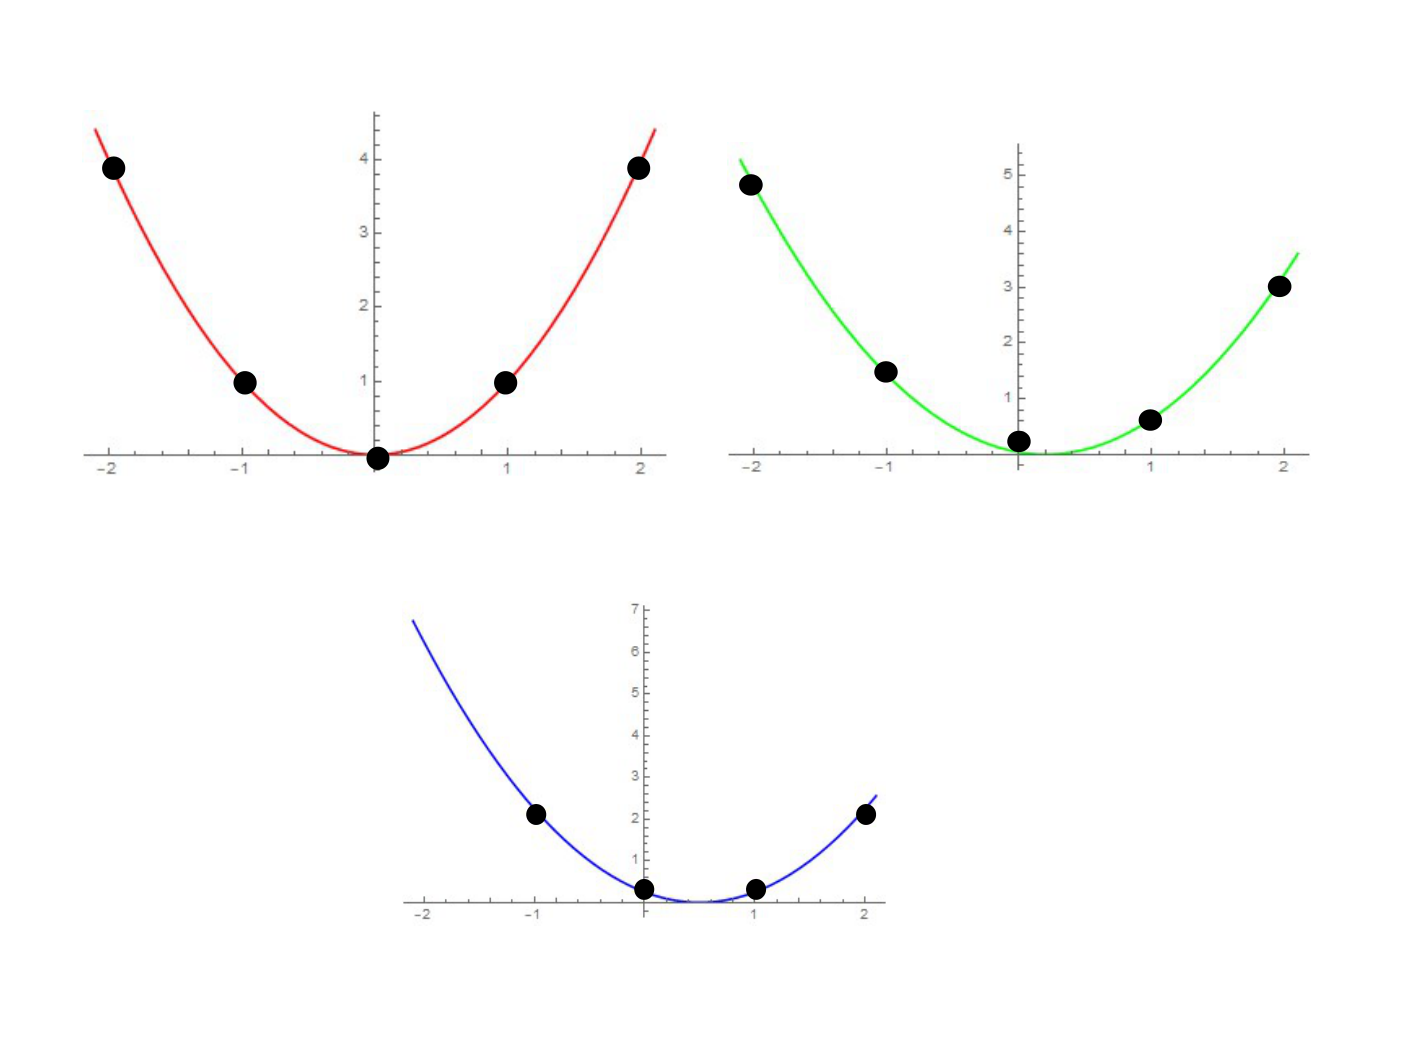
\includegraphics[width=0.85\textwidth]{figures/fig01.png}
  \caption{圆环上粒子的谱作为 $\mathcal{B}=eB/2\pi$ 的函数。左上图给出 $\mathcal{B}=0$ 时的低能谱，它在 $m\to-m$ 下对称。右上图给出 $\mathcal{B}=0.2$ 时的谱，谱中没有对称性。下图给出 $\mathcal{B}=1/2$ 时的谱，此时又有对称性，但对称操作是 $m\to2\mathcal{B}-m=1-m$。一般地，除非 $2\mathcal{B}\in\mathbb{Z}$，否则不会有任何对称性；若 $2\mathcal{B}\in\mathbb{Z}$，则谱在 $m\to2\mathcal{B}-m$ 下对称。（原文 Fig.~1，第 10 页）}
  \label{fig:1}
\end{figure}

第二项是「拓扑项」（topological term）或「$\theta$ 项」（$\theta$-term）的一个例子。经典地，第二项不影响物理预言，因为它是全导数。然而在量子力学层面，它会对物理预言产生重要影响。

我们将分析这个系统的对称性，并比较它们在经典理论与量子理论中的实现方式。

我们先分析经典对称性。由于 $\theta$ 项不影响经典动力学，经典系统具有 $O(2)$ 对称性。我们可以旋转：$R(\alpha):e^{\mathrm{i}\phi}\to e^{\mathrm{i}\alpha}e^{\mathrm{i}\phi}$；或者，如果你愿意，平移 $\phi\to\phi+\alpha$（始终记住 $\alpha$ 与 $\phi$ 只在模去 $2\pi$ 的整数倍的意义下有定义）。如果我们把圆环想成 $x-y$ 平面内以原点为心、螺线管沿 $z$ 轴的圆，那么我们也可以照例取

\begin{equation}
  R(\alpha)=
  \begin{pmatrix}
    \cos\alpha & \sin\alpha\\
    -\sin\alpha & \cos\alpha
  \end{pmatrix}
  \tag{2.4}
  \label{eq:2.4}
\end{equation}

此外我们还可以作「宇称」（parity）或「电荷共轭」（charge conjugation）变换 $P:\phi\to-\phi$。Lagrangian 中的第二项并不是不变的，但这「不要紧」，因为它是全导数。换个说法：$\phi\to-\phi$ 是运动方程的一个对称性。

注意 $O(2)$ 中这些群元素满足

\begin{gather}
  R(\alpha)R(\beta)=R(\alpha+\beta) \notag\\
  P^{2}=1 \notag\\
  PR(\alpha)P=R(-\alpha)
  \tag{2.5}
  \label{eq:2.5}
\end{gather}

而确实，正如我们已经看到的，$O(2)$ 是一个半直积（semidirect product）：

\begin{equation}
  O(2)=SO(2)\rtimes\mathbb{Z}_2
  \tag{2.6}
  \label{eq:2.6}
\end{equation}

其中同态 $\omega:\langle P\rangle\cong\mathbb{Z}_2\to Aut(SO(2))\cong\mathbb{Z}_2$ 把 $\mathbb{Z}_2$ 的非平凡元送到那个把 $R(\alpha)\mapsto R(-\alpha)$ 的外自同构。

\underline{把系统看作场论。}

我们引入这个系统时，把它描述为单个粒子的量子力学。然而重要的是注意到，它也可以被看作量子场论的一个特例。一般地，在场论中我们有一个时空 $M$，而场是 $M$ 上取值于某个目标空间（target space）$\mathcal{X}$ 的函数。（所以「目标空间」这个词的意思不多不少，就是场的余域。）在我们的情形里 $M=\mathbb{R}$，解释为时间实轴，而 $\mathcal{X}$ 是圆。于是我们的场是映射

\begin{equation}
  e^{\mathrm{i}\phi}:M\to S^{1}
  \tag{2.7}
  \label{eq:2.7}
\end{equation}

其中 $M$ 是时间实轴，或者也许是某个时间区间。后面我们还会取 $M$ 为圆。场空间是 $Map[M\to\mathcal{X}]$。由于 $M$ 是时间的一维流形，我们称此为「0+1 维场论」。我们一直把 $\phi\to-\phi$ 称作「宇称」，因为在平面内被约束在圆上的粒子之量子力学语境中，这是恰当的说法。然而，若采取「我们在讨论一个 0+1 维『场论』」的观点，那么最好把这个操作称为「电荷共轭」，因为它对 $U(1)$ 值的场 $e^{\mathrm{i}\phi}$ 取复共轭。

此外还有（在场论解释下）时间平移不变性与时间反演这两种「世界面（worldvolume）对称性」。它们构成群 $\mathbb{R}\rtimes\mathbb{Z}_2$。我们将把它们放到一边。（注意时间反演不是 Lagrangian 中第二项的对称性，但它是运动方程解空间的对称性。）

\underline{量子理论中的对称性。}

现在让我们考虑把「$\theta$ 项」加到 Lagrangian 之后的量子力学。我们的目标是看清该项如何影响量子理论。

我们先在哈密顿量（Hamiltonian）途径中分析量子力学。关于路径积分途径的一些评论见下面的注记。共轭动量（conjugate momentum）是

\begin{equation}
  L=I\dot\phi+\frac{eB}{2\pi}
  \tag{2.8}
  \label{eq:2.8}
\end{equation}

我们用 $L$ 记它，因为可以把它看成角动量。

注意，与平坦规范场的耦合改变了角动量与速度之间的通常关系。现在由 Legendre 变换得到哈密顿量：

\begin{equation}
  \int L\dot\phi\,dt-S=\int\frac{1}{2I}\Big(L-\frac{eB}{2\pi}\Big)^{2}dt
  \tag{2.9}
  \label{eq:2.9}
\end{equation}

量子化之后\footnote{这里可以再加一个常数。它会在量子化故事中引入第二个参数，但与 $\mathcal{B}$ 冗余。} $L\to-\mathrm{i}\hbar\frac{\partial}{\partial\phi}$，于是哈密顿量为

\begin{equation}
  H_{\mathcal{B}}:=\frac{\hbar^{2}}{2I}\Big(-\mathrm{i}\frac{\partial}{\partial\phi}-\mathcal{B}\Big)^{2}
  \tag{2.10}
  \label{eq:2.10}
\end{equation}

其中 $\mathcal{B}:=\frac{eB}{2\pi\hbar}$。

哈密顿量 $H_{\mathcal{B}}$ 的本征函数就是

\begin{equation}
  \Psi_m(\phi)=\frac{1}{\sqrt{2\pi}}e^{\mathrm{i}m\phi}
  \qquad m\in\mathbb{Z}
  \tag{2.11}
  \label{eq:2.11}
\end{equation}

它们给出能量本征态，其能量为

\begin{equation}
  E_m=\frac{\hbar^{2}}{2I}(m-\mathcal{B})^{2}
  \tag{2.12}
  \label{eq:2.12}
\end{equation}

对每个 $m\in\mathbb{Z}$ 恰有一个能量本征态。

% [Tutor Note: (2.9)$\to$(2.10) 这一步省略了代数：由 $L=I\dot\phi+\frac{eB}{2\pi}$ 得 $\dot\phi=(L-\frac{eB}{2\pi})/I$，代回 $H=L\dot\phi-\mathcal{L}$ 才得 $\frac{1}{2I}(L-\frac{eB}{2\pi})^2$；再令 $L\to-\mathrm{i}\hbar\partial_\phi$ 并把 $\frac{eB}{2\pi}$ 除以 $\hbar$ 写成 $\mathcal{B}$，才有 (2.10)。易错之处：$\mathcal{B}$ 里含 $\hbar$，而 $B$ 不含，混用会使 (2.12) 的周期判据从 $2\mathcal{B}\in\mathbb{Z}$ 错成 $2\pi\mathcal{B}\in\mathbb{Z}$；(2.11) 中 $m$ 取整数则来自 $\phi\sim\phi+2\pi$，即目标空间是圆——这正好回答了注 1 末尾的提问。]

\textbf{Remarks（注记）：}

\begin{enumerate}
  \item 作用量 (2.31) 无论对取值于实轴的 $\phi$，还是对取值于圆、满足 $\phi\sim\phi+2\pi$ 的 $\phi$，都完全说得通。作这个选择对于确定我们在描述哪个理论很重要。在上面的分析中——我们究竟在哪里作出了「目标空间是圆」这一选择？\footnote{\emph{答}：如果我们取 $\phi$ 取值于 $\mathbb{R}$ 而非圆的情形，那么对 $m$ 就没有量子化，哈密顿量的谱将是连续的。在这种情形下，Chern-Simons 项在量子力学版本中同样不会影响物理。}
  \item 取 $\phi\sim\phi+2\pi$ 之后，尽管 $\theta$ 项是全导数，它对量子物理仍有非平凡的影响——这一点我们可以从 $B$ 以物理上可观测的方式移动了量子哈密顿量的谱看出来：\emph{这就是我们看出拓扑项要紧的方式。}
  \item 注意当 $2\mathcal{B}$ 为偶数时，能量本征空间是二重简并的，只有位于 $m=\mathcal{B}$ 的基态例外。另一方面，当 $2\mathcal{B}$ 为奇数时，所有能量本征空间都是二重简并的，包括基态。若 $2\mathcal{B}$ 不是整数，则所有能量本征空间都是一维的。见图~\ref{fig:1}。
  \item 整个谱关于 $\mathcal{B}$ 是\emph{周期的}，且平移 $\mathcal{B}\to\mathcal{B}+1$ 等价于 $m\to m+1$。更精确地说，我们可以用在完备基上的作用来定义 Hilbert 空间上的一个酉算符：
\end{enumerate}

\begin{equation}
  U\Psi_m=\Psi_{m+1}
  \tag{2.13}
  \label{eq:2.13}
\end{equation}

以及

\begin{equation}
  UH_{\mathcal{B}}U^{-1}=H_{\mathcal{B}+1}
  \tag{2.14}
  \label{eq:2.14}
\end{equation}

\begin{enumerate}[start=5]
  \item 量子力学问题 (2.31) 与谱 \eqref{eq:2.12} 出现在量子点物理中「Coulomb 阻塞」（Coulomb blockade）的讨论里。参见 Yoshimasa Murayama，\emph{Mesoscopic Systems}，第 10.10 节。
  \item \emph{与高维场论及弦论的关系。} 我们加进来的 $\theta$ 项，在 $1+1$ 维场论中有一个非常有趣的对应物，在那里它被称为与 $B$-场的耦合。它也可以由 $1+1$ 维 Maxwell 理论的 Kaluza-Klein 约化得到：
\end{enumerate}

\begin{equation}
  S=\frac{1}{e^{2}}\int F\ast F+\int\frac{\theta}{2\pi}F
  \tag{2.15}
  \label{eq:2.15}
\end{equation}

在 $1+1$ 维理论中，我们可以取 $A_0=0$ 规范并规范掉对 $x^{1}$ 的依赖，于是在 $S^{1}\times\mathbb{R}$ 上唯一规范不变的量是

\begin{equation}
  e^{\mathrm{i}\phi(t)}=e^{\mathrm{i}\oint_{S^{1}}A}=e^{\mathrm{i}\oint_{S^{1}}A_1dx^{1}}
  \tag{2.16}
  \label{eq:2.16}
\end{equation}

有了这一点，我们可以说

\begin{equation}
  \theta=2\pi\mathcal{B}
  \tag{2.17}
  \label{eq:2.17}
\end{equation}

\textbf{Remark：}更一般地，在 $S^{1}\times\mathbb{R}$ 上的 $1+1$ 维 Yang-Mills 理论中，我们总可以走到 $A_0=0$ 规范，此时唯一规范不变的可观测量是绕圆的和乐（holonomy）的共轭类。

% [Tutor Note: 原文 p.12 注 1 与 p.13 注 5 两处把作用量编号写作 (2.31)，而本片段的作用量是 (2.1)（原书 (2.31) 是后文另一式）。据上下文判断这是作者的交叉引用笔误，译文照原样保留 (2.31) 不擅改，读者应回看 (2.1)。]

$\theta$ 项在 $3+1$ 维规范理论中也有一个密切的对应物。在 $3+1$ 维 Maxwell 理论的情形，我们可以写下

\begin{equation}
  S=\int d^{4}x\,\frac{1}{4e^{2}}F_{\mu\nu}F^{\mu\nu}+\int\frac{\theta}{(2\pi)^{2}}F\wedge F
  \tag{2.18}
  \label{eq:2.18}
\end{equation}

事实上，在存在绝缘体时电磁学的有效理论中，会出现一个非常相似、带 $\theta$ 项的作用量。如果存在宇称和/或时间反演对称性，那么 $\theta$ 为零或 $\pi$，对应于我们的情形 $2\mathcal{B}\in\mathbb{Z}$。于是普通绝缘体与拓扑绝缘体（topological insulator）之间的差别，字面上就是 $2\mathcal{B}$ 为偶数（普通）与为奇数（拓扑）的差别。最后，在描述弱、强相互作用标准模型的 $3+1$ 维 Yang-Mills 理论中，人们可以加入一个类似的 $\theta$ 项。关于自然的一个伟大未解之谜是：标准模型中强相互作用的（有效）theta 角为何小到无法测量。

现在，如果我们考察 $O(2)$ 对称性在量子理论中如何实现，我们会发现一个意外：

% 该编号列表在原 p.13 页末被切断：第 2 项起接续于下一片段（c02）。
\begin{enumerate}
  \item 经典理论具有 $O(2)$ 对称性。
\end{enumerate}

% =====================================================================
%  c02：原印刷页 14–21（PDF p.15–22）
%  内容：§2.1.1 页末编号列表的第 2–4 项（第 1 项由 c01 末尾引出）、§2.1.2、
%        §2.1.3、§2.2、§2.2.1、§2.2.2（至 p.21 页末的 Remarks 标题）。
%  本片段从编号列表中部起，故不补标题；全片段没有 \section 级标题，
%  因此不插入 keytakeaways。本片段无插图；编号公式 (2.19)–(2.49) 连续。
% =====================================================================

\begin{enumerate}[start=2]
  \item 在量子理论中，当 $2\mathcal{B}=\theta/\pi$ 不是整数时，对称性破缺为 $SO(2)$。

  \item 在量子理论中，当 $2\mathcal{B}=\theta/\pi$ 为偶数时，理论仍然具有 $O(2)$ 对称性。

  \item 在量子理论中，当 $2\mathcal{B}=\theta/\pi$ 为奇数时，经典的 $O(2)$ 关系不再成立，但覆叠群 $\mathrm{Pin}^{+}(2)$ 是一个对称性。
\end{enumerate}

我们要强调，圆环上的粒子\underline{并不是}自旋二分之一！！话虽如此，如果我们定义角动量 $\mathcal{L}$，使得 $H=\frac{\mathcal{L}^{2}}{2I}$，那么当 $\mathcal{B}$ 为半整数时，角动量确实具有半整数本征值，一如人们对自旋表示所期待的那样。所以我们得到的是：半通量量子（half flux quantum）在诱导这个系统的半整数自旋，从而经典系统的经典 $O(2)$ 对称性在量子理论中被实现为 $\mathrm{Pin}^{+}(2)$ 对称性。这是出现在带非平凡规范场与 Chern-Simons 项的量子对称性中的一个耐人寻味的现象：粒子的统计与自旋可以相对其经典值发生移动，而且往往是以牵涉古怪分数的形式移动。

\subsubsection{围绕螺线管的圆环上的带电粒子：路径积分} % 原文: 2.1.2 Charged Particle On A Circle Surrounding A Solenoid: Path Integrals

用两种办法计算这个理论的欧氏时间传播子会很有启发性。于是我们考虑量 $\langle\phi_2|e^{-\beta H}|\phi_1\rangle$。一方面，我们已经把哈密顿量完全对角化，所以插入一组完备态便立刻得到：

\begin{equation}
  \langle\phi_2|e^{-\beta H_{\mathcal{B}}}|\phi_1\rangle=\frac{1}{2\pi}\sum_{m\in\mathbb{Z}}e^{-\frac{\beta}{2I}(m-\mathcal{B})^{2}+\mathrm{i}m(\phi_1-\phi_2)}
  \tag{2.19}
  \label{eq:2.19}
\end{equation}

% [Tutor Note: (2.19) 最容易出错的是相位里 $(\phi_1-\phi_2)$ 的次序与符号。用 $\Psi_m(\phi)=\frac{1}{\sqrt{2\pi}}e^{\mathrm{i}m\phi}$（见 \eqref{eq:2.11}）作完备性插入：$\langle\phi_2|e^{-\beta H_{\mathcal{B}}}|\phi_1\rangle=\sum_m\langle\phi_2|m\rangle e^{-\beta E_m}\langle m|\phi_1\rangle=\frac{1}{2\pi}\sum_m e^{\mathrm{i}m\phi_2}e^{-\beta E_m}e^{-\mathrm{i}m\phi_1}$，正是 $e^{\mathrm{i}m(\phi_1-\phi_2)}$。若把 $\langle\phi_2|\cdots|\phi_1\rangle$ 的左右次序写反，就会得到 $e^{\mathrm{i}m(\phi_2-\phi_1)}$，而 (2.19) 与 (2.23) 之间的一次 theta 变换核对将失败；这个符号也正是下一段 (2.20) 里作者提醒「必须小心虚项的符号，而且它很要紧」的那个符号。]

另一方面，利用传播子的 Feynman 路径积分表示作 Wick 转动，我们也可以得到一个用路径积分表达的式子：

\begin{equation}
  \langle\phi_2|e^{-\beta H}|\phi_1\rangle=Z(\phi_2,\phi_1|\beta):=\int[d\phi(t)]_{\phi(0)=\phi_1}^{\phi(\beta)=\phi_2}e^{-\frac{1}{\hbar}\int_0^{\beta}\frac{1}{2}I\dot\phi^{2}dt-\mathrm{i}\int\mathcal{B}\dot\phi dt}
  \tag{2.20}
  \label{eq:2.20}
\end{equation}

注意，在转到欧氏号差的这一步中，拓扑项仍然是虚的。必须小心取准这个虚项的符号，而它很要紧。

把这个理论看作场论，那么它是一个自由场论，其路径积分可以用半经典技巧精确计算：

运动方程简单地就是 $\ddot\phi=0$。同样，$\theta$ 项并没有改变它。

于是，带有边界条件 $\phi(0)=\phi_1$、$\phi(\beta)=\phi_2$ 的运动方程的经典解为：

\begin{equation}
  \phi_{cl}(t)=\phi_1+\left(\frac{\phi_2-\phi_1+2\pi w}{\beta}\right)t
  \qquad w\in\mathbb{Z}
  \tag{2.21}
  \label{eq:2.21}
\end{equation}

或者更切题地说：

\begin{equation}
  e^{\mathrm{i}\phi_{cl}(t)}=e^{\mathrm{i}\left(\left(1-\frac{t}{\beta}\right)\phi_1+\frac{t}{\beta}\phi_2\right)+\frac{2\pi\mathrm{i}tw}{\beta}}
  \tag{2.22}
  \label{eq:2.22}
\end{equation}

这些是欧氏运动方程的解，由于历史的原因被称为「瞬子」（instantons）。注意，由于我们定义这个 $0+1$ 维场论时所处的时空是紧致的，这样的解有无穷多个，以 $w\in\mathbb{Z}$ 标记。这个游戏里有两个圆：这个 $0+1$ 维场论的时空是欧氏时间圆；而场论的目标空间也是一个圆。量子的场 $e^{\mathrm{i}\phi(t)}$ 是一个映射 $M\to\mathcal{X}$。$M$ 是时空，它是 $S^{1}$；而 $\mathcal{X}$ 是目标空间，它也是 $\mathcal{X}$。回忆 $\pi_1(S^{1})\cong\mathbb{Z}$。可以存在拓扑上不等价的场构型。也就是说，映射空间 $Map(M\to\mathcal{X})$ 有不同的连通分支。不同的拓扑扇区由映射 \eqref{eq:2.22} 的绕数（winding number）唯一地标记。在路径积分里我们对所有场构型求和，因此也应当对所有这些瞬子构型求和。

% [Tutor Note: 原文此句「$\mathcal{X}$，也就是目标空间，也是 $\mathcal{X}$」显然是笔误，依据上一句应读作「也是 $S^{1}$」；照原文转写，未改。另需注意 $e^{\mathrm{i}\phi}$ 是映射 $M\to\mathcal{X}$，而不是 $\phi$ 本身——$\phi$ 只是 $\mathbb{R}$ 值的一个「抬升」，它在绕 $M$ 走一圈时只能回到模 $2\pi$ 的同一个值，绕数 $w$ 正是这个抬升的单值性障碍，也就是 $M$ 的 $\pi_1$ 到 $\mathcal{X}=S^{1}$ 的 $\pi_1$ 的映射度。]

一个直接的计算（细节见在线讲义 [48]）表明，路径积分表达式恰好等于

\begin{equation}
  Z(\phi_2,\phi_1|\beta)=\sqrt{\frac{I}{2\pi\beta}}\sum_{w\in\mathbb{Z}}e^{-\frac{2\pi^{2}I}{\beta}\left(w+\frac{\phi_2-\phi_1}{2\pi}\right)^{2}-2\pi\mathrm{i}\mathcal{B}\left(w+\frac{\phi_2-\phi_1}{2\pi}\right)}
  \tag{2.23}
  \label{eq:2.23}
\end{equation}

% [Tutor Note: 此处作者以「a straightforward computation（一个直接的计算）」跳过全部推导，只指向在线讲义 [48]。被略去的是两件事：一是围绕 (2.21)–(2.22) 的经典解作二次涨落积分，涨落算符为 $-\frac{I}{\hbar}\partial_t^{2}$（配以 Dirichlet 边界条件），其行列式给出前置因子 $\sqrt{I/2\pi\beta}$——(2.19) 中已取 $\hbar=1$，与 (2.20) 里显式的 $1/\hbar$ 对照即可定出这一因子；二是把「按 $w$ 求和」与「按 $m$ 求和」联系起来的 Poisson 求和公式，这才是 (2.23) 与 (2.19) 相等这一「看似神奇」的数学事实的真正内容，也正是紧接着 (2.24)–(2.25) 要给出的 theta 函数机制。核对符号时请记住：拓扑项给出的相位是 $-2\pi\mathrm{i}\mathcal{B}w$，其符号与 (2.20) 中的 $-\mathrm{i}\int\mathcal{B}\dot\phi dt$ 一致。]

现在比较 \eqref{eq:2.19} 与 \eqref{eq:2.23}。这两个表达式看上去大不相同！一个涉及以 $\beta$ 在分子上的指数之和，另一个则是 $\beta$ 在分母上。前者适合讨论 $\beta\to\infty$（低温）的渐近行为，后者适合讨论 $\beta\to0$（高温）。然而，我们算出的是同一个物理量，只是用了两种不同的方法，所以它们必定相等。但那个说它们相等的数学恒等式看起来颇有几分神奇。下面我们说明如何用一个直接的数学论证来验证这两个表达式确实完全相同。

我们引入 Riemann theta 函数

\begin{equation}
  \vartheta\left[\genfrac{}{}{0pt}{}{\theta}{\phi}\right](z|\tau):=\sum_{n\in\mathbb{Z}}e^{\mathrm{i}\pi\tau(n+\theta)^{2}+2\pi\mathrm{i}(n+\theta)(z+\phi)}
  \tag{2.24}
  \label{eq:2.24}
\end{equation}

Riemann theta 函数是 $\tau$ 在上半平面内的绝对收敛解析函数，它也是 $z$ 的整函数。利用 Poisson 求和公式可以验证关键的模变换律：

\begin{equation}
  \vartheta\left[\genfrac{}{}{0pt}{}{\theta}{\phi}\right]\left(\frac{-z}{\tau}\Big|\frac{-1}{\tau}\right)=(-\mathrm{i}\tau)^{1/2}e^{2\pi\mathrm{i}\theta\phi}e^{\mathrm{i}\pi z^{2}/\tau}\,\vartheta\left[\genfrac{}{}{0pt}{}{-\phi}{\theta}\right](z|\tau)
  \tag{2.25}
  \label{eq:2.25}
\end{equation}

% [Tutor Note: 「用 Poisson 求和公式可以验证」跳过的正是全部计算：把 $\sum_n\delta(x-n)$ 展成 $\sum_k e^{2\pi\mathrm{i}kx}$ 后再逐项作高斯积分，才会同时得到前置因子 $(-\mathrm{i}\tau)^{1/2}$、指数上的 $e^{\mathrm{i}\pi z^{2}/\tau}$，以及特征（characteristic）的交换 $\left[\genfrac{}{}{0pt}{}{\theta}{\phi}\right]\to\left[\genfrac{}{}{0pt}{}{-\phi}{\theta}\right]$（注意这不是简单的 $\theta\leftrightarrow\phi$，两处各带一个负号）。$(-\mathrm{i}\tau)^{1/2}$ 的平方根分支不可随意取：$\tau$ 在上半平面时须取主分支，否则 (2.25) 会整体多一个负号。用 (2.25) 核对传播子时，要点在于 $\tau$ 在此取纯虚值（$\tau\propto\mathrm{i}\beta$），于是模变换 $\tau\to-1/\tau$ 恰好把 $\beta\to0$ 与 $\beta\to\infty$ 互换——这正是 (2.19) 适合低温、而 (2.23) 适合高温的根源；同时还要把 $\mathcal{B}$ 与 $\frac{\phi_2-\phi_1}{2\pi}$ 分别对号入座地塞进特征 $(\theta,\phi)$，否则 (2.19) 的 $m$ 求和与 (2.23) 的 $w$ 求和很容易被互换，而丢掉 $2\pi\mathrm{i}\mathcal{B}(\cdots)$ 这一相位。]

可以很容易地核验：上面给出的欧氏传播子的两个公式，正是由 Riemann theta 函数的模变换联系起来的。

我们将会看到，theta 函数及其模性质在后文将起重要作用。

\medskip\noindent\textbf{练习}\quad 设 $2\mathcal{B}$ 为奇数。

\begin{enumerate}[label=\alph*.)]
  \item 证明：当 $\beta\to\infty$ 时，

\begin{equation}
  \langle\phi_2|e^{-\frac{\beta H}{\hbar}}|\phi_1\rangle\sim 2e^{\frac{\mathrm{i}}{2}(\phi_1-\phi_2)}\cos\left(\frac{\phi_1-\phi_2}{2}\right)e^{-\beta E_{\mathrm{ground}}}+\cdots
  \tag{2.26}
  \label{eq:2.26}
\end{equation}

  \item 注意这个表达式在 $\phi\to-\phi$ 下并不保持不变。但在 $\mathrm{Pin}^{+}(2)$ 中存在一个元素 $P$，它对应 $\phi\to-\phi$。这与我们关于 $\mathrm{Pin}^{+}(2)$ 是量子理论的一个合法对称性的论证如何相容？\footnote{\emph{答}：见 [48]。}
\end{enumerate}

\subsubsection{对整体 $SO(2)$ 对称性作规范化与 Chern-Simons 项} % 原文: 2.1.3 Gauging The Global $SO(2)$ Symmetry And Chern-Simons Terms

% [Tutor Note: 术语取舍。「gauging a symmetry」在中文文献里有「规范化」「局域化」「引规范」「把对称性变成规范对称性」等说法，本译本统一作「规范化」，并在首次出现处括注英文；但须与「normalization（归一化）」区分——同一页上（原 p.19 起）作者反复讲 normalizations 指的是耦合常数与曲率的归一化，两者不可混同。另外，这里的「gauging」是两步：先局域化并耦合规范场，再对规范场积分；只做第一步时称「与（非动力学）外源规范场耦合」，不要把它等同于「把规范场量子化」。]

当一个理论具有对称性时，人们可以实施一个称为「规范化」（gauging the symmetry）的程序。这是一个两步过程：

\begin{enumerate}
  \item 把对称性变成局域的，并耦合到一个规范场；
  \item 对规范场积分。
\end{enumerate}

并不需要在完成第 (1) 步之后接着做第 (2) 步。在这种情形下，我们说是在与\emph{非动力学的外源规范场}（nondynamical external gauge fields）耦合。为一个对称性引入非动力学的外源规范场是完全可以的。我们在量子力学课上一直这么干：把量子系统耦合到电磁场，却并不试图去量子化那个电磁场。

对数学修养更好的读者，这个两步过程可以概括为：给定一个具有对称群 $G$ 的场论，我们可以通过改变其定义域所在的配边范畴（bordism category）来使该理论成为 $G$-等变的：

\begin{enumerate}
  \item 把对称群等同于某个主丛的结构群，并把场论的几何定义域改为带联络的丛；
  \item 对主丛的同构类求和，并对联络积分。
\end{enumerate}

我们将在第 {\small\itshape ［原文标记：****］}% [原文待办标记：交叉引用的节号未填，原文 p.16 印作「in section ****」]
节中对此再多作一点解释。

在目前这个简单的例子里，我们可以把对所有 $\mathcal{B}$ 值都存在的整体 $SO(2)$ 对称性 $\phi\to\phi+\alpha$ 加以「规范化」。\footnote{于是，看看外源规范场如何告诉我们关于电荷共轭对称性的信息，就很有意思了。关于这一点的一个讨论见 D. Gaiotto、A. Kapustin、Z. Komargodski 与 N. Seiberg，\emph{Theta, Time Reversal, and Temperature}，\url{https://arxiv.org/pdf/1703.00501.pdf} 的附录 D。}

于是，在我们这个简单例子里，我们把这个平移对称性变成局域的，也就是说，我们试图把

\begin{equation}
  \phi(t)\to\phi(t)+\alpha(t)
  \tag{2.27}
  \label{eq:2.27}
\end{equation}

变成一个对称性，其中 $\alpha(t)$ 不是常数，而是时间的「任意」函数。当然，作用量 $\sim\int\dot\phi^{2}$ 在这样的变换下并不不变。我们引入一个规范场 $A_t^{(e)}dt$，其中上标 $e$ 表示「外源的」（external），提醒我们这\underline{不是}电磁场的规范场。（那个场已经产出了我们的 theta 项。）相反，它是我们系统中的一个新场：转动对称性的规范场。

规范化后的作用量是

\begin{equation}
  S=\int\frac{1}{2}I(\dot\phi+A_t^{(e)})^{2}dt+\oint\mathcal{B}(\dot\phi+A_t^{(e)})dt
  \tag{2.28}
  \label{eq:2.28}
\end{equation}

它在如下规范变换下是规范不变的：

\begin{gather}
  \phi\to\phi+\alpha(t)\notag\\
  A_t^{(e)}\to A_t^{(e)}-\partial_t\alpha(t)
  \tag{2.29}
  \label{eq:2.29}
\end{gather}

或者，更好的写法是

\begin{gather}
  e^{\mathrm{i}\phi(t)}\to e^{\mathrm{i}\phi(t)}e^{\mathrm{i}\alpha(t)}\notag\\
  A_t^{(e)}\to A_t^{(e)}+\mathrm{i}e^{-\mathrm{i}\alpha(t)}\partial_te^{\mathrm{i}\alpha(t)}
  \tag{2.30}
  \label{eq:2.30}
\end{gather}

这样更好，是因为在拓扑非平凡的时空上工作时——例如在欧氏时间圆上——应当满足单值性的是 $e^{\mathrm{i}\alpha(t)}$。

在没有外源规范场 $A_t^{(e)}$ 时，我们发现 $\mathcal{B}$ 是模一个整数周期的。往作用量里加一个 Chern-Simons 项，我们就能把某种周期性还给 $\mathcal{B}$。在欧氏空间中，新的作用量是：

\begin{equation}
  e^{-S}=e^{-\int\frac{1}{2}I(\dot\phi+A_t^{(e)})^{2}dt-\mathrm{i}\oint\mathcal{B}(\dot\phi+A_t^{(e)})dt}\,e^{\mathrm{i}k\int A_t^{(e)}dt}
  \tag{2.31}
  \label{eq:2.31}
\end{equation}

我们手工地把不变性恢复了出来，使得带有 $(\mathcal{B},k)$ 的新理论等价于带有 $(\mathcal{B}+1,k+1)$ 的理论。但现在我们必须操心新加这一项的规范不变性。这里有一个关键点：

\begin{center}
  \fbox{\parbox{0.92\textwidth}{\itshape 作用量本身不必保持不变。要有一个良定义的路径积分，所需的全部只是：指数化后的作用量必须不变。}}
\end{center}

我们后面还会多次援引这一观察：在量子化作用量中其它 Chern-Simons 项的系数时，以及在讨论二维 CFT 中的 WZ 项时。我们将称之为\emph{多值作用量原理}（multi-valued action principle）：作用量 $S$ 可以是多值的，只要 $e^{\mathrm{i}S}$ 是单值的。

因此，我们来研究

\begin{equation}
  e^{\mathrm{i}k\oint A_t^{(e)}dt}
  \tag{2.32}
  \label{eq:2.32}
\end{equation}

的规范不变性。

现在我们必须决定自己在哪个 1-流形上工作。

在区间 $[t_1,t_2]$ 上，表达式

\begin{equation}
  \exp\left[\mathrm{i}\int_{t_1}^{t_2}A_t^{(e)}(t')dt'\right]
  \tag{2.33}
  \label{eq:2.33}
\end{equation}

不是规范不变的。更确切地说：

\begin{equation}
  \exp\left[\mathrm{i}\int_{t_1}^{t_2}A_t^{(e)}(t')dt'\right]\to e^{-\mathrm{i}\alpha(t_2)}\exp\left[\mathrm{i}\int_{t_1}^{t_2}A_t^{(e)}(t')dt'\right]e^{\mathrm{i}\alpha(t_1)}
  \tag{2.34}
  \label{eq:2.34}
\end{equation}

因此，在实直线上，只要选取边界条件使得 $\alpha(t)$ 当 $t\to\pm\infty$ 时趋于零，$\exp\left[\mathrm{i}\int_{\mathbb{R}}A_t^{(e)}(t')dt'\right]$ 就是规范不变的。

类似地，在圆上，如果 $\alpha(t)$ 是单值的，那么

\begin{equation}
  \exp\left[\mathrm{i}\oint_{S^{1}}A_t^{(e)}(t')dt'\right]
  \tag{2.35}
  \label{eq:2.35}
\end{equation}

是规范不变的。然而对圆来说，真正的规范参数是 $g(t)=e^{\mathrm{i}\alpha(t)}$（对 $U(1)$ 规范群而言）。因此，$\alpha(t)=2\pi wt/\beta$（$w\in\mathbb{Z}$）是一个合法的规范变换；但在这样的规范变换下：

\begin{equation}
  \exp\left[\mathrm{i}k\oint_{S^{1}}A_t^{(e)}(t')dt'\right]\to e^{2\pi\mathrm{i}wk}\exp\left[\mathrm{i}k\oint_{S^{1}}A_t^{(e)}(t')dt'\right]
  \tag{2.36}
  \label{eq:2.36}
\end{equation}

因此，如果我们想要让理论在圆上说得通，那么 $k$ 就应当被量子化为整数。一般地：$t\mapsto e^{\mathrm{i}\alpha(t)}$ 定义了一个映射 $S^{1}_{\mathrm{time}}\to U(1)$。但 $\pi_1(U(1),*)\cong\mathbb{Z}$ 由绕数刻画。当这个绕数非零时，我们说 $e^{\mathrm{i}\alpha(t)}$ 定义了一个\emph{大的规范变换}（large gauge transformation）。

{\itshape「Chern-Simons 项」在大的规范变换下的规范不变性蕴含耦合常数是量子化的：$k\in\mathbb{Z}$。\par}

出于与电荷共轭对称性的实现有关的理由，把定义延拓到半整数的 $k$ 是有好处的。有办法赋予半整数量子化的 Chern-Simons 项以意义，那就是把 $0+1$ 维理论看作某个良定义的 $1+1$ 维理论的边界。由 Stokes 定理我们有：

\begin{equation}
  \exp\left[\mathrm{i}k\oint_{S^{1}}A_t^{(e)}dt\right]=\exp\left[\mathrm{i}k\int_{\Sigma}F^{(e)}\right]
  \tag{2.37}
  \label{eq:2.37}
\end{equation}

其中 $F^{(e)}=dA^{(e)}$。右端即使在 $k$ 不是整数时也说得通，但现在这个表达式依赖于 $1+1$ 维时空 $\Sigma$ 的「体内」（bulk）规范场的细节。

在真实的凝聚态系统中可以观测到一个非常类似的现象：$3+1$ 维拓扑绝缘体的边界理论，由能级为半整数的 Chern-Simons 理论描述。（也就是说，是朴素规范不变性所允许的能级的一半。）

\medskip\noindent\textbf{练习}\quad\emph{谜题}

解决如下悖论：

我们首先论证了：若 $k\notin\mathbb{Z}$，则 \eqref{eq:2.37} 的左端在大的规范变换下\underline{不是}不变的。然后我们又用右端的表达式来\emph{定义}左端，而右端是明显规范不变的。这两个论断如何相容？\footnote{\emph{答}：规范变换 $e^{\mathrm{i}\alpha(t)}$ 必须延拓为连续映射 $\Sigma\to U(1)$。若 $\Sigma$ 是一个光滑流形，其边界只有 $S^{1}$——这正是我们写下方程 \eqref{eq:2.37} 时默认的假设——那么这样的映射限制到作为其边界的 $S^{1}$ 上时，总是小规范变换。}

% [Tutor Note: 这条悖论的解答完全在于「延拓」二字（见上一条脚注），而不是在于 (2.37) 的等式本身：左端之所以能为半整数 $k$ 定义，靠的是把 $1+1$ 维的 $\Sigma$ 一并纳入定义，此时规范变换的参数 $\alpha$ 必须是 $\Sigma$ 上的整体定义的单值函数，它在边界 $S^{1}$ 上的绕数必为零，于是 (2.36) 里的 $e^{2\pi\mathrm{i}wk}$ 根本不会被激发。代价是：真正的半整数 Chern-Simons 项还需要额外的数据（旋量结构），本讲义后文（第 2.5 节；另见下一片段的 \eqref{eq:2.50} 前后）才展开这一点，此处不宜把半整数 $k$ 当成「无需额外数据」的结果使用。]

\subsection{三维中的 $U(1)$ Chern-Simons 理论} % 原文: 2.2 $U(1)$ Chern-Simons Theory In 3 Dimensions

\subsubsection{$U(1)$ 规范理论的若干预备知识} % 原文: 2.2.1 Some $U(1)$ Gauge Theory Preliminaries

在整份讲义中，我们将需要非常小心地对待归一化与周期性，所以我们把 $U(1)$ 规范理论的归一化明确写出来。

我们从某个时空 $M$ 上基于阿贝尔 Lie 群 $U(1)$ 或 $\mathbb{R}$ 的规范理论出发。局部地，规范场是一个实 1-形式，记作 $A=A_\mu dx^\mu$。我们要强调：虽然 $F=dA$ 是一个整体良定义的 2-形式，但一般来说 $A$ 并不是整体良定义的 1-形式，所以 $F$ 完全可能是一个非恰当（non-exact）的闭 2-形式。

更正式地说，$A$ 是 $M$ 上某个主 $U(1)$ 丛或复线丛上联络的局部 1-形式表示。在我们的归一化下，协变导数局部地写作 $D=d+\mathrm{i}A$，并在两片覆盖的交叠 $\mathcal{U}_\alpha\cap\mathcal{U}_\beta$ 上按 $D_\alpha=g_{\alpha\beta}^{-1}D_\beta g_{\alpha\beta}$ 变化。

\textbf{Remark：}\underline{一个重要的约定。}尽管从数学家的观点看这并非最好的归一化，我们这里仍取（局部定义的 1-形式）$A$ 在规范群为 $G=U(1)$ 时是一个\underline{实} 1-形式。当 $G=U(1)^{d}$ 时，我们继续取它是 $d$ 个局部定义 1-形式组成的 $d$-重 $A^{I}$。然而，在处理一般的非阿贝尔 Lie 群时，我们取 $A$ 是一个取值于 Lie 代数 $\mathfrak{g}$ 的 1-形式。现在，由于我们处理的是紧 Lie 群，若 $G$ 是一个矩阵群，则 $\mathfrak{g}$ 将是某个\underline{反厄米}矩阵 Lie 代数的子代数。在这一约定下，协变导数为 $D_A=d+A$。

如上所述，由于 $A$ 只是局部定义的，2-形式 $F$ 虽然整体有定义，却未必恰当。我们的规范场这样归一化，使得 $F/2\pi$ 具有整数周期，也就是说，绕闭 2-圈的积分总是整数：

\begin{equation}
  \int_{\Sigma_2}F\in 2\pi\mathbb{Z}
  \tag{2.38}
  \label{eq:2.38}
\end{equation}

对任何闭的定向 2-圈 $\Sigma_2\subset M$ 成立。此外，若规范群是 $G=U(1)$，则总存在流形 $M$、线丛 $L\to M$ 以及 2-圈 $\Sigma_2\subset M$，使得整数 $\int_{\Sigma_2}\frac{F}{2\pi}$ 恰好等于一。因此这是最优的归一化。反之，若规范群是 $G=\mathbb{R}$，则 $F$ 的周期将总是零。也就是说，$F$ 总是恰当的，而 $A$ 可以取为整体良定义的 1-形式。

在上述约定下，规范变换是这样的：协变导数 $D=d+\mathrm{i}A$ 按 $D\to g^{-1}Dg$ 变换，其中

\begin{equation}
  g:M\to U(1)
  \tag{2.39}
  \label{eq:2.39}
\end{equation}

是一个规范变换。如果我们能取对数，并对一个整体良定义的函数取 $g=e^{\mathrm{i}\epsilon}$，

\begin{equation}
  \epsilon:M\to\mathbb{R}
  \tag{2.40}
  \label{eq:2.40}
\end{equation}

那么

\begin{equation}
  A\to A-d\epsilon
  \tag{2.41}
  \label{eq:2.41}
\end{equation}

我们把这样的变换称为「小的规范变换」（small gauge transformations）。若规范群是 $\mathbb{R}$，则所有规范变换都是这个形式。另一方面，若规范群是 $U(1)$，则会出现不允许整体对数的映射 $g:M\to U(1)$。一个简单的判据是：1-形式 $\omega=-\mathrm{i}g^{-1}dg$ 是否有非零的周期。如果 $g(x)$ 不能写成 $g(x)=e^{\mathrm{i}\epsilon(x)}$（其中 $\epsilon(x)$ 是整体良定义的函数），我们就说 $g(x)$ 是一个「大的规范变换」。特别地，若 $\pi_1(M,x_0)$ 非平凡，则存在大的规范变换。在这种情形下，规范变换最好被设想为平移

\begin{equation}
  A\to A+\omega
  \qquad \omega\in\Omega^{1}_{2\pi\mathbb{Z}}(M)
  \tag{2.42}
  \label{eq:2.42}
\end{equation}

其中 $\Omega^{1}_{2\pi\mathbb{Z}}(M)$ 是所有（适当可微的）周期都落在 $2\pi\mathbb{Z}$ 中的闭 1-形式构成的空间。

% [Tutor Note: (2.41) 的符号必须与约定绑在一起核对。按正文自己给的 $D=d+\mathrm{i}A$、$D\to g^{-1}Dg$、$g=e^{\mathrm{i}\epsilon}$ 直接算：$g^{-1}(\partial+\mathrm{i}A)g=\partial+g^{-1}\partial g+\mathrm{i}A$，而 $g^{-1}\partial g=\mathrm{i}\partial\epsilon$，于是得到 $A\to A+d\epsilon$，与印出的 (2.41)「$A\to A-d\epsilon$」差一个符号。把相邻几式放在一起看会更清楚：(2.30) 的 $A_t^{(e)}\to A_t^{(e)}+\mathrm{i}e^{-\mathrm{i}\alpha}\partial_te^{\mathrm{i}\alpha}$ 其实等于 $A_t^{(e)}-\partial_t\alpha$，即 $\delta A=-d\alpha$；而 (2.45) 的右端 $d(\epsilon F)$ 在 $dF=0$ 时等于 $d\epsilon\wedge F$，对应的却是 $\delta A=+d\epsilon$（若与 (2.41) 配套，本应印成 $A\wedge F-d(\epsilon F)$）。也就是说，(2.30) 与 (2.41) 自相一致，而 (2.45) 取的是相反的一支；这源于原稿在「$A$ 取实值」与「$A$ 取反厄米」两种归一化之间往返。复算 $\kappa$ 的量子化条件、或把 (2.48) 的整体符号与别的文献对照时，务必先固定一支（例如 $\delta A=-d\epsilon$、$\omega=-\mathrm{i}g^{-1}dg$），不要跨式混用。]

此外，当 $M$ 非紧或者有非空边界时，我们还需要讨论规范场与规范群的边界条件。我们会考虑不同种类的边界条件，所以这一点留到后面再说。

\subsubsection{从 $\theta$ 项到 Chern-Simons} % 原文: 2.2.2 From $\theta$-term To Chern-Simons

现在，由于 $F=dA$，我们注意到四维的拓扑密度可以写成：

\begin{equation}
  F\wedge F=d(AdA)
  \tag{2.43}
  \label{eq:2.43}
\end{equation}

如果我们考虑一个 $\partial M_4=M_3$ 的四维路径积分（$M_3$ 可以连通，也可以不连通），那么我们就会被要求把

\begin{equation}
  \int_{M_3}AdA
  \tag{2.44}
  \label{eq:2.44}
\end{equation}

作为作用量中的一项来考虑。

初看起来，\eqref{eq:2.44} 不像是一个能放进规范理论作用量里的项：这一项明显含有 $A$ 这个因子，因此显然不是规范不变的。另一方面，$F\wedge F$ 是规范不变的，所以 $AdA$ 的变化必须是 $d$-闭的。我们可以指望它是 $d$-恰当的，从而「由全导数造成的变化无关紧要」。

那么，我们来算一算：

\begin{enumerate}
  \item 在小规范变换 \eqref{eq:2.41} 下，我们有

\begin{equation}
  A\wedge F\to A\wedge F+d(\epsilon F)
  \tag{2.45}
  \label{eq:2.45}
\end{equation}

  这确实是一个全导数，正如我们所希望的那样。如果忽略边界贡献（一般来说我们\underline{不能}这么做），那么规范不变性就有保证了。无论如何，这是一个好的开始。

  \item 在大规范变换 \eqref{eq:2.42} 下，我们有

\begin{equation}
  A\wedge F\to A\wedge F+\omega\wedge F
  \tag{2.46}
  \label{eq:2.46}
\end{equation}

  现在，任何具有量子化周期的 1-形式必定是闭 1-形式，但一般来说它不必整体恰当，所以 $\omega\wedge F$ 不必整体恰当。连同边界项的问题，这一点是我们需要处理的。
\end{enumerate}

\medskip\noindent\underline{$\kappa$ 的量子化}% 原文: Quantization Of $\kappa$（原以斜体下划线标示的无编号小标题，独占一行）
\par\vspace{2pt}

我们考虑在某个定向 3-流形 $M_3$ 上的 $U(1)$ 规范理论作用量中加入可能的 Chern-Simons 项，并把耦合常数归一化为：

\begin{equation}
  \exp\left[\mathrm{i}\frac{\kappa}{2\pi}\int_{M_3}A\wedge F\right]
  \tag{2.47}
  \label{eq:2.47}
\end{equation}

暂时我们取 $M_3$ 没有边界。即便在这种情况下，正如我们刚刚讨论过的，作用量并不是规范不变的。在路径积分中，我们并不对 $\mathcal{A}$——所有规范场（即固定主丛上的所有联络）构成的空间——积分，而是对 $\mathcal{A}/\mathcal{C}G$——所有规范等价类的空间——积分。这里 $\mathcal{G}$ 是规范变换构成的群。通过 Fadeev-Popov 或 BRST 型的程序，我们可以把 $\mathcal{A}$ 上的自然测度 $[dA]$ 推下来，成为 $\mathcal{A}/\mathcal{G}$ 上的一个测度；但这样一来，当我们用 $e^{\mathrm{i}S}$ 去权重这个测度时，那个因子必须是空间 $\mathcal{A}/\mathcal{G}$ 上的良定义且单值的函数。

当你看到作用量里出现一个显式的规范场时，你脑子里的所有警报都应当响起来：这个理论多半说不通。Chern-Simons 之所以能躲过这个问题，靠的就是上面提到的多值作用量原理。这个原理之所以适用，是因为该理论的路径积分是对 $\mathcal{A}/\mathcal{G}$（规范场的规范等价类空间）的积分，而我们所需要的一切，只是这个空间上的一个（形式上）良定义的测度 $[dA]e^{\mathrm{i}S}$。

让我们回到 \eqref{eq:2.46}。那么，正如我们刚刚指出的，Chern-Simons 作用量 $\int_{M_3}AdA$ \underline{不是}规范不变的。在 \eqref{eq:2.46} 下，指数化作用量的变化是一个乘性因子：

\begin{equation}
  e^{2\pi\mathrm{i}\frac{\kappa}{4\pi^{2}}\int_{M_3}A\wedge dA}\to e^{2\pi\mathrm{i}\frac{\kappa}{4\pi^{2}}\int_{M_3}A\wedge dA}\cdot e^{2\pi\mathrm{i}\kappa\int_{M_3}\frac{\omega}{2\pi}\wedge\frac{F}{2\pi}}
  \tag{2.48}
  \label{eq:2.48}
\end{equation}

于是，如果因子

\begin{equation}
  e^{2\pi\mathrm{i}\kappa\int_{M_3}\frac{\omega}{2\pi}\wedge\frac{F}{2\pi}}
  \tag{2.49}
  \label{eq:2.49}
\end{equation}

对所有规范变换 $\omega\in\Omega^{1}_{2\pi\mathbb{Z}}(M_3)$ 以及所有规范场都总是等于一，那么我们就能确保路径积分测度的规范不变性。但是，再一次强调，这恰恰就是我们为了得到良定义的路径积分、从而得到良定义的理论所需要的全部。（至少当 $M_3$ 没有边界时是这样。）

按照假设，我们取 $\omega\in\Omega^{1}_{2\pi\mathbb{Z}}(M_3)$ 为任意的、周期在 $2\pi\mathbb{Z}$ 中的闭 1-形式。现在，拓扑学中的一个定理 [12, 51] 向我们保证：若规范群是 $U(1)$，则形式 $F/2\pi$ 具有任意的整数周期。因此，路径积分测度是良定义的，当且仅当 $\kappa\in\mathbb{Z}$。

% [Tutor Note: (2.48)–(2.49) 里的 $2\pi$ 账目值得逐项核一遍，这是最容易漏掉因子的地方：由 (2.47) 的 $\frac{\kappa}{2\pi}\int A\wedge F$ 及 $F=dA$ 可得 $2\pi\mathrm{i}\frac{\kappa}{4\pi^{2}}=\frac{\mathrm{i}\kappa}{2\pi}$，故 (2.48) 左端的指数就是 (2.47) 的指数；而 (2.46) 的平移 $A\wedge F\to A\wedge F+\omega\wedge F$ 给出的相位增量正是 $\frac{\mathrm{i}\kappa}{2\pi}\int\omega\wedge F=2\pi\mathrm{i}\kappa\int\frac{\omega}{2\pi}\wedge\frac{F}{2\pi}$，与 (2.48) 右端的乘性因子、(2.49) 逐字吻合。另注：本段正文把规范等价类空间印作 $\mathcal{A}/\mathcal{C}G$（原 p.21），多出的 $\mathcal{C}$ 应是排版笔误，同段下文又写回 $\mathcal{A}/\mathcal{G}$；译文照原文转写未改，读者应以 $\mathcal{A}/\mathcal{G}$ 为准。]

\medskip\noindent\textbf{Remarks（评注）：}

% =====================================================================
%  c03：原印刷页 22–30（PDF p.23–31）
%  内容：§2.2.2 末尾「Remarks」下编号列表的第 1–2 项（列表由 c02 页末的标题引
%        出，故此处另起 enumerate）、§2.2.3、§2.2.4、§2.2.5、§2.2.6（至页末）。
%  本片段起点没有编号标题（承接 §2.2.2 正文），故不补标题；四级标题均按编号
%  点数取 \subsubsection；原文中以斜体下划线标出的无编号小标题用 \paragraph 复刻。
%  本片段无插图；编号公式 (2.50)–(2.93) 连续。
% =====================================================================

\begin{enumerate}
  \item 一个关键之处在于：\eqref{eq:2.51} 与 \eqref{eq:2.52} 里那个无量纲的耦合常数 $k$ 是量子化的。人们有时会声称，在阿贝尔规范群的 Chern-Simons 理论中情形并非如此。若取 $G=\mathbb{R}$，或者更确切地说，只考虑那些相对平凡的、单连通的 3-流形（例如 $M_3=\mathbb{R}^3$），情形确实如此。但若规范群是 $U(1)$，而我们考虑拓扑上有意思的情形，那么它事实上必定是量子化的。

% [Tutor Note: 记号易错点：本列表第 1 项把耦合常数写作 $k$，但 \eqref{eq:2.51}、\eqref{eq:2.52} 印出的符号是 $\kappa$，全篇阿贝尔情形亦一律用 $\kappa$（$k$ 留给非阿贝尔情形，见 \eqref{eq:2.80} 的 $k=-2\kappa$）。引用「$k$ 是量子化的」这一结论时，应把它理解为 $\kappa\in\mathbb{Z}$（半整数情形见下一条），不要与第 3 章的能级 $k$ 混淆。]

  \item 这里我们应当提到，这个量子化的故事还有一个重要的精化。在物理的某些用途中（例如在分数量子 Hall 效应中），我们需要取 $\kappa$ 为半整数。如果我们不加思索地取 $\kappa=1/2$，那么
\begin{equation}
  \exp\left[\mathrm{i}\frac{1}{4\pi}\int_{M_3}AF\right]
  \tag{2.50}
  \label{eq:2.50}
\end{equation}

就不是规范不变的：这或许是最简单的例子——取 $M_3=T^3$，$F/2\pi=d\sigma^{1}d\sigma^{2}$，并作一个参数为 $\omega=2\pi d\sigma^{3}$ 的规范变换。这里 $\sigma^{i}\sim\sigma^{i}+1$ 是环面上的坐标。尽管如此，只要在定义理论时补充一些数据，就可以用规范不变的方式定义像 \eqref{eq:2.50} 这样的表达式。具体地说，若在 $M_3$ 上选定一个「旋量结构」（spin structure），就有可能定义路径积分中规范不变的测度。所付的代价是：作用量乃至整个理论随后会依赖于旋量结构的选取——尽管这种依赖是可计算的。我们将在下文第 2.5 节详细回到这个重要问题。
\end{enumerate}

% [Tutor Note: \eqref{eq:2.50} 的「不规范性」可以手算验证，这是理解旋量结构为何必要的最快途径：取大规范变换参数 $\omega=2\pi d\sigma^{3}$（它在 $S^1$ 方向绕一圈给出 $2\pi$ 的周期），代入 $\int_{M_3}\omega\wedge F=2\pi\cdot2\pi\int_{T^3}d\sigma^{3}\wedge d\sigma^{1}\wedge d\sigma^{2}=4\pi^{2}$，于是指数上的相位移动为 $\mathrm{i}\cdot\frac{1}{4\pi}\cdot4\pi^{2}=\mathrm{i}\pi$，即 $e^{\mathrm{i}\pi}=-1$。注意此处系数是 $1/4\pi$，而 \eqref{eq:2.51} 的 Chern-Simons 项系数是 $\kappa/2\pi$；两式相差因子 2 的归一化约定，换算时务必先统一。]

\subsubsection{三维 $U(1)$ 的 Maxwell-Chern-Simons 理论} % 原文: 2.2.3 3D Maxwell-Chern-Simons For $U(1)$

\paragraph{场与作用量} % 原文: 无编号小标题 Fields And Action（原以斜体下划线标示，非编号标题）

我们先从三维的「Maxwell-Chern-Simons」$U(1)$ 规范理论讲起。设 $M_3$ 是一个带定向的 Riemann 3-流形。于是作用量对路径积分的贡献通过因子 $e^{\mathrm{i}S}$ 给出，其中

\begin{equation}
  S=\int_{M_3}\left[-\frac{1}{8\pi^{2}e^{2}}dA\wedge\ast dA+\frac{\kappa}{2\pi}A\wedge dA\right]
  \tag{2.51}
  \label{eq:2.51}
\end{equation}

这里我们在 Lorentz 号差 $(-,+,+)$ 的 3-流形上工作，而 Lorentz 度规诱导出 Hodge 星 $\ast$。我们选取局部坐标，使得（视为整体非零 3-形式的）定向为 $\mathrm{vol}=dx^{0}\wedge dx^{1}\wedge dx^{2}$。

在欧氏理论中，作用量对路径积分的贡献是因子 $e^{-S}$，其中

\begin{equation}
  S_E=\int_{M_3}\left[-\frac{1}{8\pi^{2}e^{2}}dA\wedge\ast dA-\mathrm{i}\frac{\kappa}{2\pi}A\wedge dA\right]
  \tag{2.52}
  \label{eq:2.52}
\end{equation}

\textbf{Remark（评注）：}注意，与标准的 Maxwell 项不同，Chern-Simons 项要求选定一个定向。反转定向的微分同胚（例如宇称反转）会改变 Chern-Simons 作用量的符号。此外要注意：无论在欧氏号差还是 Minkowski 号差下，Chern-Simons 项对路径积分测度的贡献都是一个相位。

\paragraph{平面波与局域自由度} % 原文: 无编号小标题 Plane Waves And Local Degrees Of Freedom

Lorentz 号差下的运动方程是

\begin{equation}
  d\ast F-mF=0
  \tag{2.53}
  \label{eq:2.53}
\end{equation}

其中我们定义 $m:=4\pi ke^{2}$，它具有质量的量纲。考虑 Minkowski 空间 $M_3=\mathbb{M}^{1,2}$ 中的理论。为分析局域自由度，我们考虑平面波解：

\begin{equation}
  A=\epsilon_i(\vec p)e^{\mathrm{i}p\cdot x}+\text{c.c.}
  \tag{2.54}
  \label{eq:2.54}
\end{equation}

其中 $p\cdot x=p_0t+p_1x^{1}+p_2x^{2}$。于是 \eqref{eq:2.53} 变为：

\begin{equation}
  \begin{aligned}
    (p_1p_2+\mathrm{i}mp_0)\epsilon_1+(p_0^{2}-p_1^{2})\epsilon_2 &=0\\
    (p_0^{2}-p_2^{2})\epsilon_1+(p_1p_2-\mathrm{i}mp_0)\epsilon_2 &=0\\
    (p_1p_0+\mathrm{i}mp_2)\epsilon_1+(p_0p_2-\mathrm{i}mp_1)\epsilon_2 &=0
  \end{aligned}
  \tag{2.55}
  \label{eq:2.55}
\end{equation}

当且仅当

\begin{equation}
  p_0^{2}\left(p_0^{2}-p_1^{2}-p_2^{2}-m^{2}\right)=0
  \tag{2.56}
  \label{eq:2.56}
\end{equation}

时，$\epsilon_i$ 才存在非零解。解有两支。

\begin{enumerate}
  \item 若 $p_0\neq0$，则定义 $\omega(\vec p):=+\sqrt{\vec p^{2}+m^{2}}$。当 $p_0=\pm\omega(\vec p)$ 时规范被完全固定，而 $\epsilon_i$ 被确定到相差一个整体相乘的常数：
\begin{equation}
  \begin{aligned}
    \epsilon_1^{\pm}(\vec p) &=mp_1+\mathrm{i}p_0p_2\\
    \epsilon_2^{\pm}(\vec p) &=mp_2-\mathrm{i}p_0p_1
  \end{aligned}
  \tag{2.57}
  \label{eq:2.57}
\end{equation}

注意 $\epsilon_i=\epsilon_i^{+}=(\epsilon_i^{-})^{*}$。由于这两种极化相互关联，我们拥有的只是一个质量为 $|m|$ 的标量场的自由度。这是 [15, 14] 的主要结果。它推广了三维 $U(1)$ 规范场等价于一个紧致标量场这一众所周知的结论。

{\small\itshape ［原文标记：我是否应当解释 $U(1)$ 规范场与紧致标量场之间的对偶？］}% [原文待办标记，原文 p.23 页边竖排]

% [Tutor Note: \eqref{eq:2.55}–\eqref{eq:2.56} 的推导值得自己过一遍：三式中只有两个未知量 $\epsilon_1,\epsilon_2$，可解性要求该 $3\times2$ 系数矩阵的秩小于 2，即所有 $2\times2$ 子式同时为零，其公共零点正是 \eqref{eq:2.56} 的 $p_0^{2}\left(p_0^{2}-\vec p^{2}-m^{2}\right)=0$——其中 $p_0=0$ 一支对应后文第二支（平坦场），$p_0^{2}=\vec p^{2}+m^{2}$ 一支给出 \eqref{eq:2.57}。容易出错的是 \eqref{eq:2.55} 中 $\mathrm{i}mp_0$、$\mathrm{i}mp_1$、$\mathrm{i}mp_2$ 的来源：它们来自 $m\ast F$ 用 $\epsilon_{\mu\nu\lambda}$ 缩并时的符号与 $\mathrm{i}$ 的归属；另外原文的 $\epsilon_i=\epsilon_i^{+}=(\epsilon_i^{-})^{*}$ 只能读成「两支极化互为复共轭」，$i=1,2$ 仍是分量指标，不是自由参数。]

  \item 运动方程的另一支解是 $p_0=0$。此时 $p_1\epsilon_2-p_2\epsilon_1=0$，即 $F=0$，我们得到的是平坦规范场。这给出理论的拓扑扇区。在拓扑非平凡的情形中，我们可以用非局域算符、例如 Wilson 线，在 $\mathbb{M}^{1,2}$ 上探测这个扇区；在拓扑非平凡的其他物理情形中亦然。
\end{enumerate}

\paragraph{长距离/强耦合极限：拓扑扇区} % 原文: 无编号小标题 Long-Distance/Strong-Coupling Limit: The Topological Sector

耦合常数 $e^{2}$ 具有质量的量纲。在三维度规的共形重标度 $g_{\mu\nu}\to\Omega^{2}g_{\mu\nu}$ 下，作用量中第一项按 $\Omega^{-1}$ 标度，而第二项不变。注意两点：

% [原文注：原文此处写 "Note two things"，实际列出三项；第 1 项在原 p.23 页末，第 2、3 项在原 p.24 页首。译文照原文保留这一不一致。]

\begin{enumerate}
  \item 长距离极限是这样得到的：在 $M_3$ 上取固定的度规 $g_{\mu\nu}$，并令 $\Omega\to\infty$。

  \item 在该极限下，至少形式上，第一项消失而只剩第二项：我们得到一个 Chern-Simons 理论。

  \item 把 $g_{\mu\nu}\to\Omega^{2}g_{\mu\nu}$ 与把 $e^{2}\to\Omega e^{2}$ 是等价的。所以长距离极限与强耦合极限是同一件事。
\end{enumerate}

当 $e^{2}\to\infty$ 时质量 $m\to\infty$，传播子趋于零，从而杀死所有 Feynman 图与所有局域关联。所以像

\begin{equation}
  \left\langle F_{\mu_1\nu_1}(p_1)F_{\mu_2\nu_2}(p_2)\cdots F_{\mu_n\nu_n}(p_n)\right\rangle
  \tag{2.58}
  \label{eq:2.58}
\end{equation}

这样的局域规范不变可观测量的关联函数将全部为零。换一种想法来看：当插入点 $p_1,\dots,p_n$ 彼此相距很远时，插入一组完备的态，并利用这些态是一个大质量标量场的态这一事实，可以看出该关联函数必须按

\begin{equation}
  \operatorname*{Max}_{i\neq j}e^{-\mathrm{const.}\,|m|\cdot\|p_i-p_j\|}
  \tag{2.59}
  \label{eq:2.59}
\end{equation}

的方式衰减。

但这并不使该极限下的理论变得平凡。设 $R$ 是规范群 $U(1)$ 的一个有限维表示，而 $\gamma\subset M_3$ 是一条闭的定向圈，则我们可以定义经典可观测量

\begin{equation}
  W(R,\gamma):=\operatorname{Tr}_R\exp\left(\mathrm{i}\oint_{\gamma}A\right)
  \tag{2.60}
  \label{eq:2.60}
\end{equation}

当然，对 $U(1)$ 而言每个有限维表示都完全可约为一维不可约表示之和，而不可约表示为 $\rho_n(z)=z^{n}$（$n\in\mathbb{Z}$），故不失一般性，我们可以只考虑经典 Wilson 线

\begin{equation}
  W(n,\gamma):=\exp\left(\mathrm{i}n\oint_{\gamma}A\right)
  \tag{2.61}
  \label{eq:2.61}
\end{equation}

{\small\itshape ［原文标记：$R$ 这个记号选得不好，因为它看起来像个半径。］}% [原文待办标记，原文 p.24 页边竖排，原文小写作 r]

在取 $e^{2}\to\infty$ 之前，这些 Wilson 线在路径积分中的关联函数会强烈依赖于时空中的曲线 $\gamma$，也会依赖于 $\gamma$ 上各点与 $F_{\mu\nu}(p)$ 这类局域算符的邻近程度。然而 \eqref{eq:2.61} 的关联函数在 $e^{2}\to\infty$ 极限下将只依赖于 $\gamma$ 到「同痕」（isotopy）为止。这就是说，它们只依赖于 $\gamma$ 在 $M_3$ 中（挖去其他算符所在位置之后）的连续形变类。特别地，你不能把一条曲线 $\gamma$ 穿过另一条曲线 $\gamma'$ 而作形变。为了推出这些结论，我们现在转而对「纯」Chern-Simons 项作量子化，即在作用量 \eqref{eq:2.52} 中形式上取极限 $e^{2}\to\infty$。

\subsubsection{$U(1)$ Chern-Simons 理论的形式路径积分} % 原文: 2.2.4 The Formal Path Integral Of The $U(1)$ Chern-Simons Theory

我们现在考虑由 Chern-Simons 项自身定义路径积分测度的 Chern-Simons 理论。也就是说，我们想要赋予下述路径积分以意义：

\begin{equation}
  \int_{\mathcal{A}/\mathcal{G}}[dA]\,e^{2\pi\mathrm{i}\frac{\kappa}{4\pi^{2}}\int_{M_3}A\wedge dA}\prod_{\alpha}W(n_{\alpha},\gamma_{\alpha})
  \tag{2.62}
  \label{eq:2.62}
\end{equation}

其中积分形式上遍历固定 $M_3$ 上线丛的联络的规范等价类所构成的空间 $\mathcal{A}/\mathcal{G}$。

几点直接评注：

% [Tutor Note: 归一化核对：\eqref{eq:2.62} 指数上的系数是 $2\pi\mathrm{i}\cdot\frac{\kappa}{4\pi^{2}}=\mathrm{i}\frac{\kappa}{2\pi}$，恰好等于 \eqref{eq:2.51} 中 Chern-Simons 项 $\frac{\kappa}{2\pi}A\wedge dA$ 的系数，所以 \eqref{eq:2.62} 就是 $e^{\mathrm{i}S_{CS}}$。若把 \eqref{eq:2.62} 误读为 $e^{2\pi\mathrm{i}\kappa\int A\wedge dA}$（丢掉 $4\pi^{2}$），$\kappa$ 的量子化条件就会与第 2.2.2 节 (2.48)–(2.49) 的整性论证相差 $4\pi^{2}$ 的因子。另外，正因为系数里没有 $\hbar$，$\kappa$ 在此充当 $1/\hbar$（见下面第 2 条），半经典展开的小参数是 $1/\kappa$。]

\begin{enumerate}
  \item 这是一个具有二次作用量的自由场论。路径积分可以被严格定义，一切都应当完全可解。没有任何借口。

  \item 耦合常数 $\kappa$ 扮演 $1/\hbar$ 的角色。

  \item 记下与源 $J$ 耦合时的经典运动方程是有用的。若把 $J$ 视为一个 2-形式，则
\begin{equation}
  \frac{\kappa}{2\pi}\int AdA+\int A\wedge J
  \tag{2.63}
  \label{eq:2.63}
\end{equation}

给出运动方程

\begin{equation}
  F=-\frac{\pi}{\kappa}J
  \tag{2.64}
  \label{eq:2.64}
\end{equation}

  \item 作用量 $\int_{M_3}A\wedge dA$ 不涉及任何时空度规。这提示该理论是一个「拓扑场论」，其中所有跃迁函数、振幅、关联函数等等都与距离无关。（稍后我们会给出一个更形式化、更数学化的定义。）

  \item 不过，不应仓促地跳到这个结论，因为毕竟还需要定义测度，而在定义算符的关联函数时可能需要某种正规化。确实，在量子层面会存在某种非常温和的度规依赖，但它很容易被描述并隔离出来，本质上这将证明是一个真正的拓扑场论。参见下文第 2.2.17 节与第 3.2.1 节。

  \item 作为我们将遇到的量子微妙之处的一个例子：Wilson 线可观测量 $W(n,\gamma)$ 的定义会依赖于被称为「标架」（framing）的额外数据；事实上它们是与带子（ribbon）、而非与曲线相联系的观测量。参见第 2.2.16 节。
\end{enumerate}

\subsubsection{通往态 Hilbert 空间的最初几步} % 原文: 2.2.5 First Steps To The Hilbert Space Of States

接下来若干节（直到下文第 2.2.14 节之前，不含该节）将处理如下问题：设 $M_3=\Sigma_2\times\mathbb{R}$，其中 $\Sigma_2$ 是一个闭的拓扑曲面。应当存在一个与 $\Sigma_2$ 相联系的（Hilbert）量子态空间。由于理论依赖于 $M_3$ 的定向，而这样的定向由 $\Sigma_2$ 的一个定向 $o(\Sigma_2)$ 所决定，我们预期该空间依赖于 $\Sigma_2$、$o(\Sigma_2)$，当然还有 $\kappa$。我们将把它记为

\begin{equation}
  \mathcal{H}(\Sigma_2,o(\Sigma_2),\kappa)
  \tag{2.65}
  \label{eq:2.65}
\end{equation}

\textbf{Remark（评注）：}稍后，当我们在 $\Sigma_2$ 上引入复结构 $J$ 时，可以把它写成 $\mathcal{H}(\Sigma_2,J,\kappa)$，而它将是 $\Sigma_2$ 上复结构模空间之上的一个 Hilbert 空间丛的纤维。

关于作用量

\begin{equation}
  \int_{M_3}A\wedge dA=\int_{M_3}d^{3}x\,\epsilon^{\mu\nu\lambda}A_{\mu}\partial_{\nu}A_{\lambda}
  \tag{2.66}
  \label{eq:2.66}
\end{equation}

我们应当作出的第一个观察是：它关于「时间」是一阶的。若我们选取局部坐标 $(x^{0},x^{1},x^{2})$ 并以 $x^{0}$ 充当时间，则可写 $A=A_0dx^{0}+A_s$，其中 $A_s$ 只含「空间分量」，并且

\begin{equation}
  A\wedge dA=A_sdx^{0}\partial_0A_s-A_0F_s
  \tag{2.67}
  \label{eq:2.67}
\end{equation}

其中 $F_s$ 是空间分量。

有鉴于此，我们将专注于 Hamilton 量子化——即通过选定时间来破坏 Lorentz 对称性。于是我们考虑 3-流形取如下形式

\begin{equation}
  M_3=\Sigma_2\times\mathbb{R}
  \tag{2.68}
  \label{eq:2.68}
\end{equation}

其中 $\Sigma_2$ 是一个二维定向曲面。我们可以写出

{\small\itshape ［原文标记：记号问题——$\Sigma_2$ 表示定向曲面；后文对带有复结构的曲面又用 $(\Sigma_2,J)$，即 Riemann 曲面？？］}% [原文待办标记，原文 p.26 页边竖排]

\begin{equation}
  \int_{M_3}A\wedge dA=-\int dx^{0}\left(\int_{\Sigma_2}A_s\partial_0A_s\right)-\int dx^{0}\left(\int_{\Sigma_2}A_0F_s\right)
  \tag{2.69}
  \label{eq:2.69}
\end{equation}

% [Tutor Note: 从 \eqref{eq:2.67} 到 \eqref{eq:2.69} 出现了整体负号，且 $A_0$ 项与 $A_s\partial_0A_s$ 项的符号必须一起核对。检查办法：固定 $\mathrm{vol}=dx^{0}\wedge dx^{1}\wedge dx^{2}$，把 $A=A_0dx^{0}+A_s$ 直接代入 $A\wedge dA$ 展开（注意 $dx^{0}$ 与空间 1-形式交换次序会带出负号），再写成 $\int_{M_3}=\int dx^{0}\int_{\Sigma_2}$。这一步的符号会一路传到 \eqref{eq:2.89}–\eqref{eq:2.92} 的动量映射上，作者本人在 \eqref{eq:2.91} 旁也自注 NEED TO CHECK SIGNS，改符号时必须整链一起改。]

现在，作用量关于时间导数是一阶的。这相当重要。一般地，关于时间导数为一阶的作用量形如

\begin{equation}
  S=\int dt\,\lambda_i(\phi)\frac{d\phi^{i}}{dt}
  \tag{2.70}
  \label{eq:2.70}
\end{equation}

我们应当把该作用量看作相空间 $\mathcal{P}$ 中轨迹的作用量。相空间就是辛流形。关于辛几何的一些定义与事实的综述见附录 A。注意作用量的变分为

\begin{equation}
  \delta S=\int dt\left(\partial_i\lambda_j-\partial_j\lambda_i\right)\delta\phi^{i}\frac{d\phi^{j}}{dt}
  \tag{2.71}
  \label{eq:2.71}
\end{equation}

而若作用量是非退化的，我们就可以读出辛形式

\begin{equation}
  \omega=\left(\partial_i\lambda_j-\partial_j\lambda_i\right)\delta\phi^{i}\wedge\delta\phi^{j}
  \tag{2.72}
  \label{eq:2.72}
\end{equation}

换言之，若（局部地）写 $\omega=d\lambda$（$\lambda$ 为某个 1-形式），则沿相空间中路径 $\gamma$ 的轨迹的作用量为

\begin{equation}
  S=\int_{\gamma}\lambda-\int dt\,H(\gamma(t))
  \tag{2.73}
  \label{eq:2.73}
\end{equation}

局部地，在 Darboux 坐标下可写 $\lambda=p_idq^{i}$，于是我们的作用量为

\begin{equation}
  S=\int p_i\frac{dq^{i}}{dt}dt-\int H\,dt=\int p\,\dot q\,dt-\int H(p(t),q(t))\,dt
  \tag{2.74}
  \label{eq:2.74}
\end{equation}

我们由此得出结论：

\begin{quote}
  \itshape 我们应当把 $\Sigma$ 上的规范场（即 $P$ 上的联络）所构成的空间 $\mathcal{A}(P\to\Sigma)$ 看作相空间，而作用量就是一个在相空间上运动、并受约束的粒子的作用量。
\end{quote}

% [Tutor Note: \eqref{eq:2.72} 对 $i,j$ 作全求和，比起 $\omega=\tfrac12\omega_{ij}dx^{i}\wedge dx^{j}$ 的约定来说少了一个 $1/2$——同一个 $\omega$ 被数了两遍。这不影响此后物理，但在把 \eqref{eq:2.79} 反解成 Poisson 括号时必须把约定定准。最快的自检是走一遍 \eqref{eq:2.79}$\to$\eqref{eq:2.85}：由 $\delta A_s\wedge\delta A_s=2\,\delta A_1\delta A_2\,dx^{1}\wedge dx^{2}$ 得 $\omega=\frac{\kappa}{\pi}\int\delta A_1\delta A_2$，故按 $\omega=\tfrac12\omega^{ij}\delta A_i\delta A_j$ 读出 $\omega^{12}=\kappa/\pi$，其逆给出 $\{A_1,A_2\}=\pm\frac{\pi}{\kappa}\delta^{(2)}(x,y)$——绝对值正是 \eqref{eq:2.85} 的 $\pi/\kappa$。若你的符号与之相反，说明你用的 $\{f,g\}=\omega^{ij}\partial_if\partial_jg$ 与作者的约定整体差一个符号。]

\subsubsection{关于相空间量子化与 Hamilton 约化的一般评注} % 原文: 2.2.6 General Remarks On Quantization Of Phase Space And Hamiltonian Reduction

\paragraph{「量子化一个相空间」是什么意思？} % 原文: 无编号小标题 What Does It Mean To "Quantize A Phase Space?"

设给定了辛流形 $\mathcal{P}$。也就是说，它是一个配有闭 2-形式 $\omega=\frac12\omega_{ij}(x)dx^{i}\wedge dx^{j}$ 的流形，使得反对称矩阵 $\omega_{ij}(x)$ 在流形上每一点 $x$ 处都可逆。我们想要「量子化 $\mathcal{P}$」。让我们精确说明这句话的意思：

首先，我们考虑一族辛形式 $\omega^{(k)}=k\omega$，以便讨论半经典极限。在我们的例子里 $k$ 将是整数。

我们想给每个 $k$ 指定一个 Hilbert 空间 $\mathcal{H}_k$，并对适当的函数 $f:\mathcal{P}\to\mathbb{C}$ 指定 $\mathcal{H}_k$ 上相应的线性算符 $Q^{(k)}(f)$。我们要求：

\begin{equation}
  \lim_{k\to\infty}\left\|Q^{(k)}(f)Q^{(k)}(g)-Q^{(k)}(fg)\right\|<\infty
  \tag{2.75}
  \label{eq:2.75}
\end{equation}

以及

\begin{equation}
  \left[Q^{(k)}(f),Q^{(k)}(g)\right]=-\frac{\mathrm{i}}{k}Q^{(k)}(\{f,g\})+\mathcal{O}(1/k^{2})
  \tag{2.76}
  \label{eq:2.76}
\end{equation}

其中

\begin{equation}
  \{f,g\}=\omega^{ij}\partial_if\partial_jg
  \tag{2.77}
  \label{eq:2.77}
\end{equation}

是 Poisson 括号。此外我们还要求

\begin{equation}
  \left(Q^{(k)}(f)\right)^{\dagger}=Q^{(k)}(f^{*})
  \tag{2.78}
  \label{eq:2.78}
\end{equation}

从而实函数对应于自伴算符。

\paragraph{如何量子化相空间} % 原文: 无编号小标题 How To Quantize Of Phase Space

量子化相空间有许多途径。据我们所知，并不存在已知的一般程序。\footnote{如果我们满足于在 $1/k$ 的形式幂级数中工作，那么 Fedosov 与 Kontsevich 的结果（尤其是 Cattaneo 与 Felder 对 Kontsevich 定理的物理解释）确实提供了答案。} 不过，若给定更多结构，则有一些一般方法：

\begin{enumerate}
  \item \emph{Schrödinger 量子化}：有时存在 $p_i,q^{i}$ 的整体分离。最简单的情形是 $\mathcal{P}=T^{*}M$，其中 $M$ 是流形。此时 $\mathcal{H}=L^{2}(M)$。态是归一化波函数 $\Psi(q^{i})$，而 $p_i=-\mathrm{i}\hbar\nabla_{q^{i}}$ 是一阶微分算符。在算符排序的意义上，我们可以把经典可观测量——即 $\mathcal{P}$ 上的函数——翻译为 $\mathcal{H}$ 上的算符。\footnote{在我们对 Schrödinger 量子化的应用中，会有一个重要的额外微妙之处：动量本身是周期的，因此我们将要量子化的并不是形如 $T^{*}M$ 的相空间。}

  \item 有时相空间上带有允许量子化的额外结构。一个很好的例子是：$\mathcal{P}$ 同时又是 Kähler 流形，且存在一个全纯线丛 $L\to\mathcal{P}$ 并配有适当的联络。此时我们可以使用\emph{几何量子化}、\emph{Kähler 量子化}或 \emph{Berezin-Toeplitz 量子化}的方法。附录 B 回顾了几何量子化与相干态理论的一些要点。
\end{enumerate}

这些途径并非普遍适用。由于四维流形理论的进展，现在已有大量紧致辛四维流形的例子，它们不容许 Kähler 流形的结构。尽管如此，在这些讲义中我们将遇到的辛空间的例子里，上述两种程序就够用了。事实上，我们主要将使用 Kähler 量子化方法。

\paragraph{Hamilton 约化} % 原文: 无编号小标题 Hamiltonian Reduction

关于辛空间在辛群作用下的 Hamilton 约化的背景，见附录 A。

当我们量子化一个带有生成辛 Lie 群作用的一阶约束的相空间时，有两种量子化方式：

\begin{enumerate}
  \item 先在经典层面作 Hamilton 约化：算出满足 $\mu=0$ 的场空间，再算出商 $\mu^{-1}(0)/G=\bar{\mathcal{P}}$，然后量子化这个商空间。总得想办法。

  \item 先在大相空间「楼上」量子化，然后用算符约束对允许的态施加约束。在我们的情形中，我们用 \eqref{eq:2.87} 量子化规范场的空间。然后把 Gauss 定律施加到波泛函 $\Psi[A]$ 上，即要求对规范群中所有 $g$ 都有 $U(g)\Psi=\Psi$。

  \item 也有混合情形：先对某些自由度在经典层面施加约束，然后量子化剩余的自由度，然后再量子化。\footnote{这适用于非阿贝尔理论的某些「阿贝尔化程序」。{\small\itshape ［原文标记：NEED TO CITE SOME REFERENCES FOR THIS——此处需补引文献；并包括 [17] 的最后一节。］}}
\end{enumerate}

先验地（\emph{a priori}）并不显然，不同程序会给出相同的结果。人们当然希望如此；所幸在 Chern-Simons 理论中，一切都顺利。

{\small\itshape ［原文标记：请给一个这些程序互不对易的例子？］}% [原文待办标记，原文 p.28 页边竖排]

\paragraph{应用到 Chern-Simons 理论} % 原文: 无编号小标题 Application To Chern-Simons Theory

该相空间上的辛形式为

\begin{equation}
  \omega=\frac{\kappa}{2\pi}\int_{\Sigma}\delta A_s\wedge\delta A_s
  \tag{2.79}
  \label{eq:2.79}
\end{equation}

我们在此记下向非阿贝尔理论的推广。使用第 3.1 节讨论的 Lie 代数 $\mathfrak{g}$ 上一个 Ad-不变迹的归一化，我们有

\begin{equation}
  \omega=\frac{k}{4\pi}\int_{\Sigma}\operatorname{tr}\left(\delta A_s\wedge\delta A_s\right)
  \tag{2.80}
  \label{eq:2.80}
\end{equation}

于是，从非阿贝尔情形过渡到 $U(1)$，只需丢掉 tr 并取 $k=-2\kappa$。要理解这个负号，回想：对 $G=U(1)$ 我们取 $A$ 为实值，而对一般的 $G$ 我们取 $A$ 取值于 Lie 代数。这就解释了 \eqref{eq:2.79} 与 (3.37) 之间的相对符号。

对你们中的许多人来说，记号 $\delta A_s$ 是不言自明的：它是空间上的一个 1-形式，同时又是全体规范场构成的空间上的一个 1-形式，对应于联络的一个小变分。

% [Tutor Note: 原文此处两处引用「(3.37)」（本页的「\eqref{eq:2.79} 与 (3.37) 之间的相对符号」以及原 p.29 的「So, (3.37) is shorthand for」）都是笔误，指的应是紧邻的 \eqref{eq:2.80} 与 \eqref{eq:2.84}：第 3.1 节的 (3.37) 是非阿贝尔作用量的归一化，与本处讨论的辛形式同源却并非同一式。按原文转写未作改动。又：由 \eqref{eq:2.80} 经 $k=-2\kappa$ 回到 \eqref{eq:2.79} 时，$\frac{k}{4\pi}=-\frac{\kappa}{2\pi}$，恰好与 \eqref{eq:2.79} 差一个整体负号——这个相对符号完全由「$A$ 在 $U(1)$ 情形取实值、在一般 $G$ 情形取值于 $\mathfrak{g}$」这一约定差异所造成，切勿当作笔误改掉。]

\textbf{Remark（评注）：}写给数学上爱较真的读者（\emph{For mathematically-minded fussbudgets}）。大多数物理学家看到 \eqref{eq:2.79} 这样的表达式，就知道该怎么做；但对于那些开始追问 $\delta A$ 这样的符号究竟是什么意思、又「住在哪里」的人，下面的评注或许有用。给定主丛 $P\to M$，$P$ 上全体联络构成的空间 $\mathcal{A}=\mathrm{Conn}(P\to M)$ 在每一点 $A\in\mathcal{A}$ 处的切空间典范地是

\begin{equation}
  T_A\mathcal{A}\cong\Omega^{1}(M;\operatorname{ad}P)
  \tag{2.81}
  \label{eq:2.81}
\end{equation}

联络空间是仿射空间，因此切空间「不依赖于」点 $A$ 是合理的。为说明这一点，注意若我们有一族连续联络 $d+A(t)$，则时刻 $t+\epsilon$ 与 $t$ 之差为

\begin{equation}
  (d+A(t+\epsilon))-(d+A(t))=A(t+\epsilon)-A(t)=\epsilon\alpha+\mathcal{O}(\epsilon^{2})
  \tag{2.82}
  \label{eq:2.82}
\end{equation}

当 $\epsilon\to0$，其中 $\alpha$ 是某个整体定义的、取值于伴随表示的 1-形式。现在设 $\gamma(t)=d+A(t)$ 是一条联络路径，使得切向量为 $\dot\gamma(0)=\alpha$。此时 $\delta A$ 就是满足下式的 1-形式：

\begin{equation}
  \delta A(\dot\gamma(0))=\alpha
  \tag{2.83}
  \label{eq:2.83}
\end{equation}

当你看到 $\mathcal{A}$ 上以 $\delta A$ 写出的微分形式时，若想要数学上精确的版本，就把它作用于由 $\alpha_1,\alpha_2,\dots$ 构成的多向量场，并使用 \eqref{eq:2.83}（再加上一些常识），你就会得到数学文献中见到的那类公式。

换一种想法是这样的：若我们设想把丛平凡化、选取局部坐标并选取 Lie 代数 $\mathfrak{g}$ 的一组基 $t_a$，则在 $\mathcal{A}$ 上有局部「坐标」$A^{a}_{\mu}(x)$，其中 $a,\mu,x$ 都是「指标」。如果你对 $x$ 这样的连续指标感到不适，就用格点规范理论把 $(x,\mu)$ 合成一个链变量。于是我们有局部定义的微分 $\delta A^{a}_{\mu}(x)$，其中 $\delta$ 表示联络空间上的外微分。所以 (3.37) 是下式的简写：

\begin{equation}
  \omega|_{\mathcal{A}}=\frac{\kappa}{2\pi}\int_{\Sigma}\delta A^{a}_{i}(x)\wedge\delta A^{a}_{j}(x)dx^{i}\wedge dx^{j}
  \tag{2.84}
  \label{eq:2.84}
\end{equation}

其中我们取 $t_a$ 为 $\mathfrak{g}$ 在非退化形式 tr 下的一组标准正交基。

把 \eqref{eq:2.79} 所隐含的 Poisson 括号用局部坐标写出，即为

\begin{equation}
  \{A_i(x),A_j(y)\}=\frac{\pi}{\kappa}\epsilon_{ij}\delta^{(2)}(x,y)
  \tag{2.85}
  \label{eq:2.85}
\end{equation}

这里 $\delta^{(2)}(x,y)$ 是权为一的 Dirac delta 函数，而我们需要在 $\Sigma_2$ 上选一个定向来定义 $\epsilon_{ij}$。我们选取局部坐标使得 $\epsilon_{12}=1$。要把归一化搞对，回想：若 $\omega=dp\wedge dq$，则 $\{p,q\}=1$，这会有所帮助。

非阿贝尔情形下我们有：

\begin{equation}
  \{A^{a}_{i}(x),A^{b}_{j}(y)\}=\frac{2\pi}{k}\epsilon_{ij}\delta^{ab}\delta^{(2)}(x,y)
  \tag{2.86}
  \label{eq:2.86}
\end{equation}

其中 $A=A^{a}_{i}t_adx^{i}$，而 $t^{a}$ 是关于迹 tr 的一组标准正交基（其中{\small\itshape ［原文标记：务必核实这在几何上是对的——右端应是正确丛的截面；另外 $\epsilon$ 既是局部规范参数，又是张量 $\epsilon_{ij}$。］}% [原文待办标记，原文 p.30 页边竖排；此行原文在「tr.」之后还残留一个孤立的斜体 where，系插入边注后遗留，未译出]
$x,y\in\Sigma_2$）。于是，在最直截了当的量子化方案中，我们会说

\begin{equation}
  \left[\hat A_i(x),\hat A_j(y)\right]=-\frac{\mathrm{i}\pi}{\kappa}\epsilon_{ij}\delta^{(2)}(x,y)
  \tag{2.87}
  \label{eq:2.87}
\end{equation}

此外，相空间上还有一个群作用：空间规范变换群。由 $\epsilon:M_3\to\mathbb{R}$ 给出的无穷小规范变换生成 $\delta A=D_A\epsilon=d\epsilon+[A,\epsilon]$。几何上，存在一个向量场 $V(\epsilon)$，它在 $\mathcal{A}$ 上的 1-形式 $\delta$ 处的取值为

\begin{equation}
  V(\epsilon)(\delta A)=D_A\epsilon
  \tag{2.88}
  \label{eq:2.88}
\end{equation}

利用辛形式 \eqref{eq:2.79} 可以算出相应的动量映射（moment map）：

\begin{equation}
  \begin{aligned}
    \iota(V(\epsilon))\omega&=\frac{k}{2\pi}\int_{\Sigma}\operatorname{Tr}D_A\epsilon\,\delta A\\
    &=\frac{k}{2\pi}\int_{\Sigma}\left[d\left(\operatorname{tr}\epsilon\,\delta A\right)-\operatorname{tr}\epsilon\,D_A\delta A\right]\\
    &=-\frac{k}{2\pi}\int_{\Sigma}\operatorname{tr}\left(\epsilon D_A\delta A\right)+\frac{k}{2\pi}\int_{\Sigma}d\left(\operatorname{tr}\epsilon\,\delta A\right)
  \end{aligned}
  \tag{2.89}
  \label{eq:2.89}
\end{equation}

在 $\partial\Sigma_2=\varnothing$ 的情形，我们有

\begin{equation}
  \iota(V(\epsilon))\omega=\delta\left(-\frac{k}{2\pi}\int_{\Sigma}\operatorname{Tr}\epsilon F\right)
  \tag{2.90}
  \label{eq:2.90}
\end{equation}

所以：

{\small\itshape ［原文标记：需要核对符号！］}% [原文待办标记，原文 p.30 页边竖排]

\begin{equation}
  \left\langle\mu,\epsilon\right\rangle=-\frac{k}{2\pi}\int_{\Sigma_2}\operatorname{tr}\left(\epsilon F\right)
  \tag{2.91}
  \label{eq:2.91}
\end{equation}

也就是说，对 $\Sigma_2$ 上所有的点 $p$，

\begin{equation}
  \{\mu(\epsilon),A_i(p)\}=(-D_A\epsilon)_i(p)
  \tag{2.92}
  \label{eq:2.92}
\end{equation}

这里我们把它写成一种可推广到非阿贝尔情形的方式。

% [Tutor Note: \eqref{eq:2.89}–\eqref{eq:2.91} 有三处极易出错。其一，$\operatorname{Tr}$ 与 $\operatorname{tr}$ 在原文中混用：\eqref{eq:2.89} 首行与 \eqref{eq:2.90} 用 $\operatorname{Tr}$，\eqref{eq:2.89} 后两行与 \eqref{eq:2.91} 用 $\operatorname{tr}$——只有取同一归一化的迹，才能把 \eqref{eq:2.89} 的首行与末行、以及 \eqref{eq:2.90} 与 \eqref{eq:2.91} 对齐。其二，\eqref{eq:2.89} 第二行到第三行用到了 $d(\operatorname{tr}\epsilon\delta A)$ 是全导数、在 $\partial\Sigma_2=\varnothing$ 时积分为零，这正是 \eqref{eq:2.90} 成立的前提；若边界非空就必须保留该项（第 3.1.1 节正是处理这一情形）。其三，作者在 \eqref{eq:2.91} 旁自注 NEED TO CHECK SIGNS：\eqref{eq:2.91} 的整体符号与 \eqref{eq:2.92} 的 $\{\mu(\epsilon),A_i\}=(-D_A\epsilon)_i$ 是绑定的，改一处必须同时改另一处。]

现在回想，在 Hamilton 约化中我们考虑把 $\mu=0$ 的子空间对对称群取商。在我们的情形中，$\mu=0$ 意味着联络是平坦的，$F=0$，因此 Hamilton 约化给出的相空间是

\begin{equation}
  \mathcal{M}_{flat}=\{A\in\mathcal{A}\,|\,F(A)=0\}/\mathcal{G}
  \tag{2.93}
  \label{eq:2.93}
\end{equation}

于是我们得到一个关键结果：\emph{相空间的 Hamilton 约化就是 $\Sigma_2$ 上\underline{平坦}规范场的模空间。}

\textbf{Remarks（注记）：}

% 原 p.30 页末的「Remarks」编号列表在此被切断：第 2 项起接续于下一片段（c04）。
\begin{enumerate}
  \item 在简单的 $U(1)$ 情形，所有关于 Hamilton 约化的这番谈论有点杀鸡用牛刀：只需注意到 $A_0$ 在作用量中充当 Lagrange 乘子，因此路径积分中对 $A_0$ 的积分给出一个 delta 函数 $\delta(F_{12})$，把作用量局域到平坦规范场上。
\end{enumerate}

% =====================================================================
%  c04：原印刷页 31–38（PDF p.32–39）
%  唯一标题为 §2.2.7（\subsubsection 级）；片段自上一片段（c03）末尾
%  编号列表的第 2 项起排，故开头不补任何标题。
%  公式 (2.94)–(2.129) 连续；插图 2 幅（fig02、fig03）。
% =====================================================================

% [Tutor Note: 术语取舍：flat gauge field 译「平坦规范场」、flat connection 译「平坦联络」；holonomy function 译「和乐函数」，以强调它是圈空间上的函数（而不是单个和乐元素）；moduli stack 译「模叠」，与全书其余片段保持一致。]

% 原文 p.31 页首承接上一片段的编号列表（第 1 项在 c03 片段末尾），故此处从第 2 项起排。
\begin{enumerate}[start=2]
  \item 若改用 Maxwell-Chern-Simons 理论，情形就大不相同，因为作用量对时间导数是二阶的。规范场的正则共轭量是电场，但相空间上存在一个非平凡的、带联络的线丛。其中一部分内容在第 2.2.10 节中有解释。

  {\small\itshape ［原文标记：这里需要再多解释一些！］}% [原文待办标记，原文 p.31 右边栏]

  \item 下文我们将写下平坦联络的有限维模空间上显式的辛形式。在非阿贝尔情形，与相对简单的 Poisson 括号 (3.38) 不同，要在平坦联络的有限维模空间上显式写出辛结构绝非易事。

  {\small\itshape ［原文标记：这段议论大概应当放到非阿贝尔那一节，并且应当讨论 Goldman 括号等。］}% [原文待办标记，原文 p.31 右边栏]
\end{enumerate}

\subsubsection{曲面上的平坦规范场空间} % 原文: 2.2.7 The Space Of Flat Gauge Fields On A Surface

在我们对平坦规范场的模空间作几点评论之前，还需要一项预备工作。我们对路径排序指数（path-ordered exponential）的约定见附录 H。特别注意，$A$ 是 $\mathfrak{g}$ 中局部定义的形式，因而取值于反厄米矩阵。

{\small\itshape ［原文标记：这些约定也许需要改动：最好让相继的路径对应相继的右乘 $\mathrm{Pexp}$。］}% [原文待办标记，原文 p.31 右边栏]

我们从任意流形 $X$ 上的 $G$ 规范理论开始。

一般地，群 $G$ 的平坦规范场的和乐（holonomy）给出一个从 $X$ 上闭曲线到 $G$ 的映射。若我们为曲线选一个基点 $x_0$，使 $\gamma(t)$ 从 $x_0$ 出发又回到 $x_0$，则定义和乐为：

\begin{equation}
  \operatorname{Hol}_{x_0}(A;\gamma):=P\exp\oint_{\gamma}A
  \tag{2.94}
  \label{eq:2.94}
\end{equation}

其中 $A$ 是平坦规范场。一般地

\begin{equation}
  \operatorname{Hol}_{x_0}(A^{g};\gamma):=g^{-1}(x_0)\operatorname{Hol}_{x_0}(A;\gamma)g(x_0)
  \tag{2.95}
  \label{eq:2.95}
\end{equation}

因此，若我们作一次规范变换，或者改变丛在 $x_0$ 附近的平凡化，和乐函数就会被某个元素 $g(x_0)\in G$ 共轭。所以只有共轭类是规范不变的。同样地，若 $x_0,y_0$ 是 $X$ 的同一连通分支中的两点，并且我们选定了一条路径，那么以 $x_0$ 为基点的曲线的和乐函数，不过是以 $y_0$ 为基点的和乐函数的共轭。

一个关键而有用的一般事实：

% [Tutor Note: (2.95) 的共轭方向由第 1 章的右作用约定决定：$d+A^{g}:=g^{-1}(d+A)g$（式 \eqref{eq:1.1}）意味着沿路径的平行移动在规范变换下变为 $g^{-1}(x_{\text{终}})\,\mathbb{U}\,g(x_{\text{始}})$；对以 $x_0$ 为基点的闭圈，两端都取 $g(x_0)$，于是恰得 $g^{-1}\mathrm{Hol}\,g$。若改用左作用 $A^{g}=gAg^{-1}+g\,dg^{-1}$，(2.95) 就变成 $g(x_0)\mathrm{Hol}\,g^{-1}(x_0)$，而 (2.96) 与 (2.107) 中商作用的方向也随之整体翻转。核对这两式时务必先固定作用约定。]

\begin{theorem}
  % 原文编号 Theorem 1；LaTeX 按 [section] 自动编号，故此处显示为 2.x
  和乐函数的共轭类是规范场的完备规范不变描述，其确切含义如下：$A'$ 与 $A$ 规范等价，即对某个 $g\in\mathcal{G}$ 有 $A'=A^{g}=g^{-1}Ag+g^{-1}dg$，当且仅当存在 $g_0\in G$，使得对一切以 $x_0$ 为基点的圈 $\gamma\in\Omega_{x_0}(X)$ 都有
  \begin{equation}
    \operatorname{Hol}_{x_0}(A';\gamma)=g_0^{-1}\operatorname{Hol}_{x_0}(A;\gamma)g_0
    \tag{2.96}
    \label{eq:2.96}
  \end{equation}
\end{theorem}

\textbf{证明：}按定义，联络就是一条平行移动的法则。我们要证明所有平行移动都彼此规范等价。取一点 $x_0\in X$。设 $\mathbb{U}(A^{(i)},\gamma_{x_0,x_0})$（$i=1,2$）是沿 $x_0$ 处一条以 $x_0$ 为基点的闭圈 $\gamma_{x_0,x_0}$ 的平行移动。则

\begin{equation}
  \mathbb{U}(A^{(1)},\gamma_{x_0,x_0})=h(x_0)^{-1}\mathbb{U}(A^{(2)},\gamma_{x_0,x_0})h(x_0)
  \tag{2.97}
  \label{eq:2.97}
\end{equation}

其中 $h(x_0)\in G$ 不依赖于闭圈 $\gamma_{x_0,x_0}$ 的选取。对 $A^{(2)}$ 作适当的规范变换，我们可以令 $h(x_0)=1$。这就固定了 $x_0$ 处的规范（标架）。现在，对每个 $x\in X$ 取一条从 $x_0$ 到 $x$ 的「基准路径」（fiducial path）$\bar\gamma_{x_0,x}$，并在 $x$ 处取一个局部标架。于是显然存在 $g(x)$，使得

\begin{equation}
  \mathbb{U}(A^{(1)},\bar\gamma_{x_0,x})=\mathbb{U}(A^{(2)},\bar\gamma_{x_0,x})g(x)
  \tag{2.98}
  \label{eq:2.98}
\end{equation}

现在，若 $\tilde\gamma(x_0,x)$ 是从 $x_0$ 到 $x$ 的任意另一条路径，则 $\bar\gamma_{x_0,x}\star\tilde\gamma_{x_0,x}^{-1}$ 是一条从 $x_0$ 到 $x_0$ 的闭路径，于是由 \eqref{eq:2.97} 与 \eqref{eq:2.98} 可知

\begin{equation}
  \mathbb{U}(A^{(1)},\tilde\gamma_{x_0,x})=\mathbb{U}(A^{(2)},\tilde\gamma_{x_0,x})g(x)
  \tag{2.99}
  \label{eq:2.99}
\end{equation}

对任意另一条路径 $\tilde\gamma_{x_0,x}$ 成立。因此 $A^{(2)}\to(A^{(2)})^{g}$ 就是那个把所有平行移动都对齐的规范变换。剩下的问题是验证 $g(x)$ 确实良定义。设有一族基准路径 $\bar\gamma_{x_0,x(s)}$，其中 $x(0)=x(1)=x$。我们注意到

\begin{equation}
  \bar\gamma_{x_0,x(s=1)}=\bar\gamma_{x_0,x(s=0)}\star\bar\gamma_{x_0,x(s)}(t=1)
  \tag{2.100}
  \label{eq:2.100}
\end{equation}

其中右端的第二个因子是一条闭路径，它由基准路径端点（每条基准路径以 $t$ 参数化）所构成、并以 $s$ 参数化的闭路径给出。但我们知道

\begin{equation}
  \mathbb{U}\big(A^{(1)},\bar\gamma_{x_0,x(s)}(t=1)\big)=g(x)^{-1}\mathbb{U}\big(A^{(2)},\bar\gamma_{x_0,x(s)}(t=1)\big)g(x)
  \tag{2.101}
  \label{eq:2.101}
\end{equation}

由此可知，即使我们取的是基准路径的一个闭环，我们仍然得到同一个规范变换 $g(x)$。$\spadesuit$

\textbf{注记：}

% 原文此处以一行 ************************ 起、另一行 ******************************************* 止，中间是作者留给自己的注记草稿；(2.102)–(2.104) 三式夹在其中。
对固定的联络 $D_A=d+A$，把以任意点为基点的闭曲线上的和乐函数记为

\begin{equation}
  [\operatorname{Hol}_{x_0}(A,\cdot)]:\Omega_{x_0}(X)\to\mathcal{C}
  \tag{2.102}
  \label{eq:2.102}
\end{equation}

其中 $\mathcal{C}$ 是 $G$ 的共轭类之集合。

{\small\itshape ［原文标记：讨论上式在何时是、何时不是完备的规范不变量。］}% [原文待办标记，原文 p.32]

{\small\itshape ［原文标记：又及：］}% [原文待办标记，原文 p.32]
考虑对 $G$ 的有限维表示 $R$ 所定义的函数：

\begin{equation}
  W(R):\mathcal{A}/\mathcal{G}\times\Omega_{x_0}(X)\to\mathbb{C}
  \tag{2.103}
  \label{eq:2.103}
\end{equation}

它由下式定义：

\begin{equation}
  W(R)(A,\gamma):=\operatorname{Tr}_R P\exp\oint_{\gamma}A
  \tag{2.104}
  \label{eq:2.104}
\end{equation}

{\small\itshape ［原文标记：讨论上式何时分离点。也就是说，若对一切 $R,\gamma$ 都有 $W(R)(A',\gamma)=W(R)(A,\gamma)$，则 $A'$ 是 $A$ 的一个规范变换。参考文献：[56]。］}% [原文待办标记，原文 p.32；右端第二个星号行的收尾]

由于平行移动在曲线复合下良好地复合（确切陈述仍见附录 H），并且由于绕小闭圈的平行移动是曲率及其协变导数的级数，因此我们有

\begin{theorem}
  % 原文编号 Theorem 2
  若 $F(A)$ 是平坦规范场，则函数
  \begin{equation}
    \operatorname{Hol}_{x_0}(A;\cdot):\Omega_{x_0}X\to G
    \tag{2.105}
    \label{eq:2.105}
  \end{equation}
  只依赖于 $\gamma$ 的同伦类，并下降为群同态 $\pi_1(X,x_0)\to G$。
\end{theorem}

\textbf{证明：}设 $\gamma(t;s)$ 是 $\gamma_0(t)$ 到 $\gamma_1(t)$ 的同伦，其中 $0\le s\le 1$。考虑由 $\operatorname{Hol}_{x_0}(A,\gamma(\cdot,s))$ 给出的 $s$ 的函数。由路径排序指数的性质可以推出：

\begin{equation}
  \begin{aligned}
    \frac{d}{ds}\operatorname{Hol}_{x_0}(A,\gamma(\cdot,s))
    =\int_0^1 & \left(P\exp\int_{x_0}^{\gamma(t,s)}A_\mu\frac{dx^\mu}{dt}dt\right)
    \frac{dx^\mu}{ds}\frac{dx^\nu}{dt}F_{\mu\nu}(\gamma(t,s))\\
    & \times\left(P\exp\int_{\gamma(t,s)}^{x_0}A_\mu\frac{dx^\mu}{dt}dt\right)
  \end{aligned}
  \tag{2.106}
  \label{eq:2.106}
\end{equation}

若 $F_{\mu\nu}=0$，则该变分为零，故 $\operatorname{Hol}_{x_0}(A,\gamma)$ 只依赖于 $\gamma$ 的同伦类。又由和乐的复合性质可知，作为 $\pi_1(X,x_0)$ 上的函数（固定 $A$），它是一个群同态。$\spadesuit$

% [Tutor Note: 关于上面这两个证明，有三处易错/易混。(i) 定理 1 证明中「This fixes the gauge (framing) at $x_0$」里的 framing 是「在一点处固定规范」的松散说法，与第 1 章所说用于定义 Wilson 圈的 2-标架（2-framing）无关，译文保留「规范（标架）」以免读者误连。(ii) (2.100) 中的 $\star$ 是路径复合：$(\gamma_1\star\gamma_2)(t)=\gamma_1(2t)$（$0\le t\le 1/2$）、$=\gamma_2(2t-1)$（$1/2\le t\le 1$，见附录 H）；正因为复合次序与右乘相容，(2.98) 中 $g(x)$ 才落在右侧。两处证毕记号 $\spadesuit$ 是作者所用记号的照原样保留。(iii) (2.106) 是被「From properties of the path ordered exponential we can derive」一句带过的关键计算，省略的中间步骤是：把 $\gamma(t;s)$ 的变分看成在 $\gamma(t,s)$ 处插入一段沿 $s$ 方向的小线段，其两端再接上沿原曲线往返的平行移动，于是 $\frac{d}{ds}\mathrm{Hol}=\int_0^1 dt\,(\text{左端 Pexp})\,\frac{dx^\mu}{ds}\frac{dx^\nu}{dt}F_{\mu\nu}\,(\text{右端 Pexp})$。此处 $\frac{dx^\mu}{ds}$ 与 $\frac{dx^\nu}{dt}$ 不可互换（$s$ 是形变参数、$t$ 是沿线参数），互换会差一个 $F_{\nu\mu}=-F_{\mu\nu}$ 的符号；两个 Pexp 都不含 $A$ 以外的因子，而右端的 Pexp 沿 $\gamma$ 反向、从 $\gamma(t,s)$ 回到 $x_0$，故其积分上限写作 $x_0$。]

我们于是断定：若限制到平坦规范场，则和乐映射就是群同态 $\pi_1(X,x_0)\to G$，它捕捉了平坦规范联络中\emph{全部}规范不变的信息。因此，$X$ 上平坦 $G$ 联络的模空间总是

\begin{equation}
  \mathcal{M}_{\mathrm{flat}}\cong\operatorname{Hom}(\pi_1(X,x_0),G)/G
  \tag{2.107}
  \label{eq:2.107}
\end{equation}

其中右端的 $G$ 通过共轭作用在同态 $\phi:\pi_1\to G$ 上：

\begin{equation}
  (g\cdot\phi)([\gamma]):=g^{-1}\phi([\gamma])g
  \tag{2.108}
  \label{eq:2.108}
\end{equation}

\textbf{注记：}

\begin{enumerate}
  \item 当 $G$ 不连通时，\eqref{eq:2.107} 同样成立。若 $G$ 有限，我们谈的其实是有限覆叠空间。每个 $G$ 丛都有唯一的联络，而它必然是平坦的。（看清这一点的一种方式是：$G$ 的 Lie 代数是零向量空间，而联络的曲率总是取值于 Lie 代数。）

  \item 注意我们总有平凡同态：对一切 $[\gamma]$ 都有 $\phi([\gamma])=1_G$。因此模空间总是非空的。

  \item 若 $\pi_1$ 是有限生成群，则可以把 $\mathcal{M}_{\mathrm{flat}}$ 更显式地表述如下：取 $\pi_1(X,x_0)$ 的生成元 $\gamma_i$，$i=1,\dots,N$，以及关系 $R_a$，$a=1,\dots,M$。同态 $\phi$ 由像 $\phi(\gamma_i)=g_i\in G$ 完全刻画。若 $G$ 有限生成，则 $\operatorname{Hom}(\pi_1(X,x_0),G)$ 可看作 $G^{N}$ 的一个子空间。因为我们可以固定 $N$ 个生成元 $(\gamma_1,\dots,\gamma_N)$，而同态完全由它们在 $\phi$ 下的像 $(g_1,\dots,g_N)\in G^{N}$ 决定。然而，方程 $\phi(\gamma_i)=g_i$ 只有当像 $g_i$ 与关系 $R_a$ 相容时才定义一个相容的同态。既然 $\phi$ 是同态，就必须有 $\phi(R_a)=1_G$。另一方面，由于 $R_a$ 是 $\gamma_i$ 中的词、而 $\phi$ 是同态，$R_a$ 在 $\phi$ 下的像必定是 $g_i$ 中相应的词。这就给出了对 $g_i$ 的可能取值的约束方程。对矩阵群，这些是 $g_i$ 的矩阵元上的多项式方程。于是 $\operatorname{Hom}(\pi_1(X,x_0),G)$ 是由这些关系定义的 $G^{N}$ 之代数子空间。该子空间在 $G$ 的整体共轭下不变。注意，由于它是代数簇，一般就应预期它带有奇点。

  \item 当 $G$ 是正维数的 Lie 群时，我们通常可以形变 $g_i$（在满足关系的前提下），于是 $\mathcal{M}_{\mathrm{flat}}$ 会是某个正维数的空间。然而，由于要商去 $G$ 的共轭作用，它显然会是奇异的。这些奇点是在上一条注记所说的代数奇点之外的额外奇点。例如，平凡同态 $\phi(\gamma)=1_G$（对一切 $\gamma\in\pi_1$）是所有 $G$ 共轭作用下的不动点。所以该空间至少在一个点处总是奇异的。而且通常在其他同态处还会因中心化子（centralizer）跳变而在商去 $G$ 后产生别的奇点。正是由于这个原因，「模空间」更恰当的称呼是「模叠」（moduli stack）。

  \item 判断我们是否处在非奇异点的一个判据是：取 $G$ 的一个忠实表示 $\rho:G\to GL(V)$。则 $\rho\circ\phi$ 使 $V$ 成为 $\pi_1(X,x_0)$ 的一个表示空间。若该表示不可约，则 $\phi$ 将是 $\operatorname{Hom}(\pi_1(X,x_0),G)$ 的一个\emph{稳定}点，从而应当是光滑点。

  {\small\itshape ［原文标记：对曲面群而言这是清楚的。作过于一般的断言要小心。］}% [原文待办标记，原文 p.34 右边栏]
\end{enumerate}

% [Tutor Note: (2.107) 右端作为集合商一般并不是流形：$G$ 在 $\operatorname{Hom}(\pi_1,G)$ 上的共轭作用在可约同态处有非平凡中心化子，商在那些点奇异（作者在 p.34 第 4 条注记里自己点明了）。严格说 $\mathcal{M}_{\mathrm{flat}}$ 是模叠，故 (2.111) 只是\emph{虚}维数：$G^{2g}$ 给出 $2g\dim G$，$n$ 个穿孔再添 $n\dim G$，乘积关系式 $\prod_I[A_I,B_I]\prod_iC_i=1_G$ 扣去 $\dim G$，最后商去共轭再扣 $\dim G$，合计 $(2g+n-2)\dim G$，而 $\chi(\Sigma_2)=2-2g-n$，故 $-\chi\dim G$ 与之相符。]

现在我们可以沿两个彼此独立的方向作特殊化。

第一，取 $X=\Sigma_2$ 为二维曲面，但 $G$ 不必是阿贝尔的。此时和乐完全由它在 $\pi_1(\Sigma_2,x_0)$ 的生成元上的和乐决定；于是，取图~\ref{fig:2} 中的 $\alpha_I,\beta^{I}$ 圈、以及与之对应的和乐 $A_I,B_I$，该空间可以相当显式地写成：

\begin{equation}
  \big\{(A_I,B_I)\in G^{2g}\,\big|\,\prod_{I=1}^{g}[A_I,B_I]=1_G\big\}/G
  \tag{2.109}
  \label{eq:2.109}
\end{equation}

若存在穿孔 $x_1,\dots,x_n$，则我们有绕各穿孔的和乐 $C_i$，并且有

\begin{equation}
  \big\{(A_I,B_I)\in G^{2g}\,\big|\,\prod_{I=1}^{g}[A_I,B_I]\prod_{i=1}^{n}C_i=1_G\big\}/G
  \tag{2.110}
  \label{eq:2.110}
\end{equation}

若 $G$ 是正维数的，则该空间的维数为

\begin{equation}
  \dim\mathcal{M}_{\mathrm{flat}}=(2g+n)\dim G-\dim G-\dim G=(2g-2+n)\dim G=-\chi(\Sigma_2)\dim G
  \tag{2.111}
  \label{eq:2.111}
\end{equation}

\begin{figure}[htbp]
  \centering
  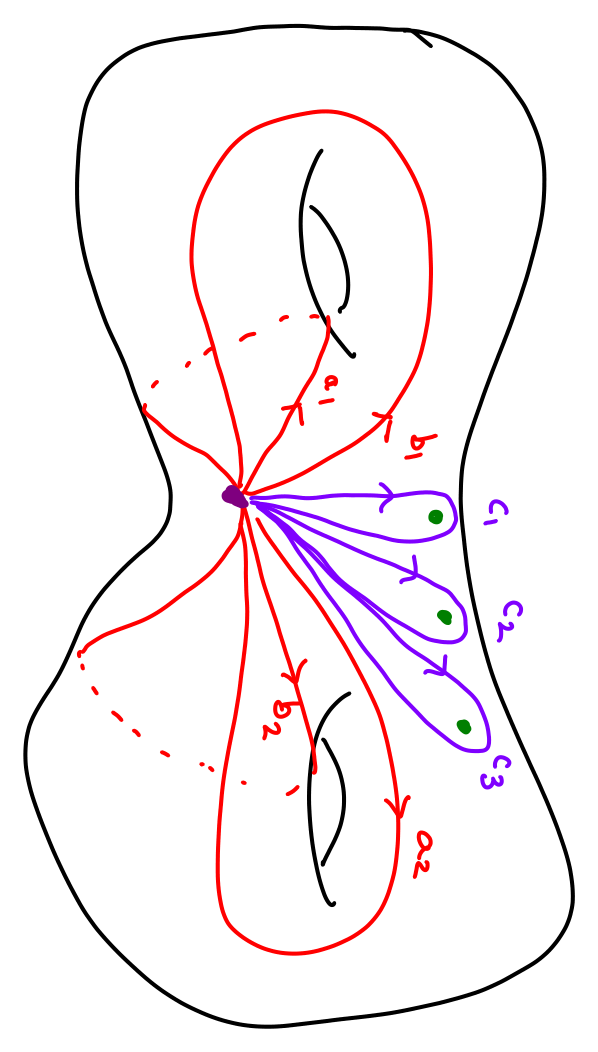
\includegraphics[width=0.6\textwidth]{figures/fig02.png}
  \caption{亏格为 2、带三个穿孔的曲面情形下，$\pi_1(\Sigma_2,x_0)$ 的一组生成元的选取。（原文 Fig.~2，第 35 页）}
  \label{fig:2}
\end{figure}

第二，在 $G$ 为阿贝尔、而 $X$ 任意的情形，同态 $\pi_1(X,x_0)\to G$ 通过同调上的一个同态分解：$H_1(X;\mathbb{Z})\to G$。这由 Stokes 定理可得：若 $\gamma-\gamma'=\partial\Sigma$，则\footnote{回忆我们的约定：当 $G$ 是环面群这一特殊情形时，我们把 $A$ 取作实形式。}

\begin{equation}
  \exp\Big[\mathrm{i}\oint_{\gamma}A\Big]\Big/\exp\Big[\mathrm{i}\oint_{\gamma'}A\Big]=\exp\Big[\mathrm{i}\int_{\Sigma}F\Big]=1
  \tag{2.112}
  \label{eq:2.112}
\end{equation}
事实上，这个论证表明：在阿贝尔情形，和乐只依赖于同调类 $[\gamma]\in H_1(\Sigma_2;\mathbb{Z})$。

于是，取 $G=U(1)$、$X=\Sigma_2$，我们便有

\begin{equation}
  \mathcal{M}_{\mathrm{flat}}=\operatorname{Hom}(H_1(\Sigma_2;\mathbb{Z}),U(1))
  \tag{2.113}
  \label{eq:2.113}
\end{equation}

现在 $\Sigma_2$ 的同调中没有挠元，故可以放心地说：

\begin{equation}
  \operatorname{Hom}(H_1(\Sigma_2;\mathbb{Z}),U(1))\cong H^{1}(\Sigma_2;\mathbb{R})/H^{1}(\Sigma_2;\mathbb{Z})
  \tag{2.114}
  \label{eq:2.114}
\end{equation}

这可以更直接地如下理解：我们可以直接解 $F=dA=0$。首先，这意味着第一 Chern 类为零，而它由 $\int_{\Sigma_2}F/2\pi=0$ 度量。

% [Tutor Note: (2.114) 用到两件事：一是泛系数定理给出 $\operatorname{Hom}(H_1(\Sigma_2;\mathbb{Z}),U(1))\cong H^1(\Sigma_2;\mathbb{Z})\otimes_{\mathbb{Z}}\mathbb{R}/\mathbb{Z}$，此处 $\Sigma_2$ 是闭曲面、同调无挠，故张量积与 $\operatorname{Hom}$ 一致；二是 $H^1(\Sigma_2;\mathbb{Z})\otimes\mathbb{R}\cong H^1(\Sigma_2;\mathbb{R})$。若换成带边或非紧的曲面，$H_1$ 的自由部分之外还要处理边界项，(2.113) 就不再是全部。另注意脚注 14 的实形式约定：$A$ 取实值，故 (2.116) 中 $\oint A$ 直接落在 $\mathbb{R}$ 上；若改用反厄米约定 $A\to-\mathrm{i}A$，则 (2.116)–(2.118) 的指数与系数都要相应补上 $\mathrm{i}$ 与 $2\pi$ 的因子。]

因此，我们可以把 $A$ 看成整体良定义的 1-形式。由于 $dA=0$，它是闭 1-形式。但我们必须商去平移 $A\to A+\omega$，其中 $\omega\in\Omega^{1}_{2\pi\mathbb{Z}}(\Sigma_2)$。所得空间就是

\begin{figure}[htbp]
  \centering
  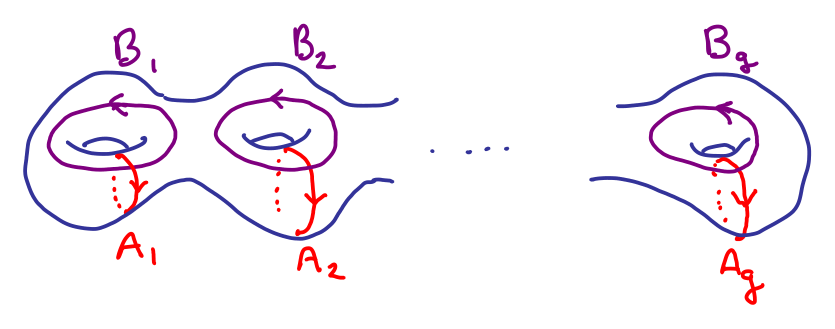
\includegraphics[width=0.55\textwidth]{figures/fig03.png}
  \caption{亏格为 $g$ 的曲面同调的一组标准基：该曲面以把手体（handlebody）表面的方式给出。（原文 Fig.~3，第 36 页；原文图注此行缺右括号，此处补全）}
  \label{fig:3}
\end{figure}

\begin{equation}
  \mathcal{M}_{\mathrm{flat}}=H^{1}(\Sigma_2;\mathbb{R})/H^{1}(\Sigma_2;\mathbb{Z})
  \tag{2.115}
  \label{eq:2.115}
\end{equation}

% 原文 (2.115) 的下标印作斜体 $flat$（(2.107)、(2.111)、(2.113)、(2.114)、(2.126) 则印作正体 $\mathrm{flat}$）；为片段内部统一，此处一律用 \mathrm{flat}。

这不过是一个 $2g$ 维的环面。若我们为同调选取显式的生成元 $A_I,B_I$（例如像图~\ref{fig:3} 那样），则有坐标

\begin{equation}
  e^{\mathrm{i}\theta_I}=e^{\mathrm{i}\oint_{A_I}A}
  \qquad\qquad
  e^{\mathrm{i}\phi_I}=e^{\mathrm{i}\oint_{B_I}A}
  \tag{2.116}
  \label{eq:2.116}
\end{equation}

在这些坐标下可以写出

\begin{equation}
  A=\theta_I\alpha_I+\phi_I\beta_I
  \tag{2.117}
  \label{eq:2.117}
\end{equation}

其中 $\alpha_I,\beta_I$ 是一次上同调类的一组对偶基，而

\begin{equation}
  \omega=\frac{\kappa}{\pi}\delta\theta_I\wedge\delta\phi_I
  \tag{2.118}
  \label{eq:2.118}
\end{equation}

% [Tutor Note: (2.118) 出现 $\kappa/\pi$ 而非环面公式里更眼熟的 $\kappa/2\pi$，原因有二：其一，辛形式取自 $\frac{\kappa}{2\pi}\int_{\Sigma_2}\delta A\wedge\delta A$，而 (2.117) 给出 $\int_{\Sigma_2}\delta A\wedge\delta A=2\,\delta\theta_I\wedge\delta\phi_I$（$\int_{A_J}\alpha_I=\delta_{IJ}$、$\int_{B_J}\beta_I=\delta_{IJ}$），因子 $2$ 把 $2\pi$ 抵消成 $\pi$；其二，$\theta_I,\phi_I$ 由 (2.116) 的 $e^{\mathrm{i}\theta_I}$ 定义，本身已是模 $2\pi$ 的坐标。用 $\{\theta_I,\phi_J\}=\frac{\pi}{\kappa}\delta_{IJ}$ 反推即可自查。另：(2.117)、(2.118) 中重复指标 $I$ 按 Einstein 约定求和，原文未显式写出 $\sum_I$。]

\textbf{注记：}

\begin{enumerate}
  \item \underline{维数公式}。警觉的读者会注意到，\eqref{eq:2.111} 有时可以是负的。确实，这是一个虚维数公式。若共轭作用在 $\operatorname{Hom}(\pi_1,G)$ 的光滑点处自由作用，它才真正给出某个流形的维数。然而，若群作用不是有效的，真实维数就不由该公式给出（如果那里还有个流形的话）。例如，考虑 $\Sigma_2$ 是不带穿孔的 $S^{2}$ 的情形。此时 $\pi_1$ 是只有一个元素的群，同态也只有一个。模叠就是叠 $pt//G$，形式上具有负维数。在接下来的几节中我们将研究 $G=U(1)$ 的环面。此时对易子方程事实上不施加任何约束，而共轭作用平凡地作用。所以真实维数是

  \begin{equation}
    2g\dim G=2\times 1\times 1=2
    \tag{2.119}
    \label{eq:2.119}
  \end{equation}

  而两个形式上的减法 $-\dim G-\dim G$ 对虚维数贡献 $-2$，也就是零。某种意义上每一点都是「奇异的」，因为除以共轭作用这件事处处都是平凡的。

  \item \underline{辛结构的内禀定义}。我们已经从 \eqref{eq:2.93} 看到，$\Sigma_2$ 上平坦规范场的空间是某个辛空间的 Hamilton 约化，因此辛形式继承自 \eqref{eq:2.79}。在阿贝尔情形把它写下来相当直接，正如我们上面所做的。在非阿贝尔情形，写出显式公式则更具挑战性。这件事在 [24, 25] 中完成了，我们这里给出简要描述。记 $\pi:=\pi_1(\Sigma_2,x_0)$。设有同态 $\phi:\pi\to G$。通过在 $\phi$ 处构造同态空间的一个切向量 $v$，人们容易看出 $v$ 应被视为一个群上循环 $\phi\in Z^{1}(\pi;\mathfrak{g}_{\mathrm{Ad}(\phi)})$。这里我们用的是系数取自 $\pi$ 的某个表示中的群上循环，该表示由 $\rho(\gamma):=\mathrm{Ad}(\phi(\gamma))$ 作用在 $\mathfrak{g}$ 上给出。为了理解这一点，设有同态族 $\phi_t:\pi\to G$，它给出在 $t=0$ 时刻经过 $\phi=\phi_0$ 的一条路径。那么，对每个 $\gamma\in\pi$ 我们都有 $G$ 中群元素的一条路径：$\phi_t(\gamma)=g_\gamma(t)$。现在定义

  \begin{equation}
    v:\pi\to\mathfrak{g}
    \tag{2.120}
    \label{eq:2.120}
  \end{equation}

  为

  \begin{equation}
    v(\gamma):=\phi(\gamma)^{-1}\frac{d}{dt}\Big|_{0}\phi_t(\gamma)=g_\gamma(0)^{-1}\frac{d}{dt}\Big|_{0}g_\gamma(t)
    \tag{2.121}
    \label{eq:2.121}
  \end{equation}

  现在我们必须施加群同态性质：

  \begin{equation}
    \phi_t(\gamma_1)\phi_t(\gamma_2)=\phi_t(\gamma_1\gamma_2)
    \tag{2.122}
    \label{eq:2.122}
  \end{equation}

  它对一切 $\gamma_1,\gamma_2\in\pi$ 成立。在 $t=0$ 处求导，并把方程左乘 $\phi_0(\gamma_1\gamma_2)^{-1}$，得到：

  \begin{equation}
    \mathrm{Ad}(\phi_0(\gamma_2))v(\gamma_1)-v(\gamma_1\gamma_2)+v(\gamma_2)=0
    \tag{2.123}
    \label{eq:2.123}
  \end{equation}
\end{enumerate}

% 跨片段引用说明：\eqref{eq:2.93} 与 \eqref{eq:2.79} 指向 c03 片段中的 (2.93)、(2.79)（平坦联络空间作为辛空间的 Hamilton 约化），其 \label 由 c03 提供，本片段不重复引入。

% [Tutor Note: 第 2 条注记里「one easily sees that $v$ should be considered as a group cocycle」这一步的实质是把「同态空间在 $\phi$ 处的切向量」认同为 $\pi$ 的 1-上循环；原文这里把上循环也记作 $\phi$（应为 $v$），与同态本身重名，读者须按 (2.121) 的定义把 $v$ 与 $\phi$ 区分开。真正的计算在 (2.122)$\to$(2.123)：对 $\phi_t(\gamma_1)\phi_t(\gamma_2)=\phi_t(\gamma_1\gamma_2)$ 求导得 $\dot\phi_t(\gamma_1)\phi_t(\gamma_2)+\phi_t(\gamma_1)\dot\phi_t(\gamma_2)=\dot\phi_t(\gamma_1\gamma_2)$，再用 $\phi_t(\gamma_1)^{-1}\dot\phi_t(\gamma_1)=v(\gamma_1)$ 把各项都化成 $v$，才得到 (2.123) 的三项式。]

这正是系数取在 $\mathfrak{g}$ 中的群上循环条件，其中 $\mathfrak{g}$ 通过 $\gamma\to\mathrm{Ad}(\phi(\gamma))$ 被看作一个 $\pi$-表示。这种上循环构成的空间记作 $Z^{1}(\pi;\mathfrak{g}_{\mathrm{Ad}(\phi)})$。另一方面，若作一族同态

\begin{equation}
  \phi_t(\gamma)=g(t)^{-1}\phi(\gamma)g(t)
  \tag{2.124}
  \label{eq:2.124}
\end{equation}

其中 $g(t)=e^{-tX}$ 是某一族，$X\in\mathfrak{g}$，那么由于我们的空间是商去 $G$ 的共轭作用而得到的，显然应当模去这类切向量。再次在 $t=0$ 处求导可知，这类切向量是

\begin{equation}
  v(\gamma)=\mathrm{Ad}(\phi(\gamma))X-X
  \tag{2.125}
  \label{eq:2.125}
\end{equation}

这正是一边上循环 $B^{1}(\pi;\mathfrak{g}_{\mathrm{Ad}(\phi)})$ 的定义。于是我们断定，存在自然的同构

\begin{equation}
  T_{[\phi]}\mathcal{M}_{\mathrm{flat}}\cong H^{1}(\pi;\mathfrak{g}_{\mathrm{Ad}(\phi)})
  \tag{2.126}
  \label{eq:2.126}
\end{equation}

现在，由于 $\Sigma_2$ 有单连通的覆叠\footnote{这就是单值化定理（uniformization theorem）：$g=0$ 时它单连通，$g=1$ 时覆叠是 $\mathbb{C}$，$>1$ 时则是上半平面，或等价地是圆盘。技术上，我们所用的条件是：只要 $\Sigma_2$ 不是不带穿孔的球面，该曲面就是 $K(\pi,1)$ 空间。}，我们可以把群上同调与奇异上同调等同起来：$H^{k}(\pi;M)\cong H^{k}(\Sigma_2;M)$。确实，若我们有平坦 $G$ 丛 $P\to\Sigma_2$，则存在伴随丛，而平坦 $G$ 丛的空间在某点的切空间是 $H^{1}(\Sigma_2;\mathrm{ad}P)$。利用 $\mathfrak{g}$ 上的迹形式，相乘并积分，我们便得到一个映射

\begin{equation}
  H^{1}(\pi;\mathfrak{g}_{\mathrm{Ad}(\phi)})\times H^{1}(\pi;\mathfrak{g}_{\mathrm{Ad}(\phi)})\to\mathbb{R}
  \tag{2.127}
  \label{eq:2.127}
\end{equation}

这就是辛形式的 Goldman 描述。描述它的一个有用方式，是用经典 Wilson 线的 Poisson 括号。一般地，若 $f:G\to\mathbb{R}$ 是 $\mathrm{Ad}$-不变函数，令 $df:G\to\mathfrak{g}$ 为由下式定义的函数

\begin{equation}
  \frac{d}{dt}\Big|_{0}f(ge^{tX})=\operatorname{tr}\big(df(g)X\big)
  \tag{2.128}
  \label{eq:2.128}
\end{equation}

那么 [25] 中证明了：若 $W_R(\gamma,A)=\operatorname{Tr}_R P\exp\oint_{\gamma}A$，则可以为这些函数的 Poisson 括号写出一个漂亮的显式公式：

\begin{equation}
  \{W_R([\gamma_1],\cdot),W_R([\gamma_2],\cdot)\}
  =\sum_{p\in\gamma_1\cap\gamma_2}\iota_p(\gamma_1,\gamma_2)\operatorname{tr}\big(dW_R(\gamma_1(p),\cdot)\,dW_R(\gamma_2(p),\cdot)\big)
  \tag{2.129}
  \label{eq:2.129}
\end{equation}

在这个公式中，我们为同伦类选取了在有限多个点上横截相交的一般位置代表元 $\gamma_1,\gamma_2$。对 $p\in\gamma_1\cap\gamma_2$，我们用 $\gamma_i(p)$ 记 $\gamma_i$ 的以 $p$ 为基点的代表元。这并不显然，但确实右端所用的代表元的选取无关紧要。

考虑到规范场上 (3.38) 的 Poisson 括号，括号 \eqref{eq:2.129} 是非常合理的：delta 函数的支集意味着只可能有来自交点的贡献。然后作一个简单的局部分析，就可以推出该公式。

% 跨片段引用：正文中的 (3.38) 指第 3 章给出的规范场 Poisson 括号（该章片段尚未译出），此处按原文以文字标注编号，待第 3 章片段就位后可改用 \eqref{eq:3.38}。

{\small\itshape ［原文标记：这件事应当详细做一遍！！本质上这正是 GMN2 的附录 B 中所做的事。］}% [原文待办标记，原文 p.38 右边栏]

% [Tutor Note: (2.129) 中「It is not obvious, but it is true that the choice of representative used on the RHS does not matter」省略的论证是：改换代表元 $\gamma_i\mapsto\eta_i^{-1}\gamma_i\eta_i$（$\eta_i$ 基于交点 $p$）只使 $dW_R$ 在 $\gamma_i(p)$ 处共轭，而 $\operatorname{tr}$ 循环不变，故右端不变；同时交点数 $\iota_p(\gamma_1,\gamma_2)=\pm1$ 的符号依赖于曲面定向与 $\gamma_1,\gamma_2$ 在 $p$ 处有序切向的夹角方向，换定向会使整个括号变号——这与 $\{\cdot,\cdot\}$ 作为辛形式之逆的定义是自洽的。原文未交代 $\iota_p$ 的符号约定，核对时须与本段的辛形式 (2.118) 定向一致。]

% 注意：本片段从第 2 章（2.2.8）中间开始，父 \section 在 c03 片段中定义
% =====================================================================
%  c05：原印刷页 39–46（PDF p.40–47）
%  §2.2.8、§2.2.9，以及 §2.2.9 内一个无编号小标题
%  （Generalization To Compact Riemann Surface Of Genus g）
%  片段开头 (2.130) 及其引导句仍属上一小节 2.2.7 的收尾（承接 c04 片段末尾，
%  勿与之重复），故此处不补任何标题；本片段无图；公式编号 (2.130)–(2.180) 连续。
% =====================================================================

对于 $f(\gamma,A)=2\operatorname{Re}\chi_{fund}(\gamma,A)$、$G=GL(n,\mathbb{R})$ 或 $GL(n,\mathbb{C})$ 的情形，上式化简为

\begin{equation}
  \{f(\gamma_1,\cdot),f(\gamma_2,\cdot)\}
  = \sum_{p\in\gamma_1\cap\gamma_2}\iota_p(\gamma_1,\gamma_2)\,f\big(\gamma_1(p)\cdot\gamma_2(p),\cdot\big)
  \tag{2.130}
  \label{eq:2.130}
\end{equation}

\subsubsection{环面上平坦联络的量子化：真实版本} % 原文: 2.2.8 Quantization Of Flat Connections On The Torus: The Real Story

我们现在把讨论具体化到 $\Sigma_2=T^2$，即二维环面。

这里我们面对的是 Chern-Simons 理论量子化中最基本、也最容易上手的例子之一。因此我们会以极其详尽——乃至令人痛苦——的细致程度来处理它。

我们把它写成 $T^2=\mathbb{R}^2/\mathbb{Z}\oplus\mathbb{Z}$，也就是取坐标 $(\sigma^1,\sigma^2)$，满足

\begin{equation}
  \sigma^i\sim\sigma^i+1 \qquad i=1,2
  \tag{2.131}
  \label{eq:2.131}
\end{equation}

$\pi_1$ 有两个生成元，我们可以取下列代表：

\begin{equation}
  \begin{aligned}
    \alpha:\quad & \gamma(t)(\sigma^1(t),\sigma^2(t))=(t,0) &\quad & 0\le t\le 1\\
    \beta:\quad & \gamma(t)(\sigma^1(t),\sigma^2(t))=(0,t) &\quad & 0\le t\le 1
  \end{aligned}
  \tag{2.132}
  \label{eq:2.132}
\end{equation}

平坦 $U(1)$ 规范场的规范等价类，由绕 $\alpha$、$\beta$ 两个圈的和乐（holonomy）描述：

\begin{equation}
  U_1=\operatorname{Hol}(\alpha)=\exp i\oint_\alpha A
  \qquad\qquad
  U_2=\operatorname{Hol}(\beta)=\exp i\oint_\beta A
  \tag{2.133}
  \label{eq:2.133}
\end{equation}

我们可以取对数：

\begin{equation}
  U_i=e^{ia_i} \qquad a_i\in\mathbb{R}/2\pi\mathbb{Z}
  \tag{2.134}
  \label{eq:2.134}
\end{equation}

用微分形式写出来，$T^2$ 上最一般的平坦 $U(1)$ 规范场是

\begin{equation}
  A=a_1d\sigma^1+a_2d\sigma^2
  \tag{2.135}
  \label{eq:2.135}
\end{equation}

其中由于大规范变换，我们必须作等同 $a_i\sim a_i+2\pi\mathbb{Z}$。为了得到正确归一的辛形式，把它代入作用量：

\begin{equation}
  \frac{\kappa}{2\pi}\int_{T^2\times\mathbb{R}}A\,dA
  =\frac{\kappa}{2\pi}\int dt\,(a_1\dot a_2-a_2\dot a_1)
  \tag{2.136}
  \label{eq:2.136}
\end{equation}

于是我们重新得到上文一般结果 {\small\itshape ［原文标记：****］} 的一个特例：
% [原文待办标记，原文 p.39：「****」是作者留作公式编号占位而始终未填的记号]

\begin{equation}
  \omega=\frac{\kappa}{\pi}da_1\wedge da_2
  \tag{2.137}
  \label{eq:2.137}
\end{equation}

\textbf{评注}

\begin{enumerate}
  \item 按我们的归一化，Hilbert 空间中半经典态数由 $\omega/(2k)$ 的辛体积给出。在本情形下即
  \begin{equation}
    \int_{\mathcal{M}_{flat}}\frac{\omega}{2\pi}=2\kappa
    \tag{2.138}
    \label{eq:2.138}
  \end{equation}
  % [Tutor Note: 这里的 $2\pi$ 要核对两处。(i) (2.137) 的系数：由 (2.136) 读出辛形式时须用 $a_1\dot a_2-a_2\dot a_1=2a_1\dot a_2-\frac{d}{dt}(a_2a_1)$，于是作用量已是 $\int dt\,p\dot q$ 的形式，$p=\frac{\kappa}{\pi}a_1$、$q=a_2$，故 $\omega=dp\wedge dq=\frac{\kappa}{\pi}da_1\wedge da_2$；若漏掉这个「因子 2」而写成 $2\kappa/\pi$，(2.138) 就会差一个因子 2，(2.148) 的 $2\kappa$ 维也无从谈起。(ii) 上一行正文印作 $\omega/(2k)$（斜体 $k$），而 (2.138) 左端是 $\omega/2\pi$：按「辛体积＝半经典态数」的标准陈述此处应为 $\omega/(2\pi)$，$k$ 极可能是 $\pi$ 的误植；若把 $k$ 当作能级（即 $\kappa$），则与 $2\kappa$ 维的结论不自洽。此处照原文转写，请以 (2.138) 为准。]

  \item 要做量子化，我们必须选定相空间上哪个坐标是「位置」、哪个是「动量」。这里显然存在歧义。经典地，我们可以对 $a_i$ 作取值于 $Sp(2,\mathbb{R})$ 的辛变换。由于 $a_i$ 的周期性条件，我们只被允许作 $Sp(2,\mathbb{Z})$ 中的变换。因此取
  \begin{equation}
    \begin{pmatrix}a_1<本地路径>
    \to A\begin{pmatrix}a_1<本地路径>
    \tag{2.139}
    \label{eq:2.139}
  \end{equation}
  其中
  \begin{equation}
    A=\begin{pmatrix}\alpha & \beta\\ \gamma & \delta\end{pmatrix}
    \in SL(2,\mathbb{Z})=Sp(2,\mathbb{Z})
    \tag{2.140}
    \label{eq:2.140}
  \end{equation}

  \item 这些正则变换也可以等同于环面的大微分同胚（large diffeomorphism）的作用。\eqref{eq:2.139}、\eqref{eq:2.140} 的变换等价于
  \begin{equation}
    \begin{pmatrix}\tilde\sigma^1\\ \tilde\sigma^2\end{pmatrix}
    =\begin{pmatrix}\delta & -\gamma\\ -\beta & \alpha\end{pmatrix}
    \begin{pmatrix}\sigma^1\\ \sigma^2\end{pmatrix}
    \tag{2.141}
    \label{eq:2.141}
  \end{equation}
  显然，这是环面的一个微分同胚。事实上，按下述意义它是一个非平凡的微分同胚：

  一般地，若 $X$ 是光滑流形，可以在 $X$ 的全部微分同胚构成的群上赋予一个拓扑。这是一个无穷维（Banach）Lie 群。单位元的连通分支是正规子群，商群 $Diff(X)/Diff_0(X)$ 常被称为大微分同胚群。\footnote{更确切地说，大微分同胚是 $Diff(X)$ 中落到商群的非平凡元素上去的那些元素。} 在环面的情形，利用与万有覆盖之间的简单关系，可以证明 $Diff^+(T^2)/Diff^+_0(T^2)\cong SL(2,\mathbb{Z})$。
  % [Tutor Note: 「显然，这是环面的一个微分同胚」与「可以证明 $Diff^+(T^2)/Diff^+_0(T^2)\cong SL(2,\mathbb{Z})$」两处都被作者一句带过。要把 (2.141) 与 (2.139)(2.140) 对上，需注意 $\tilde\sigma=\delta\sigma^1-\gamma\sigma^2$ 这类线性变换保持 $\mathbb{Z}\oplus\mathbb{Z}$ 的格，且 $A$ 与 (2.141) 中的矩阵互为转置逆的重新排列；而商群的同构则是最简单情形下的映射类群（mapping class group）计算：$\pi_0 Diff^+(T^2)=\pi_0 Diff(T^2)=SL(2,\mathbb{Z})$，可用万有覆盖 $\mathbb{R}^2$ 上保持格的作用（Nielsen 实现）来验证。作者未给证明，属省略。]

  {\small\itshape ［原文标记：$\clubsuit$这条评注现在与 2.2.12 节的材料重复了。$\clubsuit$］}
  % [原文待办标记，原文 p.40：页边批注，位于评注 3 旁]

  \item 我们稍后会讨论这些正则变换／微分同胚如何作用在理论的 Hilbert 空间上。
\end{enumerate}

眼下，让我们取 $a_2$ 为坐标，于是测度成为

\begin{equation}
  \exp\left(\frac{i\kappa}{\pi}\int dt\,a_1\dot a_2\right)
  \tag{2.142}
  \label{eq:2.142}
\end{equation}

够简单的：量子化之后我们必须有

\begin{equation}
  [\hat a_1,\hat a_2]=-i\frac{\pi}{\kappa}
  \tag{2.143}
  \label{eq:2.143}
\end{equation}

我们用可归一化的波函数 $\psi(a_2)$ 描述量子态，其动量为

\begin{equation}
  p_{a_2}=\frac{\kappa}{\pi}a_1
  \tag{2.144}
  \label{eq:2.144}
\end{equation}

但现在我们得施加周期性条件：首先，$\psi(a_2)$ 在 $a_2\sim a_2+2\pi n$、$n\in\mathbb{Z}$ 之下必须是周期的。

然而，与粒子在圆上运动的量子化非常不同的是，我们还必须有 $a_2$ 的周期性。
% [Tutor Note: 原文此处第二个「周期性」应为 $a_1$：紧接的下一段就改口说「若位置空间有周期性，则动量被量子化」，并明确以 $a_1\sim a_1+2\pi$ 为条件，推出 (2.146) 的 $\exp(-i2\kappa\hat a_2)\psi=\psi$（因为按 (2.145)，$a_1\to a_1+\alpha$ 由 $\exp(-i\frac{\kappa}{\pi}\alpha\hat a_2)$ 生成，取 $\alpha=2\pi$ 即得该式）。这是原文的笔误，译文照原文保留，读者按 $a_1$ 理解即可。]

通常，位置空间的周期性意味着动量被量子化，从而 de Broglie 波才能装进这个周期性的空间。因此我们预期，动量的周期性应当把位置量子化。

确实，如果我们改用 $a_1$ 作坐标来量子化，那么

\begin{equation}
  \hat a_2=i\frac{\pi}{\kappa}\frac{\partial}{\partial a_1}
  \tag{2.145}
  \label{eq:2.145}
\end{equation}

于是 $\exp(-i\frac{\kappa}{\pi}\alpha\hat a_2)$ 把 $a_1$ 平移为 $a_1+\alpha$；因此，若我们希望有周期性 $a_1\sim a_1+2\pi$，那么回到以 $a_2$ 为坐标、以波函数 $\psi(a_2)$ 描述态的 Schrödinger 绘景，我们必须有

\begin{equation}
  e^{-i2\kappa\hat a_2}\psi=\psi
  \tag{2.146}
  \label{eq:2.146}
\end{equation}

但是，既然我们处在以 $a_2$ 为坐标的 Schrödinger 表示中，这就意味着

\begin{equation}
  e^{-i2\kappa a_2}\psi(a_2)=\psi(a_2)
  \tag{2.147}
  \label{eq:2.147}
\end{equation}

这意味着 $\psi$ 只能支撑在由 $a_2=\frac{n\pi}{\kappa}\bmod 2\pi\mathbb{Z}$ 给出的那些 $a_2$ 值上，于是不同的可能性为 $n=0,\dots,2\kappa-1 \bmod 2\kappa$。
% [Tutor Note: 相位与整性条件是本节的两个陷阱。(i) 相位：(2.145) 的 $i$、$\exp(-i\frac{\kappa}{\pi}\alpha\hat a_2)$ 中的 $-i$、以及 (2.146) 的 $e^{-i2\kappa\hat a_2}$，三者的符号必须配套。若把 (2.145) 写成 $-i\frac{\pi}{\kappa}\partial_{a_1}$，则 $\exp(-i\frac{\kappa}{\pi}\alpha\hat a_2)$ 平移的将是 $a_1\to a_1-\alpha$，此时要得到 $a_1\to a_1+2\pi$ 就得改用 $e^{+i2\kappa\hat a_2}$（最终格点集仍是 $a_2=n\pi/\kappa$）；指数与生成元的符号若不配套，中间步骤会自相矛盾。(ii) 整性：由 (2.147) 解出 $a_2=n\pi/\kappa$ 时，要求 $n$ 与 $n+2\kappa$ 给出同一点，故 $2\kappa$ 必须是整数；这正是预量子化线丛存在的整性条件（Weyl 整性），也是 (2.148) 求和上限为 $2\kappa-1$ 的原因。$\kappa$ 半整数时态空间维数为奇数，仍自洽；若 $\kappa$ 非半整数，则整套构造不成立。]

结论：既然动量与坐标都是周期的，一般的波函数形如

\begin{equation}
  \psi=\sum_{n=0}^{2\kappa-1}\psi_n\,\delta\left(a_2-\frac{n\pi}{\kappa}\right)
  \qquad \psi_r\in\mathbb{C}
  \tag{2.148}
  \label{eq:2.148}
\end{equation}
% [Tutor Note: 两点。(i) 原文右端的 $\psi_r\in\mathbb{C}$ 应为 $\psi_n\in\mathbb{C}$（求和指标是 $n$），此处照原文转写，未改。(ii) 作者跳步：这样写出的 $\psi$ 是 $\delta$ 函数的叠加，按 $L^2$ 意义并不可归一（原文自身在页边用「DOESN'T LOOK VERY NORMALIZABLE! JUSTIFY」点出了这一点）。正确的处理是几何量子化：预量子化线丛的平方可积全纯截面空间自然是 $2\kappa$ 维的，$\delta$ 基只是「位置表象」中的形式写法；相干态基即 (2.177) 中的 $\chi_{\mu,\kappa}$。]

{\small\itshape ［原文标记：$\clubsuit$看上去并不很可归一！请说明理由。$\clubsuit$］}
% [原文待办标记，原文 p.41：(2.148) 右侧页边批注]

我们于是得出结论：环面上的态空间 $\mathcal{H}(T^2)$ 是一个维数为 $2\kappa$ 的复 Hilbert 空间。

这个问题同构于「在环的离散近似上运动的粒子」的量子化：我们把环看作 $U(1)$，而「离散近似」则是循环群 $\mathbb{Z}_{2\kappa}$ 的嵌入。

\subsubsection{环面上平坦联络的量子化：相干态版本} % 原文: 2.2.9 Quantization Of Flat Connections On The Torus: The Coherent Story

本节中我们给拓扑曲面 $\Sigma_2$ 赋予一个复结构 $J$。$(\Sigma_2,J)$ 合起来定义一张 Riemann 面。

我们仍先考虑 $\Sigma_2$ 是环面的情形，如上一节。环面上的一般复结构所给出的 Riemann 面可以写成椭圆曲线：

\begin{equation}
  (\Sigma_2,J)=E_\tau=\mathbb{C}/(\mathbb{Z}\oplus\tau\mathbb{Z})
  \tag{2.149}
  \label{eq:2.149}
\end{equation}

其中 $\tau$ 是复数，且必须有非零虚部，以使商是一个好的流形。复结构由下述说法确定：

\begin{equation}
  d\zeta=d\sigma^1+\tau d\sigma^2
  \tag{2.150}
  \label{eq:2.150}
\end{equation}

是 $(1,0)$ 形式。我们需要在 $\Sigma_2$ 上选一个定向，我们选 $d\sigma^1\wedge d\sigma^2$。

{\small\itshape ［原文标记：$\clubsuit$换个更好的字体：这里需要一个花体的 z。$\clubsuit$］}
% [原文待办标记，原文 p.41：页边批注，作者想把符号换成一个「花体的 z」，故下文由 $\zeta$ 改记为 $z$]

给定复结构后，存在一个典范定向 $id\zeta\wedge d\bar\zeta$。把它算出来就会看到，我们应当取 $\operatorname{Im}\tau>0$。

数学事实：$\tau,\tau'$ 定义等价的复结构，当且仅当

\begin{equation}
  \tau'=\frac{a\tau+b}{c\tau+d} \qquad
  \begin{pmatrix}a & b\\ c & d\end{pmatrix}\in SL(2,\mathbb{Z})
  \tag{2.151}
  \label{eq:2.151}
\end{equation}

也就是说，$E_\tau$ 与 $E_{\tau'}$ 作为复流形同构，当且仅当 \eqref{eq:2.151} 成立。于是我们得到复结构的模空间（「栈」）

\begin{equation}
  \mathcal{M}_{cplx}(\Sigma_2)\cong\mathcal{H}/SL(2,\mathbb{Z})
  \tag{2.152}
  \label{eq:2.152}
\end{equation}

{\small\itshape ［原文标记：****／Keyhole：请用两个 2 阶、3 阶轨形点来解释「stack」一词。／****］}
% [原文待办标记，原文 p.42：作者留下一段「Keyhole」待补的说明]

$\Sigma_2$ 上的复结构诱导平坦规范场空间上的复结构：

\begin{equation}
  \begin{aligned}
    A&=a_1d\sigma^1+a_2d\sigma^2\\
    &=a_\zeta d\zeta+a_{\bar\zeta}d\bar\zeta\\
    a_\zeta&=\frac{a_2-\bar\tau a_1}{\tau-\bar\tau}\\
    a_{\bar\zeta}&=-\frac{a_2-\tau a_1}{\tau-\bar\tau}
  \end{aligned}
  \tag{2.153}
  \label{eq:2.153}
\end{equation}

$a_\zeta$ 与 $a_{\bar\zeta}$ 充当平坦联络模空间上的（反）全纯坐标。

定义略微修改过的坐标其实会很有用：

\begin{equation}
  \begin{aligned}
    \tilde a_{\bar\zeta}&=(a_2-\tau a_1)/2\pi\\
    \tilde a_\zeta&=(a_2-\bar\tau a_1)/2\pi
  \end{aligned}
  \tag{2.154}
  \label{eq:2.154}
\end{equation}

因为我们希望波函数随复结构全纯地变化，而不是反全纯地变化，\footnote{更概念化的理由是：Cauchy-Riemann 算子 $\bar\partial_A$ 在复结构变化下的改变为
\begin{equation}
  \bar\partial_A\to\bar\partial_A+\mu\partial_A
  \tag{2.155}
  \label{eq:2.155}
\end{equation}
其中 $\mu$ 是 Beltrami 微分：一个 $(-1,1)$ 型的形式。闭 Beltrami 微分构成的空间可以典范地等同于 $\Sigma_2$ 上复结构空间的全纯切空间。} 我们将取 $z=\tilde a_{\bar\zeta}$。我们把它归一化，使之具有周期性

\begin{equation}
  z\sim z+n+m\tau \qquad n,m\in\mathbb{Z}
  \tag{2.156}
  \label{eq:2.156}
\end{equation}

此时 Poisson 括号为

\begin{equation}
  \{z,\bar z\}=\frac{\operatorname{Im}\tau}{2\pi i}\frac{1}{\kappa}
  \tag{2.157}
  \label{eq:2.157}
\end{equation}

并且由 \eqref{eq:2.79}，我们有
% 跨片段引用说明：\eqref{eq:2.79} 指向 c03 片段中的 (2.79)（辛形式在模空间上的表达），本片段未重复引入；单独编译本片段时该引用会显示为「??」，属预期行为。

\begin{equation}
  \begin{aligned}
    \frac{\omega}{2\pi}
    &=\frac{\kappa}{(2\pi)^2}\int_{T^2}\delta A_s\wedge\delta A_s\\
    &=\frac{\kappa}{2\pi^2}\,\delta a_1\wedge\delta a_2\\
    &=i\kappa\,\frac{dz\wedge d\bar z}{\operatorname{Im}\tau}\\
    &=(2\kappa)\frac{i}{2\pi}\partial\bar\partial K
  \end{aligned}
  \tag{2.158}
  \label{eq:2.158}
\end{equation}

其中我们定义：

\begin{equation}
  K=2\pi\frac{(\operatorname{Im}z)^2}{\operatorname{Im}\tau}
  \tag{2.159}
  \label{eq:2.159}
\end{equation}

从而

\begin{equation}
  \partial\bar\partial K=\frac{\pi}{\operatorname{Im}\tau}dz\wedge d\bar z
  \tag{2.160}
  \label{eq:2.160}
\end{equation}
% [Tutor Note: 这里有两个 $2\pi$ 需要核对。其一，(2.158) 第二行的 $\kappa/2\pi^2$ 不是笔误：它等于 (2.137) 的 $\kappa/\pi$ 再除以 $2\pi$（左边是 $\omega/2\pi$）。其二，(2.158) 末行与 (2.160) 的相容性依赖于约定 $\partial\bar\partial K\equiv(\partial_z\partial_{\bar z}K)\,dz\wedge d\bar z$；用 (2.159) 直接算得 $\partial_z\partial_{\bar z}K=2\pi/\operatorname{Im}\tau\cdot\frac12=\pi/\operatorname{Im}\tau$（因为 $(\operatorname{Im}z)^2=-(z-\bar z)^2/4$），与 (2.160) 一致，再代入末行确实回到 $i\kappa\,dz\wedge d\bar z/\operatorname{Im}\tau$。若把 $\partial\bar\partial$ 的归一化取成 $\frac{i}{2\pi}\partial\bar\partial$（Kähler 形式的习惯），(2.158) 末尾的系数 $(2\kappa)$ 就会改变，务必逐项核对。]

导出波函数的方法有很多，其中之一如下：Berezin-Toeplitz 量子化告诉我们，去找一个全纯线丛 $\mathcal{L}_\kappa\to E_\tau$，配备一个不变 Hermitian 度规

\begin{equation}
  \|s(z)\|^2=e^{-K_\kappa}|s(z)|^2
  \tag{2.161}
  \label{eq:2.161}
\end{equation}

其中在差一个 Kähler 变换的意义下，

\begin{equation}
  K_\kappa=(2\kappa)K=4\pi\kappa\frac{(\operatorname{Im}z)^2}{\operatorname{Im}\tau}
  \tag{2.162}
  \label{eq:2.162}
\end{equation}

Hilbert 空间上的内积为

\begin{equation}
  \langle\psi_1,\psi_2\rangle
  =\int_{E_\tau}e^{-K_\kappa}\psi_1^*(z)\psi_2(z)\,\frac{\omega}{2\pi}
  \tag{2.163}
  \label{eq:2.163}
\end{equation}

其中我们用了线丛的局部平凡化，从而把 $\psi_1(z)$ 与 $\psi_2(z)$ 看作局部定义的全纯函数。等价地：我们把它拉回到万有覆盖，并在 $\mathbb{C}$ 中对 $\mathbb{Z}+\tau\mathbb{Z}$ 的平移作用取一个基本域作积分。

{\small\itshape ［原文标记：$\clubsuit$内积的整体归一化因子？？？？$\clubsuit$］}
% [原文待办标记，原文 p.43：页边批注，作者对内积的整体归一化未作确定]

考虑一个基本的全纯线丛 $\mathcal{L}_\theta\to E_\tau$ 会很有用，其中我们采用度规为

于是我们可以取 $\mathcal{L}_\kappa=\mathcal{L}_\theta^{\otimes 2\kappa}$。

那么，该如何描述 $\mathcal{L}_\theta$ 的全纯截面呢？嗯，

\begin{equation}
  e^{-2\pi\frac{(\operatorname{Im}z)^2}{\operatorname{Im}\tau}}|\psi(z)|^2
  \tag{2.164}
  \label{eq:2.164}
\end{equation}

必须是良定义的。
% [排版说明：原文把 (2.164) 的度规表达式错放在「Well,」之后（上一句「where we use the metric with」被截断）。这正是一个度规：$e^{-2\pi(\operatorname{Im}z)^2/\operatorname{Im}\tau}|\psi(z)|^2$，它等于 (2.162) 在 $2\kappa=1$（即 $\kappa=1/2$，此时 $\mathcal{L}_\kappa=\mathcal{L}_\theta$）时的情形，与下文「$\mathcal{L}_\kappa=\mathcal{L}_\theta^{\otimes 2\kappa}$」相容。译文按原文语序保留该位置。]

于是我们可以把 $\psi(z)$ 提升为万有覆盖上（即复 $z$ 平面上）的整函数，然后要求在 $z\to z+a+b\tau$（$a,b\in\mathbb{Z}$）之下不变。现在，在 $z\to z+a$ 之下，$\psi(z)$ 至多只能改变一个相位，而由于它是全纯的，这个相位必须为 1。另一方面，在 $z\to z+b\tau$ 之下，一个简短的计算表明

\begin{equation}
  \begin{aligned}
    e^{-2\pi\frac{(\operatorname{Im}(z+b\tau))^2}{\operatorname{Im}\tau}}
    &=e^{-2\pi\frac{(\operatorname{Im}z)^2}{\operatorname{Im}\tau}}
    e^{2\pi ib(z-\bar z)+i\pi b^2(\tau-\bar\tau)}\\
    &:=e^{-2\pi\frac{(\operatorname{Im}z)^2}{\operatorname{Im}\tau}}
    \,e_b(z,\tau)^{-1}\,\overline{e_b(z,\tau)}^{-1}
  \end{aligned}
  \tag{2.165}
  \label{eq:2.165}
\end{equation}
% [Tutor Note: (2.165) 第二行第二个因子上有一道横线（共轭），PDF 文本层把横线丢掉了，只留下 $e_b^{-1}e_b^{-1}$ 的样子。按 (2.166) 的 $e_b(z,\tau)=e^{-i\pi b^2\tau-2\pi ibz}$，有 $e_b^{-1}=e^{i\pi b^2\tau+2\pi ibz}$、$\overline{e_b}^{-1}=e^{-i\pi b^2\bar\tau-2\pi ib\bar z}$，两者相乘恰为 $e^{2\pi ib(z-\bar z)+i\pi b^2(\tau-\bar\tau)}$；漏掉共轭就无法还原第一行。此处已按页面图像补回横线。]

其中

\begin{equation}
  e_b(z,\tau)=e^{-i\pi b^2\tau-2\pi ibz}
  \tag{2.166}
  \label{eq:2.166}
\end{equation}

再次利用全纯性排除可能多出的相位依赖，我们得知：截面到万有覆盖的提升必须是一个整函数，它是准周期的，并满足函数方程

\begin{equation}
  \psi(z+a+b\tau)=e_b(z,\tau)\psi(z) \qquad a,b\in\mathbb{Z}
  \tag{2.167}
  \label{eq:2.167}
\end{equation}

我们将记 $e_1(z,\tau)=e(z,\tau)$。这个函数方程很容易解：在 $z\to z+1$ 下的不变性意味着 $\psi(z)$ 必须有 Fourier 展开

\begin{equation}
  \psi(z)=\sum_{n\in\mathbb{Z}}\psi_n e^{2\pi inz}
  \tag{2.168}
  \label{eq:2.168}
\end{equation}

而在 $z\to z+\tau$ 下的变换则给出

\begin{equation}
  \psi_{n+1}=e^{i\pi(2n+1)\tau}\psi_n \qquad n\in\mathbb{Z}
  \tag{2.169}
  \label{eq:2.169}
\end{equation}

从而 $\psi_n=\psi_0e^{i\pi n^2\tau}$。

因此，在这个基本情形中，截面空间是一维的，它由 Riemann theta 函数张成：

\begin{equation}
  \theta(z,\tau)=\sum_{n\in\mathbb{Z}}e^{i\pi n^2\tau+2\pi inz}
  \tag{2.170}
  \label{eq:2.170}
\end{equation}

虽然我们把 $\theta(z,\tau)$ 写成了 $z$ 平面上的整函数，它也可以看作某个全纯线丛的全纯截面。

{\small\itshape ［原文标记：$\clubsuit$重复了吗？$\clubsuit$］}
% [原文待办标记，原文 p.44：页边批注]

接着我们定义与 Chern 类为 1 的主 $U(1)$ 丛相伴的复线丛

\begin{equation}
  L=(\mathbb{C}\times V)/(\mathbb{Z}\oplus\mathbb{Z})
  \tag{2.171}
  \label{eq:2.171}
\end{equation}

其中我们把 $V$ 看作 $U(1)$ 的一维表示。$\mathbb{Z}\oplus\mathbb{Z}$ 的一对生成元 $(g_1,g_2)$ 作用为

\begin{equation}
  \begin{aligned}
    g_1&:(z,\psi)\to(z+1,\psi)\\
    g_2&:(z,\psi)\to(z+\tau,e(z,\tau)\psi)
  \end{aligned}
  \tag{2.172}
  \label{eq:2.172}
\end{equation}

若取 $V_\ell$ 为 $V^{\otimes\ell}$，即 $U(1)$ 的荷 $\ell$ 表示，则我们得到

\begin{equation}
  L^{\otimes\ell}=(\mathbb{C}\times V_\ell)/(\mathbb{Z}\oplus\mathbb{Z})
  \tag{2.173}
  \label{eq:2.173}
\end{equation}

此时生成元作用为

\begin{equation}
  \begin{aligned}
    g_1&:(z,\psi)\to(z+1,\psi)\\
    g_2&:(z,\psi)\to(z+\tau,e(z,\tau)^\ell\psi)
  \end{aligned}
  \tag{2.174}
  \label{eq:2.174}
\end{equation}

因此，$L^{\otimes\ell}$ 的全纯截面满足如下恒等式：

\begin{equation}
  \begin{aligned}
    \psi(z+1)&=\psi(z)\\
    \psi(z+\tau)&=e^{-\ell\pi i\tau-2\ell\pi iz}\psi(z)
  \end{aligned}
  \tag{2.175}
  \label{eq:2.175}
\end{equation}

当 $\ell\ge 0$ 时存在整体全纯截面。当 $\ell<0$ 时没有整体全纯截面。

现在，正如我们所说，在量子化能级为 $\kappa$ 的 $U(1)$ Chern-Simons 理论时，相关的全纯线丛是 $\mathcal{L}_\theta^{2\kappa}$，因此若 $\psi(z)$ 是波函数，则

\begin{equation}
  \langle\psi_1,\psi_2\rangle
  =\int_{E_\tau}e^{-4\pi ik\frac{(\operatorname{Im}z)^2}{\operatorname{Im}\tau}}
  \psi_1^*(z)\psi_2(z)\frac{\omega}{2\pi}
  \tag{2.176}
  \label{eq:2.176}
\end{equation}
% [Tutor Note: (2.176) 的指数印作 $e^{-4\pi i k(\operatorname{Im}z)^2/\operatorname{Im}\tau}$，其中既有虚数单位 $i$，又把 $\kappa$ 写成了 $k$。对照 (2.162) 的 $K_\kappa=4\pi\kappa(\operatorname{Im}z)^2/\operatorname{Im}\tau$（实）与 (2.163) 的 $e^{-K_\kappa}$，此处应为实指数 $e^{-4\pi\kappa(\operatorname{Im}z)^2/\operatorname{Im}\tau}$：多出的 $i$ 会使被积函数变成纯相位，$2\kappa$ 维截面空间上的内积就不再是 Hermitian 的。原文疑有笔误，此处照原文转写，未改。]

该线丛有 $c_1(\mathcal{L}_\theta^{2\kappa})=2\kappa\,c_1(\mathcal{L}_\theta)=2\kappa$，因而将存在 $2\kappa$ 维的全纯截面空间。一组自然的截面基由能级 $\kappa$ 的 theta 函数 $\Theta_{\mu,\kappa}$ 给出。关于能级 $\kappa$ 的 theta 函数的更多细节见附录 D。

\textbf{评注}：这里我们假定 $\kappa>0$。若翻转 $\Sigma_2$ 的定向，那就会改变 $\mathcal{M}_{flat}$ 的定向，此时需要取 $\kappa<0$ 才有非零截面。

总之，当我们额外选定 $\Sigma_2$ 上的一个复结构 $J$ 作为附加数据时，我们就能构造 Chern-Simons 理论的物理态空间 $\mathcal{H}(\Sigma_2,J)$。在全纯量子化中，环面上物理态的一组基是

\begin{equation}
  \chi_{\mu,\kappa}(z,\tau)=\frac{\Theta_{\mu,\kappa}(z,\tau)}{\eta(\tau)}
  \qquad \mu\sim\mu+2\kappa
  \tag{2.177}
  \label{eq:2.177}
\end{equation}

$1/\eta(\tau)$ 这个因子在目前这一步完全不显然。我们将在下面讨论它。它可以通过以下方式得到：

\begin{enumerate}
  \item 沿复结构模空间作平行移动。
  \item 在「所有规范场构成的空间」的量子化中（并受 Gauss 定律约束）对波泛函 $\Psi[A]$ 作归一化。
\end{enumerate}

\textbf{重要评注}：用这种量子化方式，我们得到的态空间 $\mathcal{H}(\Sigma_2,J)$ 依赖于 $\Sigma_2$ 上的复结构 $J$。但 $J$ 并不是问题数据的一部分！在拓扑场论中，我们必须「摆脱」对 $J$ 的依赖。我们应把 $\mathcal{H}(\Sigma_2,J)$ 看作 $\mathcal{M}_{cplx}(\Sigma_2)$ 上某个向量丛的纤维。「态空间与 $J$ 无关」这一陈述，是由该丛上存在一个射影平坦联络来实现的。关于那个联络，详见下文。

{\small\itshape ［原文标记：****／应当讨论协变导数：上述 Hermitian 度规的 Chern 联络。／****］}
% [原文待办标记，原文 p.45：作者留待补写的段落]

\subsubsection*{推广到亏格 $g$ 的紧 Riemann 面} % 原文: Generalization To Compact Riemann Surface Of Genus g（原文为无编号、带下划线的小标题，故用 \subsubsection* 复刻）

相干态方法的一个优点是，它很容易推广到亏格为 $g$ 的紧定向曲面 $\Sigma_2$。

回忆相空间可以等同于 $2g$ 维环面 $\mathcal{P}=H^1(\Sigma;\mathbb{R})/H^1(\Sigma;\mathbb{Z})$。

若给 $\Sigma_2$ 一个复结构，使它成为 Riemann 面，那么正如我们上面显式描述过的环面情形，$\mathcal{M}_{flat}$ 继承一个复结构，满足

\begin{equation}
  T^{1,0}\mathcal{M}_{flat}\cong H^{0,1}(\Sigma_2)
  \tag{2.178}
  \label{eq:2.178}
\end{equation}

于是，我们的环面 $\mathcal{P}\cong(S^1)^{2g}$ 现在是一个复环面。预量子线丛 $L_k\to\mathcal{M}_{flat}$ 成为 $L_k=\mathcal{L}_\theta^{\otimes 2k}$，其中 $\mathcal{L}_\theta$ 仍是标准全纯线丛，具有一维的全纯截面空间。这属于一个一般的故事：（更多细节见附录 E。）

\begin{enumerate}
  \item 给定带整辛形式的辛格（symplectic lattice），可以典范地构造一个 Heisenberg 群，作为 $\Lambda\otimes\mathbb{R}/\Lambda$ 的 $U(1)$ 扩张。
  \item 该 Heisenberg 群是环面 $\Lambda\otimes\mathbb{R}/\Lambda$ 上的主 $U(1)$ 丛。
  \item 要表示该 Heisenberg 群，我们需要选取格的一个拉格朗日分解。
  \item 此外，若我们还有一个相容的复结构，那么由 $U(1)$ 的定义表示与 Heisenberg 群相伴的复线丛就是一个带典范联络的全纯线丛，其曲率代表 $c_1(L)$。
  \item 全纯截面可以提升到万有覆盖 $\Lambda\otimes\mathbb{R}\cong\mathbb{C}^n$，并且就复结构而言它是一个整函数。它是准周期函数，其自守因子由 Heisenberg 群的余循环决定。这就定义了基本的 theta 函数。
  \item $\mathcal{L}_\theta^{\otimes 2\kappa}$ 的全纯截面的一组基，是相对于 $\Lambda$ 的一个拉格朗日分裂而定义的能级 $\kappa$ 的 theta 函数。
\end{enumerate}

在我们的情形，辛格就是 $H_1(\Sigma;\mathbb{Z})$，辛形式由相交形式提供。（请记住：$\Sigma$ 是定向的。）于是 $\Sigma$ 上的复结构如前所述诱导 $H_1(\Sigma;\mathbb{R})$ 上的复结构。剩下的只是把机器开动起来。

非常具体地说：在 $\Sigma$ 上取 A、B 圈的一组基，以及对偶 1-形式 $\alpha_I,\beta^I$，$I=1,\dots,g$。于是存在一组调和 $(0,1)$ 形式：

\begin{equation}
  f_I:=\alpha_I+\tau_{IJ}\beta^J \qquad I=1,\dots,g
  \tag{2.179}
  \label{eq:2.179}
\end{equation}

而调和 $(1,0)$ 形式由下式张成

\begin{equation}
  \bar f_I:=\alpha_I+\bar\tau_{IJ}\beta^J \qquad I=1,\dots,g
  \tag{2.180}
  \label{eq:2.180}
\end{equation}
% [约定说明：原文把 $f_I=\alpha_I+\tau_{IJ}\beta^J$ 称作 $(0,1)$ 形式、把 $\bar f_I$ 称作 $(1,0)$ 形式，这与 (2.150) 处「$d\zeta=d\sigma^1+\tau d\sigma^2$ 是 $(1,0)$ 形式」的约定正好相反；按 (2.150) 的约定以及周期矩阵 $\tau_{IJ}$ 的通常用法，$f_I$ 应是全纯 $(1,0)$ 形式（附录 E 的 theta 函数即以此为基础）。此处照原文转写，读者按 (2.150) 的约定理解即可，勿与 2.2.9 节环面情形的 $\zeta$／$z$ 记号混用。]

% =====================================================================
%  c06：原印刷页 47–54（PDF p.48–55）
%  §2.2.10、§2.2.11，以及两节内的三个无编号小标题
%  （Hilbert Space For Quantization Of The Flat Gauge Fields / Clock And
%   Shift Matrices / Hilbert Space For Case Of General Compact Oriented Σ2）
%  片段开头「这里 τ_IJ 是 Siegel 上半空间的一个元素」承接 c05 末尾 (2.180)，
%  仍是 §2.2.9 末尾「推广到亏格 g」小节的收尾，故此处不补任何标题。
%  公式编号 (2.181)–(2.223) 连续；本片段含图 4（figures/fig04.png，原文第 53 页）。
% =====================================================================

这里 $\tau_{IJ}$ 是 Siegel 上半空间中的一个元素。\footnote{说到底，Siegel 上半空间就是虚部正定的 $g\times g$ 对称复矩阵所构成的空间。}

一旦有了周期矩阵，就可以按 (E.65) 所给出的方式直接定义能级 $\kappa$ 的 theta 函数。作为 $\Sigma$ 上平坦规范场空间上的全纯函数，Chern-Simons 波函数是这些 theta 函数的线性组合。要把对复结构的依赖正确地纳入 Chern-Simons 波函数，就稍微麻烦一些。这会让我们进到复结构模空间上行列式线丛（determinant line bundle）的截面。物理波函数空间的一组基是

\begin{equation}
  \chi_{\beta,\kappa}(z,\tau)=\frac{\Theta_{\beta,\kappa}(z,\tau)}{\operatorname{Det}\bar\partial}
  \tag{2.181}
  \label{eq:2.181}
\end{equation}

其中 $\operatorname{Det}\bar\partial$ 是行列式线丛 $\operatorname{DET}(\bar\partial)\to\mathcal{M}_{cplx}$ 的全纯截面。

{\small\itshape ［原文标记：$\clubsuit$这一点需要多得多的解释。$\clubsuit$］}
% [原文待办标记，原文 p.47：作者自注此处解释过于简略]

具体说来：

\begin{enumerate}
  \item Hilbert 空间 $\mathcal{H}(\Sigma)$ 的复维数是 $(2\kappa)^g$。
  {\small\itshape ［原文标记：$\clubsuit$在此处补一个指向第 2.2.12 节的前向引用。$\clubsuit$］}
  % [原文待办标记，原文 p.47]
  \item 计算模群在这些函数上的作用是很直接的。
  \item 模群的作用经过 $Sp(2g;\mathbb{Z})$ 分解（factor through），而且事实上整个群 $Sp(2g;\mathbb{Z})$ 都有作用，因为 $Sp(2g;\mathbb{Z})$ 正是辛环面的辛自同构群。
  \item 高亏格的 theta 函数也有热方程的类比（原文此处引用编号缺失，印作 (??)）。
  % [原文此处 (??) 为未解析的交叉引用，原稿即如此]
\end{enumerate}

\subsubsection{环面上平坦联络的量子化：Landau 的故事} % 原文: 2.2.10 Quantization Of Flat Connections On The Torus: Landau's Story

我们还可以用一种有趣地不同的方式得到这些结果：用第 2.2.3 节所描述的、非拓扑的有质量 Chern-Simons 理论。

这里我们遵循 [26] 的做法。这一方法对于描述 AdS/CFT 对应中的 singleton（单态）自由度 [26, 8]，以及描述 M5-膜与 M 理论 C-场（C-field）的某些拓扑侧面 [45]，都非常有用。我们在这里把一般的故事作了若干简化。关于 Maxwell-Chern-Simons 理论（包括其 $p$-形式推广）完全一般的量子化，见 [20] 第 6 节。

在眼下的理论中，由于方程是线性的，运动方程解的空间（这些解不一定彼此规范等价）是一个乘积

\begin{equation}
  S=S_f\times S_{nf}
  \tag{2.182}
  \label{eq:2.182}
\end{equation}

其中 $S_f$ 是平坦解 $F=0$ 构成的空间。它们正是拓扑扇区的解。我们可以作分解 $A=A_f+A_{nf}$，其中 $A_{nf}$ 与平坦子空间正交，例如在 Hodge 度规下正交。

{\small\itshape ［原文标记：$\clubsuit$把记号从 $X$ 改成 $\Sigma_2$。本小节中的 $k$ 也要改成 $\kappa$！！！$\clubsuit$］}
% [原文待办标记，原文 p.47：作者要求统一记号，正文未改；译文照印 X 与 k]
% [Tutor Note: 这条标记是核对系数的关键线索。作者要求把本小节的 $k$ 改记为 $\kappa$（即别处 §2.2 的能级），但两处的归一化其实并不一致：把 (2.188) 的 $\omega_f=\int_X2\pi k\,\delta A\wedge\delta A$ 与第 2.2.8 小节的 (2.137) $\omega=\frac{\kappa}{\pi}da_1\wedge da_2$ 都约化到 $T^2$ 上（取 $A=a_1d\sigma^1+a_2d\sigma^2$，则 $\int_{T^2}\delta A\wedge\delta A=2\delta a_1\wedge\delta a_2$），得 $4\pi k\,\delta a_1\wedge\delta a_2=\frac{\kappa}{\pi}\delta a_1\wedge\delta a_2$，即 $k=\kappa/4\pi^2$。所以千万不要把 (2.183) 的 $2\pi k$ 直接当成 (2.136) 里的 $\kappa/2\pi$：跨小节搬用 $2\kappa$ 维数、$\frac{2\pi i}{2\kappa}$ 相位之前，先由 (2.183) 的 $2\pi k\epsilon^{ij}A_j$ 定标，否则会差出 $4\pi^2$。同理，上面条目 1 的 $(2\kappa)^g$ 也依赖于这一能级约定。]

让我们在形如 $X\times\mathbb{R}$ 的时空上把 Hamilton 形式写出来，度规为 $-dt^2+g_{ij}dx^idx^j$，定向为 $dtdx^1dx^2$。正则共轭动量（作为矢量密度）是（取 $\epsilon^{12}=+1$）：

\begin{equation}
  \Pi^i=\frac{1}{e^2}\sqrt{g}g^{ij}(\dot A_j-\partial_jA_0)+2\pi k\epsilon^{ij}A_j
  \tag{2.183}
  \label{eq:2.183}
\end{equation}

我们得到 Hamilton 密度

\begin{equation}
  \mathcal{H}=\frac{e^2}{2\sqrt{g}}g_{ij}E^iE^j+\frac{1}{2e^2}F\wedge *_2F
  \tag{2.184}
  \label{eq:2.184}
\end{equation}

其中 $*_2$ 是 $X$ 上的 Hodge 星号，并且

\begin{equation}
  E^i:=\Pi^i-2\pi k\epsilon^{ij}A_j
  \tag{2.185}
  \label{eq:2.185}
\end{equation}

（我们也会记 $E^i=\tilde\Pi^i$。）Gauss 定律是：

\begin{equation}
  \partial_i\Pi^i+2\pi k\epsilon^{ij}\partial_iA_j=0
  \tag{2.186}
  \label{eq:2.186}
\end{equation}

如果我们「在上方」（upstairs）以 $A_0=0$ 规范来表述该理论，那么相空间的坐标是 $(\Pi^i,A_i)$，辛形式为：

\begin{equation}
  \omega=\int_X\delta\Pi^i\wedge\delta A_i
  \tag{2.187}
  \label{eq:2.187}
\end{equation}

其中 $\delta$ 是无穷维相空间上的外微分。注意，当 (2.187) 被限制到平坦规范场的子空间上时，我们会得到第二类约束，而相空间就是 Chern-Simons 辛形式

\begin{equation}
  \omega_f=\int_X2\pi k\,\delta A\wedge\delta A
  \tag{2.188}
  \label{eq:2.188}
\end{equation}

它在子空间 $F=0$ 上是规范不变的，于是可以作 Hamiltonian 约化。

{\small\itshape
［原文标记：\\
*****************************************\\
这并不完全正确！正确的版本见文献 [20]\\
*****************************************］}
% [原文待办标记，原文 p.49：作者用星号框出对上面这段推导的更正声明]
% [Tutor Note: 这个星号框针对的正是 (2.187)→(2.188) 这一步。把 (2.183) 的动量代入 (2.187)，在平坦子空间上起作用的是 $2\pi k\epsilon^{ij}A_j$ 这一项（其余部分正是被第二类约束消掉的方向），得到 $\int_X2\pi k\,\epsilon^{ij}\delta A_j\wedge\delta A_i$；按 $\epsilon^{12}=+1$ 逐项展开有 $\epsilon^{ij}\delta A_j\wedge\delta A_i=-2\,\delta A_1\wedge\delta A_2$，而 (2.188) 的 $\delta A\wedge\delta A$ 展开是 $+2\,\delta A_1\wedge\delta A_2$，两者相差一个整体符号（符号由 $\epsilon^{ij}$ 的上下标位置、$dx^1dx^2$ 与 $X$ 的定向约定共同决定）。定标的最快办法仍是回到环面：把 $\omega_f$ 与第 2.2.8 小节的 (2.137) 对齐，即可同时定下符号与 $2\pi$ 因子。作者说正确版本见 [20]，指的是那里对含 $p$-形式 Maxwell-Chern-Simons 理论做了协变相空间处理。]

重新考察 $e^2\to\infty$ 极限是很有启发的。利用 (2.184)，我们看到：若限制到有限能量的场位形，则必须令 $E^i=0$。于是由 Gauss 定律必须取 $F=0$。如我们所说，限制到这个子空间会强加第二类约束，而我们正是在限制到相空间的平坦因子。

如果我们在相空间上量子化、然后再施加 Gauss 定律，则我们有波泛函 $\Psi[A_i]$，并且用辛形式 (2.187) 来量子化。因此

\begin{equation}
  \Pi^i=-i\frac{\delta}{\delta A_i}
  \tag{2.189}
  \label{eq:2.189}
\end{equation}

由于我们可以把 $A$ 分解为 $A=A_f+A_{nf}$，而 Hamiltonian 不混合这两部分，理论的 Hilbert 空间自然可以看作乘积

\begin{equation}
  H=H_f\otimes H_{nf}
  \tag{2.190}
  \label{eq:2.190}
\end{equation}

其中 $H_f$ 是平坦势的波函数空间。

Gauss 定律是：

\begin{equation}
  \Psi(A+\omega)=e^{-2\pi ik\int\omega\wedge A}\Psi(A)
  \tag{2.191}
  \label{eq:2.191}
\end{equation}

这对大规范变换同样成立。\footnote{这需要解释。恰当的数学表述是：把 $\Psi$ 看作 $X$ 上规范势空间 $\mathcal{A}(X)$ 上某个线丛的截面。然后我们提升群作用，发现只有当 $c_1(P)=0$ 时提升才存在。在这种情形下，该线丛有典范的平凡化，也有典范联络，于是波函数成为一个函数。对于更微妙的 M 理论 C-场情形，有类似的讨论 [16]。} 这里 $\omega$ 是周期为整数的闭 1-形式。注意这并不影响 $A_{nf}$ 变量。

我们将通过在实心环面上考虑该理论的欧几里得路径积分，再把该路径积分解释为沿径向的 Hamilton 演化，来确定 singleton 的 Hamiltonian。

由于我们的作用量在导数上是二阶的，在实心环面上表述路径积分时，我们应当指定边界 $X$ 上 $A_X$ 的全部分量。这与 Chern-Simons 路径积分形成对照：后者是相空间路径积分，其中我们只指定边界 $X$ 上 $A_X$ 的一个分量。

让我们考虑该理论在半径为 $\rho$ 的实心环面 $Y_\rho$ 上的欧几里得配分函数。我们假定环面的度规在渐近上表现为 $d\rho^2+\Omega^2(\rho)g_X$。路径积分定义一个态 $\Psi_{Y_\rho}(A)$，它由下式定义

\begin{equation}
  \Psi_{Y_\rho}(A)=\int\frac{dA_Y}{\operatorname{vol}\big(\mathcal{G}(Y)\big)}\,
  e^{-\int\frac{1}{2e^2}dA*dA+2\pi ik\int AdA}
  \tag{2.192}
  \label{eq:2.192}
\end{equation}

其中 $\mathcal{G}(Y)$ 是 $Y_\rho$ 上的规范群。仅凭上面关于谱的理解，我们就能明白 $\rho\to\infty$ 时的行为。

我们可以把向大 $\rho$ 的演化看作沿欧几里得时间方向的演化。大 $\rho$ 的行为投影到最低能量的态上。

\begin{equation}
  \lim_{\rho\to\infty}\Psi_{Y_\rho}(A)=e^{-\rho\,2\pi|k|e^2}\Psi_0
  \tag{2.193}
  \label{eq:2.193}
\end{equation}

其中 $\Psi_0$ 位于环面上的基态空间之中。插入 Wilson 线之类的局部算符或其他扰动，会在这个基态空间内部引起态矢量之间的跃迁。
% [Tutor Note: 指数里 $e^2$ 在分子上，即 $e^{-\rho\,2\pi|k|e^2}$，不是 $e^{-\rho\,2\pi|k|/e^2}$（放大原文 p.50 可确认）。这与「基态能量密度为 $2\pi|k|e^2$」相符：指数应为（能量密度）×（体积）$\sim\rho$，故必与 $e^2$ 成正比。若误抄成分母，则 $e^2\to\infty$ 极限会把所有态都留下，与上文「大 $\rho$ 投影到最低能态」直接矛盾——这恰是检验此处抄写是否正确的快速判据。]

\subsubsection*{平坦规范场量子化中的 Hilbert 空间} % 原文: Hilbert Space For Quantization Of The Flat Gauge Fields（原文为无编号小标题，故用 \subsubsection* 复刻）

现在考虑在 $T^2\times\mathbb{R}$ 上的量子化。我们的波函数是 $\Psi(A_f)\otimes\Psi(A_{nf})$。非平坦扇区的谱是清楚的，我们取该因子唯一的基态波函数：它就是 [15, 14] 所描述的有质量标量的各振子的谐振子基态之乘积。本小节中我们丢掉这个因子，以便专注于对 $A_f$ 的依赖。

为简单起见，我们在环面 $X=T^2$ 上工作，取 $z=\sigma^1+\tau\sigma^2$、度规 $\Omega^2|dz|^2$、$\sigma^i\sim\sigma^i+1$。我们通过假定 $A_f$ 为常数来固定小规范变换。

在复坐标 $A=A_zdz+A_{\bar z}d\bar z$ 下，我们有

\begin{equation}
  \begin{aligned}
    \tilde\Pi^{z}&=-i\left(\frac{\partial}{\partial A_z}-4\pi k\operatorname{Im}\tau\,A_{\bar z}\right)\\
    \tilde\Pi^{\bar z}&=-i\left(\frac{\partial}{\partial A_{\bar z}}+4\pi k\operatorname{Im}\tau\,A_z\right)
  \end{aligned}
  \tag{2.194}
  \label{eq:2.194}
\end{equation}

于是 Hamilton 密度为：

\begin{equation}
  \mathcal{H}=\frac{e^2}{4\operatorname{Im}\tau}
  \big(\tilde\Pi^{z}\tilde\Pi^{\bar z}+\tilde\Pi^{\bar z}\tilde\Pi^{z}\big)
  \tag{2.195}
  \label{eq:2.195}
\end{equation}

注意它们并不对易：$[\tilde\Pi^{z},\tilde\Pi^{\bar z}]=-8\pi k\operatorname{Im}\tau$。基态能量密度为 $2\pi|k|e^2$，而且是无穷重简并的，正如标准的 Landau 能级问题那样。

若 $k>0$，我们有

\begin{equation}
  \tilde\Pi^{\bar z}\Psi=0\ \Rightarrow\ \Psi=e^{-4\pi k\operatorname{Im}\tau\,A_zA_{\bar z}}\psi(A_z)
  \tag{2.196}
  \label{eq:2.196}
\end{equation}

若 $k<0$，我们有

\begin{equation}
  \tilde\Pi^{z}\Psi=0\ \Rightarrow\ \Psi=e^{4\pi k\operatorname{Im}\tau\,A_zA_{\bar z}}\psi(A_{\bar z})
  \tag{2.197}
  \label{eq:2.197}
\end{equation}

其中 $\psi$ 是全纯的。事实上，若取 $\psi=\psi_\lambda$，其中

\begin{equation}
  \psi_\lambda(x):=e^{\lambda x}
  \tag{2.198}
  \label{eq:2.198}
\end{equation}

那么波函数集合 $\{\Psi_\lambda\mid\lambda\in\mathbb{C}\}$ 是一个张成最低 Landau 能级的超完备集。
% [Tutor Note: 这两式的共轭结构极易抄错。$k>0$ 时用 $\tilde\Pi^{\bar z}\Psi=0$，得到高斯型因子 $e^{-4\pi k\operatorname{Im}\tau A_zA_{\bar z}}$ 配上全纯的 $\psi(A_z)$；$k<0$ 时方程与函数都换成「另一侧」：$\tilde\Pi^{z}\Psi=0$、因子变为 $e^{+4\pi k\operatorname{Im}\tau A_zA_{\bar z}}$、$\psi$ 变为反全纯的 $\psi(A_{\bar z})$。注意第二个指数里 $k<0$，故 $4\pi k\operatorname{Im}\tau$ 仍是负的，两种情形下 $|A|\to\infty$ 时才都衰减——这是核对上下标与符号的最省事办法（可代 $k=-1$ 验证）。]

由 (2.198) 张成的态集合是无穷维的；但当我们考虑环面上规范不变的波函数时，LLL 就变成有限维的了。我们已经通过把平坦联络取为环面上的常数，强制了小规范变换下的不变性。我们可以通过对大规范变换取平均来施加大规范变换下的不变性。给定\emph{任意}波函数 $\Psi(A)$，其平均

\begin{equation}
  \overline{\Psi}(A):=\sum_{\omega\in\mathcal{H}^1_{\mathbb{Z}}}\Psi(A+\omega)\,e^{2\pi ik\int\omega A}
  \tag{2.199}
  \label{eq:2.199}
\end{equation}

其中 $\mathcal{H}^1_{\mathbb{Z}}$ 是周期为整数的调和 1-形式，则它按 Gauss 定律 (2.191) 变换。

如果我们考虑由形如 (2.199) 的表达式所张成的 $A_z$ 的函数空间，其中取 LLL 中的函数作为试探函数，那么由于 LLL 是无穷维矢量空间，我们起初会以为由 $\overline{\Psi}(A)$ 张成的波函数矢量空间也是无穷维的。毕竟 (2.198) 中的 $\lambda$ 可以是任意复数。然而，应用 Poisson 求和公式并作一点代数运算，我们发现（这里假定 $k>0$）：

\begin{equation}
  \overline{\Psi}_\lambda
  =e^{-4\pi k\operatorname{Im}\tau\left(A_zA_{\bar z}+A_z^2\right)-\frac{\lambda^2}{16\pi k\operatorname{Im}\tau}}
  \sqrt{\frac{\tau_2}{k}}\sum_{0\le\mu<2k}
  \Theta_{-\mu,k}\big(-2i\tau_2A_z,-\bar\tau\big)\,
  \Theta_{\mu,k}\Big(\frac{-\lambda}{4\pi ik},\tau\Big)
  \tag{2.200}
  \label{eq:2.200}
\end{equation}
% [Tutor Note: 从 (2.199) 到 (2.200) 之间，作者只说「应用 Poisson 求和公式和一点代数」，省掉的正是对 $\omega\in\mathcal{H}^1_{\mathbb{Z}}\cong\mathbb{Z}^2$ 作 Poisson 重求和：重求和把 $\Psi(A+\omega)$ 在格上的和变成对偶格上的和，即 $\mu$ 的有限和（$0\le\mu<2k$），于是无穷维的 LLL 被压成 $2k$ 维。核对时注意两个 theta 函数的模参数不是同一个：第一个用 $-\bar\tau$、第二个用 $\tau$；宗量分别是 $-2i\tau_2A_z$ 与 $-\lambda/(4\pi ik)$。若不放心，可用 (2.201) 的归一化因子 $k^{3/4}/\bar\eta$ 反推 (2.200) 的指数（$\bar\eta$ 说明这里用的是反全纯的模参数），比重新做一遍 Poisson 求和快得多，详见 [17, 26]。]

这个公式表明，作为 $A_z$ 的函数，我们只得到一个有限维空间。事实上可以证明（见 [17, 26]），平坦规范场扇区的一组归一化波函数基是：

\begin{equation}
  \psi_\mu=\frac{k^{3/4}}{\bar\eta}\,
  e^{-4\pi k\operatorname{Im}\tau\left(A_zA_{\bar z}+A_z^2\right)}
  \Theta_{-\mu,k}\big(-2i\tau_2A_z,-\bar\tau\big)
  \tag{2.201}
  \label{eq:2.201}
\end{equation}

\subsubsection{环面上平坦联络的量子化：Heisenberg 的故事} % 原文: 2.2.11 Quantization Of Flat Connections On The Torus: Heisenberg's Story

万一你对刚才得到的结果还不够放心，让我们从 Heisenberg 群的观点来看一看。

经典地，和乐由 $U_i=\exp[ia_i]$ 描述。量子地，我们得到算符：

\begin{equation}
  \widehat{U}_i=\exp[i\hat a_i]
  \tag{2.202}
  \label{eq:2.202}
\end{equation}

由对易子 \eqref{eq:2.143} 可得

\begin{equation}
  \widehat{U}_1\widehat{U}_2=e^{\frac{2\pi i}{2\kappa}}\widehat{U}_2\widehat{U}_1
  \tag{2.203}
  \label{eq:2.203}
\end{equation}

特别地，

\begin{equation}
  \widehat{U}_1\widehat{U}_2\widehat{U}_1^{-1}=e^{\frac{2\pi i}{2\kappa}}\widehat{U}_2
  \tag{2.204}
  \label{eq:2.204}
\end{equation}

这意味着 $U_1$ 把 $a_2$ 平移 $2\pi/2\kappa$，类似地 $U_2$ 平移 $a_1$。因此我们还有如下关系：

\begin{equation}
  \widehat{U}_1^{2\kappa}=\widehat{U}_2^{2\kappa}=1
  \tag{2.205}
  \label{eq:2.205}
\end{equation}

(2.204) 与 (2.205) 定义了一个有限非阿贝尔群，称为有限 Heisenberg 群。一般地，对任意整数 $N$，存在一个阶为 $N^3$ 的 Heisenberg 群。它处于一个（非分裂的）正合列中

\begin{equation}
  1\to\mathbb{Z}_N\to\mathrm{Heis}_N\to\mathbb{Z}_N\oplus\mathbb{Z}_N\to 0
  \tag{2.206}
  \label{eq:2.206}
\end{equation}

它是量子力学中通常的 Heisenberg 关系的有限群类比。

有一个标准定理，即 Stone-von Neumann 定理，它说：在同构意义下，Heisenberg 群的酉不可约表示是唯一的，其中 $U(1)$ 中的标量就简单地作用为乘以该标量。对所有 Heisenberg 群这都是对的，因此 $\mathrm{Heis}_N$ 有唯一的不可约表示。
% [Tutor Note: 作者这句话省掉了 SvN 定理的两个前提：(i) 表示须以给定的中心特征（central character）$\chi:U(1)\to U(1)$ 作用，定理说的唯一性是「在该中心特征给定之后」；(ii) 群律里的 2-上闭链（即 (2.203) 的相位）须与给定的辛形式/相交形式相容。证明只是 Schur 引理加维数计数：不可约表示的维数平方等于中心 $\mathbb{Z}_N$ 的大小 $N^2$，故维数必为 $N$；有限 Heisenberg 群的这一结论与连续情形（Stone-von Neumann 唯一性定理）是同一件事的两种版本。译者取舍：「representation」在本段既指 $U(1)$ 的电荷 $n$ 表示（纤维上的作用），又指 Heisenberg 群在 Hilbert 空间上的表示，二者都译作「表示」；缩写 SvN 保留（后文 (2.223) 处作者自己就写 SvN）。]

\subsubsection*{钟矩阵与移位矩阵} % 原文: Clock And Shift Matrices（原文为无编号小标题，故用 \subsubsection* 复刻）

呈现 Heisenberg 群 $\mathrm{Heis}_N$ 的 Stone-von Neumann 表示的一种标准方式，是通过 $N\times N$ 的「钟」（clock）矩阵与「移位」（shift）矩阵 $P$ 与 $Q$。为定义它们，引入一个 $N$ 次单位根，比如 $\omega=\exp[2\pi i/N]$。于是

\begin{equation}
  P_{i,j}=\delta_{i=j+1\operatorname{mod}N}
  \tag{2.207}
  \label{eq:2.207}
\end{equation}

\begin{equation}
  Q_{i,j}=\delta_{i,j}\omega^{j}
  \tag{2.208}
  \label{eq:2.208}
\end{equation}

注意 $P^N=Q^N=1$，且没有更小的幂等于 1。进而注意\footnote{检查这一点——从而检查你的约定是否在掌控之中——最快的办法是计算 $QPQ^{-1}$，因为 $(Q^{-1}PQ)_{ij}=Q_{ii}P_{ij}(Q_{jj})^{-1}=\omega P_{ij}$。}

\begin{equation}
  QP=\omega PQ
  \tag{2.209}
  \label{eq:2.209}
\end{equation}

当 $N=4$ 时，这两个矩阵形如

\begin{equation}
  P=
  \begin{pmatrix}
    0&0&0&1\\
    1&0&0&0\\
    0&1&0&1\\
    0&0&1&0
  \end{pmatrix}
  \qquad\qquad
  Q=
  \begin{pmatrix}
    \omega&0&0&0\\
    0&\omega^2&0&0\\
    0&0&\omega^3&0\\
    0&0&0&1
  \end{pmatrix}
  \tag{2.210}
  \label{eq:2.210}
\end{equation}

其中 $\omega=e^{2\pi i/4}$。由 $P,Q$ 生成的矩阵群是 $GL(N,\mathbb{C})$ 的一个有限子群，同构于一个有限 Heisenberg 群。在量子化一个在群 $U(1)$ 上运动、但被限制在 $N$ 阶循环子群内的量子粒子时，人们自然会遇到它们。
% [Tutor Note: 印出的 $P$ 第三行「$0\ 1\ 0\ 1$」含两个 1，不是置换矩阵，此时 $P^N=1$（更不必说「没有更小的幂等于 1」）并不成立：由 $Pe_4=e_1+e_3$ 可见 $P$ 会把某些向量越打越长。按 (2.207) 的定义 $P_{i,j}=\delta_{i=j+1\bmod N}$（$j=1,\dots,N$），$N=4$ 时应为 $(0\,0\,0\,1),(1\,0\,0\,0),(0\,1\,0\,0),(0\,0\,1\,0)$。旁证：$Q$ 的印出值 $\mathrm{diag}(\omega,\omega^2,\omega^3,1)$ 与 (2.208) 的 $Q_{i,j}=\delta_{i,j}\omega^j$ 完全一致，说明索引确从 $j=1$ 取到 $N$。此处照印未改，使用时请以定义 (2.207) 为准。]

{\small\itshape ［原文标记：$\clubsuit$关于这一点能给更多细节吗？$\clubsuit$］}
% [原文待办标记，原文 p.52：作者自注此处（U(1) 上粒子的量子化）解释不足]

\textbf{评注}：由 $P,Q$ 生成的算符代数是完整的矩阵代数 $\mathrm{Mat}_{N\times N}(\mathbb{C})$。也就是说，态空间上的任意线性变换都可以写成乘积 $P^mQ^n$ 的线性组合。

{\small\itshape ［原文标记：$\clubsuit$也许该多说说如何用有限 Fourier 变换来做这件事。$\clubsuit$］}
% [原文待办标记，原文 p.52]

\subsubsection*{一般紧定向曲面 $\Sigma_2$ 情形的 Hilbert 空间} % 原文: Hilbert Space For Case Of General Compact Oriented Σ2（原文为无编号小标题，故用 \subsubsection* 复刻）

{\small\itshape ［原文标记：$\clubsuit$为了与前面一致、并区分路径积分中插入的线缺陷与 Hilbert 空间上的算符，或许该给这些算符 $\widehat{W}(n,\gamma)$ 都加个帽子。$\clubsuit$］}
% [原文待办标记，原文 p.53：正文中确实混用了带帽与不带帽的写法]

我们可以轻而易举地把上面的讨论推广到一般紧定向曲面 $\Sigma_2$：若 $\gamma\subset\Sigma_2$ 是一条定向闭圈，$V_n$ 是 $U(1)$ 的电荷 $n$ 表示，$n\in\mathbb{Z}$，则可以构造 Wilson 线算符 $W(n,\gamma)=\exp[in\oint_\gamma A]$，见 \eqref{eq:2.61}。由于规范场是平坦的，它（在没有其他算符的情况下）只依赖于 $\gamma$ 的\underline{同调类}。特别地，相当平凡地

\begin{equation}
  \exp\Big[in\oint_\gamma A\Big]=\exp\Big[i\oint_{n\gamma}A\Big]
  \tag{2.211}
  \label{eq:2.211}
\end{equation}

有相应的量子算符。我们可以把它们写成：

\begin{equation}
  \widehat{W}(n,\gamma):=\exp\Big[in\oint_\gamma\widehat{A}\Big]
  \tag{2.212}
  \label{eq:2.212}
\end{equation}

同样，这个算符只依赖于乘积，所以我们可以简化，只用一个单变量 $\gamma\in H_1(\Sigma_2;\mathbb{Z})$ 的算符值函数 $\widehat{W}(\gamma)$ 来工作。

这些算符依赖于 $\gamma$ 的定向，并且我们有

\begin{equation}
  \widehat{W}(-\gamma)=\widehat{W}(\gamma)^{\dagger}=\widehat{W}(\gamma)^{-1}
  \tag{2.213}
  \label{eq:2.213}
\end{equation}

那么 (2.204) 的推广要用 Baker-Campbell-Hausdorff 公式以及 (2.87) 的对易子。结果是

\begin{equation}
  \widehat{W}(\gamma_1)\widehat{W}(\gamma_2)
  =e^{\frac{2\pi i}{2\kappa}I(\gamma_1,\gamma_2)}
  \widehat{W}(\gamma_2)\widehat{W}(\gamma_1)
  \tag{2.214}
  \label{eq:2.214}
\end{equation}

其中

\begin{equation}
  I(\gamma_1,\gamma_2)=\sum_{p\in\gamma_1\cap\gamma_2}\iota_p(\gamma_1,\gamma_2)
  \tag{2.215}
  \label{eq:2.215}
\end{equation}

是 $\gamma_1$ 与 $\gamma_2$ 的定向相交数。

\begin{figure}[htbp]
  \centering
  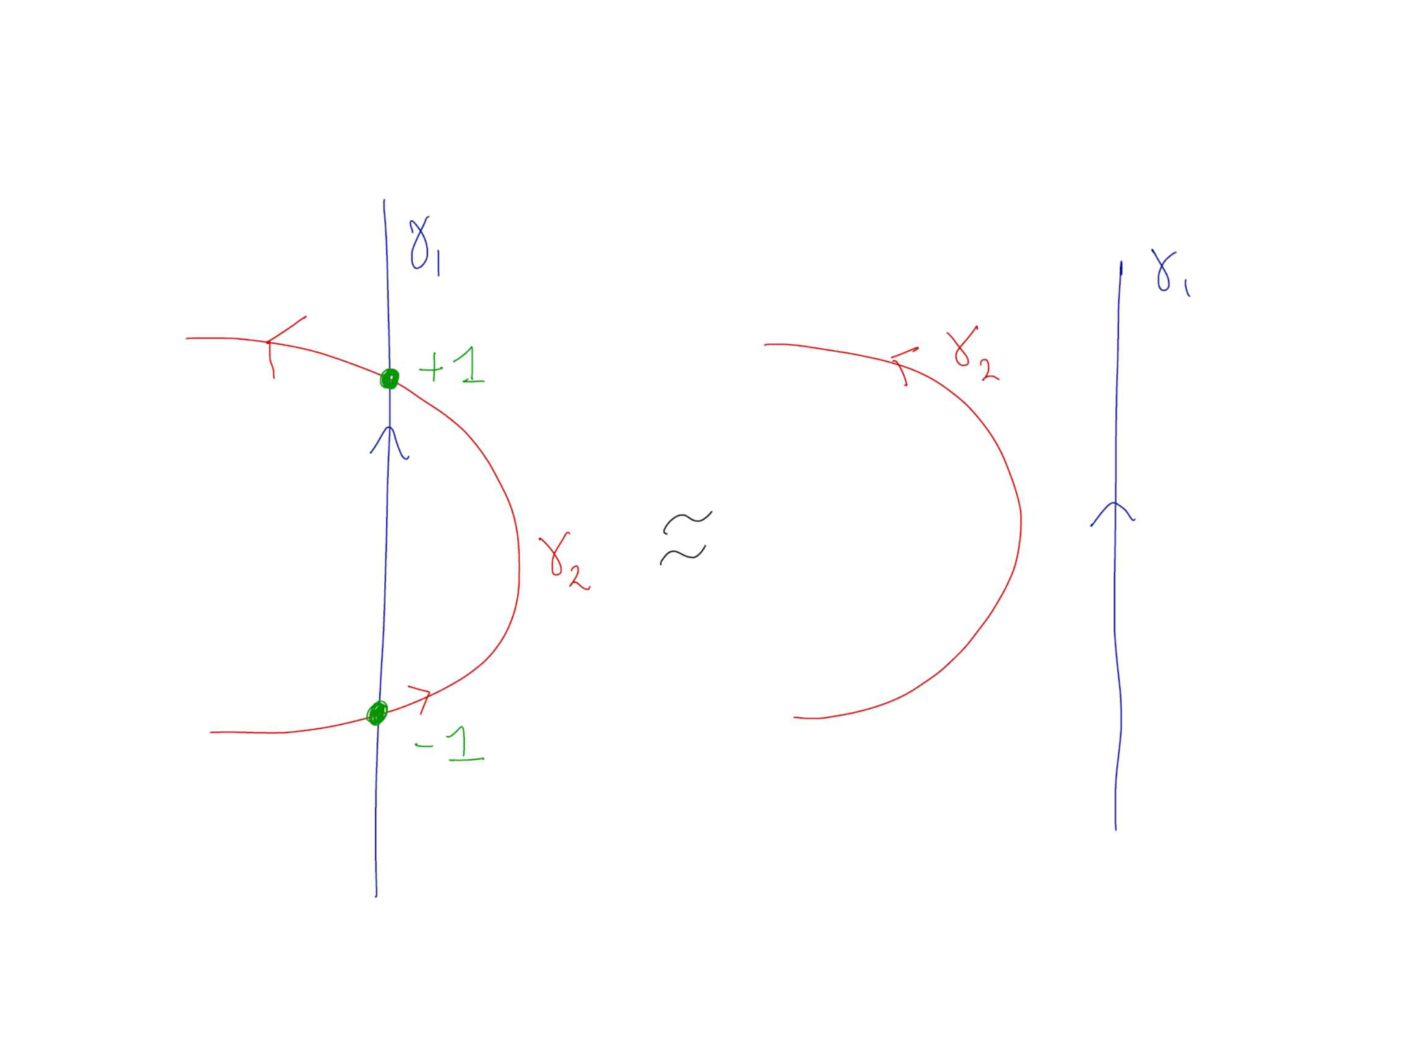
\includegraphics[width=0.78\textwidth]{figures/fig04.png}
  \caption{由于相交数是有符号的求和，其符号由定向决定，总的相交数在形变下不变，此处以一个简单情形加以说明。对横截相交的曲线求定向交点之和，给出一个只依赖于这些曲线的同调类的不变量。（原文 Fig.~4，第 53 页）}
  \label{fig:4}
\end{figure}
% [原文图注的英文原句有笔误：「with the sign determined by the orientation to total intersection number is invariant」应为「...by the orientation, the total intersection number is invariant」；此处按文意译出，未增删内容。]

为定义定向相交数，我们假定 $\gamma_1$ 与 $\gamma_2$ 处于一般位置（general position），从而交点只有有限多个，且都是横截的。于是，在每个交点 $p\in\gamma_1\cap\gamma_2$ 处，切矢量 $\{\dot\gamma_1(p),\dot\gamma_2(p)\}$ 构成 $T_p\Sigma_2$ 的一个有序基。因此它们定义了矢量空间 $T_p\Sigma_2$ 的一个定向 $o_{12}(p)$。另一方面，我们假定 $\Sigma_2$ 带有一个定向 $o_\Sigma$，于是可以比较 $o_{12}(p)$ 与 $o_\Sigma(p)$。我们可以定义

\begin{equation}
  \iota_p(\gamma_1,\gamma_2):=
  \begin{cases}
    +1 & o_{12}(p)=o_{\Sigma_2}(p)\\
    -1 & o_{12}(p)\ne o_{\Sigma_2}(p)
  \end{cases}
  \tag{2.216}
  \label{eq:2.216}
\end{equation}

然后可以证明，(2.215) 事实上只依赖于 $\gamma_1$ 与 $\gamma_2$ 的同调类。基本想法如图~\ref{fig:4} 所示。定向相交数使阿贝尔群 $H_1(\Sigma_2;\mathbb{Z})$ 成为一个辛格（symplectic lattice），因此我们常把相交记作 $\langle\gamma_1,\gamma_2\rangle:=I(\gamma_1,\gamma_2)$。

{\small\itshape ［原文标记：$\clubsuit$在此处作解释或引用文献。$\clubsuit$］}
% [原文待办标记，原文 p.54：边注，位置在上段「使…成为辛格」处]

由于算符 $\widehat{W}(\gamma)$ 是酉的，它们生成的算符代数就是所谓的非交换环面代数（noncommutative torus algebra）。关于一般性的评述见下文。

{\small\itshape ［原文标记：$\clubsuit$我们是否该论证一下它是一个 $C^*$ 代数或 $W^*$ 代数？$\clubsuit$］}
% [原文待办标记，原文 p.55：边注，插在「见下文。One / can show」之间]

可以证明这些算符满足如下关系：

\begin{equation}
  \widehat{W}(\gamma_1)\widehat{W}(\gamma_2)
  =e^{\frac{\pi i}{2\kappa}I(\gamma_1,\gamma_2)}
  \widehat{W}(\gamma_1+\gamma_2)
  \tag{2.217}
  \label{eq:2.217}
\end{equation}
% [Tutor Note: (2.214) 与 (2.217) 的指数相差一个因子 2：$\frac{2\pi i}{2\kappa}I$ 对 $\frac{\pi i}{2\kappa}I$。这个 $1/2$ 不是笔误，也不是靠 BCH 直接得到的，而是把「两算符之积」改写为「单个算符乘中心相位」时的必然后果：由 (2.217) 按两种次序写 $\widehat{W}(\gamma_1+\gamma_2)$，得 $e^{-\frac{\pi i}{2\kappa}I(\gamma_1,\gamma_2)}\widehat{W}(\gamma_1)\widehat{W}(\gamma_2)=e^{+\frac{\pi i}{2\kappa}I(\gamma_1,\gamma_2)}\widehat{W}(\gamma_2)\widehat{W}(\gamma_1)$（用了 $I(\gamma_2,\gamma_1)=-I(\gamma_1,\gamma_2)$），两式相比即回到 (2.214)，指数里的 2 正是 (2.217) 的 $1/2$ 的两倍。也正因如此，作者才说须先取 $H_1$ 的一组基、再适当定义 $\widehat{W}(\gamma)$，即选定截面的平凡化。检验办法：把 (2.223) 的显式表示代入，对 $\gamma\in L_b$ 由 (2.217) 应得相位 $e^{2\pi i\langle\gamma,\gamma_0\rangle/2\kappa}$。]

（这并不能由 BCH 公式直接推出。不过，可以取 $H_1(\Sigma_2;\mathbb{Z})$ 的一组基，并以适当方式对一般的 $\gamma$ 定义 $\widehat{W}(\gamma)$，使得 (2.217) 成立。）

现在，满足 (2.214) 的酉算符代数的中心由 $W(n,\gamma)^{2\kappa}$ 生成，所以我们可以把这些元素取为 1。确实，我们在环面的情形已经看到，必须把它们取为 1。因此 $W(n,\gamma)$ 只依赖于 $n\sim n+2\kappa$，并且我们有乘积法则：

\begin{equation}
  \widehat{W}(n_1,\gamma)\widehat{W}(n_2,\gamma)=\widehat{W}(n_1+n_2,\gamma)
  \tag{2.218}
  \label{eq:2.218}
\end{equation}

其中加法是模 $2\kappa$ 的。

Heisenberg 群的一般理论再一次变得非常有用。我们有一个非分裂的中心扩张

\begin{equation}
  1\to\mathbb{Z}/2\kappa\mathbb{Z}\to
  \mathrm{Heis}\big(H_1(\Sigma_2;\mathbb{Z}/2\kappa\mathbb{Z})\big)\to
  H_1(\Sigma_2;\mathbb{Z}/2\kappa\mathbb{Z})\to 1
  \tag{2.219}
  \label{eq:2.219}
\end{equation}

其中我们把中心群 $\mathbb{Z}/2\kappa\mathbb{Z}\subset U(1)$ 看作 $(2\kappa)$ 次单位根构成的群。Stone-von Neumann 表示在同构意义下是唯一的，而只要选取一个极大的拉格朗日分解，就可以把它显式给出

\begin{equation}
  H_1(\Sigma_2;\mathbb{Z}/2\kappa\mathbb{Z})\cong L_1\oplus L_2
  \tag{2.220}
  \label{eq:2.220}
\end{equation}

这样的拉格朗日子空间相当于如图~\ref{fig:3} 那样区分 $a$-圈与 $b$-圈。于是我们记 $L_1=L_a$、$L_2=L_b$：

\begin{equation}
  H_1(\Sigma_2;\mathbb{Z}/2\kappa\mathbb{Z})\cong L_a\oplus L_b
  \tag{2.221}
  \label{eq:2.221}
\end{equation}

为给出显式的 SvN 表示，我们考虑，比如说，拉格朗日子群 $L_a$ 上的 $L^2$ 函数。作为阿贝尔群，$L_a$（非典范地）是

\begin{equation}
  L_a\cong\mathbb{Z}_{2\kappa}\oplus\cdots\oplus\mathbb{Z}_{2\kappa}
  \tag{2.222}
  \label{eq:2.222}
\end{equation}

共有 $g$ 个直和项。因此这个有限群上的 $L^2$ 函数空间是 $(2\kappa)^g$ 维的。该表示由下述方式确定：使用规则 (2.217)，然后给出 $W(\gamma)$ 在 $\gamma$ 限制到两个拉格朗日子空间时的作用：

\begin{equation}
  \begin{aligned}
    \widehat{W}(\gamma)\Psi(\gamma_0)&=\Psi(\gamma_0+\gamma) && \gamma\in L_a\\
    \widehat{W}(\gamma)\Psi(\gamma_0)&=e^{2\pi i\frac{\langle\gamma,\gamma_0\rangle}{2\kappa}}\Psi(\gamma_0)
    && \gamma\in L_b
  \end{aligned}
  \tag{2.223}
  \label{eq:2.223}
\end{equation}

{\small\itshape ［原文标记：$\clubsuit$还有，应该加一个附录，讲 Heisenberg 群的一般 SvN 表示。$\clubsuit$］}
% [原文待办标记，原文 p.54]

% =====================================================================
%  c07：原印刷页 55–63（PDF p.56–64）
%  §2.2.12、§2.2.13、§2.2.14、§2.2.15
%  （四个标题均为 \subsubsection，其父 \section 属第 2 章，已由前序片段定义）
%  公式编号 (2.224)–(2.265) 连续；含原文 Figure 5、Figure 6。
%  本片段不含 \section 级标题，故按规范不插入 keytakeaways。
% =====================================================================

\medskip
\noindent\textbf{评注}：\emph{非交换环面代数}。设 $\Lambda$ 是带整值辛形式的格（integral symplectic lattice）。非交换环面代数（noncommutative torus algebra），又称无理旋转代数（irrational rotation algebra），是由满足下式的酉算子 $X_\gamma$ 生成的 $C^*$-代数：

\begin{equation}
  X_{\gamma_1}X_{\gamma_2}=q^{\langle\gamma_1,\gamma_2\rangle}X_{\gamma_1+\gamma_2}
  \tag{2.224}
  \label{eq:2.224}
\end{equation}

其中 $q$ 是某个复数。这是一个迷人的、非平凡的无限维代数，具有有趣的表示论。当 $q$ 不是单位根时，它是单代数；而当 $q$ 成为单位根时，会出现一个无限维的中心。若 $q^N=1$，则对满足 $2\gamma\in N\Lambda$ 的 $\gamma$，$X_\gamma$ 属于该中心。对这个中心取商，得到一个有限维的 Heisenberg 代数。在我们的例子里，应当取中心上的特征（character）为常数 $1$——也就是取平庸特征。

{\small\itshape ［原文标记：$\clubsuit$请把这一点放进更广阔的语境：非交换环面代数是无处不在的。$\clubsuit$］}
% [原文待办标记，原文 p.55：作者希望把非交换环面代数放到更一般的语境中讨论，此标记未展开]

\subsubsection{辛变换、大微分同胚与模变换} % 原文: 2.2.12 Symplectic Transformations, Large Diffeomorphisms, And Modular Transformations

亏格 $g$ 的物理态空间构成辛群 $Sp(2g,\mathbb{Z})$ 的射影表示。注意当 $g=1$ 时 $Sp(2,\mathbb{Z})=SL(2,\mathbb{Z})$。）
% [原文此处多出一个右括号，译文照原文保留]

这有三个彼此不同的理由：
% [Tutor Note: 正文说「有三个彼此不同的理由」，但随后实际列出了四条（拓扑场论中的起源、映射类群在 $H_1$ 上的作用、辛几何视角、算子代数视角）。原文的数目与列表条目数不一致，译文照原文保留；按行文逻辑，第 2 条可视作第 1 条的补充说明，而非独立理由。]

\begin{enumerate}
  \item \underline{拓扑场论中的起源}：由于 Chern-Simons 理论（在形式上）是「拓扑的」，$\Sigma_2$ 的（保向！）微分同胚群——记作 $\operatorname{Diff}^+(\Sigma_2)$——应当是一个对称性。因此在态的 Hilbert 空间上，应当存在这个群的一个射影表示。此外，「与恒等映射同痕（isotopic to the identity）」的微分同胚应当平凡地作用，因为它们可以连续形变到恒等微分同胚。\footnote{描述这类微分同胚长相如何，有一个很好的说法：两个微分同胚 $f,f'$ 同痕，是指对每一条闭曲线 $\wp\subset\Sigma_2$，像 $f(\wp)$ 与 $f'(\wp)$ 都可以光滑地形变为彼此。} 照例，恒等元的连通分支 $\operatorname{Diff}^+_0(\Sigma_2)$ 是正规子群，而商

  \begin{equation}
    \Gamma_g:=\operatorname{Diff}^+(\Sigma_2)/\operatorname{Diff}^+_0(\Sigma_2)
    \tag{2.225}
    \label{eq:2.225}
  \end{equation}

  称为（保向）曲面的（保向）映射类群（mapping class group）。无限维的微分同胚群可以赋予一个拓扑，使得上述商同时也是连通分支群：

  \begin{equation}
    \Gamma_g\cong\pi_0\big(\operatorname{Diff}^+(\Sigma_2)\big).
    \tag{2.226}
    \label{eq:2.226}
  \end{equation}

  \item 现在，映射类群通过拉回作用在同调 $H_1(\Sigma_2;\mathbb{Z})$ 上，并保持相交形式。这个作用有一个核，它定义出一个重要的正规子群 $N_g\triangleleft\Gamma_g$。\footnote{群 $N_g$ 称为 Torelli 群（Torelli group）。为描述它，回顾绕闭曲线 $\gamma\subset\Sigma_2$ 的 Dehn 扭转（Dehn twist）这一概念：我们在 $\gamma$ 周围挖去一个细圆环，然后保持圆环的一侧不动、把另一侧旋转 $2\pi$，再把新的圆环粘回去。{\small\itshape ［原文标记：请画出穿越该圆环的曲线会发生什么。］} Max Dehn 的一个著名定理指出，映射类群由绕闭曲线的 Dehn 扭转生成。Torelli 群中元素的一个简单例子，是绕分离曲线（separating curve）的 Dehn 扭转；所谓分离曲线，是指沿它切开后曲面会分裂成多于一个连通分支的曲线。事实上，绕分离曲线的 Dehn 扭转以及绕「包围对映射（bounding pair maps）」的 Dehn 扭转生成 Torelli 群。这被称为 Birman–Powell 定理。参见 [27] 中的阐述与证明。} 商群

  \begin{equation}
    \Gamma_g/N_g
    \tag{2.227}
    \label{eq:2.227}
  \end{equation}

  辛地作用在格 $H_1(\Sigma_2;\mathbb{Z})$ 上；事实上，利用 Dehn 扭转以及 $Sp(2g;\mathbb{Z})$ 的一组生成元，可以验证

  \begin{equation}
    \Gamma_g/N_g\cong Sp(2g;\mathbb{Z})
    \tag{2.228}
    \label{eq:2.228}
  \end{equation}

  {\small\itshape ［原文标记：$\clubsuit$生成元请参见附录。$\clubsuit$］}

  当 $g=1$ 时不存在分离曲线，故 $N_g=1$，此时 $\Gamma_1\cong Sp(2;\mathbb{Z})=SL(2,\mathbb{Z})$。在阿贝尔情形，平坦联络的模空间是由 $H_1(\Sigma_2;\mathbb{Z})$ 构造出的辛环面，因此我们预期波函数按这个群的射影表示变换。

  \item \underline{辛几何视角}。在阿贝尔 Chern-Simons 理论中，相空间 $\mathcal{M}_{flat}$ 是一个辛环面。相空间的辛自同构群应当作用在由该环面量子化所得的态空间上（可能带中心扩张）。这就重新得到了更一般的拓扑场论视角给出的预期。

  \item \underline{算子代数视角}。从算子代数的角度看，Heisenberg 群是辛格的一个扩张。辛格的自同构（在某些情形下）会提升为 Heisenberg 群的自同构。我们所表示的算子代数的自同构，应当（同样地，一般而言是射影地）作用在态的 Hilbert 空间上。
\end{enumerate}

{\small\itshape ［原文标记：$\clubsuit$关于这一点还有非常多可说的，而文献中并没有。$\clubsuit$］}
% [原文待办标记，原文 p.56：作者指出关于辛群射影表示在文献中缺乏系统讨论]

\medskip
\noindent\textbf{例}：我们详细研究 $\Sigma_2$ 亏格为 $1$ 的例子。此时可以证明，大微分同胚作用在坐标 $(\sigma^1,\sigma^2)$ 上（其中 $\sigma^{1,2}\sim\sigma^{1,2}+1$ 为固定的等同）为：

\begin{equation}
  f(\sigma^1,\sigma^2)=(\delta\sigma^1+\beta\sigma^2,\ \gamma\sigma^1+\alpha\sigma^2)\ \operatorname{mod}\mathbb{Z}\oplus\mathbb{Z}
  \tag{2.229}
  \label{eq:2.229}
\end{equation}

其中

\begin{equation}
  A=\begin{pmatrix}\alpha & \beta\\ \gamma & \delta\end{pmatrix}\in SL(2,\mathbb{Z})
  \tag{2.230}
  \label{eq:2.230}
\end{equation}

此时与 $SL(2,\mathbb{Z})$ 的关系可以直接看出，因为该变换应当保持定向格。
% [Tutor Note: (2.229) 与 (2.230) 的指标排列极易抄错。$f$ 的第一个分量用的是 $\delta\sigma^1+\beta\sigma^2$，其系数 $(\delta,\beta)$ 并不是矩阵 $A$ 第一行 $(\alpha,\beta)$ 的对应物；正确读法是第一分量的系数取 $(\delta,\beta)$、第二分量取 $(\gamma,\alpha)$。核对办法是代入 (2.231) 的 $\zeta=\sigma^1+\tau\sigma^2$：$f^*\zeta=(\delta+\tau\gamma)\sigma^1+(\beta+\tau\alpha)\sigma^2=(\gamma\tau+\delta)(\sigma^1+\tilde\tau\sigma^2)$，正好给出 (2.233) 的 $\tilde\tau=(\alpha\tau+\beta)/(\gamma\tau+\delta)$ 与 (2.232) 的 Weyl 因子 $|\gamma\tau+\delta|^2$。若按「常规次序」把 $f$ 写成 $(\alpha\sigma^1+\beta\sigma^2,\ \gamma\sigma^1+\delta\sigma^2)$，(2.233) 的分子与分母就会对调。]

现在，为弄清它如何作用在 $\tau$ 上，定义全纯坐标：

\begin{equation}
  \zeta=\sigma^1+\tau\sigma^2
  \tag{2.231}
  \label{eq:2.231}
\end{equation}

对曲面而言，度规的一个共形类等价于一个全纯结构。因此考虑它在度规 $ds^2=|d\zeta|^2$ 上的作用：

\begin{equation}
  f^*(ds^2)=|\gamma\tau+\delta|^2\left|d\sigma^1+\tilde\tau d\sigma^2\right|^2
  \tag{2.232}
  \label{eq:2.232}
\end{equation}

于是我们得到一个 Weyl 缩放以及对 $\tau$ 的模变换：

\begin{equation}
  \tau\to\tilde\tau:=\frac{\alpha\tau+\beta}{\gamma\tau+\delta}
  \tag{2.233}
  \label{eq:2.233}
\end{equation}

（注：我们本可以完全绕开度规的共形类，而直接观察到：

\begin{equation}
  f^*(d\zeta)=(\gamma\tau+\delta)(d\sigma^1+\tilde\tau d\sigma^2)
  \tag{2.234}
  \label{eq:2.234}
\end{equation}

有些读者会更愿意按这个方式来理解。）

类似地，我们可以导出微分同胚对平坦规范场的作用：

\begin{equation}
  A\to\tilde A:=f^*(A)
  \tag{2.235}
  \label{eq:2.235}
\end{equation}

由于 $A=a_1d\sigma^1+a_2d\sigma^2$，我们得到 $f^*(A)=\tilde a_1d\sigma^1+\tilde a_2d\sigma^2$，从而

\begin{equation}
  \tilde z:=\frac{\tilde a_2-\tilde\tau\tilde a_1}{2\pi}=\frac{z}{\gamma\tau+\delta}
  \tag{2.236}
  \label{eq:2.236}
\end{equation}

这就导出了附录 C 与附录 D 中给出的 $SL(2,\mathbb{Z})$ 对 $(z,\tau)$ 的作用（特别参见 (D.6)）。现在，附录 D 给出了波函数 $\chi_\mu(z,\tau)$ 变换的详细表达式。我们指出几点：

\begin{enumerate}
  \item 非常重要的一点是，$S$ 变换——它对应交换 $a$ 圈与 $b$ 圈的辛变换，也就是在实极化中交换坐标与动量——在能级 $\kappa$ 的 theta 函数的典范基下，是一个有限 Fourier 变换。

  \item $-1\in SL(2,\mathbb{Z})$ 的作用是非平凡的：$(z,\tau)\to(-z,\tau)$。它通过一种「电荷共轭」$\chi_\mu(z,\tau)\to\chi_{-\mu}(z,\tau)$ 起作用。事实上，当我们讨论这些量子态与 Wilson 线的关系时就会看到，这确实正是电荷共轭。关系 $S^2=-1$ 便由此而来，因为 Fourier 变换的阶为四。

  \item 检验另一个关系也很有启发性

  \begin{equation}
    (ST)^3=S^2
    \tag{2.237}
    \label{eq:2.237}
  \end{equation}

  它可以写成

  \begin{equation}
    STS=T^{-1}S^{-1}T^{-1}
    \tag{2.238}
    \label{eq:2.238}
  \end{equation}
\end{enumerate}

这样看时，这个关系归结为一个 \emph{Gauss 和}。\eqref{eq:2.238} 左端的 $\mu\lambda$ 矩阵元是

\begin{equation}
  \frac{1}{2\kappa}e^{-2\pi\mathrm{i}\frac{1}{24}}\sum_\nu e^{2\pi\mathrm{i}\frac{\nu^2}{4\kappa}}e^{2\pi\mathrm{i}\frac{\nu(\lambda+\mu)}{2\kappa}}
  \tag{2.239}
  \label{eq:2.239}
\end{equation}

而 \eqref{eq:2.238} 右端的 $\mu\lambda$ 矩阵元是

\begin{equation}
  \frac{1}{\sqrt{2\kappa}}e^{-2\pi\mathrm{i}\frac{2}{24}}e^{-2\pi\mathrm{i}\frac{(\mu+\lambda)^2}{4\kappa}}
  \tag{2.240}
  \label{eq:2.240}
\end{equation}

\eqref{eq:2.239} 与 \eqref{eq:2.240} 相同吗？这并不显然。当然，我们可以把求和变量平移 $\nu\to\nu-(\lambda+\mu)$ 并配方来化简。但仍会剩下一个非平凡的有限 Gauss 和。
% [Tutor Note: 用 (2.242) 验证 (2.239) 与 (2.240) 是否相等，是本节最容易出错的一步。步骤：先平移 $\nu\to\nu-(\lambda+\mu)$ 并配方，$\nu^2+2\nu(\lambda+\mu)=(\nu+\lambda+\mu)^2-(\lambda+\mu)^2$，于是 (2.239) 化为 $\frac{1}{2\kappa}e^{-2\pi\mathrm{i}/24}e^{-2\pi\mathrm{i}(\lambda+\mu)^2/(4\kappa)}\sum_\nu e^{2\pi\mathrm{i}\nu^2/(4\kappa)}$；再用 (2.242) 把求和换成 $\sqrt{2\kappa}\,e^{2\pi\mathrm{i}/8}$，此时前面的 $1/(2\kappa)$ 与 (2.240) 的 $1/\sqrt{2\kappa}$ 恰好同阶，不构成矛盾。但剩下的相位是 $e^{-2\pi\mathrm{i}/24+2\pi\mathrm{i}/8}=e^{+2\pi\mathrm{i}\cdot 2/24}$，而 (2.240) 印的是 $e^{-2\pi\mathrm{i}\cdot 2/24}$，两者相差 $e^{-2\pi\mathrm{i}\cdot 4/24}=e^{-2\pi\mathrm{i}/6}$——正是 (2.243) 中出现的那个反常相位。所以两者「是否相同」取决于 $\rho(S),\rho(T)$ 的相位约定：在射影表示中它们只可能相等到一个中心相位。此处照原文转写，未擅自改符号；要严格判定必须先固定 $T$ 的归一化相位（即 (2.239) 中的 $e^{-2\pi\mathrm{i}/24}$）。]

\begin{enumerate}
  \setcounter{enumi}{3}
  \item \eqref{eq:2.239} 中的有限 Gauss 和是初等数论中熟悉的一类更一般求和的特例。关于有限 Gauss 和的各种事实，[58] 中有一份很好的综述。恰当的语境是取值于 $\mathbb{Q}/\mathbb{Z}$ 的双线性形式所配的有限阿贝尔群。这类形式容许二次细化（quadratic refinement），并且对

  \begin{equation}
    \frac{1}{\sqrt{|\mathcal{D}|}}\sum_{x\in\mathcal{D}}e^{2\pi\mathrm{i}q(x)}
    \tag{2.241}
    \label{eq:2.241}
  \end{equation}

  有一个一般性的结果，其中 $q$ 是有限阿贝尔群 $\mathcal{D}$ 上双线性形式的一个二次细化。一般而言，这个表达式会是一个微妙的八次单位根。

  {\small\itshape ［原文标记：$\clubsuit$我们需要一个关于 Gauss–Milgram 公式的附录。请给出两个定义，其中包括由格 theta 函数的模变换给出的那一个。$\clubsuit$］}
  % [原文待办标记，原文 p.58：作者计划补写 Gauss–Milgram 公式的附录，未完成]

  在目前的情形，相关的版本是

  \begin{equation}
    \frac{1}{\sqrt{2\kappa}}\sum_\nu e^{2\pi\mathrm{i}\frac{\nu^2}{4\kappa}}=e^{2\pi\mathrm{i}/8}
    \tag{2.242}
    \label{eq:2.242}
  \end{equation}

  对任意整数 $\kappa$ 成立。

  \item 于是我们发现，Chern-Simons 理论波函数上的矩阵 $\rho(S)$ 与 $\rho(T)$ 实际上满足：

  \begin{equation}
    (\rho(S)\rho(T))^3=e^{-2\pi\mathrm{i}/6}\rho(S)^2
    \tag{2.243}
    \label{eq:2.243}
  \end{equation}

  因此我们得到映射类群的一个射影表示。
\end{enumerate}

{\small\itshape ［原文标记：****／此处还需覆盖的其他内容：／****］
\begin{itemize}[leftmargin=2em,itemsep=1pt,topsep=2pt]
  \item 把典范变换提升到 Heisenberg 群。阻碍（obstructions）。诸如此类。
  \item 推广到更高亏格 $Sp(2g;\mathbb{Z})$。Siegel 上半平面。（这一点本该在讨论高亏格共形块时就讲过。）
\end{itemize}}
% [原文待办标记，原文 p.58：以星号框出的待办清单，列出作者计划补写但未写的内容]

\subsubsection{曲线模空间上的物理态丛} % 原文: 2.2.13 The Bundle Of Physical States Over The Moduli Space Of Curves

当我们对 $\mathcal{P}(\Sigma_2)$ 实施 Kähler 量子化时，我们引入了一些额外的数据：曲线的复结构。量子化似乎依赖于复结构，因为 theta 函数确实依赖于它。然而：

\begin{enumerate}
  \item 由 $Sp(2g;\mathbb{Z})$ 变换相联系的不同的周期矩阵 $\tau$，对应于 $\Sigma_2$ 上相同的复结构。因此 theta 函数空间构成 $Sp(2g;\mathbb{Z})$ 的一个表示，这一点非常重要。这意味着，对给定的复结构，存在一个良定义的共形块空间。

  {\small\itshape ［原文标记：$\clubsuit$在某处需要解释「标号（marking）以及对 $H_1$ 取定一组基」这个额外数据。$\clubsuit$］}
  % [原文待办标记，原文 p.59]

  \item 此外，theta 函数关于周期矩阵是全纯的。例如，$g=1$ 时能级 $\kappa$ 的 theta 函数满足

  \begin{equation}
    \mathcal{D}\Theta_{\mu,\kappa}(z,\tau)=0
    \tag{2.244}
    \label{eq:2.244}
  \end{equation}

  其中 $\mathcal{D}$ 是热方程算子：

  \begin{equation}
    \mathcal{D}=\frac{\partial}{\partial\tau}+\frac{\mathrm{i}}{4\pi}\frac{1}{2\kappa}\left(\frac{\partial}{\partial z}\right)^2
    \tag{2.245}
    \label{eq:2.245}
  \end{equation}

  注意 $\mathcal{D}$ 不依赖于 $\mu$，因此它一致地作用于空间 $\mathcal{H}_{\kappa,\tau}$ 中的所有态。

  \item 于是，空间 $\mathcal{H}_{\kappa,\tau}$ 是复结构空间上一个全纯丛的纤维，并带有平坦联络 $\mathcal{D}$。这个联络并不完全模不变，而我们想要一个能下降为曲线模空间上丛的联络。在考虑 $\tau$ 依赖性时，最好取物理态的基为

  \begin{equation}
    \chi_\mu(z,\tau)=\frac{\Theta_{\mu,\kappa}(z,\tau)}{\eta(\tau)}
    \tag{2.246}
    \label{eq:2.246}
  \end{equation}

  由于 $\partial_\tau\log\eta(\tau)=\frac{2\pi\mathrm{i}}{24}E_2(\tau)$，$\chi_\mu(z,\tau)$ 关于

  \begin{equation}
    \widetilde{\mathcal{D}}=D_\tau+\frac{\mathrm{i}}{4\pi}\frac{1}{2\kappa}\left(\frac{\partial}{\partial z}\right)^2
    \tag{2.247}
    \label{eq:2.247}
  \end{equation}

  \begin{equation}
    D_\tau=\partial_\tau+\frac{2\pi\mathrm{i}}{24}E_2(\tau)
    \tag{2.248}
    \label{eq:2.248}
  \end{equation}

  是平行移动的。
  % [Tutor Note: 从 (2.244) 的 $\mathcal{D}\Theta_{\mu,\kappa}=0$ 到 (2.247) 的 $\widetilde{\mathcal{D}}\chi_\mu=0$，关键是 $\eta^{-1}$ 带来的符号：$\partial_\tau(1/\eta)=-(1/\eta)\partial_\tau\log\eta$，故 $\partial_\tau\chi_\mu=\frac{1}{\eta}\partial_\tau\Theta_{\mu,\kappa}-\chi_\mu\partial_\tau\log\eta$；代入 (2.245) 与 $\partial_\tau\log\eta=\frac{2\pi\mathrm{i}}{24}E_2$，得 $\partial_\tau\chi_\mu+\frac{2\pi\mathrm{i}}{24}E_2\chi_\mu+\frac{\mathrm{i}}{4\pi}\frac{1}{2\kappa}\partial_z^2\chi_\mu=0$，正是 (2.247)，符号与 (2.245) 一致（不是差一个负号）——这正是把 $\eta^{-1}$ 显式写出来的用意。另外 (2.245) 中的 $\frac{1}{4\pi}$ 来自 $z$ 的归一化 $z=(a_2-\tau a_1)/2\pi$（见 (2.236)）：若把 $z$ 改取为 $a_2-\tau a_1$，该因子就要换成 $4\pi$；而 $\frac{1}{2\kappa}$ 扮演 $\hbar$ 的角色（态空间维数为 $2\kappa$）。]

  {\small\itshape ［原文标记：****／需要讨论如何下降（descent）到曲线的模叠（moduli stack）以及轨形丛（orbi bundle）；以及为何它是射影平坦联络。／****］}
  % [原文待办标记，原文 p.59]

  \item 把这一结构推广到更高亏格以及非阿贝尔情形并非平凡。

  {\small\itshape ［原文标记：$\clubsuit$需要补充关于这些的更多信息。需要行列式线丛截面上的联络。$\clubsuit$］}
  % [原文待办标记，原文 p.59]
\end{enumerate}

\subsubsection{线缺陷的关联函数与标架反常} % 原文: 2.2.14 Correlation Functions Of Line Defects And Framing Anomalies

现在考虑一般 $3$-流形 $M_3$ 上、插入 Wilson 线缺陷 $W(r,\gamma)$ 的路径积分。这些 Wilson 线在作用量中提供源。路径积分 {\small\itshape ［原文标记：*****］} 是 Gauss 积分，因此对 Wilson 线的依赖可以用驻相法（stationary phase）精确求出。
% [原文待办标记，原文 p.60：此处 "*****" 是作者留下的占位符，拟补入一句限定语，未完成]

先设 $M_3=S^3$，或更一般地，设 $M_3$ 是一个同调球（homology sphere），满足 $H_1(M_3,\mathbb{R})=0$，从而没有非平凡的平坦联络。

现在考虑形式路径积分

\begin{equation}
  \Big\langle\prod_\alpha W(r_\alpha,\gamma_\alpha)\Big\rangle
  :=\int[dA]\,e^{\mathrm{i}\frac{\kappa}{2\pi}\int_{M_3}A\wedge dA+\mathrm{i}\sum_\alpha r_\alpha\oint_{\gamma_\alpha}A}
  \tag{2.249}
  \label{eq:2.249}
\end{equation}

如果我们只关心对 Wilson 线的依赖，就可以用驻相法来计算这个 Gauss 积分。借助适当的 Green 函数，可以找到经典规范场使得

\begin{equation}
  \frac{\kappa}{\pi}dA_{class}=-J=-\sum_\alpha r_\alpha\eta(\gamma_\alpha\hookrightarrow M_3)
  \tag{2.250}
  \label{eq:2.250}
\end{equation}

这里 $\eta(\gamma\hookrightarrow M_3)$ 是 $\gamma$ 的 Poincaré 对偶的一个微分形式代表。它可以用 delta 函数写出：

\begin{equation}
  \eta(\gamma\hookrightarrow\mathbb{R}^3)=\frac{1}{2}dx^mdx^n\epsilon_{mnj}\oint_\gamma\frac{dx^j(t)}{dt}\delta^{(3)}\big(\vec x-\vec x(t)\big)
  \tag{2.251}
  \label{eq:2.251}
\end{equation}

代回作用量，得到

\begin{equation}
  \Big\langle\prod_\alpha W(r_\alpha,\gamma_\alpha)\Big\rangle
  =\mathcal{N}e^{-\frac{\mathrm{i}\kappa}{2\pi}\int_{M_3}A_{class}dA_{class}}
  \tag{2.252}
  \label{eq:2.252}
\end{equation}

于是它被表达为经典解的经典 Chern-Simons 不变量。这里 $\mathcal{N}$ 是没有 Wilson 线时的配分函数取值。形式上它只是某个数值常数，与度规无关，但这个朴素的预期我们下面还需要重新审视。

让我们继续理解这个路径积分的取值。我们写出：

\begin{equation}
  \begin{aligned}
    \frac{\mathrm{i}\kappa}{2\pi}\int_{M_3}A_{class}dA_{class}
    &=-\frac{\mathrm{i}}{2}\int_{M_3}A_{class}J\\
    &=-\frac{\mathrm{i}}{2}\sum_\alpha r_\alpha\oint_{\gamma_\alpha}A_{class}
  \end{aligned}
  \tag{2.253}
  \label{eq:2.253}
\end{equation}

现在，若我们在 $\mathbb{R}^3$ 中，就可以选取一个无歧义的圆盘 $D_\alpha$ 使得 $\partial D_\alpha=\gamma_\alpha$。（在一般的 $3$-流形中这不成立。）于是我们可以继续计算：

\begin{equation}
  \begin{aligned}
    \frac{\mathrm{i}\kappa}{2\pi}\int_{M_3}A_{class}dA_{class}
    &=-\frac{\mathrm{i}}{2}\sum_\alpha r_\alpha\int_{D_\alpha}dA_{class}\\
    &=\frac{\mathrm{i}\pi}{2\kappa}\sum_\alpha r_\alpha\int_{D_\alpha}J\\
    &=\frac{\mathrm{i}\pi}{2\kappa}\sum_{\alpha,\beta}r_\alpha r_\beta\int_{D_\alpha}\eta(\gamma_\beta\hookrightarrow\mathbb{R}^3)
  \end{aligned}
  \tag{2.254}
  \label{eq:2.254}
\end{equation}
% [Tutor Note: (2.250) 的系数 $\kappa/\pi$ 与 (2.253) 的 $-i/2$ 都要靠「$A\wedge dA$ 的变分给出 $2\,\delta A\wedge dA$」这一步来核对：$\delta\big(i\frac{\kappa}{2\pi}\int A\wedge dA\big)=i\frac{\kappa}{2\pi}\int2\,\delta A\wedge dA$，与 $\int\delta A\wedge J$ 比较即得 (2.250) 的 $\frac{\kappa}{\pi}dA_{class}=-J$；把 $dA_{class}=-\frac{\pi}{\kappa}J$ 代回，才有 (2.253) 第一行的 $\frac{\mathrm{i}\kappa}{2\pi}\int A\,dA=-\frac{\mathrm{i}}{2}\int A\,J$。若漏掉这个因子 2，会得到 $-\frac{i}{4}$，随后 (2.254) 的 $\frac{\pi}{2\kappa}$ 与 (2.255) 的 $\frac{2\pi}{4\kappa}$ 就全部差一个因子 2。]

从而

\begin{equation}
  \Big\langle\prod_\alpha W(r_\alpha,\gamma_\alpha)\Big\rangle
  =\mathcal{N}\cdot\exp\left[\sum_{\alpha,\beta}\frac{2\pi\mathrm{i}}{4\kappa}r_\alpha r_\beta L(\gamma_\alpha,\gamma_\beta)\right]
  \tag{2.255}
  \label{eq:2.255}
\end{equation}

其中

\begin{equation}
  L(\gamma_\alpha,\gamma_\beta):=\int_{D_\alpha}\eta(\gamma_\beta\hookrightarrow\mathbb{R}^3)
  \tag{2.256}
  \label{eq:2.256}
\end{equation}

称为 Gauss 环绕数（Gauss linking number）。2.2.15 节将详细讨论它。它实际上是对称的，其优雅的公式为

\begin{equation}
  L(\gamma_1,\gamma_2)=\int_{\gamma_1\times\gamma_2}\omega(x_1-x_2)
  \tag{2.257}
  \label{eq:2.257}
\end{equation}

其中 $\omega(x)$ 是 $2$-形式

\begin{equation}
  \omega(x):=\frac{1}{8\pi}\frac{\epsilon_{ijk}x^idx^jdx^k}{|x|^3}
  \tag{2.258}
  \label{eq:2.258}
\end{equation}

\medskip
\noindent\textbf{练习}（\emph{绕过源的和乐}）\quad 证明：由带源 $W(r)$ 的运动方程解出的经典规范场，围绕支撑 $W(r)$ 的那条线具有和乐（holonomy），其值为
% 原文: Exercise —— Holonomy Around The Source（原印刷页 61）

\begin{equation}
  e^{-\frac{2\pi\mathrm{i} r}{2\kappa}}
  \tag{2.259}
  \label{eq:2.259}
\end{equation}

\medskip

\subsubsection{Gauss 环绕数题外话} % 原文: 2.2.15 Digression On The Gauss Linking Number
% [Tutor Note: 术语取舍：「linking number」在中文文献中或作「环绕数」、或作「链接数」；本译本按词表统一用「环绕数」，与「环绕（holonomy）」一词靠上下文区分。标题中的「Digression」译作「题外话」而非「离题」，因为作者此处是有意插入一段自足的数学回顾。]

{\small\itshape ［原文标记：$\clubsuit$把这一段缩短。$\clubsuit$］}
% [原文待办标记，原文 p.61]

Gauss 环绕数早在 Maxwell 本人的那部名著中就已考虑过。\footnote{J.C.\ Maxwell，\emph{A Treatise on Electricity and Magnetism}，第 419 节，Dover 1954，第 2 卷，第 43 页。}

问题是这样的：\emph{考虑 $\mathbb{R}^3$ 中一条承载电流 $I$ 的闭合定向圈 $C$。再考虑 $\mathbb{R}^3$ 中第二条定向圈 $C'$，如图 5 所示。把一个单位荷的磁极沿曲线 $C'$ 搬运一周时，磁场做了多少功？}结果由一个拓扑不变量给出，即 Gauss 环绕数，它度量圈 $C$ 与 $C'$ 相互链接的程度。利用 Biot–Savart 定律可以算出，所做的功是

\begin{equation}
  \oint\vec B\cdot d\vec\ell=I\,L(C,C')
  \tag{2.260}
  \label{eq:2.260}
\end{equation}

其中

\begin{equation}
  L(C_1,C_2):=-\frac{1}{4\pi}\int_{C_1}\int_{C_2}
  \frac{(\vec x_1-\vec x_2)\cdot\left(\frac{d\vec x_1}{ds_1}\times\frac{d\vec x_2}{ds_2}\right)}{|\vec x_1-\vec x_2|^3}\,ds_1ds_2
  \tag{2.261}
  \label{eq:2.261}
\end{equation}

这里 $\vec x_1:=\vec x_1(s_1)$ 描述圈 $C_1$，$\vec x_2:=\vec x_2(s_2)$ 描述圈 $C_2$。注意 $L(C_1,C_2)=L(C_2,C_1)$。

\begin{figure}[htbp]
  \centering
  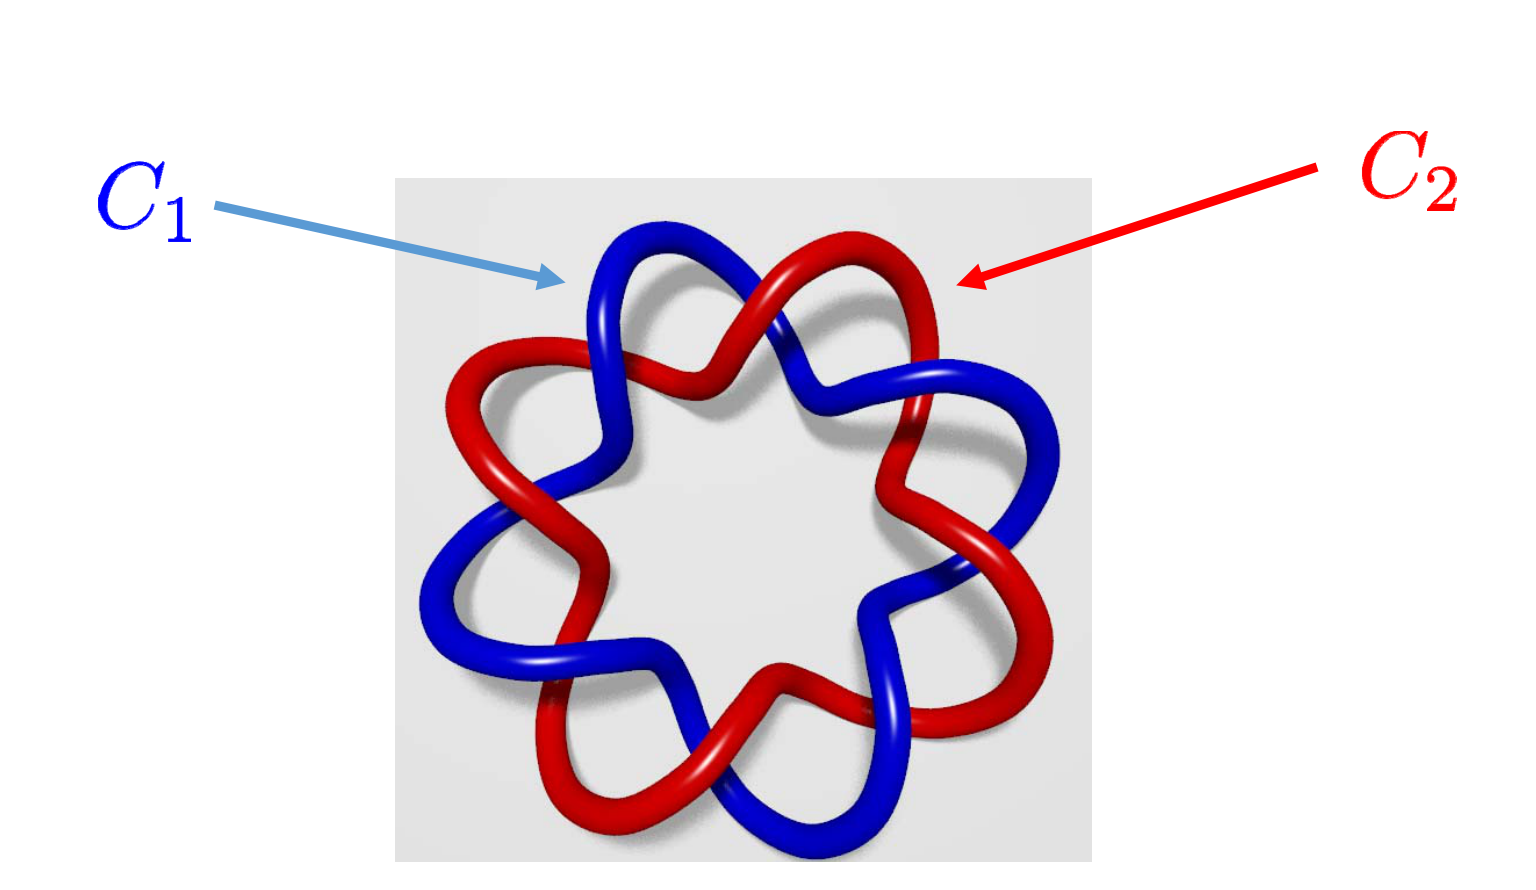
\includegraphics[width=0.55\textwidth]{figures/fig05.png}
  \caption{$\mathbb{R}^3$ 中两条相互链接的曲线 $C_1$ 与 $C_2$。（原文 Fig.~5，第 62 页）}
  \label{fig:5}
\end{figure}

\medskip
\noindent\textbf{评注}：$L(C_1,C_2)$ 的积分公式由 Gauss 于 1833 年发现。它与两个电流圈互感系数的 Neumann 公式有某些相似之处，但实际上相当不同。

我们断言 $L(C,C')$ 实际上是一个整数，它度量 $C$ 与 $C'$ 的链接。在静磁学中，如果我们不担心反转定向的时空变换，可以把 $\vec B$ 看作定义了 $\mathbb{R}^3$ 上的一个 $1$-形式，即 $B=B^idx^i$。类似地，可以把电流 $\vec J$ 看作定义了一个 $2$-形式 $J=\frac{1}{2}\epsilon_{ijk}J^idx^jdx^k$。这里我们用的是 $\mathbb{R}^3$ 中 $1$-形式与 $2$-形式之间的 Hodge 对偶，以及由欧氏度规给出的向量与 $1$-形式的等同。

无论如何，把 $B$ 等同于 $1$-形式、$J$ 等同于 $2$-形式之后，Biot–Savart 定律等价于：

\begin{equation}
  dB=J
  \tag{2.262}
  \label{eq:2.262}
\end{equation}

而所做的功正是 $\int_{C'}B$。

现在取 $I=1$，并令 $D'$ 是张在 $C'$ 上的一个定向圆盘，如图 6 所示。然后我们计算流过 $D'$ 的总电流：

\begin{equation}
  \begin{aligned}
    \oint_{C'}B&=\int_{D'}dB=\int_{D'}J\\
    &=\int_{D'}d\xi^\alpha\wedge d\xi^\beta\,
    \frac{\partial x^m}{\partial\xi^\alpha}\frac{\partial x^n}{\partial\xi^\beta}
    \frac{1}{2}\epsilon_{mnj}\oint_C\frac{dx^j(t)}{dt}\delta^{(3)}\big(\vec x(\xi)-\vec x(t)\big)
  \end{aligned}
  \tag{2.263}
  \label{eq:2.263}
\end{equation}
% [Tutor Note: 从 (2.263) 到「每个横截交点贡献 $\pm1$」省掉了一步：把沿 $C$ 的 $\delta^{(3)}$ 积分与 $\int_{D'}$ 交换次序后，$\int_{D'}d\xi^1d\xi^2\,\delta^{(3)}(\vec x(\xi)-\vec x(t))$ 只在 $D'$ 与 $C$ 横截相交的那些 $\xi$ 处非零，其值为 $1/|n\cdot\dot x(t)|$（$n$ 为 $D'$ 的法向）；再乘上 $\frac{1}{2}\epsilon_{mnj}\frac{\partial x^m}{\partial\xi^\alpha}\frac{\partial x^n}{\partial\xi^\beta}\dot x^j$——即 $\dot x$ 与 $D'$ 两条切向量的混合积——恰好约成 $\pm1$，符号由 $D'$ 的定向（由 $C'$ 诱导）与 $C$ 的定向共同决定。]

\begin{figure}[htbp]
  \centering
  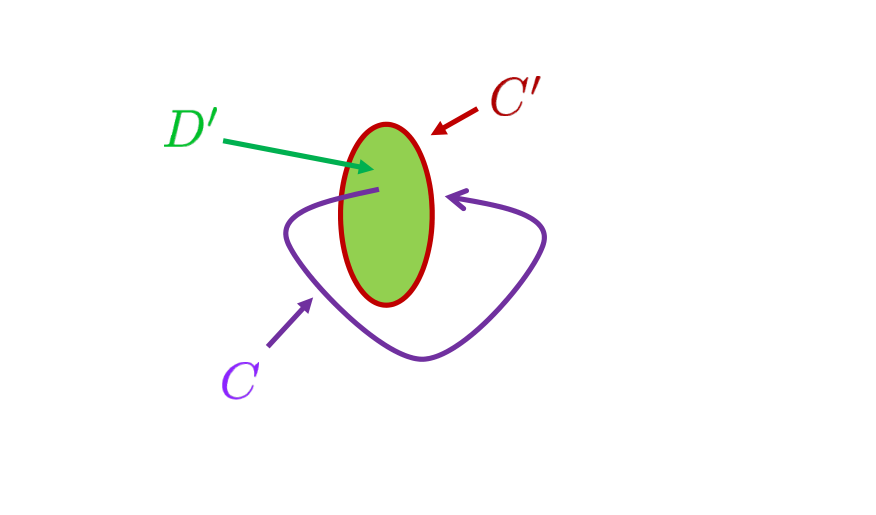
\includegraphics[width=0.42\textwidth]{figures/fig06.png}
  \caption{若用圆盘 $D'$ 填充 $C'$，则可证明 $L(C,C')$ 计数 $C'$ 与 $D'$ 的带符号相交数，因而是一个整数。（原文 Fig.~6，第 63 页）}
  \label{fig:6}
\end{figure}

其中 $\xi^\alpha$ 是 $D'$ 上的一些坐标。容易看出，在最后一个表达式中，$D'$ 与 $C$ 的每个横截\emph{相交}按定向贡献 $\pm1$：$C'$ 的定向在 $D'$ 上诱导出一个定向，而 $C$ 是定向的。这个带定向的相交数就是环绕数的定义之一。由这一解释，$L(C,C')$ 显然在 $D'$ 或 $C$ 或 $C'$ 的连续形变下不变，只要 $C$ 与 $C'$ 不交叉。

既然 $L(C,C')$ 是 $C$ 与 $C'$ 位置的\emph{连续}函数，另一方面它又是\emph{整数}，因此它是一个\emph{拓扑不变量}。注意，如果我们允许 $C$ 与 $C'$ 交叉，这个拓扑不变量就可能改变。当 $C$ 与 $C'$ 交叉时，公式 \eqref{eq:2.261} 变得不良定义，于是这个整数可以跳变。

\medskip
\noindent\textbf{练习}（\emph{拓扑不变性的显式验证}）\quad 证明 $I(C_1,C_2)$ 在 $\vec x_1(t)$ 的小形变下不变，做法是对公式 \eqref{eq:2.261} 作显式变分。

\medskip
\noindent\textbf{练习}\quad 定义 $\mathbb{R}^3-\{0\}$ 上的 $2$-形式

\begin{equation}
  \omega(x):=\frac{1}{8\pi}\frac{\epsilon_{ijk}x^idx^jdx^k}{|x|^3}
  \tag{2.264}
  \label{eq:2.264}
\end{equation}

a.) 证明：当限制到单位球面 $S^2\subset\mathbb{R}^3-\{0\}$ 上时，形式 $\omega$ 限制为体积等于 $1$ 的标准体积形式。

b.) 证明 Gauss 环绕数可以优雅地表示为：

\begin{equation}
  L(C_1,C_2)=\int_{C_1}\int_{C_2}\omega(x_1-x_2)
  \tag{2.265}
  \label{eq:2.265}
\end{equation}

\medskip
% [Tutor Note: 上一题 a.) 与 b.) 之间有一个容易漏掉的因子 2。(2.265) 里要展开 $\omega(x_1-x_2)$，必须用 $d(x_1-x_2)=dx_1-dx_2$ 并把 $dx_1\wedge dx_1=dx_2\wedge dx_2=0$ 用上：$d(x_1-x_2)^j\wedge d(x_1-x_2)^k=-2\,dx_1^j\wedge dx_2^k$，于是 $\omega(x_1-x_2)=-\frac{1}{4\pi}\epsilon_{ijk}(x_1-x_2)^idx_1^jdx_2^k$，与 (2.261) 的被积函数逐项相同（$1/8\pi$ 与 $2$ 一起给出 $1/4\pi$，负号则与 (2.261) 的 $-\frac{1}{4\pi}$ 一致）。若直接把 $d(x_1-x_2)$ 当成 $dx_1$，就会漏掉这个因子 2，并误以为 (2.257)、(2.265) 与 (2.261) 相差一个因子 $-2$。另外这一题里 $I(C_1,C_2)$ 按上下文应为 $L(C_1,C_2)$，原文如此，译文照录。]

% =====================================================================
%  c08：原印刷页 64–71（PDF p.65–72）
%  §2.2.16、§2.2.17、§2.2.18（三者均为 2.2.x 三级标题，故用 \subsubsection；
%  父 \section 与 \subsection 在 c03 片段中定义，本片段不补）
%  片段开头是原书图 7、图 8 的图注页（这两张图的正文讨论在 c07 片段末尾），
%  故本片段第一行即插图；公式编号 (2.266)–(2.298) 连续无缺。
% =====================================================================

\begin{figure}[htbp]
  \centering
  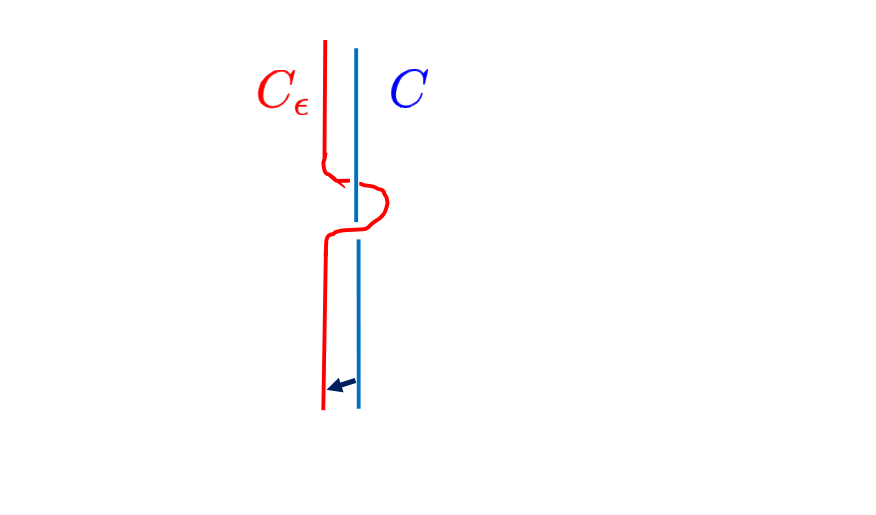
\includegraphics[width=0.45\textwidth]{figures/fig07.png}
  \caption{把 $C$ 沿法向作无穷小位移到 $C_\epsilon$，可能导致非平凡的自环绕，因为法向量可能绕着转。正因如此，$L(C,C)$ 是不良定义的。（原文 Fig.~7，第 64 页）}
  \label{fig:7}
\end{figure}

% 注意：figures/fig08.png 的裁切范围偏上，把图 7 的图形与其图注一并裁了进来（图 8 的图形在下方）。
% 此处按 brief 指定路径插入，未改动 figures/ 目录；若需出版质量，请重裁 fig08.png 后再编译。

\begin{figure}[htbp]
  \centering
  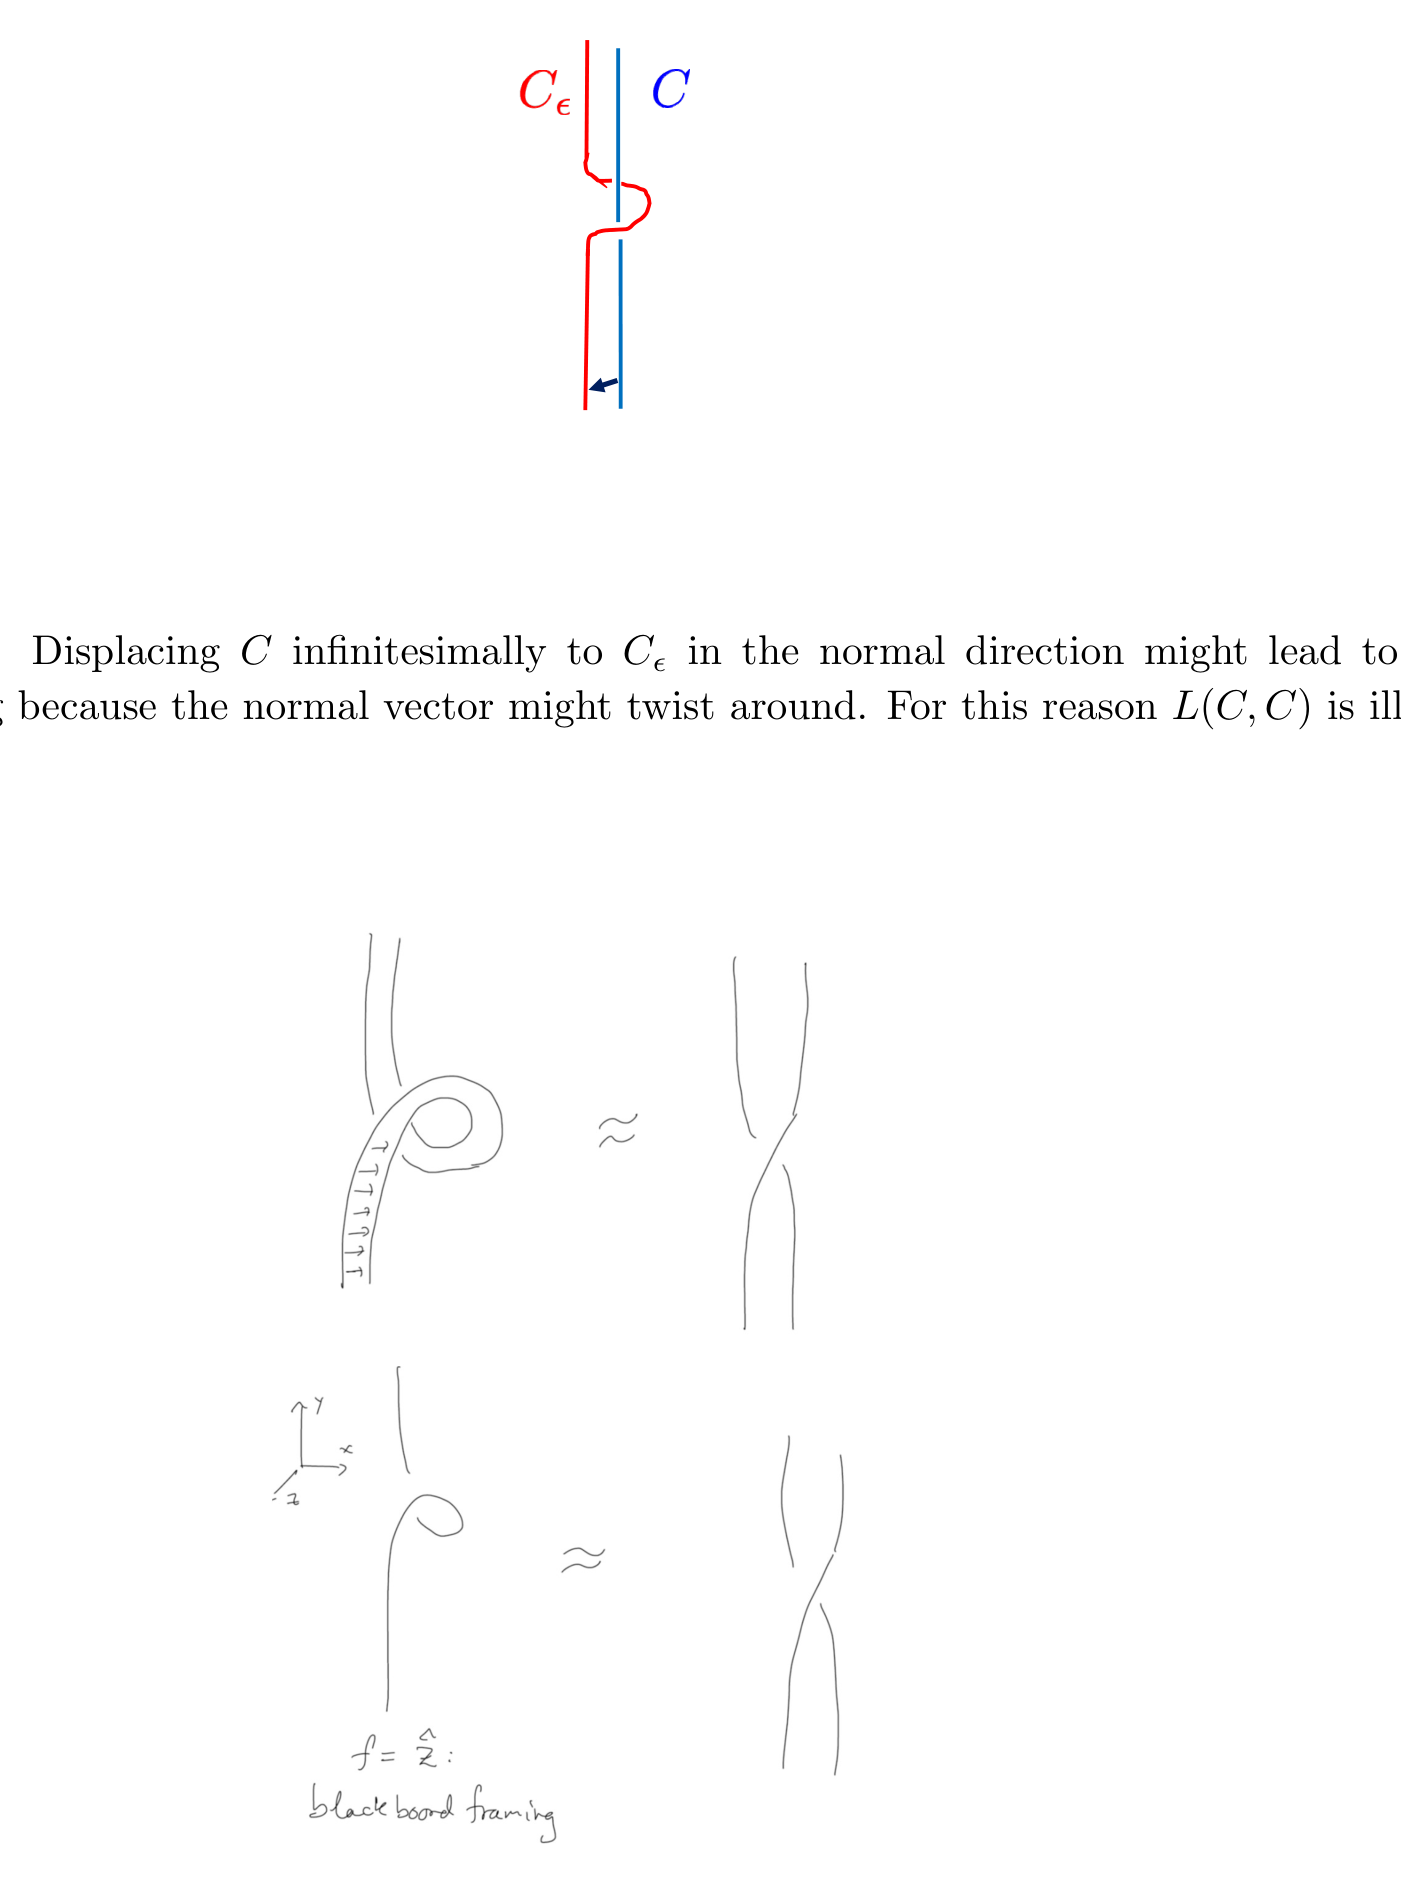
\includegraphics[width=0.55\textwidth]{figures/fig08.png}
  \caption{图示标架效应的不同但等价的画法。注意左下角：不加标架时，可以把绳子拉紧成一条直线。量子线缺陷依赖标架这一事实，会导致对第一 Reidemeister 移动的量子修正，如下文所述。（原文 Fig.~8，第 64 页）}
  \label{fig:8}
\end{figure}

\subsubsection{标架反常与缎带} % 原文: 2.2.16 The Framing Anomaly And Ribbons

以上所有讨论对 $\alpha\ne\beta$ 的那些项都运作良好。然而 $\alpha=\beta$ 时的环绕数还需要进一步讨论。正如自感（self-inductance）比互感（mutual inductance）要微妙得多，自环绕数也远比互环绕数微妙。自环绕数的公式显然在 Green 函数的重合点处有奇点。

这完全讲得通，正如图~\ref{fig:7} 所说明的。要定义 $L(C,C)$，必须把 $C$ 沿法向作无穷小位移，然后计算 $C$ 与其位移版本的互环绕数。但这显然是不良定义的，因为 $C$ 可能绕着自己转好几圈。在 Chern-Simons 理论中，这被称为\emph{标架反常}（framing anomaly）。

\textbf{定义}：\emph{Wilson 线算符的标架}（framing），是指 $\gamma\subset M_3$ 的法丛的一个处处非零截面，模去同伦（连续形变）。若 $s:\gamma\to N(\gamma)$ 是法丛的一个处处非零截面，我们就把标架记为 $f=[s]$。

更口语地说：我们可以说，在量子理论中 Wilson 线算符是与\emph{缎带}（ribbon）相联系的。当我们试图写出链环不变量时，这一点会有重要含义。预告见图~\ref{fig:8}。

\textbf{评注}

\begin{enumerate}
  \item 给定一个非零截面 $s:\gamma\to N(\gamma)$，我们可以把它拧上 $n$ 圈，$n$ 为任意整数。这里我们用到定向：Wilson 线是对一条定向曲线 $\gamma$ 定义的，因此垂直于线的圆盘上有确定的定向。于是拧 $n$ 圈就是在圆盘内作 $2\pi n$ 的逆时针旋转。注意这些标架并不构成 Abel 群：你不能把 $f_1+f_2$ 相加。因为若试图把法丛的两个截面相加，无法保证其和仍然非零。尽管如此，把一个整数加到一个标架上是有意义的：$f\to f+n$、$n\in\mathbb{Z}$；而且任意两个标架都可以通过这样的整数平移互相联系。数学上我们说，标架构成一个 $\mathbb{Z}$-torsor（$\mathbb{Z}$-主齐性空间）。\footnote{一般地，对任意群 $G$，若 $G$ 在集合 $S$ 上的作用既自由又传递，则称 $S$ 是一个 $G$-torsor。可以把 $S$ 想成 $G$ 的一份拷贝，只是没有选定单位元。主 $G$-丛的纤维就是 $G$-torsor 的好例子。}
  % [Tutor Note: 术语取舍。$G$-torsor 的中译常见「$G$-主齐性空间」与「$G$-扭子」两种，此处取前者，因为脚注 24 把它说成「未选单位元的 $G$ 的拷贝」，与主丛纤维的语义最贴；「扭子」又易与 twistor（扭量）相混。另注意作者特意强调标架不构成 Abel 群（不能相加 $f_1+f_2$），只能作 $\mathbb{Z}$-平移，这正是 torsor 与群的区别所在，写公式时务必用 $f+n$ 而不是 $f_1+f_2$。]

  \item 我们所发现的是：在 $W(r,\gamma)$ 的量子定义中，为了定义线缺陷，我们需要额外附加一份数据，即曲线 $\gamma$ 的标架。因此我们把记号改为
  \begin{equation}
    W(n,\gamma)\to W(n,\gamma,f)
    \tag{2.266}
    \label{eq:2.266}
  \end{equation}
  注意给定 $\gamma$ 与 $f$，存在良定义的同痕类 $\gamma+f$，而我们可以用
  \begin{equation}
    L_f(\gamma):=L(\gamma,\gamma+f)
    \tag{2.267}
    \label{eq:2.267}
  \end{equation}
  来定义自环绕数。因此，(2.255) 的一个更准确的版本是
  \begin{equation}
    \Big\langle\prod_{\alpha}W(r_{\alpha},\gamma_{\alpha},f_{\alpha})\Big\rangle
    =\mathcal{N}\cdot\exp\left[\sum_{\alpha<\beta}\frac{2\pi\mathrm{i}}{2\kappa}r_{\alpha}r_{\beta}L(\gamma_{\alpha},\gamma_{\beta})
    +\sum_{\alpha}\frac{2\pi\mathrm{i}}{4\kappa}r_{\alpha}^{2}L_{f_{\alpha}}(\gamma_{\alpha})\right]
    \tag{2.268}
    \label{eq:2.268}
  \end{equation}
  % [Tutor Note: (2.268) 的两个求和不能合并：$\sum_{\alpha<\beta}$ 只计互环绕，自环绕 $L_{f_\alpha}(\gamma_\alpha)$ 单列，且系数是 $\frac{2\pi\mathrm{i}}{4\kappa}$（比互环绕项的 $\frac{2\pi\mathrm{i}}{2\kappa}$ 多一个 $1/2$）。若把 $\sum_{\alpha<\beta}$ 写成 $\sum_{\alpha,\beta}$ 或 $\sum_{\alpha\le\beta}$，就会重复计数互环绕，并把自环绕项误算成互环绕项。自查办法：令所有 $\gamma_\alpha$ 互不链接、只各自带标架、且 $r_\alpha=n$，则 (2.268) 必须退化为纯相位 $\exp\big[\sum_\alpha\frac{2\pi\mathrm{i}}{4\kappa}n^{2}L_{f_\alpha}\big]$，与 (2.270) 在 $N=1$ 时一致。]

  \item 注意
  {\small\itshape ［原文标记：\ensuremath{\clubsuit} 会不会是 $-n$？需要核对。\ensuremath{\clubsuit}］}
  % [原文待办标记，原文 p.65 页边，作者对标架平移方向的正负号存疑]
  \begin{equation}
    L_{f+n}(\gamma)=L_f(\gamma)+n
    \tag{2.269}
    \label{eq:2.269}
  \end{equation}
  % [Tutor Note: 符号约定易错。(2.269) 里 $+n$ 对应「在法向圆盘内逆时针旋转 $2\pi n$」，作者自己在页边写「Could it be $-n$?」，说明他也没定下来。可靠的定号办法是从 (2.270) 反推：把 (2.269) 代入 (2.268) 的自环绕项，$f\to f+N$ 给出的比值必须是 $e^{2\pi\mathrm{i}Nn^{2}/(4\kappa)}$；若 (2.269) 取 $-n$，则该相位变号，「自旋为 $n^{2}/4\kappa$」这一物理解释随之翻转，与 (2.270) 不符。]

  因此
  \begin{equation}
    W(n,\gamma,f+N)=\left(e^{2\pi\mathrm{i}\frac{n^{2}}{4\kappa}}\right)^{N}W(n,\gamma,f)
    \tag{2.270}
    \label{eq:2.270}
  \end{equation}
  我们说 $e^{2\pi\mathrm{i}\frac{n^{2}}{4\kappa}}$ 是线缺陷的\emph{自旋}（spin）。（有些作者会说 $\frac{n^{2}}{4\kappa}\bmod\mathbb{Z}$ 是线缺陷的自旋。例如文献 [28] 就是在这个意义上使用的。当我们讨论与 RCFT 的关系时，这将与相应共形场的自旋、以及手征代数表示的量子维度联系起来。）

  \item 若 $\gamma\subset\Sigma_2$ 落在一个形如 $\Sigma_2\times\mathbb{R}$ 的 3-流形中，则我们可以把线缺陷 $W(n,\gamma,f)$ 视为 Hilbert 空间上的算符。若选取指向未来时间的自然标架，则该算符可以等同于我们在 Heisenberg 的故事里讨论过的算符 $\widehat{W}(n\gamma)$。

  \item \underline{线缺陷标号的等同}：注意 $n\to n+2\kappa$ 使关联函数不变。这与量子等同
  \begin{equation}
    W(n+2\kappa,\gamma,f)\cong W(n,\gamma,f)
    \tag{2.271}
    \label{eq:2.271}
  \end{equation}
  一致，后者是我们在考虑 Hilbert 空间 $\mathcal{H}(\Sigma_2)$ 上的算符时得到的。虽然相似，(2.271) 在概念上是不同的，因为它涉及的是插入路径积分中的线缺陷，而不是曲面物理 Hilbert 空间上的算符。

  从公式 (2.259) 我们看到，也可以通过给规范场施加边界条件来给出 Wilson 线可观测量的定义，而不是对光滑规范场作积分并添加源项（这是我们迄今一直做的）。从这个观点看，支撑在 $\gamma$ 上的线缺陷是这样定义的：挖掉 $\gamma$ 周围半径为 $\epsilon$ 的小管状邻域；而要定义荷为 $n$ 的缺陷，我们要求规范场满足这样的边界条件——若 $C(\epsilon)$ 是这个管状邻域边界上的小环绕曲线，则插入 $W(n,\gamma,f)$ 的路径积分具有边界条件
  \begin{equation}
    \lim_{\epsilon\to0}e^{\mathrm{i}\oint_{C(\epsilon)}A}=e^{-2\pi\mathrm{i}n/(2\kappa)}
    \tag{2.272}
    \label{eq:2.272}
  \end{equation}
  注意从这个观点看，我们自动得到等同 $n\sim n+2\kappa$。\footnote{这个论证有一个不严谨的版本如下：我们作一个奇异的规范变换，其变换函数在 Wilson 线附近形如 $g\sim e^{\mathrm{i}\phi}$，其中 $\phi$ 是方位角。Chern-Simons 作用量的改变量写作
  \begin{equation}
    \frac{\kappa}{2\pi}\int d(Ad\phi)+2\cdot\frac{\kappa}{2\pi}\int A\,d^{2}\phi
    \tag{2.273}
    \label{eq:2.273}
  \end{equation}
  这里我们说 $d(d\phi)=2\pi\delta^{(2)}(x)$，其中 $\delta^{(2)}(x)$ 是支撑在 Wilson 线上的 Dirac 测度。这个略显可疑的方程中的常数，是通过在一个圆盘上积分并施加 Stokes 定理得到的。在目前这个做法里没有边界，所以我们可以丢掉第一项。净效应是把 $n$ 平移为 $n+2\kappa$。}
  % [Tutor Note: (2.272) 的相位是 $e^{-2\pi\mathrm{i}n/(2\kappa)}$，而和乐 $e^{\mathrm{i}\oint A}$ 的周期是 $2\pi$，所以 $n$ 的模长是 $2\kappa$（与 (2.271) 的 $n\to n+2\kappa$、以及本节处处出现的荷格 $\mathbb{Z}/2\kappa\mathbb{Z}$ 一致），不是 $\kappa$。若把指数误写成 $e^{-2\pi\mathrm{i}n/\kappa}$，就会得到荷格 $\mathbb{Z}/\kappa\mathbb{Z}$，与 (2.271) 直接冲突。另外脚注 25 中 $2\cdot\frac{\kappa}{2\pi}\int A\,d^{2}\phi$ 的因子 2 来自 $d(A\,d\phi)=dA\,d\phi-A\,d^{2}\phi$ 的展开（$\phi$ 是角函数，$d^{2}\phi$ 是奇异的），核对时不要把它当成手误。]

  \item \underline{线缺陷的「算符乘积」}。一般地，当我们有「平行」缺陷时，我们想定义缺陷的「算符乘积」概念。在目前情形下，我们可以用 (2.268) 来定义 Wilson 线缺陷的算符乘积。为了定义我们所谓的「平行曲线」，我们假定 $\gamma_2$ 可由 $\gamma_1$ 经一次无穷小标架位移得到，从而 $\gamma_2$ 同痕于 $\gamma_1+f_{12}$。我们同样可以说 $\gamma_2=\gamma_1+f_{21}$。注意
  \begin{equation}
    L_{f_{12}}(\gamma_1)=L_{f_{21}}(\gamma_2)=L(\gamma_1,\gamma_2)
    \tag{2.274}
    \label{eq:2.274}
  \end{equation}
  现在考虑线缺陷的乘积：
  \begin{equation}
    W(n_1,\gamma_1,f_1)W(n_2,\gamma_2,f_2)
    \tag{2.275}
    \label{eq:2.275}
  \end{equation}
  假定所有其它线缺陷与 $\gamma_1$、$\gamma_2$ 的链接方式都相同，即
  \begin{equation}
    L(\gamma_1,\gamma_{\beta})=L(\gamma_2,\gamma_{\beta})\qquad\beta>2
    \tag{2.276}
    \label{eq:2.276}
  \end{equation}
  若 $\gamma_2$ 是由 $\gamma_1$ 经无穷小位移得到的，这一点自动成立。在条件 (2.276) 之下，我们可以把线缺陷的乘积 (2.275) 替换为单个线缺陷。为此我们写
  \begin{equation}
    \begin{aligned}
      f_1 &= f_{12}+N_{12}\\
      f_2 &= f_{21}+N_{21}
    \end{aligned}
    \tag{2.277}
    \label{eq:2.277}
  \end{equation}
  其中 $N_{12},N_{21}\in\mathbb{Z}$。于是有
  \begin{align}
    W(n_1,\gamma_1,f_1)W(n_2,\gamma_2,f_2)
      &\cong e^{2\pi\mathrm{i}\left(\frac{n_1^{2}}{4\kappa}N_{12}+\frac{n_2^{2}}{4\kappa}N_{21}\right)}W(n_1+n_2,\gamma_1,f_{12}) \notag\\
      &\cong e^{2\pi\mathrm{i}\left(\frac{n_1^{2}}{4\kappa}N_{12}+\frac{n_2^{2}}{4\kappa}N_{21}\right)}W(n_1+n_2,\gamma_2,f_{21})
    \tag{2.278}
    \label{eq:2.278}
  \end{align}

  \item \underline{单极子算符}。三维规范理论中一类重要的局域算符是单极子算符（monopole operator）。对具有规范群 $G$ 的一般规范理论，它们通过选取一个嵌入 $\mu:U(1)\to G$ 而得到。这允许把一个磁荷为 $\mu$ 的 Dirac 单极子嵌入 $G$ 规范理论，其中 $F^{\mathrm{Dirac}}=2\pi\frac{\sin\theta d\theta d\phi}{4\pi}$。然后我们可以在点 $p$ 处定义一个奇异的 $G$ 联络：用半径为 $\varepsilon$ 的小球包围 $p$，并要求当 $\varepsilon\to0$ 时
  \begin{equation}
    F\to\mu(F^{\mathrm{Dirac}})
    \tag{2.279}
    \label{eq:2.279}
  \end{equation}
  这个奇异的边界条件定义了一个荷为 $\mu$ 的点缺陷，即「单极子算符」$M_{\mu}(p)$。

  然而，若回想 Chern-Simons 作用量的规范变分 (2.45)，我们就会看到 $M_{\mu}(p)$ 不是规范不变的，而是按
  \begin{equation}
    M_{\mu}(p)\to e^{\mathrm{i}\kappa\mu(\epsilon(p))}M_{\mu}(p)
    \tag{2.280}
    \label{eq:2.280}
  \end{equation}
  变换。因此这个算符不是规范不变的。在一个非拓扑理论中，这个问题可以通过附加一条 Wilson 线、或乘上某个带相反荷的其它带电算符来补救；但在拓扑的 Chern-Simons 理论中，无法引入这些算符。

  {\small\itshape ［原文标记：\ensuremath{\clubsuit} 这里需要解释的东西还很多……\ensuremath{\clubsuit}］}
  % [原文待办标记，原文 p.67 页边]

  \item \underline{一形式对称性}。文献 [23] 中提出，量子场论里关于整体对称性的许多熟知事实，都能很好地推广为与更高维缺陷相联系的数学结构的变换。特别地，「一形式对称性」是与余维二维缺陷相联系的。当这些缺陷沿一条无穷小环绕与一维缺陷相链接时，结果是一个新的余维二维缺陷。这就是 [23] 的「一形式对称性」。在目前情形下，实现一形式对称性的对象本身就是那些一维缺陷，因而是 Wilson 线。它们构成一个同构于 $\mathbb{Z}/2\kappa\mathbb{Z}$ 的 Abel 群，这正是上述「算符乘积」下的群。由于上述简单的环绕规则，$W(n,\gamma)$ 在一形式对称群下的「荷为 $n$」。也就是说，它位于定义表示的第 $n$ 次幂之中。
  % 注：「第 $n$ 次幂」指 $W(n,\gamma)$ 同构于 $W(1,\gamma)$ 的 $n$ 重算符乘积；由 (2.271) 可知 $n$ 应读作 $\mathbb{Z}/2\kappa\mathbb{Z}$ 中的元素。

  \item {\small\itshape ［原文标记：COMMENT ON WHAT HAPPENS FOR WILSON LINES IN A GENERAL 3-MANIFOLD（评述一般 3-流形中 Wilson 线会发生什么）］}
  % [原文待办标记，原文 p.68：全大写，是作者留给自己的写作待办，正文内容尚未写出]
\end{enumerate}

\subsubsection{一个拓扑反常：归一化因子 $\mathcal{N}$} % 原文: 2.2.17 A Topological Anomaly: The Normalization Factor: N

如我们所说，归一化因子在形式上与度规无关，因为迄今为止我们并不需要使用度规。然而，要定义路径积分，我们必须对规范对称性作规范固定（gauge-fix），而任何规范固定的选择都会破坏路径积分形式上的拓扑对称性。所幸，拓扑不变性被破坏的方式是可计算的，而且这种破坏有很好的物理意义。

最标准的规范固定方式，是在 $M_3$ 上引入一个 Riemann 度规，并（在 Abel 情形）选取规范切片：
\begin{equation}
  d*A=\operatorname{vol}(g)g^{\mu\nu}D_{\mu}A_{\nu}=0
  \tag{2.281}
  \label{eq:2.281}
\end{equation}
这会把所有规范自由度固定到调和形式 $A\to A+\omega$ 为止。因此会剩下一个有限维环面 $\mathcal{H}^{0}(M_3;U(1))$ 的未固定规范变换。

标准的规范固定方式是在 BRST 步骤中引入 Faddeev-Popov 鬼场：我们引入反对易的零形式（取规范群的伴随表示）$c,b$，其鬼数分别为 $+1$、$-1$，并引入微分
\begin{equation}
  \begin{aligned}
    Q(A) &= Dc\\
    Q(c) &= 0\\
    Q(b) &= H\\
    Q(H) &= 0
  \end{aligned}
  \tag{2.282}
  \label{eq:2.282}
\end{equation}
并且我们往作用量里添加
\begin{equation}
  Q\Big(\mathrm{i}\int b\,d*A\Big)=\mathrm{i}\int b\,d*dc+\mathrm{i}\int H\,d*A
  \tag{2.283}
  \label{eq:2.283}
\end{equation}
我们应把 $H$ 看作 Lagrange 乘子。\footnote{通常在 BRST 步骤中会给 $H$ 加一个高斯项。但在目前情形下，那会破坏作用量的一阶（first-derivative）性质，并使这个漂亮的故事复杂化。} 对 $b,c$ 的积分给出
\begin{equation}
  \det' *d*d
  \tag{2.284}
  \label{eq:2.284}
\end{equation}
% [Tutor Note: 逻辑跳步。(2.283) 中没有通常的高斯项 $H^{2}$（脚注 26 说明：那会破坏作用量的一阶性质），所以 $H$ 是 Lagrange 乘子，对 $H$ 积分给出 $\delta(d*A)$ 而非高斯权重——这正是 (2.288) 里 Jacobian 的来源。另外 (2.284) 的 $\det'$ 来自对反对易场 $b,c$（鬼数 $+1,-1$，两者独立而非互为共轭）作 Grassmann 积分，结果是一个完整的行列式而不是平方根，带撇表示去掉零模；把它与 (2.289) 分母上的 $\det^{1/2}$ 对比时，务必分清哪个是 0-形式上的、哪个是 1-形式上的。作者在页边写「Should discuss zeromode」，正是指这个撇号尚未交代清楚。]

其中 $*d*d$ 是 0-形式上的标准度规 Laplacian。
{\small\itshape ［原文标记：\ensuremath{\clubsuit} 应讨论零模 \ensuremath{\clubsuit}］}
% [原文待办标记，原文 p.69 页边]

与此同时，我们可以把 Lagrange 乘子场重新标度为 $H=\text{const.}*\phi$，其中 $\phi\in\Omega^{3}(M_3)$，从而得到作用量
\begin{equation}
  \exp\Big[\frac{\mathrm{i}k}{2\pi}\int_{M_3}\big(AdA+\phi*d*A\big)
  =\exp\Big[\frac{\mathrm{i}k}{2\pi}\int_{M_3}\Phi*D\Phi\Big]
  \tag{2.285}
  \label{eq:2.285}
\end{equation}
% [Tutor Note: (2.285) 的括号在原文里就不配对（左端作 $\exp\big[\cdots\big($、右端作 $\big(\cdots\big]$），此处照原文转写；由右端形式可知左端应为 $\exp\big[\frac{\mathrm{i}k}{2\pi}\int_{M_3}(AdA+\phi*d*A)\big]$，这是原文的排版笔误。又：本小节 (2.285)–(2.290) 用的是斜体 $k$，而 (2.268) 等处用的是 $\kappa$，二者是同一个量（CS 能级／耦合常数），作者在此换了字母；不要把它当成第二个独立的耦合常数，否则 (2.289) 的 $2\pi\mathrm{i}k*d$ 与 (2.283) 的 $\frac{\kappa}{2\pi}$ 就无法配平。还有一处笔误：$\Phi*D\Phi$ 中的 $D$ 应即下面 (2.286) 的 $D_{+}$。]

其中
\begin{equation}
  \Phi=\begin{pmatrix}A\\ \phi\end{pmatrix}
  \qquad\qquad
  D_{+}=\begin{pmatrix}*d & 0 & 0\\ 0 & 0 & d*\\ 0 & d* & 0\end{pmatrix}
  \tag{2.286}
  \label{eq:2.286}
\end{equation}
这里
\begin{equation}
  D_{+}:\Omega^{\mathrm{odd}}(M_3)\to\Omega^{\mathrm{even}}(M_3)
  \tag{2.287}
  \label{eq:2.287}
\end{equation}
是 $D_{+}=*d+d*$。这可以解释为一个扭化 Dirac 算符（twisted Dirac operator）。当我们用非 Abel 理论重新审视这个计算时，会回到这一点。

后文在 ［原文标记：****］ 节中，我们会把 $D_{+}$ 看作扭化 Dirac 算符，并利用关于奇数维流形上 Dirac 算符行列式的一些一般事实。% [原文待办标记，原文 p.69：作者用「****」作节号占位，始终未填]
眼下我们改用一些 Hodge 理论。相关事实的综述见 F 节。算符 $*d:\Omega^{1}\to\Omega^{1}$ 是自伴的，\footnote{$(*d)^{\dagger}=d^{\dagger}*^{\dagger}=\pm*d**=\pm*d$。{\small\itshape ［原文标记：SIGN????（符号存疑）］}}% [原文待办标记，原文 p.69 脚注 27，作者对自己的符号推导存疑]
并且可以在 $\operatorname{Im}d^{\dagger}\subset\Omega^{1}$ 上对角化，谱为 $\mu_{n}^{(1)}$。这是一个类 Dirac 算符，其谱上下无界。与此同时，$\operatorname{Im}d\subset\Omega^{1}$ 上 $dd^{\dagger}$ 的谱为 $(\lambda_{n}^{(0)})^{2}$。

对 $H$ 的积分给出一个 delta 函数，于是我们得到一个 Jacobian
\begin{equation}
  \int_{\Omega^{1}}[dA]\,\delta(d*A)[\ldots]
  =\int_{\operatorname{Im}d^{\dagger}}[dA]\,\frac{1}{\prod_{n}|\lambda_{n}^{(0)}|}[\ldots]
  \tag{2.288}
  \label{eq:2.288}
\end{equation}
然后作剩下的积分给出行列式：
\begin{equation}
  \frac{\det' *d*d}{\det^{1/2}\Big(\frac{1}{2e^{2}}d^{\dagger}d+2\pi\mathrm{i}k*d\Big)\Big|_{\operatorname{Im}d^{\dagger}}}\;
  \frac{1}{\prod_{n}|\lambda_{n}^{(0)}|}
  \tag{2.289}
  \label{eq:2.289}
\end{equation}
第一个因子可以给出一个相位。我们用 $\zeta$-函数作正规化，于是
\begin{equation}
  \zeta(s)=\sum_{n}\Big(\frac{1}{2e^{2}}\big(\mu_{n}^{(1)}\big)^{2}+2\pi\mathrm{i}k\mu_{n}^{(1)}\Big)^{-s}
  \tag{2.290}
  \label{eq:2.290}
\end{equation}
注意存在谱不对称性。在 $e^{2}\to\infty$ 的极限下我们得到
\begin{equation}
  \operatorname{Im}\big(-\zeta'(0)\big)=\frac{\pi}{2}\eta(*d+d*)
  \tag{2.291}
  \label{eq:2.291}
\end{equation}
这给出了 CS 理论标架反常的一个漂亮的推导。

$\eta$ 不变量\emph{确实}有度规依赖，但这种度规依赖是局域的。我们会在 3.2.1 节用非 Abel 情形重新讨论这一点时再谈它。其绝对值为
\begin{equation}
  \prod_{n}\frac{|\lambda_{n}^{(0)}|}{\sqrt{|\mu_{n}^{(1)}|}}=\exp\Big[-\frac{1}{4}\tau(M_3)\Big]
  \tag{2.292}
  \label{eq:2.292}
\end{equation}
其中 $\tau(M_3)$ 是 Ray-Singer 挠率（Ray-Singer torsion），或称解析挠率。它是一个拓扑不变量，如附录 F 所示。
% [Tutor Note: (2.288) 的等号用到了 Hodge 分解 $\Omega^{1}=\operatorname{Im}d\oplus\operatorname{Im}d^{\dagger}\oplus\mathcal{H}^{1}$，以及 $d*A$ 在 $\operatorname{Im}d$ 上的 Jacobian 恰为 $\prod_{n}|\lambda_{n}^{(0)}|$；作者未写出这一步。再注意 (2.291) 的 $\eta$ 项（相位）与 (2.292) 的 $\tau$ 项（模长）是同一个行列式的两部分：$\tau$ 的定义本身就含 $\zeta'(0)$（除 $\eta$ 项外的对称部分），所以把两者相乘时不可重复计入 $e^{-\tau/4}$，也不可把 (2.291) 的 $\pi/2$ 与 (2.292) 的 $1/4$ 混用。]

\begin{figure}[htbp]
  \centering
  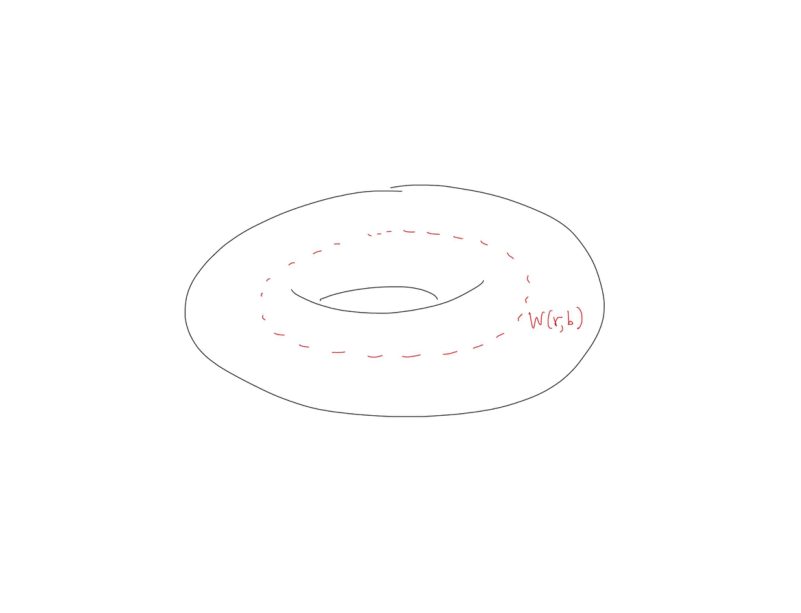
\includegraphics[width=0.55\textwidth]{figures/fig09.png}
  \caption{把手体上的路径积分（本图中是一个实心环面）定义了场之边界值的波泛函。在 Chern-Simons 理论的情形，它定义了围成该把手体的曲面的共形块空间中的一个特定状态。我们可以通过插入 Wilson 线缺陷这类非局域算符来改变该状态。（原文 Fig.~9，第 70 页）}
  \label{fig:9}
\end{figure}

\subsubsection{统一路径积分与 Hamilton 观点：由 Wilson 线生成的状态} % 原文: 2.2.18 Uniting The Path Integral And Hamiltonian Viewpoints: States Created By Wilson Lines

相当一般地，假设我们有一个 $d$ 维时空中的场论，场 $\phi$ 取值于某个靶空间 $\mathcal{T}$。若该理论由路径积分定义，那么当 $X$ 是一个 $d$ 维时空、其边界为 $\partial X=M$ 时，$X$ 上的路径积分就定义了与 $(d-1)$ 维流形 $M$ 相联系的 Hilbert 空间 $\mathcal{H}(M)$ 中的一个确定状态：
\begin{equation}
  \partial X=M\qquad\Rightarrow\qquad\psi_{X}\in\mathcal{H}(M).
  \tag{2.293}
  \label{eq:2.293}
\end{equation}
我们这里的记号是高度示意性的。例如，若我们在流形 $X$ 内部插入局域算符或其它缺陷，那就会改变我们所谓的 $X$ 是什么；而一般说来，这类插入肯定会使该状态改变。

方程 (2.293) 不难理解：为了定义路径积分，我们需要指定某些边界值 $\phi_\partial$，以便有合适的稳相近似和合适的经典变分问题。（$\phi_\partial$ 可能比场 $\phi$ 在 $\partial X$ 上的简单限制更为微妙。）我们可以把 $\mathcal{H}(M)$ 认定为边界条件空间上（适当可归一化的）波函数的空间，而具有特定边界条件 $\phi_\partial$ 的路径积分之值，被规定为状态 $\psi_X$ 在 $\phi_\partial$ 处的波函数值：
\begin{equation}
  \psi_X(\phi_\partial):=\mathit{PATH\ INTEGRAL\ WITH}\ \mathrm{b.c.}=\phi_\partial
  \qquad\Rightarrow\qquad
  \psi_X\in\mathcal{H}((M)
  \tag{2.294}
  \label{eq:2.294}
\end{equation}
% [Tutor Note: 原文 (2.294) 右端印作 $\mathcal{H}((M)$（多一个左括号、缺一个右括号），显系排版笔误，应为 $\mathcal{H}(M)$（与 (2.293) 一致）；此处照原文转写，以便与页面图像逐字对照。]

在基于「从几何范畴到张量范畴的函子」的场论公理化方法中，上述评述就变成了一条公理。（更确切地说，它是某些更基本公理的直接推论。）

把这一想法落实到目前 $U(1)$ Chern-Simons 理论的情形，做法如下。假设我们的 3-流形有一张边界曲面 $\Sigma_2$。先假定它是连通的。那么 3-流形 $M_3$ 就是所谓的把手体（handlebody）。注意存在群同态
\begin{equation}
  \iota:\pi_1(\Sigma_2,x_0)\hookrightarrow\pi_1(M_3,x_0)
  \tag{2.295}
  \label{eq:2.295}
\end{equation}
它诱导出同态
\begin{equation}
  \iota:H_1(\Sigma_2)\hookrightarrow H_1(M_3)
  \tag{2.296}
  \label{eq:2.296}
\end{equation}
这两个同态都会有很大的核：在图~3 中，如果我们按自然方式把曲面填满，那么所有 $a$-圈都映到零，而 $b$-圈保持非平凡。既然所有 $a$-圈都映到零，我们预期在算符方法里 $W(\gamma)\psi_{M_3}=\psi_{M_3}$ 对所有 $\gamma\in L_1$ 成立。这确实在 Stone-von Neumann 表示中挑出一条一维直线，从而挑出一个纯态。用该直线上某个非零向量 $\Psi_{M_3}$ 来表示这个态。

有意思的是，按上文建议的方式，通过插入一条荷为 $n_0\in\mathbb{Z}/2\kappa\mathbb{Z}$ 的 Wilson 线来改变 $X$，如图~\ref{fig:9} 所示。
{\small\itshape ［原文标记：\ensuremath{\clubsuit} 需要修图，使插入荷为 $n_0$ \ensuremath{\clubsuit}］}
% [原文待办标记，原文 p.71 页边]
一般地，我们可以考虑 $W(n_0\gamma)$，其中 $\gamma\in H_1(M_3;\mathbb{Z})$。这会产生一个新状态，它可以用非零向量 $\Psi_{M_3,n_0\gamma}$ 表示。设 $\hat\gamma\in H_1(\Sigma_2)$ 落在 $\iota$ 的原像中。显然
\begin{equation}
  \Psi_{M_3,n_0\gamma}=\widehat{W}(n_0\gamma)\Psi_{M_3}
  \tag{2.297}
  \label{eq:2.297}
\end{equation}
因为若把 Wilson 线施加到曲面上，我们可以让它「沉入」以获得图~\ref{fig:9} 中的图像。当然，这就是由下述条件确定的纯态（$\mathcal{H}(\Sigma_2)$ 中的一维直线）：它是 $W(\gamma')$ 的本征线，本征值为 $e^{2\pi\mathrm{i}\frac{\langle\gamma',n_0\gamma\rangle}{2\kappa}}$，对所有 $\gamma'\in L_b$ 成立。
\begin{equation}
  \widehat{W}(\gamma')\Psi_{M_3,n_0\gamma}
  =e^{2\pi\mathrm{i}\frac{\langle\gamma',n_0\gamma\rangle}{2\kappa}}\Psi_{M_3,n_0\gamma}
  \tag{2.298}
  \label{eq:2.298}
\end{equation}
事实上，(2.298) 也可以相当直接地推出：让 $\gamma'$ 同样「沉入把手体」，直到它与 $\gamma$ 相链接。

\begin{quote}
\small\itshape
［原文标记：***********************************************************

（1）讨论环面这一具体例子中的边界条件 $\phi_\partial$。

（2）现在推广到多个连通分支。它们的定向可以与 3-流形 $M_3$ 的定向一致或不一致，于是我们得到空间与对偶空间，即入射与出射空间。路径积分作为从入射到出射的线性变换。］
\end{quote}
% [原文待办标记，原文 p.71 页末：星号分隔的两条全大写写作提纲，作者尚未写成正文]

{\small\itshape ［原文标记：\ensuremath{\clubsuit} 需要修图：图中的表示应当画成缎带，且其标号是 $n_1$、$n_2$ 而不是 $\mu$、$\nu$ \ensuremath{\clubsuit}］}
% [原文待办标记，原文 p.71 页边]

\begin{figure}[htbp]
  \centering
  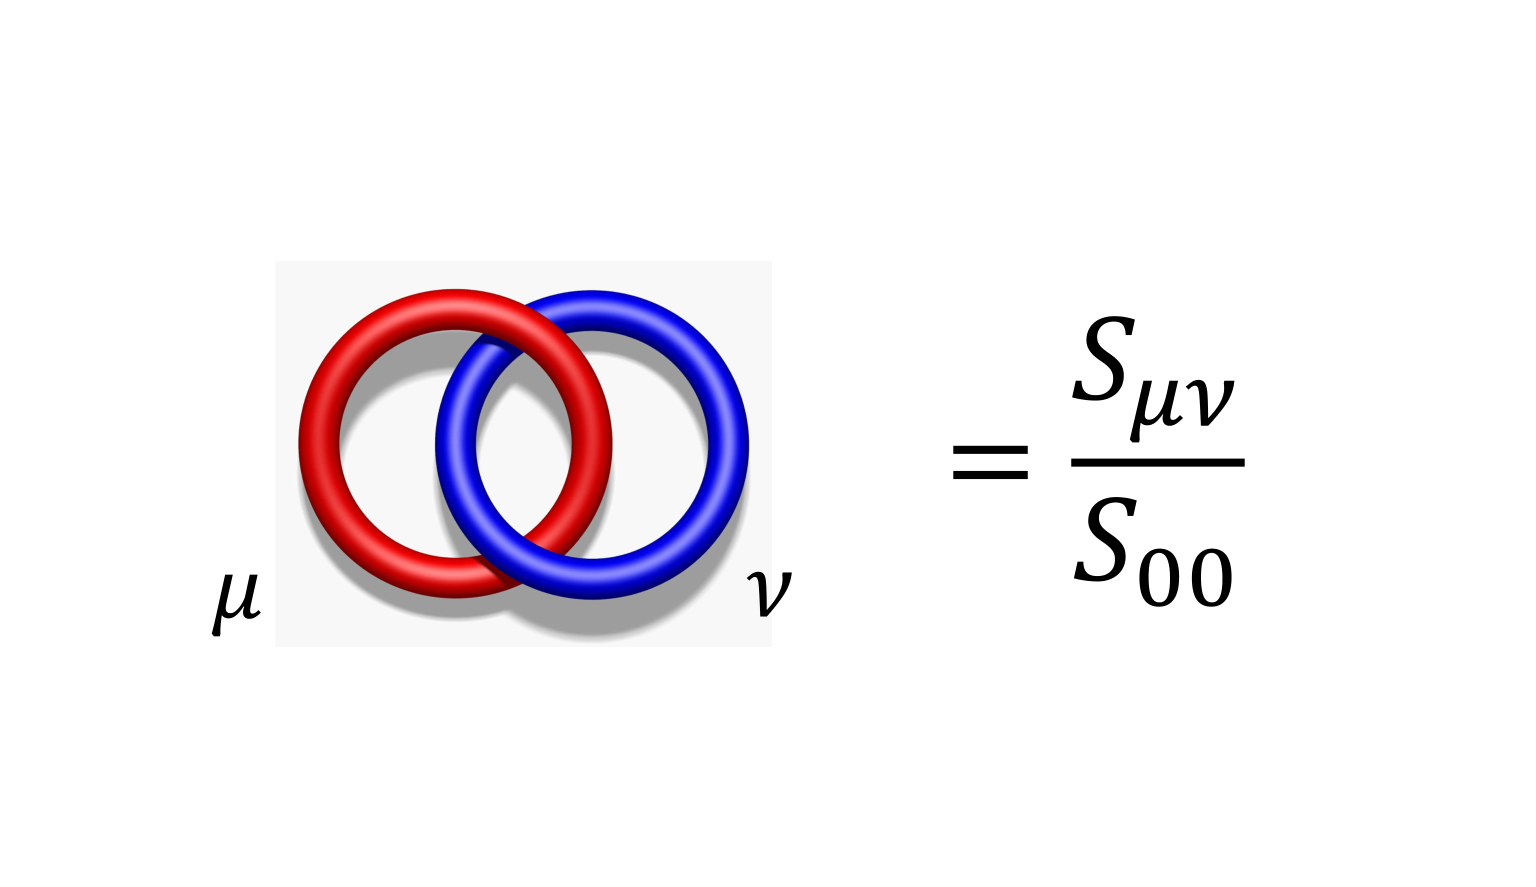
\includegraphics[width=0.60\textwidth]{figures/fig10.png}
  \caption{两条相互链接的圆环，其上分别承载电荷为 $\mu$、$\nu$ 的 Wilson 线缺陷，除此之外不链接任何别的东西；它们等价于一个标量，而这个标量正是模变换 $S$ 在 $\mathcal{H}(T^2)$ 的典范基下的矩阵元 $S_{\mu\nu}$。（原文 Fig.~10，第 72 页）}
  \label{fig:10}
\end{figure}

\begin{enumerate}[start=3]
  \item \underline{与模 $S$ 矩阵的关系。} 特别令人感兴趣的是把关联函数与模 $S$ 矩阵联系起来的一个恒等式。
\end{enumerate}

{\small\itshape ［原文标记：此处已经可以注意到相互链接的圆与模 $S$ 矩阵之间的关系。］}
% [原文待办标记，原文 p.72；其下另有一行星号分隔线，为作者分隔草稿段落所用]

\subsection{与有理共形场论的关系} % 原文: 2.3 Relation To Rational Conformal Field Theory

\subsubsection{\texorpdfstring{$\partial\Sigma$}{∂Σ} 非空时的量子化：边缘态的出现} % 原文: 2.3.1 Quantization When ∂Σ Is Nonempty: Emergence Of Edge States

我们继续考虑 $U(1)$ 能级 $k$ 的 Chern-Simons 理论的量子化。

本节考虑 $M_3=D_2\times\mathbb{R}$，其中 $D_2$ 是一个圆盘。此时出现了边界，因此必须选取边界条件。

一条非常普遍的原则是：\emph{边界条件应当选得使作用量的驻定性成为一个适定的问题。}

换言之，作用量的边界变分应当为零。

{\small\itshape ［原文标记：或许可以用非常一般的辛路径积分来说明，这总归意味着选取一个 Lagrange 子流形。］}
% [原文待办标记，原文 p.72]

在我们的情形中，
\begin{equation}
  \delta\int_{M_3}AdA=\int_{M_3}2\,\delta A\,F+\int_{M_3}d(\delta A\,A)
  \tag{2.299}
  \label{eq:2.299}
\end{equation}
% [Tutor Note: (2.299) 用的是 $\delta(AdA)=\delta A\,dA+A\,d\,\delta A$，第二项分部积分给出恰当形式 $d(\delta A\,A)$，再用 $F=dA$ 把两块合并成 $2\,\delta A\,F$。这里的因子 2 与「无 $\operatorname{tr}$、无 $1/2$」的 $u(1)$ 约定绑定；换到非阿贝尔情形时边界项是 $-\operatorname{tr}(A\,\delta A)$ 型（与 (1.6) 对照），符号与因子都会随之改变，务必统一到 (1.6) 的约定再核对。]

因此我们的边界条件必须使得
\begin{equation}
  \int_{\partial M_3}\delta AA=0
  \tag{2.300}
  \label{eq:2.300}
\end{equation}

最直截了当的做法是在局部强加 $\delta AA|_{\partial M_3}=0$。

在圆盘上取极坐标 $(r,\phi)$，并令 $x^0$ 为时间方向，于是
\begin{equation}
  \delta AA=(\delta A_\phi A_t-\delta A_t A_\phi)\,d\phi\wedge dx^0
  \tag{2.301}
  \label{eq:2.301}
\end{equation}

接下来，我们必须仔细地声明规范变换群是什么。我们把 $A_0$ 视作 Lagrange 乘子，它在 $M_3$ 上强制 $F=0$。于是剩下的规范群只涉及与时间无关的规范变换。

一个有趣的选择是考虑
\begin{equation}
  \mathcal{G}=Map\left(g:D_2\to U(1)\ \middle|\ g|_{\partial D_2}=1\right\}
  \tag{2.302}
  \label{eq:2.302}
\end{equation}
% 原 (2.302) 的定界符本身不配对：左端是圆括号 "("，右端却是花括号 "}"。此处照原样保留（用 \left( ... \right\} 实现），仅加注不加改。
{\small\itshape ［原文标记：这条注记放在这里可能不合适。］}

\textbf{注记}：一般地，若 $X$ 是带边流形，我们考虑群
\begin{equation}
  Map(X\to G)
  \tag{2.303}
  \label{eq:2.303}
\end{equation}
则其中存在由满足 $g|_{\partial X}=1$ 的映射 $g:X\to G$ 组成的子群。在规范场论中，这个子群常被取作描述我们对局部物理之参数化中冗余性的\underline{局部规范变换}群。它是 $Map(X\to G)$ 的正规子群，其商群常被等同于\underline{整体规范变换}群。我们预期态与算符按该群的（可能为射影的）表示变换。

在本情形中可以直截了当地证明 $A_s=ig^{-1}dg=dX$，其中 $X$ 是周期标量场，并且作用量的值只依赖于 $X$ 在边界上的限制：
\begin{equation}
  \int_{D_2\times\mathbb{R}}A_s\partial_0A_s\,dx^0
  =\int_{D_2\times\mathbb{R}}d_s\,(A_s\partial_0X)
  =\int_{\partial D_2\times\mathbb{R}}\partial_\phi X\partial_0X
  \tag{2.304}
  \label{eq:2.304}
\end{equation}
% [Tutor Note: 从 (2.304) 第一式到第二式的关键一步是 $A_s=\partial_sX$（由 $A_s=ig^{-1}\partial_s g=\partial_sX$ 而来），于是 $A_s\partial_0A_s=\tfrac12\partial_0(\partial_sX)^2$；要对 $x^0$ 作一次分部积分（并假定时间方向无边界贡献），才把体积分化为 $\partial D_2\times\mathbb{R}$ 上的边界积分。原文省略了这一步与相应的 $1/2$。此外 $d_s$ 表示只对 $s$ 方向取外微分，别与全微分 $d$ 混用。]

现在让我们回到边界条件，但用 $X$ 来表达它们。我们有
\begin{equation}
  \partial_\phi\delta X\,\partial_tX-\partial_t\delta X\,\partial_\phi X=0
  \tag{2.305}
  \label{eq:2.305}
\end{equation}
若 $X$ 是手征（或反手征）标量场，即可解出
\begin{equation}
  \partial_\phi X\pm\partial_t X=0
  \tag{2.306}
  \label{eq:2.306}
\end{equation}
其中两者取其一，而不可同时取。

{\small\itshape ［原文标记：要提及自对偶场的作用量问题。］}
% [原文待办标记，原文 p.73]

\begin{enumerate}
  \item 如我们所见，在闭三维流形 $M_3$ 上，规范场的 Chern-Simons 不变量 $\frac{1}{4\pi^2}\int_{M_3}AdA$ 的取值只有作为 $\mathbb{R}/\mathbb{Z}$ 的元素才有意义。当 $M_3$ 有非空边界时，情况不同且更为微妙：作用量的值定义了线丛的一个截面。

  {\small\itshape ［原文标记：在这里解释，还是放到后面？？？］}

  \item 反常抵消。我们可以把任意系统与边缘耦合，只要给它配上适当的规范反常，就能得到无反常的系统。
\end{enumerate}

\subsubsection{Wilson 线穿过空间曲面时的量子化} % 原文: 2.3.2 Quantization With Wilson Lines Piercing Spatial Surface

圆盘 $\times\,\mathbb{R}$ 上带 Wilson 线：非平凡和乐。

Gauss 定律中的源。

\subsection{高斯模型：$R^2$ 取有理值的情形} % 原文: 2.4 The Gaussian Model For R^2 Rational

\emph{高斯模型}（Gaussian model）是一个常被用来指代单个无质量标量场（带周期等同）的共形场论的术语。

本节在某种程度上是对共形场论某些简单方面的快速巡览。更详尽的讲述参见：

{\small\itshape ［原文标记：参考文献：Polchinski 第 1 卷；DiFrancesco 等；Fuchs；……？］}
% [原文待办标记，原文 p.74：作者尚未填写的文献指引]

该模型的作用量为
\begin{equation}
  S=K\int dX*dX=K\int d\tau\int_0^{2\pi}d\sigma\left[(\partial_\tau X)^2-(\partial_\sigma X)^2\right]
  \tag{2.307}
  \label{eq:2.307}
\end{equation}
其中 $X$ 无量纲且是周期的（周期可以任意，只要固定下来即可），$K$ 是正常数。

二维的 Green 函数是 $\frac{1}{4\pi}\log|z_1-z_2|^2$，因此
\begin{equation}
  \begin{aligned}
    \langle X(z_1)X(z_2)\rangle&=\frac{1}{2\pi K}\log|z_1-z_2|^2\\
    \langle\partial X(z_1)\partial X(z_2)\rangle&=-\frac{1}{2\pi K}\frac{1}{(z_1-z_2)^2}\,dz_1\wedge dz_2\\
    \langle\bar\partial X(z_1)\bar\partial X(z_2)\rangle&=-\frac{1}{2\pi K}\frac{1}{(\bar z_1-\bar z_2)^2}\,d\bar z_1\wedge d\bar z_2
  \end{aligned}
  \tag{2.308}
  \label{eq:2.308}
\end{equation}

物理学中一种标准的归一化是取 $X\sim X+2\pi$ 以及 $K=\frac{r^2}{4\pi\ell_s^2}$。此时 $X$ 是世界面到半径为 $r$ 的单个圆的映射，而 $\ell_s$ 是弦长。

由运动方程的一般解所定义的高斯场的动量零模与缠绕零模为
\begin{equation}
  X=x_0+\frac{p_L}{\sqrt2}(\tau+\sigma)+\frac{p_R}{\sqrt2}(\tau-\sigma)+X^{\mathrm{osc}}
  \tag{2.309}
  \label{eq:2.309}
\end{equation}
其中我们已取 $\ell_s=1$，$X^{\mathrm{osc}}$ 是非零 Fourier 模的解之和。零模具有这样的性质：向量 $(p_L,p_R)$ 取值于嵌入 $\mathbb{R}^{1,1}$ 的一个偶幺模格中。零模构成的格可写为
\begin{equation}
  \Gamma(r):=\{ne_r+wf_r\,|\,n,w\in\mathbb{Z}\}\subset\mathbb{R}^{1,1}
  \tag{2.310}
  \label{eq:2.310}
\end{equation}
其中
\begin{equation}
  e_r=\frac{1}{\sqrt2}(1/r;1/r),\qquad f_r=\frac{1}{\sqrt2}(r;-r)
  \tag{2.311}
  \label{eq:2.311}
\end{equation}
% [Tutor Note: (2.311) 里的分号 「$;$」 是 Lorentz 型内积下左右手征分量的分隔符，$(v^L;v^R)$ 这种写法与 (2.310) 中 $\mathbb{R}^{1,1}$ 的内积配套。由 $e_r\cdot f_r=1$、$e_r^2=f_r^2=0$ 可验证 $(ne_r+wf_r)^2=2nw$（此处 $p^2=p_L^2-p_R^2$）；若把分号误读成逗号，或误以为 $\{e_r,f_r\}$ 是正交归一对，就会得到 $e_r\cdot f_r=0$ 与 $p^2=n^2+w^2$ 的错误结论。]

注意 $e_r^2=f_r^2=0$、$e_r\cdot f_r=1$，因此 $\Gamma(r)$ 确实是秩 2、符号差 $(1,1)$ 的偶幺模（又称自对偶 Lorentz 型）格 $II^{1,1}$ 的一个嵌入。

该模型具有由流生成的 $u(1)_L\oplus u(1)_R$ 流代数
\begin{equation}
  J_L=\sqrt{\kappa}\sum_{n\in\mathbb{Z}}\alpha_nz^{-n}\frac{dz}{z},
  \qquad
  J_R=\sqrt{\kappa}\sum_{n\in\mathbb{Z}}\tilde\alpha_n\bar z^{-n}\frac{d\bar z}{\bar z}
  \tag{2.312}
  \label{eq:2.312}
\end{equation}
{\small\itshape ［原文标记：这里少了几个恼人的因子 2。］}

我们有
\begin{equation}
  J_L\sim-i\partial X\,\qquad J_R\sim-i\bar\partial X
  \tag{2.313}
  \label{eq:2.313}
\end{equation}
{\small\itshape ［原文标记：恼人的是，在我们的约定下这里有一个非零常数。］}

{\small\itshape ［原文标记：需要对「手征代数」的含义给出更仔细、更形式的讨论。］}
% [原文待办标记，原文 p.75]

它们生成的「手征代数」是由这些场生成的最小的算符乘积代数。忽略左右移动场收缩可能带来的接触项后，我们得到若干个「$u(1)$ 手征代数」的直和。所有这些场都由 $X$ 的（反）全纯导数的多项式得到。我们把它记作 $\mathcal{A}(u(1))$。

{\small\itshape ［原文标记：在此给出手征代数的一般定义；或者推迟，只说这是后面才定义的「手征代数」的一个特例？］}

我们在径向量子化下、于 $SL(2)\times SL(2)$ 不变的真空里计算两点函数：\footnote{这对应于标准归一化
\begin{equation}
  \langle\partial x(z_1)\partial x(z_2)\rangle=-\frac{1}{(z_1-z_2)^2}
  \tag{2.314}
  \label{eq:2.314}
\end{equation}}
\begin{equation}
  \begin{aligned}
    \langle0|J_L(z_1)J_L(z_2)|0\rangle
    &=\kappa\sum_{n=1}^{\infty}n\left(\frac{z_2}{z_1}\right)^{n}\frac{dz_1}{z_1}\otimes\frac{dz_2}{z_2}\\
    &=\frac{\kappa}{(z_1-z_2)^2}\,dz_1\otimes dz_2
  \end{aligned}
  \tag{2.315}
  \label{eq:2.315}
\end{equation}
% [Tutor Note: (2.315) 由级数到闭式用的是一行求和 $\sum_{n\ge1}nx^n=x/(1-x)^2$。取 $x=z_2/z_1$ 得 $\kappa\,z_1z_2/(z_1-z_2)^2$，再乘上 $dz_1/z_1\otimes dz_2/z_2$，两个因子 $z_1z_2$ 恰好相消，才得到最后一行。这也是「必须先设 $|z_1|>|z_2|$ 使级数收敛、再解析延拓」的原因：闭式本身在 $\mathbb{C}\times\mathbb{C}-\mathit{Diag}$ 上单值，但级数不是。]

注意，在径向量子化中我们先在 $|z_1|>|z_2|$ 的区域工作，以使级数收敛；随后由此作解析延拓。对流而言，存在到整个空间 $\mathbb{C}\times\mathbb{C}-\mathit{Diag}$ 的单值解析延拓，没有单值性。

径向量子化中所有关联函数就是这样定义的：理论中的算符要使得关联函数是单值的。

任何手征代数都含有 $T(z)$ 及其全部导数与导数的乘积。注意在此情形
\begin{equation}
  T(z)=-\frac12(\partial x)^2=\frac{1}{2\kappa}:J_L^2:
  \tag{2.316}
  \label{eq:2.316}
\end{equation}
这称为能动张量的 \emph{Sugawara 形式}，它在非阿贝尔情形下将以略微修改的形式成立。

{\small\itshape ［原文标记：$U(1)$ 手征代数的幺正表示（以下为作者以星号框出的草稿段落）：］}
% [原文待办标记，原文 p.76：星号框内的草稿小节，尚未并入正文]

表示：$V_p$，$p\in\mathbb{C}$。幺正表示：$p\in\mathbb{R}$。特征标
\begin{equation}
  \begin{aligned}
    \chi_p&:=\operatorname{Tr}_{V_p}q^{L_0-\frac{c}{24}}e^{2\pi i\xi J_0}\\
    &=\frac{q^{\frac12p^2}e^{2\pi i\xi p}}{\eta}
  \end{aligned}
  \tag{2.317}
  \label{eq:2.317}
\end{equation}

此外，该模型还有顶点算符
\begin{equation}
  V_p(z,\bar z)=c(p):e^{ip_LX(z)}\otimes e^{ip_R\tilde X(\bar z)}:
  \tag{2.318}
  \label{eq:2.318}
\end{equation}
其中动量 $p=(p_L;p_R)$ 被限制在偶幺模格 $\Gamma(r)$ 之中。于是
\begin{equation}
  \begin{aligned}
    p_L&=\frac{1}{\sqrt2}\left(\frac{n}{r}+wr\right)\\
    p_R&=\frac{1}{\sqrt2}\left(\frac{n}{r}-wr\right)
  \end{aligned}
  \tag{2.319}
  \label{eq:2.319}
\end{equation}
其中 $n,w\in\mathbb{Z}$ 分别是动量量子数与缠绕量子数。{\small\itshape ［原文标记：（此处 $c(p)$ 是一个「余闭链算符」——是忽略它，还是解释它？）］} 我们标出了标准的正规序符号。此后我们假定所有取指数形式的顶点算符都带有这一正规序，并在记号中略去不写。

这些场的算符乘积恰好是：
\begin{equation}
  V_{p_1}(1)V_{p_2}(2)=\varepsilon(p_1,p_2)(z_1-z_2)^{p_1^L\cdot p_2^L}(\bar z_1-\bar z_2)^{p_1^R\cdot p_2^R}c(p_1,p_2):e^{i(p_1^LX_L(1)+p_2^LX_L(2))}\otimes e^{i(p_1^RX_R(1)+p_2^RX_R(2))}
  \tag{2.320}
  \label{eq:2.320}
\end{equation}
这里余闭链算符满足 $c(p_1)c(p_2)=\varepsilon(p_1,p_2)c(p_1+p_2)$。它们定义了格 $\Gamma(r)$ 的一个 $\mathbb{Z}_2$ 中心扩张，也就是说，$\varepsilon(p_1,p_2)$ 取值于 $\{\pm1\}$，并且必须满足
\begin{equation}
  \frac{\varepsilon(p_1,p_2)}{\varepsilon(p_2,p_1)}=(-1)^{p_1\cdot p_2}
  \tag{2.321}
  \label{eq:2.321}
\end{equation}
% [Tutor Note: (2.321) 只是 $\varepsilon$ 的相容性条件，它并不能唯一确定 $\varepsilon$；而 (2.320) 中 $\varepsilon(p_1,p_2)$ 与 $c(p_1,p_2)$ 同时出现，正文只说 $c(p_1)c(p_2)=\varepsilon(p_1,p_2)c(p_1+p_2)$，两者的相对归一化（是否把 $\varepsilon$ 吸收进 $c$ 的定义）原文并未固定。计算多顶点关联函数时必须自始至终用同一套约定，否则结果会差出 $\pm1$ 的相位。]

{\small\itshape ［原文标记：解释：］}
\begin{enumerate}
  \item 它是单值的，因为 $p_1\cdot p_2\in\mathbb{Z}$，因为 $\Gamma(r)$ 是整格。
  \item 从而，利用径向量子化与 $SL(2,\mathbb{R})\times SL(2,\mathbb{R})$ 不变的真空：
  \begin{equation}
    \langle\prod_iV_{p_i}(z_i,\bar z_i)\rangle
    =\mathcal{F}_L(z_1,\dots,z_N)\tilde{\mathcal{F}}_R(\bar z_1,\dots,\bar z_N)
    \tag{2.322}
    \label{eq:2.322}
  \end{equation}
  其中
  \begin{equation}
    \mathcal{F}_L(z_1,\dots,z_N)=\prod_{i<j}(z_i-z_j)^{p_i^Lp_j^L}
    \tag{2.323}
    \label{eq:2.323}
  \end{equation}
  被称为该关联函数的\emph{共形块}。
  \item 强调：关联函数是单值的，但共形块具有非平凡的单值性。
\end{enumerate}

对特殊半径，某些 $V_{p_L,p_R}$ 会成为纯全纯算符。这发生在丢番图方程 $p_R=0$ 有解之时。显然这要求
\begin{equation}
  r^2=\frac{m}{w}
  \tag{2.324}
  \label{eq:2.324}
\end{equation}
对某些整数 $m,w$ 成立，因而 $r^2\in\mathbb{Q}$。这些模型称为\emph{有理高斯模型}。它们属于最简单的有理共形场论之列。

{\small\itshape ［原文标记：同样：是否要给出 RCFT 的形式定义？还是推迟？］}

于是，设 $r^2=p/q$ 为既约有理数。则全纯算符由 $m=\ell p$ 与 $w=\ell q$ 得到。它们都是基本全纯顶点算符的各次幂：
\begin{equation}
  V_\pm:=c_\pm e^{i\sqrt{2pq}X}
  \tag{2.325}
  \label{eq:2.325}
\end{equation}
令 $\kappa=pq$。则这些算符具有整数共形维数 $\kappa$，并且绕由 $J_L(z)$ 生成的算符没有单值性，因此可以把它们加到手征代数 $\mathcal{A}(u(1))$ 上，得到更大的手征代数，称为 $u(1)$ 能级 $\kappa$ 手征代数，记作 $\mathcal{A}(u(1))_\kappa$。

$\mathcal{A}(u(1))_\kappa$ 的表示可以在半径 $r^2=p/q$ 处高斯模型顶点算符的全纯部分中找到。它们由「手征顶点算符」生成：
\begin{equation}
  V_n(z)=c\,e^{i\frac{n}{\sqrt{2\kappa}}X(z)}
  \tag{2.326}
  \label{eq:2.326}
\end{equation}

\textbf{警告}：式 \eqref{eq:2.326} 的逻辑地位与 \eqref{eq:2.325} 有重要不同。\eqref{eq:2.326} 中的场本身并不属于高斯模型的谱。左移部分与右移部分必须组合成单值的非全纯场。这与 \eqref{eq:2.325} 相当不同：后者这些场是位于理论的谱中的。

注意 $n\sim n+2\kappa$，而特征标为
\begin{equation}
  \begin{aligned}
    \chi_n(z,\tau)&:=\operatorname{Tr}_{H_n}q^{L_0-\frac{c}{24}}e^{2\pi i\xi J_0}\\
    &=\frac{\sum_{\ell\in\mathbb{Z}}q^{\frac12p_L^2}e^{2\pi i\xi p_L}}{\eta}\\
    &=\frac{\sum_{\ell\in\mathbb{Z}}e^{2\pi i\kappa\tau\left(\ell+\frac{n}{2\kappa}\right)^2+2\pi iz(2\ell\kappa+n)}}{\eta}\\
    &=\frac{\Theta_{n,\kappa}(z,\tau)}{\eta}
  \end{aligned}
  \tag{2.327}
  \label{eq:2.327}
\end{equation}
其中我们定义了 $z=\xi/\sqrt{2\kappa}$，作为在处理模变换与周期性时更方便的归一化。

现在让我们考虑把左移与右移结合起来的 RCFT 的配分函数。在一般半径处我们有
\begin{equation}
  \begin{aligned}
    \operatorname{Tr}_{\mathcal{H}}e^{2\pi i\tau(L_0-\frac{c}{24})+i\xi J_0-2\pi i\bar\tau(\tilde L_0-\frac{\tilde c}{24})-2\pi i\tilde\xi\tilde J_0}
    &=\frac{\sum_{(p_L,p_R)\in\Gamma(r)}q^{\frac12p_L^2}\bar q^{\frac12p_R^2}e^{2\pi i\xi p_L-2\pi i\tilde\xi p_R}}{\eta\bar\eta}\\
    &=\sum_{(p_L,p_R)\in\Gamma(r)}\chi_{p_L}(z,\tau)\overline{\chi_{p_R}(z,\tau)}
  \end{aligned}
  \tag{2.328}
  \label{eq:2.328}
\end{equation}

现在，这个表达式也可以解释为环面上的路径积分：
\begin{equation}
  Z(\tau,\xi;\bar\tau,\bar\xi)
  =e^{-2\frac{(\operatorname{Im}\xi)^2}{\operatorname{Im}\tau}}\operatorname{Tr}_{\mathcal{H}}e^{2\pi i\tau(L_0-\frac{c}{24})+i\xi J_0-2\pi i\bar\tau(\tilde L_0-\frac{\tilde c}{24})-2\pi i\tilde\xi\tilde J_0}
  \tag{2.329}
  \label{eq:2.329}
\end{equation}
其中
\begin{equation}
  Z(\tau,\xi;\bar\tau,\bar\xi)=\int[dX]\,e^{-K\int_\Sigma(\partial X+A^{1,0})\wedge(\bar\partial X+A^{0,1})}
  \tag{2.330}
  \label{eq:2.330}
\end{equation}
并且我们耦合了平坦外场规范场 $A=a_1d\sigma^1+a_2d\sigma^2$，以及
\begin{equation}
  \xi=\mathit{constant}\,\frac{1}{2\pi}(a_2-\bar\tau a_1)
  \tag{2.331}
  \label{eq:2.331}
\end{equation}

该路径积分显然是微分同胚不变的，并且在外场、非动力学 $U(1)$ 规范场 $A$ 的规范变换下是规范不变的。
{\small\itshape ［原文标记：需要核对此式！］}

当一个与度规和/或规范场耦合的路径积分不能适当地规范不变时，我们说存在\emph{反常}。由于我们以对称的方式耦合了左移与右移玻色子，此情形下不可能出现反常。

{\small\itshape ［原文标记：在此给出路径积分计算的细节：］}
\begin{enumerate}
  \item 相关场空间并不连通，且有拓扑上不同的扇区：$X=X_q+X_{sol}$，其中 $X_{sol}=2\pi n^1\sigma^1+2\pi n^2\sigma^2$，$n^1,n^2\in\mathbb{Z}$。
  \item 于是 $Z=Z_q\sum_{n,m}e^{-S_{\mathrm{class}}}$。

  {\small\itshape ［原文标记：给出经典作用量的公式］}

  \item 对 $m$ 作 Poisson 重求和。
  \item 用 $\zeta$ 函数正则化计算 $Z_q$，得到
  \begin{equation}
    Z_q=\frac{1}{\sqrt{\operatorname{Im}\tau}\,|\eta(\tau)|^2}
    \tag{2.332}
    \label{eq:2.332}
  \end{equation}
  \item 评注：对非紧致玻色子我们有
  \begin{equation}
    Z_q=\frac{1}{\sqrt{\operatorname{Im}\tau}\,|\eta(\tau)|^2}
    \tag{2.333}
    \label{eq:2.333}
  \end{equation}
  这可以从 $r\to\infty$ 极限恢复：它来自 Gauss 积分
  \begin{equation}
    \int_{-\infty}^{+\infty}dp\,e^{-\pi\operatorname{Im}\tau\,p^2}
    \tag{2.334}
    \label{eq:2.334}
  \end{equation}
\end{enumerate}
% [Tutor Note: (2.332) 与 (2.333) 的右端逐字相同，这很可能是原稿的笔误，也可能是作者有意强调「两种情形的振荡子行列式部分一致」。(2.333) 的语境是 $r\to\infty$ 的非紧致极限，其额外的动量积分正是 (2.334)；因此 (2.333) 里的 $Z_q$ 应理解为振荡子部分，而非完整的非紧致配分函数。引用时不要由此推断紧致与非紧致玻色子的配分函数相等。]

{\small\itshape ［原文标记：（星号框结束线）］}

现当 $r^2=p/q$ 时，对 Narain 格 $\Gamma(r)$ 的无穷求和会以有趣的方式简化
% 原句在印刷页 p.78 末尾被截断，续见下一片段；此处不补句号，以免造成「句子已完」的错觉。

% 本片段自印刷页 p.79 顶部接续上一片段末句（"……会以有趣的方式简化"），原文在此直接给出编号公式 (2.335)。

\begin{equation}
  Z(z,\tau;\bar z,\bar\tau)
  = e^{-4\pi k\,\frac{(\operatorname{Im}z)^2}{\operatorname{Im}\tau}}
  \sum_{r,\tilde r\in\mathbb{Z}/2k\mathbb{Z}}
  D_{r,\tilde r}\,\chi_r(z,\tau)\,\overline{\chi_{\tilde r}(z,\tau)}
  \tag{2.335}
  \label{eq:2.335}
\end{equation}
% [Tutor Note: (2.335) 的前因子指数是 $(\operatorname{Im}z)^2/\operatorname{Im}\tau$，不是 $|z|^2$ 也不是 $z\bar z$：它来自环面上与 $z$ 相关的零模方向的高斯积分，故与 $\tau$ 的虚部绑定。上划线只覆盖右移因子 $\chi_{\tilde r}$，作者并没有把它写成 $|\chi_r|^2$，因为左移指标 $r$ 与右移指标 $\tilde r$ 一般并不相等；把 (2.335) 与 (2.328) 并排对照时，最容易错的就是这一点。]

矩阵 $D_{r,\tilde r}$ 将在下文第 2.4.1 节中进一步讨论。

由上述计算我们可以得出若干重要结论：

\begin{enumerate}
  \item 在 \eqref{eq:2.328} 与 \eqref{eq:2.335} 两式中，我们都看到共形场论的典型特征：配分函数是若干「全纯对象乘以反全纯对象」之和，至多差一个简单的局部因子。注意它们对 $z$ 与 $\tau$ 都是全纯的。这些全纯因子称为\emph{共形块}（conformal blocks），而\emph{有理}共形场论的一条（定义性的）性质是：所有黎曼面上的所有关联函数都是这样的和。该局部前因子代表了在同时要求规范不变性与全纯分解时所出现的\emph{反常}（anomaly）。这一观察至少可以追溯到 [5]。

  {\small\itshape ［原文标记：确实需要讨论模变换，才能看出真正不变的东西只是共形块构成的向量空间。］}
  % [原文待办标记，原文 p.79；位于页边竖排]

  \item 再者，作为 $z$ 的函数，共形块的向量空间与 $U(1)_k$ Chern-Simons 理论的 Hilbert 空间相同。这将成为一个普遍原理：

  \begin{quote}
    \itshape
    在 $\Sigma\times\mathbb{R}$ 上量子化的 Chern-Simons 规范理论中，物理态的向量空间，与相应的有理共形场论的共形块空间之间存在同构。此外，若该 Chern-Simons 理论是借助由 $\Sigma$ 上某个复结构的选择所诱导的 Kähler 量子化来量子化的，则这乃是黎曼面模空间上全纯向量丛之间的等同。
  \end{quote}

  我们的目标之一，就是在更一般的 Chern-Simons 理论的背景下更好地理解这一陈述。

  \item 在这个意义上，带边的三维流形上的拓扑 Chern-Simons 理论与边界上的（有理共形场论的手征一半）之间存在某种等价。这是一种「全息」（holography）。
\end{enumerate}

\subsubsection{把同一手征代数粘合出不同半径} % 原文: 2.4.1 Gluing The Same Chiral Algebra To Get Different Radii

爱钻研的读者会注意到，整数 $k$ 可以有多种分解 $k=pq$（即使 $k$ 是素数时也是如此）。那么是什么挑出了不同的半径？

\underline{在 RCFT 框架内的回答}

在 \eqref{eq:2.335} 中，矩阵 $D_{r,r'}$ 告诉我们如何把左移与右移部分粘合起来。如 [43] 所示，这必须通过 $\mathbb{Z}/(2k\mathbb{Z})$ 融合规则代数的一个自同构来完成。（这是关于 RCFT 中表示粘合的一般性结果。）把该阿贝尔群按加法来想，自同构就是 $x\mapsto yx$，其中 $y$ 与 $2k$ 互素。[43] 中声称：若取基本区 $0\le r\le 2k-1$，则当 $r=pr_2+qr_1$、$r'=qr_1-pr_2$，而 $(r_1,r_2)$ 取值于 $\mathbb{Z}\oplus\mathbb{Z}$ 中由 $(\pm p,0)$ 与 $(0,\pm q)$ 所决定的菱形区域时，$D_{r,r'}=1$。

{\small\itshape ［原文标记：最好再核对一遍。有一篇 Dijkgraaf–Verlinde 的相关论文，需要引用。］}
% [原文待办标记，原文 p.80；位于页边竖排]
% [Tutor Note: 作者自己在页边写了「最好再核对一遍」，说明 $D_{r,r'}$ 的这条「菱形区域」判据在原稿中尚未最终定稿。它的含义是把融合规则代数的自同构 $x\mapsto yx$ 图解化：$r\mapsto r'$ 必须是该自同构诱导的置换，而菱形区域只是保证 $(r_1,r_2)\mapsto(pr_2+qr_1,\,qr_1-pr_2)$ 在其中单值。引用 $D_{r,r'}$ 的具体形式（例如计算某个 $k=pq$ 下的显式矩阵）之前，务必先用 $\gcd(y,2k)=1$ 核对它确实是双射。]

\underline{在 Maxwell-Chern-Simons 理论框架内的回答}

正如 [26] 中所详加讨论的，在 Chern-Simons 理论的框架内导出最低 Landau 能级（lowest Landau level, LLL）波函数，实际上会挑出一个优先的半径。让我们回到 \eqref{eq:2.199}，把 LLL 中波函数的公式代入。我们得到：
\begin{equation}
  \bar\Psi(A) := \mathcal{N}\,e^{-4\pi k\operatorname{Im}\tau\,A_zA_{\bar z}}
  \sum_{\omega\in\mathcal{H}^1_{\mathbb{Z}}}
  e^{-4\pi k\operatorname{Im}\tau\,\omega_z\omega_{\bar z}}
  e^{-8\pi k\operatorname{Im}\tau\,\omega_{\bar z}A_z}
  \,\psi(A_z+\omega_z)
  \tag{2.336}
  \label{eq:2.336}
\end{equation}
% [Tutor Note: 求和指标 $\omega$ 属于 $\mathcal{H}^1_{\mathbb{Z}}$，即整系数上同调类所标记的大平移/大动量扇区。指数里 $\omega_z\omega_{\bar z}$ 与 $\omega_{\bar z}A_z$ 的系数分别是 $4\pi k$ 与 $8\pi k$，比值 $1:2$ 正是把二次型在 $A+\omega$ 处展开后交叉项的系数；把 (2.336) 与 (2.199) 对照或做配方时若丢掉这个 $1:2$，就得不到正确的半径。]

我们能认出来，这是某个周期标量场（同时含左移与右移自由度）在某个\underline{特定半径}处的瞬子求和，即
\begin{equation}
  S=\frac{k}{4\pi}\int d\phi*d\phi
  \tag{2.337}
  \label{eq:2.337}
\end{equation}
其中 $\phi\sim\phi+2\pi$，并与 $A^{1,0}$ 有手征耦合：
\begin{equation}
  2ik\int\bar\partial\phi\wedge A^{1,0}
  \tag{2.338}
  \label{eq:2.338}
\end{equation}

我们可以通过把环面上该玻色子（作用量为上式）的配分函数与 \eqref{eq:2.336} 对照，来解读这一信息。半径为 $r^2=k\ell_s^2$。进一步的讨论（包括向环面规范群的非凡推广）见 [26]。

\underline{在拓扑场论框架内的回答：面缺陷}

融合规则的非平凡自同构，可以解释为在三维理论中定义\emph{面缺陷}（surface defects）。见 [35]。

{\small\itshape ［原文标记（星号框）：关于 Kapustin–Saulina 的图景，需要再多解释一些。］}
% [原文待办标记，原文 p.80]

\subsubsection{自由费米子半径：能级 1/2 的 theta 函数与环面上的旋量结构} % 原文: 2.4.2 The Free Fermion Radius: Level 1/2 Theta Functions And Spin Structures On The Torus

从 \eqref{eq:2.310} 可以清楚地看到，有一些特别值得关注的半径：

\begin{enumerate}
  \item 有著名的 $r\to1/r$ T-对偶对称性，因此我们只需考察 $r\ge1$。

  \item 在 $T$-对偶的不动点 $r=1$ 处，存在增强的 $SO(4)=(SU(2)_L\times SU(2)_R)/\mathbb{Z}_2$ 对称性。

  \item 在半径 $r^2=2$ 处，有 $\sqrt{2pq}=2$，于是我们有共形维数为 $1/8$ 的全纯算符 $e^{\pm\frac{i}{2}X_L(z)}$，以及它们的平方
  \begin{equation}
    \psi(z)=e^{iX_L(z)}
    \qquad
    \bar\psi(z)=e^{-iX_L(z)}
    \tag{2.339}
    \label{eq:2.339}
  \end{equation}
  其维数为 $h=1/2$。

  \item 在半径 $k=6$ 处，理论实际上具有 $N=2$ 超对称。$r=\pm6$ 的表示给出
  \begin{equation}
    G^{\pm}(z)\sim e^{\pm i\sqrt{3}X}
    \tag{2.340}
    \label{eq:2.340}
  \end{equation}
  它们惊人地满足 $N=2$ 超共形代数。
\end{enumerate}

最后两个例子启发了引入\emph{超手征代数}的想法。在自由费米子情形，我们有
\begin{equation}
  \begin{aligned}
    \psi(z_1)\psi(z_2) &\sim (z_1-z_2)\,{:}\,\psi(z_1)\psi(z_2)\,{:}\\
    \psi(z_1)\bar\psi(z_2) &\sim (z_1-z_2)^{-1}+{:}\,\partial\psi\,\psi\,{:}+\mathcal{O}(z_1-z_2)
  \end{aligned}
  \tag{2.341}
  \label{eq:2.341}
\end{equation}

于是 $\psi$ 与 $\bar\psi$「几乎」构成一个手征代数：它们的关联函数是单值的，但存在非平凡的编织：关联函数中 $\psi$ 与 $\bar\psi$ 的排序是有影响的。

\begin{enumerate}[start=3]
  \item 无论如何，在这个特殊的「自由费米子半径」处，高斯模型存在一个「双重覆盖」。然而，相当显然地，要定义关联函数我们必须定义旋量结构。

  \item 这或许最明显的例子就在配分函数的计算中。首先，我们必须为
  \begin{equation}
    \psi(z)=\sum d_rz^{-r-1/2}dz^{1/2}
    \tag{2.342}
    \label{eq:2.342}
  \end{equation}
  选取费米子边界条件，其中 $z=e^{i\phi+t}$，视作 $\phi$ 的函数。
  % [Tutor Note: (2.342) 的求和号下原文本就未写出指标范围：NS 扇区取 $r\in\mathbb{Z}+\frac12$，R 扇区取 $r\in\mathbb{Z}$（见本节下一条与附录 G）。此外因子 $dz^{1/2}$ 表明 $\psi$ 是 $\frac12$-微分；在 $z=e^{i\phi+t}$ 这类坐标变换下，半整数权会带来额外的相位，讨论环面边界条件时不能漏掉它。]

  \item 如附录 G 中所解释的，圆上有两种旋量结构，即 Neveu-Schwarz（NS）与 Ramond（R）旋量结构，分别对应于 $\psi$ 的反周期与周期边界条件。用模式展开来说，NS 对应于 $r\in\mathbb{Z}+\frac12$，R 对应于 $r\in\mathbb{Z}$。

  \item $\operatorname{Tr}e^{-\beta H}$ 自然地选取反周期边界条件。[见任何一本 QFT 教科书，或自行验证]。

  \item 总共有四个自然的环面配分函数，对应于环面上的四种旋量结构。（约定：$Z(g_t,g_s;\tau)$ 表示环面上带扭曲边界条件。）

  {\small\itshape ［原文标记：弄个方框宏（box macro）来画带边界条件的环面。］}
  % [原文待办标记，原文 p.81；位于页边竖排]

  \begin{equation}
    \begin{aligned}
      Z(+,+) &= \frac{\vartheta_1(z,\tau)}{\eta(\tau)}\\
      Z(-,+) &= \frac{\vartheta_2(z,\tau)}{\eta(\tau)}\\
      Z(-,-) &= \frac{\vartheta_3(z,\tau)}{\eta(\tau)}\\
      Z(+,-) &= \frac{\vartheta_4(z,\tau)}{\eta(\tau)}
    \end{aligned}
    \tag{2.343}
    \label{eq:2.343}
  \end{equation}

  {\small\itshape ［原文标记：ETC.（等等）］}
  % [原文标记，原文 p.82 首行；作者此处以大写 ETC. 表示「以下同理」，属未写完的列表收尾]

  这里我们引入了半整数能级的 theta 函数。

  定义：

  {\small\itshape ［原文标记：取决于我们在「带电粒子绕环运动」那一节里讲了多少，此处就直接回指那里。］}
  % [原文待办标记，原文 p.82；位于页边竖排]

  \begin{equation}
    \vartheta\left[\genfrac{}{}{0pt}{}{\theta}{\phi}\right](z|\tau)
    := \sum_{n\in\mathbb{Z}}
    e^{i\pi\tau(n+\theta)^2+2\pi i(n+\theta)(z+\phi)}
    \tag{2.344}
    \label{eq:2.344}
  \end{equation}

  \begin{equation}
    \begin{aligned}
      \vartheta_1(z|\tau) &:= \vartheta\left[\genfrac{}{}{0pt}{}{1/2}{1/2}\right](z|\tau)
      = 2q^{1/8}\cos\left[\pi\left(z+\tfrac12\right)\right]+2q^{9/8}\cos\left[3\pi\left(z+\tfrac12\right)\right]+\cdots\\
      \vartheta_2(z|\tau) &:= \vartheta\left[\genfrac{}{}{0pt}{}{1/2}{0}\right](z|\tau)
      = 2q^{1/8}\cos(\pi z)+2q^{9/8}\cos(3\pi z)+\cdots\\
      \vartheta_3(z|\tau) &:= \vartheta\left[\genfrac{}{}{0pt}{}{0}{0}\right](z|\tau)
      = 1+2\cos[2\pi z]\,q^{1/2}+2\cos[4\pi z]\,q^{2}+\cdots\\
      \vartheta_4(z|\tau) &:= \vartheta\left[\genfrac{}{}{0pt}{}{0}{1/2}\right](z|\tau)
      = 1-2q^{1/2}\cos[2\pi z]+2q^{2}\cos[4\pi z]+\cdots
    \end{aligned}
    \tag{2.345}
    \label{eq:2.345}
  \end{equation}
  % [Tutor Note: (2.345) 用的是 Jacobi 的经典约定：$q=e^{2\pi i\tau}$，特征 $\vartheta\bigl[\genfrac{}{}{0pt}{}{\theta}{\phi}\bigr]$ 的上下指标与 $\vartheta_{1},\dots,\vartheta_{4}$ 的对应依次为 $(1/2,1/2)$、$(1/2,0)$、$(0,0)$、$(0,1/2)$。注意 $\vartheta_1$ 的宗量是 $\cos[\pi(z+\frac12)]$ 而 $\vartheta_2$ 是 $\cos(\pi z)$，二者相差一个 $z\to z+\frac12$ 的平移；抄写时最易在此处丢掉 $\frac12$。]

  {\small\itshape ［原文标记：还要给出无穷乘积表示。这些公式都应当放进附录。］}
  % [原文待办标记，原文 p.82；位于页边竖排]

  \item 讨论 $PSL(2,\mathbb{Z})$ 的三个指数为 3 的子群，它们各自保持三种偶旋量结构。用它来解释上述 theta 函数的 $S$ 变换与 $T$ 变换。

  \item 评述自旋算符及其关联函数。
\end{enumerate}

\subsection{旋量理论} % 原文: 2.5 Spin Theories

Chern-Simons 理论的一个重要变体是\emph{旋量 Chern-Simons}（spin-Chern-Simons）理论。在此情形中，$M_3$ 除了定向之外还具有一个\emph{旋量结构}，而 Chern-Simons 作用量确实依赖于该旋量结构。

旋量结构的数学背景见附录 G。

我们可以借助把规范丛配边到零的办法，来定义闭三维流形上的 Chern-Simons 不变量。这意味着我们要找到一个四维流形 $W_4$，使得
\begin{equation}
  \partial W_4=M_3
  \tag{2.346}
  \label{eq:2.346}
\end{equation}
并把丛延拓到 $W_4$ 上。丛一旦可以延拓，由单位分解的论证，延拓联络就没有任何问题。现在，有了这些额外数据，我们就可以把 Chern-Simons 不变量
\begin{equation}
  CS(A)=\frac{1}{(2\pi)}\int_{M_3}AdA\ \in\mathbb{R}/2\pi\mathbb{Z}
  \tag{2.347}
  \label{eq:2.347}
\end{equation}
提升为真正的实数：
\begin{equation}
  \widehat{CS}(A;W_4)=2\pi\int_{W_4}\frac{F}{2\pi}\wedge\frac{F}{2\pi}\ \in\mathbb{R}
  \tag{2.348}
  \label{eq:2.348}
\end{equation}
% [Tutor Note: (2.347) 用的是阿贝尔情形 $U(1)$ 的归一化 $\frac{1}{2\pi}\int A\,dA$（既无 $\operatorname{tr}$，也不是 $\frac{1}{4\pi}$），与非阿贝尔的 (3.7)（$\frac{k}{8\pi^2}\operatorname{tr}$）是两套完全不同的约定；把 (2.354) 的相位因子与 (3.12) 的 Wess-Zumino 型整数对比之前，必须先统一到同一套归一化，否则会莫名其妙地差出因子 2 或 4。]

$W_4$ 的选取可以不同，而这些差别
\begin{equation}
  \left(\widehat{CS}(A;W_4)-\widehat{CS}(A;W'_4)\right)
  =2\pi\int_{Z_4}\frac{F}{2\pi}\wedge\frac{F}{2\pi}\ \in2\pi\mathbb{Z}
  \tag{2.349}
  \label{eq:2.349}
\end{equation}
% 原 (2.349) 把第二个四维流形印作 $W'_r$（下标为 $r$ 而非 $4$），紧随其后的正文又称之为 $W'_4$，这是原稿的排版笔误；此处照原样转写，引用时应按 $W'_4$ 理解。
是某个闭四维流形 $Z_4$（由把 $W_4$ 与 $W'_r$ 粘合（gluging）而得）上，丛的第一 Chern 类的代表元之楔积的积分。这是一个整形式的积分，因而是一个整数。例如，若 $Z_4=\mathbb{CP}^2$ 且 $[F/2\pi]=c_1(H)$，其中 $H$ 是基本的超平面丛（tautological hyperplane bundle），则该整数为 $+1$。

{\small\itshape ［原文标记：评注一下对 $A$ 延拓到 $W_4$ 的方式的依赖。］}
% [原文待办标记，原文 p.82；位于页边竖排]

我们想把这个 CS 作用量除以 2，以定义半整数能级的 Chern-Simons 理论。但这将导致一个定义不良的作用量。上面 $Z_4=\mathbb{CP}^2$ 的例子表明情况确实可能如此。

这「只不过」是一个符号问题，因为我们「只不过」是在取 $\exp[iCS(A)]$ 的平方根；但此处若马虎，会导致严重错误。

$H^2(Z_4;\mathbb{Z})$ 是一个整格。一般地，给定整格 $\Lambda$，满足
\begin{equation}
  v^2=c\cdot v\mod 2
  \tag{2.350}
  \label{eq:2.350}
\end{equation}
的向量 $c$ 称为\emph{特征向量}（characteristic vector）。特征向量总是有无穷多个，而任意两个（比如 $c,c'$）相差一个可被 2 整除的向量，即 $c-c'\in2\Lambda$。当 $c$ 是特征向量时，$\frac12v\cdot(v+c)$ 是整数。

结果表明，$w_2\in H^2(Z_4;\mathbb{Z}_2)$ 的任意整提升 $\widehat{w_2}$ 都是特征向量。这促使我们给出半整数 Chern-Simons 项的定义：

\emph{我们在 $W_4$ 上选取一个旋量结构 $\mathsf{s}$，并令}
\begin{equation}
  \frac12\widehat{CS}(A;W_4;\mathsf{s})
  :=2\pi\int_{W_4}\frac12\frac{F}{2\pi}\wedge\left(\frac{F}{2\pi}+\widehat{w_2}\right)\ \in\mathbb{R}
  \tag{2.351}
  \label{eq:2.351}
\end{equation}

{\small\itshape ［原文标记：你这里用的是 $\widehat{w_2}$。需要说明，同一旋量结构的不同提升无关紧要。］}
% [原文待办标记，原文 p.83；位于页边竖排]
% [Tutor Note: 这里正是作者留待补充的一步。若 $\widehat{w_2}$ 与 $\widehat{w_2}'$ 是 $w_2$ 的两个整提升，则 $\widehat{w_2}-\widehat{w_2}'=2\beta$，其中 $\beta$ 是 $W_4$ 上的整形式；代回 (2.352) 后多出的项为 $2\pi\int_{Z_4}\frac{F}{2\pi}\wedge\beta\in2\pi\mathbb{Z}$，故指数化作用量不变，定义与提升的选取无关。原文把这步留作 "Need to explain"，读者须自行补上。]

现在，若有两个延拓，使得所有数据（包括旋量结构）在公共边界上一致，则
\begin{equation}
  \frac12\widehat{CS}(A;W_4;\mathsf{s})-\frac12\widehat{CS}(A;W'_4;\mathsf{s}')
  =2\pi\int_{Z_4}\frac12\frac{F}{2\pi}\wedge\left(\frac{F}{2\pi}+\widehat{w_2}\right)\ \in2\pi\mathbb{Z}
  \tag{2.352}
  \label{eq:2.352}
\end{equation}
正如所愿。因此我们可以把旋量 Chern-Simons 作用量定义为
\begin{equation}
  \exp\left[2\pi i\frac12CS(A;\mathsf{s})\right]
  :=\exp\left[2\pi\int_{W_4}\frac12\frac{F}{2\pi}\wedge\left(\frac{F}{2\pi}+\widehat{w_2}\right)\right]
  \tag{2.353}
  \label{eq:2.353}
\end{equation}

我们付出的代价是：

\begin{enumerate}
  \item 须把注意力限制在带旋量结构选择的 $W_4$ 上。这不是严重的限制，因为三维的旋量配边群是平凡的，带主 $U(1)$ 丛的旋量流形的配边群亦然。（在更高维，这类限制可能变得相当重要。）

  \item 我们需要把 $w_2$ 的一个显式提升 $\widehat{w_2}$（到 $W_4$ 上的闭 2-形式）作为额外数据纳入进来。

  \item 在边界 $M_3=\partial W_4$ 的邻域内，由于 $M_3$ 容许旋量结构，必有 $w_2(M_3)$ 可平凡化。因此在该邻域内我们可以把 $\widehat{w_2}=d\eta$ 平凡化。然而 $\eta$ 在边界 $\partial W_4$ 上并不为零。$\eta$ 的取值依赖于 $M_3$ 上旋量结构 $\mathsf{s}$ 的选取。两个不同的旋量结构选取 $\mathsf{s},\mathsf{s}'$ 相差一个元素 $\Delta\mathsf{s}\in H^1(M_3;\mathbb{Z}_2)$。现在，$\Delta\mathsf{s}$ 可以提升为具有整数周期的闭 1-形式 $\Delta\eta$。于是 $\eta(\mathsf{s})-\eta(\mathsf{s}')=\Delta\eta$ 可以有非平凡的周期，尽管只有这些周期模 2 的取值才有意义。

  \item 从旋量 Chern-Simons 项的定义容易看出它如何依赖旋量结构。若我们平移 $\epsilon\in H^1(M_3;\mathbb{Z}/2\mathbb{Z})$，则可以证明
  \begin{equation}
    \exp\left[2\pi i\frac12CS(A;\mathsf{s}+\epsilon)\right]
    =\exp\left[i\pi\int_{M_3}\epsilon\cup c_1(L)\right]\cdot
    \exp\left[2\pi i\frac12CS(A;\mathsf{s})\right]
    \tag{2.354}
    \label{eq:2.354}
  \end{equation}

  右端的前因子「只不过」是一个符号。为证明 \eqref{eq:2.354}，注意 $\eta(\mathsf{s})$ 的平移 $\Delta\eta$ 下降到 $\epsilon$，而 $\frac{F}{2\pi}$ 是 $c_1(L)$ 的代表元，其中 $L\to M_3$ 是 $M_3$ 上的主 $U(1)$ 丛。因此指数化作用量的改变（它只是一个因子）
  \begin{equation}
    \exp\left[i\pi\int_{M_3}\Delta\eta\wedge\frac{F}{2\pi}\right]
    \tag{2.355}
    \label{eq:2.355}
  \end{equation}
  可以简单地写成上同调中的杯积：
  \begin{equation}
    \exp\left[i\pi\int_{M_3}\Delta\eta\wedge\frac{F}{2\pi}\right]
    =\exp\left[i\pi\int_{M_3}\epsilon\cup c_1(L)\right]
    \tag{2.356}
    \label{eq:2.356}
  \end{equation}
\end{enumerate}

{\small\itshape ［原文标记（星号框）：评注：三维费米子路径积分的相位。APS 与 eta 不变量——解释指标定理的论证。］}
% [原文待办标记，原文 p.84]

\subsection{推广：环面规范群} % 原文: 2.6 Generalization: Torus Gauge Group

让我们把规范群推广为 $U(1)^d$。于是局部有 $d$ 个联络形式，局部写作 $A^I$，$I=1,\dots,d$，而一般的 Chern-Simons 作用量为
\begin{equation}
  S=\frac{1}{4\pi}\int_{M_3}K_{IJ}A^IdA^J
  \tag{2.357}
  \label{eq:2.357}
\end{equation}
其中 $K^{IJ}$ 是对称的整矩阵。

{\small\itshape ［原文标记：难道各个 $U(1)$ 因子不会通过单值性混在一起吗？］}
% [原文待办标记，原文 p.84；位于页边竖排]
% [Tutor Note: (2.357) 的积分核写的是 $K_{IJ}$（下标），而紧随其后的第 1--3 条与 (2.358) 写的是 $K^{IJ}$、$K^{II}$（上标）。在 $K$ 为对称整矩阵、$A^I$ 为 1-形式的约定下，这只是指标位置的排版不一致，数值上并无区别；但抄写时不要把它误读成 $K$ 与 $K^{-1}$ 的区别，也不要据此认为需要动度量来升降指标。]

\begin{enumerate}
  \item $K^{IJ}$ 决定一个整格 $\Lambda$。

  \item 对非旋量理论，对角矩阵元 $K^{II}$ 必须是偶数。所以我们谈的是偶整格。

  \item 对旋量理论，我们允许对角矩阵元 $K^{II}$ 为奇数。

  \item 旋量结构依赖：还需要为 $\Lambda$ 选取一个特征向量 $c_\Lambda$。于是 $c_\Lambda\otimes\widehat{w_2}$ 将是 $\Lambda\otimes H^2(Z_4;\mathbb{Z})$ 的特征向量，因此我们把作用量写成
  \begin{equation}
    \exp\left[2\pi i\int_{W_4}\frac12K_{IJ}\frac{F^I}{2\pi}\wedge
    \left(\frac{F^J}{2\pi}+c^J\otimes\widehat{w_2}\right)\right]
    \tag{2.358}
    \label{eq:2.358}
  \end{equation}

  \item Wilson 算符：特征标群 $\operatorname{Hom}(U(1)^d,U(1))\cong\mathbb{Z}^d$，故定义
  \begin{equation}
    W(\vec n,\gamma,f)=\exp\left[2\pi i\oint_\gamma n_IA^I\right]
    \tag{2.359}
    \label{eq:2.359}
  \end{equation}

  奇异的规范变换
  \begin{equation}
    A^I\to A^I+\ell^Id\phi
    \tag{2.360}
    \label{eq:2.360}
  \end{equation}
  其中 $\phi$ 是绕 $\gamma$ 的方位角，它诱导出等同
  \begin{equation}
    W(\vec n,\gamma,f)\sim W(\vec n+K\vec\ell,\gamma,f)
    \tag{2.361}
    \label{eq:2.361}
  \end{equation}

  {\small\itshape ［原文标记：需要讨论标架依赖性。］}
  % [原文待办标记，原文 p.85；位于页边竖排]

  \item 与外部规范场耦合：[9] 的「自旋-电荷关系」，另见 [55]。

  Belov-Moore 的量子等价陈述：
  \begin{enumerate}
    \item 带二次精化的判别式群（discriminant group）。
    \item Gauss-Milgram 公式。需要提升到 $c\bmod 24$。
    \item 一些非平凡的等价：$II^{1,1}$（Witten）以及 Niemeier 格。重访 Chetan Nayak 的文章。
  \end{enumerate}

  边界条件：
  \begin{enumerate}
    \item 非拓扑的：边缘态。
  \end{enumerate}

  当判别式群有平方根时：等价于有限群规范理论 [Maldacena-Moore-Seiberg; Banks-Seiberg]。

  1-形式对称性。

  时间反演。
\end{enumerate}

额外的外自同构：格 $\Lambda$ 的自同构作为相空间的外自同构而作用。它们如何作用在 Hilbert 空间上？

{\small\itshape ［原文标记：（星号分隔线）］}
% [原文标记，原文 p.85]

\subsubsection{对 FQHE 的应用} % 原文: 2.6.1 Applications To the FQHE

需要回顾多少 FQHE 的内容？

所谓「统计规范场」

对偶性。准粒子的密度。

\subsubsection{与外部阿贝尔规范场的耦合} % 原文: 2.6.2 Coupling To External Abelian Gauge Fields

Witten 的 $Sp(2n,\mathbb{Z})$ 作用。

\section{非阿贝尔规范场的 Chern-Simons 理论} % 原文: 3. Chern-Simons Theories For NonAbelian Gauge Fields

\begin{keytakeaways}
  \item 归一化：$\operatorname{tr}(x,y)=-\frac{1}{2h^\vee}\operatorname{Tr}_{\mathfrak{g}}\mathrm{Ad}(x)\mathrm{Ad}(y)$ 使紧致群上该双线性型正定、长余根的模方为 $+2$，从而 $\wp(A)=\frac{1}{8\pi^2}\operatorname{tr}F^2$ 的四维周期为整数，且当 $G$ 单连通时能取到 $1$。
  \item 局部代数：由 $\operatorname{tr}F(A+\alpha)^2-\operatorname{tr}F(A)^2=d\{\operatorname{tr}(2\alpha F+\alpha D_A\alpha+\frac23\alpha^3)\}$ 得到相对 Chern-Simons 形式 $CS(A+\alpha,A)$，并由此得到 $dCS(A_1,A_2)=\wp(A_1)-\wp(A_2)$。
  \item 整体障碍：主丛 $P\to M_3$ 非平凡时不存在整体定义的 $A$，故 $CS(A,0)$ 无意义；$\frac{1}{8\pi^2}\int_{M_3}\operatorname{tr}(AdA+\frac23A^3)$ 只在 $\mathbb{R}/\mathbb{Z}$ 中有定义，因此 $k$ 必须是整数。
  \item 量子化与反常：在大规范变换下作用量的移动由 Wess-Zumino 型项 $-\frac{1}{24\pi^2}\int\operatorname{tr}(g^{-1}dg)^3$ 的整数周期控制；作者在页边自注此处有「因子 2 的困惑」，说明其归一化并非对每个 $g$ 都显然给出任意整数。
\end{keytakeaways}

\subsection{一些 Chern-Weil 理论} % 原文: 3.1 Some Chern-Weil Theory

更多细节见附录 I。这里我们只总结若干要点。

我们最终会想讨论任意的紧致 Lie 群。

本节中，设 $G$ 是紧致、连通、单的 Lie 群，Lie 代数为 $\mathfrak{g}$。我们考虑维数 $\ge4$ 的流形 $M$ 上的主 $G$-丛 $P\to M$。我们在 $\mathfrak{g}$ 上引入一个 $\mathrm{Ad}$-不变双线性型
\begin{equation}
  \operatorname{tr}(x,y)=-\frac{1}{2h^\vee}\operatorname{Tr}_{\mathfrak{g}}\mathrm{Ad}(x)\mathrm{Ad}(y)
  \tag{3.1}
  \label{eq:3.1}
\end{equation}
其中 $h^\vee$ 是对偶 Coxeter 数。这是一个好的归一化，因为对紧致群它是正定的，而对单 Lie 代数，最长余根的模方为 $+2$。

{\small\itshape ［原文标记：核对！核对！］}
% [原文待办标记，原文 p.86；位于页边竖排]

{\small\itshape ［原文标记（星号框）：作为一项合理性检验，让我们考虑 $\mathfrak{g}=\mathfrak{su}(2)$ 的情形。］}
% [原文待办标记，原文 p.86]

另一个好处是：当 $G$ 还是单连通的时候，则
\begin{equation}
  \wp(A):=\frac{1}{8\pi^2}\operatorname{tr}F^2
  \tag{3.2}
  \label{eq:3.2}
\end{equation}
在所有四闭链上都具有整数周期，而且存在周期为 $1$ 的丛与四维流形。

现在，如附录 I 中详细解释的，对 $P$ 上的两个联络，我们有定义良好的形式 $CS(A_1,A_2)\in\Omega^3(M)$，使得
\begin{equation}
  dCS(A_1,A_2)=\wp(A_1)-\wp(A_2)
  \tag{3.3}
  \label{eq:3.3}
\end{equation}
若 $A_2=A$、$A_1=A+\alpha$，其中 $\alpha\in\Omega^1(M;\mathrm{ad}P)$ 是伴随丛 $\mathrm{ad}P$ 的整体良好定义的截面，则
\begin{equation}
  \operatorname{tr}F(A+\alpha)^2-\operatorname{tr}F(A)^2
  =d\left\{\operatorname{tr}\left(2\alpha F+\alpha D_A\alpha+\frac23\alpha^3\right)\right\}
  \tag{3.4}
  \label{eq:3.4}
\end{equation}
非正式地说，这就是
\begin{equation}
  \delta\left(\operatorname{tr}F^2\right)=2d\left(\operatorname{tr}\delta A\,F\right)
  \tag{3.5}
  \label{eq:3.5}
\end{equation}

{\small\itshape ［原文标记：把 $D_A\alpha$ 写明白。］}
% [原文待办标记，原文 p.86；位于页边竖排]

于是：
\begin{equation}
  CS(A+\alpha,A)=\frac{1}{8\pi^2}\operatorname{tr}\left(2\alpha F+\alpha D_A\alpha+\frac23\alpha^3\right)
  \tag{3.6}
  \label{eq:3.6}
\end{equation}

现在我们要写出一个只依赖单个规范场 $A$ 的 Chern-Simons 作用量。非正式地，我们想研究指数化的作用量：
\begin{equation}
  \exp\left[2\pi i\frac{k}{8\pi^2}\int_{M_3}\operatorname{tr}\left(AdA+\frac23A^3\right)\right]
  \tag{3.7}
  \label{eq:3.7}
\end{equation}

那么，为什么不直接考虑 $CS(A,0)$ 呢？若主 $G$ 丛 $P\to M_3$ 非平凡，则 $P$ 上根本没有 $A=0$ 这个联络这回事。只有当 $P$ 平凡时才能取平凡联络。一般地，3-形式 $\operatorname{tr}(AdA+\frac23A^3)$ 在 $M_3$ 上并不是定义良好的形式。尽管如此，积分表达式
\begin{equation}
  \frac{1}{8\pi^2}\int_{M_3}\operatorname{tr}\left(AdA+\frac23A^3\right)
  \tag{3.8}
  \label{eq:3.8}
\end{equation}
有一个定义良好的含义，只要我们只把它当作 $\mathbb{R}/\mathbb{Z}$ 的元素。因此，常数 $k$ 必须是整数。我们有三种不同的方式把 \eqref{eq:3.8} 定义为 $\mathbb{R}/\mathbb{Z}$ 的元素（三者彼此一致）：

\begin{enumerate}
  \item 我们把 $M_3$ 写成某个定向四维流形 $W_4$ 的边界，并把丛与联络延拓到 $W_4$ 上。（这种延拓的存在没有拓扑障碍。）然后我们定义
  \begin{equation}
    \int_{M_3}\frac{1}{8\pi^2}\operatorname{tr}\left(AdA+\frac23A^3\right)
    :=\int_{W_4}\wp(A)\ \in\mathbb{R}
    \tag{3.9}
    \label{eq:3.9}
  \end{equation}

  这里的问题在于：可能的延拓与 $W_4$ 的选取有很多。任意两种选取之间的差别将是：
  \begin{equation}
    \int_{W_4}\wp(A)-\int_{W'_4}\wp(A')=\int_{Z_4}\wp(A)\ \in\mathbb{Z}
    \tag{3.10}
    \label{eq:3.10}
  \end{equation}
  其中 $Z_4$ 是闭四维流形。由于 $\wp$ 的归一化使得我们可以得到任意整数（对单连通的 $G$），这些周期将是整数。因此，该定义只有作为 $\mathbb{R}/\mathbb{Z}$ 的元素才与延拓的选取无关。

  \item 虽然 $M_3$ 上没有整体定义的 $\mathfrak{g}$-值联络 1-形式，但在主 $G$-丛的全空间上有这样的联络。因此，在 $P$ 的全空间上存在定义良好的形式 $CS(A)$。\footnote{构造主丛全空间上整体定义的 Chern-Simons 形式，还有一个更优雅的办法：若 $\pi:P\to M$ 是主 $G$ 丛，则主 $G$ 丛 $\pi^*(P)\to P$ 可以典范地平凡化，因为 $s(p)=(p,p)$ 是一个整体截面。若 $A$ 是 $P\to M$ 上的联络，它将被拉回到 $\pi^*(P)\to P$ 上的联络，于是我们可以把 $CS(\pi^*(A),0)$ 定义为 $P$ 的全空间上整体定义良好的形式 $CS(A)$。}

  现在，如果我们能选取一个截面 $s:M\to P$，那么我们就可以拉回并积分 $\int s^*CS(A)$。这样做有两个问题：第一，若 $P\to M$ 是非平凡丛，则不存在连续截面。这不太严重，因为我们可以从 $M$ 中去掉一个测度为零的集合（在其上联络是光滑的），并在其余集上把丛平凡化。然而，所得的数将依赖于我们如何平凡化。若 $s_1,s_2$ 是两个不同的平凡化，它们相差 $s_1=s_2\cdot g$，其中 $g$ 是 $P$ 的自同构（规范变换）。在最简单（也最常见）的情形中，这意味着 $g:M\to G$ 是一个定义良好的映射。现在，当 $A$ 整体定义良好、从而 3-形式 $CS(A)$ 有意义时，容易验证如下规范变换性质：
  \begin{equation}
    CS(A^g)-CS(A)=CS(g^{-1}dg)+d\left(\frac{1}{8\pi^2}\operatorname{tr}Adg\,g^{-1}\right)
    \tag{3.11}
    \label{eq:3.11}
  \end{equation}
  以及
  \begin{equation}
    CS(g^{-1}dg)=-\frac{1}{24\pi^2}\operatorname{tr}\left(g^{-1}dg\right)^3
    \tag{3.12}
    \label{eq:3.12}
  \end{equation}
  因此 $\int s^*CS(A)$ 会改变 $-\frac{1}{24\pi^2}\int\operatorname{tr}(g^{-1}dg)^3$，而该形式在 $M$ 上的周期将是一个非零整数。于是，$\int_{M_3}CS(A)$ 有意义，但只作为 $\mathbb{R}/\mathbb{Z}$ 的元素。

  {\small\itshape ［原文标记：因子 2 的困惑。以我们的归一化来看，这似乎总是一个偶数！！！］}
  % [原文待办标记，原文 p.87；位于页边竖排]

\end{enumerate}
% 原文此处声称有「三种」把 (3.8) 定义为 $\mathbb{R}/\mathbb{Z}$ 中元素的方式，但只列出两种（第一种：写成四维流形的边界并延拓丛与联络；第二种：在主丛全空间上定义并在截面上积分），第三种在原稿中缺失。紧接着的段落转而讨论作用量自身的变分，并非第三种定义。

Chern-Simons 作用量本身如何变化？同样，利用附录中的公式，我们有
\begin{equation}
  \frac{d}{dt}CS(A+\alpha(t),A)
  =\frac{1}{8\pi^2}\left[2\operatorname{tr}\dot\alpha(t)F(A+\alpha(t))
  -d\left(\operatorname{Tr}\alpha(t)\dot\alpha(t)\right)\right]
  \tag{3.13}
  \label{eq:3.13}
\end{equation}
% 原 (3.13) 中第一个迹印作小写 $\operatorname{tr}$、第二个印作 $\operatorname{Tr}$，原稿混用了两种记号；此处照原样转写，应理解为同一个不变迹。

再次强调，这通常被不正式地写成：
\begin{equation}
  \delta CS(A)=\frac{1}{8\pi^{2}}\left[2\operatorname{tr}\delta A\,F-d\left(\operatorname{tr}(A\,\delta A)\right)\right]
  \tag{3.14}
  \label{eq:3.14}
\end{equation}
% [Tutor Note: (3.14) 的归一化极易与前面阿贝尔情形的约定混淆。(3.14) 与 (1.6) 同为「无 $1/2$、带 $1/8\pi^{2}$」的非阿贝尔写法，而第 2 章 $U(1)$ 情形用的是 $1/4\pi$ 系数且 $A$ 取实值（对比 (3.15) 的 $k/4\pi$ 与 \eqref{eq:2.79}）。把 (3.14) 用到具体计算之前，先确认三件事：$\operatorname{tr}$ 是否取基础表示、$d$ 是否作用在 $A\,\delta A$ 上、以及全导数项在 $\partial M_3=\varnothing$ 时才可丢弃。符号上 $2\operatorname{tr}\delta A\,F$ 的因子 2 来自 $\delta(A\,dA)$ 的两项合并，丢掉它会连带丢掉 (3.16) 中二次项的因子 2。]

{\small\itshape ［原文标记：需要再次评注非阿贝尔情形下的旋量理论。］}
% [原文待办标记，原文 p.88；原文以两行星号线夹住，为作者提醒自己补写的内容]

\subsubsection{\texorpdfstring{$M_3$}{M3} 具有非空边界时的 Chern-Simons 作用量} % 原文: 3.1.1 The Chern-Simons Action On M3 With A Nonempty Boundary

{\small\itshape ［原文标记：要说明此时作用量必须被看作某个线丛的一个截面。］}
% [原文待办标记，原文 p.88]

\subsection{Chern-Simons 路径积分的半经典近似} % 原文: 3.2 The Semiclassical Approximation To The Chern-Simons Path Integral

于是我们现在考虑把 (3.15) 推广而成的形式路径积分：
% 转写说明：原文此处写 generalizing (3.15)，而紧随其后的公式正是编号 (3.15)，显系自指，疑为对前面某式的笔误。照原文保留编号不动，不改为 \eqref{eq:3.15}。
\begin{equation}
  \int_{\mathcal{A}/\mathcal{G}}[dA]\,\exp\left[\mathrm{i}\frac{k}{4\pi}\int_{M_3}\operatorname{tr}\left(A\,dA+\frac{2}{3}A^{3}\right)\right]\prod_{\alpha}W(R_{\alpha},\gamma_{\alpha})
  \tag{3.15}
  \label{eq:3.15}
\end{equation}

眼下我们取 $\gamma_{\alpha}$ 为闭曲线，并取 $M_3$ 没有边界。

形式上我们预期这是一个拓扑场论，因此它应当只依赖于 $M_3$ 的拓扑以及链环 $\bigsqcup_{\alpha}\gamma_{\alpha}$ 的拓扑。

当然，由我们对 $U(1)$ 情形的经验，我们预期拓扑不变性会出现一些反常。

在半经典近似 $k\to\infty$ 下，我们应当在运动方程的解附近展开。这些解就是 $M_3$ 上的平坦联络。与 $\Sigma_2\times S^{1}$ 这类简单情形形成鲜明对照的是，实际上此时往往只有孤立的平坦联络。

{\small\itshape ［原文标记：一行星号分隔线。］}
% [原文待办标记，原文 p.88；作者以星号行分隔草稿段落，其下即为 "Examples" 小标题]

\textbf{例子}

\begin{enumerate}
  \item \emph{有理同调球}（rational homology spheres）：取 $M_3=S^{3}/\Gamma$，其中 $\Gamma$ 是 $SU(2)$ 的离散子群。则 $\pi_1(M_3)\cong\Gamma$。若 $G=SU(2)$，则（在共轭意义下）这样的子群唯一，因此平坦联络是孤立的。

  \item \emph{映射环面}（mapping torus）。设 $S$ 是一个曲面，$f:S\to S$ 是一个微分同胚。则可构造映射环面 $M_f=(S\times[0,1])/\sim$，其中 $(x,0)\sim(f(x),1)$。它可以看作以 Riemann 曲面为纤维、以圆为底的纤维化。{\small\itshape ［原文标记：关于双曲结构的 Agol 定理。此处需要对这一情形的基本群作些说明。］}
  % [原文待办标记，原文 p.88]

  \item \emph{Heegaard 分裂}（Heegaard splittings）。
\end{enumerate}

\subsubsection{半经典近似：再论标架反常} % 原文: 3.2.1 Semiclassical Approximation: The Framing Anomaly Revisited

我们现在考虑 $k\to\infty$ 的渐近行为。由于 $\hbar\sim1/k$，这就是半经典近似。我们遵从 Witten 的论文 [67] 中的讨论，只作若干修改。

我们应当在运动方程的解附近展开。这些解是平坦联络。为简单起见，我们假定这些平坦联络（在规范等价意义下）是孤立的。

于是让我们考虑在一个孤立的平坦联络 $A_{*}$ 附近展开。我们写 $A=A_{*}+\alpha$，并利用式 \eqref{eq:3.6} 得到作用量为
% 跨片段引用说明：\eqref{eq:3.6} 指向 c10 片段中的 (3.6)（Chern-Simons 形式的一阶变分），其 \label 由该片段提供，本片段不重复引入。
\begin{equation}
  \frac{k}{4\pi}\int_{M_3}\operatorname{tr}\left(A\,dA+\frac{2}{3}A^{3}\right)
  =\frac{k}{4\pi}\int_{M_3}\operatorname{tr}\left(A_{*}\,dA_{*}+\frac{2}{3}A_{*}^{3}\right)
  +\frac{k}{4\pi}\int\operatorname{tr}\left(\alpha\,D_{A_{*}}\alpha+\frac{2}{3}\alpha^{3}\right)
  \tag{3.16}
  \label{eq:3.16}
\end{equation}
% [Tutor Note: (3.16) 中间省略了一步。用 $\mathrm{cs}(A_{*}+\alpha)=\mathrm{cs}(A_{*})+2\operatorname{tr}(\alpha F_{A_{*}})+\operatorname{tr}(\alpha D_{A_{*}}\alpha)+\frac{2}{3}\operatorname{tr}\alpha^{3}$ 逐项比对即可：一次项是 $\frac{k}{2\pi}\int\operatorname{tr}(\alpha F_{A_{*}})$，正是「$A_{*}$ 平坦」把它整个消掉，才有「经典作用量 + 纯二次 + 纯三次」的干净结构（$A_{*}$ 不平坦时此式还缺一个线性项）；而 $\alpha\,D_{A_{*}}\alpha$ 是把 $\alpha\,d\alpha+\alpha[A_{*},\alpha]$ 合写成协变外微分的产物。另有两处照原文保留未改：右端第三个积分漏印了下标 $M_3$（应按 $\int_{M_3}$ 读）；$A_{*}^{3}$ 前的系数 $\frac{2}{3}$ 与 $\alpha^{3}$ 的同源，不要因为两者相同就以为写重了。]

右端第一项是经典作用量 $S(A_{*})$。于是我们得到一个非退化的二次项和一个相互作用项。为作单圈近似，我们完全如上面的方程 {\small\itshape ［原文标记：＊＊＊，指代待补的公式编号］} 那样引入 BRST 鬼场，并利用规范固定条件
\begin{equation}
  D_{A}*\alpha=D^{i}_{A}\alpha_{i}\operatorname{vol}(g)=0
  \tag{3.17}
  \label{eq:3.17}
\end{equation}
引入一个度规，从而得到二次作用量：
\begin{equation}
  \exp\left[\mathrm{i}\frac{k}{4\pi}\int_{M_3}\operatorname{tr}\left(\alpha\,D_{A_{*}}\alpha+H\,D_{A_{*}}\alpha+b\,D_{A_{*}}*D_{A_{*}}c\right)\right]
  \tag{3.18}
  \label{eq:3.18}
\end{equation}
这里 $\alpha\in\Omega^{1}(M_3;\mathrm{ad}P)$，而 $H,b,c\in\Omega^{0}(M_3;\mathrm{ad}P)$，其中 $b,c$ 是反交换场，而 $H$ 是交换场。

现在，由于 $A_{*}$ 是平坦联络，$D_{A_{*}}:\Omega^{k}(M_3;\mathrm{ad}P)\to\Omega^{k+1}(M_3;\mathrm{ad}P)$ 的平方为零：
\begin{equation}
  (D_{A_{*}})^{2}=0
  \tag{3.19}
  \label{eq:3.19}
\end{equation}
因此 $D_{A_{*}}$ 充当微分。于是情形与上面第 2.2.17 节所讨论的阿贝尔情形极为类似。附录 F 的 Hodge 理论讨论以同样的方式适用，于是我们得到单圈行列式
\begin{equation}
  \frac{\det'(*D_{A_{*}}*D_{A_{*}})}{\det^{1/2}\mathcal{D}}
  \tag{3.20}
  \label{eq:3.20}
\end{equation}
其中
\begin{equation}
  \mathcal{D}:\Omega^{\mathrm{odd}}(M_3;\mathrm{ad}P)\to\Omega^{\mathrm{odd}}(M_3;\mathrm{ad}P)
  \tag{3.21}
  \label{eq:3.21}
\end{equation}
由 $\mathcal{D}=*D_{A_{*}}+D_{A_{*}}*$ 定义。附录 F 的 Hodge 理论论证表明 \eqref{eq:3.20} 的绝对值是拓扑不变量，但其相位原来是连续依赖于度规的。

{\small\itshape ［原文标记：某处需要引用 Albert Schwarz 的工作。］}
% [原文待办标记，原文 p.89，位于页边]

为了研究度规依赖性，我们把 $\mathcal{D}$ 解释为一个扭化 Dirac 算符。回想反对称张量可以看作双旋量：
\begin{equation}
  S\otimes S\cong\oplus_{k}\Lambda^{k}T^{*}M_3
  \tag{3.22}
  \label{eq:3.22}
\end{equation}

在这一同构下，耦合到旋量的 Dirac 算符变成作用在微分形式上的第一阶微分算符，事实上变成 $d*+*d$。若耦合到 $\mathrm{ad}P$，情况也一样。

现在，三维 Dirac 算符的相位有一个一般公式 [4, 72]
\begin{equation}
  \operatorname{Det}\gamma\cdot\mathcal{D}=|\operatorname{Det}\gamma\cdot\mathcal{D}|\,e^{\frac{\mathrm{i}\pi}{2}\eta(\gamma\cdot\mathcal{D})}
  \tag{3.23}
  \label{eq:3.23}
\end{equation}

{\small\itshape ［原文标记：需要定义 $\eta$ 不变量；解释 [4] 中的论证；也许要在更前面解释 Fermi 行列式的相位与 $\eta$？］}
% [原文待办标记，原文 p.90；原文以两行星号线夹住]

$\eta$ 不变量 $\eta(\mathcal{D})$ 同时依赖于平坦联络 $A_{*}$ 和度规。对 $A_{*}$ 的依赖可以通过考虑从 $A_{*}$ 到平凡联络 $A=0$ 的一族单参数联络 $A(s)$ 来算出。（由于我们讨论的是平坦联络，丛 $P$ 可平凡化。）{\small\itshape ［原文标记：且慢！只有当 $G$ 单连通时这才是对的。这里有一个漏洞！！］}
% [原文待办标记，原文 p.90，位于页边]

然后我们把 APS 指标定理应用于四维流形 $M_3\times[0,1]$，其中 $s$ 是沿区间的坐标。把 $\eta(\mathcal{D})$ 记作 $\eta(A_{*},g_{\mu\nu})$ 以强调对这些变量的依赖，由 APS 定理得到：{\small\itshape ［原文标记：这里需要补上一些细节！！！］}
% [原文待办标记，原文 p.90，位于页边]
\begin{equation}
  \frac{\pi}{2}\eta(A_{*},g_{\mu\nu})-\frac{\pi}{2}\eta(0,g_{\mu\nu})=\frac{1}{2}c_{2}(G)\,2\pi\int_{M_3}CS(A_{*})
  \tag{3.24}
  \label{eq:3.24}
\end{equation}

右端再次是一个拓扑不变量。然而，此时我们必须面对 $\eta(0,g_{\mu\nu})$ 的度规依赖性。于是我们考虑一族单参数度规 $g_{\mu\nu}(s)dx^{\mu}\otimes dx^{\nu}$，并再次把 APS 指标定理应用于四维流形 $M_3\times[0,1]$，其中 $s$ 是沿区间的坐标。现在，当我们把规范场取为 $A=0$ 后，规范指标已经解耦，于是
\begin{equation}
  \eta(0,g_{\mu\nu})=(\dim G)\,\eta(g_{\mu\nu})
  \tag{3.25}
  \label{eq:3.25}
\end{equation}
其中 $\eta(g_{\mu\nu})$ 是算符 $*d+d*$ 限制在奇形式上的 $\eta$ 不变量。现在 APS 指标定理给出：
\begin{equation}
  \operatorname{Index}\gamma\cdot\mathcal{D}=\int_{M_3\times[0,1]}\hat{A}-\frac{1}{2}\left[\eta(g^{(1)}_{\mu\nu})-\eta(g^{(1)}_{\mu\nu})\right]
  \tag{3.26}
  \label{eq:3.26}
\end{equation}
% [Tutor Note: (3.26) 方括号内两个 $\eta$ 的上标原文都印作 $(1)$，显系笔误——应是一端取 $s=0$ 的度规、另一端取 $s=1$ 的度规，即 $\eta(g^{(1)}_{\mu\nu})-\eta(g^{(0)}_{\mu\nu})$；否则括号恒为零而 $\operatorname{Index}$ 与 $\hat{A}$ 积分一般不为零，等式不成立。同理，(3.27) 的两个右端逐字相同，也是重复排印。两处均照原文转写未改；实际要用的是四维流形上 $\hat{A}$ 展开只有六次项 $\hat{A}=-\frac{1}{24}p_{1}(R)$，再配 (3.28) 的 Chern-Weil 代表元。]
但是
\begin{equation}
  \int_{M_3\times[0,1]}\hat{A}=-\frac{1}{24}\int_{M_3\times[0,1]}p_{1}(R)=-\frac{1}{24}\int_{M_3\times[0,1]}p_{1}(R)
  \tag{3.27}
  \label{eq:3.27}
\end{equation}
其中
\begin{equation}
  p_{1}(R)=-\frac{1}{8\pi^{2}}\operatorname{Tr}_{\mathrm{vector}}R^{2}
  \tag{3.28}
  \label{eq:3.28}
\end{equation}
是 Pontryagin 类的 Chern-Weil 代表元。于是
\begin{equation}
  \int_{[0,1]}\operatorname{Tr}_{\mathrm{vector}}R^{2}=CS(\omega^{1},\omega^{2})
  \tag{3.29}
  \label{eq:3.29}
\end{equation}

其中 $\omega$ 是 Levi-Civita 联络的旋量联络（spin connection），故 $R=d\omega+\omega^{2}$。非正式地，
\begin{equation}
  CS(\omega)=\operatorname{Tr}_{\mathrm{vector}}\left(\omega\,d\omega+\frac{2}{3}\omega^{3}\right)
  \tag{3.30}
  \label{eq:3.30}
\end{equation}
由此可知，如果我们平凡化切丛、从而可以使 $CS(\omega)$ 具有整体意义，那么
\begin{equation}
  \mathcal{F}:=\frac{1}{2}\eta(g_{\mu\nu})+\frac{1}{24}\int_{M_3}\frac{1}{8\pi^{2}}\operatorname{Tr}_{\mathrm{vector}}\left(\omega\,d\omega+\frac{2}{3}\omega^{3}\right)
  \tag{3.31}
  \label{eq:3.31}
\end{equation}
{\small\itshape ［原文标记：需要说明究竟在多大程度上确实可以平凡化切丛。］}
% [原文待办标记，原文 p.91，位于页边]
与度规无关。但 $\mathcal{F}$ 依赖于切丛的标架（framing）。给定一个标架以及一个映射 $\rho:M_3\to SO(3)$，我们可以造出另一个标架。旋量联络的 Chern-Simons 不变量会改变 $\rho$ 的绕数 $w(\rho)$ 的若干倍，于是
\begin{equation}
  \mathcal{F}\to\mathcal{F}+\frac{w(\rho)}{12}
  \tag{3.32}
  \label{eq:3.32}
\end{equation}

\textbf{评论}

\begin{enumerate}
  \item Witten 论证说，我们应当加上一个正比于引力 Chern-Simons 作用量的局域抵消项，以消去度规依赖。于是单圈近似成为：
\begin{equation}
  Z\sim_{k\to\infty}e^{\mathrm{i}\pi\mathcal{F}}\sum_{A_{*}}T(A_{*})\,e^{2\pi\mathrm{i}\left(k+\frac{1}{2}C_{2}(G)\right)\int_{M_3}CS(A_{*})}
  \tag{3.33}
  \label{eq:3.33}
\end{equation}
  其中 $T(A_{*})$ 是 $D_{A_{*}}$ 的解析挠率（analytic torsion）。

  \item 相位移动为
\begin{equation}
  e^{\mathrm{i}\pi\mathcal{F}}\to e^{2\pi\mathrm{i}\frac{d}{24}w(\rho)}\,e^{\mathrm{i}\pi\mathcal{F}}
  \tag{3.34}
  \label{eq:3.34}
\end{equation}
  现在，由下文所述的与 RCFT 的关系，我们其实预期这一移动应当是
\begin{equation}
  e^{\mathrm{i}\pi\mathcal{F}}\to e^{2\pi\mathrm{i}\frac{c}{24}w(\rho)}\,e^{\mathrm{i}\pi\mathcal{F}}
  \tag{3.35}
  \label{eq:3.35}
\end{equation}
  其中 $c$ 是 WZW 理论的中心荷：
\begin{equation}
  c=\frac{k}{k+h^{\vee}}\dim G
  \tag{3.36}
  \label{eq:3.36}
\end{equation}
  由于我们看的是首阶 $k\to\infty$ 渐近，这并不立即构成矛盾，但它确实提出了 $1/k$ 修正项的度规依赖性问题。
% [Tutor Note: (3.34) 与 (3.35) 的「不矛盾」正是这段的要点，值得自己验一遍：把 (3.36) 在 $k\to\infty$ 展开，$c=\dim G\,(1-h^{\vee}/k+\cdots)\to\dim G=:d$，故 $c/24$ 与 $d/24$ 之差是 $\mathcal{O}(1/k)$，正落在 (3.33) 首阶单圈精度之外。作者真正的担心是：若把 (3.33) 推进到 $1/k$ 阶，$\mathcal{F}$ 的标架依赖就会以 $c$ 而非 $d$ 出现，那时 (3.31) 的抵消项选择需重新审视。]

  \item 因此，路径积分所依赖的拓扑数据的选取包括：定向的选取与标架的选取。当我们纳入 Wilson 线时，我们还需要把圈的标架一并纳入，正如我们已在阿贝尔情形所见。
\end{enumerate}

{\small\itshape ［原文标记：一行星号分隔线。］}
% [原文待办标记，原文 p.91；其下为作者草拟的补充文献清单 "Remarks from"]

\textbf{补注（Remarks from）}

\begin{enumerate}
  \item Atiyah 关于 2-framing 的论文。

  \item Segal 关于 rigging 的工作。

  \item $p_{1}$ 结构：Blanchet、Habegger、Masbaum、Vogel。
\end{enumerate}

{\small\itshape ［原文标记：一行星号分隔线。］}
% [原文待办标记，原文 p.92；作者以此结束草稿性质的补注清单]

\subsubsection{高阶圈} % 原文: 3.2.2 Higher Loops

评注：Axelrod-Singer。

\subsection{若干重要情形下的量子化} % 原文: 3.3 Quantization In Some Important Cases

\subsubsection{\texorpdfstring{$\Sigma_2\times\mathbb{R}$}{Σ2×R} 上的量子化：\texorpdfstring{$\Sigma$}{Σ} 为紧致曲面} % 原文: 3.3.1 Quantization On Σ2 × R With Σ A Compact Surface

我们现在对 $M_3=\Sigma_2\times\mathbb{R}$ 的情形量子化该理论，其中 $\Sigma_2$ 是一个定向曲面。因此我们假定有一个主 $G$-丛 $P\to\Sigma_2$，并先量子化全部规范场构成的空间 $\mathcal{A}=\mathrm{Conn}(P\to\Sigma_2)$，然后强加 Gauss 定律。

回想 $\mathcal{A}$ 上有辛形式
\begin{equation}
  \omega=\frac{k}{4\pi}\int_{\Sigma}\operatorname{tr}\left(\delta A_{s}\wedge\delta A_{s}\right)
  \tag{3.37}
  \label{eq:3.37}
\end{equation}
它给出 Poisson 括号：
\begin{equation}
  \{A^{a}_{i}(x),A^{b}_{j}(y)\}=\frac{2\pi}{k}\epsilon_{ij}\delta^{ab}\delta^{(2)}(x,y)
  \tag{3.38}
  \label{eq:3.38}
\end{equation}
其中 $A=A^{a}_{i}t_{a}dx^{i}$，而 $t^{a}$ 是关于迹 $\operatorname{tr}$ 的一组正交归一基。规范变换 $\epsilon:\Sigma_2\to\mathfrak{g}$ 的动量映射为
\begin{equation}
  \mu(\epsilon)=-\frac{k}{2\pi}\int_{\Sigma}\operatorname{tr}\left(\epsilon F\right)
  \tag{3.39}
  \label{eq:3.39}
\end{equation}

现在我们需要量子化。对一切曲面 $\Sigma_2$ 都可用的一种办法是选取一个复结构，使之成为 Riemann 曲面。局部地，我们可以定义全纯坐标 $z=x^{1}+\mathrm{i}x^{2}$，其中 $dx^{1}dx^{2}$ 为正向的；同时还选取丛的一个局部平凡化，并定义 $A=A_{z}dz+A_{\bar z}d\bar z$，于是得到
\begin{equation}
  [A^{a}_{z}(x),A^{b}_{\bar z}(y)]=\frac{\pi}{k}\delta^{ab}\delta^{(2)}(x-y)
  \tag{3.40}
  \label{eq:3.40}
\end{equation}
这在空间 $\mathcal{A}$ 上诱导出一个复结构：
\begin{equation}
  T^{1,0}\mathcal{A}\cong\Omega^{1,0}(\Sigma_2;\mathrm{ad}P)
  \tag{3.41}
  \label{eq:3.41}
\end{equation}
此外，我们可以用相容的度规把 $\mathcal{A}$ 变成一个 Kähler 流形：
\begin{equation}
  g(\alpha,\alpha)=\frac{k}{4\pi}\int_{\Sigma_2}\operatorname{tr}\left(\alpha^{1,0}\alpha^{0,1}\right)
  \tag{3.42}
  \label{eq:3.42}
\end{equation}
其中 $\alpha\in\Omega^{1}(\Sigma_2;\mathrm{ad}P)$ 是整体定义的、取值于伴随丛的 1-形式。预量子线丛 $\mathcal{L}_{k}\to\mathcal{A}$ 具有 Kähler 势：
\begin{equation}
  K=\frac{k}{4\pi}\int_{\Sigma_2}\operatorname{tr}\left(A^{1,0}A^{0,1}\right).
  \tag{3.43}
  \label{eq:3.43}
\end{equation}
% [Tutor Note: (3.38) 到 (3.40) 的系数变化（$2\pi/k\to\pi/k$）务必自己算一遍，否则后面的 $k/\pi$ 与 $\xi$ 会一路错。代入 $A_{z}=\frac{1}{2}(A_{1}-\mathrm{i}A_{2})$、$A_{\bar z}=\frac{1}{2}(A_{1}+\mathrm{i}A_{2})$，并与 (3.38) 的 $\epsilon_{12}=+1$ 约定一致，直接组合得到的是 $\frac{\mathrm{i}\pi}{k}\delta^{ab}\delta^{(2)}(x-y)$，即右端带一个 $\mathrm{i}$；(3.40) 写成实系数 $\pi/k$，说明作者已把几何量子化中 $\{\cdot,\cdot\}\to\frac{1}{\mathrm{i}}[\cdot,\cdot]$ 的 $\mathrm{i}$ 吸收进约定（与 (3.44)–(3.47) 里 $\mu(\epsilon)\Psi=0$、$F\Psi=0$ 的算符化方式配套）。核对 (3.47) 的 $k/\pi$ 时必须沿用同一约定。]

现在规范变换辛地作用，我们可以尝试作 Kähler 量子化。若在经典层面强加约束，我们就被引向平坦规范场模空间的 Kähler 量子化。这会很快把人带入代数几何的世界。参见 3.4 的简要评注。我们转而将在量子层面强加约束。

若 $\Psi\in\Gamma[\mathcal{L}_{k}\to\mathcal{A}]$，我们可以形式上把它看作全纯函数 $\Psi[A_{z}]$。我们将需要强加 Gauss 定律
\begin{equation}
  \mu(\epsilon)\Psi=0
  \tag{3.44}
  \label{eq:3.44}
\end{equation}
并利用量子化规则 (3.40) 得到一个关于 $A_{z}$ 的第一阶（泛函）微分方程。我们把
\begin{equation}
  \frac{\delta}{\delta A_{z}(x)}\Psi\in T^{1,0}_{x}\otimes\mathfrak{g}\otimes\mathcal{L}_{k,A}
  \tag{3.45}
  \label{eq:3.45}
\end{equation}
那么算符方程
\begin{equation}
  F\Psi=0
  \tag{3.46}
  \label{eq:3.46}
\end{equation}
就变成第一阶微分方程
\begin{equation}
  D_{A,z}\frac{\delta}{\delta A_{z}(x)}\Psi=-\frac{k}{\pi}\bar\partial_{\bar z}A_{z}(x)\Psi
  \tag{3.47}
  \label{eq:3.47}
\end{equation}
% [Tutor Note: (3.46) 到 (3.47) 之间跳了一步，补出来是：$\Sigma_2\times\mathbb{R}$ 上 $F_{z\bar z}=0$ 的分量式即 $\partial_{\bar z}A_{z}-\partial_{z}A_{\bar z}+[A_{\bar z},A_{z}]=0$，而按 (3.40) 有 $A_{\bar z}\Psi=-\frac{\pi}{k}\frac{\delta}{\delta A_{z}}\Psi$（符号由 $\{\cdot,\cdot\}\to\frac{1}{\mathrm{i}}[\cdot,\cdot]$ 与 $\bar\partial$ 的取向共同决定），代回即得 (3.47)。核对时重点看三处：$k/\pi$ 的倒数关系、$\bar\partial_{\bar z}$ 只作用在 $A_{z}$ 上、以及 $D_{A,z}$ 是协变 $\partial_{z}$（含 $[A_{z},\cdot]$）。]

正如我们将看到的，这个微分方程将要求 $\Psi$ 位于一个有限维向量空间中。我们还将把它解释为关于流守恒中反常的一个方程。{\small\itshape ［原文标记：需要回头解释为什么这是 WZW 模型中整体对称性反常的一个陈述。］}
% [原文待办标记，原文 p.93，位于页边]

在「$\mathcal{L}_{k}$ 的 $L^{2}$ 截面」构成的 Hilbert 空间上，我们将有规范变换群 $\mathrm{Aut}(P)$ 的酉算符表示。当 $P$ 可平凡化时，这只是由映射 $g:\Sigma_2\to G$ 构成的群（须满足适当的正则性条件）。我们想要强加
\begin{equation}
  U(g)\Psi=\Psi
  \tag{3.48}
  \label{eq:3.48}
\end{equation}
其中
\begin{equation}
  (U(g)\cdot\Psi)(A_{z})=e^{f(A_{z},g)}\,\Psi((A^{g})_{z})
  \tag{3.49}
  \label{eq:3.49}
\end{equation}
注意，由于 $d+A^{g}=g^{-1}(d+A)g$，而这是联络空间上的右作用，我们在截面 Hilbert 空间上得到的是左作用。

先验地，可能存在射影表示：
\begin{equation}
  U(g_{1})U(g_{2})=c(g_{1},g_{2})\,U(g_{1}g_{2})
  \tag{3.50}
  \label{eq:3.50}
\end{equation}
其中 $c(g_{1},g_{2})$ 是某个非平凡上循环；然而我们想要强加 \eqref{eq:3.48}，因此该上循环应当是平凡的。

现在，微分方程 \eqref{eq:3.47} 清楚地表明，在 \eqref{eq:3.49} 中不能取 $f(A_{z};g)=0$，因为我们可以用它来计算无穷小规范变分：{\small\itshape ［原文标记：这里有一个由上述约定固定的归一化因子 $\xi$。把它算出来。］}
% [原文待办标记，原文 p.93，位于页边]
\begin{align}
  \Psi[A_{z}+D_{z}\epsilon]-\Psi[A_{z}]
  &=\xi\int_{\Sigma_2}\operatorname{tr}\left(D_{A,z}\frac{\delta}{\delta A_{z}(x)}\Psi\right)\frac{\mathrm{i}}{2}dz\,d\bar z\notag\\
  &=-\xi\frac{k}{\pi}\int_{\Sigma_2}\operatorname{tr}\left(\epsilon\,\bar\partial_{\bar z}A_{z}\right)\frac{\mathrm{i}}{2}dz\,d\bar z\,\Psi\notag\\
  &=\xi\frac{k}{\pi}\int_{\Sigma_2}\operatorname{tr}\left(\bar\partial_{\bar z}\epsilon\,A_{z}\right)\frac{\mathrm{i}}{2}dz\,d\bar z\,\Psi
  \tag{3.51}
  \label{eq:3.51}
\end{align}

假定 $\operatorname{tr}(A)=0$ 且 $g=e^{\epsilon}$，我们有：
\begin{equation}
  \Psi[A^{g}_{z}]=\exp\left[\frac{\mathrm{i}\xi}{2}\frac{k}{\pi}\int_{\Sigma_2}\operatorname{tr}\left(A^{1,0}g^{-1}\bar\partial g\right)\right]\Psi[A_{z}]
  \tag{3.52}
  \label{eq:3.52}
\end{equation}
尽管在这个阶上我们同样可以写成
\begin{equation}
  \Psi[A^{g}_{z}]=\exp\left[\frac{\mathrm{i}\xi}{2}\frac{k}{\pi}\int_{\Sigma_2}\operatorname{tr}\left(A^{1,0}\bar\partial g\,g^{-1}\right)\right]\Psi[A_{z}]
  \tag{3.53}
  \label{eq:3.53}
\end{equation}
% [Tutor Note: (3.52) 与 (3.53) 之所以在此阶等价，是因为 $g=e^{\epsilon}$ 时 $g^{-1}\bar\partial g=\bar\partial\epsilon+\mathcal{O}(\epsilon^{2})=\bar\partial g\,g^{-1}+\mathcal{O}(\epsilon^{2})$，两者只差 $\mathcal{O}(\epsilon^{2})$，而两式本身都只在此阶成立；到下一阶它们给出的 $S(g)$ 并不相同，这正是本节末尾那个 PUZZLE 的来源。另注意 (3.51)→(3.52) 用了 $\operatorname{tr}(A)=0$，把 $\int\operatorname{tr}(\bar\partial\epsilon\,A)$ 分部积分时弃掉的边界项与 $\operatorname{tr}(\epsilon\bar\partial A)$ 一并消去。]

把群律 \eqref{eq:3.50}（带平凡上循环）与群作用 \eqref{eq:3.49} 结合，给出一个相容性条件：
\begin{equation}
  f(A_{z},g_{1})+f(A^{g_{1}}_{z},g_{2})=f(A_{z},g_{1}g_{2})\bmod 2\pi\mathrm{i}\mathbb{Z}
  \tag{3.54}
  \label{eq:3.54}
\end{equation}
而且我们知道，对 $g=e^{\epsilon}$ 有
\begin{equation}
  f(A_{z},g)=\frac{\mathrm{i}\xi}{2}\frac{k}{\pi}\int_{\Sigma_2}\operatorname{tr}\left(A^{1,0}g^{-1}\bar\partial g\right)+\mathcal{O}(\epsilon^{2})
  \tag{3.55}
  \label{eq:3.55}
\end{equation}
或
\begin{equation}
  f(A_{z},g)=\frac{\mathrm{i}\xi}{2}\frac{k}{\pi}\int_{\Sigma_2}\operatorname{tr}\left(A^{1,0}\bar\partial g\,g^{-1}\right)+\mathcal{O}(\epsilon^{2})
  \tag{3.56}
  \label{eq:3.56}
\end{equation}

这些方程存在唯一的解，它关于 $A_{z}$ 是仿射线性的；也就是说，即使 $g$ 并不接近 $g=1$，我们也说：
\begin{equation}
  f(A_{z},g)=\frac{\mathrm{i}\xi}{2}\frac{k}{\pi}\int_{\Sigma_2}\operatorname{tr}\left(A^{1,0}g^{-1}\bar\partial g\right)+S(g)
  \tag{3.57}
  \label{eq:3.57}
\end{equation}

可以导出关于 $S(g)$ 的一个泛函方程，进而（至少对位于 $\mathrm{Map}(\Sigma_2,G)$ 的单位连通分支中的 $g$）把它积分出来。其结果就是所谓的 WZW 作用量，其形式为：
\begin{equation}
  f^{+}(A,g)=-\mathrm{i}\xi k\,S^{+}(g)+\mathrm{i}\xi\frac{k}{2\pi}\int_{\Sigma_2}\operatorname{tr}\left(A^{1,0}g^{-1}\bar\partial g\right)
  \tag{3.58}
  \label{eq:3.58}
\end{equation}
\begin{equation}
  f^{-}(A,g)=\mathrm{i}\xi k\,S^{-}(g)+\mathrm{i}\xi\frac{k}{2\pi}\int_{\Sigma_2}\operatorname{tr}\left(A^{1,0}\bar\partial g\,g^{-1}\right)
  \tag{3.59}
  \label{eq:3.59}
\end{equation}
其中 $S^{\pm}$ 是 WZW 作用量：
\begin{equation}
  S^{\pm}=\frac{1}{4\pi}\int_{\Sigma_2}\operatorname{tr}\left(g^{-1}\partial g\,g^{-1}\bar\partial g\right)\pm\frac{1}{12\pi}\int_{\mathcal{B}(g)}\operatorname{tr}\left(g^{-1}dg\right)^{3}
  \tag{3.60}
  \label{eq:3.60}
\end{equation}
% [Tutor Note: 「可以导出关于 $S(g)$ 的一个泛函方程」被一句话带过，被省略的是把 (3.54) 代入 (3.57) 后得到的 $1$-上循环条件 $S(g_{1}g_{2})=S(g_{1})+S(g_{2})+\frac{\mathrm{i}\xi k}{2\pi}\int_{\Sigma_2}\operatorname{tr}(A^{1,0}\cdots)$ 型关系，其解的存在性与可积性就是 Polyakov-Wiegmann 公式（乘性泛函 $S(g_{1}g_{2})=S(g_{1})+S(g_{2})-\frac{1}{4\pi}\int\operatorname{tr}(g_{1}^{-1}\partial g_{1}\,\partial g_{2}\,g_{2}^{-1})$ 之类的变体）。要真正「积分出来」，需要这条公式以及 $\mathrm{Map}(\Sigma_2,G)$ 单位连通分支上路径的选取；文献可查 Witten [67] 或 Gawędzki 的综述。]

\eqref{eq:3.60} 中第二项就是大名鼎鼎的 WZ 项。这里 $\mathcal{B}(g)\subset G$ 是 $G$ 中的一个 3-链，使得
\begin{equation}
  \partial\mathcal{B}(g)=g(\Sigma_2)
  \tag{3.61}
  \label{eq:3.61}
\end{equation}
尽管表面上如此，这一项给出的是映射 $g:\Sigma_2\to G$ 的一个局域量子场论。当然，$\mathcal{B}(g)$ 的选取是有歧义的，但对所有紧致、单、连通且单连通的群 $G$（见 [40, 11]）：
\begin{equation}
  x_{3}=\left[\frac{1}{48\pi^{2}h^{\vee}}\operatorname{Tr}_{\mathrm{adj}}\left(g^{-1}dg\right)^{3}\right]
  \tag{3.62}
  \label{eq:3.62}
\end{equation}

上式中的 $x_{3}$ 生成 $H^{3}_{DR}(G)$ 的整系数上同调格，其中 $h^{\vee}$ 是对偶 Coxeter 数。特别地，对 $SU(2)$ 我们可以取
\begin{equation}
  x_{3}=\left[\frac{1}{24\pi^{2}}\operatorname{Tr}_{2}\left(g^{-1}dg\right)^{3}\right]
  \tag{3.63}
  \label{eq:3.63}
\end{equation}
更一般地，对 $SU(N)$ 我们可以取
\begin{equation}
  x_{3}=\left[\frac{1}{24\pi^{2}}\operatorname{Tr}_{N}\left(g^{-1}dg\right)^{3}\right]
  \tag{3.64}
  \label{eq:3.64}
\end{equation}
以生成 $H^{3}_{DR}(G)$ 中的整系数上同调格。因此，按标准的论证，在定义指数化作用量时 $\mathcal{B}(g)$ 的选取无关紧要，只要 $k$ 是整数。
% [Tutor Note: (3.62)–(3.64) 的相容性完全依赖于迹的归一化，而原文没有交代 $\operatorname{Tr}_{2}$、$\operatorname{Tr}_{N}$ 的归一化（是基础表示的迹，还是它的某个整数倍）。核对办法是令 $SU(2)$（$h^{\vee}=2$）时两式给出同一个上同调类，由此读出 $\operatorname{Tr}_{\mathrm{adj}}$ 与 $\operatorname{Tr}_{2}$ 应有的比值，再看它是否与你采用的 $\operatorname{tr}(t^{a}t^{b})=\frac{1}{2}\delta^{ab}$ 约定相符；$x_{3}$ 的归一化差一个整数倍并不破坏「$k\in\mathbb{Z}$ 时 $\exp(\mathrm{i}kS_{\mathrm{WZ}})$ 单值」这一整性结论。]

{\small\itshape ［原文标记：我们的约定最好给出 $\xi=\pm1$。］}
% [原文待办标记，原文 p.95，位于页边]

最后，由上述内容可知，当我们把投影算符 $\Pi$（投影到规范不变态上）作用于任意截面 $\Psi_{0}[A_{z}]$ 时，可以写成
\begin{equation}
  (\Pi\Psi_{0})[A_{z}]:=\int_{\mathrm{Map}(\Sigma_2\to G)}e^{f^{\pm}(A_{z},g)}\,\Psi_{0}[A^{g}_{z}]
  \tag{3.65}
  \label{eq:3.65}
\end{equation}
我们的投影算符就是二维量子场论——即群 $G$ 的 WZW 理论——的一个路径积分。我们将在第 4 节进一步解释这一理论。

对于 $f^{-}$ 的情形，一个特别有用的检验函数是取
\begin{equation}
  \Psi_{0}[A_{z}]=\exp\left[\mathrm{i}\xi k\frac{1}{2\pi}\int\operatorname{tr}\left(J^{0,1}A^{1,0}\right)\right]
  \tag{3.66}
  \label{eq:3.66}
\end{equation}
其中我们选取某个外部的 $(0,1)$ 形式。于是
\begin{equation}
  (\Pi\Psi_{0})[A_{z}]:=e^{-\mathrm{i}\xi k\frac{1}{2\pi}\int\operatorname{tr}\left(A^{1,0}J^{0,1}\right)}\int_{\mathrm{Map}(\Sigma_2\to G)}e^{\mathrm{i}\xi k\,S^{-}[g;A^{1,0},J^{0,1}]}
  \tag{3.67}
  \label{eq:3.67}
\end{equation}
其中 $S^{-}[g;A,\bar A]$ 是带规范场的 WZW 作用量：
\begin{equation}
  \begin{aligned}
    S^{-}[g;A,\bar A]&:=S^{-}(g)+\\
    &\quad+\frac{1}{2\pi}\int_{\Sigma_2}\left[\operatorname{tr}\left(A\bar\partial g\,g^{-1}+\bar A g^{-1}\partial g-g^{-1}Ag\bar A+A\bar A\right)\right]
  \end{aligned}
  \tag{3.68}
  \label{eq:3.68}
\end{equation}
其中 $A$ 是联络的 $(1,0)$ 部分，$\bar A$ 是联络的 $(0,1)$ 部分。
% [Tutor Note: (3.68) 里 $g^{-1}Ag\bar A$ 与 $A\bar A$ 两项的符号是整条论证中最容易出错的地方。要点是：带规范场的 WZW 作用量必须在 $A\to A^{h}$、$g\to h^{-1}g$（或相应的手征变换）下保持不变，而 (3.66) 选取的 $\Psi_{0}$ 恰好把外部 $(0,1)$ 形式 $J^{0,1}$ 与 $A^{1,0}$ 配对；用这一不变性可以逐项定出 $+A\bar A$、$-g^{-1}Ag\bar A$ 的相对符号。若把它写成 $-A\bar A$，则 (3.67) 的规范不变性会破坏。]

{\small\itshape ［原文标记：疑难：用 $f^{+}$ 无法干净地组合成带规范场的 WZW 作用量。为什么不行？］}
% [原文待办标记，原文 p.95，位于页边]

\textbf{评论}

\begin{enumerate}
  \item 若 $G$ 具有酉结构，即 $g^{\dagger}=g^{-1}$（例如 $\mathfrak{g}\subset\mathfrak{gl}(n,\mathbb{C})$ 是反 Hermite 矩阵的 Lie 子代数），则按我们的约定
\begin{equation}
  \mathrm{i}\int_{\Sigma_2}\operatorname{tr}\left(g^{-1}\partial g\,g^{-1}\bar\partial g\right)
  \tag{3.69}
  \label{eq:3.69}
\end{equation}
  是负定的。因此，若我们想要 \eqref{eq:3.65} 中关于映射 $g:\Sigma_2\to G$ 的路径积分在形式上收敛，就应当在 $\xi k<0$ 时选 $f^{+}$，在 $\xi k>0$ 时选 $f^{-}$。
\end{enumerate}

%% =====================================================================
%%  c12：原文印刷页 96–106（PDF 第 97–107 页）
%%  覆盖 3.3.2--3.3.3、3.4--3.4.1、4.--4.1.1，公式 (3.70)--(3.94)、(4.1)--(4.31)
%%  插图：原文 Fig. 11、Fig. 12（原 PDF 第 104 页上两者均只有空白占位框）
%% =====================================================================

\begin{enumerate}[start=2]
  \item 我们将看到，由 \eqref{eq:3.65} 得到的可能的规范不变泛函 $\Psi[A_z]$ 构成一个有限维向量空间。它典范地就是 $\Sigma_2$ 上 WZW 模型的（真空）共形块（conformal block）构成的向量空间。这个空间依赖于 $\Sigma_2$ 上复结构的选择，但同样由于能动张量的 Sugawara 形式，模空间上存在一个射影平坦联络（projectively flat connection）。上述论证最早见于 [17]；更严格的版本在 [7] 中给出。
\end{enumerate}
% (3.65) 位于上一片段 c11（印刷页 95），其 \label{eq:3.65} 应由该片段给出；若编译时此处显示为「??」，请在 c11 中补标签。

\subsubsection{带穿孔曲面上的量子化} % 原文: 3.3.2 Quantization On Punctured Surfaces

我们现在把沿时间方向伸展的 Wilson 线也纳入 $M_3=\Sigma_2\times\mathbb{R}$。它们位于 $\Sigma_2$ 上的点 $P_i\in\Sigma_2$ 处，取 $G$ 的不可约表示，记作 $V(\lambda_i)$，其中 $\lambda_i$ 是与 $P_i$ 处那条线相联系的最高权。

{\small\itshape ［原文标记：说明如何用余伴随轨道的量子力学来表示 Wilson 线。这可以从 Chern-Simons 作用量出发、通过一个奇异的规范变换得到——也可以用别的办法。］}
% [原文待办标记，原文 p.96，页面上以一行星号框出]

我们考虑相空间
\begin{equation}
  \mathcal{P}(E;(\lambda_i,P_i))\equiv\mathcal{A}(E\to\Sigma_2)\times\prod_i\operatorname{Map}(P_i,\mathcal{O}(\lambda_i))
  \tag{3.70}
  \label{eq:3.70}
\end{equation}
其中 $E\to\Sigma_2$ 是复 Hermite 向量丛，$\mathcal{A}(E\to\Sigma_2)$ 是 $E$ 上酉联络（unitary connection）构成的空间，$P_i$ 是 $\Sigma_2$ 上的点，$\mathcal{O}(\lambda_i)$ 是余伴随轨道（coadjoint orbit）：
\begin{equation}
  \mathcal{O}(\lambda_i)=\{\phi=g\lambda_i g^{-1}\}\subset\mathfrak{g}^*
  \tag{3.71}
  \label{eq:3.71}
\end{equation}
$\mathcal{P}(E;(\lambda_i,P_i))$ 是辛流形，且规范群 $\mathcal{G}$ 以辛的方式作用于其上。规范群作用的矩映射（moment map）是
\begin{equation}
  \mu=k\left[\frac{1}{2\pi}F(A)-\sum_i\mu^{(i)}(\phi(P_i))\eta(P_i)\right]
  \tag{3.72}
  \label{eq:3.72}
\end{equation}
其中 $\mu^{(i)}$ 是各轨道的矩映射：
\begin{equation}
  \langle T^A,\mu^{(i)}(g)\rangle=\operatorname{Tr}T^A g\lambda_i g^{-1}=\operatorname{Tr}T^A\phi
  \tag{3.73}
  \label{eq:3.73}
\end{equation}
而 $\eta(P_i)$ 是 $P_i$ 的 Poincaré 对偶（PD）的 delta 函数代表。

% [Tutor Note: (3.72) 有两处极易出错。一是归一化：(3.72) 中 $F(A)$ 前的因子 $1/2\pi$ 与 Chern-Simons 作用量的约定 $S=\frac{k}{4\pi}\int\operatorname{tr}(A\,dA+\frac{2}{3}A^3)$ 绑定，若把作用量改写成 $\frac{k}{2\pi}\int$ 的形式，则 (3.72) 整体要乘 2，$\mu=0$ 所给出的 $F(A)$ 与 Wilson 线源的配比也随之改变；核对时应先回到 (3.66) 附近的 $k$ 归一化。二是 $\eta(P_i)$ 是 $P_i$ 的 Poincaré 对偶的 delta 函数代表，它需要先在 $\Sigma_2$ 上选定体积形式（通常取复结构诱导的度规）才能写出，故 $\mu$ 依赖于该选择；但 $\mu^{-1}(0)/\mathcal{G}$ 不依赖。]

\begin{definition}[共形块空间；原文此处手写编号为“Definition 1”]
共形块空间（space of conformal blocks）
\begin{equation}
  \mathcal{H}(\mathfrak{g},k;(P_i,\lambda_i))
  \tag{3.74}
  \label{eq:3.74}
\end{equation}
是由辛约化（symplectic reduction）$\mu^{-1}(0)/\mathcal{G}$ 的量子化所得到的量子 Hilbert 空间。
\end{definition}
% 排版说明（非批注）：原文以「Definition 1:」手写编号，该编号只在原文这一节内部有意义；
% 这里改用 definition 环境，编号由 LaTeX 按 section 自动生成，故排版后显示为「定义 3.x」而非「定义 1」，
% 引用时请以「共形块空间」这一名称而非编号为准。另注意原文此处商写作 $\mu^{-1}(0)/G$（用 $G$ 而非 $\mathcal{G}$），
% 而 (3.91) 又写 $\mu^{-1}(0)/\mathcal{G}$；按上下文（作用在 $\mathcal{P}$ 上的是规范群）应统一取 $\mathcal{G}$，译文按 $\mathcal{G}$ 处理。

\textbf{评注：}注意，若 $(A;\phi_i)\in\mu^{-1}(0)$，则
\begin{equation}
  P\exp\oint_{\gamma(P_i)}A=\phi_i(P_i)
  \tag{3.75}
  \label{eq:3.75}
\end{equation}
其中 $\gamma(P_i)$ 是环绕 $P_i$ 的小回路。特别地，$P_i$ 处和乐（holonomy）的共轭类被数据 $\lambda_i\in\mathfrak{g}^*$ 固定。

\paragraph{Kähler 量子化} % 原文: 无编号小标题 Kähler Quantization

现在在 $\Sigma_2$ 上选一个复结构，并设 $k\lambda_i$ 落在 $\mathfrak{g}$ 的权格中。于是 $\mathcal{P}(E;(\lambda_i,P_i))$ 成为 Kähler 流形。把它表示成
\begin{equation}
  \mathcal{A}(E\to\Sigma_2)\times\operatorname{Map}(P_i,\mathcal{O}_{k\lambda_i})
  \tag{3.76}
  \label{eq:3.76}
\end{equation}
更便于操作。{\small\itshape ［原文标记：当心：你要的是 $k$ 还是 $k+h$ ？？？］}
% [原文待办标记，原文 p.97 页边，符号为 \ensuremath{\clubsuit}]

$\mathcal{A}$ 上的复结构来自把联络分解为 $(1,0)$ 与 $(0,1)$ 两部分，其中 $\mathcal{A}^{(0,1)}$ 表示酉联络的 $(0,1)$ 部分构成的空间。

众所周知，余伴随轨道作为流形同构于齐性空间。而且，它们可以表示成紧致群或复群的商：
\begin{equation}
  \mathcal{O}_{k\lambda_i}\cong G/H\cong G_{\mathbb{C}}/P(k\lambda_i)
  \tag{3.77}
  \label{eq:3.77}
\end{equation}
其中 $P(k\lambda_i)$ 是与权 $k\lambda_i$ 相联系的抛物子群（parabolic subgroup）。

从这个表示可以清楚地看出，复化规范群 $\mathcal{G}_{\mathbb{C}}$ 在作用。设 $\bar A$ 是酉联络的 $(0,1)$ 部分。则 $\mathcal{G}_{\mathbb{C}}$ 的作用为
\begin{equation}
  (\bar A;\phi_i)\to(\bar A^h;h(P_i)\phi_i(P_i)h(P_i)^{-1})
  \tag{3.78}
  \label{eq:3.78}
\end{equation}

% [Tutor Note: 作者自己在 (3.76) 页边提出了「$k$ 还是 $k+h$」的疑问，这不是无谓的谨慎：几何量子化的预量子化条件只要求 $k\lambda_i$ 落在权格上，而 WZW 模型里真正起作用的能级要按 $k+h^\vee$ 平移——(3.90) 中 $SU(2)$ 的 $k+2$ 正是 $k+h^\vee$（$h^\vee(SU(2))=2$）。因此 (3.76)--(3.79) 写的 $k\lambda_i$ 与第 4 章及 (3.90) 的约定并不一致；引用这些式子时务必检查作者指的是哪一个能级。]

这一空间的描述与 WZW 理论建立了联系。标准做法是先量子化余伴随轨道。于是剩下一个取值于各表示空间中的全纯波函数：
\begin{equation}
  \Psi[\bar A]\in\prod_i\operatorname{Map}(P_i,V(\lambda_i))
  \tag{3.79}
  \label{eq:3.79}
\end{equation}
{\small\itshape ［原文标记：接下来几段我们要换约定：波函数是 $A_z$ 的函数。］}
% [原文待办标记，原文 p.97 页边，符号为 \ensuremath{\clubsuit}]

其中 $V(k\lambda_i)$ 是与该权相联系的 $\mathfrak{g}_{\mathbb{C}}$ 表示。此外，为了能下降到商上、并成为线丛的一个截面，我们必须有
\begin{equation}
  \Psi[\bar A^{h^{-1}}]=e^{kS[h;0,\bar A]}\otimes\rho_{\lambda_i}(h(P_i))\Psi[\bar A]
  \tag{3.80}
  \label{eq:3.80}
\end{equation}

从辛的观点看，这正是 Gauss 定律 $\mu=0$ 的陈述。

\eqref{eq:3.80} 的解照例由「写出到规范不变态上的投影算符」给出。与上面真空共形块的情形一样，我们得到在点 $P_i$ 处插入处于表示 $V(\lambda_i)$ 中的场 $g$ 的 WZW 路径积分：
\begin{equation}
  \Psi(\bar A)=\int[dg]\,e^{S_k[g]-\frac{\mathrm{i}k}{4\pi}\int_{\Sigma_2}\operatorname{Tr}[g^{-1}\partial g\,\bar A]}\prod_i\rho_{\lambda_i}(g(P_i))\Psi_0[\bar A^g]
  \tag{3.81}
  \label{eq:3.81}
\end{equation}
其中 $\Psi_0$ 是任意「试验函数」。

\subsubsection{\texorpdfstring{$D_2\times\mathbb{R}$}{D2xR} 上的量子化（$D_2$ 为圆盘）：非阿贝尔边缘态} % 原文: 3.3.3 Quantization On D2 x R, With D2 A Disk: Nonabelian Edge States

我们现在考虑第 2.3.1 节边缘态论证的非阿贝尔类比。边界条件必须使得
\begin{equation}
  \int_{\partial D\times\mathbb{R}_t}\operatorname{tr}(\delta A\wedge A)=0
  \tag{3.82}
  \label{eq:3.82}
\end{equation}

我们把空间与时间的微分分离出来，$d=d_s+\partial_0dx^0$，同样把联络分离为 $A=A_s+A_0dx^0$。与阿贝尔情形一样，$A_0$ 乘在 Gauss 定律前面，所以把 $A_0$ 当作 Lagrange 乘子积分掉，就强制 $F(A_s)=d_sA_s+A_s^2=0$。

在圆盘上我们可以解出这个方程：
\begin{equation}
  A_s=U^{-1}d_sU
  \tag{3.83}
  \label{eq:3.83}
\end{equation}
其中 $U:D\times\mathbb{R}\to G$。注意 $U$ 仍可以依赖时间。现在把它代回 Chern-Simons 作用量的其余部分，这一点极富启发性：
\begin{equation}
  \exp\left[\mathrm{i}\frac{k}{4\pi}\int_{D\times\mathbb{R}}\operatorname{tr}(A_s\partial_0A_s)dx^0\right]
  \tag{3.84}
  \label{eq:3.84}
\end{equation}

我们需要下面这个简单的恒等式：
\begin{equation}
  \operatorname{tr}\left[(U^{-1}d_sU)\partial_0(U^{-1}d_sU)\right]dx^0
  =-d\left[\operatorname{tr}(U^{-1}d_sU)(U^{-1}\partial_0U)dx^0\right]+\frac{1}{3}\operatorname{tr}(U^{-1}dU)^3
  \tag{3.85}
  \label{eq:3.85}
\end{equation}
于是，在被求值于平坦规范场 $A=U^{-1}dU$ 上之后，Chern-Simons 作用量的其余部分是
\begin{equation}
  \exp\left\{\mathrm{i}\left[-\frac{k}{4\pi}\int_{\partial D\times\mathbb{R}_t}\operatorname{tr}(U^{-1}\partial_\phi U\,U^{-1}\partial_0U)\,d\phi\wedge dx^0
  +\frac{k}{12\pi}\int_{D\times\mathbb{R}}\operatorname{tr}(U^{-1}dU)^3\right]\right\}
  \tag{3.86}
  \label{eq:3.86}
\end{equation}

这样我们就重新得到了「手征」WZW 作用量——注意它对时间只含一阶导数，因此照例应被看作相空间中路径的作用量。

% [Tutor Note: 从 (3.84) 到 (3.86) 靠的是 (3.85) 的恒等式，其中关键一步是把 (3.85) 右端第一个全微分项 $d[\cdots]$ 搬到作用量边界上：它在 $D\times\mathbb{R}$ 内部积分后只剩 $\partial D\times\mathbb{R}_t$ 上的那一项，这正是 (3.86) 的第一个积分，所以不能把这一项当“全导数”丢掉。系数也要核对：$\frac{k}{12\pi}$ 与通常 WZW 项 $\frac{k}{12\pi}\int\operatorname{tr}(U^{-1}dU)^3$ 一致，而 $\frac{k}{4\pi}$ 是 Chern-Simons 的归一化，两者的因子 3 来自 (3.85) 中 $\frac13$ 与 CS 三次项 $\frac23A^3$ 的配合；抄写时把 $12\pi$ 误作 $4\pi$ 是最常见的错误。]

{\small\itshape ［原文标记：把这个推广到包含一条位于中心（center）的 Wilson 线，从而得到非平凡的单值（monodromy）；并求出 $LG/T$ 上的辛形式。］}
% [原文待办标记，原文 p.98，页面上以一行星号框出]

\subsection{平坦规范场模空间的量子化与代数几何} % 原文: 3.4 Quantization Of The Moduli Space Of Flat Gauge Fields And Algebraic Geometry

也可以先施加约束：即先下降到有限维的平坦联络模空间——把它看成一个辛空间——再量子化它。这条途径会引出一些相当不平凡的数学。

同样，最有用的是给 $\Sigma_2$ 一个复结构。这会在 $\mathcal{M}_{flat}$ 上诱导一个复结构。其机制如下：我们可以把协变导数 $D$ 分解为 $D=D^{1,0}+D^{0,1}$。因为我们处在一个复维，$(D^{0,1})^2=0$。平坦联络空间的切空间可以等同于 $D^{0,1}$ 的核，于是
\begin{equation}
  T^{1,0}\mathcal{M}_{flat}\cong H^{0,1}(E)\cong\ker D^{0,1}/\mathit{guage}
  \tag{3.87}
  \label{eq:3.87}
\end{equation}

于是预量子线丛（prequantum line bundle）是 $\mathcal{L}=\operatorname{DET}(D^{0,1})$，即行列式线丛（determinant line bundle）。

按 Narasimhan-Seshadri 的一个重要定理，全纯空间 $\mathcal{M}_{flat}$ 可以等同于某个全纯向量丛的模空间。

% 笔误说明（非批注）：(3.87) 分母上的 “guage” 是原文的笔误（应为 gauge），此处照原文转写、未作改动；
% 它指的就是按规范群 $\mathcal{G}$ 取商。

对 $G=SU(N)$，我们考察秩为 $N$、行列式固定的全纯「半稳定」向量丛。{\small\itshape ［原文标记：此处需要解释］}
% [原文待办标记，原文 p.99]

$\mathcal{M}_{holvb}$ 与某个射影空间双有理等价 {\small\itshape ［原文标记：要解释］}，因此 $\operatorname{Pic}(\mathcal{M}_{holvb})\cong\mathbb{Z}$。其生成元可以相当漂亮地描述如下：取 Riemann 面 $\Theta$-除子的一个元素，即取 $L\in\operatorname{Pic}^{g-1}(\Sigma_2)$ 使 $h^0(L)\neq0$。然后定义
\begin{equation}
  \Theta_L\subset\mathcal{M}_{holvb}
  \tag{3.88}
  \label{eq:3.88}
\end{equation}
为使得 $h^0(E\otimes L)\neq0$ 的那些丛 $E$ 构成的集合。可以证明 {\small\itshape ［原文标记：文献待补］}，对 $\Sigma_2$ 的 $\Theta$-除子中的两个选择 $L,L'$，有 $\Theta_L\sim\Theta_{L'}$，于是我们典范地得到 $\mathcal{M}_{holvb}$ 中的一个除子。

事实上，$\operatorname{Pic}(\mathcal{M}_{holvb})$ 的生成元同构于行列式线丛。

基本想法：给 $E$ 一个全纯联络，于是我们要找的是使 $\bar\partial_Es=0$ 有非零解的丛，而这正是 $\operatorname{DET}(\bar\partial_E)$ 的除子。

对代数几何学家而言，共形块空间于是就是
\begin{equation}
  H^0(\mathcal{M}_{hol.v.b.};\mathcal{L}^k)
  \tag{3.89}
  \label{eq:3.89}
\end{equation}
其中 $\mathcal{L}$ 生成 Picard 群。

我们将会看到，从共形场论出发来思考，会相当自然地导出一个关于共形块空间维数的著名公式，即 Verlinde 公式。对 $G=SU(2)$、能级为 $k$、亏格为 $g$ 的情形，它有如下显式形式：
\begin{equation}
  \dim H^0(\mathcal{M}_{hol.v.b.};\mathcal{L}^k)
  =\left(\frac{k+2}{2}\right)^{g-1}\sum_{n=1}^{k+1}\left(\sin\left(\frac{n}{k+2}\pi\right)\right)^{2-2g}
  \tag{3.90}
  \label{eq:3.90}
\end{equation}

% [Tutor Note: (3.90) 值得做一个小核对：$g=1$ 时前因子 $((k+2)/2)^{0}=1$，求和号给出 $k+1$，正是 $SU(2)$ 能级 $k$ 的初级场（primary field）个数，也就是手征代数的不可约表示数——环面配分函数确有 $k+1$ 个特征标，故这一步可以放心。另注意式中 $k+2$ 应读作 $k+h^\vee$（$h^\vee(SU(2))=2$），这正是 (3.76) 页边那条「$k$ 还是 $k+h$」疑问的答案：Verlinde 公式里出现的是平移后的能级。$g\ge2$ 时指数 $2-2g<0$，但 $n\pi/(k+2)\in(0,\pi)$ 使 $\sin>0$，故不涉及符号问题。]

{\small\itshape ［原文标记：关于 $k\to\infty$ 极限的评注。半经典极限，因而要取相空间的辛体积；这可由二维 Yang-Mills 得到：标度 $g=e^{\phi/k}$，得到 $\int\operatorname{Tr}\phi F$。］}
% [原文待办标记，原文 p.99，页面上以星号框出]

{\small\itshape ［原文标记：曲线模空间上的射影平坦联络：在此语境下它被称为「Hitchin 联络」——引用 Hitchin 的文章。要解释吗？］}
% [原文待办标记，原文 p.99]

\subsubsection{含顶点算符插入的共形块的推广} % 原文: 3.4.1 Generalization To Conformal Blocks With Vertex Operator Insertions

等变性条件 \eqref{eq:3.80} 表明，波函数 $\Psi$ 定义了 $[\mathcal{P}(E;(\lambda_i,P_i))]^{stable}/\mathcal{G}_{\mathbb{C}}$ 上某个全纯线丛的截面。上标「stable」指的是这样一个事实：为了得到好的商，我们必须对 $\mathcal{G}_{\mathbb{C}}$ 所作用的规范场空间加以限制——这在几何不变量理论（geometric invariant theory）中是熟悉的事。

与 Narasimhan-Seshadri 定理类似的一个陈述是 Mehta-Seshadri 定理，它把商
\begin{equation}
  \mu^{-1}(0)/\mathcal{G}\cong[\mathcal{P}(E;(\lambda_i,P_i))]^{stable}/\mathcal{G}_{\mathbb{C}}
  \tag{3.91}
  \label{eq:3.91}
\end{equation}
等同于「带抛物结构的稳定丛」的模空间。我们简要说明这指的是什么。

按 Borel-Weil-Bott 定理，我们可以把最高权表示 $\lambda$ 与 $\mathcal{G}_{\mathbb{C}}$ 中的旗（flag）相联系。相应地，我们可以考虑全纯丛 $\mathcal{E}\to X_2$ 的模空间，其中向量丛内部指定了旗：
\begin{equation}
  \mathcal{E}_0\subset\mathcal{E}_1\subset\cdots\subset\mathcal{E}_n
  \tag{3.92}
  \label{eq:3.92}
\end{equation}
旗位于各点 $P_i$ 处。带有这种结构的全纯向量丛称为准抛物（quasi-parabolic）的。我们现在给数据 \eqref{eq:3.92} 配上一列实数，称为「权」$\alpha_i$，其重数由旗决定。（在实的情形，这些数将对应于 \eqref{eq:3.75} 中和乐的共轭类。）\eqref{eq:3.92} 的数据连同这些权一起定义了一个抛物向量丛。

为了定义一个良好的模问题，需要借助正规化次数（normalized degree）来给出抛物向量丛稳定性的定义：
\begin{equation}
  \mathit{par}\text{-}\mathit{deg}(\mathcal{E})=\mu(\mathcal{E})=\frac{c_1(\mathcal{E})}{\mathit{rank}(\mathcal{E})}+\sum\mathit{WEIGHTS}
  \tag{3.93}
  \label{eq:3.93}
\end{equation}

粗略地说，稳定性的定义禁止存在 $\mu$ 更大的全纯子丛。这个条件排除全纯自同构的存在，并保证 \eqref{eq:3.91} 中的商是好的。

我们现在用 \eqref{eq:3.91} 右端的全纯量子化来描述共形块空间。于是，共形块空间就是某个线丛的全纯截面空间：
\begin{equation}
  \mathcal{H}(\mathfrak{g},k;(P_i,\lambda_i))
  =H^0\left\{[\mathcal{P}(E;(\lambda_i,P_i))]^{stable}/\mathcal{G}_{\mathbb{C}};\mathcal{L}^{\otimes k}\right\}
  \tag{3.94}
  \label{eq:3.94}
\end{equation}

\section{WZW 模型与有理共形场论} % 原文: 4. WZW Model And RCFT

\begin{keytakeaways}
  \item 物理图像：二维 WZW 模型 = 主手征模型（度规耦合的 sigma 模型）加一个 Wess-Zumino 项。后者无法写成 $2n$ 维时空上的积分，必须把时空的像「填满」一张 $(2n+1)$ 维链，但它的变分只落在 $2n$ 维边界上，因此仍给出局域的运动方程。
  \item 数学工具：$\Theta=g^{-1}dg$ 是 $G$ 上的 Maurer-Cartan 形式，$\operatorname{Tr}\Theta^{2n+1}$ 闭且（当 $\operatorname{rank}G$ 足够大时）代表非零上同调类；适当归一化的 $x_{2n+1}=[c_n\operatorname{Tr}\Theta^{2n+1}]$ 生成 $H^{2n+1}_{DR}(G)$ 的整系数格，$SU(N)$ 情形可取 $x_3=[\frac{1}{24\pi^2}\operatorname{Tr}_N(g^{-1}dg)^3]$。
  \item 核心结论：换用另一张不与之小形变的包围链，$WZ(g)$ 只会改变 $2\pi kN$（$N\in\mathbb{Z}$），故 $WZ(g)\bmod 2\pi k\mathbb{Z}$ 良定义；再要求 $e^{\mathrm{i}WZ/\hbar}$ 在 $\operatorname{Map}[S_{2n},G]$ 上单值，就得到 $k=\kappa\hbar$——耦合常数的拓扑量子化。
  \item 计算要点：运动方程为 $-\frac{f^2}{2}d(*g^{-1}dg)+2\pi kc_n(2n+1)(g^{-1}dg)^{2n}=0$；WZ 项满足 Polyakov-Wiegman 型的乘法律 \eqref{eq:4.28}，这是把它当作二维共形场论作用量来使用的代数基础。
\end{keytakeaways}

WZW 模型是二维有理共形场论（rational conformal field theory, RCFT）的一个非常重要的例子。它有着庞大而丰富的文献，而且仍有许多有趣的问题有待更好地理解。例如，当 $G$ 为非紧半单 Lie 群时，$LG$ 的理论还远远没有被完全理解。二维量子 WZW 模型的应用包括：

\begin{enumerate}
  \item 非平凡的可精确求解的量子（共形）场论。

  \item 按 Moore + Seiberg 的一个猜想，它们是所有有理共形场论的基础。
  {\small\itshape ［原文标记：关于这个猜想及其当前状况的评论放到别处去］}
  % [原文待办标记，原文 p.100 页边，符号为 \ensuremath{\clubsuit}]

  \item 在弦论中的大量用途：异弦（heterotic string）的规范对称性、可精确求解的弦背景、孤子五膜（solitonic five-brane）、显式的非平凡 D-膜态、AdS/CFT 的可精确求解的实例，等等。

  \item 在凝聚态物理中的大量用途：二维临界现象、Kondo 问题、量子 Hall 效应，以及在量子计算中的应用。

  \item 数学：正如本讲义所解释的，它们给出了模张量范畴（modular tensor category）的一类显式而重要的例子，从而与纽结不变量、三维 Chern-Simons 理论、曲面上平坦联络的模空间建立了联系。此外，它们还在 $K$-理论的一些非常引人注目的结果（Freed-Hopkins-Teleman）中起作用。它们在几何 Langlands 纲领中也扮演重要角色，其中能级 $k=-h$ 的代数具有特殊地位。
\end{enumerate}

% [Tutor Note: 首句的 $LG$ 在本文其余各处均指 $S^1$ 上映射构成的环群（loop group）$\operatorname{Map}(S^1,G)$ 的中心扩张（见第 4 章后文 “$LG$ is a central extension of the loop group $LG=\operatorname{Map}(S^1,G)$” 以及 $(LG)_L\times(LG)_R$ 的记号）。因此「$LG$ 的理论」宜读作「以环群为手征对称代数的 WZW 理论」，而不是「环群上的某个独立理论」；原文此处措辞简省，翻译时按字面保留 $LG$。]

\subsection{主手征模型与 WZ 项} % 原文: 4.1 The Principal Chiral Model And The WZ Term

\subsubsection{Wess-Zumino 项} % 原文: 4.1.1 The Wess-Zumino Term

考虑映射 $g:S_d\to G$ 的 sigma 模型，其中 $G$ 是 Lie 群，$S_d$ 是 $d$ 维的（伪）Riemann 时空。该理论的标准 sigma 模型作用量是
\begin{equation}
  \frac{f^2}{4}\int_{S_d}\operatorname{Tr}(g^{-1}dg)\wedge*(g^{-1}dg)
  \tag{4.1}
  \label{eq:4.1}
\end{equation}
其中 $f$ 是耦合常数，$*$ 是 Hodge 星算子。

对规范场论中反常（anomaly）的考察，促使 Wess 与 Zumino 在四维 sigma 模型的情形下往 sigma 模型作用量里引入了一个非常有趣的项 [63]。它恰当的概念表述与物理后果，随后由 Witten 在一系列文章 [64, 65] 中漂亮地澄清了。我们这里把它写在任意偶数时空维数 $d=2n$ 的情形。

设 $\Theta=g^{-1}dg$ 是 $G$ 上的 Maurer-Cartan 形式。则 $\operatorname{Tr}\Theta^{2n+1}$ 是闭形式。若 $G$ 的秩适当地大于 $n$（我们的主要应用是 $n=1$，此时这总是成立），则它代表一个非零上同调类，并且对适当的归一化常数 $c_n$，
\begin{equation}
  x_{2n+1}=[c_n\operatorname{Tr}\Theta^{2n+1}]
  \tag{4.2}
  \label{eq:4.2}
\end{equation}
是一个 de Rham 上同调类，它生成 $H^{2n+1}_{DR}(G)$ 中的整系数格。

设 $g:S_{2n}\to G$ 是 sigma 模型场，并设时空是闭的，即 $\partial S_{2n}=0$。物理上，即便对 $\mathbb{R}^{2n}$ 上的场，这也是相关的，只要我们要求场在空间与时间无穷远处趋于 $1$。在那种情形下，我们可以认为场定义在 $S^{2n}$ 上。\footnote{推广到时空带边界的情形非常有意思。那时 $\exp[\mathrm{i}WZ]$ 应被看作某个线丛的截面。}

定义 Wess-Zumino 项有几种略有不同的途径。一种做法是注意到像
\begin{equation}
  g(S_{2n})\subset G
  \tag{4.3}
  \label{eq:4.3}
\end{equation}
是 $G$ 内部的一个 $(2n)$-闭链，它随 $G$ 连续变化。现在，若 $H_{2n}(G;\mathbb{Z})=0$（情形常常如此\footnote{例如对紧致、单、单连通的 Lie 群总有 $H_2(G;\mathbb{Z})=0$。除 $\pi_4(USp(2n))=\mathbb{Z}_2$ 之外，对所有紧致、单、单连通的群都有 $\pi_4(G)=0$。{\small\itshape ［原文标记：列出 $H_4(G;\mathbb{Z})$］}}），我们就可以用一张有向链 $\mathcal{B}_{2n+1}(g)$ 把时空的像填满：
\begin{equation}
  \partial\mathcal{B}_{2n+1}(g)=g(S_{2n}).
  \tag{4.4}
  \label{eq:4.4}
\end{equation}

这张链也随 $g$ 连续变化。但请注意，$\mathcal{B}_{2n+1}(g)$ 可以有不同的选择。

\textbf{例}\quad $S=S^2$，$G=SU(2)\cong S^3$，映射 $g$ 把 $S$ 送到赤道。那么我们可用上半球 $D_+$。

我们把 Wess-Zumino 项定义为
\begin{equation}
  WZ(g):=2\pi k\int_{\mathcal{B}_{2n+1}(g)}\omega_{2n+1}
  \tag{4.5}
  \label{eq:4.5}
\end{equation}
其中 $k$ 是一个实的耦合常数，具有 $\hbar$ 的量纲。WZW（Wess-Zumino-Witten）理论就是具有 Minkowski 空间作用量
\begin{equation}
  \frac{f^2}{4}\int_{S_d}\operatorname{Tr}(g^{-1}dg)\wedge*(g^{-1}dg)+WZ(g)
  \tag{4.6}
  \label{eq:4.6}
\end{equation}
的非线性 sigma 模型。

乍看之下，定义 \eqref{eq:4.5} 显得荒谬。有两个直接的麻烦：
\begin{itemize}
  \item 它看起来是 $2n+1$ 维中场构型的作用量。
  \item 它看起来依赖于包围链 $\mathcal{B}_{2n+1}$ 的选择，而约束 \eqref{eq:4.4} 给 $\mathcal{B}_{2n+1}$ 留下了无穷多个选择。
\end{itemize}

让我们先处理第 (1) 点。虽然 WZ 项的定义用到了 $2n+1$ 维的场构型，但作用量的\emph{变分}只依赖于 $2n$ 维边界 $\partial\mathcal{B}_{2n+1}$ 上的场，因此作用量实际上是局域的！关于如何变分作用量并导出运动方程的细节，见下面的练习。

于是，我们得到 WZ 项的变分：
\begin{equation}
  \delta WZ(g)=2\pi kc_n(2n+1)\int_{S_{2n}}\operatorname{Tr}(g^{-1}\delta g)(g^{-1}dg)^{2n}
  \tag{4.7}
  \label{eq:4.7}
\end{equation}

值得注意的是，尽管 WZ 作用量的定义涉及向高一维的延拓，它仍是个局域作用量，意思是：它在场 $g(x)$ 的局域改变下的变分是时空上的局域密度！它的值可能依赖微妙的拓扑问题，但变分是局域的。

因此，WZW 理论的运动方程是局域的偏微分方程：
\begin{equation}
  -\frac{f^2}{2}d(*g^{-1}dg)+2\pi kc_n(2n+1)(g^{-1}dg)^{2n}=0
  \tag{4.8}
  \label{eq:4.8}
\end{equation}

% [Tutor Note: (4.7) 是本片段最容易被“跳过”的一步：作者只说「于是我们得到」，实际用到了 (i) $\delta\Theta=\delta(g^{-1}dg)=d(g^{-1}\delta g)+[g^{-1}dg,g^{-1}\delta g]$（即 (4.29)），(ii) 对 $\operatorname{Tr}\Theta^{2n+1}$ 变分时对易子项的迹为零（因 $\operatorname{Tr}$ 的循环性与不变性），(iii) 把 $2n$ 个因子的 $g^{-1}dg$ 留下、把 $d(g^{-1}\delta g)$ 分部积分到 $S_{2n}$ 上。这三步的完整推演在 p.106 的练习 “Variation Of The WZ Term”（(4.29)--(4.31)）里，系数 $(2n+1)$ 就来自 $\delta$ 落在 $2n+1$ 个因子中的任意一个。]

现在来处理第二点——对包围链 $\mathcal{B}_{2n+1}(g)$ 选择的依赖。对固定的 $g$，我们当然可以把链光滑地形变而得到第二条链，如图 11 所示。差 $\mathcal{B}'-\mathcal{B}$ 是 $G$ 中一个小的闭 $2n+1$ 闭链，而且它同调于零，故 $\mathcal{B}'-\mathcal{B}=\partial\mathcal{Z}$，其中 $\mathcal{Z}$ 是一张 $(2n+2)$-链。但由 Stokes 定理：

% 原 PDF 第 104 页上，Fig. 11 与 Fig. 12 的图形区域为纯白（无任何线条），
% 即作者原稿此处只有空白占位框；figures/fig11.png、figures/fig12.png 的裁切结果
% 因而也是空白（fig12 的裁切还误含了一截图注文字）。此处按 main.tex 中既定的
% \MissingFigureNote 办法处理：保留图题与编号，不插入空白图。
\begin{figure}[htbp]
  \centering
  \MissingFigureNote
  \caption{$G$ 中两条略有差别的 $(2n+1)$-链 $\mathcal{B}$ 与 $\mathcal{B}'$，它们围出同一个 $2n$-闭链 $g(S_{2n})$。（原文 Fig.~11，第 103 页）}
  \label{fig:11}
\end{figure}

\begin{figure}[htbp]
  \centering
  \MissingFigureNote
  \caption{$G$ 中两条不同的 $(2n+1)$-链，它们围出同一个 $2n$-闭链 $g(S_{2n})$。（原文 Fig.~12，第 103 页）}
  \label{fig:12}
\end{figure}

\begin{equation}
  \int_{\mathcal{B}'}\omega_{2n+1}-\int_{\mathcal{B}}\omega_{2n+1}=\int_{\mathcal{Z}}d\omega_{2n+1}=0
  \tag{4.9}
  \label{eq:4.9}
\end{equation}

于是 $WZ(g)$ 在 $\mathcal{B}$ 的小形变下不变。

然而，也可能出现 $\mathcal{B}'$ 与 $\mathcal{B}$ 并非彼此的小形变的情形，如图 12。一般地，若 $\mathcal{B},\mathcal{B}'$ 是两张有向链，满足
\begin{equation}
  \partial\mathcal{B}=\Sigma_{2n}
  \tag{4.10}
  \label{eq:4.10}
\end{equation}
与
\begin{equation}
  \partial\mathcal{B}'=\Sigma_{2n}
  \tag{4.11}
  \label{eq:4.11}
\end{equation}
则
\begin{equation}
  \mathcal{B}\cup-\mathcal{B}'=\Xi_{2n+1}
  \tag{4.12}
  \label{eq:4.12}
\end{equation}
是一个闭的有向 $(2n+1)$-闭链。因此，
\begin{equation}
  \int_{\mathcal{B}(g)}\omega_{2n+1}=\int_{\mathcal{B}'(g)}\omega_{2n+1}+\int_{\Xi_{2n+1}}\omega_{2n+1}
  \tag{4.13}
  \label{eq:4.13}
\end{equation}
从而，若周期 $\int_{\Xi_{2n+1}}\omega_{2n+1}$ 非零，则表达式 $WZ(g)$ 作为实数并未良定义！

这或许令人不安，但闭链 $\Xi_{2n+1}$ 定义了一个整同调类，因此 $\omega_{2n+1}$ 的周期是量子化的。于是 $WZ(g)$ 定义中的含糊性正是形如 $2\pi kN$ 的加性量子化平移，其中 $N$ 是整数。换言之，
\begin{equation}
  WZ(g)\bmod 2\pi k\mathbb{Z}
  \tag{4.14}
  \label{eq:4.14}
\end{equation}

是良定义的。量子化的含糊性不会随 $g$ 的小改变而改变。因此 $WZ(g)$ 仍是局域作用量，运动方程也仍是局域的。

注意此处的状况与我们在讨论辛流形的一般量子化时的作用量、而辛形式具有非平凡周期时的状况非常相似。

量子力学中的情形要更微妙一些，因为在量子力学中人们直接用作用量、而不只是运动方程。不过在量子力学中，作用量只通过 $\exp[\frac{\mathrm{i}}{\hbar}S]$ 进入，因此真正必须良定义的只是表达式
\begin{equation}
  \exp\left[\frac{\mathrm{i}}{\hbar}WZ(g)\right]
  \tag{4.15}
  \label{eq:4.15}
\end{equation}

\eqref{eq:4.15} 中的含糊性是什么？我们看到它正是
\begin{equation}
  \exp\left[2\pi\mathrm{i}\frac{k}{\hbar}\int_{\Xi_{2n+1}}\omega_{2n+1}\right]
  \tag{4.16}
  \label{eq:4.16}
\end{equation}

因此，如果 $k=\kappa\hbar$ 且 $\kappa$ 为整数，那么
\begin{equation}
  \exp\left[\frac{\mathrm{i}}{\hbar}WZ(g)\right]
  \tag{4.17}
  \label{eq:4.17}
\end{equation}
在路径积分中就是场空间 $\operatorname{Map}[S_{2n},G]$ 上良定义的 $U(1)$-值函数。假定场空间上有良定义的测度，把这个表达式放进测度里也无妨。

于是，为使量子力学路径积分中的测度在数学上良定义，耦合常数 $k$ 必须量子化。这是耦合常数的拓扑量子化最漂亮的例子之一。

我们通常取 $\hbar=1$。于是大的 $k$ 对应半经典极限。

\textbf{Remarks（注记）：}

\begin{enumerate}
  \item \emph{整系数归一化}。以下是一些相关事实。可以证明\footnote{参见 Mimura and Toda, \emph{Topology of Lie Groups}, Translations of Math. Monographs \textbf{91}; R. Bott, Bull. Soc. Math. France \textbf{84}(1956) 251.}：对所有紧致、单、连通且单连通的群 $G$，
  \begin{equation}
    x_3=\left[\frac{1}{48\pi^2h^\vee}\operatorname{Tr}_{adj}(g^{-1}dg)^3\right]
    \tag{4.18}
    \label{eq:4.18}
  \end{equation}
  生成 $H^3_{DR}(G)$ 中的整上同调格，其中 $h$ 是对偶 Coxeter 数（dual Coxeter number）。特别地，对 $SU(2)$ 我们可以取
  \begin{equation}
    x_3=\left[\frac{1}{24\pi^2}\operatorname{Tr}_2(g^{-1}dg)^3\right]
    \tag{4.19}
    \label{eq:4.19}
  \end{equation}
  由此可知，对 $SU(N)$ 我们可以取
  \begin{equation}
    x_3=\left[\frac{1}{24\pi^2}\operatorname{Tr}_N(g^{-1}dg)^3\right]
    \tag{4.20}
    \label{eq:4.20}
  \end{equation}
  来生成 $H^3_{DR}(G)$ 中的整上同调格。

  \item 这里是定义 Wess-Zumino 项的另一种方式。对场空间 $\operatorname{Map}(S_{2n},G)=\coprod_{\alpha}C_{\alpha}$ 的每个连通分支 $C_{\alpha}$，我们选一个「基点」场构型 $g_0^{(\alpha)}:S_{2n}\to G$。若 $S_{2n}$ 可缩，则只有一个分支，我们可以取 $g_0$ 为常映射（比如像为 $1\in G$）。一般地，对场构型 $g\in C_{\alpha}$，我们取一条光滑同伦 $g(x,s)$，$0\le s\le1$，使其在 $s=0$ 时为 $g_0^{(\alpha)}(x)$、在 $s=1$ 时为 $g(x)$。现在把这一插值视为 $2n+1$ 维中的场，即柱面 $\hat g:I\times S_{2n}\to G$ 的映射。于是我们可以定义
  \begin{equation}
    WZ(g;g_0):=2\pi k\int_{I\times S_{2n}}\hat g^*(\omega_{2n+1})
    \tag{4.21}
    \label{eq:4.21}
  \end{equation}

  \item $WZ(g;g_0)$ 的值依赖于 $g_0$ 的选择以及插值，但只是「局域地」依赖，其意义如下：设有连通分支 $C_{\alpha}$ 中的一族连续映射 $\tilde g^\tau:S_{2n}\to G$。那么我们可以找到一族连续延拓 $\tilde g^\tau_s:B_{2n+1}\to G$，使得对所有 $\tau$ 都有 $g^\tau_0(x)=g_0(x)$。于是，令 $B=I\times S_{2n}$，我们有
  \begin{equation}
    \frac{\partial}{\partial\tau}\operatorname{Tr}(\tilde g^{-1}d_B\tilde g)^{2n+1}
    =d_B\left[(2n+1)\operatorname{Tr}\tilde g^{-1}\frac{\partial\tilde g}{\partial\tau}(\tilde g^{-1}d_B\tilde g)^{2n}\right]
    \tag{4.22}
    \label{eq:4.22}
  \end{equation}
  % 原文此式外加了方框（作者的强调记号），此处未加框，仅以本条注释说明。

  证明：我们知道，拉回到 $I\times B_{2n+1}$ 上的 Maurer-Cartan 形式是闭的，故
  \begin{equation}
    (d_B+\delta)\operatorname{Tr}(\tilde g^{-1}(d_B+\delta)\tilde g)^{2n+1}=0
    \tag{4.23}
    \label{eq:4.23}
  \end{equation}
  其中 $\delta=d\tau\frac{\partial}{\partial\tau}$。现在，乘积空间上的形式可以按型 $(a,b)$ 分解，其中 $a$-形式沿 $I$、$b$-形式沿 $B_{2n+1}$。\eqref{eq:4.23} 中 $(1,2n+1)$ 型的成分是
  \begin{equation}
    \delta\operatorname{Tr}(\tilde g^{-1}d_B\tilde g)^{2n+1}
    +(2n+1)d_B\left[\operatorname{Tr}(\tilde g^{-1}\delta\tilde g)(\tilde g^{-1}d_B\tilde g)^{2n}\right]=0
    \tag{4.24}
    \label{eq:4.24}
  \end{equation}
  抽出 $d\tau$ 即得我们的恒等式。现在很容易证明，按 \eqref{eq:4.21} 定义的 WZ 项的变分只依赖于 $s=1$ 处 $g^\tau_s$ 的变分。
\end{enumerate}

% [Tutor Note: 「It is now an easy matter to show that ...」一句省掉的是对 (4.22) 沿 $\tau$ 积分并处理边界项的全部工作：因为对一切 $\tau$ 有 $g^\tau_0=g_0$（即 $s=0$ 端固定），而由 (4.22) 右边是全微分 $d_B(\cdots)$，在 $B=I\times S_{2n}$ 上积分后只剩 $s=1$ 端面 $S_{2n}$ 上的贡献；这正是「只依赖 $s=1$ 处的变分」的含义，也说明 (4.21) 与包围链定义 (4.5) 相差的只是一个与 $g_0$ 有关的常数。若把这一句当作「显然」跳过，(4.22) 里那个 $(2n+1)$ 因子的来历以及为何不是 $2n+2$ 就会变得难以核对。]

\medskip\noindent\textbf{练习}
\begin{enumerate}[label=\textup{\alph*.)}]
  \item 用群的 Euler 角、取基本表示，计算 $SU(2)$ 的 $\operatorname{Tr}(g^{-1}dg)^3$：
  \begin{equation}
    \operatorname{Tr}_2(g^{-1}dg)^3=-\frac{3}{2}d\psi\wedge\sin\theta\,d\theta\wedge d\phi
    \tag{4.25}
    \label{eq:4.25}
  \end{equation}
  \item 把这个微分形式写成局部恰当的形式。
  \item 证明
  \begin{equation}
    \int_{SU(2)}\frac{1}{24\pi^2}\operatorname{Tr}_2(g^{-1}dg)^3=-1
    \tag{4.26}
    \label{eq:4.26}
  \end{equation}
  从而断定该形式不是整体恰当的。与上面的一般归一化相比较。
  \item 再证明方程 \eqref{eq:4.20} 中的 $x_3$ 对一切 $SU(N)$ 都定义了非平凡的上同调类。
\end{enumerate}

% [Tutor Note: (4.26) 右端是 $-1$ 而不是 $+1$，这一点必须与 (4.19)、(4.18) 一起读：$[\,\frac{1}{24\pi^2}\operatorname{Tr}_2(g^{-1}dg)^3\,]$ 在 $SU(2)\cong S^3$ 上的积分等于 $-1$，即它生成整上同调格但取负的定向；所以 (4.26) 与 (4.19) 并不矛盾，只差 $SU(2)$ 作为 $S^3$ 的定向约定（等价地，差一个 $g\to g^{-1}$ 的替换）。另外 (4.18) 的正文说「$h$ 是对偶 Coxeter 数」而式中写作 $h^\vee$，两者是同一个量，转写时保留原样。]

\medskip\noindent\textbf{练习}\quad\emph{Polyakov-Wiegman 公式}
% 原文拼作 Polyakov-Wiegman；通行拼法为 Polyakov-Wiegmann，此处照原文保留。

考虑二维时空中的 WZ 项。

\begin{enumerate}[label=\textup{\alph*.)}]
  \item 证明
  \begin{equation}
    \operatorname{Tr}((g_1g_2)^{-1}d(g_1g_2))^3
    =\operatorname{Tr}(g_1^{-1}dg_1)^3+\operatorname{Tr}(g_2^{-1}dg_2)^3
    +3d\left[\operatorname{Tr}(dg_2g_2^{-1})(g_1^{-1}dg_1)\right]
    \tag{4.27}
    \label{eq:4.27}
  \end{equation}
  \item 由此断言 WZ 项满足
  \begin{equation}
    WZ(g_1g_2)=WZ(g_1)+WZ(g_2)+6\pi kc_1\int\operatorname{Tr}(dg_2g_2^{-1})(g_1^{-1}dg_1)
    \tag{4.28}
    \label{eq:4.28}
  \end{equation}
\end{enumerate}

\medskip\noindent\textbf{练习}\quad\emph{WZ 项的变分}

利用变分公式
\begin{equation}
  \delta(g^{-1}\partial_\mu g)=\partial_\mu(g^{-1}\delta g)+[g^{-1}\partial_\mu g,g^{-1}\delta g]
  \tag{4.29}
  \label{eq:4.29}
\end{equation}
我们计算：
\begin{equation}
  \frac{\partial}{\partial s}\operatorname{Tr}(g^{-1}dg)^{2n+1}
  =(2n+1)\operatorname{Tr}d\left(g^{-1}\frac{\partial g}{\partial s}\right)(g^{-1}dg)^{2n}
  \tag{4.30}
  \label{eq:4.30}
\end{equation}
含对易子的第二项消掉了。

现在与右端比较
\begin{equation}
  \begin{aligned}
    d\left[\operatorname{Tr}g^{-1}\frac{\partial g}{\partial s}(g^{-1}dg)^{2n}\right]
    ={}&\operatorname{Tr}d\left(g^{-1}\frac{\partial g}{\partial s}\right)(g^{-1}dg)^{2n}\\
    &+\operatorname{Tr}g^{-1}\frac{\partial g}{\partial s}\left[d\Theta\Theta^{2n-1}-\Theta d\Theta\Theta^{2n-2}\pm\cdots\right]
  \end{aligned}
  \tag{4.31}
  \label{eq:4.31}
\end{equation}
并利用 Maurer-Cartan 方程，我们发现第二组项成对抵消。$\spadesuit$
% ♠ 为原文的收尾记号（与开头的 \ensuremath{\clubsuit} 标记同一套作者手写符号），照原样保留。

% =====================================================================
%  c13：原印刷页 107–113（PDF p.108–114）
%  内容：§4.1.2 全节（含七条编号公式 (4.32)–(4.47)）；原 p.109 的练习与
%        Remarks 列表（(4.48)–(4.50)）；§4.2 及其前段（(4.51)–(4.73)：
%        三种推导途径中的第一种、第二种、第三种）。
%  本片段以 §4.1.2 的标题起头；§4.2 按编号点数（两点）判为 \subsection，
%  故全片段无 \section 级标题，不插入 keytakeaways。本片段无插图。
%  编号公式 (4.32)–(4.73) 连续，无缺号。
% =====================================================================

\subsubsection{二维情形与共形点} % 原文: 4.1.2 The Case Of Two Dimensions And The Conformal Point

在高于二维的情形，WZ 项会给运动方程带来高阶导数的修正。我们必须把它理解为一个有效场论（effective field theory）。在二维，情况不同，而且极其优美：对耦合常数 $f$ 的特殊取值，运动方程具有无穷维对称性。

我们强烈建议读者参阅那两篇解决了量子理论的优美论文：

\begin{enumerate}
  \item E.~Witten, ``Nonabelian bosonization in two dimensions,'' Commun.\ Math.\ Phys.\ 92:455--472, 1984.
  \item V.~G.~Knizhnik and A.~B.~Zamolodchikov, ``Current Algebra and Wess-Zumino Model in Two-Dimensions,'' Nucl.\ Phys.\ B247:83--103, 1984.
\end{enumerate}

当 $f^2=12\pi k c_1$ 时，作用量成为 $S=kS^+_{WZW}$，其中
\begin{equation}
  S^+_{WZW} = 6\pi c_1\int\operatorname{Tr}\left(g^{-1}\partial_+ g\,g^{-1}\partial_- g\right)dx^+\wedge dx^- + 2\pi c_1\int_B\operatorname{Tr}\left(g^{-1}dg\right)^3
  \tag{4.32}
  \label{eq:4.32}
\end{equation}
% [Tutor Note: (4.32) 的归一化是全片段所有系数的源头，最省事的核对办法是把它与 p.110 的 (4.50) 对齐：对 $G=SU(N)$ 取 $N$ 表示中的迹时 $c_1=1/(24\pi^2)$，故 $S=kS^+_{WZW}$ 中 WZ 项的系数为 $2\pi c_1k=\frac{k}{12\pi}$，即 (4.50) 指数上的量；而 (4.32) 的第一项给出 $\frac{k}{4\pi}\int\operatorname{Tr}(g^{-1}\partial_+ g\,g^{-1}\partial_- g)$，正是熟知的 WZW 作用量归一化。若把 $c_1$ 记成 $1/(24\pi)$ 或把 $12\pi kc_1$ 写成 $24\pi kc_1$，(4.35)、(4.36) 与 (4.53) 里的 $\partial_\pm$ 前因子会整体差一个 2，而 (4.59) 给出的能级 $k$ 也随之错位。]

而若 $f^2=-12\pi k c_1$，则作用量为 $S=-kS^-_{WZW}$，其中
\begin{equation}
  S^-_{WZW} = 6\pi c_1\int\operatorname{Tr}\left(g^{-1}\partial_+ g\,g^{-1}\partial_- g\right)dx^+\wedge dx^- - 2\pi c_1\int_B\operatorname{Tr}\left(g^{-1}dg\right)^3
  \tag{4.33}
  \label{eq:4.33}
\end{equation}

这些作用量满足一些漂亮的性质：见下面关于 Polyakov-Wiegmann（PW）公式的练习。这些恒等式有着重要的物理含义。

在二维，运动方程为：
\begin{equation}
  -\frac{f^2}{2}d\left(\ast g^{-1}dg\right) + 6\pi k c_1\left(g^{-1}dg\right)^2 = 0
  \tag{4.34}
  \label{eq:4.34}
\end{equation}

对第二项使用 MC 方程，我们可以把它写成：
\begin{equation}
  d\left(\frac{f^2}{2}\ast g^{-1}dg + 6\pi k c_1 g^{-1}dg\right) = 0
  \tag{4.35}
  \label{eq:4.35}
\end{equation}
\begin{equation}
  d\left(\ast g^{-1}dg + \frac{12\pi k c_1}{f^2}g^{-1}dg\right) = 0
  \tag{4.36}
  \label{eq:4.36}
\end{equation}
% [Tutor Note: 原文「对第二项使用 MC 方程」一语带过了唯一的一步代数。Maurer-Cartan 方程即 $d(g^{-1}dg)=-(g^{-1}dg)^2$，故 $(g^{-1}dg)^2=-d(g^{-1}dg)$；代入 (4.34) 得 $-\frac{f^2}{2}d(\ast g^{-1}dg)-6\pi kc_1\,d(g^{-1}dg)=0$，整体乘 $-2/f^2$ 并把 $d$ 提到括号外，正是 (4.35)；(4.36) 只是把 (4.35) 除以 $f^2/2$。注意 (4.34) 的第二项是 $(g^{-1}dg)^2$ 而不是 $d(g^{-1}dg)$，符号一旦弄反，得到的将是 $d(\ast g^{-1}dg - \frac{12\pi kc_1}{f^2}g^{-1}dg)=0$，后面 (4.40) 与 (4.41) 的手征性也会整体互换。]

现在考虑度规为 $ds^2=-dx^+dx^-=-dt^2+dx^2$ 的 Minkowski 空间。我们可以写
\begin{equation}
  g^{-1}dg = \left(g^{-1}\partial_+ g\right)dx^+ + \left(g^{-1}\partial_- g\right)dx^-
  \tag{4.37}
  \label{eq:4.37}
\end{equation}

于是，利用定向 $dt\wedge dx$，自对偶形式为
\begin{equation}
  \begin{aligned}
    \ast(dt+dx) &= \ast dx^+ = -dx^+\\
    \ast(dt-dx) &= \ast dx^- = dx^-
  \end{aligned}
  \tag{4.38}
  \label{eq:4.38}
\end{equation}
% [Tutor Note: (4.38) 隐含了 Lorentz 号差下二维 Hodge 星的全部约定：由 $\ast dt=-dx$、$\ast dx=-dt$ 可得 $\ast(dt+dx)=-dx-dt=-dx^+$ 与 $\ast(dt-dx)=-dx+dt=dx^-$，且 $\ast^2=-1$（对 1-形式），与欧氏号差下的 $\ast^2=+1$ 相反。若误用欧氏约定 $\ast dt=dx$、$\ast dx=dt$，则 (4.38) 两行都差一个符号，(4.39) 的自对偶组合随之变成 $\ast g^{-1}dg=(g^{-1}\partial_+ g)dx^+-(g^{-1}\partial_- g)dx^-$，代入 (4.36) 后得到的将是 $\partial_-(g^{-1}\partial_+ g)=0$ 而非 (4.40)——也就是把左行与右行对调。]

因此
\begin{equation}
  \ast g^{-1}dg = -\left(g^{-1}\partial_+ g\right)dx^+ + \left(g^{-1}\partial_- g\right)dx^-
  \tag{4.39}
  \label{eq:4.39}
\end{equation}

由此可见
\begin{itemize}
  \item 若 $f^2=12\pi k c_1$，则运动方程为
  \begin{equation}
    \partial_+\left(g^{-1}\partial_- g\right) = 0
    \tag{4.40}
    \label{eq:4.40}
  \end{equation}
  \item 若 $f^2=-12\pi k c_1$，则运动方程为
  \begin{equation}
    \partial_-\left(g^{-1}\partial_+ g\right) = 0
    \tag{4.41}
    \label{eq:4.41}
  \end{equation}
\end{itemize}

我们现在看到这个理论的一个非凡性质。为确定起见，让我们集中看 $f^2=12\pi k c_1$ 的情形。我们可以定义无穷维群
\begin{equation}
  \mathcal{G} := Map(\mathbb{R}, G)
  \tag{4.42}
  \label{eq:4.42}
\end{equation}
于是存在 $\mathcal{G}_L\times\mathcal{G}_R$ 在运动方程解集上的左作用！

事实上，若 $g(x^+,x^-)$ 解出 (4.40)，则下式亦然
\begin{equation}
  h_l(x^+)g(x^+,x^-)h_r(x^-)^{-1}
  \tag{4.43}
  \label{eq:4.43}
\end{equation}

一个与之密切相关的论点是：运动方程蕴含存在两条\emph{分别}守恒的流。定义
\begin{equation}
  J_- := g^{-1}\partial_- g
  \tag{4.44}
  \label{eq:4.44}
\end{equation}
\begin{equation}
  J_+ := \partial_+ g\,g^{-1}
  \tag{4.45}
  \label{eq:4.45}
\end{equation}
于是 (4.40) 连同恒等式
\begin{equation}
  \partial_+\left(g^{-1}\partial_- g\right) = g^{-1}\partial_-\left(\partial_+ g\,g^{-1}\right)g
  \tag{4.46}
  \label{eq:4.46}
\end{equation}
表明 $\partial_+J_-=0$ 与 $\partial_-J_+=0$ 同时成立。

所以当 $f^2=12\pi k c_1$ 时有两条分别守恒的流。

让我们借此求出运动方程的通解。我们必须选取某种边界条件。

若在 $\mathbb{R}^{1,1}$ 上工作，则当 $x^+\to-\infty$ 时 $J_+(x^+)\to 0$ 足够快，使得 $\int^{x^+}_{-\infty}J_+$ 收敛，$J_-$ 亦然。于是我们可以把 $J_\pm$ 视为给定，并积分方程 (4.44)(4.45) 而得到\footnote{我们对路径排序的约定是把较晚的时刻放在左边。}
\begin{equation}
  g(x^+,x^-) = \left(P\exp\int^{x^+}_{-\infty}J_+(s)ds\right)\cdot g_0\cdot\left(P\exp -\int^{x^-}_{-\infty}J_-(s)ds\right)^{-1}
  \tag{4.47}
  \label{eq:4.47}
\end{equation}
% [Tutor Note: (4.47) 有三处极易写错：其一，路径排序的约定见脚注 33（较晚时刻在左），故两个 $P\exp$ 的因子次序不可交换；其二，右因子必须整体取 $-1$ 次幂：由于 $J_-=g^{-1}\partial_- g$ 是右不变形式，解出 $g$ 时得到的是 $\partial_- h=hJ_-$（$J_-$ 在右），其解是反路径排序的 $\bar P\exp(\int J_-)$，而 $\left(P\exp(-\int J_-)\right)^{-1}$ 恰好等于它；漏掉 $-1$ 次幂就既还原不出 $g=1$ 的平凡解，也违反 (4.44)。其三，左因子含 $J_+$（$x^+$ 方向）、右因子含 $J_-$（$x^-$ 方向），与 (4.44)(4.45) 中 $J_\pm$ 的定义方向一致，切勿对调。$g_0$ 是 $J_\pm\to 0$ 处残留的常值群元。]

\emph{换句话说，在 $\mathbb{R}^{1,1}$ 上，运动方程的通解是群 $\mathcal{G}_L\times\mathcal{G}_R$ 对 $g=1$ 的一个变换。}

% 原 p.108 页末另有一行星号分隔线（作者分隔草稿段落所用），此处不转写。

{\small\itshape ［原文标记：需要讨论欧氏延拓——全纯流与反全纯流］}
% [原文待办标记，原文 p.109 页首，原文全大写并以下方一行星号包裹；此处照原文保留为小号斜体]

\medskip
\noindent\textbf{练习}\quad 写出 $f^2=-12\pi k c_1$ 情形的相应方程。

\medskip
\noindent\textbf{练习}（\emph{PW 公式的一个推论}）\quad 用 PW 公式证明
\begin{equation}
  S^+_{WZW}(g_1g_2) = S^+_{WZW}(g_1) + S^+_{WZW}(g_2) + 12\pi c_1\int\operatorname{Tr}\left(\partial_+ g_2\,g_2^{-1}g_1^{-1}\partial_- g_1\right)
  \tag{4.48}
  \label{eq:4.48}
\end{equation}
\begin{equation}
  S^-_{WZW}(g_1g_2) = S^-_{WZW}(g_1) + S^-_{WZW}(g_2) + 12\pi c_1\int\operatorname{Tr}\left(\partial_- g_2\,g_2^{-1}g_1^{-1}\partial_+ g_1\right)
  \tag{4.49}
  \label{eq:4.49}
\end{equation}

{\small\itshape ［原文标记：需要与上文把 $A_{\bar z}$ 规范到零处关于高斯定律的讨论作比较］}
% [原文待办标记，原文 p.109，上下各有一行星号分隔线]

\medskip
\noindent\textbf{练习}\quad 对二维 $SL(2,\mathbb{R})$ WZW 模型，$k$ 是否量子化？

\medskip
\noindent\textbf{Remarks（评注）：}

\begin{itemize}
  \item 注意「$J_+$ 是左对称性」这句话有\emph{两重}含义。它描述左行波，因为它是 $x^+=t+x$ 的函数，故随时间向前推进，波向负 $x$ 方向运动。它同时还对应于把 $g(x^+,x^-)$ 从左边乘上某个群元。
  \item \emph{推广到欧氏号差。} 理论可以延拓到欧氏号差 $x^+\to z$、$x^-\to\bar z$。此时对称性是全纯/反全纯流代数。由于共形不变性，理论可以在任意 Riemann 面上表述。
  \item 我们已经证明耦合常数 $k$ 是拓扑量子化的。于是问题来了：「$k$ 的最小值是多少？」这取决于表示以及归一化常数 $c_n$。对二维情形，我们有 $SU(N)$ 的 WZ 项：
  \begin{equation}
    \exp\left[ik\frac{1}{12\pi}\int_{B_3}\operatorname{Tr}_N\left(g^{-1}dg\right)^3\right]
    \tag{4.50}
    \label{eq:4.50}
  \end{equation}
  其中 $k\in\mathbb{Z}$，并且所有整数都能出现。因此，对 $G=SU(N)$ 取 $N$ 表示中的迹，我们有 $c_1=\frac{1}{24\pi^2}$。
  \item \emph{谱流（spectral flow）与运动方程的有趣解。} $SL(2,\mathbb{R})$ 中的长弦（long string）等。
\end{itemize}

\subsection{量子化：Virasoro 与仿射 Lie 代数对称性} % 原文: 4.2 Quantization: Virasoro And Affine Lie Algebra Symmetry

我们已经看到，群流形上的粒子具有 $G_L\times G_R$ 对称性。在空间取为 $S^1$ 的经典二维理论中，在耦合常数的特殊值 $f^2=12\pi c_1k$ 处，它被提升为无穷维的 $(LG)_L\times(LG)_R$ 对称性。

本节我们要证明：圆上的\emph{量子}二维 WZW 理论具有 $\widetilde{LG}_L\times\widetilde{LG}_R$ 对称性，其中 $\widetilde{LG}$ 是环路群（loop group）$LG=Map(S^1,G)$ 的一个中心扩张。

$LG$ 的 Lie 代数是 $Lie(LG)=L\mathfrak{g}$，即 $S^1$ 映入 $\mathfrak{g}$ 的映射构成的向量空间，它有一个 $\mathbb{R}$ 的中心扩张。我们将把 Lie 代数中的环路按一组基 $T_a$ 分解为：
\begin{equation}
  J^a(x) = \sum_{n\in\mathbb{Z}}J^a_n e^{2\pi i n x}
  \tag{4.51}
  \label{eq:4.51}
\end{equation}
其中我们选取 Lie 代数的一组正交归一（ON）基 $T_a$。现在我们取空间为一个圆周，且 $x\sim x+1$。

我们的约定是：$su(N)$ 是\emph{反厄米}（antihermitian）矩阵构成的 Lie 代数，$so(N)$ 是\emph{反对称}矩阵构成的 Lie 代数，等等。然而，我们希望保持标准的厄米性关系 $(J^a_n)^\dagger=+J^a_{-n}$。因此我们的流将取值于厄米矩阵的空间，等等。

定义 $\widetilde{L\mathfrak{g}}$ 的结构常数是：$k$ 是中心的，且
\begin{equation}
  [J^a_n, J^b_m] = i f^{abc}J^c_{n+m} + k\delta^{ab}n\,\delta_{n+m,0}
  \tag{4.52}
  \label{eq:4.52}
\end{equation}
这被称为一个\emph{仿射 Lie 代数}（affine Lie algebra）。

请特别注意，取 $n=0$ 时，生成元 $J^a_0$ 张成一个同构于 $\mathfrak{g}$ 的有限维子代数。

我们将勾勒出在 WZW 模型中推导这一对称性的三种途径。为确定起见，取 $S=kS^+_{WZW}$。

\textbf{第一种途径：}

按 PW 公式，$g\to ge^{\epsilon}$ 下的 Noether 流为
\begin{equation}
  J^R = J_- = i(12\pi c_1 k)g^{-1}\partial_- g
  \tag{4.53}
  \label{eq:4.53}
\end{equation}
类似地，对 $g\to e^{-\epsilon}g$ 有
\begin{equation}
  J^L = J_+ = -i(12\pi c_1 k)\partial_+ g\,g^{-1}
  \tag{4.54}
  \label{eq:4.54}
\end{equation}
其中因子 $i$ 来自上文解释过的我们的约定。
% [Tutor Note: (4.53)(4.54) 与 (4.44)(4.45) 相差整体常数：这里 $J^R=J_-$、$J^L=J_+$ 指的是同一个守恒流的两种归一化，$i(12\pi c_1k)$ 这个因子只是把 (4.32) 中 $kS^+_{WZW}$ 的整体系数与「几何」定义的 $g^{-1}\partial_- g$ 联系起来，不影响守恒律；但它决定了流代数里能级 $k$ 出现在哪里，以及 (4.59) 的 Schwinger 项系数。另一处易错点是 $i$ 的来源：按本段约定 $su(N)$ 取反厄米矩阵，而要求 $(J^a_n)^\dagger=+J^a_{-n}$，故 Hermitian 流与反 Hermitian 生成元之间必须插入一个 $i$；(4.53) 与 (4.54) 的 $i$ 符号相反，正对应 $\partial_-g$ 与 $\partial_+g$ 的左右之别，切勿写成同号。]

由于运动方程 $\partial_+J^R_-=0$ 与 $\partial_-J^L_+=0$，实际上存在一个无穷维对称性
\begin{equation}
  \delta^R_\epsilon : g\to ge^{\epsilon(x^-)}
  \tag{4.55}
  \label{eq:4.55}
\end{equation}
\begin{equation}
  \delta^L_\epsilon : g\to e^{\epsilon(x^+)}g
  \tag{4.56}
  \label{eq:4.56}
\end{equation}

我们在运动方程的层面上已经研究过这一点。在量子理论中，这些变换由下式生成
\begin{equation}
  \delta^R_\epsilon\mathcal{O} = \left[\int dx^-\,\epsilon^a(x^-)J^a_-(x^-), \mathcal{O}\right]
  \tag{4.57}
  \label{eq:4.57}
\end{equation}
其中 $\mathcal{O}$ 是任意算符。左对称性有类似的表达式。

流本身的变换很容易算出：
\begin{equation}
  \begin{aligned}
    \delta^R_\epsilon J^R &= -\left[\epsilon(x^-), J^R(x^-)\right] + i(12\pi c_1 k)\epsilon'(x^-)\\
    \delta^R_\epsilon J^L &= 0
  \end{aligned}
  \tag{4.58}
  \label{eq:4.58}
\end{equation}

把它与 (4.57) 结合，我们推出：
\begin{equation}
  [J^a(x^-), J^b(y^-)] = i f^{abc}J^c(y^-)\delta(x^--y^-) + i(12\pi c_1 k)\delta^{ab}\frac{d}{dx^-}\delta(x^--y^-)
  \tag{4.59}
  \label{eq:4.59}
\end{equation}

当我们按 (4.51) 定义流并使用 $c_1=1/(24\pi^2)$ 时，我们看到 (4.59) 恰好等价于 (4.52)。
% [Tutor Note: 这步「恰好等价」是本节最容易翻车的地方，务必自己推一遍。取 $c_1=1/(24\pi^2)$ 得 $12\pi c_1k=k/(2\pi)$，故 (4.59) 的正则项为 $i\frac{k}{2\pi}\delta^{ab}\partial_{x^-}\delta(x^--y^-)$；作逆变换 $J^a_n=\int_0^1dx\,J^a(x)e^{-2\pi i n x}$（与 (4.51) 的 $e^{+2\pi i nx}$ 配套），这个 $\delta'$ 项给出的能级项正比于 $n\,\delta_{n+m,0}$，系数取决于把 $\partial_{x^-}\delta(x^--y^-)$ 的导数算在 $x^-$ 上还是算在 $y^-$ 上（二者差一个符号），也取决于 (4.51) 的 Fourier 指数取 $+2\pi i nx$ 还是 $-2\pi i nx$。正因为如此，(4.59) 与后面 (4.72) 的 $\delta'$ 项看起来差一个整体符号，而两处描述的其实是同一个流代数。核对时请以「能级 $k$ 的符号与大小」为准绳，并参照 Witten 的论文固定约定。]

\textbf{第二种途径：}

第二种量子化的途径是使用光锥形式。让我们把 $x^+$ 视为时间、$x^-$ 视为空间。于是，在光锥形式中，作用量 $S^+_{WZW}$ 对「时间」（即 $x^+$）的导数是一阶的。因此它已经处于哈密顿形式。现在我们再一次运用关于「对时间导数为一阶的作用量」的那条一般性评述。

变分作用量得到：
\begin{equation}
  \delta\left(kS^+_{WZW}\right) = -12\pi c_1 k\int dx^+\left[\int dx^-\operatorname{Tr}\left(g^{-1}\delta g\right)\partial_+\left(g^{-1}\partial_- g\right)\right]
  \tag{4.60}
  \label{eq:4.60}
\end{equation}

与 (??) 比较，我们得到辛形式
\begin{equation}
  \Omega = \int dx^-\operatorname{Tr}\left(g^{-1}\delta g\right)\partial_-\left(g^{-1}\delta g\right) - g^{-1}\partial_- g\left(g^{-1}\delta g\right)^2
  \tag{4.61}
  \label{eq:4.61}
\end{equation}
% [原文标记，原文 p.111：此处交叉引用在源文件中未解析，印作 (??)；据上下文应指前文「把一阶作用量写成 $\int p\,dq-H\,dt$ 并由此读出辛形式」的那组一般性公式]
% [Tutor Note: (4.61) 按印本转写，但印本里 $\operatorname{Tr}$ 后面没有括号，看起来只管第一项；从上下文（以及 (4.65) 中 $L+\xi g^{-1}dg$ 与 $\xi=-6\pi c_1k$ 的对应）判断，迹应当覆盖两项：$\Omega=\int dx^-\operatorname{Tr}\left[(g^{-1}\delta g)\partial_-(g^{-1}\delta g)-g^{-1}\partial_-g(g^{-1}\delta g)^2\right]$。另外 (4.60)→(4.61) 省掉的步骤是：由 $\delta(kS^+)=-\int dx^+dx^-\operatorname{Tr}\left[(g^{-1}\delta g)\partial_+(g^{-1}\partial_-g)\right]\cdot 12\pi c_1k$ 作一次分部积分（把 $\partial_+$ 移到 $g^{-1}\delta g$ 上），再读出 $\Omega=\delta\Theta$ 型的一次形式；这也正是后面「把 (4.61) 写成 $\delta$ 下的全导数」那道练习要补的一步。]

由此可以计算流的 Poisson 括号。这正是 Witten 的论文中所做的，读者可参阅该文了解细节。

{\small\itshape ［原文标记：关于光锥哈密顿量量子化之缺点的评注：你会遗漏沿 $x^+=\mathrm{const}$ 行进的波。在这个形式里它们就是「空间切片」，但仍然是左行自由度，因此在另一个时间切片中具有动力学重要性。］}
% [原文标记，原文 p.112 页首，通篇以上下两行星号包裹；内容为完整的评注而非待办，故全文译出后保留为小号斜体]

\medskip
\noindent\textbf{练习}\quad 把 (4.61) 写成 $\delta$ 下的全导数。

\textbf{第三种途径：}

这里最好回顾一下关于群流形 $G$ 上粒子的哈密顿形式的那番讨论。

我们可以不取光锥规范而直接进入哈密顿形式，但这有一点微妙。设 $\delta$ 表示在固定时刻的场构形空间 $LG=Map(S^1,G)$ 上的微分。

$LG$ 在环路 $g(\theta)$ 处的切空间同构于 $L\mathfrak{g}$：
\begin{equation}
  T_g LG \cong L\mathfrak{g}
  \tag{4.62}
  \label{eq:4.62}
\end{equation}
{\small\itshape ［原文标记：在 $S^1$ 上沿空间方向的坐标究竟记作 $x$ 还是 $\theta$，要前后一致］}
% [原文待办标记，原文 p.112 页边，以 \ensuremath{\clubsuit} 号包裹]

$L\mathfrak{g}$ 的对偶空间是 $\Omega^1(S^1;\mathfrak{g}^*)$，因此作为 $T^*LG$ 纤维上一个坐标的典范动量 $L$ 属于
\begin{equation}
  L \in \Omega^1(S^1;\mathfrak{g}^*)
  \tag{4.63}
  \label{eq:4.63}
\end{equation}
其配对为
\begin{equation}
  \langle L, \epsilon\rangle = \oint d\theta\,\langle L(\theta), \epsilon(\theta)\rangle
  \tag{4.64}
  \label{eq:4.64}
\end{equation}

我们用不变形式把 $\mathfrak{g}\cong\mathfrak{g}^*$ 等同起来，从而可以把 $T^*LG$ 上的辛形式写成
\begin{equation}
  \Omega = \oint_{S^1}\operatorname{Tr}\delta L\,g^{-1}\delta g + \operatorname{Tr}\left(L + \xi g^{-1}dg\right)\left(g^{-1}\delta g\right)^2
  \tag{4.65}
  \label{eq:4.65}
\end{equation}
其中 $\xi=-6\pi c_1 k$。这里 $g=g(\theta)$ 是 $G$ 中的环路，而 $g^{-1}\delta g$ 是一个取值于 $L\mathfrak{g}^*\cong L\mathfrak{g}$ 的 $LG$ 上的 1-形式，并且是 $S^1$ 上的 0-形式。$L$ 现在被视作取值于 $L\mathfrak{g}$ 的 $S^1$ 上的一个 1-形式。因此 (4.65) 是 $T^*LG$ 上的一个 2-形式。证明它在 $\delta$ 下封闭是一个很好的练习。

现在，同样地，要写出哈密顿形式的 Legendre 变换，我们需要找到 $T^*G$ 上的一个 1-形式，使得 $\Omega=\delta\Theta$。为此我们需要把 $g$ 延拓为圆盘的一个映射 $\tilde g\in Map(D^2,G)$。于是可以写：
\begin{equation}
  \Theta = \oint_{S^1}\operatorname{Tr}\left(Lg^{-1}\delta g\right) - \xi\int_{D^2}\operatorname{Tr}\left(\tilde g^{-1}d\tilde g\right)^2\left(\tilde g^{-1}\delta\tilde g\right)
  \tag{4.66}
  \label{eq:4.66}
\end{equation}

那么可以验证
\begin{equation}
  S = \int_\gamma\Theta - \int dt\,6\pi c_1 k\left[\oint_{S^1}\frac{1}{2}\operatorname{Tr}L^2 + \frac{1}{2}\operatorname{Tr}\left(g^{-1}\partial_x g\right)^2\right]
  \tag{4.67}
  \label{eq:4.67}
\end{equation}
确实给出 WZW 作用量。

确实，这正是我们在圆盘上量子化 Chern-Simons 理论所得到的形式！见上文 (3.86)。

让我们计算 Poisson 括号。这番讨论紧密追随群流形上点粒子的情形。见上文方程 (??)。按 Lie 代数的一组正交归一基写出，我们有
\begin{equation}
  \Omega = \frac{1}{2}\oint dx\oint dy
  \begin{pmatrix}\delta L_a(x) & \delta\epsilon^a(x)\end{pmatrix}
  \begin{pmatrix}
    0 & \delta^a{}_b\,\delta(x-y)\\[4pt]
    -\delta_a{}^b\,\delta(x-y) & -f^c{}_{ab}\left(L_c + \xi g^{-1}\partial_y g\right)\delta(x-y)
  \end{pmatrix}
  \begin{pmatrix}\delta L_b(y)\\ \delta\epsilon^b(y)\end{pmatrix}
  \tag{4.68}
  \label{eq:4.68}
\end{equation}
% [原文标记，原文 p.113：此处交叉引用在源文件中未解析，印作 (??)；据上下文应指前文群流形上点粒子的 Poisson 括号那组公式（即 $T^*G$ 上的 $\Omega^{AB}$）]

于是逆矩阵为：
\begin{equation}
  \Omega^{AB} =
  \begin{pmatrix}
    -f^c{}_{ab}\left(L_c + \xi\left(g^{-1}\partial_y g\right)_c\right)\delta(x-y) & -\delta_a{}^b\,\delta(x-y)\\[4pt]
    \delta^a{}_b(x-y) & 0
  \end{pmatrix}
  \tag{4.69}
  \label{eq:4.69}
\end{equation}

由 (4.69) 得到的 Poisson 括号是
\begin{equation}
  \begin{aligned}
    \{g(x), g(y)\} &= 0\\
    \{L_a(x), g(y)\} &= -g(y)T_a\,\delta(x-y)\\
    \{L_a(x), L_b(y)\} &= -f^c{}_{ab}\left(L_c(y) + \xi\left(g^{-1}g\right)_c(y)\right)\delta(x-y)
  \end{aligned}
  \tag{4.70}
  \label{eq:4.70}
\end{equation}
% [Tutor Note: (4.70) 第三行印作 $(g^{-1}g)_c(y)$，对照 (4.68)(4.69) 中同一位置应为 $(g^{-1}\partial_y g)_c(y)$——否则该项是常数、与 $y$ 的依赖和 (4.62) 中「切空间」的几何意义都不成立，故几乎肯定是排印时漏掉了 $\partial_y$；此处按印本原样转写，不作改动。另需注意 (4.68)(4.69) 中指标的位置：$\delta^a{}_b$ 与 $\delta_a{}^b$ 分别出现在右上、左下两块，二者正是互为转置的「单位张量」，若把上下指标写平（都写成 $\delta^a_b$）就会看不出矩阵的反对称结构，从而在求逆时丢掉一个符号。]

对 $L_a$ 变分作用量，在时间演化下给出 $L_a=6\pi c_1 k(g^{-1}\dot g)$，从而
\begin{equation}
  J^a(x) = L^a(x) - 6\pi c_1 k\left(g^{-1}\partial_x g\right)^a
  \tag{4.71}
  \label{eq:4.71}
\end{equation}
是一个右行流。

现在，利用 (4.70) 我们可以容易地算出 $J^a(x)$ 的 Poisson 括号：
\begin{equation}
  \{J^a(x), J^b(y)\} = -f^{abc}J^c(y)\delta(x-y) - \frac{k}{2\pi}\delta^{ab}\partial_x\delta(x-y)
  \tag{4.72}
  \label{eq:4.72}
\end{equation}
于是恢复了流代数。

\textbf{Remark（评注）：} 利用与左对称性共轭的角动量，我们可以类似地导出左行流的流代数。

\medskip
\noindent\textbf{练习}\quad 证明确实有 $\Omega=\delta\Theta$。

提示：解释为什么
\begin{equation}
  \delta\operatorname{Tr}\left(g^{-1}dg\right)^2\left(g^{-1}\delta g\right) + d\operatorname{Tr}\left(g^{-1}\delta g\right)^2\left(g^{-1}dg\right) = 0
  \tag{4.73}
  \label{eq:4.73}
\end{equation}

\subsubsection{应力-能量张量} % 原文: 4.2.1 Stress-Energy Tensor

一般而言，与引力的耦合定义了能量-动量张量（energy-momentum tensor）：

\begin{equation}
  T_{\mu\nu}:=\frac{1}{2\sqrt{g}}\frac{\delta}{\delta g^{\mu\nu}}S
  \tag{4.74}
  \label{eq:4.74}
\end{equation}

% [Tutor Note: (4.74) 是「对度规变分」的定义式，原文既未对 $\mu\nu$ 作对称化，也没区分 $\delta/\delta g^{\mu\nu}$ 与 $\delta/\delta g_{\mu\nu}$。核对 (4.76) 时极易出错的地方正在这里：那里给出的是对 $\delta h^{--}$ 的变分，而 $\sqrt{g}$ 本身也依赖度规，因此 $\delta S/\delta h^{--}$ 与 $T_{--}$ 之间要先按 $\delta g^{\mu\nu}$ 的换算关系过渡，不能直接等同。]

让我们继续在光锥坐标（light-cone coordinates）下工作。经典共形不变性表明 $T_{+-}=0$。在变分 $\delta h^{--}$ 之下我们有：

\begin{equation}
  \begin{aligned}
    \partial_- &\to \partial_-\\
    \partial_+ &\to \partial_+ + \delta h^{--}\partial_-
  \end{aligned}
  \tag{4.75}
  \label{eq:4.75}
\end{equation}

由于 WZ 项不依赖于度规，我们容易算出

\begin{equation}
  \begin{aligned}
    \delta S &= -6\pi c_1 k\operatorname{Tr}(g^{-1}\partial_- g)^2\,\delta h^{--}\\
    T_{--} &= \frac{\pi}{k}\operatorname{Tr}(J_-)^2
  \end{aligned}
  \tag{4.76}
  \label{eq:4.76}
\end{equation}

而 $T_{++}$ 完全类似。

哈密顿量为

\begin{equation}
  H\sim\oint dx\,(T_{++}+T_{--})
  \tag{4.77}
  \label{eq:4.77}
\end{equation}

把它分解为 Fourier 模式是方便的

\begin{equation}
  T_{--}(x)=\mathit{const.}\sum_{n\in\mathbb{Z}}L_n e^{2\pi i n(t-x)}
  \tag{4.78}
  \label{eq:4.78}
\end{equation}

\begin{equation}
  T_{++}(x)=\mathit{const.}\sum_{n\in\mathbb{Z}}\tilde L_n e^{2\pi i n(t+x)}
  \tag{4.79}
  \label{eq:4.79}
\end{equation}

其中常数取得使得

\begin{equation}
  L_n=\frac{1}{2k}\sum_{m\in\mathbb{Z}}J^a_{n-m}J^a_m
  \tag{4.80}
  \label{eq:4.80}
\end{equation}

在量子理论中，我们将定义一个「最高权」真空，使得 $J^a_n|vac\rangle=0$（$n>0$）。因此，我们需要对表达式 \eqref{eq:4.80} 作正规序化（normal-ordering），即把 $n>0$ 的 $J^a_n$ 移到右边。

由于当 $x$ 接近 $y$ 时 $J(x)$ 与 $J(y)$ 相乘会出现短距离奇异性，我们应当允许用两个流之积表示的这个表达式带有乘性重整化（multiplicative renormalization）。

现在，$L_0$ 生成标度变换，而 $J^a_-$ 是守恒流。因此，在量子理论中 $J^a_-$ 的标度维数（scaling dimension）必须恰好等于一。这意味着必须有

\begin{equation}
  [L_0,J^a_n]=-nJ^a_n
  \tag{4.81}
  \label{eq:4.81}
\end{equation}

另一方面，我们可以算出：

\begin{equation}
  \Big[\sum_{m\in\mathbb{Z}}:J^b_{-m}J^b_m:,J^a_n\Big]=-2n(k+h^\vee)J^a_n
  \tag{4.82}
  \label{eq:4.82}
\end{equation}

其中我们用到了这样一个事实：在正交归一（ON）基下

\begin{equation}
  \sum_{bc}f^{abc}f^{dbc}=2h^\vee\delta^{ad}
  \tag{4.83}
  \label{eq:4.83}
\end{equation}

其中 $h$ 是对偶 Coxeter 数（dual Coxeter number）。

% [Tutor Note: 原文此处写作「$h$ 是对偶 Coxeter 数」，紧接其前的 (4.83) 与紧接其后的 (4.84) 里却都带着上标 $\vee$。按通常记号应统一为 $h^\vee$（即对偶 Coxeter 数，$\mathfrak{su}(N)$ 时为 $N$）。照原文转写为 $h$，引用时请自行补上 $\vee$。]

因此，我们得知量子效应导致了如下重整化

\begin{equation}
  \frac{1}{k}\to\frac{1}{k+h^\vee}
  \tag{4.84}
  \label{eq:4.84}
\end{equation}

回忆一下，半经典展开参数是 $1/k$。因此，只要 $k+h\neq0$，量子应力-能量张量就是\footnote{当 $k+h^\vee=0$ 时，存在与流代数对易的新算符，对称性甚至更大。这一情形与几何 Langlands 纲领（Geometric Langlands Program）有关。}

\begin{equation}
  L_n=\frac{1}{2(k+h^\vee)}\sum_{m\in\mathbb{Z}}:J^a_mJ^a_{n-m}:
  \tag{4.85}
  \label{eq:4.85}
\end{equation}

现在人们可以直接（尽管有点繁琐地）算出

\begin{equation}
  [L_n,L_m]=(n-m)L_{n+m}+\frac{c}{12}(n^3-n)\delta_{n+m,0}
  \tag{4.86}
  \label{eq:4.86}
\end{equation}

其中

\begin{equation}
  c=\frac{k}{k+h^\vee}\dim\mathfrak{g}
  \tag{4.87}
  \label{eq:4.87}
\end{equation}

注意当 $k\to\infty$ 时它趋于 $\dim\mathfrak{g}$。

\textbf{评注：}

\begin{itemize}
  \item 既然我们可以在 Hilbert 空间上表示 Virasoro 代数，我们就得到了一个共形场论。因此，在量子理论中可以维持 $T_{+-}=0$。耦合常数的取值 $f^2=\pm12\pi c_1 k$ 定义了理论 beta 函数的一个精确零点。若 $f^2$ 不取此值，模型是渐近自由的（asymptotically free）。
  \item 由于中心荷非零，理论的左行与右行部分具有\emph{引力反常}（gravitational anomaly）。正如理论经典的 $L\mathfrak{g}$ 对称性到头来是反常的、在量子理论中被 $\widehat{L\mathfrak{g}}$ 取代一样，理论经典的 $\mathrm{diff}(S^1)$ 对称性也被 Virasoro 代数取代。
  \item 尽管左行与右行部分各自带有反常，圆的微分同胚的生成元是 $L_n-\tilde L_{-n}$，而它们实际上没有反常。因此，我们可以自洽地把模型与引力耦合。
  \item 上面的对易子可以直接算出，但有一个更优雅的形式体系，它基于全纯场的算符乘积展开（operator product expansion），能给出同样的答案。

  % [Tutor Note: 作者说对易子「可以直接（尽管有点繁琐地）」算出，被略去的是对 (4.85) 中正规序乘积作逐次 Wick 收缩、并用 (4.83) 把 $f^{abc}f^{dbc}$ 收缩成 $2h^\vee\delta^{ad}$ 的那一步；等价地可以用 $J^a(z)J^b(w)\sim\frac{k\delta^{ab}}{(z-w)^2}+\frac{if^{abc}J^c(w)}{z-w}$ 的 OPE 一次得到 (4.86) 的 $c$。作者在最后一条评注里已明说 OPE 是更优雅的路线。]

  \item 中心荷可以解释为对非线性 sigma 模型目标空间维数的一种度量。若 $r$ 是该单 Lie 代数的秩，则
  \begin{equation}
    r\le c\le\dim\mathfrak{g}\qquad 1\le k<\infty
    \tag{4.88}
    \label{eq:4.88}
  \end{equation}

  在半经典极限 $k\to\infty$ 下，目标空间的维数是 $\dim\mathfrak{g}$：模型的零模部分就已经成为粒子在群流形上的量子力学。然而，对有限的 $k$ 必须使用某种「量子几何」的概念。这在 $k=1$ 时尤为戏剧化。此时对单边（simply laced）的 $ADE$ 群有 $c=r$。\footnote{对所有单群，$d/(g+1)=r$，其中 $g$ 是 Coxeter 数。} 此时事实上存在一个等价的 sigma 模型，其目标空间就是 Cartan 环面！这是「非阿贝尔玻色化（nonabelian bosonization）」与 Frenkel-Kac-Segal 构造的一部分。

  \item $L_0$ 的 Sugawara 构造清楚地表明：它就是 $L\mathfrak{g}$ 的二次 Casimir 算符。换一种说法，它是无穷维圈群上的 Laplacian。
\end{itemize}

\medskip\noindent\textbf{练习}\quad 证明

\begin{equation}
  [L_n,J^a_m]=-mJ^a_{n+m}
  \tag{4.89}
  \label{eq:4.89}
\end{equation}

\subsection{圈群的中心扩张与 WZ 项} % 原文: 4.3 The Central Extension Of The Loop Group And The WZ Term

\begin{keytakeaways}
  \item 几何构造：圈群 $LG$ 的中心扩张不必直接造在 $LG$ 上，而可以先在「圆盘上的映射群」$DG=\mathrm{Map}(D,G)$ 上写出显式的上闭链 (4.90)--(4.91)——那里有圆盘 $D$ 可供积分。
  \item 关键恒等式：Wess-Zumino 泛函满足 $WZ(g_1g_2)=WZ(g_1)+WZ(g_2)+6\pi kc_1\int_D\operatorname{Tr}(dg_2g_2^{-1})(g_1^{-1}dg_1)$，即该上闭链限制到「边界上为恒等」的子群 $D_1G$ 时变成上边界，于是可以除以 $\psi(D_1G)$ 得到中心扩张的圈群 $\widehat{LG}$。
  \item 与三维 Chern-Simons 的联系：$D_1G$ 正是 $D\times\mathbb{R}$ 上 Chern-Simons 理论的规范变换群，圆盘上的平坦规范场由 $DG$ 参数化，因此这个表述对 CS 理论的量子化极为方便。
  \item 附加的 $L_0$：计入 $L_0$ 后它生成圈的刚性旋转，$\exp[i\theta_0L_0]g(\theta)\exp[-i\theta_0L_0]=g(\theta+\theta_0)$，这为再与 Virasoro 群作半直积铺路。
\end{keytakeaways}

我们将给出圈群 $LG$ 的上闭链（cocycle）的一个非常漂亮的几何构造，这个上闭链定义了中心扩张的圈群。

窍门是考虑从\emph{圆盘}到群 $G$ 的映射构成的群 $DG$，也就是说，我们引入 $DG=\mathrm{Map}(D,G)$，其中 $D$ 是圆盘。注意，满足 $g|_{\partial D}=1$ 的映射构成的子群 $D_1G$ 是一个正规子群，并且 $DG/D_1G\cong LG$，显式的同构由限制映射给出。

现在，与 $LG$ 相反，写出群 $DG$ 的一个中心扩张 $\widehat{DG}$ 是容易的：

\begin{equation}
  (g_1,\lambda_1)\cdot(g_2,\lambda_2)=(g_1g_2,\lambda_1\lambda_2f(g_1,g_2))\qquad g_i\in DG
  \tag{4.90}
  \label{eq:4.90}
\end{equation}

其中

\begin{equation}
  f(g_1,g_2)=\exp\left[2\pi i(6\pi c_1k)\int_D\operatorname{Tr}(dg_2g_2^{-1})(g_1^{-1}dg_1)\right]
  \tag{4.91}
  \label{eq:4.91}
\end{equation}

注意我们把 Ad 不变的内积 $(\cdot,\cdot)_\mathfrak{g}$ 写成了某个表示中确定的迹 $\operatorname{Tr}$。对 $SU(N)$，取 $N$ 维表示中的迹时 $c_1=1/(24\pi^2)$。

\medskip\noindent\textbf{练习}\quad

a.) 验证 \eqref{eq:4.91} 确实是一个群上闭链。

b.) 计算 Lie 代数 $D\mathfrak{g}$ 上相应的中心扩张，并证明当其中一个元素在边界上为零时它是平凡的。具体地，证明它为

\begin{equation}
  24\pi^2ic_1k\oint_{S^1}\operatorname{Tr}\epsilon_1d\epsilon_2=ik\oint\operatorname{Tr}\epsilon_1d\epsilon_2
  \tag{4.92}
  \label{eq:4.92}
\end{equation}

其中 $c_1=1/(24\pi^2)$。

现在，美妙的观察是：当 $g_1$ 与 $g_2$ 在边界 $\partial D$ 上等于 1 时，我们可以把它们看作定义了从 $S^2$ 到 $G$ 的映射，从而可以定义 WZ 项。但是，由于我们上面证明的恒等式：

\begin{equation}
  WZ(g_1g_2)=WZ(g_1)+WZ(g_2)+6\pi kc_1\int\operatorname{Tr}(dg_2g_2^{-1})(g_1^{-1}dg_1)
  \tag{4.93}
  \label{eq:4.93}
\end{equation}

该上闭链限制到子群 $D_1G$ 上时就变成了上边界。因此，扩张

\begin{equation}
  1\to U(1)\to\widehat{DG}\to DG\to1
  \tag{4.94}
  \label{eq:4.94}
\end{equation}

在正规子群 $D_1G$ 上分裂，也就是说：

\begin{equation}
  \psi:g\to(g,e^{iWZ(g)})\qquad g\in D_1G
  \tag{4.95}
  \label{eq:4.95}
\end{equation}

是从 $D_1G$ 到 $\widehat{DG}$ 的群同态；于是我们可以取商

\begin{equation}
  1\to U(1)\to\widehat{DG}/\psi(D_1G)\to DG/D_1G=LG\to1
  \tag{4.96}
  \label{eq:4.96}
\end{equation}

来构造圈群 $\widehat{LG}:=\widehat{DG}/\psi(D_1G)$。

最后，如果计入 $L_0$，则注意

\begin{equation}
  \exp[i\theta_0L_0]g(\theta)\exp[-i\theta_0L_0]=g(\theta+\theta_0)
  \tag{4.97}
  \label{eq:4.97}
\end{equation}

所以 $L_0$ 生成圈的刚性旋转。

\textbf{评注}

\begin{enumerate}
  \item 上述中心扩张的构造归功于 J. Mickelsson。关于对任意流形 $X$ 的 $\mathrm{Map}(X,G)$ 的推广，见 [37] 及其中的参考文献。
  \item 在 Lie 群层面，人们可以与 Virasoro 群——圆的中心扩张微分同胚群——构造半直积。
  \item 上述中心扩张圈群的表述，对于在 $D\times\mathbb{R}$ 上量子化三维 Chern-Simons 理论非常方便。规范变换群是 $D_1G$。圆盘上的平坦规范场由 $DG$ 参数化。
\end{enumerate}

% [Tutor Note: 从 (4.93) 到「上闭链变上边界」少了一步说明：约束到 $D_1G$ 后 $D$ 上的积分可写成 $S^2$ 上的 WZ 泛函差，故 $f(g_1,g_2)$ 恰好等于 $e^{iWZ}$ 的余边界；这一步之所以成立，依赖 WZ 项的 $\bmod\,2\pi$ 整性（即 $c_1$ 的选取），也正是 (4.92) 那道练习要证的内容。]

\subsection{与反常的关系} % 原文: 4.4 Relation To Anomalies

\begin{keytakeaways}
  \item 主线：WZ 项不是凭空添加的拓扑项，它是量子有效作用量的反常变分之积分；二维 WZW 模型因此可以看作「把反常写成经典作用量」的产物。
  \item 具体机制：把 $\frac{\delta}{\delta A_z}\Psi$ 认作流的一点函数 $\langle J^{0,1}(x)\rangle$，WZW 的有效作用量就满足反常方程 (4.99)。
  \item 费米子计算：一个复手征费米子的单圈图给出 $\Gamma(A_-)\sim\int d^2q\,A_-(q)A_-(-q)\frac{q_+}{q_-}$，其规范变分 $\delta\Gamma\sim\int d^2x\,F(x)\epsilon(x)$ 就是二维 $U(1)$ 反常；非阿贝尔情形多出与 $A_-$ 无关的 $F(g)$，它正是 WZ 项。
  \item 结构结论：二维中可写 $A_-=h^{-1}\partial_-h$，于是 $\Gamma(A_-)\sim iS^+_{WZW}(h)$——量子反常的效应被一个经典作用量完整概括。
\end{keytakeaways}

\subsubsection{与外部规范场耦合} % 原文: 4.4.1 Coupling To External Gauge Fields

当我们把整体对称性 $LG_{hol}\times LG_{anti-hol}$ 规范化时，我们得到规范化的 WZW 作用量 (3.68)

{\small\itshape ［原文标记：或者是涉及 $S_+$ 的那一个］}
% [原文待办标记（页边），原文 p.118]

为简单起见取 $A^{0,1}=0$。于是，把 WZW 理论中的有效作用量等同于 Chern-Simons 波函数

\begin{equation}
  Z=\Psi[A_z]
  \tag{4.98}
  \label{eq:4.98}
\end{equation}

并把 $\frac{\delta}{\delta A_z}\Psi$ 等同于流的一点函数 $\langle J^{0,1}(x)\rangle$，我们就可以把 (3.47) 读作一个反常方程：

\begin{equation}
  D_{A,z}\langle J_{\bar z}\rangle=-\frac{k}{\pi}\bar\partial_{\bar z}A_z
  \tag{4.99}
  \label{eq:4.99}
\end{equation}

% [Tutor Note: 原文此句语序残缺（「... we can (3.47) as an anomaly equation」缺动词），按上下文只能理解为「把 (3.47) 读作反常方程」。另注意 (4.99) 左边是协变导数 $D_{A,z}$、右边是 $\bar\partial_{\bar z}A_z$，而 (4.98) 把 $Z$ 等同于 $\Psi[A_z]$：选取 $A_z$（而非 $A_{\bar z}$）作为自变量是这一整段约定的一部分，抄写时切勿把 $z$ 与 $\bar z$ 对调。]

\subsubsection{Weyl 费米子的反常} % 原文: 4.4.2 Anomalies Of Weyl Fermions

WZ 项概括了量子作用量的反常变分。让我们在二维情形下把这一点简要勾勒一下。

设 $\psi_+$ 是 $1+1$ 维中的一个复手征费米子场。我们先用初等量子场论来解释这个反常。

让我们把该费米子与一个 $U(1)$ 规范场耦合，并定义有效作用量：

\begin{equation}
  e^{-\Gamma(A_-)}:=\int d\psi_+d\bar\psi_+\,e^{-\int\bar\psi_+(\partial_-+A_-)\psi_+}
  \tag{4.100}
  \label{eq:4.100}
\end{equation}

形式上我们有

\begin{equation}
  \Gamma(A_-)=-\log\det(\partial_-+A_-)
  \tag{4.101}
  \label{eq:4.101}
\end{equation}

并且形式上有效作用量在下述变换下是规范不变的（$\epsilon$ 为实）：

\begin{equation}
  A_-\to A_-+id\epsilon(x^-)
  \tag{4.102}
  \label{eq:4.102}
\end{equation}

因为我们可以作补偿变换

\begin{equation}
  \begin{aligned}
    \psi_+ &\to e^{-i\epsilon}\psi_+\\
    \bar\psi_+ &\to e^{i\epsilon}\bar\psi_+
  \end{aligned}
  \tag{4.103}
  \label{eq:4.103}
\end{equation}

以得到作用量的不变性。然而，单圈量子效应破坏了这一形式上的规范不变性。表达式 $\Gamma(A)$ 的非不变性就称为反常（anomaly）。

让我们像（图）13 那样用 Feynman 图展开来推导反常的表达式：也就是说，我们写出

\begin{equation}
  \Gamma(A_-)=-\operatorname{Tr}\operatorname{Log}\Big(1+\frac{1}{\partial_-}A_-\Big)
  \tag{4.104}
  \label{eq:4.104}
\end{equation}

% [Tutor Note: 原 PDF 第 119 页的 Figure 13 为空白占位框，图形内容在原稿中缺失，仅存图注；此处按原图注翻译并保留图号，以免后文图号错位。]
\begin{figure}[htbp]
  \centering
  \MissingFigureNote
  \caption{$\Gamma(A_-)$ 按 $A_-$ 的幂级数展开时所出现的 Feynman 图。（原文 Fig.~13，第 119 页）}
  \label{fig:13}
\end{figure}

% [Tutor Note: 原 PDF 第 119 页的 Figure 14 为空白占位框，图形内容在原稿中缺失，仅存图注；此处按原图注翻译并保留图号，以免后文图号错位。]
\begin{figure}[htbp]
  \centering
  \MissingFigureNote
  \caption{动量 $q$ 流入这个两点图。（原文 Fig.~14，第 119 页）}
  \label{fig:14}
\end{figure}

并按 $A$ 展开。二次项就是图 14 的那个图。费米子的传播子是

\begin{equation}
  \langle\bar\psi_+(p)\psi_+(-p)\rangle=\frac{1}{p_-+i\epsilon\operatorname{sign}(p_+)}
  \tag{4.105}
  \label{eq:4.105}
\end{equation}

注意 $i\epsilon$ 项上那个微妙的符号。这可以从标量传播子的 $m\to0$ 极限来理解

\begin{equation}
  \frac{1}{p^2+m^2+i\epsilon}\Big|_{m\to0}=\frac{1}{p_+\big(p_-+i\epsilon\operatorname{sign}(p_+)\big)}
  \tag{4.106}
  \label{eq:4.106}
\end{equation}

于是这个 Feynman 图是

\begin{equation}
  \int dp_+dp_-\,\frac{1}{(p_-+i\epsilon\operatorname{sign}(p_+))(p_--q_-+i\epsilon\operatorname{sign}(p_+-q_+))}
  \tag{4.107}
  \label{eq:4.107}
\end{equation}

注意，如果两个 $i\epsilon$ 项的符号同为正，那么我们可以把 $p_-$ 的积分在另半平面闭合而得到零。因此，为使结果非零，它们的符号必须相反。设 $q_+>0$，则必须有 $0<p_+<q_+$，此时积分的计算是直接的，给出 $q_+/q_-$。这样我们得到

\begin{equation}
  \Gamma(A_-)\sim\int d^2q\,A_-(q)A_-(-q)\frac{q_+}{q_-}+\mathcal{O}(A^3)
  \tag{4.108}
  \label{eq:4.108}
\end{equation}

% [Tutor Note: (4.105) 与 (4.106) 的 $\epsilon\operatorname{sign}(p_+)$ 是全篇最容易抄错的地方：符号函数里的变量是 $p_+$（光锥「时间」分量），不是 $p_-$；而 (4.107) 的分母第二个因子中的符号函数是 $\operatorname{sign}(p_+-q_+)$，正是这个位移使得两个 $i\epsilon$ 在 $0<p_+<q_+$ 区间内符号相反、围道不能同时在同侧闭合。核对 (4.108) 的 $q_+/q_-$ 时，请以 $q_+>0$ 的假设为前提。]

由此得到的高阶图结果是规范不变的，于是在规范变换

\begin{equation}
  A_-(q)\to A_-(q)+iq_-\epsilon(q)
  \tag{4.109}
  \label{eq:4.109}
\end{equation}

之下我们有

\begin{equation}
  \delta\Gamma(A_-)\sim\int d^2q\,(iq_+A_-)\epsilon(-q)=\int d^2q\,F(q)\epsilon(-q)=\int d^2x\,F(x)\epsilon(x)
  \tag{4.110}
  \label{eq:4.110}
\end{equation}

这就是反常。

现在让我们考虑非阿贝尔情形：有一组费米子场 $\psi^i_+$，它在 $SU(n)$ 的 $\mathbf{n}$ 中变换。那么，与外部 $SU(n)$ 规范场耦合时，有效作用量成为

\begin{equation}
  e^{-\Gamma(A_-)}:=\int d\psi_+d\bar\psi_+\,e^{-\int\bar\psi_{+i}\left(\delta^i{}_j\partial_-+(A_-)^i{}_j\right)\psi_+^j}
  \tag{4.111}
  \label{eq:4.111}
\end{equation}

形式上路径积分在下述变换下不变

\begin{equation}
  \begin{aligned}
    \psi &\to g^{-1}\psi\\
    \bar\psi &\to\bar\psi g\\
    A &\to g^{-1}Ag+g^{-1}dg
  \end{aligned}
  \tag{4.112}
  \label{eq:4.112}
\end{equation}

然而，与上面类似的计算给出：

\begin{equation}
  \Gamma(A^g_-)-\Gamma(A_-)=\frac{i}{2\pi}\int\operatorname{Tr}(\partial_+gg^{-1})A_-+F(g)
  \tag{4.113}
  \label{eq:4.113}
\end{equation}

其中 $F(g)$ 不依赖于 $A_-$。

{\small\itshape ［原文标记：需要解释 $F(g)$ 就是 WZ 项：］}
% [原文待办标记，原文 p.120；其上下各有一行星号分隔线，为作者分隔草稿段落所用]

现在，在二维中我们可以对某个群元素 $h$ 把 $A_-$ 写成 $A_-=h^{-1}\partial_-h$，于是我们断定

\begin{equation}
  \Gamma(A_-)\sim iS^+_{WZW}(h)
  \tag{4.114}
  \label{eq:4.114}
\end{equation}

因此，WZW Lagrange 量把一个经典作用量概括了量子反常的效应。

{\small\itshape ［原文标记：当 $\partial_+A_-\neq0$ 时路径依赖性如何？规范化 WZW 作用量；解析延拓的问题］}
% [原文待办标记，原文 p.120；原文为三行大写体的草稿提示，前后各有一行星号分隔线]

\subsection{圈群的最高权表示} % 原文: 4.5 Highest Weight Representations Of Loop Groups

\begin{keytakeaways}
  \item 出发点：目标空间群 $G$ 紧致时，能量有下界的表示就是最高权表示；Verma 模 $M(\lambda)$ 由满足 $E^\alpha v=0$（$\alpha\in\Phi^+$）、$Hv=\lambda(H)v$ 的循环向量生成，其极大真子模的商给出不可约模 $V(\lambda)$。
  \item 有限维类比：$sl(2)$ 的例子中零向量 $v_{2j+1}=(E^-)^{2j+1}|j\rangle$ 生成极大子模 $M(-2j-2)$，商就是维数为 $2j+1$ 的有限维不可约模；$2j\notin\mathbb{Z}_{\geq0}$ 时 Verma 模本身不可约且无穷维。
  \item 仿射情形的新结构：加入 $L_0$ 后自然 Cartan 子代数为 $(H^i_0,K,L_0)$，$L_0$ 的本征值由 Sugawara 公式定为 $\frac{(\lambda,\lambda+2\rho)}{2(k+h^\vee)}$，而 $H^i_n$ 生成的 Heisenberg 代数保证表示必为无穷维。
  \item 可积性约束：要求每个 $sl(2)_{n,\alpha}$ 子代数的作用都是有限维的，于是 $\lambda$ 必须是支配整权且 $k\ge\lambda\cdot\theta$；对 $\widehat{Lsu(2)}_k$ 即 $0\le j\le k/2$，并由 (4.140) 给出相应零向量。
  \item 几何视角：$G/T$ 是紧 Kähler 流形，其相空间量子化给出的 Hilbert 空间正是 $G$ 的不可约表示（Borel-Weil-Bott 定理）。
\end{keytakeaways}

{\small\itshape ［原文标记：需要对 Borel-Weil-Bott 另设一节，特别是关于 $LG/T$ 的情形。］}
% [原文待办标记，原文 p.120；原文该行上下各有一行星号分隔线]

\subsubsection{\texorpdfstring{$\widehat{L\mathfrak{g}}$}{Lg 带帽} 的可积最高权表示} % 原文: 4.5.1 Integrable highest weight representations of \widehat{Lg}

{\small\itshape ［原文标记：本节没有清楚区分什么时候是在不可约表示里工作、什么时候是在 Verma 模里工作。］}
% [原文待办标记（页边），原文 p.120]

当目标空间群 $G$ 紧致时，我们关心的表示是那些能量可以有下界的表示。由于能量动量张量的 Sugawara 形式，这些表示就是\emph{最高权表示}。

为定义它们，我们引入 \emph{Verma 模}的概念，它是 Lie 代数 $\mathfrak{g}$ 的某一类表示。

选取一个 Cartan 子代数 $\mathfrak{t}\subset\mathfrak{g}$。对任意向量 $\lambda\in\mathfrak{t}^*$（不必在权格中），我们如下构造一个表示 $M(\lambda)$，称为 Verma 模。

选取一个正根与负根的分解。那么，Verma 模 $M(\lambda)$ 是由一个向量 $v$ 生成的循环模，该向量满足

\begin{equation}
  \begin{aligned}
    E^\alpha v &= 0\qquad \forall\alpha\in\Phi^+\\
    Hv &= \lambda(H)v
  \end{aligned}
  \tag{4.115}
  \label{eq:4.115}
\end{equation}

人们通过取 $\prod_i X_iv$ 的张成来构建该模，其中 $X_i$ 是负阶梯算符。于是我们有如下的关键

\begin{theorem}
  % 原文为不分编号的 run-in 定理陈述；LaTeX 按 [section] 自动编号
  $M(\lambda)$ 有一个极大真子模 $S(\lambda)$。商
  \begin{equation}
    V(\lambda):=M(\lambda)/S(\lambda)
    \tag{4.116}
    \label{eq:4.116}
  \end{equation}
  是不可约的。
\end{theorem}

$S(\lambda)$ 中的向量称为「零向量（null vectors）」：$S(\lambda)$ 是一些最高权 Verma 模之和，而那些最高权向量称为本原零向量（primitive null vectors）。

\textbf{例：} $\mathfrak{g}=sl(2)$。我们使用基

\begin{equation}
  \begin{aligned}
    [E^+,E^-] &= H\\
    [H,E^\pm] &= \pm2E^\pm
  \end{aligned}
  \tag{4.117}
  \label{eq:4.117}
\end{equation}

转换到物理学的记号是 $H=2J^3$、$E^\pm=J^\pm=J^1\pm iJ^2$。（采用约定 $[J^a,J^b]=i\epsilon^{abc}J^c$，其中 $a,b,c=1,2,3$ 且 $\epsilon^{123}=+1$。）

最高权向量通常记为 $|j\rangle$，满足

\begin{equation}
  \begin{aligned}
    E^+|j\rangle &= 0\\
    H|j\rangle &= 2j|j\rangle
  \end{aligned}
  \tag{4.118}
  \label{eq:4.118}
\end{equation}

我们也把它记为 $v_0$。

Verma 模由 $v_m:=(E^-)^m|j\rangle$（$m\ge0$）张成。它是无穷维的。一个简单的计算表明

\begin{equation}
  H(E^-)^m|j\rangle=(2j-2m)(E^-)^m|j\rangle
  \tag{4.119}
  \label{eq:4.119}
\end{equation}

让我们寻找一个最高权子模。我们需要计算：

\begin{equation}
  \begin{aligned}
    E^+(E^-)^m|j\rangle &= \sum_{i=0}^{m-1}(E^-)^{m-1-i}[E^+,E^-](E^-)^i|j\rangle\\
    &= m\Big(2j-(m-1)\Big)(E^-)^{m-1}|j\rangle
  \end{aligned}
  \tag{4.120}
  \label{eq:4.120}
\end{equation}

因此，存在非平凡子模当且仅当 $2j\in\mathbb{Z}_{\geq0}$。若 $2j\notin\mathbb{Z}_{\geq0}$，则 $M(2j)=V(j)$ 是一个无穷维不可约表示。若 $2j\in\mathbb{Z}_{\geq0}$，则

\begin{equation}
  v_{2j+1}:=(E^-)^{2j+1}|j\rangle
  \tag{4.121}
  \label{eq:4.121}
\end{equation}

生成极大子模，它同构于 $M(-2j-2)$。商

\begin{equation}
  V(j):=M(2j)/M(-2j-2)
  \tag{4.122}
  \label{eq:4.122}
\end{equation}

同构于维数为 $2j+1$ 的有限维不可约模。

\textbf{评注：}

\begin{enumerate}
  \item 通过把 $E^\pm=J^1\pm iJ^2$ 看作物理学的算符，我们可以把这些表示看成 $su(2)$ 的表示。于是我们可以在 Verma 模上引入一个 Hermite 形式，使得 $J^-=(J^+)^\dagger$。由上面所说我们看到
  \begin{equation}
    \langle j|(J^+)^{2j+1}(J^-)^{2j+1}|j\rangle=0
    \tag{4.123}
    \label{eq:4.123}
  \end{equation}
  另一方面，这正是范数平方
  \begin{equation}
    \|\,(J^-)^{2j+1}|j\rangle\,\|^2
    \tag{4.124}
    \label{eq:4.124}
  \end{equation}
  因此在一个幺正表示中它必须为零。由于这个原因，向量 $v_{2j+1}$ 被称为\emph{零向量}。
  \item 只有对那些 $2j+1$ 为正整数的表示，Lie 代数的表示才能指数化（exponentiate）为 Lie 群的表示。事实上还有更多。$SU(2)/U(1)=SL(2,\mathbb{C})/B=\mathbb{C}P^1$ 是一个复流形，而该表示自然地等同于 $SU(2)/U(1)$ 上某个全纯线丛的全纯截面。这是几何量子化（geometric quantization）的一个漂亮例子：对紧致单 Lie 群 $G$ 及其极大环面 $T$，旗流形 $G/T$ 是紧 Kähler 流形，从而是辛流形，而相空间的量子化给出的 Hilbert 空间正是 $G$ 的不可约表示。这就是 Borel-Weil-Bott 定理。一种量子力学的进路使用相空间路径积分 $\int\langle\lambda,g^{-1}\dot g\rangle-H(g)$。该路径积分可以用局部化（localization）精确算出，从而给出 Kirillov 特征标定理与 Weyl 特征标公式。关于这一点的介绍见：
  \begin{enumerate}
    \item A. Alekseev, L. D. Faddeev, Samson L. Shatashvili, ``Quantization of symplectic orbits of compact Lie groups by means of the functional integral,'' J. Geom. Phys. 5:391-406, 1988.
    \item Richard J. Szabo, \emph{Equivariant localization of path integrals}. e-Print: hep-th/9608068
  \end{enumerate}
\end{enumerate}

{\small\itshape ［原文标记：上面部分材料将移到附录 B.3。］}
% [原文待办标记，原文 p.122；其上方有一行星号分隔线]

现在，对于以有限维半单 Lie 代数 $\mathfrak{g}$ 为基础的仿射 Lie 代数 $\widehat{L\mathfrak{g}}$，人们可以展开关于 Cartan 子代数、根与权的整套理论。结果表明，把 $L_0$ 一并加入代数 $\widehat{L\mathfrak{g}}$ 中非常有用。于是，选取 $\mathfrak{g}$ 的一个 Cartan-Weyl 分解后，所得代数的一个自然 Cartan 子代数是

\begin{equation}
  H^i_0,\ K,\ L_0
  \tag{4.125}
  \label{eq:4.125}
\end{equation}

$L_0$ 的加入使人们可以在根空间上定义一个非退化的内积。人们再一次可以构造 Verma 模：生成一个 Verma 模的最高权向量满足

\begin{equation}
  H^i_0|v\rangle=\lambda^i|v\rangle
  \tag{4.126}
  \label{eq:4.126}
\end{equation}

而由于 Sugawara 构造，

\begin{equation}
  L_0|v\rangle=\frac{(\lambda,\lambda+2\rho)}{2(k+h^\vee)}|v\rangle
  \tag{4.127}
  \label{eq:4.127}
\end{equation}

于是最高权条件是

\begin{equation}
  E^\alpha_0|v\rangle=0\qquad \alpha\in\Phi^+
  \tag{4.128}
  \label{eq:4.128}
\end{equation}

\begin{equation}
  J^a_n|v\rangle=0\qquad n>0,\ \forall a
  \tag{4.129}
  \label{eq:4.129}
\end{equation}

{\small\itshape ［原文标记：请统一使用 $v$、$|v\rangle$ 或 $|\lambda\rangle$ 中的一种记号；下文这里全都乱了。］}
% [原文待办标记（页边），原文 p.123]

人们再一次可以构造一个 Verma 模，然后取商以得到不可约模。

人们容易看出，不可约表示将是无穷维的，因为仅由 $H^i_n$ 生成的子代数就已经是一个 Heisenberg 代数

\begin{equation}
  [H^i_n,H^j_m]=kn\delta^{ij}\delta_{n+m,0}
  \tag{4.130}
  \label{eq:4.130}
\end{equation}

而以 $H^i_{-n}$（$n>0$）作用于真空不会产生任何零向量。

% [Tutor Note: 「容易看出」省掉的是：对 (4.130) 的 Heisenberg 代数，$n>0$ 的 $H^i_{-n}$ 是纯粹的产生算符、$H^i_n$ 是湮灭算符，两者对易子只是中心 c-数 $kn\delta^{ij}$，故 Fock 空间上没有收缩关系、不可能产生范数为零的向量。而这恰恰是反面对照：正因为 $E^\alpha_n$ 之间不像 Heisenberg 代数那样平凡，才会出现零向量。]

在这一点上，人们把注意力限制到\emph{可积的}最高权表示上。为构造这些表示，我们注意到对 $\mathfrak{g}$ 的每个根 $\alpha$ 与每个整数 $n$，都可以构造一个由 $J^+\sim E^\alpha_n$、$J^-\sim E^{-\alpha}_{-n}$ 生成的 $sl(2)$ 子代数。

为简单起见，设 $\mathfrak{g}$ 为 A-D-E 型，于是我们可以把根归一化为 $\alpha^2=2$。那么

\begin{equation}
  [E^\alpha_n,E^{-\alpha}_{-n}]=\alpha^iH^i_0+nK
  \tag{4.131}
  \label{eq:4.131}
\end{equation}

于是我们与 $sl(2)$ 的标准基有如下同构：

\begin{equation}
  \begin{aligned}
    H &\to \alpha^iH^i_0+nK\\
    E^+ &\to E^\alpha_n\\
    E^- &\to E^{-\alpha}_{-n}
  \end{aligned}
  \tag{4.132}
  \label{eq:4.132}
\end{equation}

我们称它为 $sl(2)_{n,\alpha}$。

% [Tutor Note: (4.131) 中 $\alpha^iH^i_0$ 里指标 $i$ 是求和指标，$\alpha^i$ 是根 $\alpha$ 在 Cartan 基 $H^i$ 上的分量；千万不要把它误读成 $\alpha$ 的 $i$ 次幂。另外，$K$ 前方的系数与 $H$ 中 $J^3_0$ 的系数是绑定的：写成 $\alpha^iH^i_0+nK$ 时对应 (4.141) 的 $k-2J^3_0$，把 $n\to-n$（等价地整体翻转 $K$ 的中心扩张方向）则对应 (4.142) 的 $k+2J^3_0$；此时 $k$ 与 $h^\vee$ 同时变号，而 (4.133) 的约束形式不变。]

\textbf{定义：} \emph{可积}最高权表示 $V(\lambda)$ 是指这样的表示：$V(\lambda)$ 可以分解为 $sl(2)$ 子代数 $sl(2)_{n,\alpha}$ 的\emph{有限维}表示之和。

换句话说，一旦我们把 Cartan 子代数 $(H^i_0,K,L_0)$ 对角化以得到权向量，每个具有确定权向量的态在 $sl(2)_{n,\alpha}$ 作用下都必须生成一个有限维表示。

{\small\itshape ［原文标记：这里需要解释一些术语并提供更多细节］}
% [原文待办标记（页边），原文 p.124]

对 $sl(2)_{0,\alpha}$ 考虑这一点，我们发现 $\lambda$ 必须是 $\mathfrak{g}$ 的支配整权（dominant integral weight）。然后我们得知，对 $n\ge0$ 与所有 $\alpha$ 有 $nk+\alpha\cdot\lambda\in\mathbb{Z}_{\geq0}$。最强的约束来自 $n=1$ 与 $\alpha=-\theta$，其中 $\theta$ 是最高根。所以 $k$ 必须是非负整数，而可积表示的权受到如下约束

\begin{equation}
  k\ge\lambda\cdot\theta
  \tag{4.133}
  \label{eq:4.133}
\end{equation}

在物理学中，这常常由\emph{幺正性}的要求导出。基本的计算是：

\begin{equation}
  \begin{aligned}
    0 &\le \|\,E^\alpha_{-1}|\lambda\rangle\,\|^2\\
    &= \langle\lambda|E^{-\alpha}_1E^\alpha_{-1}|\lambda\rangle\\
    &= \langle\lambda|[E^{-\alpha}_1,E^\alpha_{-1}]|\lambda\rangle\\
    &= \big(k-(\alpha,\lambda)\big)\,\|\,|\lambda\rangle\,\|^2\\
    &= \big[(k-(\theta,\lambda))+(\theta-\alpha,\lambda)\big]\,\|\,|\lambda\rangle\,\|^2
  \end{aligned}
  \tag{4.134}
  \label{eq:4.134}
\end{equation}

{\small\itshape ［原文标记：此处 $v=|v\rangle=|\lambda\rangle$。请统一记号！］}
% [原文待办标记（页边），原文 p.124]

这里 $\theta$ 是最高根。因此，只要 $\lambda$ 是支配权且 $k-(\theta,\lambda)\ge0$，幺正性约束就得到满足。

让我们考虑 $\widehat{Lsu(2)}$ 的情形。让我们选取一个由下式定义的最高权向量 $|j\rangle$：

\begin{equation}
  \begin{aligned}
    J^3_0|j\rangle &= j|j\rangle\\
    K|j\rangle &= k|j\rangle\\
    J^+_0|j\rangle &= 0\\
    J^a_n|j\rangle &= 0\qquad n>0,\ \forall a
  \end{aligned}
  \tag{4.135}
  \label{eq:4.135}
\end{equation}

由 Sugawara 公式我们算出

\begin{equation}
  L_0|j\rangle=\frac{j(j+1)}{k+2}|j\rangle
  \tag{4.136}
  \label{eq:4.136}
\end{equation}

我们首先用 $J^-_0$ 作用，以填满 $sl(2)_{0,+}$ 的一个自旋 $j$ 多重态：

\begin{equation}
  |j\rangle,\ J^-_0|j\rangle,\ (J^-_0)^2|j\rangle,\ \dots,\ (J^-_0)^{2j}|j\rangle
  \tag{4.137}
  \label{eq:4.137}
\end{equation}

% [Tutor Note: 原 PDF 第 125 页的 Figure 15 为空白占位框，图形内容在原稿中缺失，仅存图注；此处按原图注翻译并保留图号，以免后文图号错位。]
\begin{figure}[htbp]
  \centering
  \MissingFigureNote
  \caption{$\widehat{Lsu(2)}_k$ 的最高权表示中重数非零的点的示意图。（原文 Fig.~15，第 125 页）}
  \label{fig:15}
\end{figure}

% [Tutor Note: 原 PDF 第 125 页的 Figure 16 为空白占位框，图形内容在原稿中缺失，仅存图注；此处按原图注翻译并保留图号，以免后文图号错位。]
\begin{figure}[htbp]
  \centering
  \MissingFigureNote
  \caption{$k=1$、$j=0$ 与 $k=3$、$j=0$ 时 $\widehat{Lsu(2)}_k$ 最高权表示的简并度。取自 I. Affleck 等，J. Phys. A Math. Gen. \textbf{22}(1989)511。（原文 Fig.~16，第 125 页）}
  \label{fig:16}
\end{figure}

注意这些态都有相同的 $L_0$ 本征值。

接下来我们用 $J^+_{-1}$ 作用，得到最高权向量 $J^+_{-1}|j\rangle$。现在我们可以多次用 $J^-_0$ 作用。一般地，我们将得到 Clebsch-Gordon 级数 $(j)\otimes(1)=(j+1)\oplus(j-1)$ 中的那些态。

另一方面，我们也可以让由下式生成的 $sl(2)_{1,-}$ 作用

\begin{equation}
  \begin{aligned}
    H &\to k-2J^3_0\\
    E^+ &\to J^-_1\\
    E^- &\to J^+_{-1}
  \end{aligned}
  \tag{4.138}
  \label{eq:4.138}
\end{equation}

由于对这个代数有 $H|j\rangle=(k-2j)|j\rangle$，我们得到自旋为 $k/2-j$ 的表示，从而得知对一个可积表示：

\begin{equation}
  0\le j\le\frac{k}{2}
  \tag{4.139}
  \label{eq:4.139}
\end{equation}

并且此外

\begin{equation}
  (J^+_{-1})^{k+1-2j}|j\rangle\sim0
  \tag{4.140}
  \label{eq:4.140}
\end{equation}

是一个零向量。

\medskip\noindent\textbf{练习}\quad 证明

\begin{equation}
  \begin{aligned}
    H &\to k-2J^3_0\\
    E^+ &\to J^-_1\\
    E^- &\to J^+_{-1}
  \end{aligned}
  \tag{4.141}
  \label{eq:4.141}
\end{equation}

\begin{equation}
  \begin{aligned}
    H &\to k+2J^3_0\\
    E^+ &\to J^+_1\\
    E^- &\to J^-_{-1}
  \end{aligned}
  \tag{4.142}
  \label{eq:4.142}
\end{equation}

二者都是与 $sl(2)$ 的同构。描述与第二个代数相关的一些零向量。

\medskip\noindent\textbf{练习}\quad 对 $k=1$ 的仿射 $su(2)$，算出其最高权表示的最初几个能级。

{\small\itshape ［原文标记：上一节还需要大幅改进：列出零向量的完整结构——先手工构造一些，然后施加仿射 Weyl 群。这样就能得到此情形下的 BGG 消解。然后引用一般的 BGG 消解。好的参考：Pressley-Segal, \emph{Loop Groups}。］}
% [原文待办标记，原文 p.126；原文该段前后各有一行星号分隔线]

零向量：注意

\begin{equation}
  (E^-_0)^{2j+1}|j\rangle
  \tag{4.143}
  \label{eq:4.143}
\end{equation}

是有限维表示论中的标准结果，其自旋为 $2J^3_0=-j-1$，所以生成那种类型的 Verma 模。

现在

\begin{equation}
  (E^+_{-1})^{k+1-2j}|j\rangle
  \tag{4.144}
  \label{eq:4.144}
\end{equation}

被 $E^+_0$ 湮灭，但具有自旋

\begin{equation}
  2J^3_0=(2k+2)-2j
  \tag{4.145}
  \label{eq:4.145}
\end{equation}

（由对 {\small\itshape ［原文标记：\ensuremath{\ast}\ensuremath{\ast}\ensuremath{\ast}\ensuremath{\ast}\ensuremath{\ast}\ensuremath{\ast}\ensuremath{\ast}］} 作翻转 $j\to(k+2)-(j+1)$ 得到）
% [原文待填空白，原文 p.126；原文此处为一串星号，作者尚未填入具体对象]

于是，现在我们考虑

\begin{equation}
  (E^-_0)^{2k-2j+1}(E^+_{-1})^{k+1-2j}|j\rangle
  \tag{4.146}
  \label{eq:4.146}
\end{equation}

其自旋为 $2J^3_0=$ {\small\itshape ［原文标记：待计算］}，如此等等。
% [原文待填空白，原文 p.126；原文此处为一长串星号，自旋值尚未填出；其后另有两行星号分隔线，为该节草稿的结束标记]

% ===== 原文印刷页 127（PDF p.128）=====

\subsubsection{群的可积最高权表示} % 原文: 4.5.2 Integrable Highest Weight Representations Of The Group

{\small\itshape ［原文标记：一行星号分隔线］}
% [原文待办标记，原文 p.127；作者在标题下用一整行星号把"待写段落"与正文隔开]

\textbf{注记：}

\begin{itemize}
  \item 这些表示之所以称为可积的（integrable），是因为它们正是那些可以扩充为 $\widetilde{LG}$ 的表示。的确，它们是 $\widetilde{LG}$ 的幺正表示。此外，Borel-Weil 理论可以延拓到这个无穷维情形：$\widetilde{LG}/T$ 是一个无穷维复流形，$\widetilde{LG}/T\cong\widetilde{LG}_{\mathbb{C}}/B$，其中 $B$ 由那些可以全纯地延拓进圆盘的回圈组成。$LG/T$ 也是一个无穷维相空间，而该相空间的几何量子化给出 $\widetilde{LG}$ 的不可约表示。回圈群的 Borel-Weil 理论从数学角度在 Pressley-Segal 中有系统的发展。物理文献中同样有路径积分的处理。参见 ????。
\end{itemize}
% [原文待办标记，原文 p.127；"See ????" 是作者尚未填写的文献引用占位符，照原样保留]

{\small\itshape ［原文标记：又一行星号分隔线］}
% [原文待办标记，原文 p.127]

设 $G$ 单且紧。上文构造的中心扩张回圈群，对 $k\in\mathbb{Z}_+$ 将简记为 $G_k$。\footnote{一般地，对紧群可以证明，中心荷应当看作 $H^4(BG;\mathbb{Z})$ 的一个元素。当 $G$ 单、紧且连通时，这个上同调群同构于 $\mathbb{Z}$，于是我们可以把中心扩张看作一个整数。}

关于 $G_k$ 的表示我们能说些什么？显然有很多。例如，$G_k$ 有一个同态像 $LG$，因此，取 $G$ 的任一表示 $\rho:G\to\operatorname{Aut}(V)$（例如 $G$ 的一个有限维不可约表示）以及圆周上的一点 $z_0$，我们就可以定义求值表示（evaluation representation）：
\begin{equation}
  \widehat{\rho}: G_k \to \rho(g(z_0))
  \tag{4.147}
  \label{eq:4.147}
\end{equation}
其承载空间为 $V$。注意这些表示与 $L_0$ 相处得并\underline{不}好，因为 $L_0$ 会把 $z_0$ 平移成 $z_0e^{i\theta}$。

事实表明，$G_k$ 只有\underline{有限}多个 $L_0$ 有下界的不可约表示。这些表示自然地构造为 Lie 代数的最高权表示，并被称为\emph{可积表示}（integrable representations），因为它们能从 Lie 代数的表示扩充为 Lie 群的表示。

可积表示按 $L_0$ 分次，且谱有下界。$L_0$ 下的最低权空间本身是 $G$ 的一个不可约表示，它具有一个最高权 $\lambda$，对应于
\begin{equation}
  \Lambda_{wt}/W
  \tag{4.148}
  \label{eq:4.148}
\end{equation}
中的一个元素；其中 $W$ 是 Weyl 群，$\Lambda_{wt}$ 是权格。选定 $\mathfrak{g}$ 的一组单根之后，$G$ 的不可约表示的最高权可以用一个优势最高权（dominant highest weight）$\lambda\in\Lambda_{wt}$ 来标记。回忆这意味着
\begin{equation}
  \lambda=\sum n_i\lambda^{(i)}
  \tag{4.149}
  \label{eq:4.149}
\end{equation}
其中 $n_i\ge0$，而 $\lambda^{(i)}$ 是与单根对偶的一组基本权基。
% [Tutor Note: (4.148) 写的是商 $\Lambda_{wt}/W$，即最高权的 $W$-轨道；但紧接着又把 $\lambda$ 取成 $\Lambda_{wt}$ 中的优势权，这是选定了轨道在基本 Weyl 腔内的那个代表元，两者并不矛盾。另须分清三个格：权格 $\Lambda_{wt}$、余根格 $\Lambda_{crt}$（下一句 (4.151) 中仿射 Weyl 群的平移部分用它）、以及 $\Lambda_{weight}$（第 130 页起用以强调"权"的写法）；原文在不同页上用不同记号指同一个权格。]

% ===== 原文印刷页 128（PDF p.129）=====

现在看 $G_k$ 的情形：其不可约表示由商
\begin{equation}
  \Lambda_{wt}/\widehat{W}^{(k)}
  \tag{4.150}
  \label{eq:4.150}
\end{equation}
标记，其中 $\widehat{W}^{(k)}$ 是能级 $k$ 的仿射 Weyl 群。它是 $\mathrm{t}^\vee$ 的仿射变换群的一个离散晶体子群（crystallographic subgroup）。作为群，它同构于 Weyl 群 $W$ 与"沿余根格 $\Lambda_{crt}$ 的平移群"的半直积，但我们把它记作 $\widehat{W}^{(k)}$，因为这些平移的作用方式是
\begin{equation}
  \{\sigma|v\}: \lambda\mapsto \sigma(\lambda)+kv \qquad \sigma\in W,\ v\in\Lambda_{crt}
  \tag{4.151}
  \label{eq:4.151}
\end{equation}
% [Tutor Note: (4.151) 中能级 $k$ 只通过平移部分 $\sigma(\lambda)+kv$ 进入作用；这与"带移动"（shifted）的作用 $\lambda\mapsto\sigma(\lambda+\rho)-\rho$ 相差一个平移，后者的平移步长是 $k+h^\vee$（$h^\vee$ 为对偶 Coxeter 数，$SU(2)$ 时 $h^\vee=2$）。后文 (4.169) 里的 $k+2$ 与 (4.179) 的 $q=\exp\big(2\pi i/(k+h)\big)$ 都来自这种 shift，核算时务必分清 $k$ 与 $k+h^\vee$，否则 $S$ 矩阵 (4.175) 的归一化因子会差一个 $h^\vee$。]

值得知道的是，这是一个由反射生成的 Coxeter 群。这些反射包括 Weyl 反射，以及关于超平面 $(\lambda,\theta)=k$ 的反射；这里 $k\in\mathbb{Z}_+$，$\theta$ 是最高根，而我们采用使 $(\theta,\theta)=2$ 的 Killing 型归一化。该作用在 $\Lambda_{wt}$ 中的一个基本腔（fundamental chamber）是满足下述条件的优势权所成的有限集：
\begin{equation}
  (\lambda,\theta)\le k
  \tag{4.152}
  \label{eq:4.152}
\end{equation}
这个条件在共形场论中通常借助幺正性和零向量（null-vector）来导出。
% [Tutor Note: 作者略去了 (4.152) 的推导。被省略的中间步骤是：在能级 $k$ 的 Verma 模中显式构造相应能级的零向量（singular vector），要求它在物理态空间中被商掉，等价于该零向量的模方非负定；这正是 Kac-Kazhdan 可约性判别在 $\widehat{su}(2)$ 上的特例。具体计算见 Di Francesco、Mathieu、Sénéchal 书第 14 章，或 Kac 的《Infinite Dimensional Lie Algebras》第 11--12 章。]

\textbf{例 1}\quad $G=SU(2)$。此时 $\theta=\alpha$ 且 $\lambda=j\alpha$，其中 $j\in\frac12\mathbb{Z}_+$ 在物理中称为自旋。（数学家通常会写 $\lambda=n_1\lambda^{(1)}$，其中 $\lambda^{(1)}=\frac12\alpha_1$ 是基本权。于是 $n_1=2j$，是自旋的两倍。）$SU(2)$ 的、权为 $\lambda=j\alpha_1$ 的不可约表示的维数为 $2j+1$。格 $\Lambda_{wt}$ 同构于 $\mathbb{Z}$。$\mathrm{t}^\vee\cong\mathbb{R}$ 中的超平面是 $(x\alpha,\alpha)=k$，即 $x=k/2$。因此关于该超平面的反射把 $j$ 送到 $\frac{k}{2}-j$。所以仿射 Weyl 群的一个基本区域是：
\begin{equation}
  0\le j\le\frac{k}{2}
  \tag{4.153}
  \label{eq:4.153}
\end{equation}
注意此时 $\widehat{W}^k$ 同构于 $\mathbb{Z}\rtimes\mathbb{Z}_2$，即无限二面体群。
% 原文此处把 $\widehat{W}^{(k)}$ 写作 $\widehat{W}^k$（无括号），与 (4.150)、(4.151) 的写法不一致；照原样转写，不加改动。
% [Tutor Note: 原句 "The irreducible representation has of $SU(2)$ with weight $\lambda=j\alpha_1$ has dimension $2j+1$" 语序有误（多出一个 "has of"），译文按语义理顺。另注意此处的 $\alpha_1$ 与前一句 $\theta=\alpha$ 中的 $\alpha$ 是同一个根：$SU(2)$ 只有一个正根，故 $\alpha_1=\alpha$，两种写法在 $SU(2)$ 情形下等价。]

\textbf{例 2}\quad $G=SU(3)$。对 $SU(3)$ 可以选两根单根。标准选法是
\begin{equation}
\begin{aligned}
  \alpha_1 &= (\sqrt{2},0)\\
  \alpha_2 &= \Big(-\sqrt{\frac12},\sqrt{\frac32}\Big)
\end{aligned}
  \tag{4.154}
  \label{eq:4.154}
\end{equation}
\begin{equation}
\begin{aligned}
  \lambda^1 &= \frac23\alpha_1+\frac13\alpha_2\\
  \lambda^2 &= \frac13\alpha_1+\frac23\alpha_2
\end{aligned}
  \tag{4.155}
  \label{eq:4.155}
\end{equation}
现在 $\theta=\alpha_1+\alpha_2$。能级 $k$ 的可积权是 $n_1\lambda^1+n_2\lambda^2$，其中 $n_i\in\mathbb{Z}_+$ 且 $n_1+n_2\le k$。
% [Tutor Note: 可用 (4.154) 自查归一化：$(\alpha_1,\alpha_1)=2$，$(\alpha_2,\alpha_2)=\frac12+\frac32=2$，$(\alpha_1,\alpha_2)=-\sqrt2\cdot\sqrt{1/2}=-1$，故 $(\theta,\theta)=2+2+2(-1)=2$，与 (4.152) 前所用的 $(\theta,\theta)=2$ 约定一致。又 (4.155) 与 (4.154) 互为对偶基，可直接验证 $(\lambda^i,\alpha_j)=\delta^i_{\ j}$。注意基本权的编号在原文中写作上标 $\lambda^1,\lambda^2$（即 (4.149) 的 $\lambda^{(i)}$），切不可读成下标的 $\lambda_1,\lambda_2$。]

% ===== 原文印刷页 129（PDF p.130）=====

\begin{figure}[htbp]
  \centering
  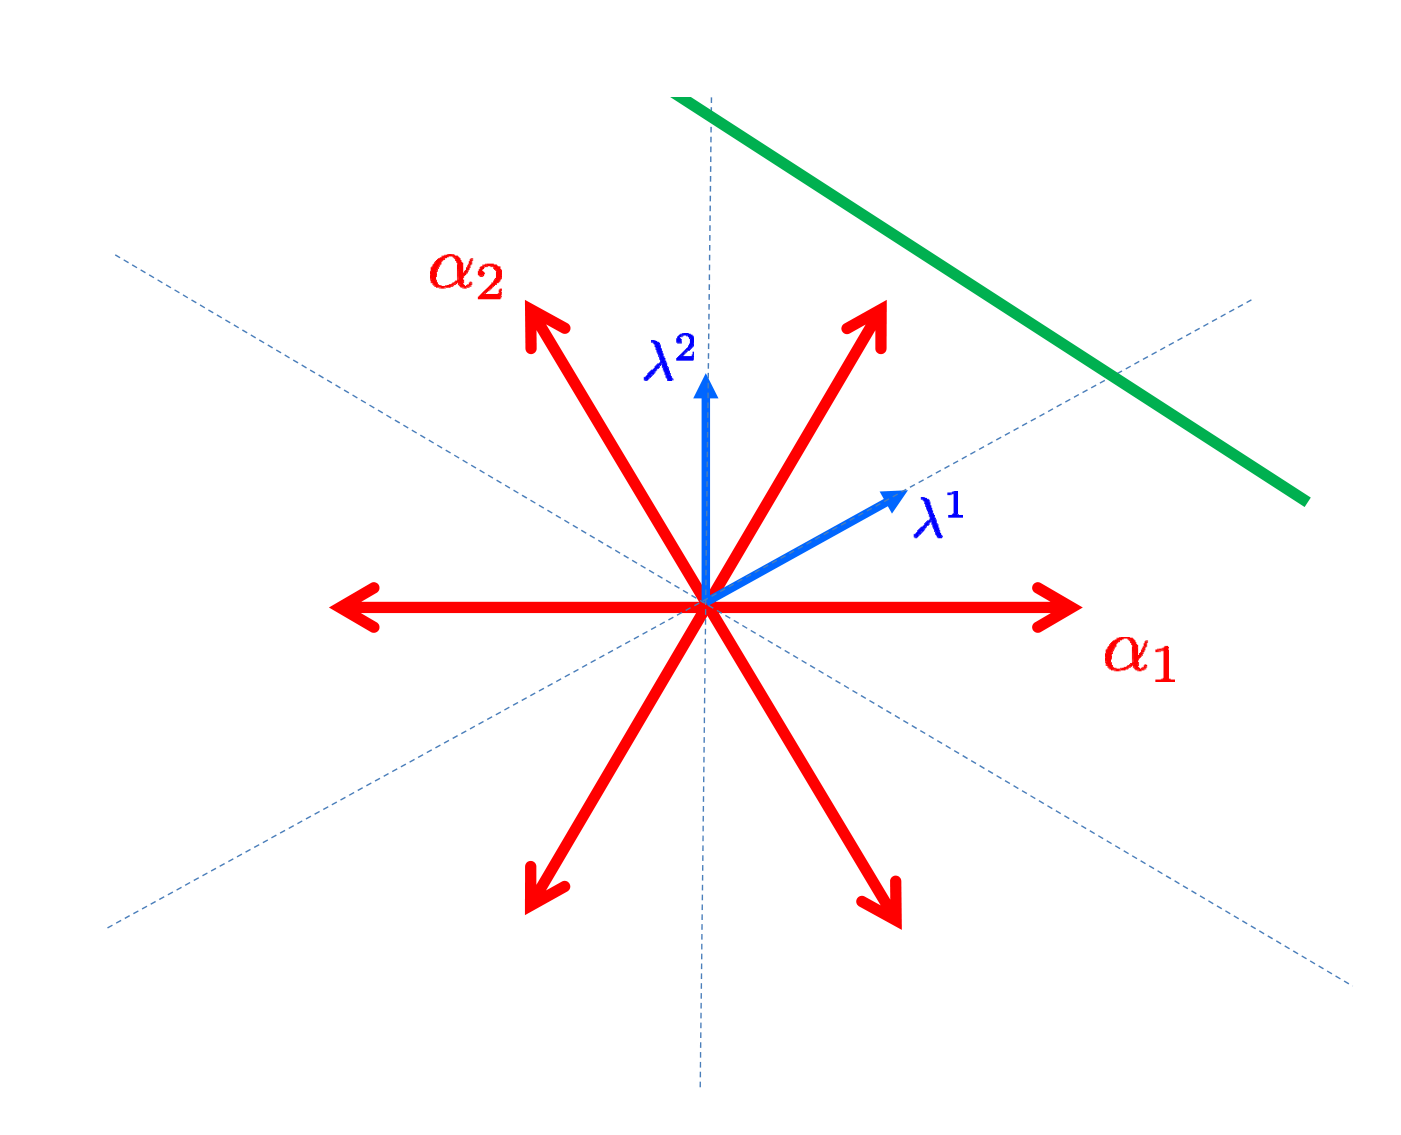
\includegraphics[width=0.62\textwidth]{figures/fig17.png}
  \caption{$SU(3)$ 的根格与权格。图中给出了一组标准的单根 $\alpha_1,\alpha_2$，以及基本权 $\lambda^1,\lambda^2$。基本 Weyl 腔是由这两个权张成的正锥。最高根为 $\theta=\alpha_1+\alpha_2$。粗绿线是某个正整数 $k$ 所对应的直线 $(\lambda,\theta)=k$。仿射 Weyl 腔是区域 $(\lambda,\theta)\le k$，而能级 $k$ 的可积权是权格与基本 Weyl 腔的交集。（原文 Fig.~17，第 129 页）}
  \label{fig:17}
\end{figure}

\subsubsection{可积最高权表示的特征标} % 原文: 4.5.3 Characters of integrable highest weight representations

表示 $V(\lambda)$ 的\emph{特征标}（characters）是
\begin{equation}
  \operatorname{Tr}_{V(\lambda)}q^{L_0}e^{2\pi i\zeta\cdot H_0}
  \tag{4.156}
  \label{eq:4.156}
\end{equation}
其中 $\zeta\in\mathrm{t}^*\otimes\mathbb{C}$，$q=e^{2\pi i\tau}$，$\tau$ 取值于上半平面。
% 原文把 Cartan 子代数记作正体的 $\mathrm{t}$（而非 Fraktur 体的 $\mathfrak{t}$），与 $\mathfrak{g}$、$\widetilde{\mathfrak{g}}$ 的花体形成对照；转写时保持正体。

通过估计各权空间的维数，可以得知这是 $\zeta$ 与 $\tau$ 的整函数。注意：必须把 $L_0$ 计入才能得到有限的表达式。

导出特征标显式的途径有四条：
\begin{enumerate}
  \item 基于 Verma 模构造的代数方法。
  \item 由权重数（weight multiplicities）的递推关系得到的微分方程。
  \item 应用不动点公式与 Borel-Weil-Bott 定理。
  \item 写出相空间路径积分：对在 $G/T$ 上运动的粒子取作用量
  \begin{equation*}
    S\sim\int\langle\lambda,g^{-1}\dot g\rangle-\int dt\,H(g(t)),
  \end{equation*}
  并用驻相法——结果表明驻相法是精确的。对 Weyl 群求和，就是对运动方程的经典解求和。
\end{enumerate}
% 第 4 条把"对 Weyl 群求和"解释为"对经典解求和"，这一步成立的前提是 $G/T$ 上的驻相近似为精确的（等变定位定理）；原文未加证明。

% ===== 原文印刷页 130（PDF p.131）=====

我们只勾勒第 (1) 条途径。Verma 模的特征标是直截了当的，因为它本质上是一个 Fock 空间。抽象地，它可以写成
\begin{equation}
  \frac{e^{\lambda}}{\prod_{\alpha>0}(1-e^{-\alpha})}
  \tag{4.157}
  \label{eq:4.157}
\end{equation}
例如，对 $SU(2)$ 的 $M(2j)$ 我们有
\begin{equation}
  \operatorname{Tr}_{M(2j)}u^{2J_3}=\frac{u^{2j}}{1-u^{-2}}
  \tag{4.158}
  \label{eq:4.158}
\end{equation}
对 $2j\in\mathbb{Z}_{\ge0}$，不可约表示是商 $M(2j)/M(-2j-2)$，因此 $SU(2)$ 的特征标是：
\begin{equation}
\begin{aligned}
  \chi_j(u) &:=\operatorname{Tr}_{V(j)}u^{2J_3}
  =\operatorname{Tr}_{M(2j)}u^{2J_3}-\operatorname{Tr}_{M(-2j-2)}u^{2J_3}\\
  &=\frac{u^{2j}}{(1-u^{-2})}-\frac{u^{-2j-2}}{(1-u^{-2})}
  =\frac{u^{2j+1}-u^{-2j-1}}{u-u^{-1}}
\end{aligned}
  \tag{4.159}
  \label{eq:4.159}
\end{equation}
% 原文 (4.159) 排成单独一行（其编号因此被挤到下一行右侧）；中译本版心较窄，故在第二个等号处折行，编号仍只出现一次。
% [Tutor Note: (4.159) 末式由前式通分得到：两项通分得 $(u^{2j}-u^{-2j-2})/(1-u^{-2})$，再把分子分母同乘 $u$，即得分子 $u^{2j+1}-u^{-2j-1}$、分母 $u-u^{-1}$，可自行验算以免漏掉 $u^{-1}$ 因子。此外 (4.159) 用的是 $u$ 变量，而 (4.168) 之后改用 $y=e^{2\pi iz}$；二者是同一变量 $u=y$，(4.159) 的两项之差正是后文 (4.167) 中 $\Theta_{1,2}-\Theta_{-1,2}$ 的分子，也就是仿射 Weyl 群奇反射 (4.163) 的贡献。]

一般地，对半单的 $\mathfrak{g}$，其不可约表示的特征标是相应 Verma 模特征标的线性组合。利用 Weyl 群的不变性可以证明 Weyl-Kac 特征标公式：
\begin{equation}
  \chi_{\lambda}=\frac{\sum_{w\in W}\epsilon(w)e^{w(\lambda+\rho)-\rho}}{\prod_{\alpha>0}(1-e^{-\alpha})}
  \tag{4.160}
  \label{eq:4.160}
\end{equation}
例如，对 $\widetilde{Lsu(2)}$ 我们有
\begin{equation}
  \operatorname{Tr}_{M(j)}q^{L_0}e^{2\pi i\zeta H_0}
  =\frac{q^{\frac{(j+\frac12)^2-\frac14}{k+2}}e^{2\pi i\zeta(2j)}}
  {(1-e^{-4\pi i\zeta})\prod_{n=1}^{\infty}(1-q^{n})(1-e^{4\pi i\zeta}q^{n})(1-e^{-4\pi i\zeta}q^{n})}
  \tag{4.161}
  \label{eq:4.161}
\end{equation}
分母中的因子分别对应于算符 $J_0^-$、$H_{-n}$、$J_{-n}^+$、$J_{-n}^-$ 作用在最高权向量上的贡献。
% 核对 (4.161) 的 $q$ 指数：$(j+\frac12)^2-\frac14=j(j+1)$，故指数为 $h_j=j(j+1)/(k+2)$，即 $\widehat{su}(2)_k$ 中自旋 $j$ 的最高权态的 $L_0$ 本征值；此处并未减去 $c/24$（$c=3k/(k+2)$），所以 (4.161) 是 Verma 模的迹，与 (4.168) 定义的特征标相差 $q^{-c/24}=q^{-k/(8(k+2))}$。

现在，仿射 Weyl 群一般是 $\Lambda_{weight}\ltimes W$，其中 $W$ 是 $\mathfrak{g}$ 的 Weyl 群。对 $\mathfrak{g}=su(2)$，它就是 $\mathbb{Z}\ltimes\mathbb{Z}_2$，它作用在权上的方式是
\begin{equation}
  j\to j+m(k+2) \qquad m\in\mathbb{Z}
  \tag{4.162}
  \label{eq:4.162}
\end{equation}
对应偶变换，而
\begin{equation}
  j\to -1-j-m(k+2) \qquad m\in\mathbb{Z}
  \tag{4.163}
  \label{eq:4.163}
\end{equation}
对应奇变换。例如：$(J_0^-)^{2j+1}|j\rangle$ 对应于 $m=0$ 的奇 Weyl 反射，而 $(J_{-1}^+)^{k+1-2j}|j\rangle$ 对应于 $m=-1$ 的奇 Weyl 反射，依此类推。

由此我们导出
\begin{equation}
\begin{aligned}
  Tr_{V(j)}\big[q^{L_0}e^{i2\pi z2J_0^3}\big] &= \\
  &= \frac{\sum_m q^{\frac{1}{k+2}\left[(j+\frac12+m(k+2))^2-1/4\right]}
  \left(e^{i4\pi z(j+\frac12+m(k+2))}-e^{-i4\pi z(j+\frac12+m(k+2))}\right)}
  {(e^{2\pi iz}-e^{-2\pi iz})\prod(1-e^{i4\pi z}q^{n})(1-e^{-i4\pi z}q^{n})(1-q^{n})}
\end{aligned}
  \tag{4.164}
  \label{eq:4.164}
\end{equation}
% 原文 (4.164) 左边的 $Tr$ 为斜体，与本页其余公式的正体 $\operatorname{Tr}$ 不一致；照原样转写。又分母的 $\prod$ 未写出指标，应为 $\prod_{n\ge1}$。

% ===== 原文印刷页 131（PDF p.132）=====

对回圈群 $\widetilde{SU(2)}_k$。

现在来了一个漂亮的技巧：对 $j=0,\ k=0$，唯一的幺正不可约表示是平凡表示。因此，分子等于分母。

引入由下式定义的能级 $k$ 的 theta 函数
\begin{equation}
  \Theta_{\mu,k}(z,\tau):=\sum_{n\in\mathbb{Z}}q^{k(n+\mu/(2k))^2}y^{(\mu+2kn)}
  =\sum_{\ell=\mu\operatorname{mod}2k}q^{\ell^2/(4k)}y^{\ell}
  \tag{4.165}
  \label{eq:4.165}
\end{equation}
其中 $y=e^{2\pi iz}$。我们为圆周上粒子引入的 Riemann theta 函数对应于能级 $1/2$。注意：
\begin{equation}
\begin{aligned}
  \Theta_{\mu,k}(\omega,\tau) &= \Theta_{\mu+2ka,k}(\omega,\tau) \qquad a\in\mathbb{Z}\\
  \Theta_{\mu,k}(-\omega,\tau) &= \Theta_{2k-\mu,k}(\omega,\tau)=\Theta_{-\mu,k}(\omega,\tau)
\end{aligned}
  \tag{4.166}
  \label{eq:4.166}
\end{equation}
% (4.165) 第二个等号要求 $\ell\equiv\mu\ (\mathrm{mod}\ 2k)$，故 $\Theta_{\mu,k}$ 只在 $\mu$ 模 $2k$ 的意义下有定义——这正是 (4.166) 第一式的内容。

我们把 $j=0,\ k=0$ 时的分子认作 $\Theta_{1,2}(z,\tau)-\Theta_{-1,2}(z,\tau)$，于是
\begin{equation}
  \Theta_{1,2}(z,\tau)-\Theta_{-1,2}(z,\tau)
  =(e^{2\pi iz}-e^{-2\pi iz})\prod(1-e^{i4\pi z}q^{n})(1-e^{-i4\pi z}q^{n})(1-q^{n})
  =-i\vartheta_1(2z,\tau)
  \tag{4.167}
  \label{eq:4.167}
\end{equation}
接下来是一个概念上重要的步骤。如果我们稍微修改特征标的定义，把它定义为
\begin{equation}
  \chi_j^k(z,\tau):=\operatorname{Tr}_{V(j)}q^{L_0-c/24}e^{2\pi iz(2J_0^3)}
  \tag{4.168}
  \label{eq:4.168}
\end{equation}
特征标就会具有非常漂亮的数学性质。从 Lie 代数理论的角度看这也许显得不自然，但它在物理上有很好的动机：我们减掉的是基态能量。

现在我们可以写出优雅的公式：
\begin{equation}
\begin{aligned}
  \chi_j^k(z,\tau) &:= \operatorname{tr}q^{L_0-c/24}e^{2\pi iz(2J_0^3)}\\
  &= \frac{\Theta_{2j+1,k+2}(z,\tau)-\Theta_{-2j-1,k+2}(z,\tau)}{\Theta_{1,2}(z,\tau)-\Theta_{-1,2}(z,\tau)}\\
  &= q^{(\ell+1)^2/(4(k+2))-1/8}\chi_j(y)+\cdots
\end{aligned}
  \tag{4.169}
  \label{eq:4.169}
\end{equation}
其中 $0\le j\le k/2$，且 $j$ 取半整数。
% [Tutor Note: (4.169) 有三处易错：(i) 第二行分母用 $\Theta_{1,2}-\Theta_{-1,2}$（能级 2、指标 $\pm1$），分子用能级 $k+2$、指标 $\pm(2j+1)$；(ii) 第三行末尾的 $\chi_j(y)$ 是 $SU(2)$ 的**群**特征标（即 (4.159) 的 $\chi_j(u)$ 取 $u=y=e^{2\pi iz}$），与左边的**仿射**特征标 $\chi_j^k$ 同符号但含义不同；(iii) 第三行 $q$ 的指数应为 $h_j-c/24=j(j+1)/(k+2)-k/(8(k+2))$，而原文写的是 $(\ell+1)^2/(4(k+2))-1/8$，其中 $-1/8$ 只是 $-k/(8(k+2))$ 在 $k\to\infty$ 时的极限，故第三行应读作大 $k$ 领头渐近项，一般 $k$ 下需替换。]

\subsubsection{模性质} % 原文: 4.5.4 Modular properties

特征标满足许多漂亮的数学性质。它们给出 \emph{Jacobi 形式}（Jacobi forms）的例子。当特殊化到 $\zeta=0$ 时，它们在 $PSL(2,\mathbb{Z})$ 下构成一个由\emph{模形式}（modular forms）组成的向量。

回忆 $SL(2,\mathbb{Z})$ 是 $SL(2,\mathbb{R})$ 中矩阵元为整数的子群。它由 $S$、$T$ 生成，二者分别在附录 C 的公式 (C.2) 与 (C.3) 中定义。

{\small\itshape ［原文标记：与附录 D 中的公式重复。］}
% [原文待办标记，原文 p.131 页边；作者用 \ensuremath{\clubsuit} 标出的旁注，提示此处与附录 D 的公式重复]

$SL(2,\mathbb{Z})$ 通过
\begin{equation}
  (\tau,z)\to\Big(\frac{a\tau+b}{c\tau+d},\frac{z}{c\tau+d}\Big)
  \tag{4.170}
  \label{eq:4.170}
\end{equation}
作用在 $(\tau,z)$ 上。

% ===== 原文印刷页 132（PDF p.133）=====

注意它在 $\tau$ 上的作用经过 $PSL(2,\mathbb{Z}):=SL(2,\mathbb{Z})/\langle-1\rangle$ 分解。注意 $T:\tau\to\tau+1$，$S:\tau\to-1/\tau$。

利用 Poisson 求和公式，可以验证能级 $k$ 的 theta 函数在 $SL(2,\mathbb{Z})$ 的生成元下的变换规律：
\begin{equation}
  \Theta_{\mu,k}(\omega,\tau+1)=e^{2\pi i\frac{\mu^2}{4k}}\Theta_{\mu,k}(\omega,\tau)
  \tag{4.171}
  \label{eq:4.171}
\end{equation}
\begin{equation}
  \Theta_{\mu,k}(-\omega/\tau,-1/\tau)=(-i\tau)^{1/2}e^{2\pi ik\omega^2/\tau}
  \sum_{\nu=0}^{2k-1}\frac{1}{\sqrt{2k}}e^{2\pi i\frac{\mu\nu}{2k}}\Theta_{\nu,k}(\omega,\tau)
  \tag{4.172}
  \label{eq:4.172}
\end{equation}
由 \eqref{eq:4.172} 可以推出
\begin{equation}
  (\Theta_{1,2}-\Theta_{-1,2})(-z/\tau,-1/\tau)
  =i(-i\tau)^{1/2}e^{4\pi iz^2/\tau}(\Theta_{1,2}-\Theta_{-1,2})(z,\tau)
  \tag{4.173}
  \label{eq:4.173}
\end{equation}
再做一点简短的计算便得到：
\begin{equation}
  \chi_j^{su(2)}(-1/\tau,-z/\tau)=e^{2\pi ikz^2/\tau}
  \sum_{j'=0}^{k/2}S_{jj'}\chi_{j'}^{su(2)}(\tau,z)
  \tag{4.174}
  \label{eq:4.174}
\end{equation}
其中
\begin{equation}
  S_{jj'}=\sqrt{\frac{2}{k+2}}\sin\frac{\pi(2j+1)(2j'+1)}{k+2}.
  \tag{4.175}
  \label{eq:4.175}
\end{equation}
$T$ 的作用容易算出为：
\begin{equation}
  \chi_j^k(\tau+1,z)
  =e^{2\pi i\left(\frac{(\ell+1)^2}{4(k+2)}-\frac18\right)}\chi_j^k(\tau,z)
  =e^{2\pi i\frac{2\ell(\ell+2)-k}{8(k+2)}}\chi_j^k(\tau,z)
  \tag{4.176}
  \label{eq:4.176}
\end{equation}
其中 $\ell=2j$。这两个变换生成模群 $SL(2,\mathbb{Z})$ 的一个幺正表示。
% [Tutor Note: (4.175) 是 $\widehat{su}(2)_k$ 的模 $S$ 矩阵；核对归一化最省事的办法是用 $S^2=\mathbf{1}$ 的实形式（$S$ 对称且 $S^2$ 给出电荷共轭 $\mu\to-\mu$），以及 $j\to k/2-j$ 时 $\sin$ 的对称性。注意 (4.174) 左边变量顺序是 $(-1/\tau,-z/\tau)$，而 (4.168) 中 $z$ 出现在 $e^{2\pi iz(2J_0^3)}$ 里，故必须配合 (4.176) 与 (4.172) 才能得到不含前因子 $e^{2\pi ikz^2/\tau}$ 的"纯"矩阵元；漏掉前因子是常见错误。]

\textbf{注记}

\begin{enumerate}
  \item 一般地，特征标由 Weyl-Kac 特征标公式给出。正如 Weyl 特征标公式可以写成
  \begin{equation}
    \frac{\sum_{w\in W}e^{w(\lambda+\rho)-\rho}}{\sum_{w\in W}e^{w(\rho)-\rho}}
    \tag{4.177}
    \label{eq:4.177}
  \end{equation}
  Weyl-Kac 特征标公式也可以写成完全同样的形式，只需把对 Weyl 群的求和换成对仿射 Weyl 群的求和，并把 $\lambda$、$\rho$ 换成相应的仿射权。我们在公式 (??) 中认出了对仿射 Weyl 群求和的结构：theta 函数来自对 $\mathbb{Z}$ 的求和，而 theta 函数之差来自 $SU(2)$ 的 Weyl 群中那个非平凡的反射。
% [原文待办标记，原文 p.132；"equation (??)" 是作者未填写的交叉引用，从上下文看应指 (4.169)（或与之等价的 (4.164)），此处照原样保留问号]
  \item 一般地可以取 $\lambda=0$，得到分母恒等式：
  \begin{equation}
    \sum_{w\in W}\epsilon(w)e^{w(\rho)}=\prod_{\alpha>0}\big(e^{\frac12\alpha}-e^{-\frac12\alpha}\big)
    \tag{4.178}
    \label{eq:4.178}
  \end{equation}
\end{enumerate}

% ===== 原文印刷页 133（PDF p.134）=====

\begin{enumerate}[start=3]
  \item 在广义 Kac-Moody 代数上，\eqref{eq:4.178} 有许多很有意思的推广。{\small\itshape ［原文标记：此处需要补文献！］}
% [原文待办标记，原文 p.133；原文作 "[NEED CITATIONS HERE!]"]
  \item 事实表明，$G_k$ 的表示论与相应量子群在 $q$ 取适当单位根时的表示论密切相关：
  \begin{equation}
    q=\exp\Big(\frac{2\pi i}{k+h}\Big)
    \tag{4.179}
    \label{eq:4.179}
  \end{equation}
  详见 Fuchs 的书。
  \item 上述故事可以推广到更广的一类二维共形场论，即所谓"有理共形场论"（rational conformal field theories）。
\end{enumerate}

\medskip\noindent\textbf{练习}\quad 仔细解释为什么 $j=k=0$ 的不可约表示是平凡表示。

\noindent 证明 $M(j=0,k=0)/S(j=0,k=0)$ 是一维的。

\medskip\noindent\textbf{练习}\quad 求出 $\widetilde{su(3)}$ 在能级 $k$ 的可积表示，并说明它们在权格上如何分布。

\subsection{WZW 的 Hilbert 空间与单圈配分函数} % 原文: 4.6 The Hilbert Space Of WZW And The One-Loop Partition Function

% 本片段无 \section 级标题（4.6 为 \subsection），故按规范不插入「本节重点」；该小节要点备忘：
% (i) $\mathcal{H}=\oplus_{0\le\lambda\cdot\theta\le k}\overline{V_\lambda}\otimes V_\lambda$ 是 Peter-Weyl 定理的精确类比，每个幺正不可约表示恰好出现一次；
% (ii) 单圈配分函数等于以 $\tau=\theta+i\beta$ 为模参数的平坦环面上的路径积分，$H=L_0+\bar{L}_0-c/12$、$P=L_0-\bar{L}_0$；
% (iii) 微分同胚不变性 + 共形反常下 Weyl 标度贡献为零 $\Rightarrow$ $Z$ 模不变，由 $\chi_\lambda$ 的幺正模表示保证；
% (iv) 存在非对角模不变组合 $\sum N_{j\bar j}\chi_j\overline{\chi_{\bar j}}$（$N$ 非单位矩阵倍数）。

Hilbert 空间与单圈配分函数。

注：大 $k$ 极限：粒子在群 $G$ 上运动。$L^2(G)$ 分解的截断。环面上的共形块。$S$ 矩阵与 $T$ 矩阵。
% 这几行是作者的写作提纲（"Note: ..."），并非完整句子，译文按原样逐句译出、未作展开；它预告了本节的三条主线：大 $k$ 的粒子图像、$L^2(G)$ 分解被截断到 $(\lambda,\theta)\le k$ 的有限多项、以及环面上共形块的 $S$、$T$ 矩阵。

对紧群 $G$，Hilbert 空间具有漂亮的结构。事实证明，Hilbert 空间关于量子 $\widetilde{LG}_L\times\widetilde{LG}_R$ 对称性的分解，把每一个幺正不可约表示都恰好编码一次。因此，它是紧群 Peter-Weyl 定理的完美类比。

我们有
\begin{equation}
  \mathcal{H}=\oplus_{0\le\lambda\cdot\theta\le k}\overline{V_{\lambda}}\otimes V_{\lambda}
  \tag{4.180}
  \label{eq:4.180}
\end{equation}
其中
\begin{equation}
  0\le\lambda\cdot\theta\le k
  \tag{4.181}
  \label{eq:4.181}
\end{equation}
而 $\theta$ 是 $\mathfrak{g}$ 的最高根。对 $SU(2)$ 能级 $k$ 的模型，我们特别有：

% ===== 原文印刷页 134（PDF p.135）=====

\begin{equation}
  \mathcal{H}=\oplus_{0\le j\le k/2}\overline{V_j}\otimes V_j
  \tag{4.182}
  \label{eq:4.182}
\end{equation}
特征标的模性质现在得到了漂亮的解释。考虑配分函数：
\begin{equation}
  Z=\operatorname{Tr}_{\mathcal{H}}e^{-2\pi\beta H+2\pi i\theta P}
  =\operatorname{Tr}_{\mathcal{H}}q^{L_0-c/24}\bar{q}^{\bar{L}_0-c/24}
  \tag{4.183}
  \label{eq:4.183}
\end{equation}
其中
\begin{equation}
  H=L_0+\bar{L}_0-c/12
  \tag{4.184}
  \label{eq:4.184}
\end{equation}
\begin{equation}
  P=L_0-\bar{L}_0
  \tag{4.185}
  \label{eq:4.185}
\end{equation}
而
\begin{equation}
  \tau=\theta+i\beta
  \tag{4.186}
  \label{eq:4.186}
\end{equation}
于是
\begin{equation}
  Z=\sum_{\lambda}\overline{\chi_{\lambda}(\tau,0)}\chi_{\lambda}(\tau,0)
  \tag{4.187}
  \label{eq:4.187}
\end{equation}
{\small\itshape ［原文标记：这里真的需要补上与平坦规范场的耦合！！！］}
% [原文待办标记，原文 p.134 页边；作者用 \ensuremath{\clubsuit} 标出的旁注 "REALLY NEED TO ADD COUPLING TO FLAT GAUGE FIELDS HERE!!!"，提示应在 (4.187) 处加入与平坦背景规范场的耦合]

% [Tutor Note: 原 PDF 第 134 页的 Figure 18 为空白占位框，图形内容在原稿中缺失，仅存图注；此处按原图注翻译并保留图号，以免后文图号错位。]
\begin{figure}[htbp]
  \centering
  \MissingFigureNote
  \caption{取迹在 $z=\sigma+it$ 平面上所诱导的等同（identifications）。我们先沿欧氏时间传播 $\beta$，然后在等同状态之前，沿 $\sigma$ 方向作一个 $2\pi\theta$ 的平移扭转。（原文 Fig.~18，第 134 页）}
  \label{fig:18}
\end{figure}
% [排版说明：原 PDF 中 Fig.~18 的图形本身缺失，页面上只余图注与留白，figures/fig18.png 为对应的空白裁片，按原样插入以保留编号与位置]

配分函数 \eqref{eq:4.183} 可以解释为平坦环面上的路径积分，该环面的模参数为 $\tau$，如图 18 所示。我们将在第 2.2.12 节看到，$\tau$ 上的模变换等价于环面上非平凡微分同胚的作用。

另一方面，配分函数必须是微分同胚不变的。Weyl 标度对配分函数的影响为零，这是由于共形反常，并且背景度规是平坦的。因此，配分函数必须是模不变的。这一点得以实现，是因为 $\chi_{\lambda}$ 按模群的幺正表示变换。

\textbf{注记}：存在不同的模不变特征标组合。也就是说，可以找到非负整数 $N_{j,\bar{j}}$，它们不正比于单位矩阵，使得
\begin{equation}
  \sum_{j,\bar{j}}N_{j\bar{j}}\chi_{j}\overline{\chi_{\bar{j}}}
  \tag{4.188}
  \label{eq:4.188}
\end{equation}
% (4.188) 中的 $\bar{j}$ 表示右移（反全纯）侧的指标，与左移的 $j$ 独立取值，二者各自遍历 $0\le j\le k/2$，不可混为同一个指标；$N_{j\bar j}$ 取单位矩阵即退化为对角组合 (4.187)。

% =====================================================================
%  c16 —— 原文印刷页 135–141（PDF 第 136–142 页）
%  含：4.7 Primary Fields（4.7.1、4.7.2）与 4.8 Tensor Product Of Highest
%  Weight Representations 的开头部分；插图 Fig. 19。
% =====================================================================

是模不变的。它们对应着其他的理论。

对 $G=SU(2)$，模不变量具有 ADE 分类，见 Capelli、Itzkyson、Zuber 的一篇漂亮论文。

对 $G=SU(3)$，分类由 Terry Gannon 完成（hep-th/9212060、hep-th/9404185）。论文 hep-th/9604104："Comments on the Links between su(3) Modular Invariants, Simple Factors in the Jacobian of Fermat Curves, and Rational Triangular Billiards"（作者 M. Bauer、A. Coste、C. Itzykson、P. Ruelle）揭示了与数学各个分支之间引人入胜的联系。

对更高秩的群，完整的分类尚属未知（？）

{\small\itshape ［原文标记：数学家对朴素的对角模不变量有些意见。这一点我是从 A. Neitzke 那里得知的。（2019 年 5 月 8 日）］}
% [原文待办标记，原文 p.135；原文以两行星号分隔线上下框住这段全大写文字，所标记的是「朴素的对角模不变量」这一选择在数学上的问题]

\subsection{主场} % 原文: 4.7 Primary Fields

态–算符对应：主场顶点算符

全纯因子化：手征顶点算符。

COMMENT：顶点算符代数（vertex operator algebras）与纯代数进路。（Borcherds、FLM、Lepowsky–Huang 等）

OPE–融合规则：F 矩阵。自洽性：五边形公理。

惊喜！$S$ 对角化融合规则！Verlinde 公式。

\subsubsection{半单代数} % 原文: 4.7.1 Semisimple Algebras

评注：关于一般半单代数的"Verlinde 公式"。给出有限群环的例子。练习：有限群论中的融合规则与 Verlinde 公式。

一般而言，事情就到此为止。不过，当该代数 $(\mathcal{C},\theta)$ 是半单的时候，还可以多说一点。

半单性最为有用的刻画如下。结构常数\footnote{结构常数 $N_{\mu\nu}^{\ \ \lambda}$ 不必是整数。但在许多有趣的例子中，代数存在一组基，使得它们在事实上取整数值。}
\begin{equation}
  \phi_\mu\phi_\nu=N_{\mu\nu}^{\ \ \lambda}\phi_\lambda
  \tag{4.189}
  \label{eq:4.189}
\end{equation}
这些结构常数通过左正则表示（left-regular representation）$L(\phi_\mu)$ 定义出一族矩阵，其矩阵元为 $N_{\mu\nu}^{\ \ \lambda}$。由于 $\mathcal{C}$ 可交换，这些矩阵两两交换。于是：

\textbf{定义}：$\mathcal{C}$ 是半单的，当且仅当矩阵 $L(\phi_\mu)$ 可同时对角化。

于是，在半单情形我们可以找到矩阵 $S$，使得
\begin{equation}
  N_{\mu\nu}^{\ \ \lambda}=\sum_x S_\nu^{\ x}\Lambda_x^{(\mu)}(S^{-1})_x^{\ \lambda}
  \tag{4.190}
  \label{eq:4.190}
\end{equation}

其中 $\Lambda_x^{(\mu)}$ 是 $L(\phi_\mu)$ 的各不相同的本征值。

现在我们选取一组基，使指标 $\mu$ 取遍 $\mu=0,\dots,n$，并取 $\phi_0=1_{\mathcal{C}}$，即乘法单位元。把 $\mu=0$ 代入 \eqref{eq:4.190} 得到的只是一个平凡的恒等式；但若代入 $\nu=0$，并利用 $N_{\mu\nu}^{\ \ \lambda}=N_{\nu\mu}^{\ \ \lambda}$（从而 $N_{\mu 0}^{\ \ \lambda}=\delta_\mu^{\ \ \lambda}$），我们便看出 $S_0^{\ x}\Lambda_x^{(\mu)}=S_\mu^{\ x}$，因为这里用到的正是 $S^{-1}$ 的矩阵逆（即 $S$ 本身）。故
\begin{equation}
  S_0^{\ x}\Lambda_x^{(\mu)}=S_\mu^{\ x}\qquad\qquad\text{no sum on }x
  \tag{4.191}
  \label{eq:4.191}
\end{equation}

把它代回 \eqref{eq:4.190}，我们得到
\begin{equation}
  N_{\mu\nu}^{\ \ \lambda}=\sum_x\frac{S_\nu^{\ x}S_\mu^{\ x}(S^{-1})_x^{\ \lambda}}{S_0^{\ x}}
  \tag{4.192}
  \label{eq:4.192}
\end{equation}
% [Tutor Note: 原稿把矩阵指标排成「错位」形式：$N_{\mu\nu}^{\ \ \lambda}$、$S_\nu^{\ x}$、$(S^{-1})_x^{\ \lambda}$ 里最后一个指标特意错开一格，表示它与 $\mu,\nu$ 不同类（$\mu,\nu$ 是代数乘积的下指标，另一个是基指标）。转写时若丢掉 \ 留出的空位，就会误以为 $x$ 是紧贴 $S_\nu$ 的第一上标，从而把 (4.192) 的分子读错。(4.190) 的矩阵含义是 $L(\phi_\mu)=S\Lambda^{(\mu)}S^{-1}$（矩阵元为 $(L(\phi_\mu))_\nu^{\ \lambda}=N_{\mu\nu}^{\ \ \lambda}$）；核对时把它与 (4.190) 逐项对照，即可确认 $S_\nu^{\ x}$ 与 $(S^{-1})_x^{\ \lambda}$ 的配对，也能看出 (4.191) 为何必须标注「no sum on $x$」：该式对每个 $x$ 单独成立，$x$ 是标记本征值的标号而非求和指标]

注意 $\theta(\phi_\mu\phi_\nu\phi_\lambda)=N_{\mu\nu}^{\ \ \lambda'}Q_{\lambda'\lambda}:=N_{\mu\nu\lambda}$ 关于 $\mu,\nu,\lambda$ 全对称。假设我们进一步把注意力限制在满足 $\theta(\phi_\mu)=\delta_{\mu,0}$ 的基 $\{\phi_\mu\}$ 上。那么对 \eqref{eq:4.189} 取迹便知 $Q_{\mu\nu}=N_{\mu\nu}^{\ \ 0}$，而 \eqref{eq:4.192} 随后给出
\begin{equation}
  Q_{\mu\nu}=\sum_x S_\nu^{\ x}S_\mu^{\ x}\frac{(S^{-1})_x^{\ 0}}{S_0^{\ x}}
  \tag{4.193}
  \label{eq:4.193}
\end{equation}
从而
\begin{equation}
  N_{\mu\nu\lambda}=\sum_x S_\mu^{\ x}S_\nu^{\ x}S_\lambda^{\ x}\frac{(S^{-1})_x^{\ 0}}{(S_0^{\ x})^2}
  \tag{4.194}
  \label{eq:4.194}
\end{equation}

若作线性组合
\begin{equation}
  \epsilon_x=\sum_\mu S_0^{\ x}(S^{-1})_x^{\ \mu}\phi_\mu
  \tag{4.195}
  \label{eq:4.195}
\end{equation}
则 $\epsilon_x$ 构成一组基本幂等元（basic idempotents），即
\begin{equation}
  \begin{gathered}
    \mathcal{C}=\oplus_x\mathbb{C}\epsilon_x\\
    \epsilon_x\epsilon_y=\delta_{x,y}\epsilon_y
  \end{gathered}
  \tag{4.196}
  \label{eq:4.196}
\end{equation}
% [Tutor Note: 「$\epsilon_x$ 给出 $\mathcal{C}$ 的直和分解」等价于有限维可交换半单代数（且带非退化对称双线性型，即本文的 $\theta$）的结构定理——Artin–Wedderburn 定理的交换情形，作者此处写 "that is" 直接给出，未作证明。被略去的一步是：$L(\phi_\mu)$ 可同时对角化 $\Rightarrow$ 存在公共本征向量基 $\Rightarrow$ Lagrange 插值可构造出两两正交的幂等元；反过来由幂等元存在则 $L(\phi_\mu)$ 在基 $\epsilon_x$ 下对角。这一步与 $\theta$ 无关，纯属线性代数，可查任意一本代数教材的「半单代数」一节]

此外，若取自然归一化 $\theta(\phi_\mu)=\delta_{\mu,0}$，则
\begin{equation}
  \theta_x:=\theta_{\mathcal{C}}(\epsilon_x)=S_0^{\ x}(S^{-1})_x^{\ 0}
  \tag{4.197}
  \label{eq:4.197}
\end{equation}

这里 $\theta_i$ 是一些非零复数。无序集合 $\{\theta_x\}$ 是有限维可交换半单 Frobenius 代数的唯一不变量。
% [Tutor Note: 原文此处写 $\theta_i$，而前后文一律用 $\{\theta_x\}$（$x$ 标记幂等元、$\mu,\nu,\lambda$ 标记基元素），从 (4.197) 的指标也可看出应为 $\theta_x$。译文照原文转写 $\theta_i$ 未改，但引用 (4.197)、(4.199)、(4.200) 时应按 $\theta_x$ 理解]

% [原文标记：此处有两行纯星号分隔线（原稿的分段记号，无文字），原文 p.136]
{\small\itshape ［原文标记：以下部分材料应当移到"拓扑场论"一章——二维 TFT 的例子：］}
% [原文待办标记，原文 p.136；作者希望把随后关于二维 TFT 的整段讨论挪到拓扑场论一章]

注意在此情形，特征元（characteristic element）简单地就是
\begin{equation}
  H=\sum_x\frac{1}{\theta_x}\epsilon_x
  \tag{4.198}
  \label{eq:4.198}
\end{equation}
从而在亏格为 $g\ge0$ 的曲面上的真空振幅为
\begin{equation}
  Z_g=\sum_x\theta_x^{1-g}
  \tag{4.199}
  \label{eq:4.199}
\end{equation}

\textbf{评注}：

\begin{enumerate}
  \item 若考虑对所有亏格的求和，则该求和只在 $|\theta_x|>1$ 时收敛（在单位圆上为条件收敛），此时它等于
  \begin{equation}
    Z_{\mathrm{string}}=\sum_x\frac{\theta_x}{1-\theta_x^{-1}}
    \tag{4.200}
    \label{eq:4.200}
  \end{equation}

  \item 注意至此还没有任何东西固定矩阵 $S$ 的整体归一化。在某些情形 $S$ 是幺正的，从而 $(S^{-1})_x^{\ 0}=(S_0^{\ x})^*$。此外，若矩阵元 $S_0^{\ x}$ 可以取为实数，则 \eqref{eq:4.194} 有一个漂亮的简化：
  \begin{equation}
    N_{\mu\nu\lambda}=\sum_x\frac{S_\mu^{\ x}S_\nu^{\ x}S_\lambda^{\ x}}{S_0^{\ x}}
    \tag{4.201}
    \label{eq:4.201}
  \end{equation}
\end{enumerate}

这正是 Verlinde 公式通常的表述形式。

\textbf{练习}\quad 证明本征值 $\Lambda_x^{(\rho)}$ 满足代数关系
\begin{equation}
  \Lambda_x^{(\mu)}\Lambda_x^{(\nu)}=\sum_\lambda N_{\mu\nu}^{\ \ \lambda}\Lambda_x^{(\lambda)}
  \tag{4.202}
  \label{eq:4.202}
\end{equation}

\textbf{练习}\quad 场论中一个自然的问题是：一个理论的真空振幅是否完全决定了该理论中的一切振幅。请就半单二维 TFT 的情形研究这一问题。

% [原文标记：此处有两行纯星号分隔线（原稿的分段记号，无文字），原文 p.137]

\subsubsection{半单融合规则的一个例子：有限群论} % 原文: 4.7.2 An Example Of Semisimple Fusion Rules: Finite Group Theory

设 $G$ 为有限群。复值函数空间 $\mathbb{C}[G]$ 在逐点乘法给出的显然乘积
\begin{equation}
  f_1\cdot f_2(g):=f_1(g)f_2(g)
  \tag{4.203}
  \label{eq:4.203}
\end{equation}
之下是一个 $C^*$ 代数（见下文）。

令 $\mathcal{C}$ 为类函数（class functions）的子空间，即满足
\begin{equation}
  f(hgh^{-1})=f(g)\qquad\forall g,h\in G
  \tag{4.204}
  \label{eq:4.204}
\end{equation}
的函数全体。这是 $G$ 的（有限个）共轭类所成集合上的函数空间。

$\mathcal{C}$ 有两组自然的函数基。其中一组使 $\mathcal{C}$ 显然以自然的方式成为一个 Frobenius 代数，另一组则使这个 Frobenius 代数的半单性一目了然。

类函数空间的第一组自然基由各不相同的不可约表示的特征标 $\chi_\mu$ 给出，$\mu$ 标记 $G$ 的各不相同的不可约表示。

在逐点乘法下
\begin{equation}
  \chi_\mu\chi_\nu=\sum_\lambda N_{\mu\nu}^{\ \ \lambda}\chi_\lambda
  \tag{4.205}
  \label{eq:4.205}
\end{equation}
其中 $N_{\mu\nu}^{\ \ \lambda}$ 是融合系数（fusion coefficients）（它们也被称为"Littlewood–Richardson 系数"）。它们由 Clebsch–Gordon 级数
\begin{equation}
  T^\mu\otimes T^\nu=\oplus_\lambda N_{\mu\nu}^{\ \ \lambda}T^\lambda
  \tag{4.206}
  \label{eq:4.206}
\end{equation}
确定，并且是非负整数。自然的迹为
\begin{equation}
  \theta(\chi_\mu)=\delta_{\mu,0}
  \tag{4.207}
  \label{eq:4.207}
\end{equation}
其中 $\chi_0=1$ 对应平凡表示。由于对每个表示 $\mu$ 都存在表示 $\mu^*$ 使得 $\chi_\mu\chi_{\mu^*}=\chi_0+\cdots$，我们断定 $\langle f,g\rangle=\theta(fg)$ 非退化，从而 $\mathcal{C}$ 确实是一个 Frobenius 代数。

类函数的另一组自然基是共轭类上的 delta 函数：
\begin{equation}
  \begin{aligned}
    \delta_C(g)&=1&&g\in C\\
    &=0&&g\notin C
  \end{aligned}
  \tag{4.208}
  \label{eq:4.208}
\end{equation}
其中 $C$ 是一个共轭类。注意在这组基下，逐点乘法是对角的。于是 $\mathcal{C}$ 的半单性便是显然的。

我们当然可以把一组基按另一组展开：
\begin{equation}
  \chi_\mu=\sum_i\chi_\mu(C_i)\delta_{C_i}
  \tag{4.209}
  \label{eq:4.209}
\end{equation}

现在回忆群表示论中的一个标准结果：不可约表示的特征标所满足的正交关系
\begin{equation}
  \frac{1}{|G|}\sum_g\chi_\mu(g)\chi_\nu(g^{-1})=\delta_{\mu,\nu}
  \tag{4.210}
  \label{eq:4.210}
\end{equation}

由于 $G$ 有限，不失一般性（WLOG）可假定表示 $T^\mu$ 是幺正的。因此矩阵
\begin{equation}
  S_{i\mu}=\sqrt{\frac{m_i}{|G|}}\chi_\mu(C_i)
  \tag{4.211}
  \label{eq:4.211}
\end{equation}
（其中 $m_i$ 是类 $|C_i|$ 的阶）是幺正矩阵。

现在我们有
\begin{equation}
  \chi_\mu=\sum_i\sqrt{\frac{|G|}{m_i}}S_{i\mu}\delta_{C_i}
  \tag{4.212}
  \label{eq:4.212}
\end{equation}
因此，由于乘法在基 $\delta_{C_i}$ 下是对角的，$S_{i\mu}$ 就是在特征标基下对角化融合规则的那个矩阵。
% [Tutor Note: (4.211) 的幺正性来自 (4.210)：把 $\sum_g$ 按共轭类分组后，$\sum_g\chi_\mu(g)\chi_\nu(g^{-1})=\sum_i m_i\chi_\mu(C_i)\chi_\nu(C_i)$（用了 $\chi_\nu(g^{-1})=\chi_\nu(g)^*$，这正是「$T^\mu$ 可取幺正」的作用），代入 (4.211) 即得 $\sum_i S_{i\mu}S_{i\nu}^*=\delta_{\mu\nu}$。另需注意原文 "where $m_i$ is the order of the class $|C_i|$" 的措辞含糊：$m_i$ 就是共轭类 $C_i$ 的元素个数，即 $m_i=|C_i|$，与记号 $|C_i|$ 指同一个量，(4.214) 中的 $|G|$ 则是群的阶，勿混]

现在，利用 \eqref{eq:4.197} 我们算得
\begin{equation}
  \theta_x=|S_{0x}|^2=\frac{(\dim V_x)^2}{|G|}
  \tag{4.213}
  \label{eq:4.213}
\end{equation}

{\small\itshape ［原文标记：把这一段移到"拓扑场论——二维例子"一章。］}
% [原文待办标记，原文 p.139；该行上、下各有一行星号分隔线]

从而亏格为 $g$ 的紧 Riemann 面上的配分函数为
\begin{equation}
  Z_g=|G|^{1-g}\sum_x\frac{1}{(\dim V_x)^{2g-2}}
  \tag{4.214}
  \label{eq:4.214}
\end{equation}
其中求和遍历 $G$ 的全部不可约表示。第一个因子相对无趣（它可以被吸收进弦耦合常数的标度之中），但第二个因子很有趣。

\emph{\eqref{eq:4.214} 中的求和究竟在计数什么样的几何对象？}

我们将在随后几讲中回答这个问题。

% [原文标记：此处有两行纯星号分隔线（原稿的分段记号，无文字），原文 p.140]

\textbf{练习}
\begin{enumerate}[label=\alph*.)]
  \item 证明带卷积乘积的群代数 $\mathbb{C}[G]$ 的中心就是 $\mathcal{C}$，即类函数空间。
  \item 证明矩阵 $S_{i\mu}$ 是 $\mathcal{C}$ 上这两种乘积结构之间的一种 Fourier 变换。注意各不可约表示的特征标基 $\chi_\mu$ 对角化卷积乘积：
  \begin{equation}
    \chi_\mu*\chi_\nu=\frac{\delta_{\mu\nu}}{n_\nu}\chi_\nu
    \tag{4.215}
    \label{eq:4.215}
  \end{equation}
  \item 证明这个 Frobenius 代数的诸不变量 $\theta_x$ 由
  \begin{equation}
    \theta(\epsilon_\mu)=\frac{(\dim V_\mu)^2}{|G|}
    \tag{4.216}
    \label{eq:4.216}
  \end{equation}
  给出。
\end{enumerate}
% [Tutor Note: 原文用斜体 $C[G]$ 表示复群代数（即 $\mathbb{C}[G]$），与类函数子空间的花体 $\mathcal{C}$ 只是同一字母的两种字体，含义完全不同；译文以 $\mathbb{C}[G]$ 与 $\mathcal{C}$ 区分，避免混淆。又，原文本节把 $S_{i\mu}$ 的下标排成「类在前、不可约表示在后」，而 (4.197) 中的 $S$ 是「指标 $x$ 在前」；两处 $S$ 相差转置与相位约定（(4.213) 只用到 $|S_{0x}|^2$，故不受影响），逐式核对时需留意]

\begin{figure}[htbp]
  \centering
  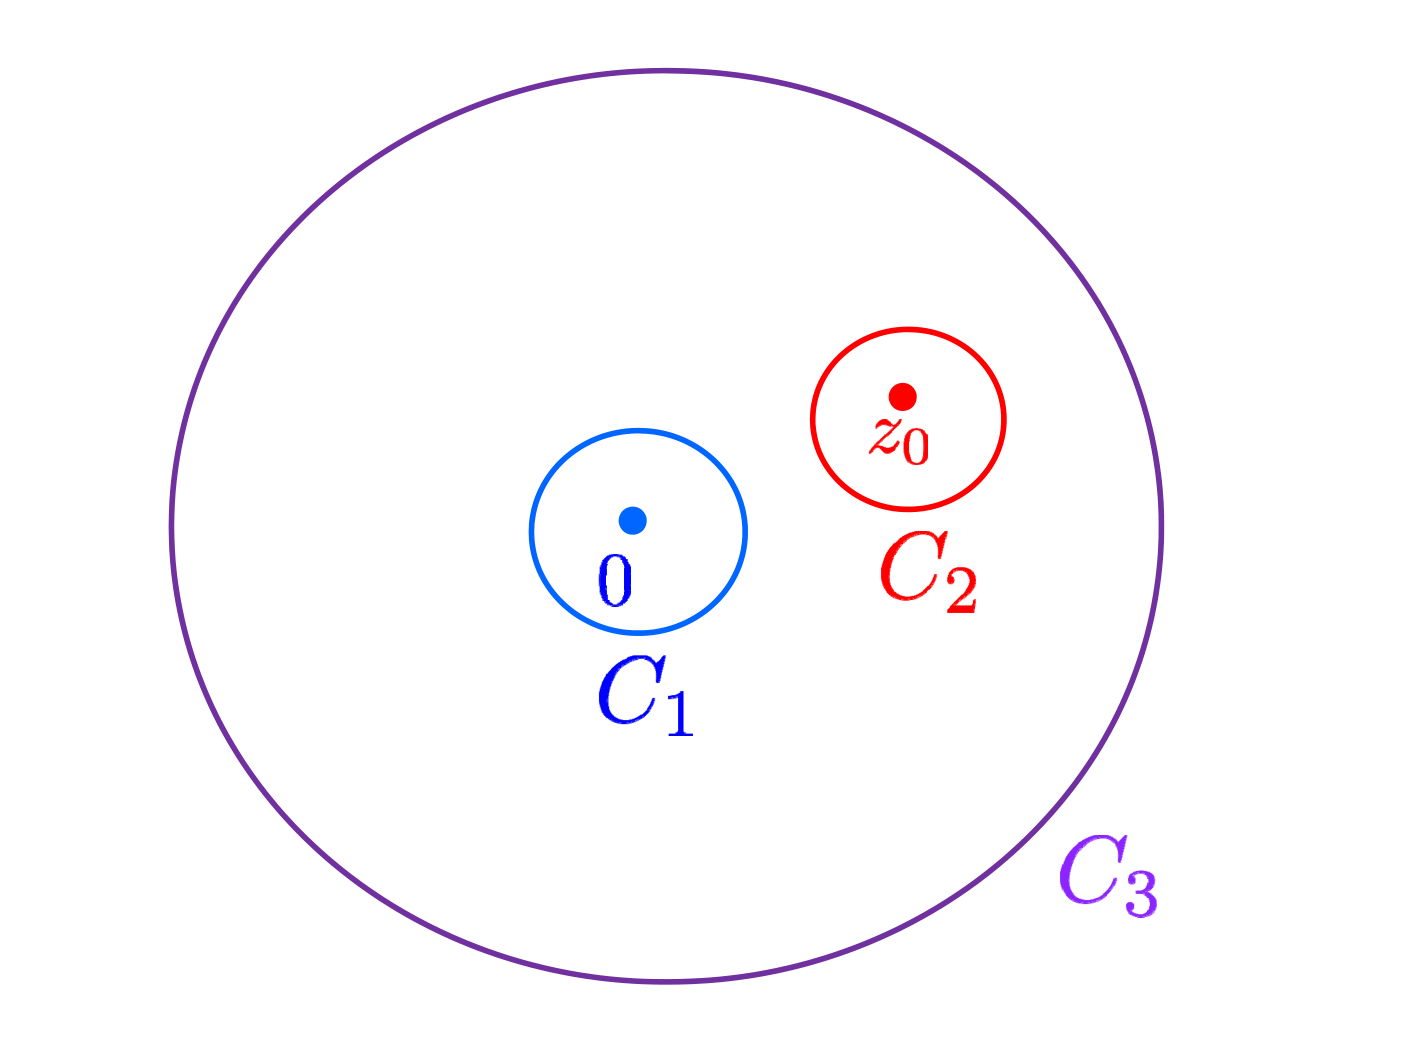
\includegraphics[width=0.55\textwidth]{figures/fig19.png}
  \caption{三个 CFT 状态空间分别与圆 $C_1$、$C_2$、$C_3$ 相关联，它们分别对应于围绕 $z=0$、$z_0$、$0$ 的径向量子化。（原文 Fig.~19，第 140 页）}
  \label{fig:19}
\end{figure}

\subsection{最高权表示的张量积} % 原文: 4.8 Tensor Product Of Highest Weight Representations

可积最高权表示 $L(\lambda)$ 原来是张量范畴（tensor category）中的对象。张量积并不是对称的。注意，要取两个表示 $L(\lambda)$ 与 $L(\lambda')$ 的张量积、以得到同一个 $k$ 值的 KM 代数的表示，这并非显然。\footnote{出于同样的理由，人们也不愿意把特征标相乘。} 做到这一点的办法是利用共形场论。

张量积可以这样理解。（我们沿用 [42] 式 (2.5) 的描述。利用顶点算符代数理论对张量积的严格描述见 [29, 30]。）

我们可以构造一个流：
\begin{equation}
  J^a(z)=\sum T_n^a z^{-n-1}dz
  \tag{4.217}
  \label{eq:4.217}
\end{equation}
其中我们现在把 $z$ 解析延拓到复平面——把它看作 WZW 模型的二维欧氏 QFT 的欧氏世界面。注意
\begin{equation}
  T_n^a=\oint z^nJ^a(z)
  \tag{4.218}
  \label{eq:4.218}
\end{equation}

存在态–算符对应：在平面上的点 $z$ 处插入一个局部算符 $\Phi(z)$，会在以该点为中心的径向量子化的 Hilbert 空间中产生一个态。

要给出张量积，我们需要一个余乘法（comultiplication）$\Delta:\mathcal{A}\to\mathcal{A}\otimes\mathcal{A}$，其中 $\mathcal{A}$ 是局部可观测量的代数。

设想：在以 $z=0$ 为中心的小圆 $C_1$ 上有第一个态的 Hilbert 空间，在以 $z=z_0$ 为中心的第二个圆 $C_2$ 上有第二个，而在以 $z=0$ 为中心、但环绕 $z_0$ 的第三个更大的圆 $C_3$ 上有第三个。见图~\ref{fig:19}。

若在 $z=0$ 与 $z=z_0$ 处插入在表示 $L_\lambda$ 与 $L_\mu$ 中产生态的局部算符，则圆 $C_3$ 上所得到的态将带有流的作用，其模为
\begin{equation}
  \begin{aligned}
    \Delta_{0,z_0}(T_n^a)&=\oint_{C_3}z^nJ^a(z)\\
    &=\left(\oint_{C_1}z^nJ^a(z)\right)\otimes 1+1\otimes\left(\oint_{C_2}z^nJ^a(z)\right)
  \end{aligned}
  \tag{4.219}
  \label{eq:4.219}
\end{equation}
第一行写的是作用在圆 $C_3$ 上态空间的一个算符。（可以把它想成一条裤子图（pair of pants）中的出射态空间。）下一行是一次围道形变（因为 $J^a(z)$ 是全纯流），以给出对圆 $C_1$ 与 $C_2$ 上态空间的作用。由于裤子图上有两个入射态，我们得到的是态空间的张量积。有趣的一项是 $\oint_{C_2}z^nJ^a(z)\,dz$。当作用在以 $z_0$ 为中心的径向量子化所得的 Hilbert 空间上时，我们应把流展开为
\begin{equation}
  J^a(z)=\sum_{m\in\mathbb{Z}}(z-z_0)^{-m-1}J_m^a(z_0)\,d(z-z_0)
  \tag{4.220}
  \label{eq:4.220}
\end{equation}
但
\begin{equation}
  \oint_{C_2}z^n(z-z_0)^{-m-1}dz=
  \begin{cases}
    0 & m\le-1\\
    \binom{n}{m}z_0^{n-m} & m\ge0
  \end{cases}
  \tag{4.221}
  \label{eq:4.221}
\end{equation}
从而
\begin{equation}
  \Delta_{0,z_0}(T_n^a)=T_n^a\otimes 1+1\otimes\left(\sum_{k=0}^{\infty}\binom{n}{k}z_0^{n-k}T_k^a(z_0)\right)
  \tag{4.222}
  \label{eq:4.222}
\end{equation}
% [Tutor Note: (4.221) 的二项式系数来自留数而非展开系数的直接读取：(4.220) 的展开点是 $z_0$，而围道积分号里带的是 $z^n=((z-z_0)+z_0)^n$，其 $z_0^{n-m}(z-z_0)^m$ 项与 $(z-z_0)^{-m-1}$ 相乘后给出 $(z-z_0)^{-1}$ 的留数，故系数为 $\binom{n}{m}z_0^{n-m}$；同时 (4.220) 的微分是 $d(z-z_0)$ 而文中被积式写的是 $dz$，两者相等，但若误把 (4.220) 的 $dz$ 漏掉就会丢掉 $(z-z_0)^{-m-1}$ 这一幂次的来源。此外 (4.222) 中的 $T_k^a(z_0)$ 带上了展开点 $z_0$，与 (4.217) 中无自变量的 $T_n^a$ 不是同一个记号，对照时勿混]

现在，简单对象（即 $G_k$ 的不可约表示）在这一张量积下的乘法融合规则，原来定义出一个半单 Frobenius 代数：\footnote{其概念上的理由是：可以把 WZW 模型的 $G$ 对称性规范化，从而得到 $G/G$ 模型。这是一个二维 TFT。}
\begin{equation}
  L(\mu)\otimes_{0,z_0}L(\nu)\cong\oplus_\lambda N_{\mu\nu}^{\ \ \lambda}L(\lambda).
  \tag{4.223}
  \label{eq:4.223}
\end{equation}

因此，存在一个矩阵 $S$ 对角化这些规则。
% [Tutor Note: 原文用 "turn out to define" 一笔带过 (4.223) 中「半单性 + Frobenius 结构」的验证，被省略的实质内容是：$G_k$（能级 $k$ 的仿射 KM 代数）的可积表示在共形场论给出的张量积下融合系数非负、结合（由共形块的结合律 / 五边形方程保证），且存在非退化不变配对使融合代数成为半单 Frobenius 代数——这正是 Verlinde 公式成立的前提。作者在脚注中提示的 $G/G$ 模型给出的是一条概念性论证思路；严格证明可查 [42] 所引的文献，以及本章前文关于 $S$ 矩阵与融合规则关系的讨论]

% =====================================================================
%  c17 —— 原文印刷页 142–148（PDF 第 143–149 页）
%  含：4.8.1 Fusion Rules For The WZW Model、4.9 Conformal Blocks And
%  Monodromy、4.10 Open String WZW Model、第 5 章开头（5. Topological Field
%  Theories And Categories）及 5.1 Basic Ideas；插图 Fig. 20–22。
%  编号公式 (4.224)–(4.236)、(5.1)–(5.5)。
% =====================================================================

\subsubsection{WZW 模型的融合规则} % 原文: 4.8.1 Fusion Rules For The WZW Model

一般而言，若用 $G$ 的表示在 $L_0$ 最低本征值处的支配权（dominant weight）来标记 $G_k$ 的各不可约最高权表示，则相应的本征值为
\begin{equation}
  \Lambda^{(\mu)}_\nu=\frac{S_\mu^{\ \nu}}{S_0^{\ \nu}}=\mathrm{ch}_\mu\left(2\pi\frac{\nu+\rho}{k+h}\right)
  \tag{4.224}
  \label{eq:4.224}
\end{equation}
其中 $\mu,\nu$ 是支配权，$\rho$ 是 Weyl 向量，\footnote{Weyl 向量是全部正根之和的一半，它也等于各基本权之和。} $h$ 是对偶 Coxeter 数；并且我们已经用按 $(\theta,\theta)=2$ 归一化的 Killing 型把 $\mathrm{t}^{\vee}$ 与 $\mathrm{t}$ 等同起来，从而把 $\nu+\rho$ 看成 $\mathrm{t}$ 中的一个元素。
% [Tutor Note: (4.224) 的 $S$ 矩阵把第二个指标排成了上标：$\frac{S_\mu^{\ \nu}}{S_0^{\ \nu}}$ 应读作 $S_{\mu\nu}/S_{0\nu}$（行指标 $\mu$、列指标 $\nu$，列指标在这里被 Killing 型「抬高」），并不是 $S^{\nu}_{\ \mu}$。这套「错位」排法与 (4.190)、(4.197) 中的 $S_\nu^{\ x}$、$S_0^{\ x}$ 是同一套约定：只有 \ 空位之后出现的那个指标，才与前面的指标配对。另需注意，分母 $S_0^{\ \nu}$ 与下文 (4.225)–(4.227) 用的是同一个矩阵，而按原文 p.136 的讨论，$S$ 的整体归一化在此之前并未被固定，因此若要把 (4.224) 与 (4.201) 的数值直接对照，须先统一归一化，否则会差一个与 $\nu$ 无关的因子。]
{\small\itshape ［原文标记：请给出本公式对 $SU(2)_k$ 的特殊化。］}
% [原文待办标记，原文 p.142；位于右侧页边，以 \ensuremath{\clubsuit} 号括起]

利用 \eqref{eq:4.224}，可以把 CFT 的融合规则 $N^{\lambda}_{\mu\nu}$ 用有限维群的 Littlewood–Richardson 系数 $\bar N^{\lambda}_{\mu\nu}$ 表示出来：
\begin{equation}
  \mathrm{ch}_\mu\mathrm{ch}_\nu=\sum_{\lambda\in\Lambda^{+}_{wt}}\bar N^{\lambda}_{\mu\nu}\mathrm{ch}_\lambda
  \tag{4.225}
  \label{eq:4.225}
\end{equation}

我们知道，对半单 Frobenius 代数一般有
\begin{equation}
  \Lambda^{(\mu)}_x\Lambda^{(\nu)}_x=\sum_\lambda N^{\lambda}_{\mu\nu}\Lambda^{(\lambda)}_x
  \tag{4.226}
  \label{eq:4.226}
\end{equation}

把 \eqref{eq:4.225} 在特殊的共轭类 $2\pi(\lambda+\rho)/(k+h)$ 上取值，并作一些简单的运算，\footnote{见 Di Francesco 等，第 16.2.1 节；或 Fuchs，第 5.5 节。}便得到
\begin{equation}
  N^{\lambda}_{\mu\nu}=\sum_{w\in\widehat{W}^{k},\;w\cdot\lambda\in\Lambda^{+}_{wt}}\operatorname{sign}(w)\,\bar N^{w\cdot\lambda}_{\mu\nu}
  \tag{4.227}
  \label{eq:4.227}
\end{equation}
（$w$ 的符号是有定义的，因为 $\widehat{W}^{k}$ 是 Coxeter 群：按该群元素是偶数个还是奇数个反射的乘积，它取 $\pm1$。）
% [Tutor Note: (4.227) 里的「$\cdot$」是仿射 Weyl 群的平移作用（dot action）$w\cdot\lambda=w(\lambda+\rho)-\rho$，作者没有写出定义，只说「simple manipulations」；不写出这一步就无法看出为何求和指标要限制在 $w\cdot\lambda\in\Lambda^{+}_{wt}$ 上，也无法看出该求和是有限项（$\widehat W^k$ 虽无限，但使 $w\cdot\lambda$ 落在支配 Weyl 腔内的元素只有有限多个，这正是 (4.229) 里 $k-j-j'$ 那条截断的来源）。此外 $\operatorname{sign}(w)=\det(w)$，因为 $\widehat W^k$ 是反射生成的 Coxeter 群，其符号同态有定义，$w\cdot\lambda$ 落在 Weyl 腔壁上时应按重数处理，不能简单逐项相加。]

例如，对 $SU(2)_k$，通常的 Clebsch–Gordon 规则 $\bar N^{j''}_{jj'}$ 给出
\begin{equation}
  [j]\otimes[j']=[|j-j'|]\oplus[|j-j'|+1]\oplus\cdots\oplus[j+j']
  \tag{4.228}
  \label{eq:4.228}
\end{equation}
然而，若 $j+j'>k/2$，则在 $j=k/2$ 附近会出现一个仿射 Weyl 反射。每个大于 $k-j-j'$ 的权都会有一个大于 $k/2$ 的反射像，而这些项将成对抵消。如此便得到
\begin{equation}
  N^{j''}_{jj'}=
  \begin{cases}
    1 & |j-j'|\le j''\le\min\{j+j',\,k-j-j'\}\;\&\;j+j'+j''\in\mathbb{Z}\\
    0 & \text{else}
  \end{cases}
  \tag{4.229}
  \label{eq:4.229}
\end{equation}
% [Tutor Note: (4.229) 第一行的条件之间，原文印的是逻辑与符号「&」而不是逗号或 "and"——这是作者把源码里的对齐符误排进了正文（同一符号在 (4.227) 的求和下标里也被用作分隔）。译文照原样保留 \&，读作「并且」。另需注意 $[j]$ 表示自旋 $j$ 的表示，方括号不是绝对值；条件 $j+j'+j''\in\mathbb{Z}$ 保证三个权之和为整数，即 $SU(2)$ 的「三角形」条件在仿射截断下仍成立。]
{\small\itshape ［原文标记：关于四面体（tetrahedra）说点什么。］}
% [原文待办标记，原文 p.142；位于 (4.229) 右侧页边，以 \ensuremath{\clubsuit} 号括起；指的应是 6j 符号/四面体网络与融合矩阵的关系]

\textbf{练习}
\begin{enumerate}[label=\alph*.)]
  \item 求出由 $N^{j''}_{jj'}$ 定义的 Frobenius 代数的诸不变量 $\theta_x$。
  \item 注意：由于 $N^{j''}_{jj'}$ 是整数，$Z(\Sigma_g)$ 也是整数——若把它看成 \eqref{eq:4.199}，这是一个令人惊讶的事实。它是著名的 Verlinde 公式的一个特例。
\end{enumerate}
% 备考（非批注，仅备核查）：练习 b.) 引用的 \eqref{eq:4.199} 即 $Z_g=\sum_x\theta_x^{1-g}$。
% 「整数性」要把 $\sum_x\theta_x^{1-g}$ 按 Verlinde 公式改写为对融合系数 $N$ 的多重求和，
% 于是 $Z(\Sigma_g)$ 变成若干整数（融合系数的乘积）之和——这才是 "surprising" 的确切含义。

% [原文标记：此处有两条细横线，为原稿的分段记号，原文 p.143]

\textbf{练习}
\begin{enumerate}[label=\alph*.)]
  \item 证明：能级 $k$ 与能级 $k'$ 的 theta 函数之积（作为 $z$ 的函数）可以按能级 $k+k'$ 的 theta 函数展开。于是，取能级 $k$ 的 theta 函数所张成空间的直和，便定义出一个分次环（graded ring）。
  \item 证明：特征标 $\chi^k_j(z,\tau)$ 可以按能级 $k$ 的 theta 函数展开。
\end{enumerate}

这是看待「$SU(2)_k$ 的表示在通常张量积下不会给出 $SU(2)_k$ 的表示」这一事实的另一条途径。

\subsection{共形块与单值性} % 原文: 4.9 Conformal Blocks And Monodromy

共形块的单值性（monodromy）：编织矩阵 $B$；自洽性：编织关系（braid relations）。

共形块空间的维数公式。

更高亏格上的共形块：Riemann 面模空间上的射影平坦联络。Sugawara 与平行移动。

\subsection{开弦 WZW 模型：保对称的边界条件} % 原文: 4.10 Open String WZW Model: Symmetry Preserving Boundary Conditions

开弦与膜（branes）：共轭类。保对称的 D-膜（即边界条件）。

当时空 $\mathcal{S}_{2n}$ 不是闭的、而是带边界的流形时，WZ 项的性质会变得微妙得多。我们将在下文对此作些评论。

不过，现在就可以讨论运动方程的解，而不必陷入构造作用量的那些微妙之处。让我们在二维情形中说明这一点：

我们的场定义为 $g(\sigma,t)$，其中 $\sigma\in[0,\pi]$。

我们取作用量为 $kS^{+}_{\mathrm{WZW}}$，于是守恒流为
\begin{equation}
  \begin{aligned}
    \partial_+J_R(x^-)=0 &\qquad J_R=g^{-1}\partial_-g\\
    \partial_-J_L(x^+)=0 &\qquad J_L=\partial_+gg^{-1}
  \end{aligned}
  \tag{4.230}
  \label{eq:4.230}
\end{equation}
其中 $x^{\pm}=t\pm\sigma$。
% [Tutor Note: (4.230) 两式的 $\partial_+$ 与 $\partial_-$ 极易写反：$J_R=g^{-1}\partial_-g$ 只依赖 $x^-$，故守恒律为 $\partial_+J_R=0$（右行扇区）；$J_L=\partial_+gg^{-1}$ 只依赖 $x^+$，故守恒律为 $\partial_-J_L=0$（左行扇区）——出现守恒律里的那个导数方向，总与流自身携带的那个 $\partial$ 相反。另注意 $R,L$ 指的是世界面 $(\sigma,t)$ 上的右行/左行方向，与群的左右作用无关；又因 $g$ 取值在非阿贝尔群中，$g^{-1}\partial_-g$ 与 $\partial_+gg^{-1}$ 的因子次序不可交换，逐式核对时须保持原序。]

我们已经看到，运动方程的通解为
\begin{equation}
  g(t,\sigma)=g_L(x^+)g_R(x^-)
  \tag{4.231}
  \label{eq:4.231}
\end{equation}

但现在我们应当选取边界条件。一类自然的边界条件是在 $\sigma=0$ 处的「保对称」边界条件，它说的是总的 $J_\sigma$ 流不应从侧面漏出：
\begin{equation}
  (J^{(L)}+J^{(R)})_\sigma=0\;\Rightarrow\;g'_L(t)g_L^{-1}(t)=-g_R^{-1}(t)g'_R(t)
  \tag{4.232}
  \label{eq:4.232}
\end{equation}

因此，存在某个取值为 $\mathbf{g}$ 的时间函数 $A(t)$，使得
\begin{equation}
  \begin{aligned}
    g'_L(t)&=A(t)g_L(t)\\
    g'_R(t)&=-g_R(t)A(t)
  \end{aligned}
  \tag{4.233}
  \label{eq:4.233}
\end{equation}
用路径排序指数（path-ordered exponential）积分，我们得到
\begin{equation}
  A(t)=\partial_tUU^{-1}=-U\partial_t(U^{-1})
  \tag{4.234}
  \label{eq:4.234}
\end{equation}
于是通解为
\begin{equation}
  \begin{aligned}
    g_L(t)&=U(t)g_L(0)\\
    g_R(t)&=g_R(0)U^{-1}(t)
  \end{aligned}
  \tag{4.235}
  \label{eq:4.235}
\end{equation}
从而
\begin{equation}
  g(t)=g_L(t)g_R(t)=U(t)g_L(0)g_R(0)U^{-1}(t)=U(t)g(0)U^{-1}(t)
  \tag{4.236}
  \label{eq:4.236}
\end{equation}
% [Tutor Note: 从 (4.232) 到 (4.233) 的一步被作者用 "there is some ... function" 一句带过：由 (4.232) 两端相等，可令 $A(t):=g'_L(t)g_L^{-1}(t)=-g_R^{-1}(t)g'_R(t)$ 为同一个 $\mathbf{g}$-值时间函数，(4.233) 的两式就是它的改写；$A$ 只依赖 $t$、与 $\sigma$ 无关，这一点用的是 (4.231) 的乘积形式加边界条件。(4.234) 等价于 $\partial_tU=A(t)U$ 的解 $U(t)=P\exp\int_0^tA$（$P$ 为路径排序），而 $A=\partial_tUU^{-1}=-U\partial_t(U^{-1})$ 的后一等式由 $0=\partial_t(UU^{-1})$ 推出。(4.235) 的第二式中 $g_R$ 带的是 $U^{-1}$：代入 $g'_R=-g_RA$ 恰好成立，若写成 $U$，符号与次序都会出错——这是全推导中最容易抄错的一步。]
% [Tutor Note: (4.236) 只用到了 $\sigma=0$ 端的边界条件，$\sigma=\pi$ 端的条件原文尚未讨论；因此这里的结论是「开弦一端沿共轭类运动」，要谈两端都落在（可能不同的）共轭类上，还需要在 $\sigma=\pi$ 处再取一个保对称边界条件。]

因此，\emph{开弦的两端沿群中的一条共轭类运动}。
% [原文原文为 "the ends of the the open string"，"the" 重复，系原稿笔误，译文只保留一个]

{\small\itshape ［原文标记：此处应为 $SU(2)$ 的插图（原 PDF 中只有一行占位文字，未插入图形）。］}
% [原文待办标记，原文 p.144；原文此行仅为 "FIGURE FOR SU2" 占位]

在量子理论中（对紧致群而言），结果发现允许的共轭类本身也被量子化了。关于开弦 WZW 模型的一些参考文献见：

\begin{enumerate}
  \item Volker Schomerus, “Lectures on branes in curved backgrounds,” Class.Quant.Grav.19:5781-5847,2002. e-Print: hep-th/0209241
  \item G. Moore, “K theory from a physical perspective,” e-Print: hep-th/0304018
\end{enumerate}

{\small\itshape ［原文标记：关于 Freed–Hopkins–Teleman 定理的评论（待写）。］}
% [原文待办标记，原文 p.144；原文以整行星号将该行上下框住]

\section{拓扑场论与范畴} % 原文: 5. Topological Field Theories And Categories

\begin{keytakeaways}
  \item 关联（association）：TFT 的基本数据是把 $(d-1)$ 维空间 $Y$ 指派为态空间 $\mathcal{H}(Y)$，把 $d$ 维配边 $X:Y\to Y'$ 指派为线性映射 $F(X):\mathcal{H}(Y)\to\mathcal{H}(Y')$；相对边界同胚的配边给出同一个映射，故这些数据只依赖拓扑。
  \item 乘性公理：\eqref{eq:5.3} 把无交并变成张量积，$\mathcal{H}(\varnothing)=\mathbb{C}$ 是单位；这与代数拓扑中上同调对无交并取直和的做法正相反，作者正是以此解释「量子不变量」这一称呼的由来。
  \item 对称结构：\eqref{eq:5.4} 的交换同胚给出 \eqref{eq:5.5} 的换位同构 $\Omega$；$Y$ 的自同胚则给出 $\mathcal{H}(Y)$ 上微分同胚群的一个（可能平凡的）表示——这是 TFT 中「时空对称性」的全部残留。
  \item 定域性只有一条：路径积分「对完备中间态求和」被形式化为配边的粘接性质，作者强调它在泛函积分表述中尤为显然；这是 Atiyah 公理中唯一真正用到「量子」的地方。
  \item 被刻意丢掉的结构：不要求 $\mathcal{H}(Y)$ 带内积（带内积的是幺正 TFT）、不要求度规与 Hamiltonian，因此 \eqref{eq:5.1}–\eqref{eq:5.5} 只是「物理理论」的最粗骨架，换个几何范畴即可套到任意场论上。
\end{keytakeaways}

{\small\itshape ［原文标记：只做到刚好能回到 CS 理论、走一遍手术（surgery）论证与 Verlinde 公式的「奥林匹克式证明」的程度即可。］}
% [原文待办标记，原文 p.144；原文为整段全大写指示，上下各有一行星号]

\subsection{基本想法} % 原文: 5.1 Basic Ideas

拓扑场论是引入物理学的某些基本思想、以及某些优美数学思想的极好的教学工具。

TFT 的想法源于两方面的研究：二维共形场论的研究，以及 Witten 关于 Donaldson 理论与 $N=2$ 超对称场论之关系的工作，和 Witten 关于 Jones 多项式与三维量子场论的工作。

\begin{figure}[htbp]
  \centering
  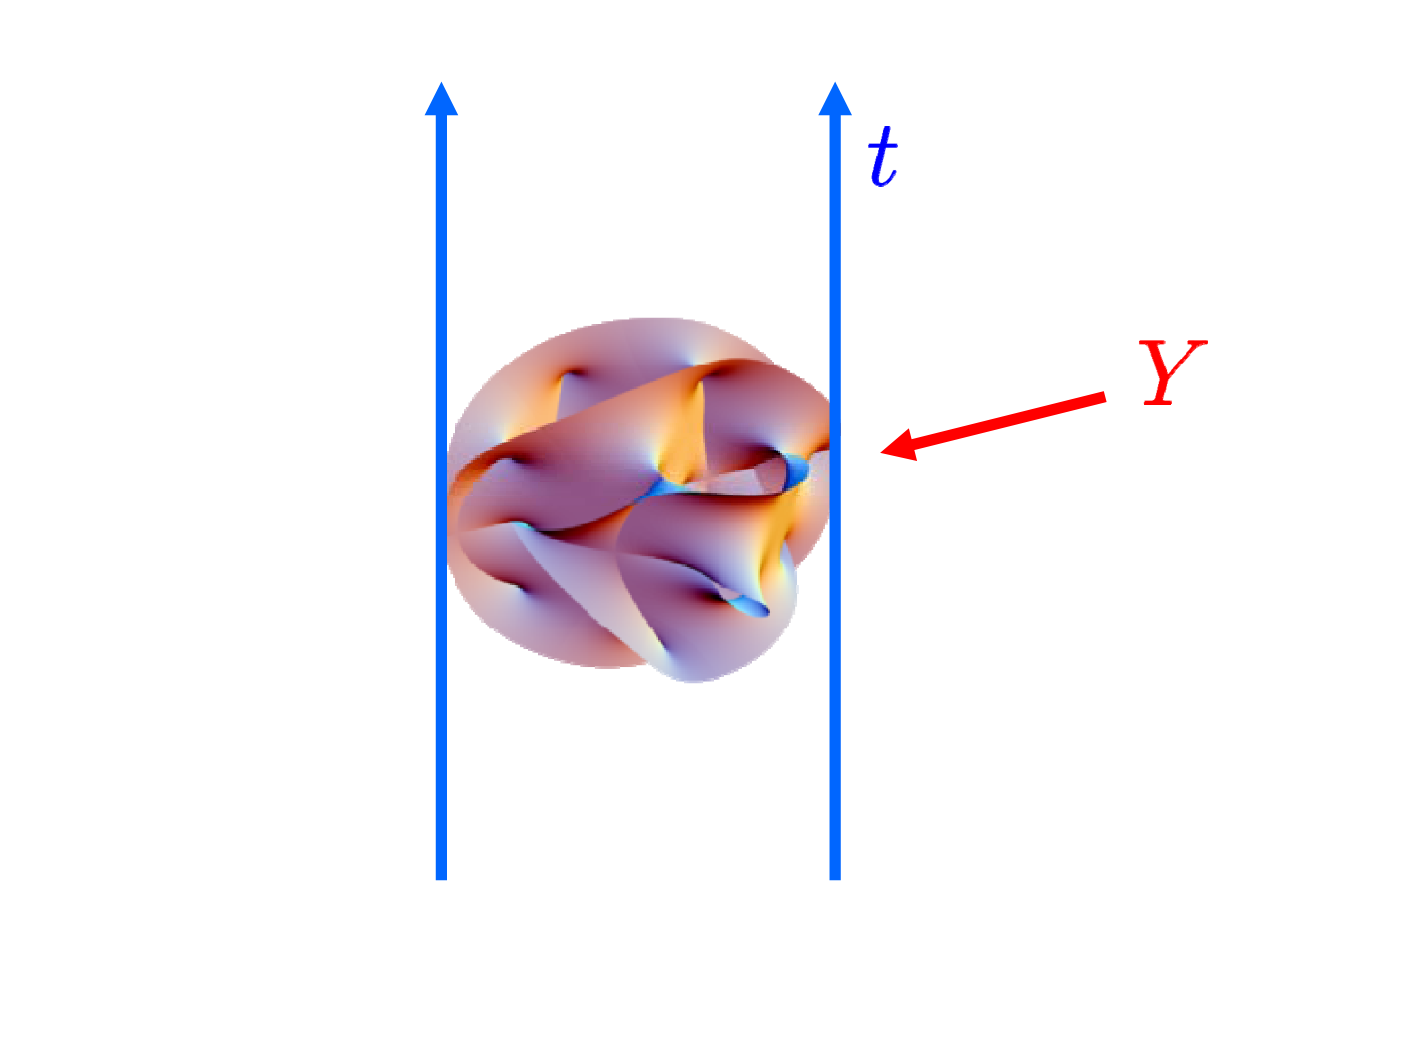
\includegraphics[width=0.62\textwidth]{figures/fig20.png}
  \caption{一个时空 $X_d=Y\times\mathbb{R}$。$Y$ 是 $(d-1)$ 维空间，可以具有非平凡的拓扑。（原文 Fig.~20，第 145 页）}
  \label{fig:20}
\end{figure}

在共形场论中，Graeme Segal 陈述了一组用以定义 CFT 的公理。Atiyah 把它们改造成 TFT 的定义。

TFT 可以看作物理学的一个基本框架。它把 Hilbert 空间、态与跃迁振幅指派给拓扑空间，其方式抓住了「定域性」最原始的那些含义。把「真实物理」的诸多复杂性剥离之后，剩下的结构非常简单。然而，所得的结构是优雅的：它与优美的代数结构相联系，而这些结构（至少在二维）有着出人意料地有用的推论。这是少数几个可以真正「解出理论」的场合之一。

当然，我们关心的是更复杂的理论。但这里的这个基本框架可以套用到任何场论上：变化的是所考虑的几何范畴。于是，它为「什么是量子场论？」这个一般性问题提供了一条进路。

谈论 0 维时空中的物理是可能的。从泛函积分的观点看，这非常自然：路径积分变成了通常的积分。考虑以 0 维时空为目标空间的弦论也很有收获。然而，在绝大多数物理问题中，我们处理的是 $d$ 维时空中的系统，$d>0$。以下我们假定 $d>0$。

在 $d$ 维时空中，我们想从一个物理理论得到的最原始的东西是什么？在一个物理理论中，人们常把时空分解为空间与时间，如图~\ref{fig:20} 所示。若空间是 $(d-1)$ 维流形 $Y$，那么在量子力学中，我们给它指派一个态空间，即向量空间 $\mathcal{H}(Y_{d-1})$。
% 原文此处把图的编号写作 "(20)"（即 Fig. 20），译文按图号引用

当然，在量子力学中 $\mathcal{H}(Y_{d-1})$ 通常带有更多结构——它是一个 Hilbert 空间。但本着「只发展最原始的部分」的精神，我们暂时不把这些结构纳入。（幺正 TFT 的概念才把 Hilbert 空间包含进来，见下文。）此外，在一个一般的物理理论中，还有作用在这个 Hilbert 空间上的自然算符，例如 Hamiltonian。Hamiltonian 的谱以及其他物理可观测量的谱依赖于大量数据。它们当然依赖于时空的度规，因为非零的能量定义了一个长度标度
\begin{equation*}
  L=\frac{\hbar c}{E}.
\end{equation*}
在拓扑场论中，人们忽略这一结构的大部分，而专注于 $\mathcal{H}(Y)$ 对 $Y$ 的拓扑的依赖。为简单起见，我们起初假定 $Y$ 是紧致无边流形。

于是：在拓扑场论中，我们希望有一个关联：$(d-1)$ 维流形 $Y$ 对应到向量空间，即 $Y\to\mathcal{H}(Y)$，使得「同胚的流形给出相同的 $\mathcal{H}(Y)$」。
% 原文作 "H(Y) is the same for homeomorphic vector spaces"，其中 "vector spaces" 显然应为 "manifolds"（同胚是流形之间的），系原稿笔误
这句话的意思是：若存在同胚
\begin{equation}
  \varphi:Y\to Y'
  \tag{5.1}
  \label{eq:5.1}
\end{equation}
则存在相应的向量空间同构
\begin{equation}
  \varphi_*:\mathcal{H}(Y)\to\mathcal{H}(Y')
  \tag{5.2}
  \label{eq:5.2}
\end{equation}
使得同胚的复合对应向量空间同构的复合。特别地，$Y$ 的自同胚作为 $\mathcal{H}(Y)$ 的自同构作用：于是它给出了微分同胚群的一个（可能平凡的）表示。

现在，我们还希望在最原始的水平上纳入某种形式的定域性。于是，若取无交并，则
\begin{equation}
  \mathcal{H}(Y_1\coprod Y_2)=\mathcal{H}(Y_1)\otimes\mathcal{H}(Y_2)
  \tag{5.3}
  \label{eq:5.3}
\end{equation}
注意 \eqref{eq:5.3} 意味着：应当把 $\mathcal{H}(\varnothing)$ 取作向量空间所在的基域（field of definition）。为简单起见，我们取 $\mathcal{H}(\varnothing)=\mathbb{C}$，尽管也可以使用其他基域。
% [Tutor Note: (5.3) 是整套公理中唯一的乘性公理，也是「拓扑不变量」与「量子不变量」之分水岭：它把集合层面的无交并（$\coprod$）变成线性代数层面的张量积（$\otimes$），并要求「空集给出单位对象 $\mathbb{C}$」，否则 (5.3) 在 $Y_2=\varnothing$ 时不成立。由此可推：若 $Y=Y_1\coprod Y_2$ 而 $\mathcal{H}(Y_i)$ 的维数分别为 $m_i$，则 $\dim\mathcal{H}(Y)=m_1m_2$ 而非 $m_1+m_2$——检验任何具体 TFT 的候选赋值时，先查这一条最快能筛掉错误答案。]

\textbf{注记}：在代数拓扑中，把 Abel 群或向量空间指派给一个拓扑空间是相当常见的做法。例如，上同调群就是这样做的。但在这里我们看到与标准代数拓扑例子的一大差别。在那些例子里，空间在无交并之下是\emph{相加}的。而在量子力学中，空间是\emph{相乘}的。这正是许多拓扑学家把由拓扑场论得到的拓扑不变量称为「量子不变量」的根本原因。
% 原文为无编号的 run-in "Remark:"，故此处不用 remark 环境（环境会自动编号），保留为加粗提示语

最后，存在一个显然的同胚
\begin{equation}
  Y\coprod Y'\cong Y'\coprod Y
  \tag{5.4}
  \label{eq:5.4}
\end{equation}
因此必须存在一个同构
\begin{equation}
  \Omega:\mathcal{H}(Y)\otimes\mathcal{H}(Y')\to\mathcal{H}(Y')\otimes\mathcal{H}(Y)
  \tag{5.5}
  \label{eq:5.5}
\end{equation}
% [Tutor Note: 从 \eqref{eq:5.4} 到 \eqref{eq:5.5} 作者写 "there must be"，中间用到的是 \eqref{eq:5.1}–\eqref{eq:5.2} 的函子性再加上 \eqref{eq:5.3}：由 \eqref{eq:5.4} 得 $\mathcal{H}(Y\coprod Y')\cong\mathcal{H}(Y'\coprod Y)$，两端各用一次 \eqref{eq:5.3} 即得 \eqref{eq:5.5}。注意 $\Omega$ 不是任意的：它与 \eqref{eq:5.2} 中 $\varphi_*$ 的复合必须与同胚的复合相容（函子性），并与结合约束满足五边形/六边形相干条件——这正是「对称张量范畴」中对称性的公理。作者只说「必须存在」，这些相干性条件要等到后文把 TFT 与张量范畴（乃至高阶范畴）对应起来时才补上。]

\begin{figure}[htbp]
  \centering
  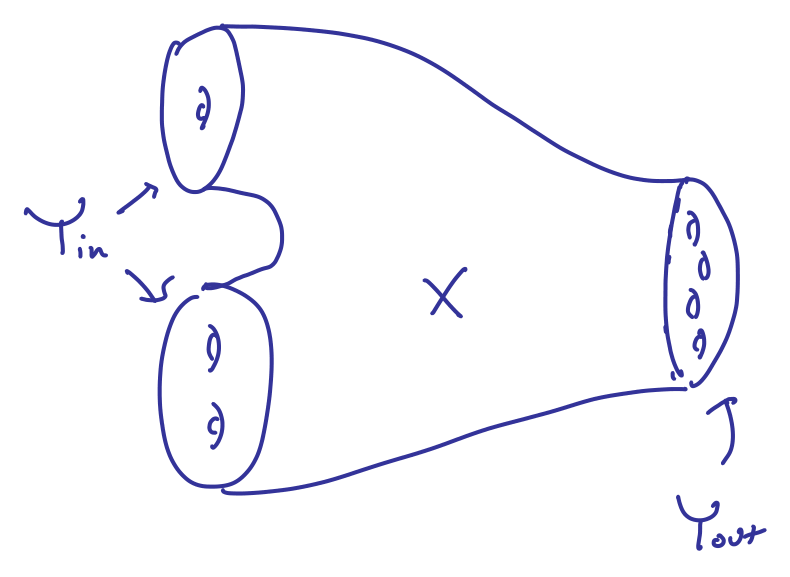
\includegraphics[width=0.68\textwidth]{figures/fig21.png}
  \caption{把乘积结构加以推广：一个 $d$ 维配边 $X$ 可以在初始的 $(d-1)$ 维空间切片 $Y_{\mathrm{in}}$ 与最终的空间切片 $Y_{\mathrm{out}}$ 之间包含拓扑的改变。由该配边上的路径积分所确定的振幅 $F(X)$ 是一个线性映射 $\mathcal{H}(Y_{\mathrm{in}})\to\mathcal{H}(Y_{\mathrm{out}})$。（原文 Fig.~21，第 147 页）}
  \label{fig:21}
\end{figure}

此外，在物理中我们还想谈论跃迁振幅。若有一个时空 $X_d$ 在两个时间切片之间插值，那么在数学上我们说 $Y$ 与 $Y'$ 之间存在一个配边（bordism）。也就是说，\emph{从 $Y$ 到 $Y'$ 的一个配边}是一个带边界的 $d$ 维流形，并且其边界被不交地分成两个集合，即「入边界」与「出边界」，
\begin{equation*}
  \partial X_d=(\partial X_d)_{\mathrm{in}}\cup(\partial X_d)_{\mathrm{out}}
\end{equation*}
使得有同胚 $(\partial X_d)_{\mathrm{in}}\cong Y$ 与 $(\partial X_d)_{\mathrm{out}}\cong Y'$。我们将在下文 {\small\itshape ［原文标记：Section ****，节号待补］} 中更精确地说明这一点，并讨论若干变体。
% [原文待办标记，原文 p.147；原文此处直接印出 "Section ****"，节号尚未填]

若 $X_d$ 是从 $Y$ 到 $Y'$ 的配边，则 Feynman 路径积分给出一个线性变换
\begin{equation*}
  F(X_d):\mathcal{H}(Y)\to\mathcal{H}(Y').
\end{equation*}
同样地，在一般情形下振幅依赖于 $X_d$ 的拓扑之外的大量数据；但在拓扑场论中，它们被认为只依赖于拓扑。

更精确地说，若 $X_d\cong X'_d$，且该同胚在配边的边界上等于恒等映射 $1$，则
\begin{equation*}
  F(X_d)=F(X'_d)
\end{equation*}

路径积分的一个关键方面——在量子力学中，或在量子场论中的泛函积分中，我们想要把握的（同样是定域性的一个推论）——是对完备中间态集合求和的想法。在路径积分表述中，我们可以这样来表述「从 $t_0$ 到 $t_2$ 对场构型的一切路径求和」：先把「从 $t_0$ 到 $t_1$ 的一切路径」与「从 $t_1$ 到 $t_2$ 的一切路径」的振幅复合起来（$t_0<t_1<t_2$），再对 $t_1$ 处的一切中间场构型求和。我们把这一性质称为「粘接性质」（gluing property）。粘接性质在场论的泛函积分表述中尤其显然。

\begin{figure}[htbp]
  \centering
  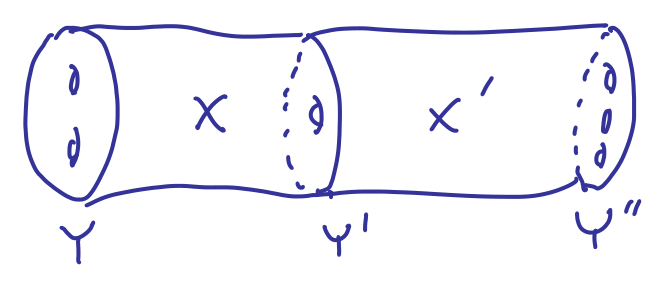
\includegraphics[width=0.55\textwidth]{figures/fig22.png}
  \caption{把两个配边粘接起来，得到第三个配边。（原文 Fig.~22，第 148 页）}
  \label{fig:22}
\end{figure}

在拓扑场论中，这被形式化为：

若 $X$ 是从 $Y$ 到 $Y'$ 的配边，且
\begin{equation*}
  (\partial X)_{\mathrm{in}}=Y\qquad(\partial X)_{\mathrm{out}}=Y'
\end{equation*}

% 本片段（印刷页 142–148）至此结束：原文在 p.148 页末中断于上述条件句，
% 其后的粘接公式与 5.1 节的剩余篇幅属于下一片段 c18。

% =====================================================================
%  c18 —— 原文印刷页 149–155（PDF 第 150–156 页）
%  含：5.1.1（三级标题）、5.2（二级标题）、5.2.1（三级标题）；
%  插图 Fig. 23–27；编号公式 (5.6)–(5.23)。
%  说明：本片段不含 \section 级标题（原文「5.2」为二级标题，按编号点数
%  对应 \subsection），故按规范不插入 keytakeaways。
% =====================================================================

而 $X'$ 是另一条从 $Y'$ 到 $Y''$ 的有向配边（bordism）
\begin{equation*}
  (\partial X')_{\mathrm{in}}=Y' \qquad (\partial X)_{\mathrm{out}}=Y''
\end{equation*}
那么我们便可如 {\small\itshape ［原文标记：(??)］} 那样作复合 $X'\circ X$，得到从 $Y$ 到 $Y''$ 的配边。
% [原文待办标记，原文 p.149：交叉引用未解析，页面显示为 (??)，所指应为附录 L 或正文前文中配边复合的定义式]
% [Tutor Note: 原文此处的两个边界条件写成 $(\partial X')_{\mathrm{in}}=Y'$ 与 $(\partial X)_{\mathrm{out}}=Y''$，第二式漏了撇号；按文意（$X'$ 是从 $Y'$ 到 $Y''$ 的配边）它应是 $(\partial X')_{\mathrm{out}}=Y''$。译文照原文转写、未擅自订正；对照第 148 页关于 $X:Y\to Y'$ 的边界约定即可确认这是笔误]

再自然不过的是，我们希望相应的线性映射也复合起来：
\begin{equation*}
  F(X'\circ X)=F(X')\circ F(X):\mathcal{H}(Y)\to\mathcal{H}(Y'')
\end{equation*}

我们所描述的，用数学术语说，就是范畴之间的一个函子（functor）。关于范畴的背景材料见附录 K。在描述了上述框架的若干变体之后，我们将更详细地解释这幅范畴论的图景。

\subsubsection{更多的结构} % 原文: 5.1.1 More Structure

我们可以把上述图景看作一个基本框架：通过充实与空间 $X$、$Y$ 相伴的拓扑数据与几何数据，就能在这个框架上造出更有趣的理论。

例如，我们或许能够给 $X$ 与 $Y$ 赋予

\begin{enumerate}
  \item 定向、spin、spin$^c$、pin 结构等（对某些 $X$ 与 $Y$）；
  \item 复结构、共形结构、因果结构、Riemann 结构；
  \item 其他的场——带联络的主 $G$-丛、相伴丛的截面等。
\end{enumerate}

动机性的例子之一是二维共形场论。在那一情形，Segal 的公理建立在赋有共形结构的二维配边之上。

在考虑非拓扑理论时，会出现两个重要的复杂之处：

\begin{enumerate}
  \item 标度（scale）与重整化的概念变得重要。
  \item Hilbert 空间其实并不是对某个 $(d-1)$ 维流形定义的，而是对 $(d-1)$ 维流形周围 $d$-流形的一个芽（germ）定义的；于是算符代数还可以依赖于额外的结构，例如第二基本形式。{\small\itshape ［原文标记：此处应引 Segal 以为例］}
% [原文待办标记，原文 p.149：原文作 [CITE SEGAL for example]，作者留待补引 Segal 关于共形场论公理化的文献]
\end{enumerate}

\subsection{拓扑场论的定义} % 原文: 5.2 The Definition Of Topological Field Theory

关于配边理论的基本数学背景，见 {\small\itshape ［原文标记：附录 ??］}。下文将假定读者对此已知晓。
% [原文待办标记，原文 p.149：原文作 See Appendix ??，交叉引用未解析（所指应为附录 L「Bordism」），且 backgound 一词在原文中拼写有误]

设 $S$ 是切丛上的一个结构，$C$ 是任一对称幺半范畴（symmetric monoidal category）。于是

\textbf{定义}：$S$-流形的 $d$ 维拓扑场论，是指从张量范畴 $\mathrm{Bord}^S_{\langle d-1,d\rangle}$ 到某个对称张量范畴 $C$ 的一个对称张量函子（symmetric tensor functor）。

我们一开始举的例子，就是 $S$ 为空、目标范畴为某个域 $\kappa$ 上的 $\mathrm{VECT}_\kappa$ 的情形；此时拓扑场论就是从 $\mathrm{Bord}_{\langle d-1,d\rangle}$ 到 $\mathrm{VECT}_\kappa$ 的张量函子。

关于这个更一般概念的若干例子：

\begin{enumerate}
  \item 用恒等函子！这就给出 Michael Freedman 所称的「懒汉式 TFT（lazy TFT）」，它导致流形的一种配对，具有非常有趣的正定性。见 {\small\itshape ［原文标记：[?]］}。
% [原文待办标记，原文 p.150：此处文献引用留空，原文作 See [?]]
  \item 我们可以如下推广。设 $K$ 是 $k$ 维闭流形，则与 $K$ 取笛卡儿积定义一个对称张量函子 $t_K$
\begin{equation}
  t_K:\mathrm{Bord}_{\langle d-1,d\rangle}\to\mathrm{Bord}_{\langle d+k-1,d+k\rangle}
  \tag{5.6}
  \label{eq:5.6}
\end{equation}
其中 $t_K(Y)=Y\times K$，如此等等。若 $F$ 是一个 $(d+k)$ 维 TFT，则可以复合 $F\circ t_K$，得到 $d$ 维 TFT，记作 $F^{KK}$。这是「Kaluza-Klein 紧致化」在拓扑场论中的类比。例如，$(d-1)$-流形上的态空间是
\begin{equation}
  F^{KK}(Y):=F(Y\times K)
  \tag{5.7}
  \label{eq:5.7}
\end{equation}
% 转写说明：上标 $KK$ 是「Kaluza-Klein」的缩写而非指标；$\mathrm{Bord}_{\langle d-1,d\rangle}$ 的下标是一整块的 $\langle d-1,d\rangle$，表示「对象为 $(d-1)$ 维、态射为 $d$ 维」的那一档配边，与 \eqref{eq:5.6} 右边的 $\langle d+k-1,d+k\rangle$ 逐项相差 $k$，不要写成普通圆括号。
  \item 如果存在足够自然的、依赖于某个几何范畴的量子场论构造，那么就可以定义一个 TFT，其取值是那个量子场论的真空模空间。在目标范畴取为全纯辛簇（holomorphic symplectic variety）的情形，这件事已在 {\small\itshape ［原文标记：[?]］} 中做到。
% [原文待办标记，原文 p.150：此处文献引用留空，原文作 in [?]]
\end{enumerate}

\subsubsection{一些一般性质} % 原文: 5.2.1 Some General Properties

让我们从上述简单评注推出一些简单的一般事实。

眼下先把目标范畴取为 $\mathrm{SVECT}_\kappa$，即域 $\kappa$ 上的超向量空间范畴。（若愿意，尽可忽略那些符号，直接用向量空间范畴来做。）

首先注意，若 $X$ 是闭的，则它可以看作从 $\emptyset$ 到 $\emptyset$ 的配边。因此 $F(X)$ 必须是从 $\kappa$ 到 $\kappa$ 的线性映射。但任何线性映射 $T\in\operatorname{Hom}(\kappa,\kappa)$ 都必呈如下形式
\begin{equation}
  T(z)=tz
  \tag{5.8}
  \label{eq:5.8}
\end{equation}
其中 $t\in\kappa$ 是某个标量。也就是说，任何线性映射 $\kappa\to\kappa$ 都典范地联系于基域中的一个元素。对 $F(X):\kappa\to\kappa$ 这种情形，我们把这个数称为 $X$ 的\emph{配分函数}（partition function），记作 $Z(X)$。

有一条配边是特殊的，即 $[0,1]\times Y$。它对应一个线性映射 $P:\mathcal{H}(Y)\to\mathcal{H}(Y)$。在欧氏场论中，人们会联系到柱状时空 $[0,1]\times Y$ 的振幅就是
\begin{equation*}
  \exp[-TH]
\end{equation*}
其中 $H$ 是 Hamilton 量，$T$ 是欧氏时间间隔。注意这需要一个度规。改变柱的长度会导致 $T$ 的改变。

显然，由拓扑场论的公理，$P^2=P$，因此我们可以分解
\begin{equation}
  \mathcal{H}(Y)=P\mathcal{H}(Y)\oplus(1-P)\mathcal{H}(Y)
  \tag{5.9}
  \label{eq:5.9}
\end{equation}
在第二个直和项上，所有跃迁都为零，因为从拓扑上看，我们总可以把这样一个柱插进去。由此可知，自然地应当假设
\begin{equation}
  F(Y\times[0,1])=Id_{\mathcal{H}(Y)}
  \tag{5.10}
  \label{eq:5.10}
\end{equation}
人们可以把它看作「Hamilton 量为零」这一陈述。注意这使得振幅与柱的长度无关。
% [Tutor Note: 从 $P^2=P$ 到 \eqref{eq:5.10} 之间，作者只用 "natural to assume" 一句带过了一步：公理只保证 $P$ 是一个投影（两条柱粘起来与一条柱同胚），而「所有跃迁在第二个直和项上为零」说的是 $P$ 在物理态上不起作用，于是可以重新归一化态空间（只保留 $P\mathcal{H}(Y)$）并令 $P=Id$。另需注意：原文用花体 $\mathcal{H}(Y)$ 记态空间，而 $H$ 同时用作 Hamilton 量（见 \eqref{eq:5.19} 的 $e^{-\beta H}$），两者字形与含义都不同，转写时不可混用]

\begin{figure}[htbp]
  \centering
  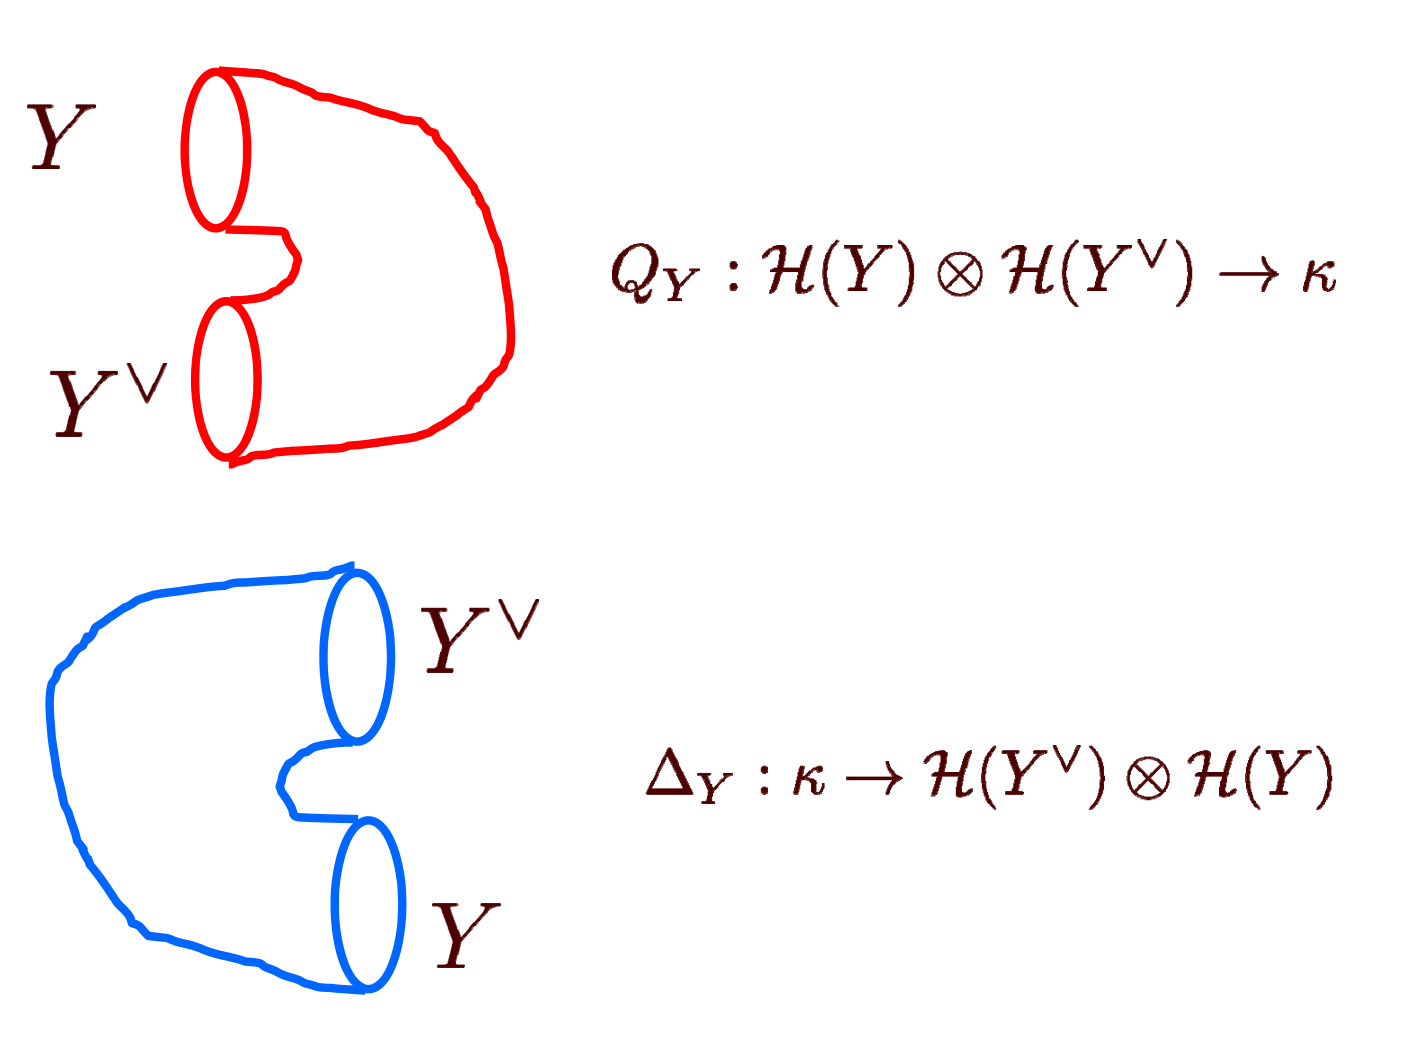
\includegraphics[width=0.50\textwidth]{figures/fig23.png}
  \caption{把柱弯折过来，以定义 $\Delta_Y$ 与 $Q_Y$。（原文 Fig.~23，第 151 页）}
  \label{fig:23}
\end{figure}

现在，让我们考虑有向配边范畴，于是 $Y$ 是有向的。以 $Y^\vee$ 记 $Y$ 取相反定向。配边 \eqref{eq:5.10} 与配边 $\emptyset\to Y^\vee\amalg Y$ 密切相关，后者定义一个映射
\begin{equation}
  \Delta_Y:\kappa\to\mathcal{H}(Y^\vee)\otimes\mathcal{H}(Y)
  \tag{5.11}
  \label{eq:5.11}
\end{equation}
它也与配边 $Y\amalg Y^\vee\to\emptyset$ 密切相关，后者定义一个二次型：
\begin{equation}
  Q_Y:\mathcal{H}(Y)\otimes\mathcal{H}(Y^\vee)\to\kappa
  \tag{5.12}
  \label{eq:5.12}
\end{equation}
现在把这些配边复合起来，我们就得到恒等映射，如图~\ref{fig:24} 所示。
% [原文此处作 "as in 24"（漏写了 Figure 一词），译文补出「图」字以便阅读]
于是由一些线性代数可知，$Q$ 是一个\emph{非退化}配对，从而我们有一个到线性对偶空间的同构：
\begin{equation*}
  \mathcal{H}(Y^\vee)\cong\mathcal{H}(Y)^\vee,
\end{equation*}

\begin{figure}[htbp]
  \centering
  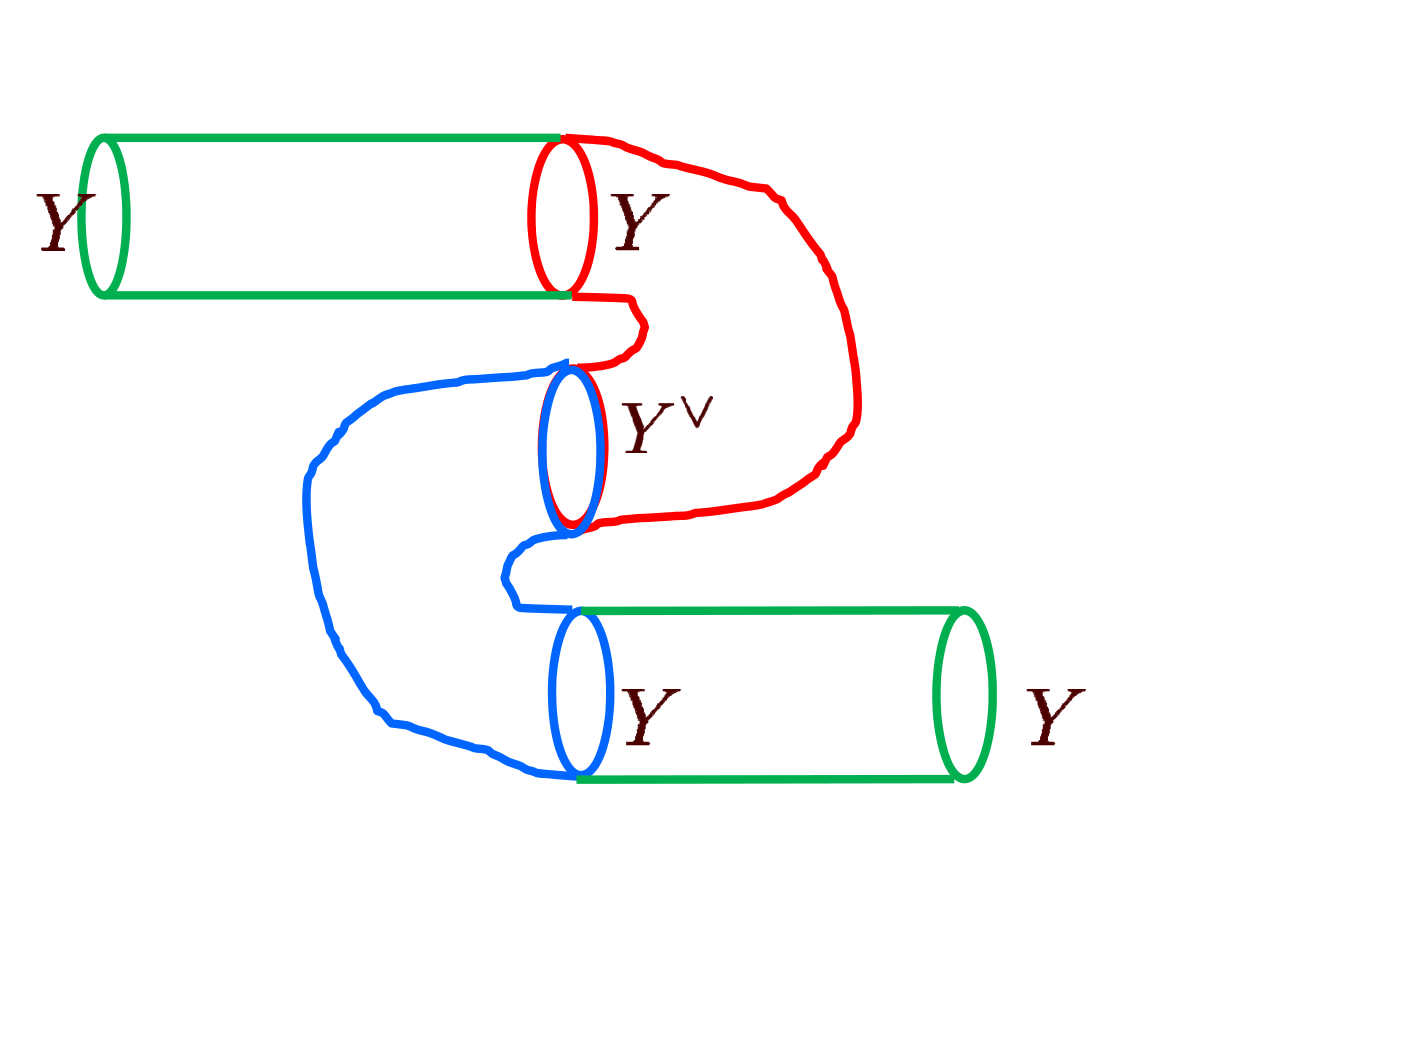
\includegraphics[width=0.50\textwidth]{figures/fig24.png}
  \caption{以某种方式复合 $\Delta\otimes1$ 与 $1\otimes Q$，使之给出 $P$。（原文 Fig.~24，第 152 页）}
  \label{fig:24}
\end{figure}

在这个同构下，$Q$ 恰好就是对偶配对。（左边 $Y^\vee$ 是 $Y$ 的定向反转，右边 $\mathcal{H}(Y)^\vee$ 是线性对偶空间。）
% [Tutor Note: 原文这句作 "(On the left $Y^\vee$ is $Y$ is the reversal of orientation...)"，多出一个 is，是排版笔误；译文按文意作「$Y^\vee$ 是 $Y$ 的定向反转」。同为易错点：这里的两个 $\vee$ 含义完全不同——$Y^\vee$ 是流形的定向反转，$\mathcal{H}(Y)^\vee$ 是向量空间的线性对偶，读 \eqref{eq:5.11}--\eqref{eq:5.12} 时必须分清]

为证明这一点，取 $\mathcal{H}(Y)$ 的一组基 $\{\phi_i\}$ 以及 $\mathcal{H}(Y^\vee)$ 的一组基 $\{\psi_a\}$。于是必须有
\begin{equation}
  \Delta_Y(1)=\sum_{i,a}\Delta^{ai}\psi_a\otimes\phi_i
  \tag{5.13}
  \label{eq:5.13}
\end{equation}
S-图表明
\begin{equation}
  \phi\to\sum_{i,a}\Delta^{ai}Q(\phi,\psi_a)\phi_i
  \tag{5.14}
  \label{eq:5.14}
\end{equation}
必须是恒等映射；于是取 $\phi=\phi_j$ 并定义 $Q_Y(\phi_j,\psi_a):=Q_{ja}$，就必须有
\begin{equation}
  \sum_a\Delta^{ai}Q_{ja}=\delta^i_{\ j}
  \tag{5.15}
  \label{eq:5.15}
\end{equation}
除此之外，我们还可以交换 $Y$ 与 $Y^\vee$ 的角色。计入 $\mathbb{Z}_2$-分次情形的符号（取齐次基），我们得到
\begin{equation}
  \sum_i\Delta^{ai}(-1)^{(|a|+|b|)|i|}Q_{ib}=\delta^a_{\ b}
  \tag{5.16}
  \label{eq:5.16}
\end{equation}
% [Tutor Note: \eqref{eq:5.13}--\eqref{eq:5.16} 的指标位置极易抄错：$\Delta^{ai}$ 的两个指标都写成上标（$\Delta_Y(1)$ 的展开系数），$Q_{ja}$、$Q_{ib}$ 的指标都在下标；$\delta^i_{\ j}$、$\delta^a_{\ b}$ 特意把下标错开一格，以免与 $\delta^i_j$ 混读。\eqref{eq:5.16} 中的符号 $(-1)^{(|a|+|b|)|i|}$ 是分次情形下的 Koszul 符号（$|a|$ 表示基向量 $\psi_a$ 的 $\mathbb{Z}_2$-次数）；在非分次极限下它退化为 $1$，\eqref{eq:5.16} 即回到 \eqref{eq:5.15}，核对时可据此作自洽性检查]
由此可知 $Q$ 可逆，故该配对是非退化的。这也就意味着存在上面所断言的同构 $\mathcal{H}(Y^\vee)\cong\mathcal{H}(Y)^\vee$。此外，选取一个同构使得 $Q_{i,a}=\delta_{i,a}$，现在用指标 $i$ 标记对偶基，并在该基下把记号 $\psi_i$ 改为 $\psi^i$，我们就简单地有
\begin{equation}
  \Delta_Y(1)=\sum_i\psi^i\otimes\phi_i
  \tag{5.17}
  \label{eq:5.17}
\end{equation}
现在，结果 \eqref{eq:5.17} 引出一个要点。若 $\mathcal{H}(Y)$ 是无穷维的，\eqref{eq:5.17} 是否收敛并不显然。事实上，即便 $\mathcal{H}(Y)$ 是赋范向量空间或 Hilbert 空间、从而向量无穷和的收敛确有定义，由于 $\phi_i$ 与 $\phi^i$ 是对偶基，只要 $\mathcal{H}(Y)$ 无穷维，这个和就不会收敛。\emph{因此，态空间 $\mathcal{H}(Y)$ 必须是有限维的！}
% [Tutor Note: 作者用 "It is not obvious" 略去了真正的论证：对偶基满足 $\phi^i(\phi_j)=\delta^i_{\ j}$，于是 $\sum_i\psi^i\otimes\phi_i$ 作用在任一态上给出 $\sum_i c_i\psi^i$，其系数全为 $1$；在无穷维情形这个和既不强收敛也不弱收敛（它是「对所有 $i$ 都取 $1$」这一非 $L^2$ 序列），故 \eqref{eq:5.17} 只能在某种分布意义/拓扑张量积下理解。这正是「Hilbert 空间必须有限维」的实质，也是下文所说「部分定义」的拓扑场论的由来；关于配边范畴中对象与态射的严格处理可查附录 K、L]

有许多有趣的「拓扑场论」例子，其中 $\mathcal{H}(Y)$ 明确是无穷维的。我们将在下文对此加以评论。

\begin{figure}[htbp]
  \centering
  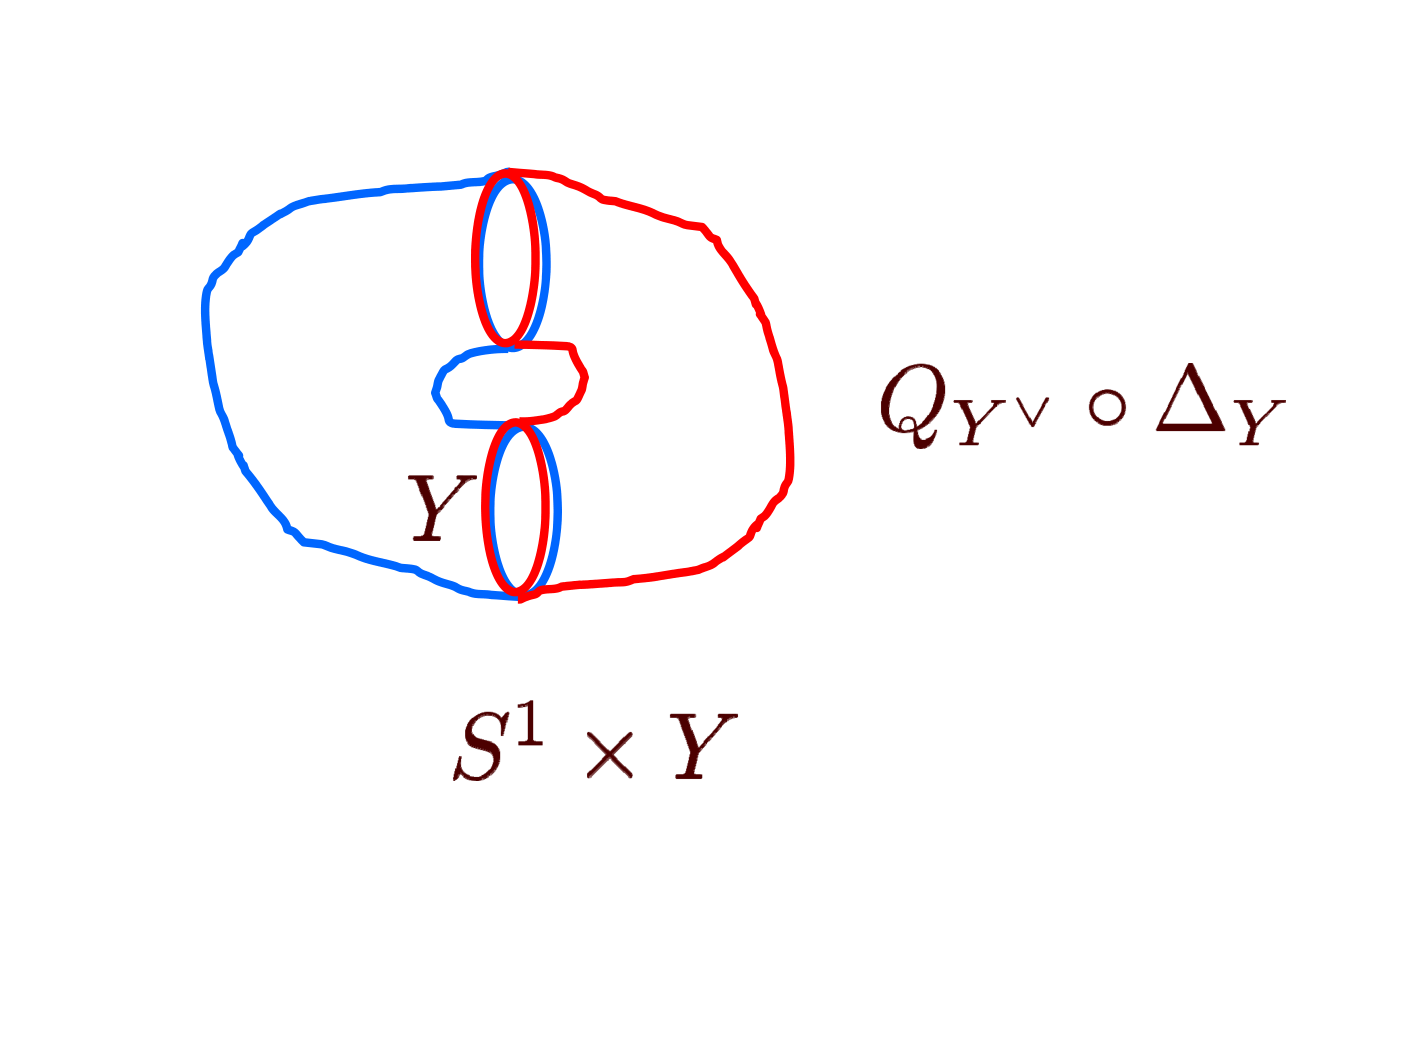
\includegraphics[width=0.45\textwidth]{figures/fig25.png}
  \caption{把 $Q_{Y^\vee}$ 与 $\Delta_Y$ 复合起来；在 $\mathbb{Z}_2$-分次情形它给出 $\mathcal{H}(Y)$ 的超维数，在非分次情形则给出 $\dim\mathcal{H}(Y)=Z(Y\times S^1)$。（原文 Fig.~25，第 153 页）}
  \label{fig:25}
\end{figure}

现在考虑图~\ref{fig:25} 中的图。一方面，这恰是配分函数 $Z(Y\times S^1)$。另一方面，线性映射 $\kappa\to\kappa$ 必须是复合 $Q_{Y^\vee}\Delta_Y$，或者等价地，$Q_Y\circ\Omega\circ\Delta_Y:\kappa\to\kappa$。由上面关于 $\Delta_Y(1)$ 的公式我们看到，$Z(Y\times S^1)$ 的值恰是维数 $\dim\mathcal{H}(Y)$，或者在 $\mathbb{Z}_2$-分次情形是超维数
\begin{equation}
  \operatorname{sdim}\mathcal{H}(Y)=\dim\mathcal{H}(Y)_0-\dim\mathcal{H}(Y)_1
  \tag{5.18}
  \label{eq:5.18}
\end{equation}

\textbf{评注}

\begin{enumerate}
  \item 注意若把范畴换成带 Riemann 结构的流形范畴，并在 $Y\times S^1$ 上取乘积 Riemann 结构，则
\begin{equation}
  Z(Y\times S^1)=\operatorname{Tr}e^{-\beta H}
  \tag{5.19}
  \label{eq:5.19}
\end{equation}
其中 $\beta$ 是圆的半径，$H$ 是 Hamilton 量。
% [Tutor Note: \eqref{eq:5.19} 与 \eqref{eq:5.18} 的对照是本节最易出错处：在 $\mathbb{Z}_2$-分次情形，能与 \eqref{eq:5.18} 相符的迹必须是超迹 $\operatorname{Tr}(-1)^F e^{-\beta H}$，而 \eqref{eq:5.19} 写的是普通迹——两者只在非分次情形一致。此外原文称 $\beta$ 为圆的半径；按 $Z=\operatorname{Tr}e^{-\beta H}$ 的标准推导，$\beta$ 实际是 $S^1$ 的周长（温度的倒数），若真的取半径为 $\beta$，指数上应出现 $2\pi\beta H$。两处均照原文转写，未作订正]
  \item 物理文献中有些重要的「拓扑场论」例子是违反这一条件的。一例是取非紧规范群的 Chern-Simons 理论。另一例是面积元为零的二维 Yang-Mills 理论。这些都是「部分定义」的拓扑场论：它们只在配边范畴中对象的一个子集上有定义。{\small\itshape ［原文标记：再说详细些。］}
% [原文待办标记（页边），原文 p.154：原文作 \ensuremath{\clubsuit}Say more. \ensuremath{\clubsuit}，作者自留的补充提示]
  \item 上面的 S-图论证指出了在对称幺半范畴中定义对偶对象（dual object）的路子。对偶对象 $x\in\operatorname{Obj}(C)$ 是指这样的对象：存在对象 $x^\vee\in\operatorname{Obj}(C)$ 以及态射 $\delta_x:1_C\to x\otimes x^\vee$ 与 $q_x:x^\vee\otimes x\to1_C$，使得
\begin{equation}
  x\xrightarrow{\iota_L(x)^{-1}}1_C\otimes x\xrightarrow{\delta_x\otimes1_x}x\otimes x^\vee\otimes x\xrightarrow{1_x\otimes q_x}x\otimes1_C\xrightarrow{\iota_R(x)}x
  \tag{5.20}
  \label{eq:5.20}
\end{equation}
并且（为简单起见，省略与张量单位相乘的同构）
\begin{equation}
  x^\vee\xrightarrow{1_{x^\vee}\otimes\delta_x}x^\vee\otimes x\otimes x^\vee\xrightarrow{q_x\otimes1_{x^\vee}}x^\vee
  \tag{5.21}
  \label{eq:5.21}
\end{equation}
都是恒等态射。
\end{enumerate}
% [Tutor Note: \eqref{eq:5.20}--\eqref{eq:5.21} 这两个复合等于恒等态射，就是张量范畴中的「蛇形（zig-zag）恒等式」，它们是把前面 S-图的拓扑事实转写成代数公理的结果。抄写时注意三处细节：单位同构记作 $\iota_L,\iota_R$（左、右单位同构）而非 $l,r$；$\delta_x$ 与 $q_x$ 的下标是对象 $x$ 而非流形 $Y$（与 \eqref{eq:5.11}--\eqref{eq:5.12} 的 $\Delta_Y,Q_Y$ 是同一构型的范畴化）；\eqref{eq:5.21} 中作者明言省略了与张量单位相乘的同构，故该链的两端只写到 $x^\vee$。术语取舍：「dual object」译作「对偶对象」、「dual pairing」译作「对偶配对」，「linear dual space」译作「线性对偶空间」，三者中文都用「对偶」以免与「自伴/共轭」混淆]

\begin{figure}[htbp]
  \centering
  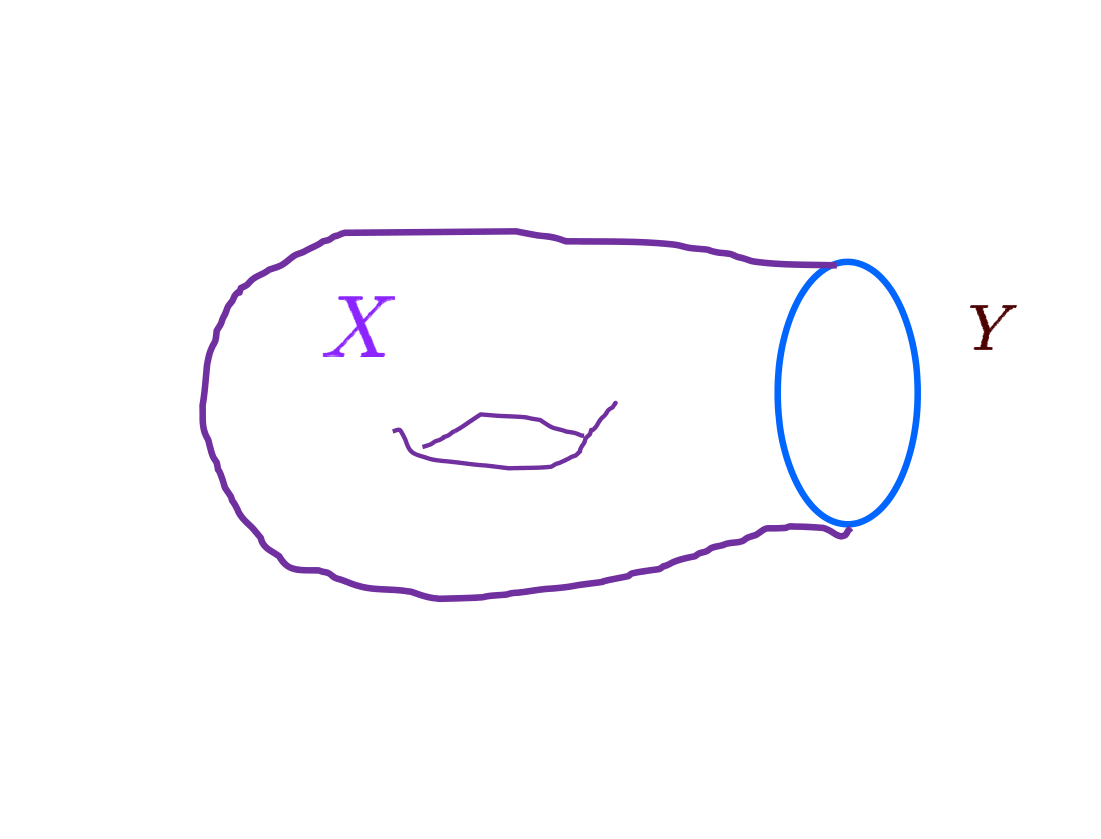
\includegraphics[width=0.50\textwidth]{figures/fig26.png}
  \caption{由从 $\emptyset$ 到 $Y$ 的一条配边所生成的一个态。（原文 Fig.~26，第 154 页）}
  \label{fig:26}
\end{figure}

\begin{figure}[htbp]
  \centering
  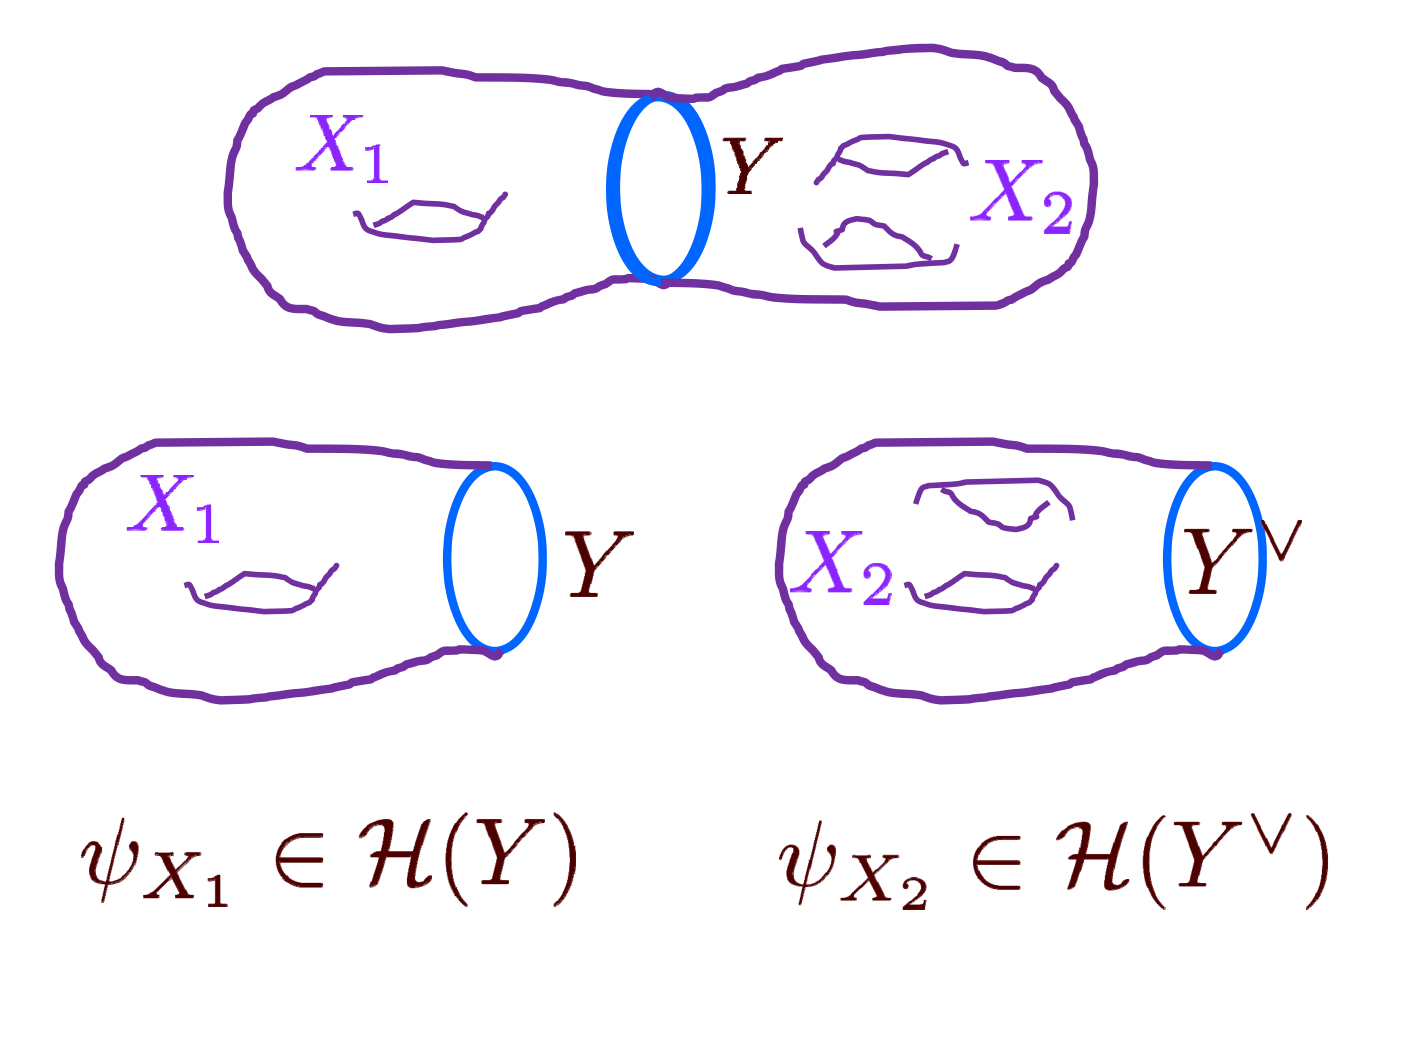
\includegraphics[width=0.50\textwidth]{figures/fig27.png}
  \caption{若闭流形 $X$ 沿一个余维一的子流形 $Y$ 切开，而 $Y$ 把 $X$ 分成两块 $X_1$ 与 $X_2$，则有两个相应的态 $\psi_{X_1}\in\mathcal{H}(Y)$ 与 $\psi_{X_2}\in\mathcal{H}(Y^\vee)$；配分函数 $Z(X)$ 的值可以看作这两个态用非退化配对 $Q_Y$ 所作的自然缩并。（原文 Fig.~27，第 155 页）}
  \label{fig:27}
\end{figure}

\medskip\noindent\textbf{练习}\quad\emph{映射柱与微分同胚群的特征标}

设 $f\in\operatorname{Diff}(Y)$，考虑映射柱 $M_f(Y)=([0,1]\times Y)/\!\sim$，其中我们把 $(0,y)$ 与 $(1,f(y))$ 等同起来。回忆 $\mathcal{H}(Y)$ 上有微分同胚群的表示 $\rho(f)$。

证明
\begin{equation}
  Z(M_f(Y))=\operatorname{Tr}_{\mathcal{H}(Y)}\rho(f)
  \tag{5.22}
  \label{eq:5.22}
\end{equation}
是微分同胚群的一个特征标。

事实上，$\rho(f)$ 只依赖于 $f$ 在映射类群（mapping class group）$\Gamma_Y$ 中的像：$\Gamma_Y$ 的定义如下——与恒等映射同痕（isotopic）的微分同胚构成全微分同胚群的一个正规子群 $\operatorname{Diff}_0(Y)$，而 $\Gamma_Y:=\operatorname{Diff}(Y)/\operatorname{Diff}_0(Y)$。{\small\itshape ［原文标记：详细解释 $\rho(f)$ 在 $f$ 的同痕下的独立性如何由公理推出。］}
% [原文待办标记（页边竖排），原文 p.155：原文作 \ensuremath{\clubsuit}Explain in detail how the independence of ρ(f) under isotopy of f follows from the axioms.\ensuremath{\clubsuit}，插在 "This is ... defined as follows" 之间]
% [Tutor Note: \eqref{eq:5.22} 是 \eqref{eq:5.18} 的「带扭转」版本：当 $f=Id$ 时 $M_f(Y)=Y\times S^1$，\eqref{eq:5.22} 退化为 $Z(Y\times S^1)=\operatorname{Tr}_{H(Y)}Id=\dim\mathcal{H}(Y)$，与 \eqref{eq:5.18} 一致（分次情形须改用超迹，参见 \eqref{eq:5.19} 的批注）。另外，作者在页边标记处想说的是：$\rho(f)$ 只依赖 $f$ 的同痕类，这一点的证明要用到「同痕可通过在 $[0,1]\times Y$ 上作微分同胚、把它在两端拉成恒等」这一事实；这正是把 \eqref{eq:5.22} 写成映射类群的特征标而非微分同胚群的特征标的依据]

\medskip\noindent\textbf{练习}\quad\emph{Hartle-Hawking 态与作为内积的配分函数}
% [原文标题误拼为 "Hartle-Hawking sates"，译文按 states 处理]

a.) 证明：任意配边 $X:\emptyset\to Y$ 都在空间 $\mathcal{H}(Y)$ 中定义一个\emph{态}。（见图~\ref{fig:26}。）拓扑场论的函子给出一个映射 $F(X):\kappa\to\mathcal{H}(Y)$，于是我们可以定义
\begin{equation}
  \psi_X:=F(X)(1)\in\mathcal{H}(Y)
  \tag{5.23}
  \label{eq:5.23}
\end{equation}

% =====================================================================
%  c19 —— 原文印刷页 156–164（PDF 第 157–165 页）
%  含：5.2.2 酉性、5.3 一维场论、5.4 二维拓扑场论、5.5 扩展拓扑场论、
%  5.6 三维拓扑场论、5.7 拓扑场论的若干原始文献；第 6 章（6.1–6.4）、
%  第 7 章（7.1、7.1.1）、第 8 章、第 9 章、第 10 章（10.1）开头；
%  插图 Fig. 28–31。
%  说明：原文第 5.3–5.7 小节在稿中大量只存提纲，译文照录其提纲文字。
% =====================================================================

这一简单的观察在物理中非常重要。

当然，态依赖于配边的（拓扑）细节。例如，任何带一个洞的 Riemann 面都定义了从圆周到零的配边，而这样的拓扑有很多。这是量子引力中「Hartle-Hawking」态这一概念的一个原始版本。它也与共形场论中的态／算符对应有关。

\quad b.) 证明：在带定向的配边范畴中，通过交换入边界与出边界（但不改变 $X$ 的定向），同一个流形定义了一个配边 $X^\vee: -Y\to\emptyset$，从而是 $\mathcal{H}(Y^\vee)$ 上的一个线性泛函。

\quad c.) 证明：把这个线性泛函作用于 $\Delta_Y(1)$，会还原出与 $X$ 相联系的 $\mathcal{H}(Y)$ 中的那个原向量。

\quad d.) 证明：若闭流形 $X$ 沿带定向流形 $Y$ 切开而得到 $X_1$ 与 $X_2$，则 $Z(X)$ 可以解释为态 $\psi_{X_1}\in\mathcal{H}(Y)$ 与 $\psi_{X_2}^\vee\in\mathcal{H}(Y^\vee)$ 的一种缩并：
\begin{equation}
  Z(X)=\langle \psi_{X_2}^\vee,\psi_{X_1}\rangle
  \tag{5.24}
  \label{eq:5.24}
\end{equation}
见图~\ref{fig:27}。

\subsubsection{酉性} % 原文: 5.2.2 Unitarity

在酉理论中——当然也在量子力学的公理中——人们要求态空间是复 Hilbert 空间，而配边 $X$ 所对应的 $F(X)$ 应当是酉算符。

现在，一般地，复向量空间 $V$ 上的半双线性形式（sesquilinear form）是一个线性映射 $V\to\bar V^\vee$。因此，在酉理论中改变 $Y$ 的定向相当于对 Hilbert 空间取复共轭：
\begin{equation}
  \mathcal{H}(Y^\vee)\cong\bar{\mathcal{H}}(Y)
  \tag{5.25}
  \label{eq:5.25}
\end{equation}

此外，在物理的酉理论中，$Q_Y$ 上还带有一个正性条件。若 $X: Y_1\to Y_2$ 是配边，那么改变 $X$ 的定向并取对偶，我们便得到配边
\begin{equation}
  \bar X^\vee: Y_2\to Y_1
  \tag{5.26}
  \label{eq:5.26}
\end{equation}
自然地再补上一个条件：
\begin{equation}
  F(\bar X^\vee)=F(X)^\dagger
  \tag{5.27}
  \label{eq:5.27}
\end{equation}
特别地，对闭流形而言，改变流形的定向会使不变量 $Z(X)$ 取复共轭。
% [Tutor Note: (5.26) 的记号 $\bar X^\vee$ 里叠了两个操作，极易读漏其一：上划线是「取复共轭」，即反转 $X$ 的定向；$\vee$ 是「取对偶」，即交换入、出边界。$X:Y_1\to Y_2$ 经这两步叠加才变成 $Y_2\to Y_1$。(5.27) 断言这一复合恰等于 $F(X)$ 的 Hermite 共轭，所以既不能把 $\bar X^\vee$ 只读成「$X$ 的共轭」、也不能只读成「$X$ 的对偶」；核对时请与 (5.25) 对照：那里「变定向 $\Rightarrow$ 复共轭」用的是同一个 $\bar{\ }$，若此处误写为 $\bar X$（不取对偶），(5.27) 两边的边界就不匹配了]

\subsection{一维场论} % 原文: 5.3 One Dimensional Field Theories

考虑带定向的情形。此时 $\mathrm{Bord}^{\mathrm{SO}}_{\langle 0,1\rangle}$ 中的对象是点 $\mathrm{pt}_\pm$（分别带 $+$ 定向与 $-$ 定向）的不交并。

以对称幺半范畴（symmetric monoidal category）$C$ 为值的拓扑场论给出两个对象 $y_\pm=F(\mathrm{pt}_\pm)$，以及如上所述的数据 $\delta$ 与 $q$。一般的对象是 $n_\pm$ 个 $\mathrm{pt}_\pm$ 型点的不交并。这个流形的微分同胚群恰为 $S_{n_+}\times S_{n_-}$，它自然地作用在「态空间」$y_+^{\otimes n_+}\otimes y_-^{\otimes n_-}$ 上。

专门取到 $\mathrm{VECT}_\kappa$，我们便得到一对有限维向量空间 $V_\pm$，连同上面提到的数据：一个非退化配对 $Q: V_+\otimes V_-\to\kappa$，以及「逆」$\Delta: \kappa\to V_+\otimes V_-$。如前所述，这些数据构成 $V_-=V_+^\vee$ 的对偶数据。

这类拓扑场论的一个很好的物理来源，是考虑紧辛流形（compact symplectic manifold）$(M,\omega)$ 的量子化。

一个值得记住的、有用的具体例子是 $M=S^2$，其辛形式为
\begin{equation}
  \omega=\frac{1}{2\hbar}\sin\theta\, d\theta\, d\phi
  \tag{5.28}
  \label{eq:5.28}
\end{equation}
这里 $\hbar$ 是该形式的某个无量纲归一化常数。

在路径积分的 Hamilton 表述中，我们考虑相空间 $M$ 中的路径。我们构造如下形式的路径积分
\begin{equation}
  \int_{\mathcal{P}}[d\gamma]\,\exp[\mathrm{i}S]
  \tag{5.29}
  \label{eq:5.29}
\end{equation}
其中 $\mathcal{P}$ 是 $M$ 中路径构成的空间，$[d\gamma]$ 是由辛形式在路径空间上诱导出的测度，$S$ 是作用量。要使这个表达式有意义，有许多问题需要解决。我们在这里只触及其中几点。

若辛形式 $\omega$ 整体恰当（globally exact），则可写 $\omega=d\lambda$，其中用局部 Darboux 坐标表示
\begin{equation}
  \lambda=\frac{1}{\hbar}pdq
  \tag{5.30}
  \label{eq:5.30}
\end{equation}
一个很好的例子是 $M=T^*X$（$X$ 为某流形）。注意，与这个作用量原理
\begin{equation}
  S[\gamma]=\frac{1}{\hbar}\int_\gamma pdq
  \tag{5.31}
  \label{eq:5.31}
\end{equation}
相联系的 Hamilton 量为零。

但若 $\omega$ 不是恰当的，又当如何？（例如上面 $M=S^2$ 的例子。）让我们先假设 $M$ 是单连通的。此时若 $\gamma$ 是闭路径，我们可以试着这样定义作用量：选取一个圆盘 $\Sigma\subset M$ 使 $\partial\Sigma=\gamma$，然后取
\begin{equation}
  S_\Sigma[\gamma]:=\int_\Sigma \omega
  \tag{5.32}
  \label{eq:5.32}
\end{equation}
若 $\omega$ 恰当，这就回到先前的定义。

现在问题来了：以 $\gamma$ 为边界的圆盘可以不止一个。若 $\Sigma_1,\Sigma_2$ 都以 $\gamma$ 为边界，则 $\Sigma_{12}:=\Sigma_1\cup_\gamma\Sigma_2^\vee$ 是一个 $2$-维闭链，而作用量的不确定性为
\begin{equation}
  S_{\Sigma_1}[\gamma]-S_{\Sigma_2}[\gamma]=\int_{\Sigma_{12}}\omega
  \tag{5.33}
  \label{eq:5.33}
\end{equation}
所以作用量并非良定义。然而，量子路径积分所需的其实只是权重
\begin{equation}
  \exp[\mathrm{i}S]=\exp\Big[\mathrm{i}\int_\Sigma \omega\Big]
  \tag{5.34}
  \label{eq:5.34}
\end{equation}
应当是良定义的。指数化作用量的不确定性是：
\begin{equation}
  \exp[\mathrm{i}S_1]/\exp[\mathrm{i}S_2]=\exp\Big[\mathrm{i}\int_{\Sigma_{12}}\omega\Big]
  \tag{5.35}
  \label{eq:5.35}
\end{equation}
只要 $\omega$ 的周期是 $2\pi$ 的整数倍，左端就等于一，路径积分中也就有了无歧义的权重。请注意，这实际上把「$1/\hbar$」量子化为整数。
% [Tutor Note: 这里「把 $1/\hbar$ 量子化为整数」一句容易读错归一处。关键在 (5.28)：作者一开始就把 $1/\hbar$ 吸收进了辛形式本身（对比 (5.30) 中 $\lambda=pdq/\hbar$），所以 (5.33)–(5.35) 的整性条件是 $\int_{\Sigma_{12}}\omega\in 2\pi\mathbb{Z}$，它约束的是 $\omega$ 里的 $1/\hbar$；若换用「$\omega$ 不含 $1/\hbar$」的约定，同一条件就要改写成对 $\hbar$ 的整性要求。核对 (5.32) 与 (5.31) 是否相容时，务必先确认 $\omega$ 的这一归一化，否则会差一个 $\hbar$ 的幂]

现在，假设 $\gamma$ 不是闭路径。让我们考虑路径空间
\begin{equation}
  \mathcal{P}=\{\gamma:[0,1]\to M\,|\,\gamma(0)=x_0\quad\&\quad\gamma(1)=x_1\}
  \tag{5.36}
  \label{eq:5.36}
\end{equation}
（我们假设 $x_0,x_1$ 位于 $M$ 的同一个道路连通分支中。）在 $\mathcal{P}$ 中选取一条基点路径 $\gamma_0$。那么任何与 $\gamma_0$ 同伦的路径 $\gamma$ 都会使得 $\gamma_0^{-1}*\gamma$ 围出一个圆盘 $\Sigma$。我们随即用这些数据把作用量定义为
\begin{equation}
  S_{\gamma_0,\Sigma}[\gamma]:=\int_\Sigma \omega.
  \tag{5.37}
  \label{eq:5.37}
\end{equation}
对固定的基点路径，只要 $\omega$ 的周期落在 $2\pi\mathbb{Z}$ 中，指数化作用量就与 $\Sigma$ 的选取无关。若把基点路径 $\gamma_0$ 换成同一同伦类中的另一条，作用量只会差一个常数；而实际上，在如上把 $\omega$ 量子化之后，这一选取在指数化作用量中也同样无关紧要。
% [Tutor Note: (5.37) 从「$\gamma$ 与 $\gamma_0$ 同伦」直接跳到「作用量只差常数」，中间被省略的一步是：换基点路径 $\gamma_0\to\gamma_0'$ 时 $\gamma_0'^{-1}*\gamma_0$ 是一条闭道路，于是作用量之差等于 $\omega$ 在该闭道路所围闭链上的周期，而由前面「周期属于 $2\pi\mathbb{Z}$」的假设，指数化之后此差别为 1。也正因这一步只用到了同伦类的信息，(5.37) 对「不与 $\gamma_0$ 同伦的路径」根本没有定义——这正是下一段要处理的问题]

若 $M$ 不是单连通的，就需要额外的考虑：此时即使 $x_0,x_1$ 在 $M$ 的同一道路连通分支中，$\mathcal{P}$ 里仍会有不与 $\gamma_0$ 同处一个道路连通分支的路径。处理这一点的一个办法是在万有覆叠 $\widetilde{M}$ 上工作。最好的做法则是把理论耦合到 $M$ 上的一个平坦联络，以便追踪基本群。
{\small\itshape ［原文标记：EXPLAIN MORE!（要再解释清楚些！）］}
% [原文待办标记，原文 p.158；紧接在「耦合平坦联络以追踪基本群」一句之后，作者自注此处需补充说明]

上面量子化的一个重要特例，是紧单 Lie 群由整权 $\lambda\in\mathfrak{g}^*$ 所定义的余伴随轨道（coadjoint orbit）。这里有一个自然的、整量子化的辛形式，即 Kirillov-Kostant 辛形式；量子化之后给出一个表示，其支配权（dominant weight）向量是 $\lambda$ 的某个适当的 Weyl 旋转。沿着这条思路走下去，可以得到 Borel-Weil-Bott 定理的路径积分解释。在
{\small\itshape ［原文标记：Do it later?（这个以后再做？）］}
% [原文待办标记，原文 p.158；该标记插在句子中间（"In \ensuremath{\clubsuit}...\ensuremath{\clubsuit} the topological field theory"），译文照其位置保留在「在……拓扑场论中」之间]
该拓扑场论中，空间 $V_+$ 是支配权为 $\lambda$ 的表示，空间 $V_-$ 是反支配权为 $-\lambda$ 的共轭表示。对偶数据 $Q$ 是表示与其共轭表示构成单态（singlet）的标准配对，而 $\Delta$ 则是把单态嵌入 $R\otimes R^\vee$ 的映射。
% [Tutor Note: 这一段把 Kirillov-Kostant 形式「可量子化」与「给出不可约表示」两步一笔带过。被省略的是 Borel-Weil-Bott 定理的内容：$\lambda$ 必须是整权（否则该辛形式不是整的、预量子线丛不存在），并且要把 $\lambda$ 用 Weyl 群移到支配 Weyl 腔才对应不可约表示的最高权；非支配的 $\lambda$ 给出的是同一表示的「Weyl 反射」版本。这也是原文为何写 "a suitable Weyl rotation of $\lambda$"。细节可查 Kirillov《Lectures on the Orbit Method》或 Bott 的原始论文]

{\small\itshape ［原文标记：SHOULD ADD MATERIAL ON STOLZ-TEICHNER VIEWPOINT HERE（此处应补入 Stolz-Teichner 观点的材料）］}
% [原文待办标记，原文 p.158；原稿以两行 $*$ 号分隔线上下框住这段全大写文字]

\subsection{二维拓扑场论} % 原文: 5.4 Two-Dimensional Topological Field Theories

需要说明：
\begin{enumerate}
  \item 缝合定理（sewing theorem）与交换 Frobenius 代数；
  \item 如何计算全部振幅；
  \item 半单情形：时空解释；
  \item 开-闭定理（open-closed theorem），以及把边界条件看作某个范畴中的对象；
  \item 半单情形：时空解释；
  \item 如何使理论等变（equivariant）。
\end{enumerate}
以上全部内容：详尽讨论见 GMP2015: [47]。
% 原文此处列表编号为 1.–6.，其中第 1、2 项在印刷页 158，第 3–6 项与末行全大写提示在印刷页 159

\subsection{扩展拓扑场论} % 原文: 5.5 Extended Topological Field Theories

{\small\itshape ［原文标记：CAN ALREADY ILLUSTRATE THE IDEA WITH 2D THEORIES / Follow discussion in [47].（用二维理论就足以说明这一想法。按 [47] 中的讨论进行。）］}
% [原文待办标记，原文 p.159；原稿以两行 $*$ 号分隔线把这两行全大写／普通字体的提示框住]

\subsection{三维拓扑场论} % 原文: 5.6 Three-Dimensional Topological Field Theories

\begin{enumerate}
  \item[5.] 张量范畴（tensor category）。
  \item[6.] 模张量范畴（modular tensor category）。定理：MTC 给出三维酉 TFT。
\end{enumerate}
这一点或许应当放到我们回到三维非阿贝尔 Chern-Simons 之后再讲？
% 原文此处两项的编号沿用前一小节的列表，分别为 5. 与 6.（第 6 项缩进一级）

\subsection{拓扑场论的若干原始文献} % 原文: 5.7 Some Source Material For Topological Field Theories

关于拓扑场论有极其庞大的文献。早期的一篇关键论文是

\qquad 1.\ M.F. Atiyah, ``Topological quantum field theories.'' Inst. Hautes Etudes Sci. Publ. Math. No. 68 (1988), 175-186 (1989).

这篇论文受到 Witten 的工作以及 Graeme Segal 对共形场论的公理化表述的启发，后者现在可见于：

\qquad 2.\ G. Segal, ``The Definition Of Conformal Field Theory,'' 载于 \emph{Topology, Geometry and Quantum Field Theory: Proceedings of the 2002 Oxford Symposium in Honour of the 60th Birthday of Graeme Segal}。

若想要一份更多从物理学家视角写成的导引，请看

\qquad D. Birmingham, M. Blau, M. Rakowski,m and G. Thompson, ``Topological Field Theory,'' Phys.\ Rept.\ 209 (1991) 129-340

我们还参考了讲义

\qquad 3.\ Segal, Stanford notes, \texttt{http://www.cgtp.duke.edu/ITP99/segal/}

以及这篇综述性文章：

\qquad 4.\ G. Segal and G. Moore, ``D-branes and K-theory in 2D topological field theory'' hep-th/0609042。另见 P. Aspinwall 等，\emph{Mirror Symmetry II}, Clay Mathematics Institute Monograph 一书的第 2 章。

关于拓扑场论的一般情形，极为细致审慎的讨论见

\qquad 5.\ V.G. Turaev, \emph{Quantum Invariants Of Knots And 3-Manifolds}, De Gruyter, 2nd edition 2010.

$d=3$ 的 TQFT 与模张量范畴这一特例，最早得到详细描述是在

\qquad G. Moore and N. Seiberg, ``Lectures on RCFT,'' 载于 \emph{Superstrings '89}, World Scientific, pp.\ 1-129.

其后的专著

\qquad Bakalov and Kirillov

给出了更细致的处理。

我们用到了 Dan Freed 那份非常好的讲义中的一些材料：

\qquad 10.\ D. Freed, ``Bordism Old And New,'' \texttt{https://www.ma.utexas.edu/users/dafr/M392C-2012/index.html}

关于高阶范畴论与局域性的近期进展，请看

\qquad 11.\ A. Kapustin, ``Topological Field Theory, Higher Categories, and Their Applications,'' arXiv:1004.2307 [math.QA]

\qquad 12.\ J. Lurie, ``On the classification of topological field theories,'' arXiv:0905.0465 [math.AT]

\qquad 13.\ D. Freed, ``The cobordism hypothesis'' BAMS

\qquad 14.\ D. Freed, ``Remarks On Chern-Simons Theory,'' Bull.\ AMS, 46 (2009), pp.\ 221-254
% 原文此处的文献编号从 5. 直接跳到 10.（作者原稿的编号不连续），译文照原编号保留

\section{用 RCFT 计算非阿贝尔 Chern-Simons 关联函数} % 原文: 6. Computing Nonabelian Chern-Simons Correlators Using RCFT

\begin{keytakeaways}
  \item 核心事实：在手征代数的不可约表示所对应的典范基下写出的模变换 $S$ 矩阵，等于 $S^3$ 中两条相互链接的圆上、分别带有对应表示的线缺陷时路径积分的值。原稿在图~\ref{fig:10} 中「从实验上」观察到了这一点，本节说明它实际上相当普遍。
  \item 论证只依赖两条关键事实：(i) 两个 $D^2\times S^1$ 柄体沿边界粘合，若按 $D^2$ 粘成球面的方式粘，得到 $S^2\times S^1$；若用交换两个圆周期的 $S$ 变换粘，得到 $S^3$。(ii) 沿柄体核心插入线缺陷会在 $\mathcal{H}(T^2)$ 中产生态。
  \item 粘合前必须对两个态之一作用 $S$；配合 $\mathcal{H}(T^2)$ 上使 $\chi_i$ 正交归一的双线性形式，即可读出 $S$ 矩阵与链接圆上路径积分的相等关系。
  \item 对 Verlinde 公式，原稿只给了一条「奥林匹亚式」的捷径：按 Moore-Seiberg《Lectures on RCFT》习题 7.13 走一遍。
\end{keytakeaways}

\subsection{编织矩阵与融合矩阵的三维解释} % 原文: 6.1 3D Interpretation Of Braiding And Fusing Matrices
% 原文此小节只有标题，没有正文（原稿在此仅留标题，内容显然尚待补写）

\subsection{手术操作} % 原文: 6.2 Surgery Manipulations

\subsubsection*{模 $S$ 矩阵的三维解释}
% 原文此行是一个无编号的下划线小标题（位于 6.2 之下、6.3 之前）；因其无编号，用带星号的标题复刻，不参与自动编号

我们在图~\ref{fig:10} 中从实验上观察到：模变换 $S$ 矩阵——在以对应于手征代数不可约表示的典范基写出时——等于 $S^3$ 中带有相应表示的线缺陷的两条链接圆上路径积分的值。事实上，这个关系相当普遍，我们现在就来解释。

我们需要两条关键事实：

\begin{enumerate}
  \item 取两份柄体（handlebody）$D^2\times S^1$。其边界是 $S^1\times S^1$，其中第一个 $S^1$ 因子是 $D^2$ 的边界。若把这两个柄体粘在一起，使两份 $D^2$ 粘成一个球面，则所得的闭 $3$-流形是 $S^2\times S^1$。另一方面，若用一个交换两个圆周期的 $S$ 变换来粘这两个 $T^2$ 因子，则所得的 $3$-流形是 $S^3$。看清这一点有一个相当快捷的办法：注意到所得的 $3$-流形是单连通的，因为环面中的 $a,b$ 两个圈可以在其中一个或另一个柄体里连续收缩为一点。然后引用 Poincaré 猜想即可。一个更初等的证明是……
  {\small\itshape ［原文标记：GIVE A PROOF THAT DOES NOT RELY ON POINCARE（给出一个不依赖 Poincaré 猜想的证明）］}
  % [原文待办标记，原文 p.160；紧接在「一个更初等的证明是……」之后，作者自注此处需要一个不依赖 Poincaré 猜想的证明]

  \item 现在考虑沿上述两个柄体各自的核心插入线缺陷的路径积分，一个对应表示 $i$、一个对应表示 $j$。它们在该 $\mathcal{H}(T^2)$ 中产生相应的态 $\chi_i,\chi_j$。这个空间上有一个双线性形式，使得这些态在其中正交归一。另一方面，当我们用模变换来粘合边界时，必须在粘合前对两个态之一作用 $S$。一般结果便随之得到。
  {\small\itshape ［原文标记：NEED TO EXPLAIN!!（此处需要解释！！）］}
  % [原文待办标记，原文 p.160；针对「粘合前须对两态之一作用 $S$」这一步]
\end{enumerate}

{\small\itshape ［原文标记：EXPLAIN THIS BETTER.（这一点要解释得更好。）］}
% [原文待办标记，原文 p.161；位于「一般结果便随之得到」之后]

Verlinde 公式的奥林匹亚式证明：按 Moore-Seiberg《Lectures on RCFT》习题 7.13 做。
% [Tutor Note: 这里的「奥林匹亚式证明」指一跳到底、只留关键动作的证明。习题 7.13 的实际内容是用 (i) 中两种粘合方式给出的态的内积、以及 (ii) 中 $S$ 对其中一个态的作用，把 Verlinde 公式 $N_{ij}^{\ \ k}=\sum_n S_{in}S_{jn}S_{kn}^*/S_{0n}$ 化成一次矩阵乘法；缺的中间步骤是「粘贴两次得到 $S^2$ 的矩阵元关系」。若手头没有 Moore-Seiberg 讲义，可对照 Bakalov-Kirillov 第 3 章中同一结论的推导]

\subsection{Jones 多项式与 WRT 不变量} % 原文: 6.3 The Jones polynomial and WRT Invariants

\begin{enumerate}
  \item 纽结不变量与 Reidemeister 移动；
  \item skein 关系；
  \item Jones 多项式；
  \item 推广：按 Witten 的着色 Jones 多项式；
  \item 路径积分：WRT 不变量；
  \item 用编织、融合与 $S$ 矩阵的数据进行计算。
\end{enumerate}

\subsection{超越纽结多项式：范畴化与纽结同调的想法} % 原文: 6.4 Beyond knot polynomials: The idea of categorification and Knot homology.

\section{有限群 Chern-Simons 理论} % 原文: 7. Finite Group Chern-Simons Theory

\begin{keytakeaways}
  \item 三维 Chern-Simons 理论对\emph{任意}紧 Lie 群都可以定义（前文讨论的多是单连通或单的情形，这里强调的是「任意」）；一般紧 Lie 群的结构见附录 J.1。
  \item 当规范群取有限群 $G$ 时，理论由群上同调（group cohomology）刻画，其分类空间 $BG$ 的上同调给出理论的数据。
  \item 「能级」（level）在这一情形下的自然归宿是 $H^4(BG;\mathbb{Z})$；相应文献为 Dijkgraaf-Witten 与 Freed（原文此处拼作 ``Dijgraaf''）。
\end{keytakeaways}

\subsection{一般紧群 $G$} % 原文: 7.1 The General Compact Group G

三维 Chern-Simons 理论可以对任意紧 Lie 群定义。关于一般紧 Lie 群长什么样，可参见附录 J.1。

\subsubsection{规范群为有限群时的 Chern-Simons 理论} % 原文: 7.1.1 Chern-Simons Theory When The Gauge Group Is A Finite Group

群上同调。

群上同调与 $BG$。

能级的自然归宿是 $H^4(BG;\mathbb{Z})$。

引用：Dijgraaf-Witten。Freed。
% 以上四行在原稿中即为提纲式短语（其中 "Dijgraaf" 系原稿拼法，通常拼作 Dijkgraaf），译文照录

\section{$p$-形式推广与微分上同调} % 原文: 8. p-form Generalizations And Differential Cohomology

\begin{keytakeaways}
  \item 本节只留下提纲：微分上同调（differential cohomology）的回顾，按 FK 讲义中的相应章节进行。
  \item 需要强调的要点是：阿贝尔 Chern-Simons 作用量不过是 Cheeger-Simons 的「相乘并积分」双线性形式的一次二次加细（quadratic refinement）。
  \item 本节在本片段中只有这两条提纲、没有可转写的公式，故原稿把展开留给了 FK 讲义。
\end{keytakeaways}

微分上同调的回顾：按 FK 讲义中的相应章节进行。

强调：阿贝尔 CS 作用量不过是 Cheeger-Simons「相乘并积分」双线性形式的一次二次加细。

\section{关于拓扑场论的更多内容} % 原文: 9. More About Topological Field Theories

\begin{keytakeaways}
  \item 本节（原稿仅存提纲）指出两个密切相关的话题：可逆拓扑场论（invertible topological field theory）与反常抵消（anomaly cancellation）。
  \item 可逆拓扑场论、配边理论与 SPT 相：原稿把这三者并列提出，作为与反常抵消相关的同一组话题。
  \item 原稿未展开细节，只留下标题性提示，故本节无可转写的推导。
\end{keytakeaways}

可逆拓扑场论与反常抵消。

可逆拓扑场论、配边理论以及 SPT 相。

\section{任意子、非阿贝尔任意子与量子计算} % 原文: 10. Anyons, nonabelions, and quantum computation

\begin{keytakeaways}
  \item 带电粒子被限制在二维空间中时，只有路径的拓扑才决定波函数相位的改变；把一对全同的 $(q,\Phi)$ 束缚态交换，所得相位可以解释为统计相位，而且它可以是\emph{任意}相位——这类粒子称为任意子（anyon）。
  \item 超导体提供了把磁通当作 $2+1$ 维「粒子」的现实机制：$U(1)$ 规范对称性被 Cooper 对的真空期望值自发破缺，磁通管是光子无质量的正常相区域，故磁通无法散开。
  \item 电荷 $q$ 与磁通 $\Phi$ 组成的束缚态 $(q,\Phi)$ 是 dyon 的 $2+1$ 维类比；两个全同束缚态交换给出的统计相位 $\exp[\mathrm{i}q\Phi/\hbar]$ 可以取\emph{任意}值。
  \item 自旋-统计关系：$2+1$ 维中角动量只有一个生成元 $J=J_{12}$，取 $\vec a=\vec R$ 代入 \eqref{eq:10.4} 即得 $\exp[2\pi\mathrm{i}J/\hbar]=\exp[\mathrm{i}q\Phi/\hbar]$，于是自旋与统计相位是同一件事。
\end{keytakeaways}

\subsection{2+1 维中的任意子} % 原文: 10.1 Anyons in 2+1 dimensions

现在让我们考虑：当带电粒子被限制在二维空间中生活时，会发生什么。参见
\begin{enumerate}
  \item \texttt{http://en.wikipedia.org/wiki/2DEG}
  \item S. Girvin, ``The Quantum Hall Effect: Novel Excitations and Broken Symmetries,'' arXiv:cond-mat/9907002
\end{enumerate}
以了解一些逼近这一理想情形的实验实现。
% 原文「See 1. ... 2. ... for a description of ...」是一个被列表打断的句子，此处照原结构译出

现在，如果我们的平面上还贯穿有细螺线管、其磁通量为 $\Phi$，那就很有意思了。我们可以设想这样一种情形：磁通无法散开，因而它们在 $2+1$ 维中也表现得像粒子。超导体就是这种情况如何发生的一个很好的例子。理解超导性的一个好方式，是把它看作一种电磁理论，其中 $U(1)$ 规范对称性被代表 Cooper 对的、电荷为二（charge two）的场的真空期望值自发破缺。磁通管是正常相的区域，其中光子无质量。超导体则是光子获得质量的区域。磁通无法散开。

现在设想——出于某种尚未指明的机制——一个电荷为 $q$ 的粒子束缚到这样一个螺线管粒子上。我们把该束缚态记为 $(q,\Phi)$。这些 dyon（双荷子）的 $2+1$ 维类比具有一些非常奇特的性质。

\begin{figure}[htbp]
  \centering
  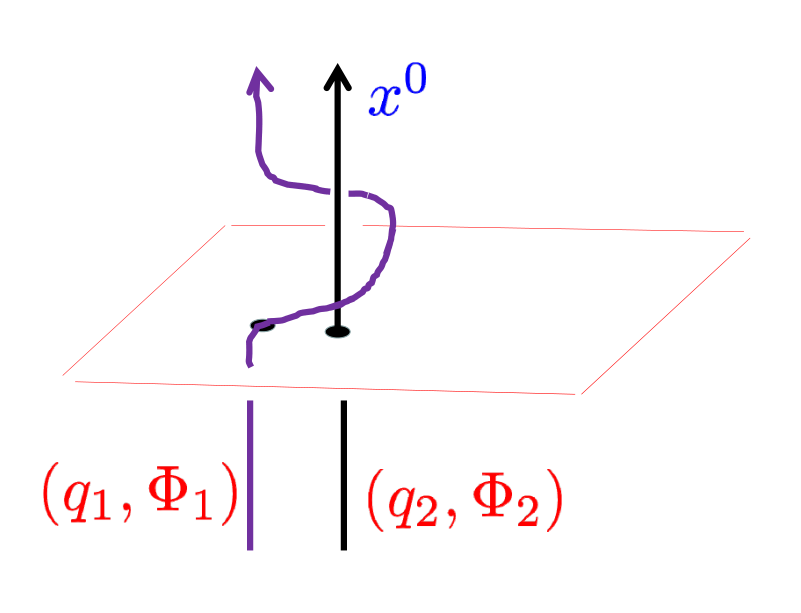
\includegraphics[width=0.6\textwidth]{figures/fig28.png}
  \caption{束缚态 $(q_1,\Phi_1)$ 极缓慢地沿逆时针方向绕过束缚态 $(q_2,\Phi_2)$。在计算波函数的相位变化时，只有路径的拓扑才有意义。不要把竖直方向与 $z$ 轴混淆：这里的竖直方向表示时间方向。（原文 Fig.~28，第 162 页）}
  \label{fig:28}
\end{figure}

让我们把粒子 $(q_1,\Phi_1)$ 极缓慢地绕过粒子 $(q_2,\Phi_2)$，如图~\ref{fig:28} 所示。应用公式 (??)，波函数获得相位 $\exp[\frac{\mathrm{i}}{\hbar c}(q_2\Phi_1)]$。注意这并不依赖轨迹的精确形状，只要求一个粒子绕着另一个转了一圈。与此同时，还有另一份相位变化，因为粒子 $(q_2,\Phi_1)$ 绕过了磁通 $\Phi_1$。事实上我们可以把图~\ref{fig:28} 形变成图~\ref{fig:29}。于是合起来，
% [Tutor Note: 原文此处和被引的「一般公式」都写作 "(??)"——作者源文件里这一交叉引用没有解析出来（应指后文 (10.2)–(10.4) 所在的那条一般公式，讲电荷绕磁通一周的 Aharonov-Bohm 相位）。这是原文自身的残缺，译文保留 "(??)" 以示未作补全]

\begin{figure}[htbp]
  \centering
  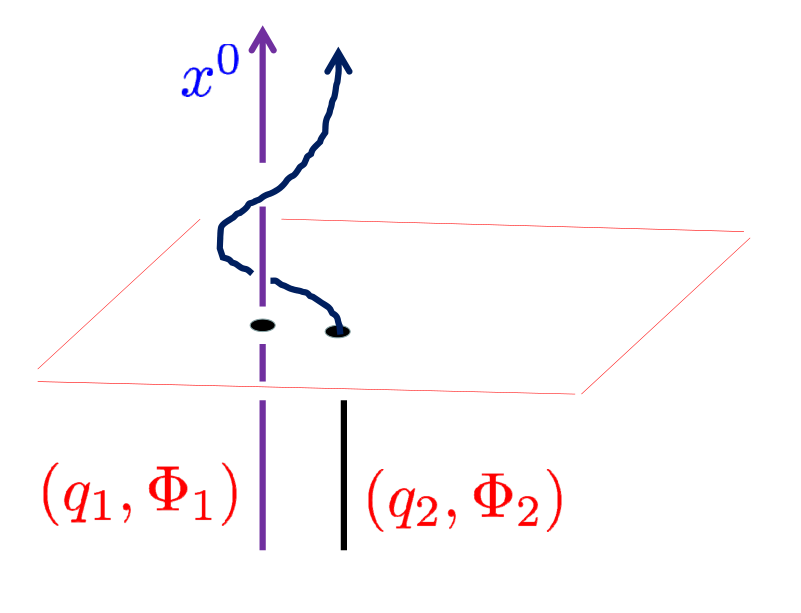
\includegraphics[width=0.6\textwidth]{figures/fig29.png}
  \caption{把 Figure~7 中的路径作拓扑等价的重新表述。由此可以清楚看出：束缚态 $(q_2,\Phi_2)$ 也沿逆时针方向绕 $(q_1,\Phi_1)$ 运动。（原文 Fig.~29，第 163 页）}
  \label{fig:29}
\end{figure}
% 原文疑似笔误：图注中的 "the path in Figure 7" 应为 "Figure 28"（本图的形变对象正是 Figure 28 中的路径）；照原文转写，未改

这对粒子的波函数改变为
\begin{equation}
  \exp\Big[\frac{\mathrm{i}}{\hbar}(q_2\Phi_1+q_2\Phi_2)\Big]
  \tag{10.1}
  \label{eq:10.1}
\end{equation}
% [Tutor Note: 原文 (10.1) 的第二项写作 $q_2\Phi_2$。按上下文（粒子 1 绕粒子 2 走、粒子 2 绕磁通 $\Phi_1$ 走，两份相位应分别为 $q_2\Phi_1$ 与 $q_1\Phi_2$），第二项似应为 $q_1\Phi_2$。此处照原式转写、未作改动，引用时请留意]

\begin{figure}[htbp]
  \centering
  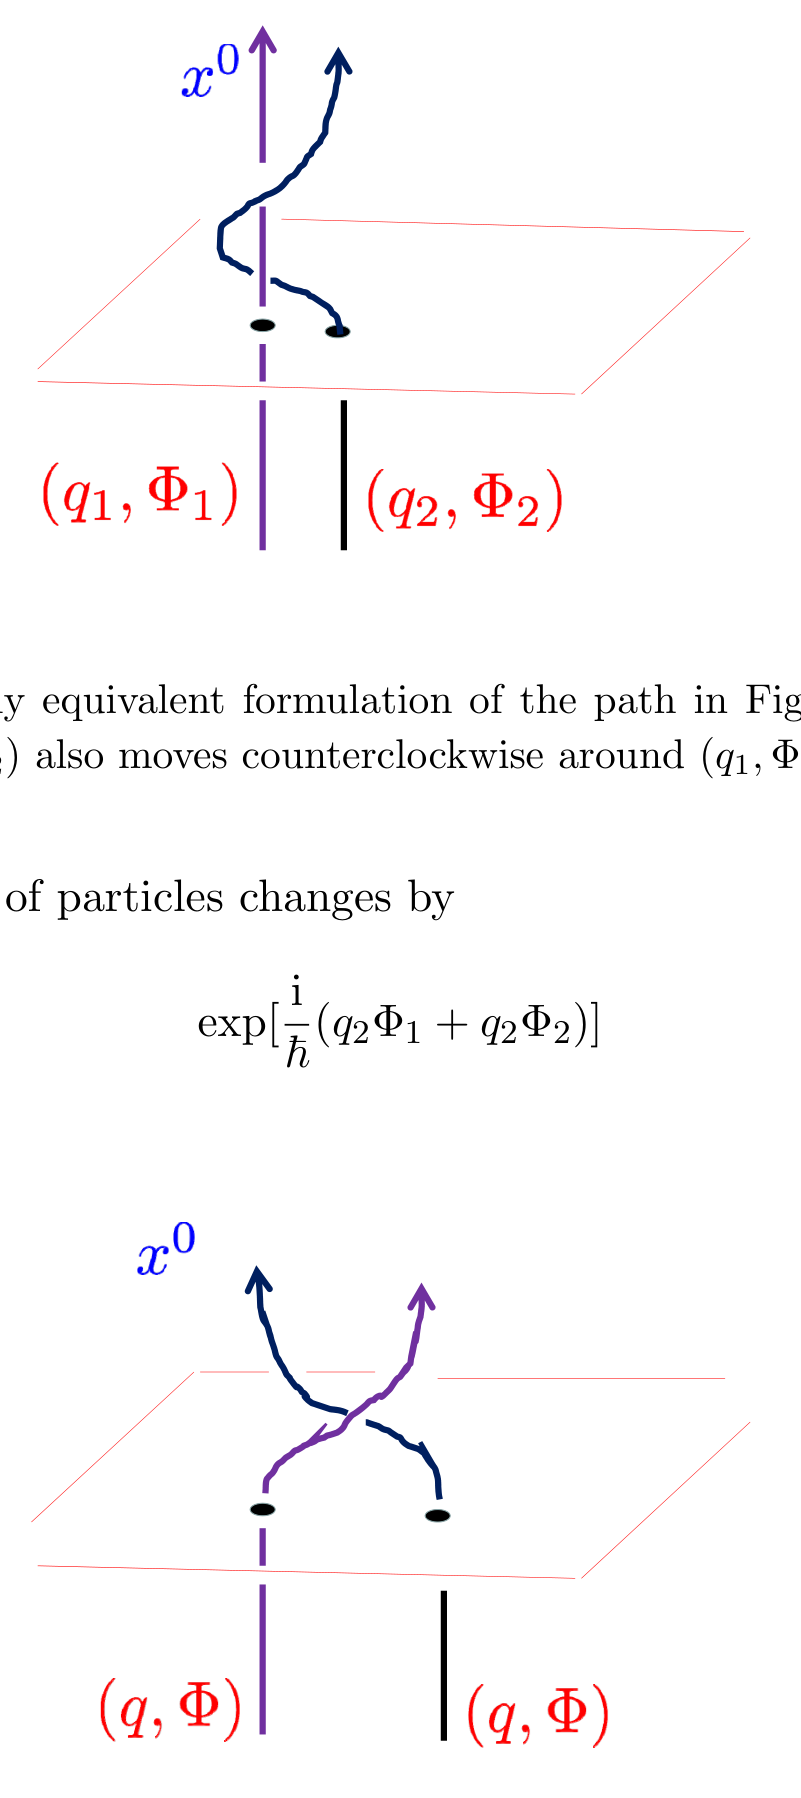
\includegraphics[width=0.6\textwidth]{figures/fig30.png}
  \caption{一对全同粒子 $(q,\Phi)$ 被交换。（原文 Fig.~30，第 163 页）}
  \label{fig:30}
\end{figure}

现在让我们考虑一对全同粒子，它们如图~\ref{fig:30} 所示被交换。净相位变化就是 $\exp[\mathrm{i}\frac{q\Phi}{\hbar}]$。但既然我们交换的是全同粒子，就可以把这个相位解释为统计相位。与 $3+1$ 维粒子的情形不同，在目前的情形下统计相位可以是\emph{任意}相位。这样的粒子称为任意子。\footnote{任意子的可能存在性由 Leinaas 与 Myrheim 于 1977 年指出。``anyon'' 一词则由 F. Wilczek 在 ``Quantum Mechanics of Fractional-Spin Particles''（Physical Review Letters \textbf{49} (14): 957-959）中提出。}

考察自旋与统计之间的关系是很有意思的。

现在我们把一般公式 (??) 用到 $d=2+1$ 维的角动量上。这里只有一个生成元 $J=J_{12}$。

在 $2+1$ 维中，螺线管贡献 $F_{ij}=\epsilon_{ij}\Phi\delta^2(x)$（这里 $i,j$ 取 $1$ 到 $2$，且 $\epsilon_{12}=+1$）。由 (??) 可知，位于 $\vec R$ 处的带电粒子贡献电场
\begin{equation}
  \vec E=2q\,\frac{\vec x-\vec R}{|\vec x-\vec R|^2}
  \tag{10.2}
  \label{eq:10.2}
\end{equation}
于是 $F_{0j}=-2q(x-R)^j/|\vec x-\vec R|^2$。因此动量密度为
\begin{equation}
  T_{0i}=F_{0k}F_{ik}=\frac{q\Phi}{2\pi}\epsilon_{ij}\frac{R_j}{R^2}\delta^{(2)}(\vec x)
  \tag{10.3}
  \label{eq:10.3}
\end{equation}
由于 $\delta$ 函数，积分很容易算出，我们得到
\begin{equation}
  J_{12}=\frac{q\Phi}{2\pi}\frac{\vec a\cdot\vec R}{\vec R\cdot\vec R}
  \tag{10.4}
  \label{eq:10.4}
\end{equation}
现在来检验自旋与统计的关系就很有趣了：
% [Tutor Note: (10.2)–(10.3) 中间那一步「$F_{0j}=-2q(x-R)^j/|\vec x-\vec R|^2$」里作者把矢量写成了标量 $(x-R)^j$（同页 (10.2) 用的是 $\vec x,\vec R$），转写时照原样保留。另外这一段用的显然是自然单位制（(10.3)、(10.4) 中没有 $c$），而 (10.1) 的相位里却出现了 $\hbar c$；核对量纲时请连同 $c$ 一起检查：作用是 $q\Phi/c$ 才与 $\hbar$ 同量纲]

\begin{figure}[htbp]
  \centering
  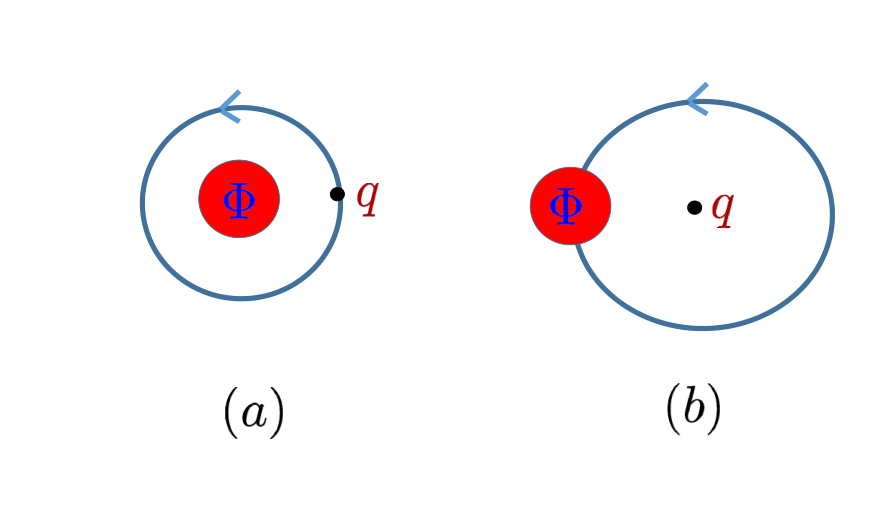
\includegraphics[width=0.8\textwidth]{figures/fig31.png}
  \caption{(a) 中电荷 $q$ 被缓慢地绕磁通子（fluxon）$\Phi$ 移动，波函数获得一个 Aharonov-Bohm 相位。(b) 中我们绕 $q$ 作一个 $2\pi$ 的旋转，电磁场的波函数也获得一个相位。这两个相位是相同的。（原文 Fig.~31，第 164 页）}
  \label{fig:31}
\end{figure}

\begin{enumerate}
  \item 若我们以逆时针方向缓慢地让粒子绕磁通转动，则波函数获得相位 $\exp[\mathrm{i}q\Phi/\hbar]$。
  \item 另一方面，若让磁通绕粒子转动，则波函数应当改变 $\exp[2\pi\mathrm{i}J/\hbar]$。在 \eqref{eq:10.4} 中取 $\vec a=\vec R$，我们得到同一个相位：
\end{enumerate}
\begin{equation}
  \exp[2\pi\mathrm{i}J/\hbar]=\exp[\mathrm{i}q\Phi/\hbar]
  \tag{10.5}
  \label{eq:10.5}
\end{equation}

\begin{remark}[自旋-统计定理]
证明自旋-统计定理时用到的重要性质，是存在到欧氏空间的解析延拓。
\end{remark}
% 原文此处是 "Remark Spin-statistics theorem: ..." 的格式；原文未给编号，译文用 remark 环境（编号由 LaTeX 自动给出）
{\small\itshape ［原文标记：Need to elaborate much more on that.（这一点需要再多讲很多。）］}
% [原文待办标记，原文 p.164；紧接在 remark 末句之后]

以下是一些关于任意子的更多材料来源：

\begin{enumerate}
  \item John Preskill 写了一些很好的讲义，其中讨论了与量子计算、量子信息理论的可能关联：\texttt{http://www.theory.caltech.edu/\textasciitilde presk}
  % 原文此行在 PDF 中被页面右边界截断（只印到 "presk"），译文照录截断后的字样
\end{enumerate}

% =====================================================================
%  c20 —— 原文印刷页 165（PDF 第 166 页）
%  含：第 10 节末尾「关于任意子的更多材料」文献列表的续接部分
%  （第 2--4 条与 OTHER REFS 速记清单），以及 Section 11
%  （11.1、11.2、11.3、11.4）的全部条目。
%  本片段无编号公式、无插图。
% =====================================================================

% 下列编号列表是从上一页（印刷 p.164）接续下来的：上一页在
% 「Here are some sources for more material about anyons:」之下已给出第 1 条
% （John Preskill 的讲义），本页从第 2 条起排，故用 start=2 复刻原编号。
\begin{enumerate}[start=2]
  \item 若要找一份相当新的综述，可参见 A. Stern，「Anyons and the quantum Hall effectA pedagogical review」，Annals of Physics 323: 204；arXiv:0711.4697v1。
  \item A. Lerda，\textit{Anyons: Quantum mechanics of particles with fractional statistics}，Lect. Notes Phys. M14 (1992) 1-138。
  \item 其它可参考的文献还包括：A. Khare，\textit{Fractional Statistics and Quantum Theory}；以及 G. Dunne，\textit{Self-Dual Chern-Simons Theories}。
\end{enumerate}

% [Tutor Note: 原文第 2 条里「effectA pedagogical review」处丢了一个句读——该综述（arXiv:0711.4697）的正式标题是「Anyons and the quantum Hall effect: A pedagogical review」，PDF 文本层与页面图像里冒号都被吞掉了（连字 ff 的排版所为）。此处照原样转写为 effectA，不加补；抄录文献时请以 arXiv 标题为准。另：原文该处用的是英式 ”…” 双引号，译文按本工程规范统一为「」。]

\textbf{其它文献（OTHER REFS）：}
\begin{itemize}[label={}]
  \item S. Buron，「A Short Guide to Anyons and Modular Functors」，
  \item 「From categories to anyons: a travelogue」
  \item Preskill
  \item Rowell 与 Wang：[52] BAMS
\end{itemize}

% [Tutor Note: 这块「OTHER REFS」是作者随手记下的补充读物清单，与上面那个编号列表不属于同一层，故单独排成无标号列表。四条都只给了残缺信息：「S. Buron」的拼写疑为笔误，「From categories to anyons: a travelogue」缺作者与出处，「Preskill」即上一页第 1 条已给出的 John Preskill 讲义，「Rowell and Wang: [52] BAMS」中的 [52] 是本文参考文献表的编号、BAMS 指 Bulletin of the American Mathematical Society。译文一律照原样保留，不作补全，以免替作者「猜出」文献。]

\section{进一步推广与应用的综述} % 原文: 11. A Survey Of Further Generalizations And Applications

\begin{keytakeaways}
  \item 本节是作者给出的一张「应用地图」：只列条目，不给推导，每条线索背后都是独立的一支研究文献。
  \item 超引力方向四条：RR 场与自对偶性、反常抵消、M 理论的 Chern-Simons 项，以及带边流形上 M 理论配合 $E_8$ 规范理论时的反常抵消。
  \item 非紧群方向：三维量子引力（Brown-Henneaux 与 Witten 的进路），以及把能级 $k$ 解析延拓、改用复群。
  \item 全息方向：$SL(2,\mathbb{R})$ 与单态表示（singleton）。
  \item 其它方向：格点费米子（David Kaplan）、算术 Chern-Simons（Minhyong Kim）、超群上的 Chern-Simons、与拓扑弦的关系（Marino 的综述 [39]）、CY 3-流形上的全纯 Chern-Simons 对应 B 模型开拓扑弦，以及弦场论。
\end{keytakeaways}

\subsection{在超引力中的应用} % 原文: 11.1 Applications To Supergravity

\begin{enumerate}
  \item RR 场与自对偶性
  \item 反常抵消。
  \item M 理论的 Chern-Simons 项。
  \item 带边流形上 M 理论（配合 $E_8$ 规范理论）的反常抵消。
\end{enumerate}

% [Tutor Note: 第一条的「RR 场」是 Ramond--Ramond 场（原文只写缩写），即 II 型超引力中的那些反对称张量场；「自对偶性」指其场强满足一阶自对偶约束 $*F=\pm F$（例如 IIB 五形式场强），这类约束无法由普通的二阶（度规型）作用量变分得到，必须改用 Chern-Simons 型拓扑项来写，这正是 CS 理论在此处登场的原因。本节四条都只是标题，作者未展开任何一条，故此处不补推导。]

\subsection{非紧群} % 原文: 11.2 Noncompact Groups

三维量子引力：
\begin{itemize}[label={}]
  \item Brown-Henneaux
  \item Witten 处理三维量子引力的诸种进路。
  \item 在 $k$ 上的解析延拓：复群。
\end{itemize}

% [Tutor Note: 「在 $k$ 上的解析延拓」指把 CS 能级 $k$ 当作复参数：对紧群，$k$ 必须是整数（作用量的 $2\pi$ 整性、以及标架反常给出的平移 $k\to k+h^\vee$ 都需要它），而一旦允许复 $k$、乃至把规范群复化，这套整性条件与度规的正定假设都要重新检查——这是非紧群条目下最易被忽略的一句。作者在此只点了线索，细节需查 Witten 关于三维引力的原文。]

\subsection{在全息中的应用} % 原文: 11.3 Applications to Holography

$\mathrm{SL}(2,\mathbb{R})$

单态表示（singletons）

% [Tutor Note: 原文这两行分别印作直立的「SL(2,R)」与「Singletons」，此处把 R 排成 $\mathbb{R}$ 只是记号规范化。术语上 singleton（Dirac 的「单态」表示，即 $SO(2,d)$ 的超轻表示）若直译成「单态」易与 $J=0$ 的那种单态混淆，故保留英文并附中文；下文若再出现同一词，不再重复括注。]

\subsection{许多其它应用与推广} % 原文: 11.4 Many Other Applications And Extensions

\begin{enumerate}
  \item 格点费米子（David Kaplan）
  \item 算术 Chern-Simons（Minhyong Kim）
  \item 超群上的 Chern-Simons
  \item Chern-Simons 与拓扑弦。参见 Marino 的综述 [39]。
  \item CY 3-流形上的全纯 Chern-Simons：B 模型开拓扑弦
  \item 弦场论
\end{enumerate}

% [Tutor Note: 第五条极易读错：「CY 3-folds」是复三维 Calabi-Yau 流形，实维数为 6，因此其上的全纯 Chern-Simons 是一个六维作用量，与前面三维 CS 不是同一个理论，不能把三维的 $k$ 量子化、Wilson 线等结论直接搬来；「B 模型」指拓扑 B 模型，其开弦（也就是拓扑弦）由全纯 CS 描述，这一点正是它被列入「推广」而非「应用」的原因。]


%% ---------- 附录：编号切换为 A, B, C, ... ----------
\appendix
% =====================================================================
%  c21 —— 原文印刷页 166–171（PDF 第 167–172 页）
%  附录 A 的开头：A. Symplectic Geometry（A.1 Kähler quotients 的
%  A.1.1 The moment map、A.1.2 Symplectic Quotient、A.1.3 Kähler quotient）
%  与 B. Lightning Review Of Kähler Quantization 的 B.1 The Bargmann
%  Representation。本片段无插图。
%  main.tex 已在本片段之前发出 \appendix，故此处只用 \section/\subsection/
%  \subsubsection，编号 A、A.1、A.1.1 由 LaTeX 自动给出。
% =====================================================================

\section{辛几何} % 原文: A. Symplectic Geometry

\begin{keytakeaways}
  \item 物理图像：相空间就是一个辛流形 $(M,\omega)$，即带有非退化二形式的流形；$\omega$ 的逆给出 Poisson 括号 (A.2)，于是经典力学的运动学完全编码在 $\omega$ 里，度规并不出现。
  \item 数学工具：Darboux 定理说明辛形式没有非平凡的局部不变量，辛结构的信息全是整体的；连续对称性则由矩映射 $\mu:M\to\mathfrak{g}^*$ 承载，(A.10) 把「每条生成元对应一个守恒荷」写成配对，(A.11) 要求它关于余伴随作用等变。
  \item 核心结论：辛商（Hamilton 约化）$M/\!/_\zeta G=\mu^{-1}(\zeta)/G$ (A.30) 给出约化后的相空间；而 Poisson 括号给出的 Lie 代数 2-上循环 $c^{AB}$ (A.26) 若代表非平凡上同调类，则同时施加第一类约束会遇到反常。
  \item 关键例子：$\mathbb{C}^N$ 上按权 $Q^a$ 的 $U(1)$ 作用，商空间的性质由 $Q^a$ 的可公度性、互素性与符号决定——权两两互素时商空间光滑，出现公共因子时留下 $\mathbb{Z}_r$ 轨形奇点，而权异号时约束面非紧；当 $Q_a=\pm1$ 时辛商是 $\mathcal{O}(1)$ 丛的全空间。
  \item 与场论的联系：超对称场论势能中的 $D$ 项恰好是靶空间上 $G$-作用的矩映射，矩映射的能级 $\zeta^A$ 就是 Fayet–Iliopoulos 项。
\end{keytakeaways}

回忆：相空间是一个辛流形（symplectic manifold），即带有非退化二形式
\begin{equation}
  \omega=\frac{1}{2}\omega_{\mu\nu}dx^{\mu}\wedge dx^{\nu}
  \tag{A.1}
  \label{eq:A.1}
\end{equation}
的流形；由此可以定义相空间上两个函数的 Poisson 括号：
\begin{equation}
  \{f_1,f_2\}=\omega^{\mu\nu}\frac{\partial f_1}{\partial x^{\mu}}\frac{\partial f_2}{\partial x^{\nu}}
  \tag{A.2}
  \label{eq:A.2}
\end{equation}

辛几何的第一个主要定理是：辛形式没有非平凡的局部不变量。这就是 Darboux 定理：它说在 $\mathcal{P}$ 上总存在局部坐标 $(p_i,q^i)$，使得
\begin{equation}
  \omega=\sum_i dp_i\wedge dq^i
  \tag{A.3}
  \label{eq:A.3}
\end{equation}
{\small\itshape ［原文标记：$\clubsuit$这并不难证明。要不要给出证明？$\clubsuit$］}
% [原文待办标记，原文 p.166 页边竖排；作者在此自问是否补上 Darboux 定理的证明，最终未补]

相空间是讨论经典力学的恰当舞台，也是通向量子化的良好出发点。

\subsection{Kähler 商：快速回顾} % 原文: A.1 Kahler quotients: A lightning review

\subsubsection{矩映射} % 原文: A.1.1 The moment map

设 $(M,\omega)$ 是一个相空间，即一个辛流形。

回忆：给定 $M$ 上的函数 $h$，可以由 $\iota(V)\omega=dh$ 作出与之对应的 Hamilton 向量场；用局部坐标写出就是
\begin{equation}
  V^i=\omega^{ij}\partial_j h
  \tag{A.4}
  \label{eq:A.4}
\end{equation}
% [Tutor Note: 符号约定易错。(A.2) 把 Poisson 括号定义为 $\{f,g\}=\omega^{ij}\partial_if\,\partial_jg$，而 (A.4) 取 $V^i=\omega^{ij}\partial_jh$，即 $\iota(V)\omega=dh$。直接代入会得到 $V_\mu(f)=-\{\mu,f\}=\{f,\mu\}$，与 (A.8) 第一行到第二行所默认的 $\{\mu,f\}=\xi^i\partial_if$ 差一个负号。核对时请把 (A.2)、(A.4)、(A.8) 三式并排验证（用 $\omega^{12}=1$、$\mu=x^1$、$f=x^2$ 试算即可看出）；作者本人在 p.171 的 (B.1) 旁也标了「SIGN???」，可见他对符号是随手处理的]

向量场 $V$ 生成一个保持辛形式的微分同胚群。

反过来，设 $(M,\omega)$ 是辛流形，且 Lie 群 $G$ 辛作用（acts symplectically）：
\begin{equation}
  g^{*}(\omega)=\omega\qquad\forall g\in G
  \tag{A.5}
  \label{eq:A.5}
\end{equation}

把这一点用到由 $T\in\mathfrak{g}$ 生成的单参数子群上，便得到向量场 $\xi=\xi(T)$，使得
\begin{align}
  0 &= \mathcal{L}_{\xi}\omega \notag\\
    &= \big(d\iota(\xi)+\iota(\xi)d\big)\omega \label{eq:A.6}\tag{A.6}\\
    &= d\big(\iota(\xi)\omega\big) \notag
\end{align}

因此，若 $H^{1}_{DR}(M)=0$，我们就可以断定
\begin{equation}
  \iota(\xi)\omega=d\mu
  \tag{A.7}
  \label{eq:A.7}
\end{equation}
其中 $\mu:M\to\mathbb{R}$ 是某个整体良定义的函数。注意 $\mu$ 只定义到相差一个常数。它依赖于 $T$，所以我们把它在一点处的值记作 $\mu(p;T)$，$p\in M$、$T\in\mathfrak{g}$。

在 Hamilton 动力学中，$\mu$ 就是与向量场 $\xi$ 所生成对称性相应的荷（charge）。它生成与该对称性相联系的变换：
\begin{align}
  \{\mu,f\} &= \omega^{ij}\partial_i\mu\,\partial_jf \notag\\
           &= \xi^i\partial_if \label{eq:A.8}\tag{A.8}\\
           &= \mathcal{L}_{\xi}(f) \notag
\end{align}
其中最后一行用到了关于 $\xi$ 的 Lie 导数。

对每个元素 $T\in\mathfrak{g}$，我们都有一个守恒荷 $\mu(\cdot;T)$。由于 $T\mapsto\xi(T)$ 关于 $T$ 线性，$T\mapsto\mu(\cdot;T)$ 也关于 $T$ 线性。以「关于 $T$ 线性」的方式对每个 $T\in\mathfrak{g}$ 给出一个函数 $M\to\mathbb{R}$，等价于给出单个函数
\begin{equation}
  \mu:M\to\mathfrak{g}^{*}
  \tag{A.9}
  \label{eq:A.9}
\end{equation}

这个函数称为矩映射（moment map）。按定义它对一切 $T\in\mathfrak{g}$ 满足
\begin{equation}
  \langle T,\mu(p)\rangle:=\mu(p;T)
  \tag{A.10}
  \label{eq:A.10}
\end{equation}
此外还有
\begin{equation}
  \mu(g\cdot p)=\operatorname{Ad}^{*}(g)\big(\mu(p)\big)
  \tag{A.11}
  \label{eq:A.11}
\end{equation}
其中右端是余伴随作用（coadjoint action）。
% [Tutor Note: 术语取舍。"moment map" 的中文译法有「矩映射」「动量映射」「矩量映射」三种；此处统一取「矩映射」，因为它保留 "moment"（而非 momentum）的字面，也与本文后面 $D$ 项、Fayet–Iliopoulos 项的语境相容。作者紧接着自己解释 "the word 'moment' is short for 'momentum'"，故正文首次出现处括注英文原词，读者可自行对照]

取 $\mathfrak{g}$ 的一组基 $T^A$，我们可以写
\begin{equation}
  \mu=\sum_A\mu^A T^{*}_A
  \tag{A.12}
  \label{eq:A.12}
\end{equation}
其中 $\mu^A=\mu(T^A)$ 是 $M$ 上的普通函数。

“moment” 一词是 “momentum” 的缩写。它可以是线动量，也可以是角动量，如下面的例子所示：

\textbf{例 1}：设 $M=T^{*}\mathbb{R}^n$，取 Darboux 坐标 $(\vec{q},\vec{p})=(\vec{q}^{\,i},\vec{p}_i)$，于是
\begin{equation}
  \omega=\sum_i dp_i\wedge dq^i
  \tag{A.13}
  \label{eq:A.13}
\end{equation}

设 $G=\mathbb{R}^n$ 通过平移作用：
\begin{equation}
  \vec{a}\cdot(\vec{q},\vec{p})=(\vec{q}+\vec{a},\vec{p})
  \tag{A.14}
  \label{eq:A.14}
\end{equation}

我们还有：作为向量空间 $\mathfrak{g}\cong\mathbb{R}^n$，其 Lie 括号恒为零，而无穷小作用由 $g(t)=e^{t\vec{v}}$ 给出：
\begin{equation}
  g(t):(\vec{q},\vec{p})\to(\vec{q}+t\vec{v},\vec{p})
  \tag{A.15}
  \label{eq:A.15}
\end{equation}

于是
\begin{equation}
  \xi(\vec{v})=v^i\frac{\partial}{\partial q^i}
  \tag{A.16}
  \label{eq:A.16}
\end{equation}

并且
\begin{equation}
  \iota\big(\xi(\vec{v})\big)\omega=-v^idp_i=d\mu(\vec{v})
  \tag{A.17}
  \label{eq:A.17}
\end{equation}
其中
\begin{equation}
  \mu(q^i,p_i;\vec{v})=-v^ip_i
  \tag{A.18}
  \label{eq:A.18}
\end{equation}

\textbf{例 2} 转向我们的主要例子：设 $G$ 线性作用在向量空间 $V=\{(x^1,\dots,x^N)\}$ 上，辛形式为 $\omega_{ij}dx^idx^j$，其中 $\omega_{ij}$ 是常值反对称矩阵。设 $\rho(T^A)^i{}_j$ 是表示该 Lie 代数的 $N\times N$ 矩阵。则
\begin{equation}
  \xi^A:=\xi(T^A)=x^j\rho(T^A)^i{}_j\frac{\partial}{\partial x^i}
  \tag{A.19}
  \label{eq:A.19}
\end{equation}

于是矩映射为
\begin{equation}
  \mu^A(x)=\frac{1}{2}x^j\rho(T^A)^i{}_j\omega_{ik}x^k
  \tag{A.20}
  \label{eq:A.20}
\end{equation}
% [Tutor Note: (A.20) 的因子 $1/2$ 来自「对 $x^j\omega_{ik}x^k$ 求微分后除以 2」：把 (A.20) 代入 $d\mu^A=\iota(\xi^A)\omega$，用到 $\omega_{ik}$ 反对称与紧接 (A.20) 之后那句「$\rho(T^A)^i{}_j\omega_{ik}$ 关于 $jk$ 对称」，两份贡献相加恰好抵消 $1/2$。若漏掉那条对称性条件，就会算出多一个因子 2]

（该群辛作用，当且仅当矩阵 $\rho(T^A)^i{}_j\omega_{ik}$ 关于 $jk$ 对称。）

特殊化到 $M=T^{*}\mathbb{R}^n$ 并取标准 Darboux 坐标的情形，我们可以考虑嵌入 $GL(n,\mathbb{R})\hookrightarrow Sp(2n,\mathbb{R})$，其中
\begin{equation}
  \begin{pmatrix}
    A & \\
      & A^{tr,-1}
  \end{pmatrix}
  \tag{A.21}
  \label{eq:A.21}
\end{equation}
% [Tutor Note: (A.21) 的记法 $A^{tr,-1}$ 应读作 $(A^{\mathrm{tr}})^{-1}$（等价于 $(A^{-1})^{\mathrm{tr}}$），不是「$A^{\mathrm{tr}}$ 减 1」；整个块矩阵是 $\mathrm{diag}\big(A,(A^{\mathrm{tr}})^{-1}\big)$，它保持 (A.13) 的 $\sum_i dp_i\wedge dq^i$。原文把转置与求逆压进一个上标，转写时若不还原，读者无法判断第二块到底是 $A^{\mathrm{tr}}$ 还是 $A^{-1}$]

对群元素 $g(t)=1+te_{ij}\in GL(n,\mathbb{R})$，我们有
\begin{equation}
  g(t):(\vec{q},\vec{p})\to(\vec{q}+tq_j\vec{e}_i,\ \vec{p}-tp_i\vec{e}_j)
  \tag{A.22}
  \label{eq:A.22}
\end{equation}
于是
\begin{equation}
  \xi(e_{ij})=q^j\frac{\partial}{\partial q^i}-p_i\frac{\partial}{\partial p_j}
  \tag{A.23}
  \label{eq:A.23}
\end{equation}
并且
\begin{equation}
  \mu(q^i,p_i;e_{ij})=-q^ip_j
  \tag{A.24}
  \label{eq:A.24}
\end{equation}

若进一步特殊化到 $SO(n)\subset GL(n,\mathbb{R})$、取基 $T_{ij}=e_{ij}-e_{ji}$，我们得到 $\mu(T_{ij})=q^jp_i-q^ip_j$；最后特殊化到 $T^{*}\mathbb{R}^3$、取 $T_i=\frac{1}{2}\epsilon_{ijk}T_{jk}$，我们发现 $\mu(T_i)=L_i$ 正是角动量的标准公式：
\begin{equation}
  \mu(q^i,p_i;T_i)=\epsilon_{ijk}q^jp_k
  \tag{A.25}
  \label{eq:A.25}
\end{equation}

\subsubsection{辛商} % 原文: A.1.2 Symplectic Quotient

若 $H^{1}_{DR}(M)=0$，可以证明
\begin{equation}
  \{\mu^A,\mu^B\}=f_C^{AB}\mu^C+c^{AB}
  \tag{A.26}
  \label{eq:A.26}
\end{equation}
其中 $c^{AB}$ 为某些常数。Poisson 括号上的 Jacobi 关系表明，这些 $c^{AB}$ 事实上定义了一个 Lie 代数 2-上循环（2-cocycle）。把 $\mu^A$ 平移常数，会把该上循环重新定义到相差一个上边缘（coboundary）。如果该 2-上循环为零，那么我们就能像在约束 Hamilton 动力学中那样同时施加约束 $\mu^A=0$。如果该 2-上循环代表一个非平凡的上同调类，那么「试图施加这些约束」就会遇到反常（anomaly）。

我们假定可以通过上边缘的平移把任何上循环 $c^{AB}$ 归零。若 $\zeta\in Z(\mathfrak{g})^{*}$ 落在中心（……的对偶）之中，则约束 $\phi=\mu-\zeta$ 是第一类约束（first class constraints）。也就是说，约束集合
\begin{equation}
  \phi^A=\mu(T^A)-\langle T^A,\zeta\rangle=0
  \tag{A.27}
  \label{eq:A.27}
\end{equation}
构成一组第一类约束。
% [Tutor Note: 原文此句为 "If $\zeta\in Z(\mathfrak g)^*$ is in the (dual of ) the center"，括号里明显漏了一个词或符号，原 PDF 上就是空白；译文照原样保留空缺。按上下文应读作「$\zeta$ 属于 $\mathfrak g$ 的中心 $Z(\mathfrak g)$ 的对偶」，即 $\zeta$ 只在中心上与生成元配对。这正是 $\phi^A$ 两两第一类（$\{\phi^A,\phi^B\}=f_C^{AB}\phi^C$）的条件，请对照 (A.26) 与 (A.28) 核实]

现在，取 $c^{AB}=0$ 的式 \eqref{eq:A.26} 给出
\begin{equation}
  \mathcal{L}_{V^A}(\mu^B)=f_C^{AB}\mu^C
  \tag{A.28}
  \label{eq:A.28}
\end{equation}
% [Tutor Note: (A.28) 左端的 $V^A$ 是 (A.4) 意义下 $\mu^A$ 的 Hamilton 向量场；这一步只是把 (A.26) 改写成 Lie 导数形式，$\mathcal{L}_{V^A}\mu^B$ 与 $\{\mu^A,\mu^B\}$ 至多差一个符号（取决于 $\iota(V)\omega=dh$ 的约定，见 (A.4) 处的批注）。若 $c^{AB}\neq0$，右端还要多出 $c^{AB}$，那正是「第二类约束／反常」的来源。另注意原文把结构常数排成 $f_C^{AB}$（上上／下），并非通常的 $f^{AB}{}_C$；引用时按 (A.26) 里与 $\mu^C$ 的缩并来配对，不要按上下标位置另设约定]

因此，若 $G$ 连通，我们就能断定：由 \eqref{eq:A.27} 所定义的相空间中的约束空间
\begin{equation}
  \mathcal{S}:=\{p\,|\,\phi^A(p)=0\}\subset M
  \tag{A.29}
  \label{eq:A.29}
\end{equation}
是 $G$-不变的。于是我们可以对 $G$-作用取商。

\textbf{定义} $M$ 关于 $G$ 的辛商（symplectic quotient）——或称 Hamilton 约化（Hamiltonian reduction）——是如下流形：
\begin{equation}
  M/\!/_{\zeta}G=\mu^{-1}(\zeta)/G
  \tag{A.30}
  \label{eq:A.30}
\end{equation}

\subsubsection{Kähler 商} % 原文: A.1.3 Kähler quotient

回忆：Kähler 流形是带有相容复结构 $I$ 的 Riemann 流形，即 $g(IX,IY)=g(X,Y)$（$X,Y\in TM$），且该复结构关于 Levi-Civita 联络平行，$\nabla I=0$。等价地，由 $\omega(X,Y)=g(X,IY)$ 定义的二形式是闭 2-形式。

用坐标来说：存在局部复坐标 $z^i$，使得 $ds^2=g_{i\bar{j}}dz^i\otimes d\bar{z}^{\bar{j}}+cc$，并且
\begin{equation}
  \omega=\frac{\mathrm{i}}{2}g_{i\bar{j}}dz^i\wedge d\bar{z}^{\bar{j}}
  \tag{A.31}
  \label{eq:A.31}
\end{equation}
是闭 2-形式。

当然，Kähler 流形就是带有辛形式 $\omega$ 的辛流形。

\textbf{定理}：设 $M$ 是 Kähler 流形，且 $G$ 无不动点地辛作用。那么辛商是光滑的 Kähler 流形，其 Kähler 结构继承自 $M$。

证明见所引文献。
% [Tutor Note: 作者以 "For a proof see the references" 跳过证明。这条定理是 Kempf–Ness 定理的 Kähler 版（即 Marsden–Weinstein 约化的复几何表述）：完整陈述还需要 $G$ 紧致、作用自由且 proper，原文的 "without fixed points" 只交代了自由性的一半；结论「辛商光滑并继承 Kähler 结构」依赖 $\mu^{-1}(\zeta)/G$ 与复商 $M^{\mathrm{stable}}/G$ 的同构，建议查 Kempf–Ness (1978) 或 Mumford《Geometric Invariant Theory》]

其一个重要特例如下。取 $V=\mathbb{C}^N$ 为复向量空间，辛形式为
\begin{equation}
  \omega=\frac{\mathrm{i}}{2}\sum_{a=1}^{N}dz^a\wedge d\bar{z}_a=\sum_a dx^a\wedge dy^a
  \tag{A.32}
  \label{eq:A.32}
\end{equation}
其中 $z^a=x^a+\sqrt{-1}\,y^a$。显然，这一形式在 $U(N)$ 作用于 $z^a$ 时保持不变。Lie 代数的一个元素是反 Hermite 矩阵
\begin{equation}
  (T^a{}_b)^{*}=-T^b{}_a
  \tag{A.33}
  \label{eq:A.33}
\end{equation}
相应的向量场是
\begin{equation}
  \xi(T)=z^bT^a{}_b\frac{\partial}{\partial z^a}-\bar{z}_b(T)^b{}_a\frac{\partial}{\partial\bar{z}_a}
  \tag{A.34}
  \label{eq:A.34}
\end{equation}
而相应的动量是
\begin{equation}
  \mu(T)=\mathrm{i}z^bT^a{}_b\bar{z}_a
  \tag{A.35}
  \label{eq:A.35}
\end{equation}
（相差一个常数）。

\textbf{例 1} $V=\mathbb{C}^N$，带有辛形式 \eqref{eq:A.32}，$G=U(1)$ 通过
\begin{equation}
  e^{\mathrm{i}\theta}:z^a\to e^{\mathrm{i}Q^a\theta}z^a,\qquad a=1,\dots,N
  \tag{A.36}
  \label{eq:A.36}
\end{equation}
作用。矩映射为
\begin{equation}
  \mu=\sum Q^a|z^a|^2
  \tag{A.37}
  \label{eq:A.37}
\end{equation}

辛商的性质强烈依赖于 $Q^a$ 以及矩映射的能级 $\zeta$：

\begin{enumerate}[label={\alph*.)},leftmargin=2.4em,itemsep=2pt]
  \item 除非 $Q^a$ 彼此可公度，$U(1)$ 作用是遍历的（ergodic）。让我们设 $Q^a$ 可公度。于是我们可以写 $Q^a=p^a/L$，其中 $L$ 为某个整数，且 $\mathrm{g.c.d}(p^1,\dots,p^N)=1$。商的性质依赖于整数 $p^i$。若它们两两互素，则商空间是光滑的。然而，假设存在子集 $S\subset\{1,\dots,N\}$，在其上 $p^a=rq^a$，其中 $r$ 为某个公因子。若对 $b\notin S$ 有 $z^b=0$，并取 $\theta=2\pi/r$，则该群有不动点。于是我们得到 $\mathbb{Z}_r$ 轨形奇点。
  \item 若一切 $Q^a$ 都为正且为有理数，并且 $\zeta>0$，则约束空间 $\mu=\zeta$ 是紧的且非空。它是一个形变球面。
  \item 若 $Q^a$ 符号不同，则约束空间非紧，并且可能出现非常不同的现象。
\end{enumerate}

这个例子也说明了 Kähler 商的拓扑如何随能级 $\zeta$ 的改变而改变。设有 $n_+$ 个 $Q_a=+1$ 与 $n_-$ 个 $Q_a=-1$。那么当 $\zeta>0$ 时辛商是丛 $\mathcal{O}(1)^{\oplus n_-}\to\mathbb{CP}^{n_+-1}$ 的全空间，而当 $\zeta<0$ 时它是 $\mathcal{O}(1)^{\oplus n_+}\to\mathbb{CP}^{n_--1}$。

\textbf{例 2} 超对称场论中的 $D$ 项。设我们有一个四维、带有四个超对称的超对称场论，其中有一组手征超场（chiral superfields）$\Phi^a$，它们按规范群的某个酉表示变换，该群的生成元为 $T^A$。设手征超场取值于一个线性空间，并具有标准的 Kähler 势 $\sum|\Phi^a|^2$。则势能中的 $D$ 项 $D^A$ 恰好是靶空间上 $G$-作用的矩映射。矩映射的能级 $\zeta^A$ 与 $G$ 中的 $U(1)$ 因子相联系，称为 Fayet–Iliopoulos 项。

{\small\itshape ［原文标记：*********************************］}
% [原文待办标记，原文 p.170 页末；原稿在此用一整行星号表示「此处还缺内容」，星号之后本片段结束]

\section{Kähler 量子化速览} % 原文: B. Lightning Review Of Kähler Quantization

\begin{keytakeaways}
  \item 出发点：标准相空间 $\mathcal{P}=\mathbb{R}^2$（坐标 $(q,p)$、辛形式 $\omega=dp\wedge dq/2\pi\hbar$，即 (B.1)），由此导致标准的 $[\hat{p},\hat{q}]=-\mathrm{i}\hbar$。
  \item 与通常量子化的差别：通常取 $\mathcal{H}=L^2(\mathbb{R})$，且为一般函数 $f(p,q)$ 定义 $Q(f)$ 必须额外选一套算符排序规定，以满足判据 (2.75)–(2.78)；Bargmann 表示改用 $\mathcal{H}=\mathrm{Hol}(\mathbb{C})$，即复平面上的整函数空间。
  \item 核心构造：内积带 Gaussian 权 $e^{-\kappa|z|^2}$ (B.2)，$\kappa>0$ 扮演 $1/\hbar$；一般（不必全纯的）可积函数 $f(z,\bar{z})$ 的量子化由积分核 (B.4) 给出，其算符形式为 $Q^{(\kappa)}(f)=\Pi\circ M_f\circ\iota$。
  \item 代数实现：取 $a=\sqrt{\kappa}\,Q^{(\kappa)}(\bar{z})$、$a^\dagger=\sqrt{\kappa}\,Q^{(\kappa)}(z)$ (B.5)，则 $[a,a^\dagger]=1$ (B.6)——即 $a$ 与 $a^\dagger$ 分别由「乘以 $\bar{z}$ 后投影」与「乘以 $z$ 后投影」实现。
\end{keytakeaways}

\subsection{Bargmann 表示} % 原文: B.1 The Bargmann Representation

Bargmann 表示是量子化标准相空间 $\mathcal{P}=\mathbb{R}^2$ 的另一种方式；该相空间的坐标为 $(q,p)$，辛形式为
\begin{equation}
  \omega=\frac{dp\wedge dq}{2\pi\hbar}
  \tag{B.1}
  \label{eq:B.1}
\end{equation}
由此得到标准的 $[\hat{p},\hat{q}]=-\mathrm{i}\hbar$。{\small\itshape ［原文标记：$\clubsuit$符号？？？$\clubsuit$］}
% [原文待办标记，原文 p.171 页边；作者自己怀疑 (B.1) 与对易子的符号约定]

在通常的量子化中，我们把 $\mathcal{P}=T^{*}\mathbb{R}$ 看作带有实轴上坐标 $q$ 的相空间，于是 $\mathcal{H}=L^2(\mathbb{R})$，波函数是可归一化的函数 $\psi(q)$，而 $\hat{p}=-\frac{\mathrm{i}}{\hbar}\frac{d}{dq}$，等等。为了对一般函数 $f(p,q)$ 定义 $Q^{(k)}(f)$，必须选取一套算符排序（operator ordering）规定；这可以用若干种方式做到，以满足上文所列的判据 \eqref{eq:2.75}–\eqref{eq:2.78}。

在 Bargmann 表示中，Hilbert 空间则取为 $\mathcal{H}=\mathrm{Hol}(\mathbb{C})$，即复平面上全体整函数构成的空间，其在如下定义的内积下可归一化：
\begin{equation}
  \langle\psi_1,\psi_2\rangle=\int_{\mathbb{C}}e^{-\kappa|z|^2}\psi_1(z)^{*}\psi_2(z)\,\omega
  \tag{B.2}
  \label{eq:B.2}
\end{equation}

这里 $\kappa>0$ 将扮演 $1/\hbar$ 的角色，而
\begin{equation}
  \omega=\frac{\mathrm{i}\,dz\wedge d\bar{z}}{2\pi}=\frac{dx\,dy}{\pi}=\frac{d\phi}{2\pi}d(r^2)
  \tag{B.3}
  \label{eq:B.3}
\end{equation}

可积函数 $f(z,\bar{z})$（\underline{不}必全纯或反全纯）的量子化 $Q^{(k)}(f)$ 由下式定义
\begin{equation}
  \langle\psi_{j_1}|Q^{(\kappa)}(f)|\psi_{j_2}\rangle=\int_{\mathbb{C}}e^{-\kappa|z|^2}\psi_{j_1}^{*}(\bar{z})f(z,\bar{z})\psi_{j_2}(z)\,\frac{dx\,dy}{\pi}
  \tag{B.4}
  \label{eq:B.4}
\end{equation}
% [Tutor Note: (B.4) 印刷为 $\psi^{*}_{j_1}(\bar{z})$，但 $\psi_{j_1}\in\mathrm{Hol}(\mathbb{C})$ 是全纯函数，按 (B.2) 的内积此处应是 $\psi^{*}_{j_1}(z)$；页面图像上确实印着 $\bar z$，故照录。同一页还有 $Q^{(k)}$ 与 $Q^{(\kappa)}$ 混用（(B.4) 前的正文写 $Q^{(k)}$，而 (B.4)、(B.5) 写 $Q^{(\kappa)}$），二者指同一个参数，即 (B.2) 中扮演 $1/\hbar$ 的 $\kappa$]

特别地，若我们定义
\begin{equation}
  a=\sqrt{\kappa}\,Q^{(\kappa)}(\bar{z}),\qquad a^{\dagger}=\sqrt{\kappa}\,Q^{(\kappa)}(z)
  \tag{B.5}
  \label{eq:B.5}
\end{equation}
那么我们就能验证通常的关系
\begin{equation}
  [a,a^{\dagger}]=1
  \tag{B.6}
  \label{eq:B.6}
\end{equation}

{\small\itshape ［原文标记：*********************************\newline
关于相干态的一些评注。它们为何对半经典计算有用。\newline
BEREZIN 变换。\newline
*********************************］}
% [原文待办标记，原文 p.171 页末；原稿在两行星号之间列出了三点待补内容（相干态、半经典计算的用处、Berezin 变换），此处照原样保留]

% =====================================================================
%  c22 —— 原文印刷页 172–181（PDF 第 173–182 页）
%  含：B.2 推广：Berezin-Toeplitz 量子化（及 B.2.1 球面的量子化与 SU(2) 的表示）、
%      B.3 Borel-Weil-Bott 定理、附录 C 关于 SL(2,Z) 的一些细节（C.1、C.2）；
%      插图 Fig. 32（钥匙孔区域）。
% =====================================================================

\subsection{推广：Berezin-Toeplitz 量子化} % 原文: B.2 Generalization: Berezin-Toeplitz Quantization

% 本片段中 B.2、B.3 均为 \subsection 级（节级标题 B. 在前一片段 c21 中），
% 按规范「本节重点」只加在 \section 开头，故这两个小节的要点记在此处备忘：
% (i) 适用条件：相空间除辛结构外还带有相容的复结构 $J$（使 $\omega$ 成为正的 $(1,1)$ 形式），
%     且 $\omega$ 可取为全纯线丛 $L$ 上 Hermitian 联络的曲率，于是几何量子化化为
%     「全纯截面空间 $\mathcal{H}_\kappa=\ker\bar\partial$ 加 $L^2$ 内积」，$\hbar=1/\kappa$；
% (ii) 量子化映射 $Q^{(\kappa)}(f)=\Pi\circ M_f\circ\iota$，矩阵元见 (B.20)；
% (iii) 辛体积有限 $\Rightarrow$ 有限维 $\mathcal{H}$；把 $\omega/2\pi$ 认作 $c_1(\mathcal{L})$，
%     指标公式 (B.24)（Hirzebruch--Riemann--Roch）在 $\mathcal{L}$ 充分正、高阶上同调消没时给出精确维数，
%     其 $k\to\infty$ 展开 (B.25) 首项即「每 $2\pi\hbar$ 体积一个态」的 Bohr--Sommerfeld 规则，
%     下一阶符号由 $c_1(T^{1,0}\mathcal{P})$ 决定（正曲率增加、负曲率减少量子态数）；
% (iv) 范例 $S^2=\mathbb{CP}^1=SU(2)/U(1)$：取 $K=\log(1+|z|^2)$ 时 $\mathcal{H}_\kappa$ 为 $\kappa+1$ 维，
%     即 $\mathbf{su}(2)$ 的自旋 $j=\kappa/2$ 不可约表示，而辛体积给出的是 $2j$。

当相空间额外带有 Kähler 流形的结构时，有一种非常漂亮的量子化程序可用，它在 Chern-Simons 理论中极其有用。关于 Berezin-Toeplitz 量子化的描述，可参见例如 [53] 及其所引文献。

回忆一下：辛流形是 Kähler 流形，是指它带有一个 Riemann 度量
\begin{equation}
  ds^2=g_{\mu\nu}du^\mu du^\nu\qquad\qquad \mu,\nu=1,\dots,2n.
  \tag{B.7}
  \label{eq:B.7}
\end{equation}
以及一个与度量相容的复结构，使得辛形式是一个正的 $(1,1)$ 形式，即
\begin{equation}
  \omega(v_1,Jv_2)=g(v_1,v_2)
  \tag{B.8}
  \label{eq:B.8}
\end{equation}
% [Tutor Note: (B.8) 的第二个自变量是 $Jv_2$ 而不是 $Jv_1$：由 $g$ 对称、$\omega$ 反对称可直接推出 $J$ 与 $g$ 相容（$g(Jv_1,Jv_2)=g(v_1,v_2)$）以及 $\omega$ 是 $(1,1)$ 型。若把 (B.8) 记成 $\omega(Jv_1,v_2)=g(v_1,v_2)$，则与 (B.11) 的 $\omega_{\mu\lambda}J_\nu^{\ \lambda}=g_{\mu\nu}$ 相差一个整体符号——核对时用 (B.11) 的指标形式最省事]

用局部坐标写出来，这意味着在局部坐标下辛形式一般取如下形式
\begin{equation}
  \omega=\frac{1}{2}\omega_{\mu\nu}dx^\mu\wedge dx^\nu
  \tag{B.9}
  \label{eq:B.9}
\end{equation}
Poisson 括号：
\begin{equation}
  \{f_1,f_2\}=\omega^{\mu\nu}\frac{\partial f_1}{\partial x^\mu}\frac{\partial f_2}{\partial x^\nu}
  \tag{B.10}
  \label{eq:B.10}
\end{equation}
以及
\begin{equation}
  \omega_{\mu\lambda}J_\nu^{\ \lambda}=g_{\mu\nu}
  \tag{B.11}
  \label{eq:B.11}
\end{equation}
其中复结构为
\begin{equation}
  J\Big(\frac{\partial}{\partial u^\mu}\Big)=J_\mu^{\ \nu}\frac{\partial}{\partial u^\nu}
  \tag{B.12}
  \label{eq:B.12}
\end{equation}
% [Tutor Note: 这里三处指标的上下位置最易抄错：(B.10) 用的是 $\omega$ 的\emph{逆矩阵} $\omega^{\mu\nu}$（不是 $\omega_{\mu\nu}$），否则 Poisson 括号的指标缩并就写不出来；(B.11) 中 $J_\nu^{\ \lambda}$ 的第一个指标在下、第二个在上，表示 $J$ 作为 $(1,1)$ 型张量；(B.12) 中 $J_\mu^{\ \nu}$ 的指标次序与 (B.11) 必须一致，才能由 $\omega_{\mu\lambda}J_\nu^{\ \lambda}=g_{\mu\nu}$ 反解出 $J$。原文把 $\omega^{\mu\nu}$ 与 $\omega_{\mu\nu}$ 混排版，转写时按上下文取逆]

存在局部复坐标 $z^i$，使得我们可以写
\begin{equation}
  ds^2=\frac{1}{2}g_{i\bar j}dz^i\otimes d\bar z^{\bar j}+cplx.conj.\qquad\qquad i,j=1,\dots,n.
  \tag{B.13}
  \label{eq:B.13}
\end{equation}
其中 $g_{i\bar j}$ 是 Hermitian 度量
\begin{equation}
  (g_{i\bar j})^*=g_{j\bar i}
  \tag{B.14}
  \label{eq:B.14}
\end{equation}
而在这些坐标下辛形式为
\begin{equation}
  \omega=\frac{i}{2}g_{i\bar j}dz^id\bar z^{\bar j}
  \tag{B.15}
  \label{eq:B.15}
\end{equation}

可以验证它是一个实形式。Kähler 势（的一种选择）是一个局部定义的函数，使得
\begin{equation}
  \omega=i\partial\bar\partial K
  \tag{B.16}
  \label{eq:B.16}
\end{equation}
{\small\itshape ［原文标记：此处缺少归一化因子！！！！］}
% [原文待办标记，原文 p.172 右侧边注；原文写作 "MISSING NORMALIZAATION FACTOR HERE!!!!"（NORMALIZAATION 为原文拼写笔误）]
% [Tutor Note: 作者自己标出 (B.16) 缺归一化因子，这一处确实致命：若取 $\omega=\frac{i}{2\pi}\partial\bar\partial K$（文献中更常见），则 (B.29) 的 $\int_{\mathbb{CP}^1}\omega/2\pi=+1$ 与 (B.30) 的 $h=(1+|z|^2)^{-\kappa}$ 才同时成立；若照 (B.16) 的字面取 $\omega=i\partial\bar\partial K$，则 $K=\log(1+|z|^2)$ 给出的是 $2\pi\omega_{\text{标准}}$，全部 $L^2$ 内积 (B.19)、(B.30)、(B.31) 都要相应改动。下文 (B.29) 的结果表明作者实际使用的是带 $1/2\pi$ 的约定]

我们现在假定存在全纯线丛 $L\to\mathcal{P}$，带有 Hermitian 度量 $h$ 以及与度量相容的联络 $\nabla$，使得其曲率 $F(\nabla)=\omega$。于是我们可以定义
\begin{equation}
  \mathcal{H}_\kappa:=\ker\big[\bar\partial:\Omega^{0,0}(L^{\otimes\kappa})\to\Omega^{0,1}(L^{\otimes\kappa})\big]
  \tag{B.17}
  \label{eq:B.17}
\end{equation}

这里 $\Omega^{p,q}(L^{\otimes\kappa})$ 是 $L^{\otimes\kappa}$ 的整体定义的 $\mathcal{C}^\infty$ 截面（取值于 $\mathcal{P}$ 上的 $(p,q)$ 形式）所构成的内积空间。我们把 $\mathcal{H}_\kappa$ 看作 $\Omega^{0,0}(L^{\otimes\kappa})$ 的 Hilbert 空间完备化的一个子空间。代数 $\mathcal{C}(X)$ 的 Berezin-Toeplitz 量子化是映射 $f\mapsto Q^{(\kappa)}(f)$，其中
\begin{equation}
  Q^{(\kappa)}(f):=\Pi\circ M_f\circ\iota
  \tag{B.18}
  \label{eq:B.18}
\end{equation}

这里 $\iota:\mathcal{H}_\kappa\hookrightarrow\Omega^{0,0}(L^{\otimes\kappa})$ 是包含映射，$M_f$ 是 Hilbert 空间 $\Omega^{0,0}(L^{\otimes\kappa})$ 上的乘法算符，而 $\Pi$ 是到闭子空间 $\mathcal{H}_\kappa$ 的正交投影。两个全纯截面的内积为
\begin{equation}
  \langle s_1,s_2\rangle=\int_X h^\kappa(s_1,s_2)\frac{\omega^n}{n!}
  =\int_X e^{-\kappa K}s_1(x)^*s_2(x)\prod_i\frac{d\bar z_idz_i}{2\pi i}
  \tag{B.19}
  \label{eq:B.19}
\end{equation}

按这个内积，函数 $f$ 的量子化 \eqref{eq:B.18} 就是矩阵元为
\begin{equation}
  \langle s_1,Q^{(\kappa)}(f)s_2\rangle=\int_X e^{-\kappa K}s_1(x)^*f(x)s_2(x)\prod_i\frac{d\bar z_idz_i}{2\pi i}
  \tag{B.20}
  \label{eq:B.20}
\end{equation}
的算符。{\small\itshape ［原文标记：归一化因子——$\pi$ 的因子］}
% [原文待办标记，原文 p.173 右侧边注；原文写作 "NORMALIZATION FACTORS: FACTORS OF π"]

{\small\itshape ［原文标记：GENERAL COHERENT STATES（一般相干态）］}
% [原文待办标记，原文 p.173；作者以全大写占位，提示此处应补写「一般相干态」一小节的内容（下面的评注 1–4 即该小节的素材）]

\textbf{评注：}

\begin{enumerate}
  \item 我们可以把 $L^{\otimes\kappa}$ 的一个截面 $s$ 看作定义在坐标卡 $\mathcal{U}_\alpha$ 上的一族复值函数 $s_\alpha(x)$（各 $\mathcal{U}_\alpha$ 构成 $X$ 的一个图册），使得当 $x\in\mathcal{U}_\alpha\cap\mathcal{U}_\beta$ 时
  \begin{equation}
    s_\alpha(x)=(g_{\alpha\beta}(z))^\kappa s_\beta(x)
    \tag{B.21}
    \label{eq:B.21}
  \end{equation}
  其中 $g_{\alpha\beta}(z)$ 是全纯转移函数。于是 $e^{-\kappa K}|s|^2$ 是 $X$ 上良定义的函数，即在卡的重叠处有
  \begin{equation}
    e^{-\kappa K^{(\alpha)}}|s_\alpha(x)|^2=e^{-\kappa K^{(\beta)}}|s_\beta(x)|^2
    \tag{B.22}
    \label{eq:B.22}
  \end{equation}
  这是因为在我们所用的平凡化下，$K$ 按 Kähler 变换改变：
  \begin{equation}
    K^{(\alpha)}=K^{(\beta)}+\log g_{\alpha\beta}(z)+\overline{\log g_{\alpha\beta}(z)}
    \tag{B.23}
    \label{eq:B.23}
  \end{equation}

  \item 大 $k$ 时，每 $2\pi\hbar$ 单位体积有一个态。这不过是 Bohr--Sommerfeld 半经典量子化规则。特别地，若相空间具有有限的辛体积，则存在有限维的态 Hilbert 空间。

  \item 在好的情形下，当 $\mathcal{L}$ 充分正时，$i>0$ 的 $H^i(\mathcal{P},\mathcal{L}^{\otimes k})$ 会为零，于是可以用指标公式算出 Hilbert 空间的精确维数：
  \begin{equation}
    \dim_{\mathbb{C}}H^0(\mathcal{P};\mathcal{L}^{\otimes k})=\int_{\mathcal{P}}e^{kc_1(\mathcal{L})}Td(T^{1,0}\mathcal{P})
    \tag{B.24}
    \label{eq:B.24}
  \end{equation}
  由于 $c_1(\mathcal{L})$ 由 $\frac{\omega}{2\pi}$ 代表，故 $k\to\infty$ 时可写成
  \begin{equation}
    \dim_{\mathbb{C}}H^0(\mathcal{P};\mathcal{L}^{\otimes k})
    =k^n\mathrm{vol}\,(\mathcal{P})\Big(1+\frac{n\pi}{k}\frac{\int_{\mathcal{P}}\omega^{n-1}c_1(T^{1,0}\mathcal{P})}{\int_{\mathcal{P}}\omega^n}+\mathcal{O}(k^{-2})\Big)
    \tag{B.25}
    \label{eq:B.25}
  \end{equation}
  其中 $\mathrm{vol}\,(\mathcal{P}):=\int_{\mathcal{P}}\frac{1}{n!}\big(\frac{\omega}{2\pi}\big)^n$，而 $\dim_{\mathbb{R}}\mathcal{P}=2n$。

  回想 $\hbar=1/k$，我们便看到：
  % [Tutor Note: (B.24) 是 Hirzebruch--Riemann--Roch 定理（即 $\bar\partial$ 的 Atiyah--Singer 指标定理）的截面形式：$H^0-H^1+\cdots=\int e^{kc_1}\mathrm{Td}$。作者写 "In good cases ... will vanish for $i>0$"，省略的正是 Kodaira 消没定理（$\mathcal{L}$ 充分正 $\Rightarrow H^i(\mathcal{P},\mathcal{O}(\mathcal{L}))=0$，$i>0$），没有它 (B.24) 只给出 Euler 示性数而非 $\dim H^0$。由 (B.24) 到 (B.25) 还用了 $\mathrm{Td}=1+\frac{1}{2}c_1(T^{1,0}\mathcal{P})+\cdots$ 与 $\mathrm{ch}(\mathcal{L}^k)=e^{kc_1}$，并把 $\int\omega^n$ 的 $n!$ 与 $\mathrm{vol}$ 的定义对齐]

  \item 半经典结果有一系列 $\hbar=1/k$ 的有限阶修正。其符号取决于 $c_1(T^{1,0}\mathcal{P})$ 的符号。一般而言，曲率会改变半经典的期望。大 $k$ 时，正曲率为更多的量子态腾出空间，负曲率则消灭量子态。
\end{enumerate}

\subsubsection{例：球面的量子化与 $SU(2)$ 的表示} % 原文: B.2.1 Example: Quantization Of The Sphere And Representations Of SU(2)

商 $SU(2)/U(1)$ 是余伴随轨道（coadjoint orbit）的一个例子，在带穿孔的曲面上量子化 Chern-Simons 理论时正需要对它作量子化。一般而言，$G/T$ 可以赋予 Kähler 流形的结构，而 Kähler 量子化很适于处理这个问题。

Hopf 纤维化 $\pi:SU(2)\to S^2$ 表明 $S^2\cong SU(2)/U(1)$。通过把 $S^2$ 与 $\mathbb{CP}^1$ 等同，我们也可以给它一个自然的复结构。用球极投影（stereographic projection）投到复平面来具体描述是很有用的。基本公式如下：
\begin{equation}
  \begin{aligned}
    z&=\frac{x_1+ix_2}{1+x_3}=e^{i\phi}\tan\Big(\frac{\theta}{2}\Big)\\
    \frac{z}{1+|z|^2}&=\frac{1}{2}(x_1+ix_2)=e^{i\phi}\sin\theta\\
    \frac{1}{1+|z|^2}&=\cos^2(\theta/2)=\frac{1+\cos\theta}{2}\\
    \frac{-i\,dz\wedge d\bar z}{(1+|z|^2)^2}&=\frac{1}{2}\sin\theta\, d\phi\wedge d\theta
  \end{aligned}
  \tag{B.26}
  \label{eq:B.26}
\end{equation}
其中 Bott 投影算子为
\begin{equation}
  \frac{1}{2}(1+\hat x\cdot\vec\sigma)=\frac{1}{1+|z|^2}
  \begin{pmatrix}
    |z|^2 & \bar z\\
    z & 1
  \end{pmatrix}
  \tag{B.27}
  \label{eq:B.27}
\end{equation}
% [Tutor Note: (B.27) 左端是 $S^2\subset\mathbb{R}^3$ 到 $\mathbb{CP}^1$ 上的秩一投影（Bott 投影算子），$\hat x$ 是单位向量、$\vec\sigma$ 是 Pauli 矩阵。核对方法：取 $\hat x=(0,0,1)$ 即 $z=0$，右端退化为 $\mathrm{diag}(0,1)$，与 $\frac{1}{2}(1+\sigma_3)$ 相符；若把 (B.27) 中 $z$ 与 $\bar z$ 的位置互换（即取相反的复结构），则 (B.28) 的 $\omega$ 与 (B.29) 的体积符号都会反号]

球极投影后的辛形式为
\begin{equation}
  \frac{\omega}{2\pi}=\frac{i}{2\pi}\frac{dz\wedge d\bar z}{(1+|z|^2)^2}=\frac{1}{2\pi i}\partial\bar\partial\log(1+|z|^2)
  \tag{B.28}
  \label{eq:B.28}
\end{equation}
注意辛体积为
\begin{equation}
  \int_{\mathbb{CP}^1}\frac{\omega}{2\pi}=+1
  \tag{B.29}
  \label{eq:B.29}
\end{equation}

我们可以取 Kähler 势 $K=\log(1+|z|^2)$。注意它在 $\mathbb{CP}^1$ 上不是单值的：如果取坐标为 $w=1/z$ 的另一个球极投影，我们就会用 $K=\log(1+|w|^2)=\log(1+|z|^2)-\log z-\log\bar z$。

Hopf 线丛带有 Hermitian 度量，因此若把 $L$ 的截面看作 $\mathbb{C}$ 上的函数，它们就不过是 $\mathbb{C}$ 上在无穷远处增长受限的复值函数。纤维 $L_x^{\otimes\kappa}$ 上的 Hermitian 内积由下式给出：
\begin{equation}
  h(\psi_1(x),\psi_2(x)):=(1+|z|^2)^{-\kappa}\psi_1^*(x)\psi_2(x)=e^{-\kappa K}\psi_1^*(x)\psi_2(x)
  \tag{B.30}
  \label{eq:B.30}
\end{equation}
从而 $\Gamma(L^{\otimes\kappa})$ 上的内积为
\begin{equation}
  \langle\psi_1,\psi_2\rangle=\int_{\mathbb{C}}h(\psi_1(x),\psi_2(x))\frac{\omega}{2\pi}
  =\frac{i}{2\pi}\int_{\mathbb{C}}\frac{1}{(1+|z|^2)^{\kappa+2}}\psi_1^*(x)\psi_2(x)dz\wedge d\bar z
  \tag{B.31}
  \label{eq:B.31}
\end{equation}

可归一化的函数必须满足 $\psi(z,\bar z)\sim r^\ell$，其中 $\ell<\frac{1}{2}(\kappa+1)$。

在几何量子化中，Hilbert 空间 $\mathcal{H}_\kappa=Hol(L^{\otimes\kappa})$ 是 $\kappa+1$ 维的。注意它是有限维的，因为辛空间的体积有限。事实上，若定义算符
\begin{equation}
  J^i:=(j+1)Q^{(\kappa)}(x^i)
  \tag{B.32}
  \label{eq:B.32}
\end{equation}
其中 $j:=\kappa/2$，而 $x^i$ 是把 $S^2$ 视为 $\mathbb{R}^3$ 中单位球面时 $\mathbb{R}^3$ 上标准坐标函数在 $S^2$ 上的限制，则会发现 $J^i$ 满足 $\mathbf{su}(2)$ 的标准对易关系：
\begin{equation}
  [J^i,J^j]=i\epsilon^{ijk}J^k
  \tag{B.33}
  \label{eq:B.33}
\end{equation}
事实上，$\mathcal{H}_\kappa$ 就是 $\mathbf{su}(2)$ 的自旋 $j=\kappa/2$ 的不可约表示。{\small\itshape ［原文标记：这个对易关系里的符号对不对？］}
% [原文待办标记，原文 p.175 右侧边注，位于 (B.33) 与 (B.34) 之间；原文写作 "SIGN IN THIS COMMUTATOR ?"]
注意辛体积
\begin{equation}
  \int_{\mathbb{CP}^1}\frac{\omega^{(\kappa)}}{2\pi}=\kappa=2j
  \tag{B.34}
  \label{eq:B.34}
\end{equation}
并不是 Hilbert 空间的精确维数，后者是 $\kappa+1=2j+1$。二者只在半经典极限 $\kappa\to\infty$ 下相符。
% [Tutor Note: 作者自己在边注里怀疑 (B.33) 的符号。正确读法是：$x^i$ 是 $\mathbf{su}(2)^*$ 上的坐标函数，满足 $\{x^i,x^j\}=\epsilon^{ijk}x^k$；几何量子化把 Poisson 括号送到 $\frac{1}{i\hbar}[\cdot,\cdot]$，而这里 $\hbar=1/(j+1)$，故 $[Q(x^i),Q(x^j)]=i\epsilon^{ijk}Q(x^k)/(j+1)$，再乘上 (B.32) 的因子 $j+1$ 即得 (B.33) 的 $+i\epsilon^{ijk}J^k$。(B.33) 本身无误，作者的疑问来自 $j+1$ 这个看似多余的归一化（它保证 $\omega^{(\kappa)}=2j$ 而 $\dim\mathcal{H}_\kappa=2j+1$）；若把 (B.32) 的 $j+1$ 误读成 $j$，就会以为右端差一个符号]

\subsection{Borel-Weil-Bott 定理} % 原文: B.3 The Borel-Weil-Bott Theorem

% 本小节（\subsection 级）按规范不加「本节重点」；要点备忘：
% (i) 上一小节的 $S^2=SU(2)/U(1)$ 只是特例：Borel-Weil-Bott 定理把「齐性空间上的全纯线丛截面」
%     与「$G$ 的不可约表示」一般地对应起来，$G/T=G^{\mathbb{C}}/P$ 既紧又是 Kähler（旗流形）；
% (ii) 辛结构来自余伴随轨道 $\mathcal{O}(\lambda)\subset\mathbf{g}^*$，$\omega_\lambda(X,Y)=\frac12\langle\lambda,[X,Y]\rangle$
%     是 Kirillov--Kostant--Souriau 形式，在轨道切空间上非退化；
% (iii) 用不变双线性型等同 $\mathbf{g}\cong\mathbf{g}^*$ 后可写成 $\omega_{t_0}(X,Y)=\frac12\operatorname{tr}(t_0[X,Y])$，
%     这正是讨论 Chern-Simons 理论时使用的形式；
% (iv) 两种读法：数学读法为全纯线丛截面/诱导表示，物理读法为相空间路径积分（并有 SQM 实现）。

前面那个例子是一个更一般、也更漂亮的定理——Borel-Weil-Bott 定理——的非常特殊的情形。

$G/T=G^{c}/P$，既是紧流形又是 Kähler 流形。{\small\itshape ［原文标记：需要讨论复结构与 Kähler 形式。］}
% [原文待办标记，原文 p.175；作者在此处留下两句未展开的草稿说明]
关于旗流形几何的一本好参考书：Alekseevsky。
\begin{equation}
  \mathcal{O}(\lambda)\subset\mathbf{g}^*
  \tag{B.35}
  \label{eq:B.35}
\end{equation}
% [原文标记：此处为一行星号分隔线（原稿的分段记号，无文字），原文 p.175]
仅仅用双线性型把 $\mathbf{g}\cong\mathbf{g}^*$ 作为向量空间等同起来。
% [原文标记：此处为一行星号分隔线（原稿的分段记号，无文字），原文 p.175；与上一行共同框住中间那句草稿]

辛结构族：若 $\lambda\in\mathbf{g}^*$，则
\begin{equation}
  \omega_\lambda(X,Y)=\frac{1}{2}\langle\lambda,[X,Y]\rangle
  \tag{B.36}
  \label{eq:B.36}
\end{equation}
它从 $\mathbf{g}$ 上的 2-形式下降为 $T_\lambda\mathcal{O}(\lambda)$ 上的 2-形式，并在那里变为非退化的。用 $\mathbf{g}$ 上的非退化双线性型 $\operatorname{tr}$ 可以把 $\mathbf{g}$ 与 $\mathbf{g}^*$ 等同，从而与伴随轨道等同，于是若 $t_0\in\mathbf{t}\subset\mathbf{g}$，我们也可以改写成
\begin{equation}
  \omega_{t_0}(X,Y)=\frac{1}{2}\operatorname{tr}\,(t_0[X,Y])
  \tag{B.37}
  \label{eq:B.37}
\end{equation}
这是在讨论 Chern-Simons 理论时更有用的形式。
% [Tutor Note: (B.35)–(B.37) 中原文用的是\emph{粗正体} $\mathbf{g}$、$\mathbf{t}$（而非哥特体 $\mathfrak{g}$）：这一段是草稿，字体与前文（如第 4 章的 $\mathfrak{g}$）不一致。译文按页面图像保留粗正体以忠实于原稿；若全书的记号要统一，只需把本节所有 \verb|\mathbf{g}| 换成 \verb|\mathfrak{g}|，不影响任何公式内容。另外 (B.36) 的 $\frac12$ 与 (B.37) 的 $\frac12\operatorname{tr}$ 必须同乘同一个常数，否则 $\omega_{t_0}$ 与 $\omega_\lambda$ 差一个因子 2]

数学版本：全纯线丛的截面。诱导表示。等等。
% [原文标记：此处为一长行星号分隔线（原稿的分段记号，无文字），原文 p.175]
物理版本：相空间积分。还有一种超对称量子力学（SQM）的解释。

\begin{enumerate}
  \item Alekseev、Faddeev、Shatashvili [1]
  \item Alvarez、Singer、Windey [2][3]
  \item Stone……
  \item Szabo [57]
\end{enumerate}

\begin{figure}[htbp]
  \centering
  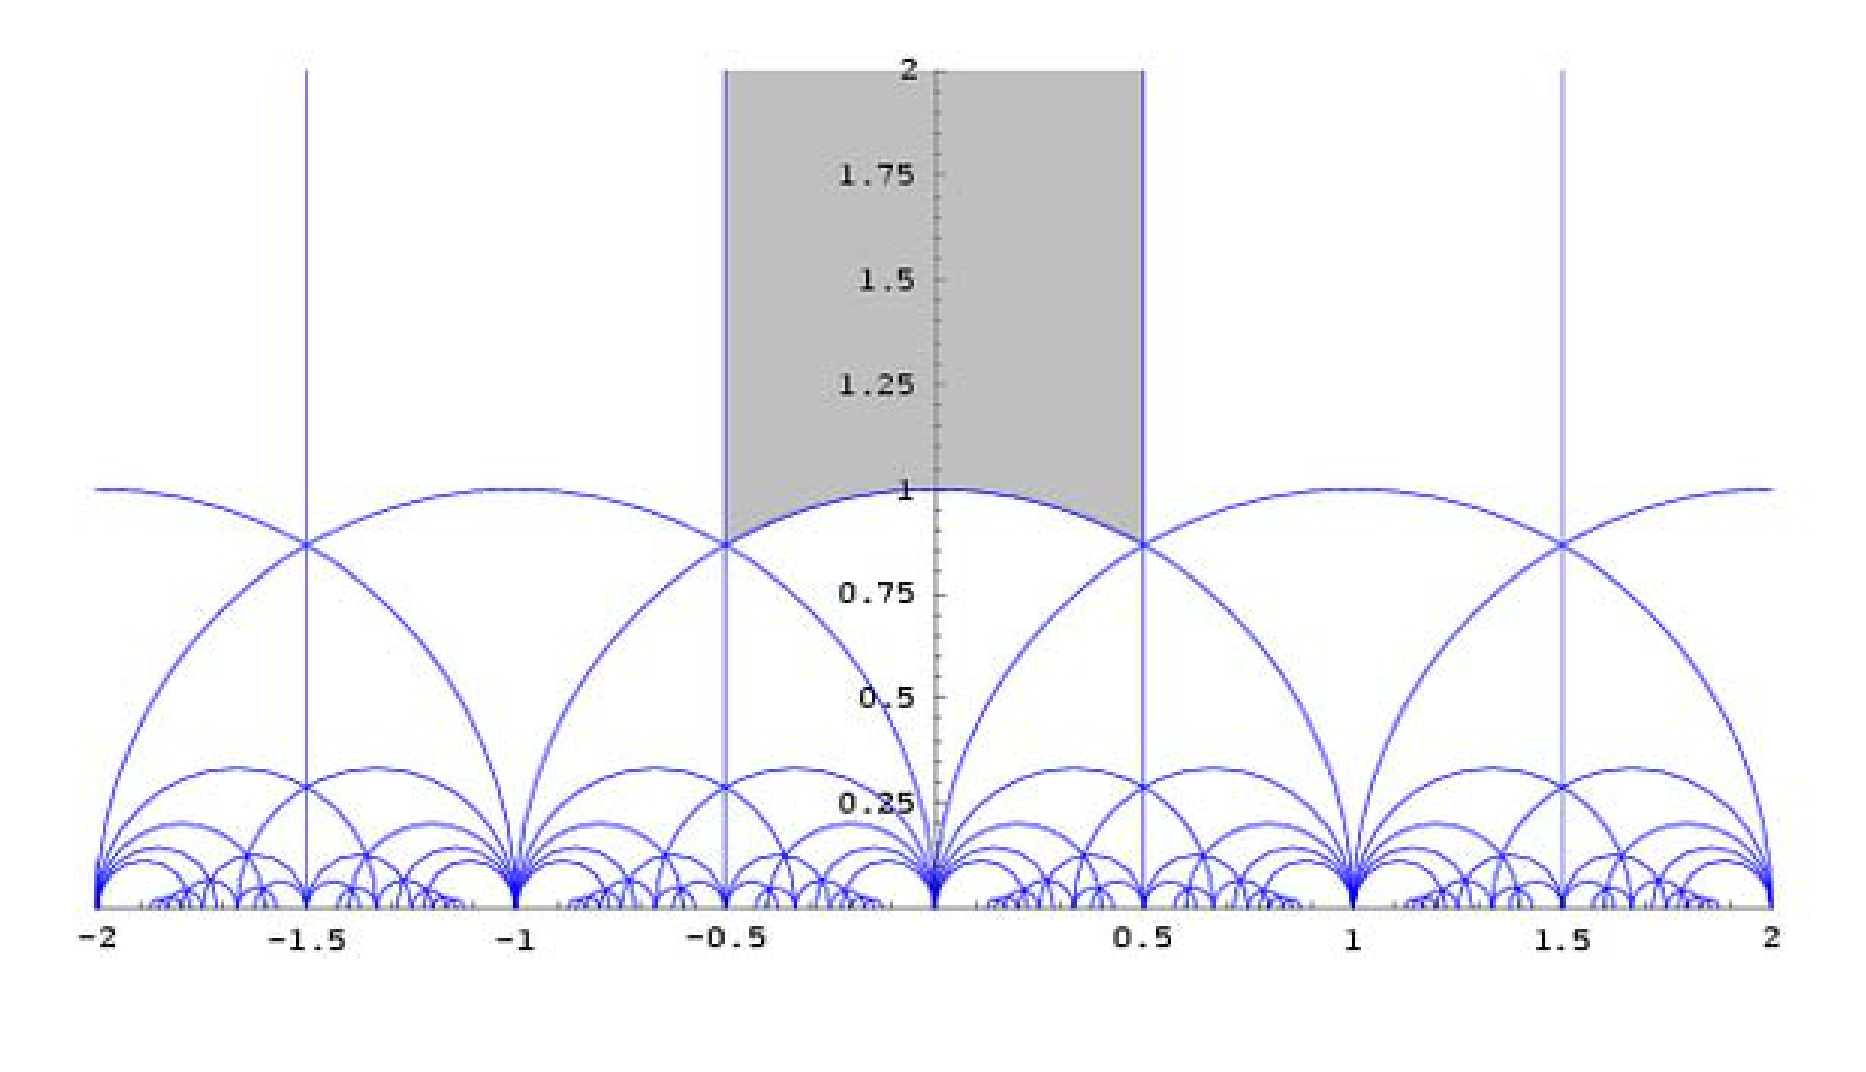
\includegraphics[width=0.78\textwidth]{figures/fig32.png}
  \caption{钥匙孔区域（keyhole region），即 $PSL(2,\mathbb{Z})$ 作用在复上半平面上的标准基本域选择。图取自维基百科「Modular Group」条目。（原文 Fig.~32，第 176 页）}
  \label{fig:32}
\end{figure}

\section{关于 $SL(2,\mathbb{Z})$ 的一些细节} % 原文: C. A Few Details About SL(2, Z)

\begin{keytakeaways}
  \item 模群 $PSL(2,\mathbb{Z}):=SL(2,\mathbb{Z})/\{\pm1\}$ 通过分式线性变换 $\tau\mapsto\frac{a\tau+b}{c\tau+d}$ 有效作用在复上半平面 $\mathcal{H}$ 上；它由 $S=\begin{pmatrix}0&-1\\1&0\end{pmatrix}$ 与 $T=\begin{pmatrix}1&1\\0&1\end{pmatrix}$ 生成。
  \item 关系只有 $S^2=-1$、$(ST)^3=(TS)^3=-1$（及其推论）。$S$ 的符号必须小心：换号后 $(ST)^3$ 变成 $+1$，但 $\bar S\in PSL$ 与符号无关。
  \item 基本域是钥匙孔区域 $\tilde{\mathcal{F}}=\{\tau\in\mathcal{H}:|\tau|\ge1,\ |\operatorname{Re}\tau|\le\frac12\}$（图 32）。证明分两步：引理 1 处理边界上的等距点（核心是配方估计 (C.8)），引理 2 列出三个有非平凡稳定化子的椭圆点 $i,\omega,-\omega^2$。
  \item 构造性算法：对 $(A,C)$ 作辗转相除法得连分数系数 $q_1,\dots,q_{N+1}$，把每步写成矩阵方程 (C.17)--(C.20)，再用 $\sigma^1\sigma^3=S$ 把 $\det\tilde g=(-1)^{N+1}$ 修正为 $SL(2,\mathbb{Z})$ 元素，最终得 $h=g^{-1}T^n$ 的 $S,T$ 字表达 (C.26)--(C.27)。
\end{keytakeaways}

\subsection{生成元与 $PSL(2,\mathbb{Z})$ 的基本域} % 原文: C.1 Generators And A Fundamental Domain For PSL(2, Z)

模群是 $PSL(2,\mathbb{Z}):=SL(2,\mathbb{Z})/\{\pm1\}$，其中 $SL(2,\mathbb{Z})$ 是 $SL(2,\mathbb{R})$ 中所有矩阵元皆为整数的矩阵构成的子群。回忆该群通过
\begin{equation}
  \begin{pmatrix}
    a & b\\
    c & d
  \end{pmatrix}\cdot\tau:=\frac{a\tau+b}{c\tau+d}
  \tag{C.1}
  \label{eq:C.1}
\end{equation}
有效地作用在复上半平面 $\mathcal{H}$ 上。

我们将求出这个群作用的一个基本域，并在此过程中证明 $SL(2,\mathbb{Z})$ 由下面定义的群元 $S$ 与 $T$ 生成：
{\small\itshape ［原文标记：需要检查我们在全文中是否一直使用了自洽的 $S$ 符号约定。］}
% [原文待办标记，原文 p.176 右侧边注]

\begin{equation}
  S=\begin{pmatrix}
    0 & -1\\
    1 & 0
  \end{pmatrix}
  \tag{C.2}
  \label{eq:C.2}
\end{equation}
\begin{equation}
  T=\begin{pmatrix}
    1 & 1\\
    0 & 1
  \end{pmatrix}
  \tag{C.3}
  \label{eq:C.3}
\end{equation}
这些矩阵满足关系
\begin{equation}
  \begin{aligned}
    S^2&=-1\\
    (ST)^3&=(TS)^3=-1
  \end{aligned}
  \tag{C.4}
  \label{eq:C.4}
\end{equation}
% [Tutor Note: 注意 (C.4) 右边是 $-1$ 而非 $1$：这正是取 $S=\begin{pmatrix}0&-1\\1&0\end{pmatrix}$（而非其负号）的结果，也说明 $S,T$ 生成的是 $SL(2,\mathbb{Z})$ 而不是 $PSL(2,\mathbb{Z})$。在下文 (C.9)、(C.10) 里 $(ST)^3=-1$ 会是 $\bar S\bar T$ 阶为 3 的来源。若把 $S$ 换成 $\begin{pmatrix}0&1\\-1&0\end{pmatrix}$，则 (C.4) 变成 $S^2=-1$、$(ST)^3=(TS)^3=+1$，与作者的提醒一致]

注意，若改变 $S$ 的符号，则 $(ST)^3=(TS)^3=+1$，所以对 $S$ 的符号定义要小心一些。

把 $S,T$ 在 $PSL(2,\mathbb{Z})$ 中的像记为 $\bar S,\bar T$。注意 $\bar S$ 不依赖于 $S$ 的符号。\footnote{这里我们沿用 J.-P. Serre，《A Course in Arithmetic》，Springer GTM 7，pp.~78--79 中一个非常好的论证。}

令
\begin{equation}
  \tilde{\mathcal{F}}:=\{\tau\in\mathcal{H}\,|\,|\tau|\ge1\quad\&\quad|\operatorname{Re}(\tau)|\le\tfrac{1}{2}\}
  \tag{C.5}
  \label{eq:C.5}
\end{equation}
这差不多是模群的典范基本域，但还不完全是。它就是图 32 所示的著名的\emph{钥匙孔区域}。令 $\bar G$ 为由 $\bar S$ 与 $\bar T$ 生成的子群。我们断言 $\cup_{g\in\bar G}\,g\cdot\tilde{\mathcal{F}}$ 是整个上半平面。为证明这一点，回忆对任意 $g\in SL(2,\mathbb{Z})$ 有
\begin{equation}
  \operatorname{Im}(g\cdot\tau)=\frac{\operatorname{Im}\tau}{|c\tau+d|^2}
  \tag{C.6}
  \label{eq:C.6}
\end{equation}
现在，对任意固定的 $\tau\in\mathcal{H}$，函数 $|c\tau+d|$ 在 $SL(2,\mathbb{Z})$ 上有下界，从而在 $G$ 上有下界。事实上，把 $\tau=x+iy$ 分成实部与虚部，
\begin{equation}
  |c\tau+d|^2=(cx+d)^2+c^2y^2\ge
  \begin{cases}
    y^2 & c\ne0\\
    d^2\ge1 & c=0
  \end{cases}
  \tag{C.7}
  \label{eq:C.7}
\end{equation}
因此，对任意固定的 $\tau$，必存在群元 $g\in\bar G$，使得 $\operatorname{Im}(g\cdot\tau)$ 作为 $g$ 的函数取极大值。注意用 $\bar T$ 或 $\bar T^{-1}$ 的幂左乘 $g$ 不改变这一性质，所以使 $\operatorname{Im}(g\cdot\tau)$ 极大的 $g$ 并不唯一。我们可以用 $|\operatorname{Re}(g\cdot\tau)|\le\frac{1}{2}$ 来消去这个不确定性。选取这样的群元 $g$。我们断言：对这个变换，$\tau'=g\cdot\tau\in\tilde{\mathcal{F}}$。只需再验证 $|\tau'|\ge1$。否则 $|\tau'|<1$，但此时 $\operatorname{Im}(\bar S\cdot\tau')=\operatorname{Im}(\tau')/|\tau'|^2>\operatorname{Im}(\tau')$，与 $g$ 的定义矛盾。总之，上半平面的每个元素都可被 $\bar G$ 的适当元素带到 $\tilde{\mathcal{F}}$ 中。

现在我们需要两个引理：

\textbf{引理 1：}若 $g\in SL(2,\mathbb{Z})$ 与 $\tau$ 具有如下性质：$\tau\in\tilde{\mathcal{F}}$ 且 $g\cdot\tau\in\tilde{\mathcal{F}}$，则
\begin{enumerate}
  \item $|\operatorname{Re}(\tau)|=\frac{1}{2}$ 且 $g\cdot\tau=\tau\pm1$，或者
  \item $|\tau|=1$
\end{enumerate}

为证明这一点，注意不失一般性（WLOG）可设 $\operatorname{Im}(g\cdot\tau)\ge\operatorname{Im}\tau$。（否则作替换 $g\to g^{-1}$、$\tau\to g^{-1}\tau$。）但这个等式蕴含 $1\ge|c\tau+d|$，后者又蕴含
\begin{equation}
  \begin{aligned}
    1&\ge|c\tau+d|^2\\
    &=(cx+d)^2+c^2y^2\\
    &=c^2|\tau|^2+2cdx+d^2\\
    &\ge c^2|\tau|^2-|cd|+d^2\\
    &=c^2\Big(|\tau|^2-\frac{1}{4}\Big)+\Big(|d|-\frac{1}{2}|c|\Big)^2\\
    &\ge\frac{3}{4}c^2+\Big(|d|-\frac{1}{2}|c|\Big)^2
  \end{aligned}
  \tag{C.8}
  \label{eq:C.8}
\end{equation}

由 \eqref{eq:C.8} 我们得出：

\begin{enumerate}
  \item $(c=0,\,d=\pm1)$ \underline{或} $(c=\pm1,\,d=0,\pm1)$。
  \item 不等式取等号当且仅当 $2cdx=-|cd|$ 且 $|\tau|=1$。
\end{enumerate}

若 $c=0$ 且 $d=\pm1$，则 $g\cdot\tau=\tau\pm1$。此时显然 $|\operatorname{Re}(\tau)|=\frac{1}{2}$。若 $c=\pm1$ 且 $d=0,\pm1$，则不等式取等号，从而 $|\tau|=1$。

\textbf{引理 2：}若 $\tau\in\tilde{\mathcal{F}}$ 且 $\bar g\cdot\tau=\tau$，其中 $\bar g\in PSL(2,\mathbb{Z})$、$\bar g\ne1$，则要么
\begin{enumerate}
  \item $\tau=i$，且稳定化子群为 $\{1,\bar S\}$
  \item $\tau=\omega=e^{2\pi i/3}=-\frac{1}{2}+\frac{\sqrt{3}}{2}i$，且稳定化子群为
  \begin{equation}
    \{1,\bar S\bar T,(\bar S\bar T)^2\}
    \tag{C.9}
    \label{eq:C.9}
  \end{equation}
  \item $\tau=-\omega^2=e^{\pi i/3}=\frac{1}{2}+\frac{\sqrt{3}}{2}i$，且稳定化子群为
  \begin{equation}
    \{1,\bar T\bar S,(\bar T\bar S)^2\}
    \tag{C.10}
    \label{eq:C.10}
  \end{equation}
\end{enumerate}

特别地，对 $\tilde{\mathcal{F}}$ 中所有其余的点 $\tau$，稳定化子群是平凡群。

引理 2 很快由引理 1 推出：若 $g\tau=\tau$，则必属 $c=\pm1$ 的情形。若 $d=0$，则对某个整数 $a$ 有 $a-1/\tau=\tau$。但还必须有 $|\tau|=1$，从而 $a=\tau+\bar\tau$。既然 $a$ 是整数，很快发现要么 $a=0$ 而 $\tau=i$，要么 $a=\pm1$ 而 $\tau=\omega$ 或 $-\omega^2$。若 $d=\pm1$，则由取等条件 $2cdx=-|cd|$ 得 $x=-\frac{1}{2}d/|d|$，从而 $\tau=\omega$ 或 $=-\omega^2$。
% [Tutor Note: 这段把引理 2 归结为「$g\tau=\tau$ 且 $\tau\in\tilde{\mathcal{F}}$ 时只能取 $|c|=1$」。缺的一步是：由 $\tau=g^{-1}\tau$ 得 $c\tau^2+(d-a)\tau-b=0$，$c\ne0$ 时 $1/\tau$ 是整系数二次方程的根，$|\tau|=1$ 给 $a=\tau+\bar\tau\in\mathbb{Z}$；作者直接写「we quickly find」跳过了对 $a\in\{-1,0,1\}$（因 $|\operatorname{Re}\tau|\le\frac12$）的枚举。另外 $d=\pm1$ 时的取等条件 $2cdx=-|cd|$ 与 $|\tau|=1$ 联立才能定出 $x$，单用其一不足以定 $\tau$]

现在终于可以证明：

\textbf{定理：}$SL(2,\mathbb{Z})$ 由 $S$ 与 $T$ 生成。

\textit{证明：}令 $\tau_0$ 位于 $\tilde{\mathcal{F}}$ 的\underline{内部}。任取元素 $g\in SL(2,\mathbb{Z})$、$\bar g\ne1$。则存在元素 $g'\in\bar G$，使得 $g'g\cdot\tau_0\in\tilde{\mathcal{F}}$。而且由引理 1，该元素必在 $\tilde{\mathcal{F}}$ 的内部，从而由引理 2，在 $PSL(2,\mathbb{Z})$ 中 $g'g=1$。因此 $\bar g\in\bar G$，即 $\bar G=PSL(2,\mathbb{Z})$。此外 $S^2=-1$，故 $S$ 与 $T$ 生成 $SL(2,\mathbb{Z})$。$\spadesuit$

\begin{enumerate}
  \item 精确的基本域 $\mathcal{F}$ 必须选得使边界上没有两个不同的点彼此 $G$-相关。例如我们可以取边界中 $\operatorname{Re}(\tau)\ge0$ 的那一部分。

  \item 通过像上面那样研究可能的不动点，可以推出 $S$ 与 $T$ 上\underline{仅有}的关系是：
  \begin{equation}
    S^2=-1\qquad (ST)^3=-1
    \tag{C.11}
    \label{eq:C.11}
  \end{equation}
  （以及由它们推出的一切关系）。

  \item 给定 $g\in SL(2,\mathbb{Z})$，可以这样写出给出 $g$ 的 $S,T$ 词：对 $(a,c)$ 施用辗转相除法，并把那里的标准等式按矩阵解释。见第 1 章第 8 节。

  \item 虽然钥匙孔区域是标准的基本域，但基本域的选择并不唯一。例如，图 32 中所示的任一个像都同样可用（当然这样的区域有无穷多个）。此外，把 $\mathcal{F}\to\mathcal{F}+\epsilon$ 平移一下也仍然得到基本域。

  \item $PSL(2,\mathbb{Z})$ 在 $\mathcal{H}$ 上的作用是真不连续的（properly discontinuous），但并不完全自由。若考虑不包含上述稳定化子群的有限指数子群，则作用将是自由的，商空间将是一个漂亮的 Riemann 曲面。
\end{enumerate}

\subsection{把 $SL(2,\mathbb{Z})$ 的元素写成 $S$ 与 $T$ 的词} % 原文: C.2 Expressing Elements Of SL(2, Z) As Words In S And T

群 $SL(2,\mathbb{Z})$ 由
\begin{equation}
  S:=\begin{pmatrix}
    0 & -1\\
    1 & 0
  \end{pmatrix}
  \qquad\&\qquad
  T:=\begin{pmatrix}
    1 & 1\\
    0 & 1
  \end{pmatrix}
  \tag{C.12}
  \label{eq:C.12}
\end{equation}
生成。

下面是把任意元素
\begin{equation}
  h=\begin{pmatrix}
    A & B\\
    C & D
  \end{pmatrix}\in SL(2,\mathbb{Z})
  \tag{C.13}
  \label{eq:C.13}
\end{equation}
分解为 $S$ 与 $T$ 的词的一个算法。

首先注意下面这个简单的

\textbf{引理} 设 $h\in SL(2,\mathbb{Z})$ 如 \eqref{eq:C.13}。又设 $g\in SL(2,\mathbb{Z})$ 满足：
\begin{equation}
  g\cdot\begin{pmatrix}
    A\\
    C
  \end{pmatrix}=\begin{pmatrix}
    1\\
    0
  \end{pmatrix}
  \tag{C.14}
  \label{eq:C.14}
\end{equation}
那么
\begin{equation}
  gh=T^n
  \tag{C.15}
  \label{eq:C.15}
\end{equation}
其中 $n\in\mathbb{Z}$ 为某个整数。

现在，设 $h$ 满足 $A>C>0$。则 $(A,C)=1$，于是可用辗转相除法定义整数 $q_\ell$，$\ell=1,\dots,N+1$，其中 $N\ge1$，使得
\begin{equation}
  \begin{aligned}
    A&=q_1C+r_1 & 0&<r_1<C\\
    C&=q_2r_1+r_2 & 0&<r_2<r_1\\
    r_1&=q_3r_2+r_3 & 0&<r_3<r_2\\
    &\;\;\vdots & &\;\;\vdots\\
    r_{N-2}&=q_Nr_{N-1}+r_N & 0&<r_N<r_{N-1}\\
    r_{N-1}&=q_{N+1}r_N & &
  \end{aligned}
  \tag{C.16}
  \label{eq:C.16}
\end{equation}
且 $r_N=(A,C)=1$。（注意你可以把 $r_0$ 解释为 $C$，这在 $N=1$ 时是必要的。）现在，{\small\itshape ［原文标记：这里 $N=0$？］}
% [原文待办标记，原文 p.180 右侧边注；原文写作 "N = 0 here?"]
把辗转相除法中的第一行写成矩阵形式：
\begin{equation}
  \begin{pmatrix}
    1 & -q_1\\
    0 & 1
  \end{pmatrix}\begin{pmatrix}
    A\\
    C
  \end{pmatrix}=\begin{pmatrix}
    r_1\\
    C
  \end{pmatrix}
  \tag{C.17}
  \label{eq:C.17}
\end{equation}
我们想要方程具有可以迭代该算法的形式，所以需要较大的整数在上面。因此把恒等式改写成
\begin{equation}
  \sigma^1\begin{pmatrix}
    1 & -q_1\\
    0 & 1
  \end{pmatrix}\begin{pmatrix}
    A\\
    C
  \end{pmatrix}=\begin{pmatrix}
    C\\
    r_1
  \end{pmatrix}
  \tag{C.18}
  \label{eq:C.18}
\end{equation}

现在可以迭代此程序了。于是辗转相除法蕴含矩阵恒等式
\begin{equation}
  \tilde g\begin{pmatrix}
    A\\
    C
  \end{pmatrix}=\begin{pmatrix}
    1\\
    0
  \end{pmatrix}
  \tag{C.19}
  \label{eq:C.19}
\end{equation}
\begin{equation}
  \tilde g=(\sigma^1T^{-q_{N+1}})\cdots(\sigma^1T^{-q_1})
  \tag{C.20}
  \label{eq:C.20}
\end{equation}
现在，要应用引理我们需要 $g$ 属于 $SL(2,\mathbb{Z})$，但
\begin{equation}
  \det\tilde g=(-1)^{N+1}
  \tag{C.21}
  \label{eq:C.21}
\end{equation}
我们可以容易地修改方程以得到所需的元素 $g$。把论证分成两种情形：

\begin{enumerate}
  \item 先设 $N+1=2s$ 为偶数。于是把 $\tilde g$ 的因子两两配对，写出
  \begin{equation}
    \begin{aligned}
      (\sigma^1T^{-q_{2\ell}})(\sigma^1T^{-q_{2\ell-1}})&=(\sigma^1\sigma^3)(\sigma^3T^{-q_{2\ell}}\sigma^3)(\sigma^3\sigma^1)T^{-q_{2\ell-1}}\\
      &=-ST^{q_{2\ell}}ST^{-q_{2\ell-1}}
    \end{aligned}
    \tag{C.22}
    \label{eq:C.22}
  \end{equation}
  % [Tutor Note: (C.22) 的三步：先用 $(\sigma^3)^2=1$ 在中间插入 $\sigma^3\sigma^3$；再用 $\sigma^3T^{-q}\sigma^3=T^{q}$（共轭把 $T$ 的幂取反：$\sigma^3\begin{pmatrix}1&-q\\0&1\end{pmatrix}\sigma^3=\begin{pmatrix}1&q\\0&1\end{pmatrix}$）；最后用 $\sigma^1\sigma^3=S$（严格等式，$\sigma^1\sigma^3=\begin{pmatrix}0&-1\\1&0\end{pmatrix}$ 正是 (C.2) 的 $S$）与 $\sigma^3\sigma^1=-i\sigma^2=-S$。于是 $(\sigma^1T^{-q_{2\ell}})(\sigma^1T^{-q_{2\ell-1}})=\sigma^1T^{-q_{2\ell}}\sigma^1T^{-q_{2\ell-1}}=-ST^{q_{2\ell}}ST^{-q_{2\ell-1}}$，负号来自 $\sigma^3\sigma^1=-S$。核对时若把 $\sigma^3\sigma^1$ 误当成 $\sigma^1\sigma^3$，就会丢掉这个负号]

  其中我们用到了 $\sigma^1\sigma^3=-i\sigma^2=S$。因此我们可以写
  \begin{equation}
    \tilde g=g=(-1)^s\prod_{\ell=1}^{s}\big(ST^{q_{2\ell}}ST^{-q_{2\ell-1}}\big)
    \tag{C.23}
    \label{eq:C.23}
  \end{equation}

  \item 现在设 $N+1=2s+1$ 为奇数。于是把恒等式 \eqref{eq:C.19} 改写为
  \begin{equation}
    \sigma^1\tilde g\begin{pmatrix}
      A\\
      C
    \end{pmatrix}=\begin{pmatrix}
      1\\
      0
    \end{pmatrix}
    \tag{C.24}
    \label{eq:C.24}
  \end{equation}
  于是现在只需取
  \begin{equation}
    g=\sigma^1\tilde g=(-1)^{s+1}(ST^{-q_{2s+1}})\prod_{\ell=1}^{s}\big(ST^{q_{2\ell}}ST^{-q_{2\ell-1}}\big)
    \tag{C.25}
    \label{eq:C.25}
  \end{equation}
\end{enumerate}

因此两种情形可以统一表述为
\begin{equation}
  g=(-1)^{\lfloor\frac{N+1}{2}\rfloor}\prod_{\ell=1}^{N+1}\big(ST^{(-1)^\ell q_\ell}\big)
  \tag{C.26}
  \label{eq:C.26}
\end{equation}
% [Tutor Note: (C.26) 与 (C.23)、(C.25) 的符号核对：$N+1=2s$（偶）时 $\lfloor\frac{N+1}{2}\rfloor=s$，与 (C.23) 的 $(-1)^s$ 一致；但 $N+1=2s+1$（奇）时 $\lfloor\frac{N+1}{2}\rfloor=s$，而 (C.25) 给出的是 $(-1)^{s+1}$——两者相差一个整体符号。原文 (C.26) 照印如此，此处照原样转写未改。由于 $-1=S^2$ 是 $SL(2,\mathbb{Z})$ 的中心元，这个整体符号不改变 $h=g^{-1}T^n$ 在 $PSL(2,\mathbb{Z})$ 中的分解，但若要求 $h\in SL(2,\mathbb{Z})$ 逐元素相等，须重核这一步（疑为原稿笔误，或 (C.25) 的 $s+1$ 应为 $s$）。另外 (C.20)、(C.23)、(C.25) 中乘积的书写次序是从 $q_{N+1}$ 在左、$q_1$ 在右，读 $\prod_{\ell=1}^{N+1}$ 时须按同一约定理解]

然后我们终于可以把
\begin{equation}
  h=\begin{pmatrix}
    A & B\\
    C & D
  \end{pmatrix}=g^{-1}T^n
  \tag{C.27}
  \label{eq:C.27}
\end{equation}
写成 $S$ 与 $T$ 的词，其中 $n$ 为适当的整数。（注意 $S^2=-1$。）
{\small\itshape ［原文标记：最好给出确定 $n$ 的算法。］}
% [原文待办标记，原文 p.181 右侧边注；原文写作 "It would be good to give an algorithm for determining n."]

现在需要说明如何把一般的 $h\in SL(2,\mathbb{Z})$ 化成 $A>C>0$ 的形式，以便套用上面的公式。注意
\begin{equation}
  \begin{pmatrix}
    1 & 0\\
    m & 1
  \end{pmatrix}\begin{pmatrix}
    A & B\\
    C & D
  \end{pmatrix}=\begin{pmatrix}
    A & B\\
    C+mA & D+mB
  \end{pmatrix}
  \tag{C.28}
  \label{eq:C.28}
\end{equation}
% [Tutor Note: 原稿 (C.28) 右端矩阵的排版有缺陷：两个元素 $A$、$B$ 之间以及与 $C+mA$、$D+mB$ 之间的列分隔丢失，看起来像 $2\times2$ 矩阵里挤了「$A\ B$」「$C+mA\ D+mB$」两团。按左乘矩阵的含义，它应当是 $\begin{pmatrix}A&B\\C+mA&D+mB\end{pmatrix}$；这里按数学含义排出，特此说明]
而
\begin{equation}
  \begin{pmatrix}
    1 & 0\\
    -m & 1
  \end{pmatrix}=ST^mS^{-1}
  \tag{C.29}
  \label{eq:C.29}
\end{equation}
于是，若 $A>0$，我们可用这一操作平移 $C$，使 $0\le C<A$。若 $A<0$，可乘以 $S^2=-1$ 化到 $A>0$ 的情形。最后，若 $A=0$，则
\begin{equation}
  h=\begin{pmatrix}
    0 & \pm1\\
    \mp1 & n
  \end{pmatrix}
  \tag{C.30}
  \label{eq:C.30}
\end{equation}
而我们写
\begin{equation}
  ST^n=\begin{pmatrix}
    0 & -1\\
    1 & n
  \end{pmatrix}
  \tag{C.31}
  \label{eq:C.31}
\end{equation}
{\small\itshape ［原文标记：需要以一种更有用的方式把结果总结一下。］}
% [原文待办标记，原文 p.181 右侧边注；原文写作 "Need to summarize the result in a useful way"]

% =====================================================================
%  c23 —— 原文印刷页 182--191（PDF 第 183--192 页）
%  含：附录 D（D. Level k Theta Functions；D.1 定义、D.2 模变换律）
%      附录 E（E. Theta Functions And Holomorphic Line Bundles On Tori；
%      E.1 Heisenberg 群作为主 U(1) 丛、E.2 自然联络、
%      E.3 辛环面上的复结构、E.4 拉格朗日分解、
%      E.5 环面上复结构的空间：Siegel 上半平面）
%  编号公式：D.1--D.21、E.1--E.45 共 66 条；本片段无插图。
%  全部公式均逐条对照 150 dpi 页面图像转写（文本层仅供读散文）。
% =====================================================================

\section{第 $k$ 级 theta 函数} % 原文: D. Level k Theta Functions

\begin{keytakeaways}
  \item 定义：第 $k$ 级 theta 函数 $\Theta_{\mu,\kappa}(z,\tau)$ 是 $q^{\ell^2/(4\kappa)}y^{\ell}$
    在 $\ell\equiv\mu\ (\mathrm{mod}\ 2\kappa)$ 上的求和；$\mu$ 只需看成 $\mathbb{Z}/2\kappa\mathbb{Z}$
    的元素，因而同一模类只给出一个函数。
  \item 拟周期性：沿 $z\mapsto z+\nu$ 严格不变，沿 $z\mapsto z+\nu\tau$ 则多出乘性因子
    $e^{-2\pi i\kappa\nu^2\tau-4\pi i\kappa\nu z}$；该因子与 $\mu$ 无关，故所有模类「以同一方式」变换。
  \item 模变换：把 $\Theta_{\mu,\kappa}$ 除以 $\eta(\tau)$ 得到 $f_{\mu,k}$，其张成空间 $V_k$ 是
    $SL(2,\mathbb{Z})$（而非 $PSL(2,\mathbb{Z})$）的表示；按 $-1$ 的本征值分解为
    $\dim V_k^+=k+1$、$\dim V_k^-=k-1$ 的两块。
  \item 生成元的矩阵元：$\rho(S)_{\mu\nu}=\frac{1}{\sqrt{2k}}e^{2\pi i\mu\nu/(2k)}$ 是 Gauss 和型相位，
    $\rho(T)$ 的相位 $\mu^2/(4k)-1/24$ 中的 $-1/24$ 正是中心荷为 $1$ 的 $\eta$ 因子的残留。
  \item 一般元素的变换律 (D.16) 需要两个数论输入：Rademacher 函数 $\Phi(A)$（由 Dedekind 和给出，
    取整值）与连分数项数 $t$（只在模 $2$ 意义下良定义，故 $(-1)^t$ 良定义）。
\end{keytakeaways}

\subsection{定义} % 原文: D.1 Definition

这里汇集关于 theta 函数的若干事实。回忆
\begin{equation}
\begin{aligned}
  \Theta_{\mu,\kappa}(z,\tau) &:= \sum_{\ell=\mu\,\mathrm{mod}\,2\kappa} q^{\ell^2/(4\kappa)} y^{\ell}\\
  &= \sum_{n\in\mathbb{Z}} q^{\kappa(n+\mu/(2\kappa))^2} y^{(\mu+2\kappa n)}\\
  &= \sum_{n\in\mathbb{Z}} e^{i\pi\tau(2\kappa)(n+\mu/(2\kappa))^2+2\pi i(2\kappa)z(n+\mu/(2\kappa))}
\end{aligned}
\tag{D.1}
\label{eq:D.1}
\end{equation}
其中 $q=e^{2\pi i\tau}$，$y=e^{2\pi iz}$。这里 $\mu$ 是整数，$\kappa$ 是正半整数（即属于
$\frac12\mathbb{Z}_+$）。注意若把 $\mu$ 平移为 $\mu\to\mu+2\kappa s$，$s$ 为任意整数，则
$\Theta_{\mu,\kappa}$ 不变。人们常把 $\mu$ 取在基本域 $-\kappa<\mu\le\kappa$ 内，但一般说来应当把
$\mu$ 视为 $\mathbb{Z}/2\kappa\mathbb{Z}$ 的元素。作为 $z$ 的函数，这些函数是双拟周期的：
\begin{equation}
\begin{aligned}
  \Theta_{\mu,\kappa}(z+\nu,\tau) &= \Theta_{\mu,\kappa}(z,\tau)\\
  \Theta_{\mu,\kappa}(z+\nu\tau,\tau) &= e^{-2\pi i\kappa\nu^2\tau-4\pi i\kappa\nu z}\Theta_{\mu,\kappa}(z,\tau)
\end{aligned}
\tag{D.2}
\label{eq:D.2}
\end{equation}
这里 $\nu$ 是任意整数。注意对一切 $\mu\in\mathbb{Z}/2\kappa\mathbb{Z}$，theta 函数的变换方式都相同。
关于这些 theta 函数的几何意义，我们将在下文的
{\small\itshape ［原文标记：section ****（章节号待补，原稿占位符）］} 中作更多解释。
% [原文待办标记，原文 p.182：正文写的是「in section **** below」，星号是作者留给自己的章节号占位符]

% [Tutor Note: (D.1) 三行是同一个求和的三种写法，核对时最易错的是指数。第一行的 $\ell$ 跑遍与
% $\mu$ 同余模 $2\kappa$ 的整数，故 $\ell^2/(4\kappa)$ 与第二行的 $\kappa(n+\mu/(2\kappa))^2$ 相等
% 只须代入 $\ell=\mu+2\kappa n$：$(2\kappa)^2/(4\kappa)=\kappa$，这正是「$4\kappa=(2\kappa)^2/\kappa$」
% 那一步。第三行把 $q=e^{2\pi i\tau}$、$y=e^{2\pi iz}$ 代回，于是 $\tau$ 前多出因子 $2\kappa$、
% $z$ 前也多出因子 $2\kappa$——这两处因子最容易漏掉其中一个。]

\subsection{第 $k$ 级 theta 函数的模变换律} % 原文: D.2 Modular Transformation Laws For Level k Theta Functions
{\small\itshape ［原文标记：此处需要把约定 $k$ 改成 $\kappa$］}
% [原文待办标记，原文 p.182 右侧页边注：\ensuremath{\clubsuit} Need to change conventions k → κ here \ensuremath{\clubsuit}]

实际上，用下面这些函数来工作会更方便：
\begin{equation}
  f_{\mu,k}(z,\tau) := \frac{\Theta_{\mu,k}(z,\tau)}{\eta(\tau)}
  \tag{D.3}
  \label{eq:D.3}
\end{equation}
把这些函数的张成（span）记作 $V_k$。它将是 $SL(2,\mathbb{Z})$ 的一个表示（而\emph{不是}
$PSL(2,\mathbb{Z})$ 的表示），我们的目标就是确定这个表示。对应于 $-1\in SL(2,\mathbb{Z})$ 的作用的
对合 $z\to -z$ 可以对角化，从而把 $V_k$ 分解为偶子空间与奇子空间的直和
\begin{equation}
  V_k\cong V_k^+\oplus V_k^-
  \tag{D.4}
  \label{eq:D.4}
\end{equation}
于是 $\dim V_k^+=k+1$，$\dim V_k^-=k-1$。奇空间 $V_k^-$ 中一般第 $k$ 级 theta 函数的变换规则，
是 Lisa Jeffrey [31] 在一项令人印象深刻的计算中导出的。借助她论文中的想法，可以把结果推广为
$V_k$ 中全部 theta 函数的变换律。这个计算略有些非平凡，所以此处直接给出结果（因为它在别处似乎
还查不到）。

我们在 $(z,\tau)$ 上有一个 $SL(2,\mathbb{Z})$ 的\emph{左}作用：若
\begin{equation}
  A = \begin{pmatrix} a & b\\ c & d\end{pmatrix}
  \tag{D.5}
  \label{eq:D.5}
\end{equation}
则
\begin{equation}
  A\cdot(z,\tau) := \left(\frac{z}{c\tau+d},\ \frac{a\tau+b}{c\tau+d}\right)
  \tag{D.6}
  \label{eq:D.6}
\end{equation}
定义
\begin{equation}
  \phi_k(A;(z,\tau)) = \exp 2\pi i k\,\frac{cz^2}{c\tau+d}
  \tag{D.7}
  \label{eq:D.7}
\end{equation}
那么
\begin{equation}
  \phi_k(A_1;A_2\cdot(z,\tau))\,\phi_k(A_2;(z,\tau)) = \phi_k(A_1A_2;(z,\tau))
  \tag{D.8}
  \label{eq:D.8}
\end{equation}
现在在 $V_k$ 上定义一个\emph{左}作用 $SL(2,\mathbb{Z})$：
\begin{equation}
  (\rho(A)\cdot f)(z,\tau) := \left(\phi_k(A^{-1};(z,\tau))\right)^{-1} f(A^{-1}\cdot(z,\tau))
  \tag{D.9}
  \label{eq:D.9}
\end{equation}
于是，相对于基 $f_{\mu,k}$，我们有
\begin{equation}
  \rho(A)\cdot f_{\mu,m} := \sum_{\nu}\rho(A)_{\nu\mu}f_{\nu}
  \tag{D.10}
  \label{eq:D.10}
\end{equation}
其中再次把 $\mu,\nu$ 视为模 $2k$ 的整数。

若 $a=0$，则 $A=S$ 或 $S^{-1}$，其中我们定义
\begin{equation}
  S := \begin{pmatrix} 0 & -1\\ 1 & 0\end{pmatrix}
  \tag{D.11}
  \label{eq:D.11}
\end{equation}
若 $c=0$ 且 $a=1$，则 $A=T^m$，此时只须算出
\begin{equation}
  T := \begin{pmatrix} 1 & 1\\ 0 & 1\end{pmatrix}
  \tag{D.12}
  \label{eq:D.12}
\end{equation}
的矩阵就够了。

若 $c=0$ 且 $a=-1$，则只须算出 $A=-1$ 的作用。直接计算给出：
\begin{equation}
  \rho(-1)_{\mu\nu} = \delta_{\mu+\nu,0}
  \tag{D.13}
  \label{eq:D.13}
\end{equation}
这就是电荷共轭矩阵。
\begin{equation}
  \rho(S)_{\mu\nu} = \frac{1}{\sqrt{2k}}\exp\left(2\pi i\,\frac{\mu\nu}{2k}\right)
  \tag{D.14}
  \label{eq:D.14}
\end{equation}
\begin{equation}
  \rho(T)_{\mu\nu} = \delta_{\mu,\nu}\exp\left(2\pi i\left[\frac{\mu^2}{4k}-\frac{1}{24}\right]\right)
  \tag{D.15}
  \label{eq:D.15}
\end{equation}
若 $ac\ne 0$，则
\begin{equation}
  \rho(A)_{\mu\nu} = \frac{1}{\sqrt{2k|c|}}
  e^{\frac{i\pi}{2k}\frac{b}{a}\nu^2}
  e^{-\frac{2\pi i}{24}\Phi(A)}
  \sum_{\gamma\,\mathrm{mod}(2kc),\ \gamma=\mu\,\mathrm{mod}\,2k}
  \exp\left[i\pi\frac{a}{2kc}\left(\gamma+(-1)^{t+1}\frac{\nu}{a}\right)^2\right]
  \tag{D.16}
  \label{eq:D.16}
\end{equation}
这里 $\Phi(A)$ 是 Rademacher 函数，$t$ 是 $A$ 的任一连分数展开中的项数。虽然 $A$ 可以容许许多种
连分数展开，我们断言项数模 $2$ 是良定义的，因此 $(-1)^t$ 是 $A$ 的良定义函数。

% [Tutor Note: (D.10) 与 (D.13)--(D.16) 的指标次序不同，极易混淆。(D.10) 里写的是
% $\rho(A)_{\nu\mu}$，即第一个下标是行、第二个下标是列，而 $\sum_\nu$ 收缩的是列指标，这正是
% 「左作用」的样子；(D.13)--(D.16) 则直接给出矩阵元 $\rho(A)_{\mu\nu}$，两者相差一次转置。
% 若照抄时把 (D.10) 也写成 $\rho(A)_{\mu\nu}$，后面 (D.17) 的检验（$\gamma\to-\gamma$ 换元）就会
% 给出错误的对称性；另外 (D.10) 里基函数的下标原作 $f_{\mu,m}$，与全片的 $f_{\mu,k}$ 不一致，
% 疑为笔误，此处照原样转写。]

% [Tutor Note: (D.16) 的两处相位要分开看：$e^{-\frac{2\pi i}{24}\Phi(A)}$ 与 (D.15) 里方括号中的
% $-1/24$ 同源，都来自 $\Theta/\eta$ 中 $\eta(\tau)$ 的中心荷 $c=1$ 相位（$e^{2\pi i/24}$ 的十二次
% 幂为 $1$，故它只在模 $24$ 意义下确定）；而 $e^{\frac{i\pi}{2k}\frac{b}{a}\nu^2}$ 则是
% 「$b/a$ 型」二次相位的高斯和。核对 (D.16) 的关键是：把 $A=S$（$a=0$）代入会发散，所以 (D.16)
% 只在 $ac\ne0$ 时成立，$a=0$ 与 $c=0$ 分别由 (D.14)、(D.15) 单独给出。$(-1)^{t+1}$ 中的 $t$
% 必须取自同一次连分数展开，因为 $t$ 本身只在模 $2$ 下良定义——这一点正是下一段所强调的。]

（见 {\small\itshape ［原文标记：section ??（交叉引用的章节号未定）］}。）正是这个符号构成了与
Lisa Jeffrey 就奇 theta 函数所得表达式之间最重要的差别。
% [原文待办标记，原文 p.184：正文写的是「(See section ??.)」，问号是未定的 \ref 占位符]

注意
\begin{equation}
  \rho(A)_{\mu,\nu} = \rho(A)_{-\mu,-\nu}
  \tag{D.17}
  \label{eq:D.17}
\end{equation}
对一切 $A\in SL(2,\mathbb{Z})$ 成立。这必定如此，因为代表 $-1$ 的电荷共轭必须与所有矩阵对易。
就 (D.16) 的情形而言，这也可以通过把求和变量改为 $\gamma\to-\gamma$ 来验证。

剩下要定义的就是 $t$ 与 Rademacher 函数。

Rademacher 函数的定义与 [31] 中完全一样。函数 $\Phi:SL(2,\mathbb{Z})\to\mathbb{Z}$ 由下式定义
\begin{equation}
  \Phi(A) :=
  \begin{cases}
    \dfrac{a+d}{c}-12\operatorname{sign}(c)\,s(d,|c|) & c\ne 0\\[2mm]
    \dfrac{b}{d} & c=0
  \end{cases}
  \tag{D.18}
  \label{eq:D.18}
\end{equation}
其中 $s(d,c)$ 是 Dedekind 和，对 $c>0$ 定义为
\begin{equation}
  s(d,c) = \frac{1}{4c}\sum_{k=1}^{c-1}\cot\frac{\pi k}{c}\cot\frac{\pi dk}{c}
  \tag{D.19}
  \label{eq:D.19}
\end{equation}
（当 $d\ne 0$），并约定 $s(0,1)=0$。$\Phi$ 取整值这一点远非显然，但它可由下面这个值得注意的公式
推出
\begin{equation}
  \Phi(A_{12}) = \Phi(A_1)+\Phi(A_2)-3\operatorname{sign}(c_1c_2c_{12})
  \tag{D.20}
  \label{eq:D.20}
\end{equation}
其中 $A_{12}=A_1A_2$。

利用连分数理论可以证明，任何 $A\in SL(2,\mathbb{Z})$ 都具有如下形式
\begin{equation}
  A = T^{m_t}ST^{m_{t-1}}S\cdots T^{m_1}S
  \tag{D.21}
  \label{eq:D.21}
\end{equation}
其中——这一点很重要——所有 $m_i\ne 0$。由于群中的关系式，整数 $t$ 只在模 $2$ 意义下良定义。

% [Tutor Note: 作者写「$\Phi$ 取整值……远非显然」，跳过的是 Dedekind 和的三项关系
% （Dedekind reciprocity）：正是这条经典互反公式保证 (D.20) 中的组合在 $A_{12}=A_1A_2$ 处取整值，
% 进而由一个归纳论证给出 $\Phi(A)\in\mathbb{Z}$。要补齐这一步，可查 Rademacher 关于 Dedekind 和的
% 原始工作，或 Zagier 关于 Dedekind 和互反公式的综述；[31] 中只按定义引用而未复述证明。]

\section{环面上的 theta 函数与全纯线丛} % 原文: E. Theta Functions And Holomorphic Line Bundles On Tori

\begin{keytakeaways}
  \item 统一的视角：环面上的 theta 函数是某个主 $U(1)$ 丛（Heisenberg 群的中心扩张）的全纯截面，
    而模变换律来自丛的构造本身，与截面的具体选法无关。
  \item Heisenberg 群：整值辛形式 $\Omega:\Lambda\times\Lambda\to\mathbb{Z}$ 诱导中心扩张
    $0\to U(1)\to\tilde V\to V\to 0$；在 $\Lambda$ 上取分裂 $\epsilon$ 后商掉 $\Lambda_\epsilon$，
    即得环面上的主 $U(1)$ 丛 $(V\times U(1))/\Lambda$，其量子化维度为 $\dim\mathcal{H}=e_1\cdots e_n$，
    相应的线丛就是预量子线丛。
  \item 自然联络：平行移动由 $V$ 中的平移给出，曲率恰为 $\Omega$；第一 Chern 类由
    $(e_1,\dots,e_n)\in H^2(V/\Lambda;\mathbb{Z})$ 给出，闭路的和乐为
    $e^{2\pi i\Omega(\lambda,w_0)}\epsilon_\lambda^{-1}$。
  \item 复结构：取与 $\Omega$ 相容的 $J$，则 $g(v,w)=\Omega(Jv,w)$ 对称；周期矩阵
    $\tau_{IJ}$ 落在 Siegel 上半平面 $\mathcal{H}_N$ 内，且 $\mathcal{H}_N\cong Sp(2N,\mathbb{R})/U(N)$。
  \item 模空间：$\mathbb{R}^{2N}/\mathbb{Z}^{2N}$ 上复结构的空间是
    $Sp(2N,\mathbb{Z})\backslash\mathcal{H}_N$；$Sp(2N,\mathbb{Z})$ 由三类生成元给出，这正是 theta
    函数具有如此模变换性质的根源。
\end{keytakeaways}

在处理阿贝尔 Chern-Simons 理论时，对 theta 函数及其与环面上线丛截面的关系有一个一般的看法是很有用的。
这里把这套理论概述一遍。

若干数学处理可参见

\begin{enumerate}
  \item D. Mumford，\textit{Tata Lectures on Theta}，第 I 卷，p.202。那里对 theta 函数的变换
    有很好的描述。
  \item D. Mumford、M. Nori 与 P. Norman，\textit{Tata Lectures on Theta}，第 III 卷。他们把
    $\theta$ 解释为 Fock 空间表示中的一个特殊向量，也把 $\theta$ 解释为 Heisenberg 表示中的一个
    特殊矩阵元。
  \item 在代数几何框架内的另一种很好的描述可见 Griffiths 与 Harris，p.300 及其后。
  \item 专门讨论这一主题的一本很好的书是 Birkenhake 与 Lange，
  \item 这一主题在数以百计的物理学论文中从各种观点被处理过。我们用到了 [9] 的 pp.68--69 以及
    [20] 的第 6 节。
\end{enumerate}

\subsection{作为主 $U(1)$ 丛的 Heisenberg 群} % 原文: E.1 Heisenberg Groups As Principal U(1) Bundles

假设 $\Lambda$ 是一个秩为 $2n$ 的格，其上有整值辛形式：
\begin{equation}
  \Omega:\Lambda\times\Lambda\to\mathbb{Z}
  \tag{E.1}
  \label{eq:E.1}
\end{equation}
它诱导出实 $2n$ 维向量空间 $V=\Lambda\otimes\mathbb{R}$ 上的辛形式。利用 $\Omega$ 我们定义一个中心扩张
\begin{equation}
  0\to U(1)\to\tilde V\to V\to 0.
  \tag{E.2}
  \label{eq:E.2}
\end{equation}
可以把 $\tilde V$ 看成数对 $(v,z)\in V\times U(1)$ 的集合，其乘法由一个上闭链（cocycle）给出
\begin{equation}
  (v,z)(v',z') = (v+v',zz'c(v,v'))
  \tag{E.3}
  \label{eq:E.3}
\end{equation}
使得
\begin{equation}
  \frac{c(v,v')}{c(v',v)} = e^{2\pi i\Omega(v,v')}.
  \tag{E.4}
  \label{eq:E.4}
\end{equation}
{\small\itshape ［原文标记：若把约定改一改会更好，即把中心部分放在第一个因子上，于是元素写成
$(z,v)$ 而不是 $(v,z)$。这在接下来的全篇中都需要改。］}
% [原文待办标记，原文 p.185 右侧页边注：\ensuremath{\clubsuit} Would be better to change convention and put the central
% part as the first factor, so write elements as (z,v) rather than (v,z). That needs to be changed
% throughout the following. \ensuremath{\clubsuit}]

自然地取 $c(v,v')=e^{i\pi\Omega(v,v')}$，它对应于主 $U(1)$ 丛 $\tilde V\to V$ 的一个特殊平凡化。

现在可以构造环面 $V/\Lambda$ 上的主 $U(1)$ 丛了。为此我们把序列 (E.2) 在 $\Lambda$ 上分裂。也就是说，
选取一个函数 $\epsilon:\Lambda\to U(1)$，满足
\begin{equation}
  \epsilon_v\epsilon_{v'} = e^{-i\pi\Omega(v,v')}\epsilon_{v+v'}\qquad \forall v,v'\in\Lambda
  \tag{E.5}
  \label{eq:E.5}
\end{equation}
{\small\itshape ［原文标记：需要解释这样的分裂为何存在。］}
% [原文待办标记，原文 p.185 右侧页边注：\ensuremath{\clubsuit} Explain why such a splitting exists. \ensuremath{\clubsuit}]

现在 (E.5) 正是我们所需要的条件，使得 $v\to(v,\epsilon_v)$ 定义出同态 $\Lambda\to\tilde V$，即把
$\Lambda$ 嵌入群 $\tilde V$ 中。

把这个同态的像记作 $\Lambda_\epsilon$。现在取商 $\tilde V/\Lambda_\epsilon$ 就有意义了。这个空间是
$V/\Lambda$ 上的一个主 $U(1)$ 丛。

作为空间，我们的 $U(1)$ 丛可以写成 $(V\times U(1))/\Lambda$，其中的等价关系是
\begin{equation}
  (v,z)\sim(v,z)\cdot(\lambda,\epsilon_\lambda) = (v+\lambda,\epsilon_\lambda e^{i\pi\Omega(v,\lambda)}\cdot z)
  \tag{E.6}
  \label{eq:E.6}
\end{equation}

% [Tutor Note: 作者在 (E.5) 后让我们「相信分裂存在」，其实这一步可以显式写出：因 $\Omega$ 在
% $\Lambda$ 上取整值，$\Omega(\lambda,\lambda)\in\mathbb{Z}$，故 $\epsilon_\lambda:=e^{i\pi\Omega(\lambda,\lambda)/2}$
% 取值只可能是 $\pm1$，把它代入 (E.5) 并利用 $\Omega(v+v',v+v')=\Omega(v,v)+\Omega(v',v')+2\Omega(v,v')$
% 即得 $\epsilon_v\epsilon_{v'}\epsilon_{v+v'}^{-1}=e^{-i\pi\Omega(v,v')}$，条件恰好成立。也就是说，
% 「分裂存在」等价于 $\Omega$ 的整性；若 $\Omega$ 只是实值的，还可以差一个特征标，这正对应
% 下面第 2 条注记中的「二次细化」。]

\paragraph{注记}
\begin{enumerate}
  \item 在上述扩张中 $z\in U(1)$，所以我们构造的是主 $U(1)$ 丛。用这样的描述很容易得到相应的
    相伴丛。下文要描述环面上的全纯丛，届时这一点会很重要。只要在上述各式中让 $z$ 取值于
    $\mathbb{C}^*$ 或 $\mathbb{C}$，我们就能直接定义相伴的 $\mathbb{C}^*$ 或 $\mathbb{C}$ 丛！
    用 $\mathbb{C}^*$ 作的扩张会收缩到用 $U(1)$ 作的扩张上。
    {\small\itshape ［原文标记：这第一条注记位置不当，或者根本不必要。］}
    % [原文待办标记，原文 p.187 右侧页边注：\ensuremath{\clubsuit} This first remark is out of place or just not necessary. \ensuremath{\clubsuit}]
  \item 由于 $\Omega$ 在 $\Lambda\times\Lambda$ 上整值，双线性形式 $e^{i\pi\Omega(v,v')}$ 实际上是对称
    双线性形式。一般地，给定阿贝尔群 $A$ 上的对称形式
    \begin{equation}
      b:A\times A\to\mathbb{R}/\mathbb{Z}
      \tag{E.7}
      \label{eq:E.7}
    \end{equation}
    $b$ 的一个\emph{二次细化}（quadratic refinement）是函数 $q:A\to\mathbb{R}/\mathbb{Z}$，满足
    \begin{equation}
      q(x+y)-q(x)-q(y)+q(0)=b(x,y)
      \tag{E.8}
      \label{eq:E.8}
    \end{equation}
    注意我们可以把 $\epsilon$ 看作这个对称……
    （原文此处断句，句子在此中断；所缺的宾语即「对称形式 $b$ 的二次细化」，
    把 (E.5) 取对数并与 (E.8) 对照即可看出）
  \item 这给出了\emph{紧相空间}的一个漂亮例子。$T(V/\Lambda)$ 是辛流形。这类相空间的量子化应当
    给出一个有限维 Hilbert 空间，而在 WKB 近似下其维数应当是
    \begin{equation}
      \dim\mathcal{H} = \int_T\frac{\Omega^n}{n!}
      \tag{E.9}
      \label{eq:E.9}
    \end{equation}
    现在，$\Lambda$ 上任一整值反对称形式都可以看成一个矩阵，而在格的基变换
    $\Omega\to A^{tr}\Omega A$（$A\in GL(2n,\mathbb{Z})$）之下，我们可以把 $\Omega$ 化成如下形式：
    \begin{equation}
      \Omega = -ie_1\sigma^2\oplus -ie_2\sigma^2\oplus\cdots
      \tag{E.10}
      \label{eq:E.10}
    \end{equation}
    {\small\itshape ［原文标记：请给出证明。］}
    % [原文待办标记，原文 p.187 右侧页边注：\ensuremath{\clubsuit} Indicate the proof \ensuremath{\clubsuit}]
    其中 $e_I$，$I=1,\dots,n$ 是整数。我们可以要求 $e_1|e_2|\cdots|e_n$ 来把它们唯一确定。这就定义
    了所谓的\emph{辛基}。这一点后文还会再谈。此时 $\dim\mathcal{H}=e_1\cdots e_n$。在几何量子化中，
    与我们 $U(1)$ 丛相伴的线丛就是预量子线丛（pre-quantum line bundle）。
\end{enumerate}

\paragraph{练习}
说明主 $U(1)$ 丛还可以有如下另一种表示。由上闭链 $c((x,y),(x',y'))=xy'$ 构造 Heisenberg 表示
\begin{equation}
  0\to\mathbb{R}\to Heis(\mathbb{R}\times\mathbb{R})\to\mathbb{R}\times\mathbb{R}\to 0
  \tag{E.11}
  \label{eq:E.11}
\end{equation}
它有一个漂亮的 $3\times 3$ 矩阵表示
\begin{equation}
  \begin{pmatrix} 1 & x & z\\ 0 & 1 & y\\ 0 & 0 & 1\end{pmatrix}
  \tag{E.12}
  \label{eq:E.12}
\end{equation}
从拓扑上说这不过是 $\mathbb{R}^3$，但群乘法是非交换的。注意
\begin{equation}
  0\to\mathbb{Z}\to Heis(\mathbb{Z}\times\mathbb{Z})\to\mathbb{Z}\times\mathbb{Z}\to 0
  \tag{E.13}
  \label{eq:E.13}
\end{equation}
构成一个离散子群，只要取 $x,y,z$ 为整数即可。于是把 $\mathbb{R}^3/\mathbb{Z}^3$ 实现为
$Heis(\mathbb{R}\times\mathbb{R})/Heis(\mathbb{Z}\times\mathbb{Z})$ 时，它是环面上的一个 $U(1)$ 丛。

在关于弦紧化的文献中，这被称为「扭环面」（twisted torus）。

\subsection{一个自然的联络} % 原文: E.2 A Natural Connection

主 $U(1)$ 丛 (E.2) 有一个自然的联络，描述如下。给定一条路径
\begin{equation}
  p_{w_0,v} = \{w_0+tv\,|\,0\le t\le 1\}
  \tag{E.14}
  \label{eq:E.14}
\end{equation}
它在 $V$ 中从 $w_0$ 出发到 $v$，再给定 $w_0\in V$ 的一个初始提升，比如
$(w_0,z_0)\in\tilde V$，我们把 $\tilde V$ 中的平行移动点定义为
\begin{equation}
  U(p_{w_0,v}):(w_0,z_0)\to(w_0+v,\,c(v,w_0)z_0)
  \tag{E.15}
  \label{eq:E.15}
\end{equation}
沿一条闭路作平行移动——即先把 $w_0$ 平移 $v_1$，再平移 $v_2$，再平移 $-v_1$，再平移 $-v_2$——
一算（one checks）便知曲率确实就是 $\Omega$。

{\small\itshape ［原文标记：核对符号！我们要的是 $c(w_0,v)$ 吗？］}
% [原文待办标记，原文 p.187 右侧页边注：\ensuremath{\clubsuit} CHECK THE SIGN! DO WE WANT c(w_0,v)? \ensuremath{\clubsuit}]

现在，这个联络下降到环面 $V/\Lambda$ 上的主 $U(1)$ 丛 $\tilde V/\Lambda_\epsilon$ 上的一个联络。曲率仍由
$\Omega$ 给出，只是现在把 $\Omega$ 看成环面上的 $2$-形式。由此可以算出第一 Chern 类：
$(e_1,\dots,e_n)\in H^2(V/\Lambda;\mathbb{Z})$。
{\small\itshape ［原文标记：要显式证明它确实能下降（descend）到环面上。］}
% [原文待办标记，原文 p.187 右侧页边注：\ensuremath{\clubsuit} DEMONSTRATE EXPLICITLY THAT IT DOES DESCEND \ensuremath{\clubsuit}]

此外，若 $\lambda\in\Lambda$，则 $[p_{w_0,\lambda}]$ 是环面上的一条闭路，沿该路径的和乐（holonomy）为
\begin{equation}
  e^{2\pi i\Omega(\lambda,w_0)}\epsilon_\lambda^{-1}
  \tag{E.16}
  \label{eq:E.16}
\end{equation}
在把上闭链（取值在 $\mathbb{C}^*$ 中）作适当的上边缘（coboundary）改变之后，这个联络将成为下文
Hermitian 全纯线丛上的 Chern 联络。
{\small\itshape ［原文标记：这在下文要解释得更充分些。］}
% [原文待办标记，原文 p.187 右侧页边注：\ensuremath{\clubsuit} Explain this more fully below. \ensuremath{\clubsuit}]

% [Tutor Note: (E.15) 与 (E.16) 的符号要与 (E.3)、(E.4) 对齐着核对：上闭链 $c$ 的第一个自变量
% 是「被平坦移动的那一段」，而 (E.15) 里路径参数是 $v$、起点是 $w_0$，所以提升写成
% $c(v,w_0)$；但 (E.3) 的乘法约定是 $(v,z)(w_0,z_0)=(v+w_0,zz_0c(v,w_0))$，若反过来用
% $c(w_0,v)$ 则与 (E.4) 的反对称性相冲，环路的四次平移将给出 $e^{2\pi i\Omega(v_1,v_2)}$ 而非
% $e^{-2\pi i\Omega(v_1,v_2)}$——这正是页边注质疑的地方。而 (E.16) 中 $\epsilon_\lambda^{-1}$ 的
% 负幂来自 (E.6) 的等价关系（商掉右作用），若漏掉这个负幂，和乐值会相差 $\epsilon_\lambda^2$。]

\subsection{在辛环面上放一个复结构} % 原文: E.3 Putting A Complex Structure On The Symplectic Tori
{\small\itshape ［原文标记：要评论当我们有一个仿射环面时的这一点虽小、但很重要的差别。］}
% [原文待办标记，原文 p.187 右侧页边注：\ensuremath{\clubsuit} Comment on the slight, but important difference when we
% have an affine torus. \ensuremath{\clubsuit}]

我们现在想构造全纯 $\mathbb{C}^*$-丛以及与之相伴的环面上的全纯复线丛。因此需要在环面上引入一个复结构。
为此需要在 $V$ 上引入复结构 $J$：
\begin{equation}
  J:V\to V\qquad J^2=-1
  \tag{E.17}
  \label{eq:E.17}
\end{equation}
它\emph{与} $\Omega$ \emph{相容}：
\begin{equation}
  \Omega(Jv,Jw) = \Omega(v,w)
  \tag{E.18}
  \label{eq:E.18}
\end{equation}
注意这意味着
\begin{equation}
  g(v,w):=\Omega(Jv,w)=\Omega(Jw,v)
  \tag{E.19}
  \label{eq:E.19}
\end{equation}
是\emph{对称的}。

我们还将进一步假设 $g$ 正定。

现在，由于 $V$ 带有复结构，$V\otimes_{\mathbb{R}}\mathbb{C}\cong V^+\oplus V^-$ 分解为 $J$ 的 $+i$ 与
$-i$ 本征子空间。我们在 $+$ 子空间上工作，并对 $v\in V$ 定义
$v^+=\frac12(1-J\otimes i)v$。

{\small\itshape ［原文标记：我们把哪一个叫 $(1,0)$、哪一个叫 $(0,1)$，这是一种约定，在下文很要紧。］}
% [原文待办标记，原文 p.187 右侧页边注：\ensuremath{\clubsuit} Which one we call (1,0) and which (0,1) is a convention
% that matters below. \ensuremath{\clubsuit}]

\subsection{拉格朗日分解} % 原文: E.4 Lagrangian Decompositions

$V$ 的\emph{各向同性}（isotropic）子空间 $W$ 指的是这样的线性子空间：$\Omega$ 限制在其上为零，即
$\forall w,w'\in W$，$\Omega(w,w')=0$。

$(V,\Omega)$ 的拉格朗日分解指的是一个内直和
\begin{equation}
  V = W_1\oplus W_2
  \tag{E.20}
  \label{eq:E.20}
\end{equation}
其中 $W_i$ 是\emph{极大各向同性}子空间。由于 $\Omega$ 非退化，一个拉格朗日分解给出 $W_1$ 与 $W_2$
之间的非退化配对，从而给出同构 $W_2\cong W_1^{\vee}$。

上文在 (E.10) 式中引入了辛基。这样的基给出一个拉格朗日分解。对这种基引进一个记号会很方便：
对 $W_1$ 写 $\alpha_I$，$I=1,\dots,n$；对 $W_2$ 写 $\beta^J$，$J=1,\dots,n$，使得
\begin{equation}
\begin{aligned}
  \Omega(\alpha_I,\alpha_J) &= 0\\
  \Omega(\beta^I,\beta^J) &= 0\\
  \Omega(\alpha_I,\beta^J) &= e_I\delta_I{}^J
\end{aligned}
\tag{E.21}
\label{eq:E.21}
\end{equation}
若把 $v=q^I\alpha_I+p_I\beta^I$ 展开，则
\begin{equation}
  \Omega = \sum_I e_I\,dp_I\wedge dq^I
  \tag{E.22}
  \label{eq:E.22}
\end{equation}
{\small\itshape ［原文标记：需要格的整性结构，否则你大可直接取 $e_I=1$。］}
% [原文待办标记，原文 p.188 右侧页边注：\ensuremath{\clubsuit} Need integral structure of lattice otherwise you could just
% set e_I = 1. \ensuremath{\clubsuit}]
{\small\itshape ［原文标记：符号？］}
% [原文待办标记，原文 p.188 右侧页边注：\ensuremath{\clubsuit} SIGN? \ensuremath{\clubsuit}]

\subsection{环面上复结构的空间：Siegel 上半平面} % 原文: E.5 The Space Of Complex Structures On The Torus: The Siegel Upper Half-Plane

现在假设不变量 $e_I=1$。

接着选取 $(1,0)$ 型向量的一组基 $\zeta_I$。我们把 $J$ 作 $\mathbb{C}$-线性延拓到 $V_{\mathbb{C}}$，
使得按定义为
\begin{equation}
  J\cdot\zeta_I = i\zeta_I
  \tag{E.23}
  \label{eq:E.23}
\end{equation}
{\small\itshape ［原文标记：$(1,0)$ 与 $(0,1)$ 在整节里被混用了。］}
% [原文待办标记，原文 p.188 右侧页边注：\ensuremath{\clubsuit} (1,0) vs. (0,1) is all mixed up in this section. \ensuremath{\clubsuit}]

我们可以用周期矩阵（period matrix）的分量来表达复结构 $J$。后者是这样定义的：选取 $(1,0)$ 型向量的一组基
$\zeta^I$，形如
\begin{equation}
  \zeta_I := \alpha_I+\tau_{IJ}\beta^J
  \tag{E.24}
  \label{eq:E.24}
\end{equation}
{\small\itshape ［原文标记：符号？与 PiTP 2008 的约定相反。］}
% [原文待办标记，原文 p.188 右侧页边注：\ensuremath{\clubsuit} SIGN? Opposite from convention in PiTP 2008 \ensuremath{\clubsuit}]

这就给出了复向量空间之间的显式同构 $V\cong V^+$。

现在来看看二次型 $\tau_{IJ}$ 的一些性质。注意
\begin{equation}
  g(\zeta_I,\zeta_J) = \Omega(J\zeta_I,\zeta_J) = i\Omega(\zeta_I,\zeta_J)
  \tag{E.25}
  \label{eq:E.25}
\end{equation}
在 $IJ$ 上既对称又反对称，因而必须为零。于是得知 $\tau_{IJ}$ 对称，并且 $g$ 是 $(1,1)$ 型的。
注意
\begin{equation}
  g(\zeta_I,\bar\zeta_J) = 2\operatorname{Im}\tau_{IJ}
  \tag{E.26}
  \label{eq:E.26}
\end{equation}

% [Tutor Note: (E.24) 的指标位置与紧邻的正文不一致：正文说「选取 $(1,0)$ 型向量的一组基
% $\zeta^I$」（上标），公式里写的是 $\zeta_I:=\alpha_I+\tau_{IJ}\beta^J$（下标）。此处照原样转写，
% 但读者须自行统一：按 (E.24)，$\zeta$ 与 $\alpha$ 同下标、与 $\beta$ 缩并，故 $\tau_{IJ}$ 的两个
% 指标都应是「协变」的；后面 (E.30)、(E.31) 里 $Y^{-1}$、$XY^{-1}X$ 的指标位置正是按这个约定排的。
% 另外 (E.25) 中 $g(\zeta_I,\zeta_J)=i\Omega(\zeta_I,\zeta_J)$ 用的是 $g(v,w)=\Omega(Jv,w)$，
% 若有人按 $g(v,w)=\Omega(v,Jw)$ 定义，(E.25) 会整体变号，从而 (E.26) 的 $2\operatorname{Im}\tau$
% 变成 $-2\operatorname{Im}\tau$——这是本段最容易出的错。又：(E.27) 的下标排法也很特别，
% $C$ 的两个指标都写作下标（$C_{I'I}$）而 $B$ 的两个指标都写作上标（$B^{I'I}$）；要自己验证
% (E.30)，应把 (E.23) 即 $J(\alpha_I+\tau_{IJ}\beta^J)=i(\alpha_I+\tau_{IJ}\beta^J)$ 用 (E.27)
% 展开成 $\alpha,\beta$ 的线性组合再令系数相等（会用到 (E.25)--(E.26) 的 $(1,1)$ 型性质），
% 而不是直接对 $J$ 求逆。]

常与\emph{正定}度规打交道是很有用的。此时 $\operatorname{Im}\tau_{IJ}$ 是正定实二次型。

\begin{definition}
  复 $N\times N$ 对称矩阵中虚部正定的那些所构成的空间，称为\emph{Siegel 上半平面}
  $\mathcal{H}_N$。
\end{definition}

\paragraph{练习}
在实辛向量空间上给定满足 $g(v,v)>0$ 的复结构，等价于给定一个 $\tau\in\mathcal{H}_N$。

a.) 说明如何用周期矩阵来表达复结构，如下所述：复结构的作用为
\begin{equation}
\begin{aligned}
  J\cdot\alpha_I &= A^{I'}_{I}\alpha_{I'}+C_{I'I}\beta^{I'}\\
  J\cdot\beta^I &= B^{I'I}\alpha_{I'}+D^{I}_{I'}\beta^{I'}
\end{aligned}
\tag{E.27}
\label{eq:E.27}
\end{equation}
我们用下式定义向量的分量
\begin{equation}
  v = v_1^I\alpha_I+v_2^I\beta^I
  = \left(v_1^I\ v_2^I\right)\begin{pmatrix}\alpha_I\\ \beta^I\end{pmatrix}
  \tag{E.28}
  \label{eq:E.28}
\end{equation}
于是 $J$ 作用在分量上就是矩阵
\begin{equation}
  J = \begin{pmatrix} A & B\\ C & D\end{pmatrix}
  \tag{E.29}
  \label{eq:E.29}
\end{equation}
复结构的相容性蕴涵这给出一个辛矩阵。

把 (E.23) 的实部与虚部分开，并利用定义 (E.27)，我们得到 $J$ 在基 $\alpha_I,\beta^I$ 下的矩阵表达式
\begin{equation}
  J = \begin{pmatrix}
    -Y^{-1}X & Y^{-1}\\
    -Y-XY^{-1}X & XY^{-1}
  \end{pmatrix}
  \tag{E.30}
  \label{eq:E.30}
\end{equation}
其中 $\tau=X+iY$ 是 $\tau$ 的实部与虚部。可以验证 $J^2=-1$ 与 $J^{tr}\Omega J=\Omega$ 都成立。

b.) 说明在 $\alpha,\beta$ 基下度规 $g$ 为：
\begin{equation}
  g(v,w) = \left(v_1^I\ v_2^J\right)
  \begin{pmatrix}
    XY^{-1}X+Y & -XY^{-1}\\
    -Y^{-1}X & Y^{-1}
  \end{pmatrix}
  \begin{pmatrix} w_1^I\\ w_2^J\end{pmatrix}
  \tag{E.31}
  \label{eq:E.31}
\end{equation}

\paragraph{练习}
说明 $\mathcal{H}_N=Sp(2N,\mathbb{R})/U(N)$。

\paragraph{练习}
给出从整辛基到复基的变换公式是很有用的。
\begin{equation}
  \begin{pmatrix}\zeta_I\\ \bar a\zeta_I\end{pmatrix}
  = \begin{pmatrix} 1 & \tau\\ 1 & \bar a\tau\end{pmatrix}
  \begin{pmatrix}\alpha\\ \bar{\ }\end{pmatrix}
  \tag{E.32}
  \label{eq:E.32}
\end{equation}
其逆为：
\begin{equation}
  \begin{pmatrix}\alpha\\ \bar{\ }\end{pmatrix}
  = \frac{i}{2}\begin{pmatrix} \bar a\tau & -\tau\\ -1 & 1\end{pmatrix}
  Y^{-1}_{IJ}
  \begin{pmatrix}\zeta_J\\ \bar a\zeta_J\end{pmatrix}
  \tag{E.33}
  \label{eq:E.33}
\end{equation}
于是 (E.28) 的复投影为：
\begin{equation}
\begin{aligned}
  v^{(1,0)} &= -\frac{i}{2}\left(v_2^J-v_1^I\bar a\tau_{gIJ}\right)Y^{-1,JK}\zeta_K\\
  v^{(0,1)} &= \frac{i}{2}\left(v_2^J-v_1^I\tau_{IJ}\right)Y^{-1,JK}\bar a\zeta_K
\end{aligned}
\tag{E.34}
\label{eq:E.34}
\end{equation}
注意
\begin{equation}
  v = v^{(1,0)}+v^{(0,1)}
  \tag{E.35}
  \label{eq:E.35}
\end{equation}

% [Tutor Note: (E.32)--(E.34) 里反复出现的「$\bar a$」是原稿的排版残留（PDF 中印成带横线的
% 「$\bar a$」，(E.32)、(E.33) 的向量第二分量更只印出一条孤立的横线）。按上下文重构，
% 正确的写法应为：向量为 $(\alpha_I,\ \beta^I)$，矩阵为 $\binom{1\ \ \tau}{1\ \bar\tau}$，
% 即 $\zeta_I=\alpha_I+\tau_{IJ}\beta^J$、$\bar\zeta_I=\alpha_I+\bar\tau_{IJ}\beta^J$；
% 而 (E.34) 中应是 $\bar\tau_{IJ}$、$\bar\zeta_K$。用 $Y=(\tau-\bar\tau)/(2i)$ 代入
% (E.32) 的逆即可验证 (E.33)：$\binom{1\ \tau}{1\ \bar\tau}^{-1}
% =\frac{1}{\bar\tau-\tau}\binom{\bar\tau\ -\tau}{-1\ \ 1}=\frac{i}{2}\binom{\bar\tau\ -\tau}{-1\ \ 1}Y^{-1}$。
% 此处照印刷原样转写以便对照，未擅自改动。]

现在，辛群 $Sp(2N,\mathbb{R})$ 作用在复结构的空间上：$J\to hJh^{-1}$。它在周期矩阵上对应的作用
可以这样给出。

如果按向量的分量来算，那么反全纯坐标为 $v_2^I-\tau^{IJ}v_1^J$。但若分量按辛矩阵变换
\begin{equation}
  \begin{pmatrix}\tilde v^1\\ \tilde v^2\end{pmatrix}
  = \begin{pmatrix} A & B\\ C & D\end{pmatrix}
  \begin{pmatrix} v^1\\ v^2\end{pmatrix}
  \tag{E.36}
  \label{eq:E.36}
\end{equation}
那么在新的复结构下，$(Cv^1+Dv^2)-\tau(Av^1+Bv^2)$ 就是新的反全纯坐标。而它又可以写成
\begin{equation}
  (C-\tau A)v^1+(D-\tau B)v^2
  \tag{E.37}
  \label{eq:E.37}
\end{equation}
于是
\begin{equation}
  \tilde\tau = -(D-\tau B)^{-1}(C-\tau A)
  \tag{E.38}
  \label{eq:E.38}
\end{equation}

\paragraph{练习（$Sp(2N,\mathbb{R})$ 的自同构）}
变换律有许多种形式，因为我们既可以用被动（passive）变换也可以用主动（active）变换，还可以与各种
自同构复合。

辛群由 $g^{tr}\mathcal{J}g=\mathcal{J}$ 定义，因此
{\small\itshape ［原文标记：核对！！］}
% [原文待办标记，原文 p.191 右侧页边注：\ensuremath{\clubsuit} CHECK!! \ensuremath{\clubsuit}]
\begin{equation}
  \begin{pmatrix} A & B\\ C & D\end{pmatrix}
  \to
  \begin{pmatrix} D & -C\\ -B & A\end{pmatrix}
  \tag{E.39}
  \label{eq:E.39}
\end{equation}
是一个自同构，于是复合之后得到
\begin{equation}
  \tilde\tau = (A+\tau C)^{-1}(B+\tau D)
  \tag{E.40}
  \label{eq:E.40}
\end{equation}
再借助别的自同构，说明我们可以把它写成
\begin{equation}
  \tilde\tau = (A\tau+B)(C\tau+D)^{-1}
  \tag{E.41}
  \label{eq:E.41}
\end{equation}
并证明 $\tilde\tau$ 是对称的。

现在，如果我们关心的是环面上与某个辛结构相容的复结构，那么我们希望辛变换保持格不变。覆盖空间上
复结构的空间由 $\mathcal{H}_N\cong Sp(2N,\mathbb{R})/U(N)$ 给出。但我们还应把仅仅相差格的一组基
变换的复结构等同起来：

\begin{theorem}
  $\mathbb{R}^{2N}/\mathbb{Z}^{2N}$ 上复结构的空间是
  \begin{equation}
    Sp(2N,\mathbb{Z})\backslash\mathcal{H}_N
    \cong Sp(2N,\mathbb{Z})\backslash Sp(2N,\mathbb{R})/U(N)
    \tag{E.42}
    \label{eq:E.42}
  \end{equation}
\end{theorem}

注：可与 $\mathbb{R}^{2N}$ 上与某个欧氏结构相容的复结构空间作比较，后者是 $O(2N)/U(N)$。

最后，若作整值辛变换，我们只是改变了拉格朗日分解的选取。但线丛及其截面空间是环面内蕴的。这蕴涵
theta 函数具有值得注意的变换性质。

（整值）辛群由三类变换生成：
\begin{equation}
  \begin{pmatrix} A & 0\\ 0 & A^{tr,-1}\end{pmatrix}
  \tag{E.43}
  \label{eq:E.43}
\end{equation}
它把 $p$ 与 $q$ 各自重新排列。
\begin{equation}
  \begin{pmatrix} 1 & B\\ 0 & 1\end{pmatrix}
  \tag{E.44}
  \label{eq:E.44}
\end{equation}
它把一些 $p$ 加到 $q$ 上。
\begin{equation}
  \begin{pmatrix} 0 & -1_N\\ 1_N & 0\end{pmatrix}
  \tag{E.45}
  \label{eq:E.45}
\end{equation}
它交换 $p$ 与 $q$。

关于这三类变换确实生成整值辛群的证明，见 D. Mumford，\textit{Tata Lectures on Theta}，第 I 卷，
p.202。

% =====================================================================
%  c24 —— 原文印刷页 192--199（PDF 第 193--200 页）
%  含：附录 E 的 E.6（拉格朗日分解的群论解释）、E.7（Hermitian 全纯线丛）及其
%      E.7.1、E.7.2；E.8、E.9（原稿仅存标题与占位说明）；附录 F（Hodge 理论与
%      解析挠率，含 F.1、F.2）；附录 G 的节标题与 G.1（结构群约化：一般讨论）
%  编号公式：(E.46)--(E.68)、(F.1)--(F.21)、(G.1)、(G.2)，共 46 条
%  插图：Fig. 33（印刷第 196 页）、Fig. 34（印刷第 197 页）
%  全部公式逐条对照 150 dpi 页面图像转写。
%  注意：work/chunks/c24.txt 的内容实为印刷页 200--210（即 c25 的正文），
%        与本片段页码范围不符；本片段一律以页面图像为准。
% =====================================================================

\subsection{拉格朗日分解：群论解释} % 原文: E.6 Lagrangian Decomposition: Group-Theoretic Interpretation

回到 Heisenberg 群 $\tilde V$：理解 $\tilde V$ 的一种方式是把它看成由形如
$U(v) := \exp[i(q^I\hat\alpha_I + p_I\hat\beta^I)]$ 的算符构成的群，其中
\begin{equation}
  [\hat\alpha_I, \hat\beta^J] = -2\pi i\,\delta_I{}^J
  \tag{E.46}
  \label{eq:E.46}
\end{equation}

% [Tutor Note: (E.46) 的 $-2\pi i$ 是作者的约定，取这个值才能使 $U(v)U(w)$ 的
% 相位恰为 $e^{i\pi\Omega(v,w)}$——也就是 (E.48)、(E.49) 中出现的那种「$\pi$ 而不是
% $2\pi$」的相位。若按教科书的 $[\hat q,\hat p]=i\hbar$ 直接搬用（等价于把系数取成
% $-i$ 而非 $-2\pi i$），群律就会差一个 $2\pi$，与 (E.47)--(E.49) 里 $H$ 的归一化
% 不再匹配。]

{\small\itshape ［原文标记：需要补充关于 Heisenberg 群的 SvN（Stone--von Neumann）表示之间关系的内容。］}
% [原文待办标记，原文 p.192：**** NEED TO ADD SOMETHING ABOUT THE RELATION TO SvN REPRESENTATIONS OF THE HEISENBERG GROUP ****]

\subsection{Hermitian 全纯线丛} % 原文: E.7 Hermitian Holomorphic Line Bundles

我们希望定义一个与上述 Heisenberg 群同构的复解析群（其中我们用 $\mathbb{C}^*$ 作中心扩张）。为此我们引入：
\begin{equation}
  H(v^+,w^+) := \Omega(Jv,w) + i\Omega(v,w) = g(v,w) + i\Omega(v,w)
  \tag{E.47}
  \label{eq:E.47}
\end{equation}

% [Tutor Note: (E.47) 的记号是混用的：左端把 $H$ 的自变量写成 $v^+,w^+\in V^+$，
% 右端却用实向量 $v,w\in V$（即 $v^+$ 的实部）。同时 $\Omega(Jv,w)=g(v,w)$ 这一
% 等式说明了 $J$ 与度量 $g$ 的相容性，验证 (E.49) 时必须靠它把分母中的
% $\Omega(Jv,v),\Omega(Jw,w)$ 与分子中的 $\Omega(J(v+w),v+w)$ 配对展开。]

注意 $H(iv^+,w^+) = iH(v^+,w^+)$ 而 $H(v^+,iw^+) = -iH(v^+,w^+)$，故 $H$ 是一个
Hermitian 型。由于 $H$ 是 $v^+,w^+$ 的全纯函数，我们可以用 $\mathbb{C}^*$ 作全纯延拓：
\begin{equation}
  (v^+,z)(w^+,z') = \left(v^+ + w^+,\ zz'\,e^{\pi H(v^+,w^+)}\right)
  \tag{E.48}
  \label{eq:E.48}
\end{equation}
这就定义了一个群 $\tilde V^+$。注意上链 $e^{i\pi\Omega(v,w)}$ 与 $e^{\pi H(v^+,w^+)}$
相差一个上边界（coboundary），因为
\begin{equation}
  e^{\pi g(v,w)} = e^{\pi\Omega(Jv,w)}
  = \frac{e^{\frac{\pi}{2}\Omega(J(v+w),v+w)}}
         {e^{\frac{\pi}{2}\Omega(Jv,v)}\,e^{\frac{\pi}{2}\Omega(Jw,w)}}
  = \frac{e^{\frac{\pi}{2}g(v+w,v+w)}}
         {e^{\frac{\pi}{2}g(v,v)}\,e^{\frac{\pi}{2}g(w,w)}}
  \tag{E.49}
  \label{eq:E.49}
\end{equation}
因此 (E.48) 作为群与我们先前的 $\mathbb{C}^*$ 扩张同构。

现在，要在 $V/\Lambda = V^+/\Lambda^+$ 上定义全纯 $\mathbb{C}^*$ 丛，与以前一样我们必须选取一个分裂（splitting），现在它由满足下式的映射 $\lambda\to\tilde\epsilon_\lambda$ 给出：
\begin{equation}
  \tilde\epsilon_\lambda\tilde\epsilon_\mu
  = \tilde\epsilon_{\lambda+\mu}\,e^{-\pi H(\lambda^+,\mu^+)}
  \tag{E.50}
  \label{eq:E.50}
\end{equation}
于是该 $\mathbb{C}^*$ 丛可以描述为群商 $\tilde V^+/\Lambda_{\tilde\epsilon}$
\begin{equation}
  (v^+,z)\sim(v^+,z)(\lambda^+,\tilde\epsilon_\lambda)
  = \left(v^+ + \lambda^+,\ \tilde\epsilon_\lambda\,e^{\pi H(v^+,\lambda^+)}\cdot z\right)
  \tag{E.51}
  \label{eq:E.51}
\end{equation}
若 $z\in\mathbb{C}^*$，我们得到复环面上的一个全纯主 $\mathbb{C}^*$ 丛；若 $z\in\mathbb{C}$，则得到与之相伴的全纯主丛，也就是全纯线丛。

用我们先前讨论的说法，乘子系统（multiplier system）由下式定义
\begin{equation}
  e_\lambda(v^+) = \tilde\epsilon_\lambda\,e^{\pi H(v^+,\lambda^+)}
  \tag{E.52}
  \label{eq:E.52}
\end{equation}

% [Tutor Note: (E.50) 与 (E.51) 的相位符号相反（一个 $e^{-\pi H}$、一个
% $e^{+\pi H}$），这不是笔误：正是这一对相反符号保证 (E.51) 定义的等价关系满足
% 结合律，也保证截面条件 (E.53) 的相容性。核对办法是练习 a.) 的 cocycle 约束
% 与 (E.54) 的换算；若两处同号，(E.53) 将变成反号的拟周期性。]

截面可以提升为 $V^+$ 上的整函数，满足
\begin{equation}
  \vartheta(v^+ + \lambda^+) = e_\lambda(v^+)\,\vartheta(v^+)
  \tag{E.53}
  \label{eq:E.53}
\end{equation}

{\small\itshape ［原文标记：此处需要不变范数——要在该全纯线丛上取得一个 Hermitian 度量。］}
% [原文待办标记，原文 p.193：**** INVARIANT NORM HERE: GET HERMITIAN METRIC ON THE HOLOMORPHIC LINE BUNDLE ****]

若 $d_1 = d_2 = \cdots = d_n = 1$，这样的函数在相差一个常数的意义下应当是唯一的。下一节我们将把它构造出来。

\paragraph{练习}
\begin{enumerate}[label=(\alph*)]
  \item 显式验证 $e_\lambda(v^+)$ 满足上链（cocycle）约束。
  \item 证明：给定 $\epsilon_\lambda$，我们可以按如下方式构造 $\tilde\epsilon_\lambda$：
\begin{equation}
  \tilde\epsilon_\lambda
  = \epsilon_\lambda\,e^{\frac{\pi}{2}\Omega(J\lambda,\lambda)}
  = \epsilon_\lambda\,e^{\frac{\pi}{2}H(\lambda^+,\lambda^+)}
  = \epsilon_\lambda\,e^{\frac{\pi}{2}g(\lambda,\lambda)}
  \tag{E.54}
  \label{eq:E.54}
\end{equation}
\end{enumerate}

\paragraph{练习}
说明如何引入一个简单的前因子（prefactor），从而用经典 theta 函数解出方程 \eqref{eq:E.53}。

首先，利用拉格朗日分裂我们看到可以把 $\epsilon_\lambda$ 写成如下形式：
\begin{equation}
  \epsilon_\lambda = e^{i\pi\lambda_2\lambda^1 + 2\pi i(\theta\cdot\lambda_2 - \phi\cdot\lambda^1)}
  \tag{E.55}
  \label{eq:E.55}
\end{equation}
其中 $\theta,\phi$ 为某两个量。

现在在 $V^+$ 上定义
\begin{equation}
  B(v,w) = v^{tr}Y^{-1}w
  \tag{E.56}
  \label{eq:E.56}
\end{equation}
并计算
\begin{equation}
  (H - B)(v,w) = -2i\,v w^1
  \tag{E.57}
  \label{eq:E.57}
\end{equation}
也就是说，
\begin{equation}
  H(v,w) = v^{tr}Y^{-1}\bar w
  \tag{E.58}
  \label{eq:E.58}
\end{equation}

% [Tutor Note: (E.57) 原文写成 $(H-B)(v,w) = -2ivw^1$，右端只标出了一个指标
% （$w$ 的第 1 个分量），另一个因子按 (E.58) 应理解为与之配对的 $v$ 分量。这一项
% 正是 $H$ 与 $B$ 只差 $\bar w$ 与 $w$ 的体现：按 (E.56)、(E.58)，凡 $Y^{-1}$ 作用到
% 的分量不含第 1 个方向时，$H$ 与 $B$ 的两项完全相同而相消，剩下的只有含 $w^1$
% 的那一部分。照抄时不要把 $v w^1$ 误当成标量乘积 $v\cdot w$。]

于是
\begin{equation}
  \tilde\epsilon_\lambda\,e^{\pi H(v^+,\lambda^+)}
  \frac{e^{\frac{\pi}{2}B(v^+,v^+)}}
       {e^{\frac{\pi}{2}B(v^+ + \lambda^+,v^+ + \lambda^+)}}
  \tag{E.59}
  \label{eq:E.59}
\end{equation}
由下式给出
\begin{equation}
  e^{-i\pi\lambda^1\tau\lambda^1 - 2\pi i v\lambda^1 + 2\pi i(\theta\lambda_2 - \phi\lambda^1)}
  \tag{E.60}
  \label{eq:E.60}
\end{equation}
证明这正是经典 theta 函数的自守因子（factor of automorphy）。

因此，方程 \eqref{eq:E.53} 的 theta 函数与经典 theta 函数通过 $\exp[\frac{\pi}{2}B(v^+,v^+)]$ 相联系。

\subsubsection{计算第一 Chern 类} % 原文: E.7.1 Computing The First Chern Class

当 $L$ 是全纯丛时还有另一种观点：若 $s$ 是 $L$ 的一个整体定义的全纯截面，它将在某个全纯超曲面 $D$ 上为零。于是 $D$ 的 Poincaré 对偶将表示 $c_1(L)$。为得到显式的微分形式，可以在 $L$ 上取一个 Hermitian 度量 $h$：这样 $\|s\|^2 = h(z,\bar z)|s(z)|^2$ 就是 $M$ 上整体良定义的 $C^\infty$ 函数。于是
\begin{equation}
  \frac{1}{2\pi i}\partial\bar\partial\log\|s\|^2
  \tag{E.61}
  \label{eq:E.61}
\end{equation}
是一个闭的 $(1,1)$ 形式，它表示 $c_1(L)$。

为看清这一点，在 $D$ 上某点的附近我们可以取全纯坐标 $(z_1,\dots,z_n)$，使 $D$ 由简单方程 $z_1 = 0$ 定义。

现在回忆，在一个复维的情形：
\begin{equation}
  \nabla^2\log|z|^2 = 4\pi\delta^2(z)
  \tag{E.62}
  \label{eq:E.62}
\end{equation}
或者换个说法，若 $\partial_z = \frac{1}{2}(\partial_x - i\partial_y)$，则
\begin{equation}
  \partial_z\partial_{\bar z}\log|z|^2 = \pi\delta^2(z)
  \tag{E.63}
  \label{eq:E.63}
\end{equation}
因此，在这些局部坐标下
\begin{equation}
  \frac{1}{2\pi i}\partial\bar\partial\log\|s\|^2
  = \delta^2(z)\,\frac{dz_1\wedge d\bar z_1}{2i}
  \tag{E.64}
  \label{eq:E.64}
\end{equation}

% [Tutor Note: 从 (E.62) 到 (E.63) 只用了 $\partial_z\partial_{\bar z}=\frac14\nabla^2$，
% 因子 $4$ 与 $\pi$ 的对应关系全在这一步；另外 $\delta^2(z)$ 指二维 delta
% $\delta(x)\delta(y)$，不是 $\delta(z)$（后者不是分布）。核对 (E.64) 时还应注意
% 右边是 $(1,1)$ 形式 $\frac{dz_1\wedge d\bar z_1}{2i}$，其系数与 $\delta^2$ 的
% 归一化必须一起看，否则 $c_1$ 的整性（对 $D$ 的积分）会差一个因子。]

然而注意，上式的左端是整体良定义的。我们已在坐标中局部地取 $h(z,\bar z) = 1$。若它不同，我们只会把 $c_1(L)$ 的代表元改变一个恰当形式。

\subsubsection{全纯截面的一组基：第 $\kappa$ 级 theta 函数} % 原文: E.7.2 A Basis Of Holomorphic Sections: Level κ Theta Functions

我们定义第 $\kappa$ 级 theta 函数为
\begin{equation}
  \Theta_{\beta,\kappa}(\xi,\tau)
  = \sum_{s_I\in\mathbb{Z}}
    e^{2\pi i\kappa\left(s_I+\frac{1}{2\kappa}\beta_I\right)\tau^{IJ}
          \left(s_I+\frac{1}{2\kappa}\beta_I\right)}
    e^{2\pi i\xi^I(2\kappa s_I+\beta_I)}
  \tag{E.65}
  \label{eq:E.65}
\end{equation}
% [原文如此：(E.65) 指数里两处括号的下标都写作 $s_I$（而不是 $s_J$），与 $\tau^{IJ}$
%  的一对上指标不匹配；按原文逐字转写，未作改动。正确的求和约定应是
%  $s_I\,\tau^{IJ}s_J$，即 $I$ 与 $J$ 各出现两次。]
（它们与前面讨论的 Riemann theta 函数只是简单相关。）

$I = 1,\dots,g$。

$\Theta_{\beta,\kappa}$ 只依赖于 $\beta$ 到 $\mathbb{Z}^g/(2\kappa\mathbb{Z})^g$ 的投影。$\xi$ 的线性无关函数共有 $(2\kappa)^g$ 个。

{\small\itshape ［原文标记（页边注）：不要用 $\tau^{IJ}$！！那看起来像 $\tau$ 的逆。需要把这些方程改回 $\tau_{IJ}$。］}
% [原文待办标记，原文 p.194 右侧页边注：\ensuremath{\clubsuit} Don't use τ^{IJ} !! That looks like the inverse of τ. Need to convert these equations back to τ_{IJ}. \ensuremath{\clubsuit}]
% [Tutor Note: 按作者的这条页边注，(E.65)、(E.66)、(E.68) 中的 $\tau^{IJ}$
% 应当读作周期矩阵本身 $\tau_{IJ}$（不取逆）；作者只是把指标写成上标，与真正的
% 逆矩阵记号冲突。若照字面把它当逆矩阵，则 (E.66) 第二行的相位与 $\Theta$ 的
% 拟周期性不再自洽。]

$T = V_{\mathbb{R}}/V_{\mathbb{Z}}$ 是主极化（principally polarized）簇（也就是说，辛形式的不变量 $d_i = 1$）。此外，如我们已经看到的，$\Theta_{\beta,\kappa}(\xi,\tau)$ 是线丛 $\mathcal{L} = L^{\otimes 2\kappa}\to T$ 的一个截面。若 $\mu$ 是整向量：
\begin{equation}
\begin{aligned}
  \Theta_{\beta,\kappa}(\xi+\mu,\tau) &= \Theta_{\beta,\kappa}(\xi,\tau)\\
  \Theta_{\beta,\kappa}(\xi+\tau\mu,\tau)
  &= e^{-2\pi i\kappa\mu_I\tau^{IJ}\mu_J - 4\pi i\kappa\xi^I\mu_I}
     \,\Theta_{\beta,\kappa}(\xi,\tau)
\end{aligned}
\tag{E.66}
\label{eq:E.66}
\end{equation}
因此，
\begin{equation}
  \|\Theta_{\beta,\kappa}(\xi,\tau)\|^2
  := e^{-4\pi\kappa(\operatorname{Im}\xi^I)Y_{IJ}^{-1}(\operatorname{Im}\xi^J)}
     \,\Theta_{\beta,\kappa}(\xi,\tau)\overline{\Theta_{\beta',\kappa}(\xi,\tau)}
  \tag{E.67}
  \label{eq:E.67}
\end{equation}
是不变的——它是环面上光滑定义的函数。现在我们来计算 $c_1(\mathcal{L})$ 的代表元：
\begin{equation}
  \omega = \frac{1}{2\pi i}\partial\bar\partial\log\|s\|^2 = 2\kappa\,dx^I dy_I
  \tag{E.68}
  \label{eq:E.68}
\end{equation}
其中 $\xi^I = x^I + \tau^{IJ}y_J$，$x^I,y^I$ 为实。

对 $\kappa = \frac{1}{2}$，我们得到环面上体积为 $1$ 的基本辛形式。

{\small\itshape ［原文标记：此处原稿留有一对星号括起的空行，占位内容未写出。］}
% [原文待办标记，原文 p.195：一对 **** 之间为空，作者尚未填入内容]

\subsection{模变换律} % 原文: E.8 Modular Transformation Laws

{\small\itshape ［本节在原稿中仅有标题，正文尚未写出。］}
% [原文状况说明，原文 p.195：E.8 标题之下直接接 E.9 标题，无任何正文。相关内容
%  在 E.7 末以经典 theta 函数自守因子的形式出现（见 (E.55)--(E.60) 及随后练习）。]

\subsection{热方程} % 原文: E.9 The Heat Equation

{\small\itshape ［原文标记：热方程——更多材料见 Freed--Moore--Segal, 2006, [20], 第 6 节。］}
% [原文待办标记，原文 p.195：HEAT EQUATION / MORE MATERIAL IN: Freed-Moore-Segal, 2006, [20], section 6.]

\section{Hodge 理论与解析挠率} % 原文: F. Hodge Theory And Analytic Torsion

\begin{keytakeaways}
  \item 定义：解析挠率（analytic torsion，又称 Ray--Singer 挠率）由
    $\tau=\int_0^\infty\frac{dt}{t}\operatorname{Tr}F(-1)^Fe^{-tH}$ 给出，迹取在 de Rham 复形上；
    它用度规的 Laplacian 行列式表达，却是闭流形的拓扑不变量。
  \item 星算符代数：$*^2=(-1)^{k(n-k)}$，故 $n$ 偶时 $*^2=(-1)^F$、$n$ 奇时 $*^2=+1$；
    由此 $d^\dagger=(-1)^{nF+1}*d*$，正定 Hamilton 量在两种维数下形式不同（$n$ 奇时多一个 $(-1)^F$），见 (F.5)--(F.9)。
  \item 度规无关性的机制：$\dot\tau$ 化成 $-\frac{d}{dt}\operatorname{Tr}(-1)^Fue^{-tH}$ 的积分；
    上端由 $e^{-tH}$ 的衰减给出零，下端由 $*$ 在偶/奇子复形上均为等距、使 $\operatorname{Tr}(-1)^Fu$ 形式为零给出零。
  \item 三维流形的结果：$\tau=-\log\det\Delta^{(1)}+2\log\det\Delta^{(2)}-3\log\det\Delta^{(3)}$，
    谱乘积形式表明 $\Omega^1,\Omega^2$ 的贡献只经由 $(\mu_n^{(1)})^2$ 与 $(\lambda_n^{(0)})^2$ 进入。
  \item 图像：图 33 给出 $T$ 在 $(\ker T)^\perp$ 与 $(\ker T^\dagger)^\perp$ 之间的同构；
    图 34 把这套正交分解画到三维流形的 de Rham 复形上，$*$ 是关于中心竖直线的等距翻转。
\end{keytakeaways}

解析挠率（analytic torsion），又称 Ray--Singer 挠率，是 $n$ 维闭流形 $M$ 的一个拓扑不变量。但它要用微分形式上的 Laplacian 的行列式来表达。

\subsection{一些 Hodge 理论} % 原文: F.1 Some Hodge Theory

在任何流形上我们都有 de Rham 复形：$d:\Omega^*(M)\to\Omega^*(M)$。我们把微分形式的次数 $k$ 称为「费米子数」，因为它与一个在 $M$ 上运动的粒子的超对称量子力学有关。于是费米子数算符 $F$ 就是作用在 $\Omega^k(M)$ 上的 $F = k$。

若给 $M$ 一个 Riemann 度量，我们就可以谈论 $L^2$ 形式。它们构成该超对称量子力学的 Hilbert 空间。

若 $M$ 此外还有 Riemann 度量，我们可以定义 Hodge 星算符：
\begin{equation}
  *:\Omega^k(M)\to\Omega^{n-k}(M)
  \tag{F.1}
  \label{eq:F.1}
\end{equation}

作用在 $\Omega^k(M)$ 上的 Hodge 对偶满足
\begin{equation}
  \alpha\wedge*\beta
  = \frac{1}{k!}\,g^{\mu_1\nu_1}\cdots g^{\mu_k\nu_k}
    \alpha_{\mu_1\cdots\mu_k}\beta_{\nu_1\cdots\nu_k}\operatorname{vol}(g)
  \tag{F.2}
  \label{eq:F.2}
\end{equation}
而这个方程已足以定义它。

记住下面这一点是有用的：若 $\omega_1\in\Omega^k(M_{n_1})$、$\omega_2\in\Omega^j(M_{n_2})$ 且
$g = g_1\oplus g_2$，并给乘积流形 $M_1\times M_2$ 以定向
$\operatorname{vol}(g_1)\wedge\operatorname{vol}(g_2)$，则
\begin{equation}
  *(\omega_1\wedge\omega_2)
  = (-1)^{j(n_1-k)}(*_1\omega_1)\wedge(*_2\omega_2)
  \tag{F.3}
  \label{eq:F.3}
\end{equation}

还注意到
\begin{equation}
  *^2 = \operatorname{sign}(\det g)(-1)^{k(n-k)}
  \tag{F.4}
  \label{eq:F.4}
\end{equation}
作用在 $k$ 形式上。这里我们将只考虑 Riemann 度量，它们是正定的。因此
\begin{equation}
  *^2 = (-1)^{k(n-k)} = (-1)^F(-1)^{nF} = (-1)^{(n+1)F}
  = \begin{cases}
      (-1)^F & n = 0\ (2)\\
      +1 & n = 1\ (2)
    \end{cases}
  \tag{F.5}
  \label{eq:F.5}
\end{equation}

% [Tutor Note: (F.5) 中间两个等号各跳过一步。其一，$F$ 在 $\Omega^k$ 上取 $k$，
% 故 $(-1)^F(-1)^{nF}=(-1)^{(n+1)F}$ 是逐特征子空间成立；其二，
% $(-1)^{k(n-k)}=(-1)^{kn-k^2}=(-1)^{kn-k}$（因为 $k^2\equiv k \bmod 2$），
% 而 $(-1)^{(n+1)k}=(-1)^{nk+k}$，两者相差 $(-1)^{2k}=1$。最后一步：$n$ 偶时
% $(-1)^{(n+1)F}=(-1)^F$，$n$ 奇时 $(-1)^{(n+1)F}=+1$。若把 $F$ 当成普通整数
% $k$ 直接代入，容易漏掉 $k^2\equiv k$ 这一同余。]

对单参数度规族 $g(s)$，其导数满足
\begin{equation}
  \dot{*}* + *\dot{*} = 0
  \tag{F.6}
  \label{eq:F.6}
\end{equation}
于是
\begin{equation}
  u = \dot{*}*^{-1} = -*^{-1}\dot{*}
  \tag{F.7}
  \label{eq:F.7}
\end{equation}

又有
\begin{equation}
  d^\dagger = (-1)^{nF+1}*d* = (-1)^{nF+1}\delta
  \tag{F.8}
  \label{eq:F.8}
\end{equation}

正定的 Hamilton 量
\begin{equation}
  H = dd^\dagger + d^\dagger d
  = (-1)^{nF+1}\left(\delta d + (-1)^n d\delta\right)
  = \begin{cases}
      -(*d*d + d*d*) & n = 0\ (2)\\
      -(-1)^F(*d*d - d*d*) & n = 1\ (2)
    \end{cases}
  \tag{F.9}
  \label{eq:F.9}
\end{equation}

% [Tutor Note: 这里的 $F$ 出现在指数里时是算符（在 $\Omega^k$ 上取 $k$），
% 所以 $(-1)^{nF+1}$ 是分次符号，不能当成常数。与常见教科书写法
% $d^\dagger=(-1)^{nk+n+1}*d*$ 对照即可核对：在 $k$ 形式上 $nF=nk$。
% 代入 (F.9) 第一种情形（$n$ 偶）时 $(-1)^{nF+1}=-1$，故整体变号；第二种情形
% 还要额外提出 $(-1)^F$，这是 $\delta d$ 与 $d\delta$ 在 $n$ 奇时相对符号的来源。]

\begin{figure}[htbp]
  \centering
  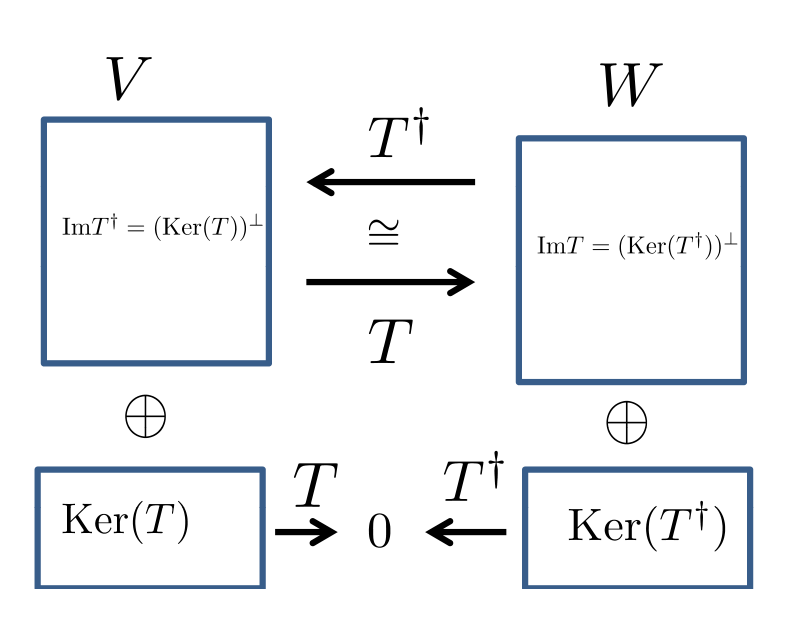
\includegraphics[width=0.72\textwidth]{figures/fig33.png}
  \caption{内积空间之间算符 $T$ 的定义域与值域的正交分解。（原文 Fig.~33，第 196 页）}
  \label{fig:33}
\end{figure}

若 $V,W$ 是内积空间，而 $T:V\to W$ 是一个（足够好的）线性算符，则 $T$ 限制为
$(\ker T)^\perp$ 与 $(\ker T^\dagger)^\perp$ 之间的一个同构，如 33 所示。把它应用于三维的 de Rham 复形，我们便得到这样一幅图景：

{\small\itshape ［原文标记：把 $*$ 解释为等距同构，以及三维流形的特殊情形：］}
% [原文待办标记，原文 p.196：EXPLAIN * AS ISOMETRY AND SPECIAL CASE OF 3-MANIFOLDS:]

\begin{enumerate}
  \item $d$ 与 $d^\dagger$ 作为超对称算符。
  \item $d^\dagger d$ 在 $\Omega^0$ 上的非零谱就是 $dd^\dagger$ 在 $\Omega^3$ 上的谱。记之为 $(\lambda_n^{(0)})^2$。
  \item 在 $\Omega^1$ 上我们有 $dd^\dagger$，其谱为 $(\lambda_n^{(0)})^2$；我们把 $*d$ 对角化，
    本征值为 $\mu_n^{(1)}$，于是 $d^\dagger d$ 的谱为 $(\mu_n^{(1)})^2$。
  \item 在 $\Omega^2$ 上我们有 $dd^\dagger$，其谱为 $(\mu_n^{(1)})^2$；而 $d^\dagger d$ 的谱为 $(\lambda_n^{(0)})^2$。
\end{enumerate}

\begin{figure}[htbp]
  \centering
  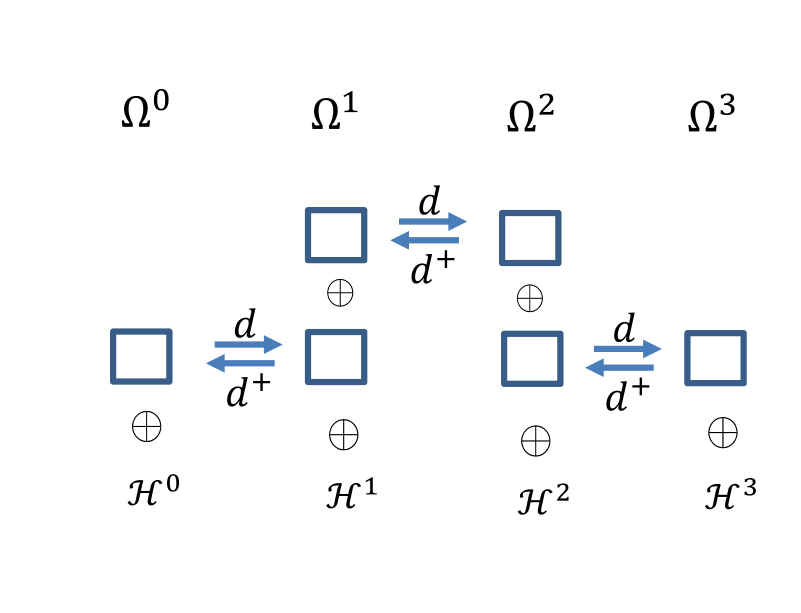
\includegraphics[width=0.80\textwidth]{figures/fig34.png}
  \caption{Riemann 三维流形上 de Rham 复形的 Hodge 分解图示。水平箭头是 Hilbert 空间之间的同构。
    Hodge $*$ 算符是一个等距，它把整幅图关于中心的竖直线翻转过来。这导致解析挠率的有效简化。
    （原文 Fig.~34，第 197 页）}
  \label{fig:34}
\end{figure}

{\small\itshape ［原文标记：图示 Hodge 分解——核对群论笔记。］}
% [原文待办标记，原文 p.197：FIGURE ILLUSTRATING THE HODGE DECOMPOSITION – check Group Theory notes]

\subsection{解析挠率} % 原文: F.2 Analytic Torsion

解析挠率基于如下积分
\begin{equation}
  \tau = \int_0^\infty\frac{dt}{t}\operatorname{Tr}F(-1)^F e^{-tH}
  \tag{F.10}
  \label{eq:F.10}
\end{equation}
其中迹是在 de Rham 复形 $\Omega^*(M)$ 上取的。

基本想法是：若 $\lambda$ 与 $\lambda'$ 有正实部，则
\begin{equation}
  \int_0^\infty\frac{dt}{t}\left(e^{-\lambda t} - e^{-\lambda' t}\right)
  = \log\frac{\lambda'}{\lambda}
  \tag{F.11}
  \label{eq:F.11}
\end{equation}
因此，对两个不同的度规，(F.10) 的两个表达式之差，就是下述量在这两组度规下的差：
\begin{equation}
  \sum_k(-1)^k k\log\operatorname{Det}'(\Delta_k)
  \tag{F.12}
  \label{eq:F.12}
\end{equation}
另一方面，(F.10) 本身是有意义的。我们下面将说明，它与度规无关，因而定义一个拓扑不变量。

这个定义\emph{先验地}依赖于一个度规。取一族度规 $g(s)$ 并对 $s$ 求导：
\begin{equation}
  \dot\tau = -\int_0^\infty dt\,\operatorname{Tr}F(-1)^F\dot H e^{-tH}
  \tag{F.13}
  \label{eq:F.13}
\end{equation}
\begin{equation}
\begin{aligned}
  \dot H &= -(-1)^{nF}\left(\dot{*}d*d + *d\dot{*}d + (-1)^n d\dot{*}d* + (-1)^n d*d\dot{*}\right)\\
  &= -(-1)^{nF}\left(u\delta d - \delta u d + (-1)^n du\delta - (-1)^n d\delta u\right)
\end{aligned}
\tag{F.14}
\label{eq:F.14}
\end{equation}

现在试着把 $-\operatorname{Tr}F(-1)^F\dot H e^{-tH}$ 写成
$\operatorname{Tr}F(-1)^{(n+1)F}ue^{-tH}(\cdots)$ 的形式，必要时循环移动 $d$ 与 $\delta$。注意 $[d,H] = 0$ 且 $[\delta,H] = 0$。

同时我们需要

对 $n = 0\ (2)$：
\begin{equation}
  [F(-1)^F, d] = d(-1)^{F+1}(2F+1)
  \tag{F.15}
  \label{eq:F.15}
\end{equation}
因为 $\left((f+1)(-1)^{f+1} - f(-1)^f\right) = (-1)^{f+1}(2f+1)$。
\begin{equation}
  [F(-1)^F, \delta] = \delta(-1)^{F+1}(2F-1)
  \tag{F.16}
  \label{eq:F.16}
\end{equation}
因为 $\left((f-1)(-1)^{f-1} - f(-1)^f\right) = (-1)^{f-1}(2f-1)$。

对 $n = 1\ (2)$：
\begin{equation}
  [F, d] = d
  \tag{F.17}
  \label{eq:F.17}
\end{equation}
\begin{equation}
  [F, \delta] = -\delta
  \tag{F.18}
  \label{eq:F.18}
\end{equation}

先取 $n = 0\ (2)$。于是我们有
\begin{equation}
\begin{aligned}
  -\operatorname{Tr}F(-1)^F\dot H e^{-tH}
  &= \operatorname{Tr}F(-1)^F\left(u\delta d - \delta u d + du\delta - d\delta u\right)e^{-tH}\\
  &= -\frac{d}{dt}\left(\operatorname{Tr}(-1)^F u e^{-tH}\right)
\end{aligned}
\tag{F.19}
\label{eq:F.19}
\end{equation}

% [Tutor Note: (F.14) 到 (F.19) 之间省略了「循环移动」的全部步骤：把 (F.14) 的
% 四项各自用 $[d,H]=[\delta,H]=0$（故 $e^{-tH}$ 可自由穿过 $d,\delta$）、
% $d^2=\delta^2=0$ 以及 $\operatorname{Tr}$ 的循环性搬到 $u$ 的同侧，再用
% (F.15)--(F.18) 的交换子把 $F$ 的因子提出。搬动过程中穿过 $(-1)^F$ 会带来
% (F.15)--(F.18) 那样的符号；若只把 $d,\delta$ 当普通矩阵交换，会丢掉
% $(-1)^{F+1}(2F\pm1)$ 中的 $2F$ 项，(F.19) 的第二行就不再是全导数。]

现在我们可以分部积分。在 $t = 0$ 附近我们有 $\operatorname{Tr}(-1)^F u e^{-\epsilon H}$。
它是 $\operatorname{Tr}(-1)^F u$ 的一个正则化版本。后者形式上是零，因为 $*$ 同时是 de Rham 复形偶子复形与奇子复形的等距，所以我们是在取一个反对称算符的迹。

现在考虑 $n = 1\ (2)$。
\begin{equation}
\begin{aligned}
  -\operatorname{Tr}F(-1)^F\dot H e^{-tH}
  &= \operatorname{Tr}F\left(u\delta d - \delta u d - du\delta + d\delta u\right)e^{-tH}\\
  &= -\frac{d}{dt}\left(\operatorname{Tr}(-1)^F u e^{-tH}\right)
\end{aligned}
\tag{F.20}
\label{eq:F.20}
\end{equation}

我们再分部积分一次。为处理下限，注意 $u$ 与 $(-1)^F$ 对易，并且也把
$\Omega^k\to\Omega^k$。若它可以对角化，则它在 $\Omega^k$ 与 $\Omega^{n-k}$ 上有相同的本征值，
于是 $(-1)^F u$ 的本征值相反，从而至少在形式上 $\operatorname{Tr}(-1)^F u = 0$。

对三维流形的情形
\begin{equation}
\begin{aligned}
  \tau &= -\log\det\Delta^{(1)} + 2\log\det\Delta^{(2)} - 3\log\det\Delta^{(3)}\\
  &= \log\prod_n(\mu_n^{(1)})^2 - 2\log\prod_n(\lambda_n^{(0)})^2
\end{aligned}
\tag{F.21}
\label{eq:F.21}
\end{equation}

\section{流形上的定向、Spin、Spin$^c$、$Pin^{\pm}$ 与 Pin$^c$ 结构} % 原文: G. Orientation, Spin, Spin^c, Pin^±, And Pin^c Structures On Manifolds

\begin{keytakeaways}
  \item 定义：沿同态 $\phi:G_1\to G_2$ 把主 $G_2$ 丛 $P_2$ 约化到 $G_1$，就是给一个主 $G_1$ 丛 $P_1$
    连同同构 $P_1\times_{G_1}G_2\cong P_2$，即交换图 (G.1)；等价的说法是：过渡函数取在 $G_1$ 中，
    并逐点经 $\phi$ 映到 $G_2$。
  \item 三类几何例子：子群包含（$P/H$ 的截面给出子丛，$H=\{1\}$ 时即「整体截面平凡化丛」）、
    $O(n)\subset GL(n,\mathbb{R})$（Riemann 度量把标架丛约化为正交标架丛）、
    $SO(n)\subset O(n)$（截面即定向）。
  \item 覆盖映射的情形：$\phi:\tilde G\to G$ 满射、核为 $K$ 时，「约化」实际是提升——给的是覆盖 $P$
    的主 $\tilde G$ 丛 $\tilde P$，满足 $\tilde P/K\cong P$（图 (G.2)）；作者本人指出「约化」一词在此有误导。
  \item 本节标题所列的 Spin、Spin$^c$、$Pin^{\pm}$、Pin$^c$ 结构，都将作为上述框架中不同 $\phi$ 的特例出现。
\end{keytakeaways}

\subsection{结构群约化：一般讨论} % 原文: G.1 Reduction Of Structure Group: General Discussion

给定两个紧 Lie 群 $G_1,G_2$ 以及一个同态 $\phi:G_1\to G_2$，我们可以定义一个函子 $F_\phi$，从 $M$ 上的主 $G_1$ 丛到 $M$ 上的主 $G_2$ 丛，其作法是：把主 $G_1$ 丛 $G_1\to P\to M$ 送到 $(P\times_{G_1}G_2)\to M$。回忆 $(P\times_{G_1}G_2)$ 是
对 $(p,g)\in P\times G_2$ 在等价关系 $(ph,g) = (p,\phi(h)g)$（$h\in G_1$）下的等价类之集，且它显然带有一个自由的右 $G_2$ 作用。

\begin{definition}[原文未编号]
  若 $G_2\to P_2\to M$ 是一个主 $G_2$ 丛，则\emph{沿 $\phi:G_1\to G_2$ 到 $G_1$ 的一个约化}
  是一个主 $G_1$ 丛 $G_1\to P_1\to M$ 连同一个同构 $\psi$，使得我们有如下交换图：
\begin{equation}
  \begin{array}{ccc}
    (P_1\times_{G_1}G_2) & \xrightarrow{\ \psi\ } & P_2\\[4pt]
    \searrow & & \downarrow\\[4pt]
    & M &
  \end{array}
  \tag{G.1}
  \label{eq:G.1}
\end{equation}
\end{definition}

把定义展开一遍，就可以用贴片重叠 $\mathcal{U}_{\alpha\beta}$ 上的过渡函数给出描述。若
$h_{\alpha\beta}:\mathcal{U}_{\alpha\beta}\to G_1$ 是 $P_1$ 的过渡函数，则作为主 $G_2$ 丛，$P_2$
与一个过渡函数为 $\phi(h_{\alpha\beta}):\mathcal{U}_{\alpha\beta}\to G_2$ 的丛同构。

\paragraph{例子}
\begin{enumerate}
  \item 若 $\phi:H\to G$ 是一个子群的包含，则给定 $G$ 丛 $P\to M$，$H$ 自由作用，
    于是我们可以考虑 $G/H\to P/H\to M$，即一个齐性空间丛。在此情形，丛 $P/H$ 的一个截面
    给出 $P$ 到 $H$ 丛的一个约化，而后者事实上是一个子丛。作为特例，取 $H = \{1\}$。
    这正是众所周知的事实：主 $G$ 丛的一个整体截面使该丛平凡化。
  \item 取 $H = O(n)$、$G = GL(n,\mathbb{R})$。一个度量把标架丛约化为正交标架丛
    $\mathcal{B}_O(M)$。显然，正交标架丛是标架丛的子丛。
  \item 设 $M$ 是一个 Riemann 流形，$H = SO(n)$、$G = O(n)$，而 $\phi$ 是包含。
    则 $\mathcal{B}_O(M)/H$ 是定向二重覆盖。若 $M$ \emph{可定向}，则定向丛有截面。
    事实上，若 $M$ 连通，$\mathcal{B}_O(M)$ 有两个连通分支，因而有两个截面。
    选取一个截面给出该丛到 $SO(n)$ 定向标架丛的约化。截面的选取就是 $M$ 定向的选取。
  \item 现在设 $\phi$ 是一个覆盖映射，即 $\phi:\tilde G\to G$ 是\emph{满射}、核为 $K$。
    于是把主 $G$ 丛 $P$「约化」为主 $\tilde G$ 丛 $\tilde P$，就是一个同构
\begin{equation}
  \begin{array}{ccc}
    \tilde P/K & \xrightarrow{\ \psi\ } & P\\[4pt]
    \searrow & & \downarrow\\[4pt]
    & M &
  \end{array}
  \tag{G.2}
  \label{eq:G.2}
\end{equation}
\end{enumerate}

% [Tutor Note: 术语取舍。reduction of structure group 译为「结构群约化」，这是中文
% 文献的通行译法；但如第 4 例所示，覆盖映射情形下「约化」得到的 $\tilde P$ 其实是
% $P$ 的提升（覆盖），而不是子丛，作者因此说这个词「有误导性」。另一种译法是
% 「结构群的提升」；本译本统一用「约化」以与原文一致，遇到第 4 例时按此理解即可。]

注意一般定义中的「约化」一词有误导性，因为 $\tilde P$ 实际上是 $P$ 的一个覆盖。换个说法，主 $G$
% [跨页衔接：本句在原文 p.199 底部被截断，后半句「丛 $P$ 到 $\tilde G$ 的约化，等同于
%  一个覆盖 $P$ 的主 $\tilde G$ 丛 $\tilde P$」由下一片段 c25 的开头接续。]

% =====================================================================
%  c25 —— 原文印刷页 200--210（PDF 第 201--211 页）
%  含：附录 G 的 G.2（自旋与 Pin 结构的阻碍）、G.3（四维流形上的 Spin^c 结构）、
%      G.4（'t Hooft 磁通）；附录 H（联络、平行移动与和乐）之开头，至 (H.35) 止
%  编号公式：G.3--G.23（其中 (G.9) 是原稿的一条空白编号行）与 H.1--H.35，共 56 条
%  插图：Fig. 35（印刷第 207 页）、Fig. 36（印刷第 209 页）
%  全部公式均逐条对照 150 dpi 页面图像转写（文本层仅供读散文）
% =====================================================================

% 说明：本片段从 G.1 的编号列表第 4 条中间切入（G.1、G.2 在上一片段 c24 中），
%  故开头是一句残句，此处不补 \section{G} 标题。

……丛 $P$ 到 $\widetilde{G}$ 的（结构群）约化，等同于一个覆盖 $P$ 的主 $\widetilde{G}$ 丛 $\widetilde{P}$：

\begin{equation}
  \widetilde{P} \to P \to M
  \tag{G.3}
  \label{eq:G.3}
\end{equation}

使得每一点 $m\in M$ 上方的纤维「看起来像」覆盖

\begin{equation}
  1 \to K \to \widetilde{G} \to G \to 1
  \tag{G.4}
  \label{eq:G.4}
\end{equation}

\begin{enumerate}[start=5]
  \item 定向流形上\emph{自旋结构}（spin structure）的选取，是前述注记 \eqref{eq:G.2} 在
    $\phi:\mathrm{Spin}(n)\to SO(n)$ 这一情形下的特例。为了对自旋结构分类，我们先按
    $z\in H^1(\mathcal{B}_{SO}(M);\mathbb{Z}_2)$ 对 $\mathcal{B}_{SO}(M)$ 上的主 $\mathbb{Z}_2$ 丛分类。
    自旋结构就是那些限制到纤维上给出二重覆盖 $\mathrm{Spin}(n)\to SO(n)$ 的丛。二重覆盖
    $\mathrm{Spin}(n)\to SO(n)$ 对应于 $z_s\in H^1(SO(n);\mathbb{Z}_2)\cong\mathbb{Z}_2$。
    因此，自旋结构就是 $\mathcal{B}_{SO}(M)$ 的那些二重覆盖：它们限制到纤维
    $\mathcal{B}_{SO}(M)\to M$ 上给出类 $z_s$。注意两个自旋结构之差 $z_1-z_2$ 于是在纤维上是平凡的，
    从而拉回自 $H^1(M;\mathbb{Z}_2)$ 中的某个类。于是 $M$ 上的自旋结构构成
    $H^1(M;\mathbb{Z}_2)$ 的一个 torsor（主齐性空间）。

  \item 用同样的办法可以处理其它结构。对流形 $M$，基于把上述概念施用于同态
    \begin{equation}
      \phi : \mathrm{Pin}^c \to O(n)
      \tag{G.5}
      \label{eq:G.5}
    \end{equation}
    \begin{equation}
      \phi : \mathrm{Spin}^c \to O(n)
      \tag{G.6}
      \label{eq:G.6}
    \end{equation}
    \begin{equation}
      \phi : \mathrm{Pin}^{\pm} \to O(n)
      \tag{G.7}
      \label{eq:G.7}
    \end{equation}
    \begin{equation}
      \phi : \mathrm{Spin} \to O(n)
      \tag{G.8}
      \label{eq:G.8}
    \end{equation}
    \begin{equation}
      \tag{G.9}
      \label{eq:G.9}
    \end{equation}
    我们便可以谈论 $\mathrm{Pin}^c$、$\mathrm{Spin}^c$、$\mathrm{Pin}^{\pm}$、$\mathrm{Spin}$ 结构。
    注意这些同态一般既不是单射也不是满射。对于定向流形上的 BLOTZ 结构，我们把类似的同态施用于
    定向标架丛，即取值到 $SO(n)$。

    % 说明：原文 (G.9) 只有编号、没有公式体，是作者删掉一条式子后留下的空白编号行；
    %  此处照原样保留空公式，编号 G.10 及以后仍与页面图像一致。另：原文的 "BLOTZ structure"
    %  是一个未定义的占位词（字母串），疑为作者留给自己的结构名占位（按上下文应是某种
    %  twisted Pin/Spin 结构），不要擅自改写成 "Bloch"。
\end{enumerate}

\subsection{自旋与 Pin 结构的阻碍} % 原文: G.2 Obstructions To Spin And Pin Structures

把上面略嫌抽象的表述翻译成流形 $X$ 的切丛的转移函数的语言，是值得做的。设
$\{\mathcal{U}_{\alpha\beta}\}$ 是 $X$ 的坐标图册。利用度规我们可以取正交标架，若
$\dim_{\mathbb{R}}X=n$，它们有转移函数

\begin{equation}
  g_{\alpha\beta} : \mathcal{U}_{\alpha\beta} \to O(n)
  \tag{G.10}
  \label{eq:G.10}
\end{equation}

若我们能用一个上链把它们修改为

\begin{equation}
  \tilde{g}_{\alpha\beta} = h_\alpha g_{\alpha\beta} h_\beta^{-1}
  \tag{G.11}
  \label{eq:G.11}
\end{equation}

其中 $h_\alpha:\mathcal{U}_\alpha\to O(n)$，使得 $\tilde{g}_{\alpha\beta}:\mathcal{U}_{\alpha\beta}\to SO(n)$，
则流形是可定向的。可定向性的唯一阻碍由 Cech 2-上链
$\det g_{\alpha\beta}:\mathcal{U}_{\alpha\beta}\to\mathbb{Z}_2$ 提供，它定义上同调类
$w_1(X)\in H^1(X;\mathbb{Z}_2)$。注意若 $X$ 单连通，则 $H^1(X;\mathbb{Z}_2)=0$，因而它必定可定向。

% [Tutor Note: 指标个数与上链次数的错位是这一段最易读错的地方。Cech 理论中，以
%  $p+1$ 个开集为下标的族是一个 $p$-上链，所以以 $\alpha\beta$ 两个下标标注的
%  $\det g_{\alpha\beta}$ 是 1-上链、给出 $H^1$ 中的 $w_1$；而下面 (G.12) 中以
%  $\alpha\beta\gamma$ 三个下标标注的 $\xi_{\alpha\beta\gamma}$ 虽是「3-上链」（three indices），
%  它对应的却是 $H^2$ 中的 $w_2$。原文把后者称为 "Cech 3-cocycle"，指的是三个下标，
%  不是三次上同调。]

当 $X$ 可定向时，我们可以取 $g_{\alpha\beta}:\mathcal{U}_{\alpha\beta}\to SO(n)$。若选取\emph{良覆盖}
（good cover），即所有交 $\mathcal{U}_{\alpha\beta\cdots}$ 都是可缩的，则在每个重叠
$\mathcal{U}_{\alpha\beta}$ 上我们可以选取提升
$\tilde{g}_{\alpha\beta}:\mathcal{U}_{\alpha\beta}\to\mathrm{Spin}(n)$。唯一的问题是这样提升之后
上链条件可能失效。由于我们已取定提升，而覆盖 $\mathrm{Spin}(n)\to SO(n)$ 的核恰是群
$\{\pm1\}$，我们可以确知在 $\mathcal{U}_{\alpha\beta\gamma}$ 上

\begin{equation}
  \tilde{g}_{\alpha\beta}(x)\tilde{g}_{\beta\gamma}(x)\tilde{g}_{\gamma\alpha}(x)
  := \xi_{\alpha\beta\gamma}\in\{\pm1\}\subset \mathrm{Spin}(n)
  \qquad \forall x\in\mathcal{U}_{\alpha\beta\gamma}
  \tag{G.12}
  \label{eq:G.12}
\end{equation}

符号 $\xi_{\alpha\beta\gamma}$ 定义一个 Cech 3-上链，它定义 $H^2(X;\mathbb{Z}_2)$ 中的一个上同调类。
这是 $w_2$ 的一个（非常具体的）定义。注意：把提升 $g_{\alpha\beta}$ 乘上一个上链而作任意修改，
或者取不同的提升 $\tilde{g}_{\alpha\beta}$，都只把 $\{\xi_{\alpha\beta\gamma}\}$ 改变一个上边界。
几乎按定义，这就是自旋结构存在的唯一阻碍。

\begin{enumerate}
  \item 最简单的非平凡例子是圆上的自旋结构。圆是一维的，故取 $n=1$。此时 $SO(1)$ 是平凡群，
    而 $\mathrm{Spin}(1)\cong\mathbb{Z}_2$。于是圆上的自旋结构字面上就是圆的二重覆盖。这样的覆盖有两个：
    平凡的一个与非平凡的一个。在物理中它们分别称为 \emph{Neveu-Schwarz} 与 \emph{Ramond} 自旋结构。
    注意平凡的二重覆盖可以延拓为圆盘的二重覆盖，但圆的非平凡二重覆盖不能延拓到圆盘上。

    令人有些困惑的是：相对于某个自然的平凡化，Neveu-Schwarz 自旋结构中的旋量应看成圆上的
    反周期函数，而 Ramond 自旋结构中的旋量应看成周期函数。看清这一点的一个办法是直接考虑
    圆盘上的欧氏度规，取正交标架 $e_1=dr$、$e_2=rd\theta$。此时 $\omega_{12}=-d\theta$ 就是自旋联络。
    现在考虑协变旋量方程

    \begin{equation}
      D_\mu\psi = \partial_\mu\psi + \frac{1}{4}\omega_\mu^{ab}\gamma^{ab}\psi = 0
      \tag{G.13}
      \label{eq:G.13}
    \end{equation}

    而在圆盘上的自旋丛中我们可以取常旋量表示

    \begin{equation}
      \gamma^1 = i\sigma^1 \qquad \gamma^2 = i\sigma^2
      \tag{G.14}
      \label{eq:G.14}
    \end{equation}

    于是普遍的协变旋量为

    \begin{equation}
      \psi = \left( c_1 e^{-i\theta/2}\begin{pmatrix} 1 \\ 0 \end{pmatrix}
        + c_2 e^{i\theta/2}\begin{pmatrix} 0 \\ 1 \end{pmatrix} \right)
      \tag{G.15}
      \label{eq:G.15}
    \end{equation}

    % [Tutor Note: (G.13) 的因子 $1/4$ 与 $e^{\mp i\theta/2}$ 的相位要一起核对：
    %  $\gamma^{ab}=\frac12[\gamma^a,\gamma^b]$，$\omega_{12}=-d\theta$，故
    %  $\frac14\omega_\mu{}^{12}\gamma_{12}$ 中的 $\frac14$ 实际抵消了 $\gamma_{12}$ 定义里的 $\frac12$，
    %  最后给出 $\mp\frac{i}{2}\dot\theta$，积分后正是 $\mp i\theta/2$。若漏掉 $\frac12$
    %  就会得到整数相位的「旋量」，从而把 Neveu-Schwarz 与 Ramond 两种结构搞混。]

    {\small\itshape ［原文标记：这一点仍然令人困惑，因为这些波函数并不延拓到圆盘上；上面的旋量函数是相对于
    $K^{1/2}$ 的一个不延拓到圆盘上的平凡化而言的。仍需更完整地解释。Witten 关于超弦微扰论的工作中
    也许有些好的评论。］}

    % [原文待办标记，原文 p.201--p.202：作者用一行星号围出的大段自注，跨页收尾；
    %  星号内文字保留原意译出。]

    {\small\itshape ［原文标记：下面两个例子都假定 $X$ 是四维的］}

    % [原文待办标记，原文 p.202 右侧页边 \ensuremath{\clubsuit}…\ensuremath{\clubsuit} 注]

  \item 一个例子：$\mathcal{B}SO(2)=\mathcal{B}U(1)=\mathbb{C}P^\infty$。$w_2$ 是 $c_1$ 的模二约化，
    而 $c_1$ 是与 2-胞腔对偶的上链。所以请解释为什么 $c_1\bmod 2$ 是自旋结构的阻碍。在
    $\mathbb{C}P^2$ 上 $c_1=3x$。复化切丛允许把
    $SO(4)=SU(2)\times SU(2)/\mathbb{Z}_2$ 的结构群约化到
    $U(2)=SU(2)\times U(1)/\mathbb{Z}_2$。限制到 $\mathbb{C}P^1\subset\mathbb{C}P^2$ 上，切丛分裂为
    $\mathcal{O}(2)\oplus\mathcal{O}(1)$，其中 $\mathcal{O}(2)$ 是 $\mathbb{C}P^1$ 的切丛，
    而 $\mathcal{O}(1)$ 是法丛。结构群进一步约化到 $U(1)\times U(1)$。显然，与法丛
    $\mathcal{O}(1)$ 相伴的主 $U(1)$ 丛不容许一个二重覆盖，使其在 $U(1)$ 上限制为 $U(1)$ 的二重覆盖。

  \item 对 $\mathrm{Spin}^c$ 结构的阻碍是 $W_3$，即 $w_2$ 在 Bockstein 映射下的像。因此当
    $w_2(X)\in H^2(X;\mathbb{Z}_2)$ 具有整提升时它为零。利用对一切 $\sigma\in H_2(X;\mathbb{Z})$ 有

    \begin{equation}
      \int_\sigma w_2(X) = \sigma\cdot\sigma \ \ \mathrm{mod}\ 2
      \tag{G.16}
      \label{eq:G.16}
    \end{equation}

    其中 $\sigma\cdot\sigma$ 是定向整相交数，便可以证明这样的整提升确实存在。细节见 [?]。
    在不可定向的情形下类似的命题不成立：$\mathbb{R}P^2\times\mathbb{R}P^2$ 不容许
    $\mathrm{Pin}^c$ 结构。此外，还存在非 $\mathrm{Spin}^c$ 的定向五维流形。一个简单的例子是
    对称 $SU(3)$ 矩阵构成的空间，它微分同胚于 $SU(3)/SO(3)$。解释见 [?]。

    % [Tutor Note: (G.16) 左边是对 2-维闭链 $\sigma\in H_2(X;\mathbb{Z})$ 积分，右边是相交数，
    %  两者都是整（或模 2）量，但只有在 $X$ 定向且四维时 $\sigma\cdot\sigma$ 才有定义——
    %  这正是作者在旁边标注「下面两个例子假定 $X$ 四维」的原因。$W_3=\beta(w_2)$（Bockstein），
    %  不是另一个 Stiefel-Whitney 类，别把 $W_3$ 与 $w_3$ 混淆：$w_3$ 属于 $H^3$，而
    %  $W_3\in H^3(X;\mathbb{Z})$ 是 $w_2$ 的整 Bockstein 提升，其消失才是 $\mathrm{Spin}^c$ 存在的判据。]

    {\small\itshape ［原文标记：另见 Gompf、Stipsicz《4-Manifolds and Kirby Calculus》中的证明］}

    % [原文待办标记，原文 p.202 右侧页边 \ensuremath{\clubsuit}Also look up proof in Gompf, Stipszic … \ensuremath{\clubsuit}]

    {\small\itshape ［原文标记：给出证明。］}

    % [原文待办标记，原文 p.202 右侧页边 \ensuremath{\clubsuit}Give proof. \ensuremath{\clubsuit}，紧接在「五维流形」一句旁]
\end{enumerate}

\subsection{四维流形上的 $\mathrm{Spin}^c$ 结构} % 原文: G.3 Spin^c Structures On Four-Manifolds

群 $\mathrm{Spin}^c(4)$ 定义为

\begin{equation}
  \mathrm{Spin}^c(4) := \left(\mathrm{Spin}(4)\times U(1)\right)/\mathbb{Z}_2
  = \left(SU(2)\times SU(2)\times U(1)\right)/\mathbb{Z}_2
  \tag{G.17}
  \label{eq:G.17}
\end{equation}

其中我们除以按 $(-1,-1,-1)$ 嵌入的群 $\mathbb{Z}_2$。$X$ 的定向正交标架丛 $OrFr(X)$ 是主 $SO(4)$ 丛，
而自旋 $c$ 结构——按定义——是结构群到由显然同态 $\mathrm{Spin}^c(4)\to SO(4)$ 所定义的主
$\mathrm{Spin}^c(4)$ 丛的约化。把定义写开就意味着：自旋 $c$ 结构由一个主 $\mathrm{Spin}^c(4)$ 丛
$\mathfrak{P}$ 连同投影 $\mathfrak{P}\to OrFr(X)$ 给出，该投影沿着纤维看起来像正合列

\begin{equation}
  1 \to U(1) \to \mathrm{Spin}^c(4) \to SO(4) \to 1
  \tag{G.18}
  \label{eq:G.18}
\end{equation}

当 $w_2(X)$ 具有整提升时，自旋 $c$ 结构存在。如上所述，对每个紧定向四维流形这确实成立。

由 $[(v_L,v_R,\zeta)]\mapsto(\zeta v_L,\zeta v_R)$ 给出的群同态
$\mathrm{Spin}^c(4)\to U(2)\times U(2)$ 定义一个同构

\begin{equation}
  \mathrm{Spin}^c(4) \cong \left\{ (u_L,u_R)\mid \det u_L = \det u_R \right\}
  \subset U(2)\times U(2)
  \tag{G.19}
  \label{eq:G.19}
\end{equation}

后一表述使下面这件事变得显然：$\mathrm{Spin}^c(4)$ 有两个不等价的秩 2 表示 $W^{\pm}$，
它们就由两个 $U(2)$ 因子的基本表示定义。给定一个自旋 $c$ 结构，于是有两个相伴的复秩二丛
$W^{\pm}\to X$，并且在上面{\small\itshape ［原文标记：section ??（章节交叉引用待补，原稿占位符）］}
的讨论中我们可以认定

% [原文标记：原文此处写 "in the discussion of section ?? above"，章节号是作者留的占位符，
%  至今未填；对照 p.203 的上下文应是指前面讨论 Dirac 旋量丛 $S^\pm$ 与线丛 $L$ 的那一节。]

\begin{equation}
  W^{\pm} = S^{\pm}\otimes L
  \tag{G.20}
  \label{eq:G.20}
\end{equation}

反之，这样一对丛 $W^{\pm}$ 定义一个自旋 $c$ 结构。因此自旋 $c$ 结构的空间是线丛群的一个 torsor：
因为给定线丛 $\mathcal{L}$，我们总可以取

\begin{equation}
  W^{\pm} \to W^{\pm}\otimes\mathcal{L}
  \tag{G.21}
  \label{eq:G.21}
\end{equation}

使得

\begin{equation}
  c_1(\det W^{\pm}) \to c_1(\det W^{\pm}) + 2c_1(\mathcal{L})
  \tag{G.22}
  \label{eq:G.22}
\end{equation}

注意：给定 $X$ 上的近复结构，就有一个典范的自旋 $c$ 结构

\begin{equation}
  W^{+} = \Omega^{0,0}(X)\oplus\Omega^{0,2}(X)
  \qquad\qquad
  W^{-} = \Omega^{0,1}(X)
  \tag{G.23}
  \label{eq:G.23}
\end{equation}

% [Tutor Note: (G.22) 中的因子 2 不能漏。(G.20) 说 $W^{\pm}=S^{\pm}\otimes L$ 且
%  $\det S^{\pm}=1$（$S^{\pm}$ 是 $SU(2)$ 的秩 2 丛），故 $\det W^{\pm}=L^{2}$，于是
%  $\det W^{\pm}$ 的行列式线丛在 $L\to L\otimes\mathcal{L}$ 下按 $L^2\to L^2\otimes\mathcal{L}^2$
%  变换，正是 (G.22)。这也解释了自旋 $c$ 结构的 torsor 结构为何是「线丛群」而不是
%  「$H^2$ 的元素」：$L$ 与 $L\otimes\mathcal{L}$ 给出不同但同伦等价的 $W^{\pm}$。]

\subsection{'t Hooft 磁通} % 原文: G.4 ’t Hooft Flux

在讲义的好几处，我们用到主 $SO(3)$ 丛 $P$ 的第二 Stiefel-Whitney 类 $w_2(P)$。一般地，
流形 $M$ 上的 $SO(n)$ 丛 $P$ 有一个特征类 $w_2(P)\in H^2(M;\mathbb{Z}_2)$。定义它的一种办法
沿用上面关于自旋结构的讨论：选取 $M$ 的良覆盖 $\{\mathcal{U}_\alpha\}$ 以及 $P$ 在该覆盖上的平凡化。
在重叠 $\mathcal{U}_{\alpha\beta}$ 上选取提升
$\tilde{g}_{\alpha\beta}:\mathcal{U}_{\alpha\beta}\to\mathrm{Spin}(n)$，并度量上链条件在
$\mathcal{U}_{\alpha\beta\gamma}$ 上失效的程度，从而定义 $H^2(M;\mathbb{Z}_2)$ 中的一个类。
若 $w_2(P)$ 非零，则 $P$ 的结构群不能从 $SO(n)$ 约化到 $\mathrm{Spin}(n)$。

不能提升为 $\mathrm{Spin}(n)$ 丛的 $SO(n)$ 丛的一个简单例子如下：取 $M$ 为二维紧曲面。
选一点 $p\in M$ 以及 $p$ 周围的小圆盘。用绕圆盘边界的转移函数在 $SO(n)$ 中定义一条非平凡闭路，
以此定义一个 $SO(n)$ 丛。

\section{联络、平行移动与和乐} % 原文: H. Connections, Parallel Transport, And Holonomy

\begin{keytakeaways}
  \item 联络的路径提升定义：沿路径 $x(t)$ 解一阶线性 ODE
    $\frac{d}{dt}\vec{v}=A(x(t))\dot{x}\vec{v}$，其解算子就是路径排序指数
    $\mathbb{U}(\wp_t)=\mathrm{Pexp}\int_0^t A(x(t_1))\dot{x}_1dt_1$，它只依赖 $A$ 沿该路径的取值
    （而与重参数化 $t\to f(t)$、$f'>0$ 无关）。
  \item 乘法律的方向：路径提升 $\mathbb{P}$ 对复合协变，$\mathbb{P}(\wp_1\star\wp_2)=\mathbb{P}(\wp_1)\star\mathbb{P}(\wp_2)$；
    而矩阵解 $\mathbb{U}$ 对复合\emph{反变}，$\mathbb{U}(\wp_1\star\wp_2)=\mathbb{U}(\wp_2)\mathbb{U}(\wp_1)$。
    这是路径排序指数最常被记反的约定。
  \item 单值性即曲率：小环路 $\mathbb{U}(\wp)=1+\alpha F_{z\bar z}(z_0,\bar z_0)+O(\epsilon^3)$，
    其中 $\alpha$ 是环路所围面积的两倍，一般的实坐标版本是
    $\mathbb{U}(\wp)=1-\epsilon_1\epsilon_2F_{\mu\nu}(\vec{x}_0)+\cdots$。
  \item 平坦联络（$F=0$）的单值性只依赖路径的同伦类：把同伦映射的 $I^2$ 剖分成足够小的方块，
    每块的环路单值性平凡，故整体平凡。
  \item 联络是 1-形式：换坐标时必须用 $\tilde{A}(z)dz=A(x)dx$ 而非 $\tilde{A}(z)=A(x)$ 来定义，
    即 $\tilde{A}(z)=\frac{1}{2\pi i}e^{-2\pi ix}A(x)$；规范变换律为
    $A=g^{-1}\widetilde{A}g+g^{-1}dg$。
\end{keytakeaways}

{\small\itshape ［原文标记：用路径提升性质给出联络的定义］}

% [原文待办标记，原文 p.203：作者以待办口吻写的缺节提示，用星号行围出，星号行跨页至
%  p.204 顶部才收尾；星号行内的 "Our convention for concatenating curves" 与 (H.1)
%  是正文内容，故按普通正文排出。]

我们拼接曲线的约定是：

\begin{equation}
  f_1 \star f_2(t) :=
  \begin{cases}
    f_1(2t) & 0\le t\le \tfrac12 \\[2pt]
    f_2(2t-1) & \tfrac12\le t\le 1
  \end{cases}
  \tag{H.1}
  \label{eq:H.1}
\end{equation}

% [原文标记：星号行在同一待办块内跨页，p.204 顶部以一行星号收尾；此后正文接续。]

对于主丛与向量丛，我们可以把该性质用局部微分方程表达出来，从而建立它与局部定义的矩阵值
1-形式之间的联系。

\textbf{例 1}\quad 最初步的例子取 $B=\mathbb{R}$、$E=\mathbb{R}\times\mathbb{C}^n$，
而 $p:E\to B$ 就是到第一个因子的投影，即 $p(x,\vec{v})=x$。现在给定 $B$ 中由 $x(t)$、
$0\le t\le 1$ 给出的路径 $\wp$，我们可以通过选取一个取值在 $n\times n$ 复矩阵中的 $x$ 的函数
来定义路径提升规则，即一个联络。把它记作 $A(x)$。于是路径提升规则是：

\begin{enumerate}
  \item 若 $\wp$ 是一条路径 $\wp: x_0\rightsquigarrow x_1$，则在起点上方的纤维中选取一个元素
    $e_0=(x_0,\vec{v}_0)$。

  \item 然后求解常微分方程，边界条件由初始点的提升 $e_0$ 给出：
    \begin{equation}
      \frac{d}{dt}\vec{v}(t) = A(x(t))\frac{dx}{dt}\vec{v}(t)
      \qquad \vec{v}(0)=\vec{v}_0.
      \tag{H.2}
      \label{eq:H.2}
    \end{equation}
\end{enumerate}

于是提升路径的规则（由 $A(x)$ 的选取决定）是

\begin{equation}
  \mathbb{P}(\wp)(t) := (x(t),\vec{v}(t))
  \tag{H.3}
  \label{eq:H.3}
\end{equation}

见{\small\itshape ［原文标记：Figure ??（图号未定，原文占位符）］}。

% [原文标记：原文此处写 "See Figure ??."，图号是作者留的占位符；按上下文应指例 1 中
%  「沿路径提升向量」的示意图，该图在本稿中始终没有画出。]

这条规则确实与路径的复合相容，理由是方程 \eqref{eq:H.2} 在时间 $t$ 的重参数化 $t\to f(t)$ 下不变，
只要 $f(t)$ 可微且 $f'(t)>0$。利用这一点以及一阶线性 ODE 解的存在唯一性，我们有

\begin{equation}
  \mathbb{P}(\wp_1\star\wp_2) = \mathbb{P}(\wp_1)\star\mathbb{P}(\wp_2)
  \tag{H.4}
  \label{eq:H.4}
\end{equation}

\paragraph{注记}

\begin{enumerate}
  \item 这里我们假定 $\wp$ 是分段可微路径，即 $x(t)$ 是连续函数、在区间上可微（但导数可以在孤立点处不连续）。
  \item 我们假定 $A(x)$ 在路径上非奇异。
  \item 注意由于该微分方程在复共轭下不变，若 $A(x)$ 是实的，则当 $\vec{v}_0$ 为实时解 $\vec{v}(t)$ 也为实。
\end{enumerate}

{\small\itshape ［原文标记：我们真应该把路径排序指数的约定改成
$\mathbb{U}(\wp_1*\wp_2)=\mathbb{U}(\wp_1)\mathbb{U}(\wp_2)$］}

% [原文待办标记，原文 p.204 右侧页边 \ensuremath{\clubsuit}WE SHOULD REALLY CHANGE CONVENTION ON OUR PATH
%  ORDERED EXPONENTIAL SO THAT U(℘_1 ∗ ℘_2) = U(℘_1)U(℘_2). \ensuremath{\clubsuit} —— 正文 (H.8) 给的是反变乘法律，
%  与此处作者想改成的协变约定正好相反，见下面的 Tutor Note。]

% [Tutor Note: (H.4) 与 (H.8) 的方向相反是本节最易错的地方，不是笔误。$\mathbb{P}$ 作用在
%  「点+向量」上，先走 $\wp_1$ 再走 $\wp_2$，故协变；而 $\mathbb{U}$ 是作用在固定初始纤维上的
%  矩阵，$\mathbb{U}(\wp_1)$ 把 $t=0$ 的数据送到 $t=1$，复合时必须先乘后一段的矩阵，
%  故反变。作者自己在 p.204 页边注里说想改用协变约定（那样 (H.13) 的指数就要写成
%  $\mathrm{Pexp}\int A\dot{x}$ 的反序或右作用于行向量），但全书正文一律沿用 (H.8) 的反变约定。]

\paragraph{路径排序指数}

% [原文以斜体下划线标出的无编号小标题 "The path ordered exponential"，非编号标题，
%  故用 \paragraph 复刻。]

事实上，可以写出微分方程 \eqref{eq:H.2} 的一个「显式」解，而这个表示可能很有用。解可以写成如下形式。
定义一个 $n\times n$ 复矩阵：

\begin{equation}
  \begin{aligned}
    \mathbb{U}(\wp_t) := {}& 1 + \int_0^t A(x(t_1))\dot{x}(t_1)dt_1 \\
    &+ \sum_{m=2}^{\infty}\int_0^t dt_1\int_0^{t_1}dt_2\cdots\int_0^{t_{m-1}}dt_m\,
      A(x(t_1))\dot{x}_1\cdots A(x(t_m))\dot{x}_m
  \end{aligned}
  \tag{H.5}
  \label{eq:H.5}
\end{equation}

于是我们有

\begin{equation}
  \vec{v}(t) = \mathbb{U}(\wp_t)\vec{v}_0.
  \tag{H.6}
  \label{eq:H.6}
\end{equation}

为证明这一点，注意由显式求导得

\begin{equation}
  \frac{d}{dt}\mathbb{U}(\wp_t) = A(x(t))\dot{x}(t)\mathbb{U}(\wp_t)
  \tag{H.7}
  \label{eq:H.7}
\end{equation}

并注意 $\mathbb{U}(\wp_0)=1$。

\paragraph{注记}

\begin{enumerate}
  \item $\mathbb{U}(\wp_t)$ 是一个算符，与初始点的提升 $\vec{v}_0$ 的选取无关。
  \item $\mathbb{U}(\wp)$ 的矩阵乘法相对于路径复合是反变的：
    \begin{equation}
      \mathbb{U}(\wp_1\star\wp_2) = \mathbb{U}(\wp_2)\mathbb{U}(\wp_1)
      \tag{H.8}
      \label{eq:H.8}
    \end{equation}
  \item 对分段连续的路径 $\wp_t\star\bar{\wp}_t$，平行移动显然把
    $(x_0,\vec{v}_0)\to(x_0,\vec{v}_0)$。因此
    $\mathbb{U}(\wp_t\star\bar{\wp}_t)=1_{n\times n}$。由此可见 $\mathbb{U}(\wp_t)$ 是可逆矩阵。
  \item $\mathbb{U}(\wp_t)$ 在路径的重参数化 $t\to f(t)$（$f'(t)>0$）下不变。因此可以写
    \begin{equation}
      \begin{aligned}
        \mathbb{U}(\wp_t) = {}& 1 + \int_{x_0}^{x(t)} A(x_1)dx_1 \\
        &+ \sum_{m=2}^{\infty}\int_{x_0}^{x(t)} A(x_1)dx_1\int_{x_0}^{x_1}dx_2\cdots
          \int_{x_0}^{x_{m-1}} A(x_m)dx_m
      \end{aligned}
      \tag{H.9}
      \label{eq:H.9}
    \end{equation}

    这个表达式还有另一种有用的表示，为此引入矩阵的（左）时序乘积
    \begin{equation}
      T_\ell\left(A(x(t_1)),\dots,A(x(t_m))\right)
      := A(x(t_{\sigma(1)}))\cdots A(x(t_{\sigma(m)}))
      \tag{H.10}
      \label{eq:H.10}
    \end{equation}
    其中 $\sigma\in S_m$ 是使
    \begin{equation}
      t_{\sigma(1)} \ge \cdots \ge t_{\sigma(m)}
      \tag{H.11}
      \label{eq:H.11}
    \end{equation}
    的置换。注意若所有时间互不相同，则该置换唯一。若某些时间重合，则 $\sigma$ 不唯一确定，
    但任意两个这样的置换给出 \eqref{eq:H.10} 的同一个右端。用这一记号我们可以写
    \begin{equation}
      \mathbb{U}(\wp_t) = 1 + \sum_{m=1}^{\infty}\frac{1}{m!}\int_0^t dt_1\dot{x}_1\cdots
      \int_0^t dt_m\dot{x}_m\, T_\ell\left[A(x(t_1)),\dots,A(x(t_m))\right]
      \tag{H.12}
      \label{eq:H.12}
    \end{equation}

  \item 这就引出记号
    \begin{equation}
      \mathbb{U}(\wp_t) := \mathrm{Pexp}\int_0^t dt_1\dot{x}_1 A(x(t_1))
      \tag{H.13}
      \label{eq:H.13}
    \end{equation}

  \item \textbf{警告}：不要把路径排序指数与普通指数混淆：
    \begin{equation}
      \exp\int_0^t dt_1\dot{x}_1 A(x(t_1))
      \tag{H.14}
      \label{eq:H.14}
    \end{equation}
    若 $A(x)$ 是一族\emph{对易}的矩阵，则指数与路径排序指数相同。一般地它们不同。

  \item 若把 \eqref{eq:H.11} 中所有不等号的方向都反过来，则 \eqref{eq:H.10} 定义的是（右）时序乘积，
    而乘法规则变成协变的。这就是我们要施用于微分方程
    \begin{equation}
      \frac{d}{dt}\vec{v}(t) = \vec{v}(t) A(x(t))\frac{dx}{dt}
      \qquad \vec{v}(0)=\vec{v}_0.
      \tag{H.15}
      \label{eq:H.15}
    \end{equation}
    的矩阵，其中 $\vec{v}(t)$ 是行向量。

    % [Tutor Note: (H.12) 把 (H.5) 中受限于 $0\le t_m\le\cdots\le t_1\le t$ 的单纯形积分
    %  改写为整个立方体 $[0,t]^m$ 上的积分再除以 $m!$，这一步用的是「被积函数在测度零集以外
    %  由 $T_\ell$ 唯一排序、故 $m!$ 个序区间的贡献相同」；若 $A$ 的矩阵元在对角时间上不连续，
    %  需单独说明，但积分仍良定义。另一方面 (H.12) 中每个 $\int_0^t$ 的上限都是 $t$，
    %  与 (H.5) 的嵌套上限不同——这正是换成时序乘积后的代价，核对时别把两者混用。]

    {\small\itshape ［原文标记：关于左/右路径排序指数的关系，以及 zig-zag 不变性，应该有更多细节。］}

    % [原文待办标记，原文 p.206 右侧页边 \ensuremath{\clubsuit}Should have more detail about left- vs. right- path
    %  ordered exponentials and how they are related. And more detail on zig-zag invariance. \ensuremath{\clubsuit}]
\end{enumerate}

上面这个例子里我们看不到绕闭路的有趣单值性（monodromy），因为 $\pi_1(\mathbb{R},x_0)=0$；但把这个例子稍作修改
就能得到有趣的例子。

\textbf{例 2}\quad 现在取 $B=S^1$，把它同时看成复平面中的单位圆与由 $x\sim x+1$ 作等同得到的商
$\mathbb{R}/\mathbb{Z}$。现在取

\begin{equation}
  E = S^1\times\mathbb{C}^n
  \tag{H.16}
  \label{eq:H.16}
\end{equation}

而投影 $p$ 就是到第一个因子的投影：$p(z,\vec{v})=z$。现在仍令 $A(x)$ 是如前那样的矩阵值函数，
但加上周期性条件：$A(x+1)=A(x)$。考虑 $S^1$ 上满足 $\wp(0)=z_0$ 的路径 $\wp$。$z_0$ 上方的纤维
是点 $(z_0,\vec{v})$ 的集合，其中 $\vec{v}\in\mathbb{C}^n$。一如既往，要把 $\wp$ 提升为 $E$ 中的
路径 $\mathbb{P}(\wp)$，我们必须选取路径初始点的提升 $e_0=(z_0,\vec{v}_0)$。现在，为了写出微分方程，
我们还要提升路径 $z(t)$：选取某个初始点 $x_0$，使 $z(t)=\exp[2\pi i x(t)]$，且 $x(0)=x_0$。
当然，若 $\wp$ 是闭路、即 $z(1)=z_0$，则 $x(t)$ 不必闭合，而是 $x(1)=x_0+n$，其中 $n$ 是 $\wp$
的缠绕数。现在考虑完全相同的微分方程 \eqref{eq:H.2}，得到一族的 $(x(t),\vec{v}(t))$。此时从 $x(t)$ 过渡到
$z(t)$ 是有意义的，正因为 $A(x)$ 关于 $x$ 周期，于是提升路径为：

\begin{equation}
  \mathbb{P}(\wp)(t) = (z(t),\vec{v}(t))
  \tag{H.17}
  \label{eq:H.17}
\end{equation}

尽管 $z(1)=z(0)=z_0$ 与 $A(x(1))=A(x_0+n)=A(x(0))$ 都是单值的，$\vec{v}(t)$ 却没有理由单值。
毋宁说，由 $A$ 决定的联络沿路径 $\wp$ 的单值性可以看成一个可逆线性变换

\begin{equation}
  \vec{v}_0 \to \mathbb{U}(\wp)\vec{v}_0.
  \tag{H.18}
  \label{eq:H.18}
\end{equation}

说得更具体些，取 $n=2$，$\wp$ 为缠绕数为 1 的简单路径。为简单计设其提升为 $x(t)=t$。
再设

\begin{equation}
  A = \theta\begin{pmatrix} 0 & 1 \\ -1 & 0 \end{pmatrix}
  \tag{H.19}
  \label{eq:H.19}
\end{equation}

不依赖于 $x$。于是微分方程 \eqref{eq:H.2} 容易解出

\begin{equation}
  \vec{v}(t) = \begin{pmatrix} \cos(\theta t) & \sin(\theta t) \\
  -\sin(\theta t) & \cos(\theta t) \end{pmatrix}\vec{v}_0
  \tag{H.20}
  \label{eq:H.20}
\end{equation}

其中 $\vec{v}_0\in\mathbb{R}^2$。显然，一般地 $\vec{v}(1)\neq\vec{v}_0$。

\textbf{注}：注意由于 $A(x)$ 在 $x\to x+1$ 下不变，对任何满足 $z=\exp[2\pi i x]$ 的 $x$ 用 $A(x)$
来定义 $\tilde{A}(z)$ 是有意义的。然而，若我们希望微分方程 \eqref{eq:H.2} 用 $z$ 写出来时形式不变，
这并不是最方便的定法。相反，若定义 $\tilde{A}(z)$ 使 $\tilde{A}(z)dz=A(x)dx$，即

\begin{equation}
  \tilde{A}(z) := \frac{1}{2\pi i}e^{-2\pi i x}A(x)
  \tag{H.21}
  \label{eq:H.21}
\end{equation}

则方程 \eqref{eq:H.2} 等价于

\begin{equation}
  \frac{d}{dt}\vec{v}(t) = \tilde{A}(z(t))\frac{dz}{dt}\vec{v}(t)
  \qquad \vec{v}(0)=\vec{v}_0.
  \tag{H.22}
  \label{eq:H.22}
\end{equation}

也就是说，$A$ 在坐标变换下应当按 1-形式变换。

\begin{figure}[htbp]
  \centering
  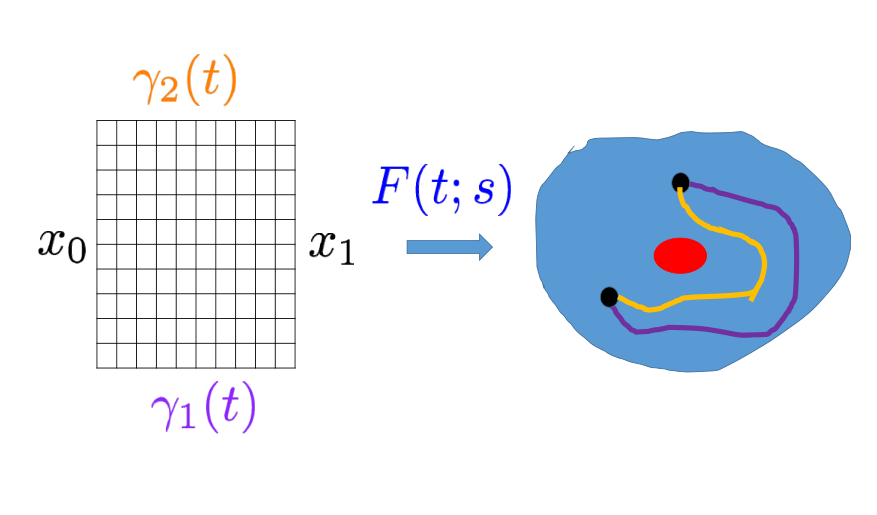
\includegraphics[width=0.72\textwidth]{figures/fig35.png}
  \caption{用图示说明下述论证：在 $\mathbb{C}$ 的一个区域上，平坦联络的平行移动只依赖固定端点曲线所在的同伦类。
  利用该同伦，把两条曲线之间的区域划分成小块：只需把同伦的定义域剖分成足够小的方块。
  于是绕每个小方块的单值性由联络及其协变导数算出，而这些全都为零。（原文 Fig.~35，第 207 页）}
  \label{fig:35}
\end{figure}

\textbf{例 3}\quad 设 $B$ 是 $\mathbb{C}$ 中的开连通区域。例如 $B$ 可以是
$\mathbb{C}-\{z_1,\dots,z_m\}$，即 $\mathbb{C}$ 去掉某组点。我们也可以把它看成扩充复平面再去掉
无穷远点：$B=\mathbb{C}P^1-\{z_1,\dots,z_m,\infty\}$。因此当 $m\ge 1$ 时它绝对不单连通。
再令 $E=B\times\mathbb{C}^n$，其中 $n$ 为某正整数。$B$ 中的路径可以用 $z(t)$ 表示。我们的路径提升规则
与例 1 类似：在 $B$ 上选取一对 $n\times n$ 矩阵值函数，记作 $(A_z,A_{\bar z})$，其中这一对里的每个矩阵
都是 $(z,\bar z)$ 的单值非奇异函数。\footnote{我们并不假定复共轭 $(A_z)^*$ 与 $A_{\bar z}$ 之间有任何关系。}
于是提升路径将是 $(z(t),\vec{v}(t))$，其中微分方程现在为：

\begin{equation}
  \frac{d}{dt}\vec{v}(t) + \left(A_z(z(t),\bar z(t))\frac{dz}{dt}
  + A_{\bar z}(z(t),\bar z(t))\frac{d\bar z}{dt}\right)\vec{v}(t) = 0
  \qquad \vec{v}(0)=\vec{v}_0.
  \tag{H.23}
  \label{eq:H.23}
\end{equation}

我们同样可以用路径排序指数「解出」这个微分方程，同样会有相当有趣的单值性。注意我们把两项放在了
方程的同一侧（因而这里的 $A$ 与前几个例子相差一个符号翻转）。这一符号约定最终更有用。

作为单值性的例子，让我们考虑以 $z_0$ 为基点的小环路，写成 $z(t)=z_0+\epsilon(t)$，其中对固定的 $t$，
复数 $\epsilon(t)$ 取得很小。特别地，该环路是同伦平凡的，于是存在以 $z_0$ 为基点的、使 $\partial D$
为 $\wp$ 的像的小圆盘 $D$。此时 $\mathbb{U}(\wp)$ 的首个非平凡贡献出现在 $\mathcal{O}(\epsilon^2)$ 阶，
并且可以证明

\begin{equation}
  \mathbb{U}(\wp) = 1 + \alpha F_{z\bar z}(z_0,\bar z_0) + \mathcal{O}(\epsilon^3)
  \tag{H.24}
  \label{eq:H.24}
\end{equation}

其中

\begin{equation}
  \alpha = \int_0^1 dt\,\dot{\epsilon}(t)\bar{\epsilon}(t)
  \tag{H.25}
  \label{eq:H.25}
\end{equation}

是（$(2i)$ 倍的）以 $z_0$ 处小环路所围的欧氏面积，而

\begin{equation}
  F_{z\bar z} := \partial_z A_{\bar z} - \partial_{\bar z}A_z + [A_z,A_{\bar z}]
  \tag{H.26}
  \label{eq:H.26}
\end{equation}

看清 $\alpha$ 正比于环路所围面积的一个办法是把它写成

\begin{equation}
  \alpha = \oint_\wp d\epsilon\,\bar{\epsilon} = \int_D d\epsilon\wedge d\bar{\epsilon}
  \tag{H.27}
  \label{eq:H.27}
\end{equation}

而后一个积分是环路所围欧氏面积的 $2i$ 倍。可以证明：在 \eqref{eq:H.24} 按 $\epsilon(t)$ 的幂作完整展开时，
所有项都只涉及 $\mathbb{F}_{z\bar z}$ 及其（协变）导数的乘积。

% [Tutor Note: (H.24) 与 (H.31) 的符号相反不要当成矛盾，(H.24) 的 $+$ 与 (H.31) 的 $-$ 来自
%  (H.23) 把两项移到方程同侧、即 $A$ 相对例 1 差一个符号，而 (H.29) 又沿用了 (H.23) 的约定；
%  核对时请从 (H.23) 的 $+\dot{v}+A\dot{x}v=0$ 出发重算一遍 $\epsilon$ 的一阶展开，否则很容易
%  把 $F$ 的整体符号搞反。另外 (H.25) 的 $\alpha$ 只取了「面积」的一阶项，
%  $\oint d\epsilon\,\bar\epsilon$ 与 $\int_D d\epsilon\wedge d\bar\epsilon$ 相差一个由 Stokes 定理
%  保证的边界项，故 $\alpha=2i\cdot\text{面积}$ 成立的前提是 $D$ 上 $\epsilon$ 单值。
%  另外 (H.32) 中 $[A_\mu,A_\nu]$ 的次序也必须与 $\partial_\mu A_\nu-\partial_\nu A_\mu$
%  的反对称性一致：把两项同时反号（$\mu\leftrightarrow\nu$）才自洽，别只改其中一项。]

% 说明：原文这一句写的是 "all the terms involve products of $\mathbb{F}_{z\bar z}$"，
%  用的是黑板粗体 $\mathbb{F}$ 而不是 $F$；这是作者笔误（同一页 (H.26) 用的是 $F_{z\bar z}$），
%  此处照原样转写，阅读时按 $F_{z\bar z}$ 理解。

{\small\itshape ［原文标记：这一点需要更充分地论证。］}

% [原文待办标记，原文 p.208 右侧页边 \ensuremath{\clubsuit}Need to justify that more fully. \ensuremath{\clubsuit}]

表达式 $F_{z\bar z}$ 称为该联络的曲率（curvature）。更恰当地，应把它看成本地矩阵值的 2-形式
$F=F_{z\bar z}dz\wedge d\bar z$。

有一类特别重要的联络是\emph{平坦联络}（flat connection），定义为曲率为零的联络。此时，给定平坦联络，
闭路的单值性矩阵 $\mathbb{U}(\wp)$ 只依赖 $\wp$ 在 $B$ 中的同伦类。用 \eqref{eq:H.24} 与路径复合性质很容易
证明这一点。由 \eqref{eq:H.24}，绕小环路的单值性必须是平凡的。而若 $F(t;s)$ 是从闭路 $\wp_1(s)$ 到
$\wp_2(s)$ 的同伦，则我们可以把方块 $I^2$ 剖分成许多小方块，绕每个小方块的单值性都必须是平凡的，
因此绕整个方块的单值性也必须是平凡的。于是 $\mathbb{U}(\wp_1\star\bar{\wp}_2)=1$，从而
$\mathbb{U}(\wp_1)=\mathbb{U}(\wp_2)$。

{\small\itshape ［原文标记：需要更多解释］}

% [原文待办标记，原文 p.208 右侧页边 \ensuremath{\clubsuit}Need more explanation \ensuremath{\clubsuit}；正文该句「绕每个小方块的
%  单值性都必须是平凡的」的前提是小方块内部没有奇点，这正是「平坦」的用处，作者未明说。]

在 $A_{\bar z}=0$ 且 $A_z$ 是 $z$ 的全纯函数这一特殊情形下，「$\mathbb{U}(\wp)$ 只依赖同伦类」
这一性质可以直接从路径排序指数看出来：

\begin{equation}
  \begin{aligned}
    \mathbb{U}(\wp_t) = {}& 1 + \int_{z_0}^{z(t)} A(z_1)dz_1 \\
    &+ \sum_{n=2}^{\infty}\int_{z_0}^{z(t)} dz_1\int_{z_0}^{z_1}dz_2\cdots\int_{z_0}^{z_{n-1}}dz_n\,
      A(z_1)\cdots A(z_n)
  \end{aligned}
  \tag{H.28}
  \label{eq:H.28}
\end{equation}

而此时该断言由 Cauchy 定理推出。这里 $dz_i$ 是 $\dot{z}(t_i)dt_i$ 等的简写。

\begin{figure}[htbp]
  \centering
  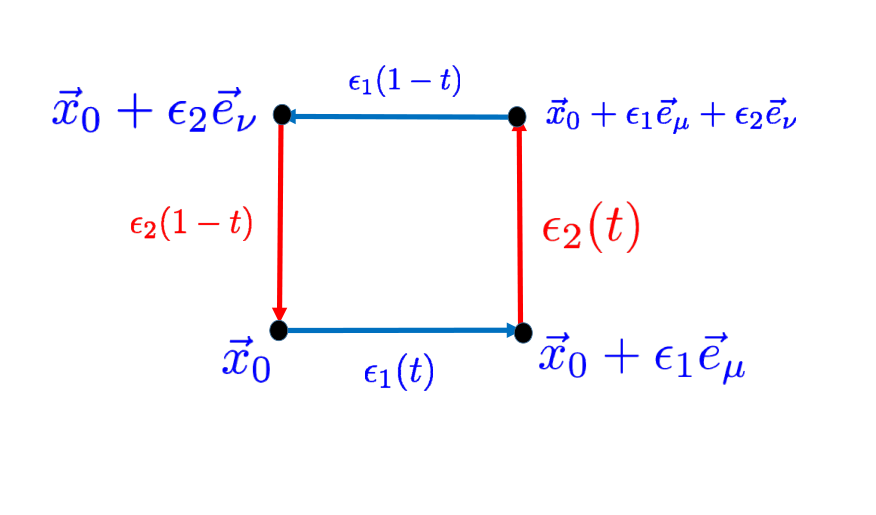
\includegraphics[width=0.60\textwidth]{figures/fig36.png}
  \caption{当 $\epsilon_1$ 与 $\epsilon_2$ 很小时，单值性的全部贡献都来自联络的曲率，
  其首项由环路的面积乘以 $\vec{x}_0$ 处由该环路（在切空间中）张成的平面内的曲率分量决定。
  （原文 Fig.~36，第 209 页）}
  \label{fig:36}
\end{figure}

\textbf{例 4}\quad 现在取 $B$ 为 $\mathbb{R}^m$ 中的开区域（$m>0$ 任意），$E=B\times\mathbb{C}^N$，
其中 $m$ 与 $N$ 一般完全无关。在 $\mathbb{C}^N$ 上取坐标 $x^\mu$，$\mu=1,\dots,m$，并令 $A_\mu(x)$
是 $B$ 上 $m$ 个复 $N\times N$ 矩阵值函数。我们假定它们单值且非奇异。与上面几个例子非常类似，
这些数据足以在由到第一个因子的投影给出的纤维化 $p:E\to B$ 上定义一个联络：设
$\wp:[0,1]\to B$ 是 $B$ 中从 $\vec{x}_0$ 到 $\vec{x}_1$ 的（分段可微）路径。然后我们在 $\vec{x}_0$
上方的纤维中选取提升 $(\vec{x}_0,\vec{v}_0)\in E$，并求解微分方程

\begin{equation}
  \frac{d}{dt}\vec{v}(t) + A_\mu(\vec{x}(t))\frac{dx^\mu(t)}{dt}\vec{v}(t) = 0
  \qquad \vec{v}(0)=\vec{v}_0
  \tag{H.29}
  \label{eq:H.29}
\end{equation}

而 $\mathbb{P}(\wp)(t)=(\vec{x}(t),\vec{v}(t))$ 就是提升。一般地会有有趣的单值性，甚至在任意点
$\vec{x}_0$ 附近的同伦平凡小路径上就已经出现。相关表达式是 \eqref{eq:H.24} 与 \eqref{eq:H.26} 的简单推广。确实，
任何无穷小曲线都可以看成落在某个过 $\vec{x}_0$ 的平面内，于是只需从复坐标换回实坐标即可。
或者，我们可以考虑由绕过 $x^\mu$-$x^\nu$ 平面内一个方形的四条开路径复合而成的小路径：

\begin{equation}
  \begin{aligned}
    \wp_1(t) &= \vec{x}_0 + \epsilon_1(t)\vec{e}_\mu \\
    \wp_2(t) &= (\vec{x}_0 + \epsilon_1\vec{e}_\mu) + \epsilon_2(t)\vec{e}_\nu \\
    \wp_3(t) &= (\vec{x}_0 + \epsilon_2\vec{e}_\nu) + \epsilon_1(1-t)\vec{e}_\mu \\
    \wp_4(t) &= \vec{x}_0 + +\epsilon_2(1-t)\vec{e}_\nu
  \end{aligned}
  \tag{H.30}
  \label{eq:H.30}
\end{equation}

% [Tutor Note: (H.30) 第四行原文多打了一个加号（$\vec{x}_0++\epsilon_2(1-t)\vec{e}_\nu$），
%  是排版笔误，此处照原样保留，数学上应读作 $\vec{x}_0+\epsilon_2(1-t)\vec{e}_\nu$。
%  另外 $\wp_4$ 的终点必须回到 $\vec{x}_0$ 才能闭合，故该行里的 $+ +$ 若按字面理解会破坏闭合性，
%  这也印证它是笔误。]

于是 $\wp=\wp_1\star\wp_2\star\wp_3\star\wp_4$。这里 $\vec{e}_\mu$ 是指向 $x^\mu$ 方向的单位向量，
而 $\epsilon_i:=\epsilon_i(t=1)$。见图 36。一个简单的计算表明 \eqref{eq:H.24} 与 \eqref{eq:H.26} 被推广为

\begin{equation}
  \mathbb{U}(\wp) = 1 - \epsilon_1\epsilon_2 F_{\mu\nu}(\vec{x}_0) + \cdots
  \tag{H.31}
  \label{eq:H.31}
\end{equation}

\begin{equation}
  F_{\mu\nu} := \partial_\mu A_\nu - \partial_\nu A_\mu + [A_\mu,A_\nu]
  \tag{H.32}
  \label{eq:H.32}
\end{equation}

而 \eqref{eq:H.31} 中的高阶项都是 $\epsilon_1^a\epsilon_2^b$ 阶的，其中 $a>0$、$b>0$、$a+b>2$。

\textbf{注}：可以证明，\eqref{eq:H.31} 中高阶项的系数是 $F_{\mu\nu}$ 及其沿 $\mu$ 与 $\nu$ 方向的协变导数的
多项式。一般地，任一矩阵值函数 $\Phi(x)$ 沿 $\lambda$ 方向的协变导数为

\begin{equation}
  D_\lambda\Phi := \partial_\lambda\Phi + [A_\lambda,\Phi]
  \tag{H.33}
  \label{eq:H.33}
\end{equation}

{\small\itshape ［原文标记：这一点有简单证明吗？或者有生成该级数的办法吗？我猜它是
$e^{\epsilon_1 D_\mu}e^{\epsilon_2 D_\nu}e^{-\epsilon_1 D_\mu}e^{-\cdots}$］}

% [原文待办标记，原文 p.210 右侧页边 \ensuremath{\clubsuit}Is there a simple proof of that? Or a way to generate
%  the series? I am guessing it is e^{ε1D_μ}e^{ε2D_ν}e^{-ε1D_μ}e^{-…} \ensuremath{\clubsuit} —— 作者的猜测正是
%  把 (H.30) 的方形环路写成四个平行移动算符的乘积，再作 BCH 展开。]

% 说明：(H.31) 里的负号与 (H.24) 里的正号之所以不同，见 (H.23) 之后的说明；若按例 1 的
%  约定 $\dot{v}=A\dot{x}v$（无负号）重算 (H.30) 的方形环路，得到的是
%  $\mathbb{U}=1+\epsilon_1\epsilon_2F_{\mu\nu}$。

\paragraph{练习}
对 $B=\mathbb{C}^*$、$N=1$、$A_z=\frac{\mu}{z}$、$A_{\bar z}=0$ 求解 \eqref{eq:H.23}，其中 $\mu$ 是复数。
计算该联络绕 $B$ 中某些简单闭路的单值性。

\paragraph{练习}
给出方程 \eqref{eq:H.24}、\eqref{eq:H.26}、\eqref{eq:H.31} 与 \eqref{eq:H.32} 的仔细推导。

\paragraph{练习}
证明：若矩阵 $A_\mu(x)$ 是反 Hermite 的，即 $(A_\mu(x))^{\dagger}=-A_\mu(x)$，则

\begin{equation}
  \mathrm{Pexp}\int_0^t A_\mu(x(t_1))\frac{dx^\mu}{dt_1}dt_1
  \tag{H.34}
  \label{eq:H.34}
\end{equation}

是酉的。

\paragraph{练习：规范变换}
设 $A(x)$ 是 $\mathbb{R}$ 上取值 $n\times n$ 复矩阵的矩阵值函数，而 $x\mapsto g(x)$ 是从 $\mathbb{R}$
到 $GL(n,\mathbb{C})$ 的可微映射。用

\begin{equation}
  A(x) = g(x)^{-1}\widetilde{A}(x)g(x) + g(x)^{-1}\frac{d}{dx}g(x)
  \tag{H.35}
  \label{eq:H.35}
\end{equation}

定义一个矩阵值函数 $\widetilde{A}(x)$。

% 说明：该练习的 a.)--f.) 各小问在下一页（印刷第 211 页），属下一片段；本片段止于 (H.35)。

% =====================================================================
%  c26 —— 原文印刷页 211--222（PDF 第 212--223 页）
%  内容：附录 I（I. Chern-Weil Theory And Chern-Simons Forms）
%        I.1 特征类；I.2 基本形式；I.3 Lie 代数上的不变多项式（I.3.1 例子）；
%        I.4 Chern-Weil 同态；I.5 对联络的依赖：特征类的构造；
%        I.6 Borel 定理；I.7 次级特征类：Chern-Simons 形式
%  编号公式：I.1--I.54 共 54 条（多行者为 I.5、I.16、I.19、I.20、I.22、
%        I.33、I.42、I.46、I.47、I.49、I.52）。
%  插图：Figure 37（第 220 页）、Figure 38（第 221 页）。原 PDF 中两图均为
%        空白占位框（figures/fig37.png、fig38.png 亦为空白），故按 main.tex
%        中既定的 \MissingFigureNote 方案处理：保留图号与图注，不插入空白图。
%  原文印刷页 211 上半页为附录 H 习题（H.36--H.40）的续页，属上一片段范围，
%  本片段按约定自 \section 级附录 I 开始。
% =====================================================================

\section{Chern-Weil 理论与 Chern-Simons 形式} % 原文: I. Chern-Weil Theory And Chern-Simons Forms

\begin{keytakeaways}
  \item 特征类是主丛同构类的函数：$\xi$ 把以 $G$ 为结构群的主丛 $P\to M$ 送到整上同调类
    $\xi(P)\in H^*(M;\mathbb{Z})$，并要求自然的拉回性质 \eqref{eq:I.1}；等价地，它来自分类空间
    的上同调类 $\theta\in H^*(BG;\mathbb{Z})$ 沿分类映射的拉回 $\xi(P)=f^*(\theta)$。
  \item Chern-Weil 构造：给定联络 $\Theta$ 与 Lie 代数上的不变多项式 $\varphi$（次数 $k$），把曲率
    $\bar F\in\Omega^2(P;\mathfrak{g})$ 代入得 $2k$ 次形式 $\varphi(\bar F)=\pi^*(\bar\varphi)$；它是基本
    形式且闭，故给出分次环同态 $I^*(G)\to H^*_{DR}(M)$，即 Chern-Weil 同态。
  \item 与联络无关：沿联络空间中任一路径 $A(t)$ 积分，两个联络处的特征形式之差是恰当形式
    \eqref{eq:I.20}、\eqref{eq:I.23}，因此上同调类与联络选取无关；在联络族上引入双分次与万有
    联络后，这一机制被整理成下降方程 \eqref{eq:I.42}。
  \item 次级特征类：把上述恰当形式中的原函数取出，便得相对 Chern-Simons 形式
    $CS_{2n-1}(A_1,A_0)$，它满足 $dCS_{2n-1}=\operatorname{Tr}F_1^n-\operatorname{Tr}F_0^n$。它本质上是
    「两个联络之间」的量，只有在平凡丛上取 $A_0=0$ 时才写作单个联络的 $CS(A)$；其积分只
    定义到模 $\mathbb{Z}$。
  \item Borel 定理：$H^*(BG;\Lambda)=(H^*(BT,\Lambda))^W$ 与 $I^*(G)=S^*(\mathfrak{g}^*)^W$ 给出
    $I^*(G)\cong H^*(BG;\mathbb{R})$，把不变多项式环、Weyl 群不变量与分类空间上同调三者闭合起来，
    这是 Chern-Weil 同态「取遍所有特征类」的根本原因。
\end{keytakeaways}

\subsection{特征类} % 原文: I.1 Characteristic classes

我们没有足够的篇幅来充分展开这个重要的主题。下面是电报式的简述。

粗略地说，特征类（characteristic class）是度量向量丛与主丛的扭曲（twisting）程度的一种办法。

按定义，特征类是一条把上同调类指派给主丛（的同构类）的规则。当 $\pi: P\to M$ 是以 $G$ 为结构群的主丛时，特征类是 $M$ 上的整上同调类。因此特征类是从 $M$ 上主丛的同构类集合到 $H^*(M;\mathbb{Z})$ 的映射。若 $P\to M$ 是主丛，我们用 $\xi(P)$ 记相应的上同调类。此外，这个映射应当是\emph{自然的}，即
\begin{equation}
  f^*(\xi(P)) = \xi(f^*(P))
  \tag{I.1}
  \label{eq:I.1}
\end{equation}

注意这样的特征类构成一个环。

由于性质 \eqref{eq:I.1}，特征类可以用分类空间 $BG$ 的上同调类来定义。若 $\theta\in H^*(BG;\mathbb{Z})$，而 $f: M\to BG$ 是 $P$ 的分类映射，即 $P=f^*(EG)$，则可取 $\xi(P)=f^*(\theta)$。而且所有特征类都是以这种方式得到的。

当丛 $P$ 上配有一个联络时，我们可以构造特征类的 DeRham 代表元。尽管这样做会丢失挠（torsion）信息，这一构造仍然非常有用，在物理中也极为常见。它导致 Yang-Mills 作用量中的拓扑项，并且通过所谓的次级特征类（即 Chern-Simons 形式），引出几何与物理相互作用中最有趣、最重要的许多例子。

\subsection{基本形式} % 原文: I.2 Basic forms

\textbf{定义} 丛 $P\to M$ 上的一个\emph{基本形式}（basic form）是指由底空间上的形式 $\tilde{\omega}$ 拉回而得的形式：$\omega=\pi^*(\tilde{\omega})$。

\textbf{命题.} 设 $P$ 是紧致连通群 $G$ 的主 $G$ 丛。则 $\omega\in\Omega^*(P)$ 是基本形式，当且仅当它满足
\begin{enumerate}[label=(\alph*)]
  \item $\iota(\xi(X))(\omega)=0$；
  \item $\mathcal{L}(\xi(X))(\omega)=0$，
\end{enumerate}
其中 $X$ 取遍 $\mathfrak{g}$。

\textbf{证明}：局部地取坐标 $(x,g)$。于是总空间上的任何形式都可以用 $dx^\mu$ 与 $e^a$ 展开，其中 $\Theta=e^aT_a$。

垂直性方程 $\iota(\xi(X))(\omega)=0$ 表示 $\omega$ 没有垂直分量。也就是说，在局部坐标下它具有如下形式：
\begin{equation}
  \omega = \omega_{\mu_1\cdots\mu_k}(x,g)\,dx^{\mu_1\cdots\mu_k}
  \tag{I.2}
  \label{eq:I.2}
\end{equation}

其次，Lie 导数条件表明系数函数必须与 $g$ 无关。\ $\clubsuit$

% [Tutor Note: 这里被略去的一步是：由 b) 得 $\mathcal{L}(\xi(X))\omega=0$，而 $\mathcal{L}=\iota d+d\iota$，把 (I.2) 代入并对 $g$ 沿单参数子群求导，即得 $\partial_g\omega_{\mu_1\cdots\mu_k}=0$（对连通 $G$ 而言 $g$ 可沿生成元方向走到单位元）。这正是不必额外假设「与 $g$ 无关」的原因，也说明了命题为何要假设 $G$ 紧致\emph{且连通}：对不连通群，(b) 只能保证在单位元分支上不变，故须换成 (I.3) 的 $R_g^*(\omega)=\omega$。]

\textbf{注}：更一般地，若 $G$ 不连通，则上面的条件 (b) 应表述为如下条件：
\begin{equation}
  R_g^*(\omega)=\omega \qquad \forall g\in G
  \tag{I.3}
  \label{eq:I.3}
\end{equation}

\subsection{Lie 代数上的不变多项式} % 原文: I.3 Invariant polynomials on the Lie algebra

设 $\mathfrak{g}$ 是 $\mathbb{F}=\mathbb{R}$ 或 $\mathbb{C}$ 上的 Lie 代数。$\mathfrak{g}$ 上的一个 $k$ 次多项式指的是一个全对称的多重线性函数：
\begin{equation}
  \varphi:\mathfrak{g}^{\otimes k}\to\mathbb{F}
  \tag{I.4}
  \label{eq:I.4}
\end{equation}

对称多项式是 $\mathrm{Sym}^k\mathfrak{g}^*$ 的元素，而 $\oplus_k\mathrm{Sym}^k\mathfrak{g}^*$ 合起来构成一个代数。次数分别为 $k_1,k_2$ 的两个多项式 $\varphi_1$ 与 $\varphi_2$ 的乘积是
\begin{equation}
\begin{aligned}
  (\varphi_1\cdot\varphi_2)(v_1,\dots,v_{k_1+k_2}) :={}&
    \frac{1}{(k_1+k_2)!}\sum_{\sigma\in S_{k_1+k_2}}
    \varphi_1(v_{\sigma(1)},\dots,v_{\sigma(k_1)})\\
  &\times \varphi_2(v_{\sigma(k_1+1)},\dots,v_{\sigma(k_1+k_2)})
\end{aligned}
  \tag{I.5}
  \label{eq:I.5}
\end{equation}

% [Tutor Note: 「$k$ 次多项式」在本文中始终指\emph{齐次}的对称多重线性函数，即 $\mathrm{Sym}^k\mathfrak{g}^*$ 中的元素，而不是通常意义下总次数为 $k$ 的多项式。核对 (I.5) 即知：两个齐次多项式之积仍是齐次的（次数相加），系数 $1/(k_1+k_2)!$ 正是把「有序的 $(k_1+k_2)$ 元组」对称化所需的归一化。作者在 (I.9) 处又用 "homogeneous of degree $k$" 这一说法，两者一致；若不注意这一点，(I.5) 前面的因子极易漏写。]

一个\emph{不变多项式}（invariant polynomial）是指 $Ad(G)$ 不变的多项式。不变多项式构成 $S^*(\mathfrak{g}^*)$ 的一个子环，记作 $I(G)^*$ 或 $\mathrm{Inv}_G S^*(\mathfrak{g})$。

\textbf{注}：不变多项式完全由它在对角线上的取值 $\varphi(v,v,\dots,v)$ 决定。证明：取一组基，用未定元 $x_i$ 把 $v=\sum v_ix_i$ 代入。我们将滥用记号，把这个对角值也记作 $\varphi(v)$。于是 $\varphi(gvg^{-1})=\varphi(v)$。

\textbf{定理} 若 $G$ 是紧致单 Lie 群，则不变多项式环是 Casimir 元上的多项式环
\begin{equation}
  \mathrm{Inv}_G S^*(\mathfrak{g}) \cong \mathbb{R}[C_1,C_2,\dots,C_\ell]
  \tag{I.6}
  \label{eq:I.6}
\end{equation}
其中 $\ell$ 是 $G$ 的秩，而 $C_i$ 的次数为 $k_i$，即 $G$ 的指数（exponents）。

\textbf{证明}：不变多项式由它在对角线上的值 $\varphi(v)$ 决定，而由 $Ad$-不变性，它又由在一个 Cartan 子代数 $\mathfrak{t}\subset\mathfrak{g}$ 上的取值决定。反之，$\mathfrak{t}$ 上任何 $W$-不变的多项式都定义了 $\mathfrak{g}$ 上的一个不变多项式，这里 $W$ 是 Weyl 群。由于 $W$ 是有限群，我们总可以把 $\mathfrak{t}$ 上的多项式取平均，从而得到一个 $W$-不变的多项式。结果表明，$W$-不变多项式环本身也是一个多项式环：见 C. Chevalley, ``Invariants of finite groups generated by reflections,'' Amer. J. Math. \textbf{77}(1955)778。\ $\clubsuit$

% [Tutor Note: 证明中 "It turns out that ..." 一句省略的是 Chevalley 定理（有限反射群的不变多项式环是多项式环，生成元的次数等于该群的指数）；这里 $W$ 是 $G$ 的 Weyl 群，它在 $\mathfrak{t}$ 上由单反射生成，故生成元 $C_i$ 的次数 $k_i$ 正是 $G$ 的指数。若要补全，可查 Humphreys《Reflection Groups and Coxeter Groups》第 3 章，或 Bourbaki《Lie Groups and Lie Algebras》第 V 章 §5。作者此处只给了一篇原始文献。]

\subsubsection{例子} % 原文: I.3.1 Examples

例 1：$Lie(GL(n,\mathbb{C}))=Mat_n(\mathbb{C})$。不变多项式环由 Chern 多项式 $C_k$ 生成，后者由下式定义：
\begin{equation}
  \det\left(xI+\frac{1}{2\pi i}A\right) = \sum_j C_j(A,\dots,A)\,x^{n-j}
  \tag{I.7}
  \label{eq:I.7}
\end{equation}

例 2：GL(n,R)

例 3：U(N)

例 4：$G=SO(2r)$……

对 $G=SO(2r)$，会出现一个新的重要不变多项式——Pfaffian：
\begin{equation}
  \mathrm{Pfaff}(m) = \frac{1}{2^r r!}\sum_{\sigma\in S_{2r}}\mathrm{sign}(\sigma)\,
  m_{\sigma(1)\sigma(2)}m_{\sigma(3)\sigma(4)}\cdots m_{\sigma(2r-1)\sigma(2r)}
  \tag{I.8}
  \label{eq:I.8}
\end{equation}
对于反对称矩阵而言，它是矩阵元的一个多项式，且满足 $(\mathrm{Pfaff}(m))^2=\det m$。

例 5：$G=SO(2r+1)$。

例 6：$G=USp(2r)$。

\paragraph{练习}
证明对任意 $g\in O(2r)$ 有 $\mathrm{Pfaff}(gmg^{-1})=\det(g)\,\mathrm{Pfaff}(m)$。

\subsection{Chern-Weil 同态} % 原文: I.4 The Chern-Weil homomorphism

现在设 $\pi: P\to M$ 是以 $G$ 为结构群的主丛，配有联络 $\Theta$ 与场强 $\bar F\in\Omega^2(P;\mathfrak{g})$。设 $\varphi$ 是 $\mathfrak{g}$ 上的一个不变多项式。

于是我们可以考虑
\begin{equation}
  \varphi(\bar F)
  \tag{I.9}
  \label{eq:I.9}
\end{equation}
若 $\varphi$ 是 $k$ 次齐次的，则 $\varphi(\bar F)$ 是 $P$ 上的 $2k$ 次微分形式。

一个应当记住的典型例子是某个表示 $\rho$ 下的迹：
\begin{equation}
  \varphi_{k,\rho}(\bar F) := \operatorname{Tr}_\rho \rho(\bar F)^k
  \tag{I.10}
  \label{eq:I.10}
\end{equation}
（下文我们将经常略去此记号中的 $\rho$。）

\textbf{命题}：形式 $\varphi(\bar F)=\pi^*(\bar\varphi)$ 是基本形式。

\textbf{证明} 显然 $\varphi(\bar F)$ 是水平的，即 $\iota(\xi(X))\varphi(\bar F)=0$，因为 $\iota(\xi(X))(\bar F)=0$。此外，
\begin{equation}
  R_g^*(\varphi(\bar F)) = \varphi(R_g^*(\bar F)) = \varphi(g\bar Fg^{-1}) = \varphi(\bar F)
  \tag{I.11}
  \label{eq:I.11}
\end{equation}
因而它沿纤维方向不变。\ $\clubsuit$

\textbf{命题}：$\bar\varphi(\bar F)$ 是底空间 $M$ 上的闭微分形式。而且它是自然的。

\textbf{证明} 注意：
\begin{equation}
  d\varphi(\bar F,\cdots,\bar F) = k\,\varphi(d\bar F,\bar F,\cdots,\bar F)
  \tag{I.12}
  \label{eq:I.12}
\end{equation}
但现在我们使用 Bianchi 恒等式
\begin{equation}
  D\bar F = d\bar F + [\Theta,\bar F] = 0
  \tag{I.13}
  \label{eq:I.13}
\end{equation}
现在注意 $\varphi([\Theta,\bar F],\bar F,\cdots,\bar F)=0$，因为 $\varphi$ 是 $Ad$-不变的。（回想 $\Theta$ 取值于 $\mathfrak{g}$，并利用 $Ad$-不变性的无穷小形式。）于是（在 DeRham 复形上！）$\pi^*$ 没有核，故 $d\bar\varphi(\bar F)=0$。\ $\clubsuit$

% [Tutor Note: (I.12) 的关键是对 $k$ 个相同的偶次因子 $\bar F$（每个 2 次）用 Leibniz 法则：$k$ 个因子各贡献一项、没有符号因子（因 $\bar F$ 是偶次形式），故系数为 $k$；再代入 (I.13) 得 $d\bar F=-[\Theta,\bar F]$。而 $\varphi([\Theta,\bar F],\bar F,\dots,\bar F)=0$ 用到的是 $Ad$-不变性的\emph{无穷小}形式：$\sum_{i}\varphi(\bar F,\dots,[\Theta,\bar F],\dots,\bar F)=0$，即 $\varphi$ 在 $\mathfrak{g}$ 上 $ad(\mathfrak{g})$-不变。此处作者只说「利用 $Ad$-不变性的无穷小形式」，跳过了这层等价性。]

为证明自然性：

注意若 $f: P_1\to P_2$ 是覆盖 $\bar f: M_1\to M_2$ 的丛映射，且 $\Theta_1=f^*(\Theta_2)$ 是拉回联络，则 $\varphi(\bar F_1)=f^*(\varphi(\bar F_2))$，从而 $\bar\varphi(\bar F_1)=\bar f^*(\bar\varphi(\bar F_2))$。特别地，$\bar\varphi(\bar F)$ 的上同调类只依赖于 $(P,\Theta)$ 的同构类。\ $\clubsuit$

最后注意，若 $\varphi$ 是 $k$ 次的，则 $\bar\varphi(\bar F)\in\Omega^{2k}(M)$ 是 $2k$ 次形式。此外，对称多项式的乘积对应上同调类的乘积。于是我们有如下定义：

\textbf{定义}：Chern-Weil 同态是分次环的同态
\begin{equation}
  I^*(G)\to H^*_{DR}(M)
  \tag{I.14}
  \label{eq:I.14}
\end{equation}
它把 $\varphi$ 送到 $[\bar\varphi(\bar F)]$。

\textbf{注}：

\begin{enumerate}
  \item 考虑 Hopf 纤维化上的自然联络。由于 $u(1)$ 是阿贝尔的，Lie 代数上任何多项式都是不变的。场强 $\bar F$ 是基本形式，它在 $S^2$ 底空间上有非平凡的积分。{\small\itshape ［原文标记：$\clubsuit$需要解释$\clubsuit$］}
  % [原文待办标记，原文 p.215 右侧边注；原文写作 "NEED TO EXPLAIN"]
  \item 理解「该形式是基本的」这一事实的另一条途径，是完全在底空间上用局部坐标卡来做。在每个坐标卡 $\mathcal{U}_\alpha$ 中，$\operatorname{Tr}F_\alpha^k$ 是规范不变的。因此，跨过坐标卡边界比较联络得 $F_\alpha=g_{\alpha\beta}F_\beta g_{\alpha\beta}^{-1}$，从而 $\operatorname{Tr}F_\alpha^k$ 实际上是 $M$ 上整体良定义的 $2k$ 形式。在下面的工作中，我们有时会直接用定义在底空间上的 $F$ 来工作。回想在局部坐标下 $\Theta=g^{-1}dg+g^{-1}Ag$，而 $\bar F=g^{-1}Fg$。
  \item 更一般地，任何规范不变的量，例如由联络构成的 Yang-Mills 作用量密度 $\operatorname{Tr}F*F$，都会在底空间上整体良定义。
\end{enumerate}

% [Tutor Note: 第 2 条中原文写作 "path boundaries"，从上下文及第 219 页练习中的 "patch boundaries" 判断应为 "patch boundaries"（坐标卡边界）；此处按后者译出。$F_\alpha=g_{\alpha\beta}F_\beta g_{\alpha\beta}^{-1}$ 之所以成立，是因为在重叠区 $\Theta_\alpha=g_{\alpha\beta}^{-1}\Theta_\beta g_{\alpha\beta}+g_{\alpha\beta}^{-1}dg_{\alpha\beta}$ 中规范势的那一项恰好抵消曲率，曲率只作张量式变换。]

\paragraph{练习}
设 $\alpha,\beta$ 是取值于 $\mathfrak{g}$ 的 $j$ 次与 $k$ 次微分形式。证明
\begin{equation}
  \boxed{\,d\operatorname{Tr}(\alpha\wedge\beta)
  = \operatorname{Tr}\left[D_A(\alpha)\wedge\beta+(-1)^k\alpha\wedge D_A(\beta)\right]\,}
  \tag{I.15}
  \label{eq:I.15}
\end{equation}
其中
\begin{equation}
\begin{aligned}
  D_A\alpha &= d\alpha+A\alpha-(-1)^k\alpha A\\
  D_A\beta &= d\beta+A\beta-(-1)^j\beta A
\end{aligned}
  \tag{I.16}
  \label{eq:I.16}
\end{equation}

利用此式与 Bianchi 恒等式，直接验证
\begin{equation}
  d\operatorname{Tr}F^k = k\operatorname{Tr}(D_AF)F^{k-1} = 0
  \tag{I.17}
  \label{eq:I.17}
\end{equation}

\subsection{对联络的依赖：特征类的构造} % 原文: I.5 Dependence on connection: Construction of characteristic classes

现在来看 Weil 同态的一个关键性质：它的像实际上并不依赖于 $P$ 上联络的选取。

下面我们证明上同调类 $[\bar\varphi(\bar F)]$ 实际上与 $P$ 上联络的选取无关。

让我们从主要的特殊情形开始，并在底空间上局部地进行。于是我们考察基本形式 $\operatorname{Tr}F^n$ 对联络选取的依赖。回想在无穷小变分下：
\begin{equation}
  \delta F = D_A(\delta A)
  \tag{I.18}
  \label{eq:I.18}
\end{equation}

因此
\begin{equation}
\begin{aligned}
  \delta\operatorname{Tr}F^n
  &= n\operatorname{Tr}(\delta F)F^{n-1}\\
  &= n\operatorname{Tr}\left(D_A(\delta A)F^{n-1}\right)\\
  &= n\,d\left(\operatorname{Tr}\delta A\,F^{n-1}\right)
\end{aligned}
  \tag{I.19}
  \label{eq:I.19}
\end{equation}
其中我们用了 Bianchi 恒等式 $D_AF=0$。

更形式化地，若我们有一条\emph{线性}的联络路径：$A(t)=(1-t)A_0+tA_1=A_0+t\alpha$，$\alpha\in\Omega^1(M;\mathrm{ad}P)$，则
\begin{equation}
\begin{aligned}
  \operatorname{Tr}F_1^n-\operatorname{Tr}F_0^n
  &= \int_0^1 dt\,\frac{d}{dt}\operatorname{Tr}F(A(t))^n\\
  &= n\int_0^1 dt\,\operatorname{Tr}D_{A(t)}(\alpha)F(A(t))^{n-1}\\
  &= d\left[n\int_0^1 dt\,\operatorname{Tr}\alpha\,F(A(t))^{n-1}\right]\\
  &= d\left[n\int_0^1 dt\,\operatorname{Tr}\alpha\left(F_0+tD_{A_0}\alpha+t^2\alpha^2\right)^{n-1}\right]
\end{aligned}
  \tag{I.20}
  \label{eq:I.20}
\end{equation}

注意表达式
\begin{equation}
  n\int_0^1 dt\,\operatorname{Tr}\alpha\left(F_0+tD_{A_0}\alpha+t^2\alpha^2\right)^{n-1}
  \tag{I.21}
  \label{eq:I.21}
\end{equation}
是\emph{整体良定义}的，因为它只涉及张量性的量。因此，$M$ 上闭且整体良定义的形式 $\operatorname{Tr}F(A)^n$ 的 DeRham 上同调类与联络无关。

% [Tutor Note: (I.20) 第三行到第四行的替换是极易出错的一步：需先写出 $F(A(t))=d(A_0+t\alpha)+(A_0+t\alpha)^2=F_0+tD_{A_0}\alpha+t^2\alpha^2$，其中 $D_{A_0}\alpha=d\alpha+[A_0,\alpha]$；再把 $D_{A(t)}(\alpha)=D_{A_0}\alpha+2t\alpha^2$ 代回上一行，用 $\operatorname{Tr}$ 的循环性与 $D_{A_0}$ 下分部积分（$\int_0^1 dt\,d/dt(\cdot)$ 与 $\operatorname{Tr}\alpha\,d(\cdot)$ 的对易）把 $d$ 提到积分号外。作者只写了结果；核对时可用 $n=1$（此时 $F_0+tD_{A_0}\alpha+t^2\alpha^2$ 的零次幂为 $1$，退化为 $\operatorname{Tr}\alpha$）与 $n=2$ 两个情形验证系数。]

同样的运算对任意 $n$ 次不变多项式都成立：
\begin{equation}
\begin{aligned}
  \frac{d}{dt}\varphi(F(A(t)))
  &= n\,\varphi(D_{A(t)}\alpha,F(A(t)),\dots,F(A(t)))\\
  &= n\,d\Big(\varphi(\alpha,F(A(t)),\dots,F(A(t)))\Big)
\end{aligned}
  \tag{I.22}
  \label{eq:I.22}
\end{equation}
积分给出
\begin{equation}
  \varphi(F(A_1))-\varphi(F(A_0))
  = d\left[n\int_0^1\varphi(\alpha,F(A(t)),\dots,F(A(t)))\right]
  \tag{I.23}
  \label{eq:I.23}
\end{equation}
从而上同调类不变。

正如我们已经证明的，$[\bar\varphi(F)]$ 是自然的；因此，给定不变多项式 $\varphi$，我们可以按如下规则产生一个特征类：
\begin{equation}
  \xi: P\to[\bar\varphi(F)]
  \tag{I.24}
  \label{eq:I.24}
\end{equation}

其中我们可以使用 $P$ 上的任何联络。也就是说，Chern-Weil 同态与联络无关。

\textbf{注}：由此可知，闭链上的积分（包括 $M$ 闭时整个流形上的积分）都是「拓扑不变量」。这正是 Yang-Mills 作用量中许多拓扑项的来源。

\subsection{Borel 定理} % 原文: I.6 The Borel Theorem

现在我们可以把这一圈想法闭合起来：借助 Borel 定理，把不变多项式与分类空间的上同调联系起来：

\textbf{定理.} 设 $G$ 是紧致连通 Lie 群。则
\begin{equation}
  H^*(BG;\Lambda) = \left(H^*(BT,\Lambda)\right)^W
  \tag{I.25}
  \label{eq:I.25}
\end{equation}
其中 $W$ 是 Weyl 群，$T$ 是极大环面，$\Lambda$ 是任一使 $|W|$ 在其中可逆的环。

上标 $W$ 表示我们取 Weyl 群作用下的不变量。

若 $\Lambda=\mathbb{R}$，则我们可以用 Lie 代数上的 $Ad$-不变多项式来构造这个环：
\begin{equation}
  I^*(G) = S^*(\mathfrak{g}^*)^W
  \tag{I.26}
  \label{eq:I.26}
\end{equation}

于是

\textbf{定理}：若 $G$ 是紧致 Lie 群，则
\begin{equation}
  I^*(G)\cong H^*(BG;\mathbb{R})
  \tag{I.27}
  \label{eq:I.27}
\end{equation}

Borel 定理的参考文献：

\begin{enumerate}
  \item A. Borel, ``Topology of Lie Groups and Characteristic Classes,'' Bull. Amer. Math. Soc. \textbf{61}(1955) 397
  \item J. Dupont, \emph{Curvature and Characteristic Classes}, Lecture Notes in Mathematics \textbf{640} Springer 1978
\end{enumerate}

{\small\itshape ［原文标记：*******************\newline
讨论问题：若所有特征类都平凡，丛是否平凡？\newline
特征类的正确整归一化！！！！！\newline
*******************］}
% [原文待办标记，原文 p.217（印刷页），作者以星号行框住两句待办；原文为 "Discuss the question: If all the characteristic classes are trivial is the bundle trivial? / PROPER INTEGRAL NORMALIZATIONS OF THE CLASSES!!!!!"]

\subsection{次级特征类：Chern-Simons 形式} % 原文: I.7 Secondary characteristic classes: The Chern-Simons forms

让我们回到表达式：
\begin{equation}
  \varphi(F(A_1))-\varphi(F(A_0))
  = d\left[n\int_0^1 dt\,\varphi(\alpha,F(A(t)),\dots,F(A(t)))\right]
  \tag{I.28}
  \label{eq:I.28}
\end{equation}
它给出了 Chern-Weil 形式对联络选取的依赖。下面我们将更细致地考察那些使这一差别变为平凡的形式。为简单起见，我们把 $\varphi$ 取为 $\mathfrak{g}$ 的某个表示下的迹。

\emph{次级特征类}（secondary characteristic class）由使这一差别变为平凡的形式来定义：

\textbf{定义.} 两个联络之间的\emph{相对 Chern-Simons 形式}是如下形式：
\begin{equation}
  CS_{2n-1}(A_1,A_0) := n\int_0^1 dt\,\operatorname{Tr}\alpha
  \left(F_0+tD_{A_0}\alpha+t^2\alpha^2\right)^{n-1}
  \tag{I.29}
  \label{eq:I.29}
\end{equation}
其中 $A_1=A_0+\alpha$。

注意
\begin{equation}
  dCS_{2n-1}(A_1,A_0) = \operatorname{Tr}F_1^n-\operatorname{Tr}F_0^n
  \tag{I.30}
  \label{eq:I.30}
\end{equation}

\textbf{例}

\begin{equation}
  CS_1(A_1,A_0) = \operatorname{Tr}\alpha
  \tag{I.31}
  \label{eq:I.31}
\end{equation}

\begin{equation}
  CS_3(A_1,A_0) = \operatorname{Tr}\left(2\alpha F_0+\alpha D_{A_0}\alpha+\frac{2}{3}\alpha^3\right)
  \tag{I.32}
  \label{eq:I.32}
\end{equation}

\begin{equation}
\begin{aligned}
  CS_5(A_1,A_0) = \operatorname{Tr}\Big(&
    3\alpha F_0^2+\frac{3}{2}\alpha\{F_0,D_{A_0}\alpha\}+2F_0\alpha^3\\
  &+\alpha(D_{A_0}\alpha)^2+\frac{3}{2}\alpha^3D_{A_0}\alpha+\frac{3}{5}\alpha^5\Big)
\end{aligned}
  \tag{I.33}
  \label{eq:I.33}
\end{equation}

% [Tutor Note: 归一化最容易出错。(I.32) 中 $\alpha$ 的一次项系数 2、三次项系数 $2/3$ 都来自 (I.29) 对 $t$ 的积分：$n=2$ 时 $(F_0+tD_{A_0}\alpha+t^2\alpha^2)$ 的一次幂对 $t$ 积分给出 $F_0+\tfrac12 D_{A_0}\alpha+\tfrac13\alpha^2$，再乘以外面的 $n=2$ 即得 (I.32)。最省事的核对办法是取 $A_0=0$、$\alpha=A$，验证 $dCS_3=\operatorname{Tr}F^2$，即 $d\operatorname{Tr}(A\,dA+\tfrac23A^3)=\operatorname{Tr}(dA+A^2)^2$；若把系数写成 $1/3$ 或 $1/2$ 此式即不成立。]

\textbf{注}

\begin{enumerate}
  \item 通常 Chern-Simons 形式是用单个联络 $A$ 来表示的。当 $A$ 是平凡丛上的联络时，这样做是有意义的：此时可在上面所有公式中取 $A_0=0$、$A_1=A$。许多物理文献在这一点上非常马虎，当 $A$ 是非平凡联络时也写成 $CS(A)$。这种马虎会导致错误。务必小心！{\small\itshape ［原文标记：$\clubsuit$好吧。如果你取指数映射，那么对单个联络你\emph{确实}可以定义，而且这对后面各讲余下的内容很重要！！！$\clubsuit$］}
  % [原文待办标记，原文 p.218 右侧边注；原文写作 "Well. If you exponentiate, then you CAN define for a single connection, and this is important to the rest of the lectures !!!"]
  \item 话虽如此，确实有一种办法把 Chern-Simons 形式 $CS(A)$ 对单个联络定义为全空间上的良定义形式，即主丛 $P\to M$ 的全空间上的形式，因为联络形式在 $P$ 的全空间上是整体良定义的。更详细的讨论见 [22] 的附录 A。{\small\itshape ［原文标记：$\clubsuit$为什么 Dan 要用这个更复杂的论证？$\clubsuit$］}
  % [原文待办标记，原文 p.218 右侧边注；原文写作 "Why does Dan use this more complicated argument?"，Dan 指 D. Freed]
  \item 然后我们可以这样来定义 Chern-Simons 作用量：远离一个零测集选取截面 $s: M\to P$，并定义 $\int_M s^*CS(A)$。这将是不确定的，因为我们可以选取不同的截面，因此 $\int_M s^*CS(A)$ 只定义到模 $\mathbb{Z}$ 为止。
  \item 警告：在许多应用中，Chern-Simons 形式只被看作定义到恰当形式为止。注意 $CS\to CS+d(*)$ 不改变关键性质 \eqref{eq:I.20}。
\end{enumerate}

\paragraph{练习}
注意当 $M$ 不闭时，$\int_M\operatorname{Tr}F^n$ 依赖于联络。

\paragraph{练习}
证明：
\begin{equation}
  CS_3(A+\alpha+\beta,A)
  = CS_3(A+\alpha,A)+CS_3(A+\alpha+\beta,A+\alpha)-d(\operatorname{Tr}\alpha\beta)
  \tag{I.34}
  \label{eq:I.34}
\end{equation}
特别地：
\begin{equation}
  \frac{d}{dt}CS(A+\alpha(t),A)
  = 2\operatorname{Tr}\dot{\alpha}\big(F(A+\alpha)\big)-d(\operatorname{Tr}\alpha\dot{\alpha})
  \tag{I.35}
  \label{eq:I.35}
\end{equation}
这常被写成：
\begin{equation}
  \delta CS(A) = 2\operatorname{Tr}\delta A\wedge F(A)-d\big(\operatorname{Tr}(A\,\delta A)\big)
  \tag{I.36}
  \label{eq:I.36}
\end{equation}
这里假定丛是平凡的。

特别地，考虑 3 维流形 $M$ 上的主 $G$ 丛。「Chern-Simons 作用量」
\begin{equation}
  \int_M \operatorname{Tr}A\,dA+\frac{2}{3}A^3
  \tag{I.37}
  \label{eq:I.37}
\end{equation}
的变分是什么？

\paragraph{练习}
计算跨越坐标卡边界时 $CS_3(A_\alpha)-CS_3(A_\beta)$ 的变分。

\paragraph{练习}
证明 $CS(A_1^g,A_0^g)=CS(A_1,A_0)$。

现在让我们考察 Chern-Simons 形式本身对 $A$ 的依赖。

下面这个一般性的注记很有用：假设我们有一族联络 $A(s,x)$，记该族所在的空间为 $\mathcal{S}$。在 $\Omega^{p,q}(M\times\mathcal{S})$ 上引入双分次是有用的，使得 $(p,q)$ 形式属于 $\Omega^p(M)\otimes\Omega^q(\mathcal{S})$。我们可以在 $\pi^*P\to M\times\mathcal{S}$ 上构造一个联络 $\mathcal{A}(s,x)$，使其协变导数为
\begin{equation}
  d_M+d_{\mathcal{S}}+A(s,x)
  \tag{I.38}
  \label{eq:I.38}
\end{equation}
注意该联络形式只有 $(1,0)$ 型分量。这是所谓的「万有联络」（universal connection）的一个例子。（关于这一点更多内容，见下文。）设 $\mathcal{F}$ 是这个万有联络的曲率。它具有 $(2,0)$ 型与 $(1,1)$ 型分量。具体地
\begin{equation}
  \mathcal{F} = F(\mathcal{A}) = F(A)+d_{\mathcal{S}}A(s,x)
  \tag{I.39}
  \label{eq:I.39}
\end{equation}
现在 $\operatorname{Tr}\mathcal{F}^n$ 在全空间上是闭的，
\begin{equation}
  (d_M+d_{\mathcal{S}})\operatorname{Tr}\mathcal{F}^n = 0,
  \tag{I.40}
  \label{eq:I.40}
\end{equation}
于是若按 $(p,q)$ 型分解：
\begin{equation}
  \operatorname{Tr}\mathcal{F}^n = \omega^{n,0}+\omega^{n-1,1}+\dots+\omega^{0,n}
  \tag{I.41}
  \label{eq:I.41}
\end{equation}
并令 $d=d_M$、$\delta=d_{\mathcal{S}}$，我们就得到「下降方程」（descent equations）：
\begin{equation}
\begin{aligned}
  d\omega^{n,0} &= 0\\
  d\omega^{n-1,1}+\delta\omega^{n,0} &= 0\\
  d\omega^{n-2,2}+\delta\omega^{n-1,1} &= 0\\
  &\ \ \vdots
\end{aligned}
  \tag{I.42}
  \label{eq:I.42}
\end{equation}

% [Tutor Note: 原 PDF 第 220 页的 Figure 37 为空白占位框，图形内容在原稿中缺失，仅存图注；此处按原图注翻译并保留图号，以免后文图号错位。]
\begin{figure}[htbp]
  \centering
  \MissingFigureNote
  \caption{$\mathcal{A}(P)$ 中由三个联络构成的三角形。（原文 Fig.~37，第 220 页；原 PDF 此图缺失）}
  \label{fig:37}
\end{figure}

现在让我们考虑联络的一个单形 $\triangle$：
\begin{equation}
  A_0+t_1\alpha_1+t_2\alpha_2
  \tag{I.43}
  \label{eq:I.43}
\end{equation}
其中 $0\le t_2\le t_1\le 1$，如图 \ref{fig:37} 所示。

令 $A_1=A_0+\alpha_1$，$A_2=A_1+\alpha_2$。我们在 $\pi^*(P)\to M\times\triangle$ 上构造万有联络并计算曲率：
\begin{equation}
  F(\mathcal{A}) = F(A_0)+t_1D_{A_0}\alpha_1+t_2D_{A_0}\alpha_2
  +(t_1\alpha_1+t_2\alpha_2)^2+dt_1\alpha_1+dt_2\alpha_2
  \tag{I.44}
  \label{eq:I.44}
\end{equation}

利用下降方程可以写出
\begin{equation}
  \int_\triangle\delta\omega^{n-1,1}
  = -d\int_\triangle\omega^{n-2,2}
  = -d\int_\triangle\operatorname{Tr}F(\mathcal{A})^n
  \tag{I.45}
  \label{eq:I.45}
\end{equation}
另一方面，我们可以对三角形应用 Stokes 定理，写出
\begin{equation}
\begin{aligned}
  \int_\triangle\delta\omega^{n-1,1}
  &= \int_{\partial\triangle}\omega^{n-1,1}
  = \int_{\partial\triangle}\operatorname{Tr}F(\mathcal{A})^n\\
  &= CS_{2n-1}(A_1,A_0)+CS_{2n-1}(A_2,A_1)+CS_{2n-1}(A_0,A_2)
\end{aligned}
  \tag{I.46}
  \label{eq:I.46}
\end{equation}
把它们放在一起，我们就得到结果：
\begin{equation}
\begin{aligned}
  &CS_{2n-1}(A_0,A_1)+CS_{2n-1}(A_1,A_2)+CS_{2n-1}(A_2,A_0)\\
  &\quad = d_M\Bigg(\int_\triangle \operatorname{SymTr}\Big(dt_1\alpha_1,\,dt_2\alpha_2,\,
    \big(F(A_0)+t_1D_{A_0}\alpha_1+t_2D_{A_0}\alpha_2+(t_1\alpha_1+t_2\alpha_2)^2\big)^{n-2}\Big)\Bigg)
\end{aligned}
  \tag{I.47}
  \label{eq:I.47}
\end{equation}

于是，例如：
\begin{equation}
  CS_3(A_1,A_0)+CS_3(A_2,A_1)+CS_3(A_0,A_2) = d(\operatorname{Tr}\alpha_1\alpha_2)
  \tag{I.48}
  \label{eq:I.48}
\end{equation}
其中 $A_1=A_0+\alpha_1$，$A_2=A_1+\alpha_2$。

类似地：
\begin{equation}
\begin{aligned}
  &CS_5(A_1,A_0)+CS_5(A_2,A_1)+CS_5(A_0,A_2) =\\
  &\quad 3d\left[\int_\triangle \operatorname{Tr}
    \big(F+t_1D\alpha_1+t_2D\alpha_2+(t_1\alpha_1+t_2\alpha_2)^2\big)(\alpha_1\alpha_2-\alpha_2\alpha_1)\right]
\end{aligned}
  \tag{I.49}
  \label{eq:I.49}
\end{equation}

% [Tutor Note: 原 PDF 第 221 页的 Figure 38 为空白占位框，图形内容在原稿中缺失，仅存图注；此处按原图注翻译并保留图号，以免后文图号错位。]
\begin{figure}[htbp]
  \centering
  \MissingFigureNote
  \caption{$\mathcal{A}(P)$ 中用来计算 Chern-Simons 形式 $CS(A,0)$ 的规范依赖性的联络三角形。（原文 Fig.~38，第 221 页；原 PDF 此图缺失）}
  \label{fig:38}
\end{figure}

作为一个应用，设 $A$ 是可平凡化丛上的一个联络，于是存在基点联络 $A_0=0$。这时定义 $CS(A):=CS(A,0)$ 是有意义的。虽然 $dCS(A)$ 是规范不变的，$CS(A^g)$ 却不是规范不变的。

在上面的公式中，我们可以取 $A_1=g^{-1}dg$、$A_2=A^g$，其中 $A$ 是某个整体定义的联络 1-形式。注意这意味着我们有一条从 $A_1$ 到 $A_2$ 的线性路径 $A(t)=g^{-1}dg+t\,g^{-1}Ag$。由于一般地 $CS(A_1^g,A_0^g)=CS(A_1,A_0)$ 对任意一对联络成立，我们有
\begin{equation}
  CS_{2n-1}(A^g,g^{-1}dg) = CS_{2n-1}(A,0)
  \tag{I.50}
  \label{eq:I.50}
\end{equation}

因此，我们的恒等式变成：
\begin{equation}
  CS_{2n-1}(A^g)-CS_{2n-1}(A) = CS_{2n-1}(g^{-1}dg)-d_M(\alpha_{2n})
  \tag{I.51}
  \label{eq:I.51}
\end{equation}
其中
\begin{equation}
\begin{aligned}
  \alpha_{2n} = \int_\triangle \operatorname{SymTr}\Big[&
    dt_1\alpha_1,\,dt_2\alpha_2,\,
    \Big((t_1^2-t_1)\alpha_1^2+(t_2^2-t_2)\alpha_2^2\\
  &+(t_1t_2-t_2)[\alpha_1,\alpha_2]_+ + t_2g^{-1}F(A)g\Big)^{n-2}\Big]
\end{aligned}
  \tag{I.52}
  \label{eq:I.52}
\end{equation}
这里 $\alpha_1=g^{-1}dg$、$\alpha_2=g^{-1}Ag$，以及
\begin{equation}
  CS_{2n-1}(g^{-1}dg) = (-1)^{n-1}\frac{n!\,(n-1)!}{(2n-1)!}
  \operatorname{Tr}(g^{-1}dg)^{2n-1}
  \tag{I.53}
  \label{eq:I.53}
\end{equation}

% [Tutor Note: (I.53) 的系数可直接由 (I.29) 核对：取 $A_0=0$、$\alpha=g^{-1}dg$，此时 $\alpha$ 平坦（$d\alpha+\alpha^2=0$），故 $F(A(t))=t\,d\alpha+t^2\alpha^2=t(t-1)\alpha^2$，(I.29) 化为 $n\int_0^1 t^{n-1}(t-1)^{n-1}dt\,\operatorname{Tr}\alpha^{2n-1}=(-1)^{n-1}\frac{n!\,(n-1)!}{(2n-1)!}\operatorname{Tr}\alpha^{2n-1}$，正是 (I.53)。最容易抄错的是 Beta 积分 $B(n,n)=(n-1)!^2/(2n-1)!$ 给出的 $(n-1)!^2$ 与 $(-1)^{n-1}$；用 $n=2$ 检验：$2\int_0^1 t(t-1)dt=2\cdot(-\tfrac16)=-\tfrac13$，与 $(-1)^{1}\frac{2!\,1!}{3!}=-\tfrac13$ 一致。]

这个公式在讨论带 Chern-Simons 项的物理作用量、以及诸如反常的下降形式体系（descent formalism）与「反常流入」（anomaly inflow）等话题时很有用。见下文。

也可以用「Cartan 同伦算子」的形式体系来导出它。见

\begin{enumerate}
  \item Nakahara, sec. 11.5.3
  \item B. Zumino, Les Houches lectures
  \item Alvarez-Gaum\'e and Ginsparg, Ann. Phys.
\end{enumerate}

\paragraph{练习}
证明：若 $A$ 是丛 $P$（不必可平凡化）上的平坦联络，则
\begin{equation}
  CS(A^g,A) = (-1)^{n-1}\frac{n!\,(n-1)!}{(2n-1)!}\operatorname{Tr}(g^{-1}D_Ag)^{2n-1}
  \tag{I.54}
  \label{eq:I.54}
\end{equation}
其中 $g^{-1}D_Ag=g^{-1}(dg+Ag-gA)=A^g-A$。

\paragraph{练习（推广 Polyakov-Wiegmann 公式）}
在 \eqref{eq:I.51} 中取 $A=0^h$，导出 Polyakov-Wiegmann 公式及其各种推广。

\paragraph{练习}
设 $E=M\times\mathbb{C}^N$ 是平凡向量丛，$\mathcal{P}$ 与 $\mathcal{Q}$ 是到可能非平凡子丛的正交投影算子。

计算 $CS(\mathcal{P}d\oplus\mathcal{Q}d,d)$，其中 $d$ 是 $E$ 上的平凡联络。

%% c27 —— 印刷页 223–235（PDF 224–236）
%% 原文：G. W. Moore, Introduction To Chern-Simons Theories (TASI 2019)

\subsubsection{通往 Chern-Simons 的其他路径} % 原文: I.7.1 Other paths to Chern-Simons

对 Chern-Simons 形式还有一种更为概念化的描述，如下所述。考虑联络的一条任意路径 $\gamma$，即 $A(t)$。利用从 $M\times I\to M$ 的拉回丛，我们得到丛 $\pi^*(P)\to M\times I$，而这一族联络定义了一个联络：
\begin{equation}
d_M+dt\,\frac{\partial}{\partial t}+A(t)
\tag{I.55}
\label{eq:I.55}
\end{equation}
它定义在 $\pi^*(P)$ 上。在 $\Omega^{p,q}(M\times I)$ 上引入双分次（bigrading）是有用的，使得 $(p,q)$ 型形式落在 $\Omega^p(M)\otimes\Omega^q(I)$ 之中。局部地，我们的联络形式 $A(t)$ 是 $(1,0)$ 型的。让我们把对应于协变导数 \eqref{eq:I.55} 的联络记作 $\mathcal{A}$。由于 $A(t)$ 依赖于 $t$，曲率 $F(\mathcal{A})$ 同时具有 $(2,0)$ 型分量与 $(1,1)$ 型分量：
\begin{equation}
F(\mathcal{A})=F(A(t))+dt\wedge\frac{\partial A}{\partial t}
\tag{I.56}
\label{eq:I.56}
\end{equation}
（注意 $\frac{\partial A}{\partial t}\in\Omega^1(M;\operatorname{ad}P)$。）现在我们可以定义一个更一般的 Chern-Simons 形式：
\begin{equation}
CS_\gamma:=\int_I\operatorname{Tr}F(\mathcal{A})^n
\tag{I.57}
\label{eq:I.57}
\end{equation}
对任意路径 $\gamma$ 都成立。若 $\gamma(0)=A_0$、$\gamma(1)=A_1$，则它满足
\begin{equation}
d_M CS_\gamma=\operatorname{Tr}F(A_1)^n-\operatorname{Tr}F(A_0)^n
\tag{I.58}
\label{eq:I.58}
\end{equation}
上面这些 Chern-Simons 形式是通过在 $A_0$ 与 $A_1$ 之间选取线性路径而定义出来的。

% [Tutor Note: (I.56) 的类型分解依赖于双分次约定：$A(t)$ 是 $(1,0)$ 型，$dt$ 是 $(0,1)$ 型，而全外微分应理解为 $d=d_M+dt\,\partial_t$。由于 $dt$ 要与 $A$ 反交换才能写成 $dt\wedge\partial_tA$，若把 $\mathcal{A}$ 写成"$1$ 形式" $A(t)+dt\,\partial_t$ 直接代入 $F=d\mathcal{A}+\mathcal{A}\wedge\mathcal{A}$，$(1,1)$ 分量的符号取决于 $\partial_t$ 是作用在系数上还是被当作沿 $I$ 的额外分量；核对时应回到 $d\mathcal{A}=d_MA+dt\wedge\partial_tA$ 这一行，并注意 $\partial_tA\in\Omega^1(M;\operatorname{ad}P)$ 仍是 $M$ 上的 $1$ 形式。]

% [Tutor Note: (I.57) 里 $\int_I$ 的合法性藏了一步：$\operatorname{Tr}F(\mathcal{A})^n$ 按双分次展开为 $\operatorname{Tr}F(A(t))^n+n\,dt\wedge\operatorname{Tr}\big(\partial_tA\,F^{n-1}\big)$（各项的 $dt$ 次数不同），只有含 $dt$ 恰好一次的那一项在 $\int_I$ 后存活，因此 $CS_\gamma$ 是 $M$ 上的 $(2n-1)$ 形式；作者未写出该投影。把它代回 (I.58) 时应看到 $d_M$ 只作用在 $M$ 的方向上，$dt$ 项正是 $\partial_t\operatorname{Tr}F(A(t))^n$ 的全导数，这才是 (I.58) 右端出现 $A_1$ 与 $A_0$ 之差的原因。]

一个能说明「路径选取确实要紧」的例子如下：考虑一族规范变换 $g(t)$，$0\le t\le 1$，它定义了从 $A$ 到 $A^g$ 的一条路径，其中 $g=g(1)$。注意这条路径不同于线性路径。

假设我们有两条路径 $A_0+\alpha_1(t)$ 与 $A_0+\alpha_2(t)$。由于联络空间是仿射空间，我们可以找到这两条路径之间的同伦 $\alpha(s,t)$。

于是：$\alpha(0,t)=\alpha_1(t)$，$\alpha(1,t)=\alpha_2(t)$，且 $\alpha_1(1)=\alpha_2(1)=\alpha$。那么
\begin{equation}
CS_{\gamma_1}-CS_{\gamma_2}=d\int_{I\times I}\operatorname{Tr}F(\mathcal{A})^n
\tag{I.59}
\label{eq:I.59}
\end{equation}
其中对 $I\times I$ 的积分是对无穷维向量空间 $\Gamma(\Omega(M;\operatorname{ad}P))$ 中张成这两条路径的某个曲面所作的积分，其定向取得恰当。

% [Tutor Note: (I.59) 的两处跳步：(i) 右端的 $d$ 是 $M$ 上的外微分而非 $M\times I$ 上的全微分，故只在把 $\alpha(s,t)$ 视为 $I\times I\to\Gamma(\Omega(M;\operatorname{ad}P))$ 的映射并取 $(n,n)$ 分量之后才有意义；(ii) 这只说明 $CS_{\gamma_1}-CS_{\gamma_2}$ 是恰当形式，其前提是同伦 $\alpha(s,t)$ 光滑且两端 $\alpha_1(1)=\alpha_2(1)=\alpha$ 固定——若两端点不固定，差就不再恰当而是差一个 $\operatorname{Tr}F^n$ 的积分。原文"suitably oriented"一句即指 $I\times I$ 的定向需与 $\gamma_1,\gamma_2$ 的次序相容，否则整体符号翻转。]

{\small\itshape ［原文标记：$\ast\ast\ast\ast\ast$ 仍需完成：1. $\int_{M^3}CS(A)$ 作为 $\mathbb{R}/2\pi\mathbb{Z}$ 中元素之取值；2. Lie 代数上不变形式的仔细归一化；3. Chern-Simons 作为二次精化（quadratic refinement）：归入微分上同调（diff'l coho）一节。$\ast\ast\ast\ast\ast$］}
% [原文待办标记，原文 p.223；原文以两行星号行围出 STILL NEEDED 清单，逐项照译]

\section{Lie 群与 Lie 代数的一些材料} % 原文: J. Some Material On Lie Groups And Lie Algebras

\begin{keytakeaways}
  \item 结构定理：$G$ 的单位连通分支 $G_1$ 具有形式 $G_1\cong(G^{ss}\times U(1)^r)/Z$，其中 $G^{ss}$ 是紧、连通、半单且单连通的 Lie 群，而 $Z$ 是落在 $G^{ss}\times U(1)^r$ 中心内的有限阿贝尔子群。
  \item 整体拓扑：$G/G_1$ 恰是连通分支群，故有扩张 $1\to G_1\to G\to\pi_0(G)\to 1$；该扩张一般并不分裂，$O(2)=SO(2)\rtimes\mathbb{Z}_2$ 就是反例，而任何 Lie 群的 $\pi_1$ 恒为阿贝尔群。
  \item 单连通单群的清单（$A_r$ 至 $G_2$）连同其中心 $Z(\mathfrak{g})$ 与外自同构群，决定了 $G^{ss}$ 的全部可能整体形式；正维数群的扩张存在时自动给出典范同态 $\bar\omega:\pi_0(G)\to\operatorname{Out}(G_1)$。
  \item 对偶 Coxeter 数由小表给出：$A_r\mapsto r+1$，$B_r\mapsto 2r-1$，$C_r\mapsto r+1$，$D_r\mapsto 2r-2$，$E_8\mapsto 30$，$G_2\mapsto 4$。脚注特别警告：对非单连通（nonsimply laced）的代数另有一个 Coxeter 数，与对偶 Coxeter 数并不相等。
\end{keytakeaways}

\subsection{一般紧 Lie 群的结构} % 原文: J.1 The Structure Of The General Compact Lie Group

若 $G$ 是 Lie 群，则其单位连通分支（记作 $G_1$）是正规子群。\footnote{证明：若 $g\in G_1$，取连接 $g$ 与 $1_G$ 的路径 $g(t)$。若 $h\in G$，则 $h^{-1}g(t)h$ 连接 $h^{-1}gh$ 与 $1_G$。} 因此 $G/G_1$ 是一个群，但它不过是 $G$ 的连通分支群，于是我们有
\begin{equation}
1\to G_1\to G\to\pi_0(G)\to 1
\tag{J.1}
\label{eq:J.1}
\end{equation}
一般地 $G$ 并不是直积：作为群，$G$ 不同构于 $G_1\times\pi_0(G)$。举个简单的例子：$O(2)=SO(2)\rtimes\mathbb{Z}_2$。作为流形它是两个圆的乘积，但 $\mathbb{Z}_2$ 因子通过非平凡自同构 $R(\theta)\to R(-\theta)$ 而作用。

{\small\itshape ［原文标记：给出一个它不分裂的例子］}
% [原文边注/待办标记，原文 p.224；原文以 \ensuremath{\clubsuit}…\ensuremath{\clubsuit} 标在页边，内容是 "Give example where it does not split"]

现在，$\pi_0(G)$ 可以是任意的有限群（毕竟我们可以干脆取 $G$ 为该有限群！）。

现在我们集中考察 $G_1$。它是连通的紧 Lie 群。其万有覆盖 $\widetilde{G_1}$ 也是连通的 Lie 群，尽管可能是非紧的。可以证明，任何 Lie 群的 $\pi_1$ 都是阿贝尔群\footnote{证明：给定两条路径 $g_1(t),g_2(t)$，考虑连续函数 $F(t,s)=g_1(t)g_2(s)$。}，因此（假定 $\pi_1$ 有限生成）它非典范地是一个有限群与格 $\mathbb{Z}^d$ 的乘积。该格必须作用在 $\mathbb{R}^d$ 上以给出 $U(1)^d$，「于是」（我们这里并没有给出完全严格的论证，但结论是对的）$G_1$ 具有如下形式
\begin{equation}
G_1\cong(G^{ss}\times U(1)^r)/Z
\tag{J.2}
\label{eq:J.2}
\end{equation}
其中 $G^{ss}$ 是紧、连通、半单且单连通的 Lie 群，而 $Z\subset G^{ss}\times U(1)^r$ 是中心的一个子群，并且是有限阿贝尔群。进而 $G^{ss}$ 具有形式
\begin{equation}
G^{ss}=\prod_i G^{ss}_i
\tag{J.3}
\label{eq:J.3}
\end{equation}
其中 $G^{ss}_i$ 是紧、连通、单且单连通的 Lie 群。这些群的清单，连同它们的中心与外自同构群，给出在下面的表中。

\begin{center}
\begin{tabular}{|c|c|c|}
\hline
$\mathfrak{g}$ & $\widetilde{G}(\mathfrak{g})$ & $Z(\mathfrak{g})$\\
\hline
$A_r$ & $SU(r+1)$ & $\mathbb{Z}_{r+1}$\\
$B_r$ & $Spin(2r+1)$ & $\mathbb{Z}_2$\\
$C_r$ & $USp(2r)$ & $\mathbb{Z}_2$\\
$D_{2s+1}$ & $Spin(4s+2)$ & $\mathbb{Z}_4$\\
$D_{2s}$ & $Spin(4s)$ & $\mathbb{Z}_2\times\mathbb{Z}_2$\\
$E_6$ & $E_6$ & $\mathbb{Z}_3$\\
$E_7$ & $E_7$ & $\mathbb{Z}_2$\\
$E_8$ & $E_8$ & $1$\\
$F_4$ & $F_4$ & $1$\\
$G_2$ & $G_2$ & $1$\\
\hline
\end{tabular}
\end{center}

% [Tutor Note: 从"$\pi_1$ 是有限生成阿贝尔群"到 (J.2) 之间省掉了两步标准的群论事实：(i) 有限生成阿贝尔群同构于 $\mathbb{Z}^d\oplus$（有限群），而有限群部分对应 $G_1$ 的中心扩张；(ii) 该格的平移必须实现为 $U(1)^d$ 上的作用，故 $\widetilde{G_1}$ 分解为单连通半单部分与 $\mathbb{R}^r$ 的乘积。尤其要注意 $Z$ 必须落在中心里，(J.2) 的商才有群结构——原文只说"$Z$ 是中心的一个子群"，这正是关键。$Z$ 有限这一点决定了 $G_1$ 的整体系数为有限群，而 $\pi_1(G_1)\cong Z$。]

{\small\itshape ［原文标记：还需给出 Dynkin 图以及这些图的自同构群，并解释它与 $G$ 的外自同构之间的关系。］}
% [原文待办标记，原文 p.225；原文以两行星号行围出该段]

{\bfseries 关于可能的扩张，我们能说些什么？}

若我们的群具有正维数，则扩张的存在自动蕴含一个典范同态 $\bar\omega:\pi_0(G)\to\operatorname{Out}(G_1)$。

{\small\itshape ［原文标记：$\ast\ast\ast\ast\ast\ast$］}
% [原文待办标记，原文 p.225；原文此行星号行孤立在段末，含义不明，照录位置]

\subsection{对偶 Coxeter 数} % 原文: J.2 Dual Coxeter Number

单 Lie 代数的对偶 Coxeter 数（dual Coxeter number）由下表给出\footnote{警告：对非单连通（nonsimply laced）的代数还存在一个 Coxeter 数，它与对偶 Coxeter 数不同。}

\begin{center}
\begin{tabular}{|c|c|c|}
\hline
$\mathfrak{g}$ & $\widetilde{G}(\mathfrak{g})$ & $h(\mathfrak{g})$\\
\hline
$A_r$ & $SU(r+1)$ & $r+1$\\
$B_r$ & $Spin(2r+1)$ & $2r-1$\\
$C_r$ & $USp(2r)$ & $r+1$\\
$D_r$ & $Spin(2r)$ & $2r-2$\\
$E_6$ & $E_6$ & $12$\\
$E_7$ & $E_7$ & $18$\\
$E_8$ & $E_8$ & $30$\\
$F_4$ & $F_4$ & $9$\\
$G_2$ & $G_2$ & $4$\\
\hline
\end{tabular}
\end{center}

% [Tutor Note: 这张表有两处极易误用：(i) 表头 $h(\mathfrak{g})$ 是\textbf{对偶} Coxeter 数，而脚注 47 提醒的普通 Coxeter 数在非单连通（nonsimply laced）情形与之不同——$B_r$ 是 $2r$ 对 $2r-1$、$C_r$ 是 $2r$ 对 $r+1$、$F_4$ 是 $12$ 对 $9$、$G_2$ 是 $6$ 对 $4$；而 $A_r$ 与 $D_r$ 两列碰巧相同（$A_r$：$r+1$；$D_r$：$2r-2$），所以拿 $\mathfrak{su}(N)$ 或 $\mathfrak{so}(2r)$ 去试算根本暴露不了混淆，必须用 $B_r$ 或 $C_r$ 才能区分；(ii) $A_r$ 一行即 $h^\vee=r+1=N$，$\mathfrak{su}(N)$ 的对偶 Coxeter 数就是 $N$。]

\section{范畴：群与群胚} % 原文: K. Categories: Groups and Groupoids

\begin{keytakeaways}
  \item 语言：范畴由对象集、hom 集、合成律与单位态射组成；当对象之间存在非平凡自同构时，「相等」不再是可靠的说法，须改用同构与自然变换来表述。
  \item 群的新定位：群恰是只有一个对象、且所有态射都可逆的范畴；群胚（groupoid）则是所有态射都可逆的范畴，其中 $\hom(x,x)$ 是对象 $x$ 的自同构群。
  \item 函子与自然变换：协变与反变只差合成的先后次序（(K.9) 与 (K.10)）；自然变换 $\tau:F_1\to F_2$ 满足 $\tau_Y\circ F_1(f)=F_2(f)\circ\tau_X$，行列式 $\det:GL(n,R)\to U(R)$ 是标准例子。
  \item 等价与物理：全忠实且本质满的函子（(K.36) 与 Freyd 定理）给出范畴等价；按定义，拓扑场论就是配边范畴到 $\mathbf{VECT}$ 的（张量）函子，而规范场论与 orbifold 时空分别对应联络群胚与 $X/\!/G$。
\end{keytakeaways}

范畴（category）这套语言相当抽象，却仍然在弦论与共形场论中找到了晚近的应用。许多物理学家反感范畴语言所牵涉的高度抽象。有些数学家甚至把这一题材称作「抽象废话」（abstract nonsense）。（另一些人则非常认真地对待它。）然而，在弦论与超对称规范场论的进一步形式发展中，它似乎越来越有用。要读懂拓扑场论的任何文献，它也是必需的。我们在此简要说明这套语言的一部分。我们的主要目的是引入关于「群是什么」的一个不同观点，由此导向一个重要的推广：群胚。此外，这一观点也为群上同调（group cohomology）的含义提供了若干非常有趣的洞见。相关的构造在凝聚态物理与拓扑场论中颇为流行。

\textbf{定义} 一个范畴 $\mathcal{C}$ 由下列数据组成：

\begin{enumerate}[label=\alph*.)]
  \item 一个「对象」的集合 $\mathit{Ob}(\mathcal{C})$；
  \item 一族集合 $\hom(X,Y)$，对任意两个对象 $X,Y\in\mathit{Ob}(\mathcal{C})$ 都有定义。$\hom(X,Y)$ 的元素称为「从 $X$ 到 $Y$ 的态射（morphism）」。它们常被写成箭头：
  \begin{equation}
  X\xrightarrow{\ \varphi\ }Y
  \tag{K.1}
  \label{eq:K.1}
  \end{equation}
  \item 一个合成律：
  \begin{equation}
  \hom(X,Y)\times\hom(Y,Z)\to\hom(X,Z)
  \tag{K.2}
  \label{eq:K.2}
  \end{equation}
  \begin{equation}
  (\psi_1,\psi_2)\mapsto\psi_2\circ\psi_1
  \tag{K.3}
  \label{eq:K.3}
  \end{equation}
\end{enumerate}

使得：

\begin{enumerate}
  \item 一个态射 $\varphi$ 唯一决定其源 $X$ 与靶 $Y$。也就是说，对不同的有序对 $(X,Y)$，各 $\hom(X,Y)$ 互不相交。
  \item 对每个 $X\in\mathit{Ob}(\mathcal{C})$ 都存在一个可区分的态射，记作 $1_X\in\hom(X,X)$ 或 $\mathrm{Id}_X\in\hom(X,X)$，它满足
  \begin{equation}
  1_X\circ\varphi=\varphi \qquad \psi\circ 1_X=\psi
  \tag{K.4}
  \label{eq:K.4}
  \end{equation}
  其中 $\varphi\in\hom(Y,X)$、$\psi\in\hom(X,Y)$ 取遍所有 $Y\in\mathit{Ob}(\mathcal{C})$。\footnote{作为练习，请证明这些条件唯一确定了态射 $1_X$。}
  \item 态射的合成是结合的：
  \begin{equation}
  (\psi_1\circ\psi_2)\circ\psi_3=\psi_1\circ(\psi_2\circ\psi_3)
  \tag{K.5}
  \label{eq:K.5}
  \end{equation}
\end{enumerate}

% [Tutor Note: (K.2) 与 (K.3) 的次序约定是读文献时最常见的翻车点：$\hom(X,Y)\times\hom(Y,Z)$ 的第一个变量先作用，故 $(\psi_1,\psi_2)\mapsto\psi_2\circ\psi_1$；这与作者在「注记」第 1 条里刻意区分的 $g\circ f$（视 $f,g$ 为函数）与 $fg$（视其为箭头）两套记法互为对偶。凡在别处见到「$fg$ 表示先 $f$ 后 $g$」的约定，都要先把合成律的次序对齐再代入。另记术语取舍：groupoid 译「群胚」（不取「广群」），functor 译「函子」，monoid 译「幺半群」，而 $\hom$、$\mathit{Ob}$、$\mathit{Mor}$ 等标准符号一律保留、不译。]

另一种有时见到的定义是：范畴由两个集合 $\mathcal{C}_0$（对象）与 $\mathcal{C}_1$（态射）以及两个映射 $p_0:\mathcal{C}_1\to\mathcal{C}_0$、$p_1:\mathcal{C}_1\to\mathcal{C}_0$ 给出。映射 $p_0(f)=x_1\in\mathcal{C}_0$ 是靶映射（range map），$p_1(f)=x_0\in\mathcal{C}_0$ 是源映射（domain map）。在这个替代定义中，范畴由可合成态射集合上的一个合成律给出：
\begin{equation}
\mathcal{C}_2=\{(f,g)\in\mathcal{C}_1\times\mathcal{C}_1\mid p_0(f)=p_1(g)\}
\tag{K.6}
\label{eq:K.6}
\end{equation}
它有时记作 $\mathcal{C}_1{}_{p_1}\!\times_{p_0}\mathcal{C}_1$，称为纤维积（fiber product）。合成律取 $\mathcal{C}_2\to\mathcal{C}_1$，可以画成箭头的合成。若 $f:x_0\to x_1$、$g:x_1\to x_2$，则合成箭头记作 $g\circ f:x_0\to x_2$。该合成律满足下列公理：

\begin{enumerate}
  \item 对每个 $x\in X_0$，$X_1$ 中存在一个单位态射，记作 $1_x$ 或 $\mathrm{Id}_x$，使得对所有可合成的态射 $f,g$ 有 $1_xf=f$ 与 $g1_x=g$。
  \item 合成律是结合的。若 $f,g,h$ 是三个可合成的态射，则 $(hg)f=h(gf)$。
\end{enumerate}

\medskip
\textbf{注记：}

\begin{enumerate}
  \item 定义箭头的合成时，必须做一个重要的记法约定。若 $f:x_0\to x_1$、$g:x_1\to x_2$，则合成箭头是 $x_0\to x_2$ 的箭头。当我们把 $f,g$ 当作函数来想时，我们将写 $g\circ f$；当我们把它们当作箭头来想时，则写 $fg$。
  \item 可以给数据 $X_0,X_1$ 与 $p_0,p_1$ 附加额外的结构，例如拓扑，并要求 $p_0,p_1$ 连续或具有其他性质。
  \item 若存在态射 $\psi\in\hom(Y,X)$ 使得 $\psi\circ\varphi=1_X$ 且 $\varphi\circ\psi=1_Y$，则称态射 $\varphi\in\hom(X,Y)$ 是可逆的（invertible）。若 $X$ 与 $Y$ 之间存在可逆态射，则称 $X$ 与 $Y$ 是同构的对象（isomorphic objects）。使用范畴语言的一个关键理由是：对象可以有非平凡的自同构，即 $\hom(X,X)$ 中可以有除 $1_X$ 之外的可逆元素。当这种情况发生时，谈论对象的「相等」就很棘手，而范畴语言变得非常有用。作为一个具体例子，你不妨想一想下面的问题：「所有 $n$ 维实向量空间都一样吗？」
\end{enumerate}

{\small\itshape ［原文标记：这种对偶记法真是个好主意吗？？］}
% [原文边注/待办标记，原文 p.226；原文以 \ensuremath{\clubsuit}…\ensuremath{\clubsuit} 标在页边，内容是 "Is this dual notation really a good idea??"]

下面是一些简单的范畴例子：

\begin{enumerate}
  \item \textbf{SET}：集合与集合间映射的范畴。\footnote{我们取适当大小的集合族与映射族，以避开集合论中那些恼人的悖论。}
  \item \textbf{TOP}：拓扑空间与连续映射的范畴。
  \item \textbf{TOPH}：拓扑空间与连续映射的同伦类的范畴。
  \item \textbf{MANIFOLD}：流形与适当映射的范畴。我们可以取拓扑流形与流形间的连续映射，也可以取光滑流形与光滑映射作为态射。这两种选择给出两个（非常不同的！）范畴。
  \item \textbf{BORD}(n)：$n$ 维流形的配边范畴。粗略地说，对象是不带边界的 $n$ 维流形，态射是配边。从 $n$ 维流形 $M_1$ 到 $n$ 维流形 $M_2$ 的配边 $Y$ 是一个 $(n+1)$ 维流形，其边界有分解 $\partial Y=(\partial Y)_{in}\amalg(\partial Y)_{out}$，连同微分同胚 $\theta_1:(\partial Y)_{in}\to M_1$ 与 $\theta_2:(\partial Y)_{out}\to M_2$。
  \item \textbf{GROUP}：群与群同态的范畴。注意，若我们把态射取为同构而非同态，就会得到一个非常不同的范畴：其中所有彼此之间态射空间非平凡的对象对，都是同构的群。
  \item \textbf{AB}：阿贝尔群的（子）范畴。
  \item 固定一个群 $G$，令 \textbf{G-SET} 为 $G$-集合的范畴，即带有 $G$-作用的集合 $X$。为简单起见，对 $G$-集合 $X$ 中的点 $x$，我们就把 $G$-作用 $\Phi(g,x)$ 写成 $g\cdot x$。我们要求态射 $f:X_1\to X_2$ 满足 $f(g\cdot x_1)=g\cdot f(x_1)$。
  \item \textbf{VECT}$_\kappa$：域 $\kappa$ 上有限维向量空间的范畴，态射为线性变换。
\end{enumerate}

范畴的一个用处是：它提供了一套语言，能在不同的数学语境中精确地描述「相似的结构」。这样讨论时，为了谈论范畴之间的有趣关系，就必须引入「函子」与「自然变换」的概念。

为了陈述两个范畴之间的关系，我们需要一个「范畴之间的映射」，这就是所谓的函子：

\textbf{定义} 两个范畴 $\mathcal{C}_1$ 与 $\mathcal{C}_2$ 之间的一个函子（functor）由一对映射 $F_{\mathrm{obj}}:\mathit{Obj}(\mathcal{C}_1)\to\mathit{Obj}(\mathcal{C}_2)$ 与 $F_{\mathrm{mor}}:\mathit{Mor}(\mathcal{C}_1)\to\mathit{Mor}(\mathcal{C}_2)$ 组成，使得若
\begin{equation}
x\xrightarrow{\ f\ }y\ \in\hom(x,y)
\tag{K.7}
\label{eq:K.7}
\end{equation}
则
\begin{equation}
F_{\mathrm{obj}}(x)\xrightarrow{\ F_{\mathrm{mor}}(f)\ }F_{\mathrm{obj}}(y)\ \in\hom\big(F_{\mathrm{obj}}(x),F_{\mathrm{obj}}(y)\big)
\tag{K.8}
\label{eq:K.8}
\end{equation}
并且我们还要求 $F_{\mathrm{mor}}$ 与态射的合成相容：这有两种可能的方式。若 $f_1,f_2$ 是可合成的态射，则当
\begin{equation}
F_{\mathrm{mor}}(f_1\circ f_2)=F_{\mathrm{mor}}(f_1)\circ F_{\mathrm{mor}}(f_2)
\tag{K.9}
\label{eq:K.9}
\end{equation}
时，我们说 $F$ 是协变函子（covariant functor）；而当
\begin{equation}
F_{\mathrm{mor}}(f_1\circ f_2)=F_{\mathrm{mor}}(f_2)\circ F_{\mathrm{mor}}(f_1)
\tag{K.10}
\label{eq:K.10}
\end{equation}
时，我们说 $F$ 是反变函子（contravariant functor）。两种情形下我们都还要求\footnote{尽管对所有 $f\in\hom(Y,X)$ 有 $F_{\mathrm{mor}}(\mathrm{Id}_X)\circ F_{\mathrm{mor}}(f)=F_{\mathrm{mor}}(f)$，且对所有 $f\in\hom(X,Y)$ 有 $F_{\mathrm{mor}}(f)\circ F_{\mathrm{mor}}(\mathrm{Id}_X)=F_{\mathrm{mor}}(f)$，但这与「对所有 $\varphi\in\hom(F(Y),F(X))$ 有 $F_{\mathrm{mor}}(\mathrm{Id}_X)\circ\varphi=\varphi$」不是一回事，所以我们需要加上这条额外公理。}
\begin{equation}
F_{\mathrm{mor}}(\mathrm{Id}_X)=\mathrm{Id}_{F(X)}
\tag{K.11}
\label{eq:K.11}
\end{equation}
我们通常省去 $F$ 上的下标，因为由上下文即可看清所指。

\medskip
\textbf{练习}

利用以数据 $p_{0,1}:X_1\to X_0$ 给出的范畴的替代定义，写出函子的概念，并画出相应的交换图。

\medskip
\textbf{练习}（\textit{对偶范畴}）

若 $\mathcal{C}$ 是一个范畴，则对偶范畴 $\mathcal{C}^{opp}$ 就是把所有箭头反向而得到的范畴。更形式地说：对象集合相同，且
\begin{equation}
\hom_{\mathcal{C}^{opp}}(X,Y):=\hom_{\mathcal{C}}(Y,X)
\tag{K.12}
\label{eq:K.12}
\end{equation}
于是对每个态射 $f\in\hom_{\mathcal{C}}(Y,X)$，我们对应一个 $f^{opp}\in\hom_{\mathcal{C}^{opp}}(X,Y)$，使得
\begin{equation}
f_1\circ_{\mathcal{C}^{opp}}f_2=(f_2\circ_{\mathcal{C}}f_1)^{opp}
\tag{K.13}
\label{eq:K.13}
\end{equation}

\begin{enumerate}[label=\alph*.)]
  \item 证明：若 $F:\mathcal{C}\to\mathcal{D}$ 是反变函子，则可以自然地定义一个协变函子 $F:\mathcal{C}^{opp}\to\mathcal{D}$。
  \item 证明：若 $F:\mathcal{C}\to\mathcal{D}$ 是协变函子，则可以自然地定义另一个协变函子 $F^{opp}:\mathcal{C}^{opp}\to\mathcal{D}^{opp}$。
\end{enumerate}

\textbf{例 1：} 每个范畴都有一个到自身的典范函子，称为恒等函子 $\mathrm{Id}_{\mathcal{C}}$。

\textbf{例 2：} 存在一个明显的函子，即从 \textbf{GROUP} 到 \textbf{SET} 的遗忘函子（forgetful functor）。这一想法可推广到许多其他情形：我们「遗忘」掉某些数学结构，而映入一个由更原始的对象构成的范畴。

\textbf{例 3：} 由于 \textbf{AB} 是 \textbf{GROUP} 的子范畴，存在一个明显的函子 $\mathcal{F}:\textbf{AB}\to\textbf{GROUP}$。

\textbf{例 4：} 在下面的一个练习中，你要证明群的阿贝尔化（abelianization）定义了一个函子 $\mathcal{G}:\textbf{GROUP}\to\textbf{AB}$。

\textbf{例 5：} 固定一个群 $G$。那么在上面的讨论中我们已数次用到函子
\begin{equation}
F_G:\textbf{SET}\to\textbf{GROUP}
\tag{K.14}
\label{eq:K.14}
\end{equation}
所用的观察是：若 $X$ 是一个集合，则 $F_G(X)=\mathit{Maps}[X\to G]$ 是一个群。请验证它是一个反变函子：若 $f:X_1\to X_2$ 是集合间的映射，则
\begin{equation}
F_G(X_1)\xleftarrow{\ F_G(f)\ }F_G(X_2)
\tag{K.15}
\label{eq:K.15}
\end{equation}
映射 $F_G(f)$ 通常记作 $f^*$，称为拉回（pull-back）。说得更明确些：若 $\Psi$ 是 $X_2\to G$ 的映射，则 $f^*(\Psi):=\Psi\circ f$ 是 $X_1\to G$ 的映射。

这个函子被用于构造某些非线性 sigma 模型，那是一类靶空间为群 $G$ 的量子场论。把研究对象看作「映入 $G$ 的映射所构成的无穷维群的表示论」这一观点，在 Wess-Zumino-Witten 模型这一特殊情形中极为成功——那是一个具有共形不变性（以及更多性质）的二维量子场论。

\textbf{例 6：} 现在回到范畴 \textbf{G-SET}。固定任意集合 $Y$。那么在上面的讨论中我们已数次用到函子
\begin{equation}
F_{G,Y}:\textbf{G-SET}\to\textbf{G-SET}
\tag{K.16}
\label{eq:K.16}
\end{equation}
所用的观察是：若 $X$ 是 $G$-集合，则 $F_Y(X)=\mathit{Maps}[X\to Y]$ 也是 $G$-集合。为验证它是反变函子，我们写出
\begin{align*}
[g\cdot(f^*\Psi)](x_1)&=(f^*\Psi)(g^{-1}\cdot x_1)\\
&=\Psi\big(f(g^{-1}\cdot x_1)\big)\\
&=\Psi\big(g^{-1}\cdot(f(x_1))\big)\\
&=(g\cdot\Psi)(f(x_1))\tag{K.17}\label{eq:K.17}\\
&=\big(f^*(g\cdot\Psi)\big)(x_1)
\end{align*}
从而 $\Psi\to g\cdot\Psi$ 是 $G$-集合的态射。

这个函子在量子场论中无处不在：若时空具有某种对称性（例如旋转对称或 Poincaré 对称），则同一个群也作用在定义于该时空上的场空间上。

\textbf{例 7：} 固定一个非负整数 $n$ 与一个群 $G$。那么上面讨论过的群上同调（对所有的 $g$ 取平凡扭结 $\omega_g=\mathrm{Id}_A$）定义了一个协变函子
\begin{equation}
H^n(G,\bullet):\textbf{AB}\to\textbf{AB}
\tag{K.18}
\label{eq:K.18}
\end{equation}
为验证它确实是函子，我们需要注意到：若 $\varphi:A_1\to A_2$ 是阿贝尔群的同态，则存在一个诱导同态，通常记作
\begin{equation}
\varphi_*:H^n(G,A_1)\to H^n(G,A_2)
\tag{K.19}
\label{eq:K.19}
\end{equation}
你必须验证 $\mathrm{Id}_*=\mathrm{Id}$ 以及
\begin{equation}
(\varphi_1\circ\varphi_2)_*=(\varphi_1)_*\circ(\varphi_2)_*
\tag{K.20}
\label{eq:K.20}
\end{equation}
严格说来，我们应该把 $\varphi_*$ 记作 $H^n(G,\varphi)$，但对本书作者而言这未免太拘泥了。

\textbf{例 8：} 固定一个非负整数 $n$ 与任意一个群 $A$。那么上面讨论过的群上同调（对所有的 $g$ 取平凡扭结 $\omega_g=\mathrm{Id}_A$）定义了一个反变函子
\begin{equation}
H^n(\bullet,A):\textbf{GROUP}\to\textbf{AB}
\tag{K.21}
\label{eq:K.21}
\end{equation}
为验证它确实是函子，我们需要注意到：若 $\varphi:G_1\to G_2$ 是阿贝尔群的同态，则存在一个诱导同态，通常记作 $\varphi^*$
\begin{equation}
\varphi^*:H^n(G_2,A)\to H^n(G_1,A)
\tag{K.22}
\label{eq:K.22}
\end{equation}
% 原文此处作 "homomorphism of Abelian groups"（用于 $G_1\to G_2$），照录不改。

\textbf{例 9：} \textit{拓扑场论。} 拓扑场论的定义本身就是：它是从流形的配边范畴到向量空间与线性变换范畴的一个函子。关于此点的一些讨论见第 5 章。想了解更多，可参阅若干论文。两个在线资源是：

\begin{quote}
\url{http://www.physics.rutgers.edu/~gmoore/695Fall2015/TopologicalFieldTheory.pdf}（与本讲义非常相似）\\
\url{https://www.ma.utexas.edu/users/dafr/bordism.pdf}
\end{quote}

注意在例 2 中并没有明显的反向函子。当两个范畴之间存在双向的函子时，我们也许会问它们是否在某种意义上是「同一个」。但要说清「同一个」究竟指什么，需要一些小心。

% [Tutor Note: 例 8 处原文写 "If $\varphi:G_1\to G_2$ is a homomorphism of Abelian groups"，但 $G_1,G_2$ 是任意群而非阿贝尔群，这是从例 7 复制句式留下的笔误（应为 group homomorphism）；(K.22) 前的单独一行 $\varphi^*$ 亦系排版残留。凡引用 (K.22) 只取其结论：$H^n(\bullet,A)$ 对群变量反变。]

\textbf{定义} 若 $\mathcal{C}_1$ 与 $\mathcal{C}_2$ 是范畴，而 $F_1:\mathcal{C}_1\to\mathcal{C}_2$ 与 $F_2:\mathcal{C}_1\to\mathcal{C}_2$ 是两个函子，则自然变换（natural transformation）$\tau:F_1\to F_2$ 是这样一条规则：它对每个 $X\in\mathit{Obj}(\mathcal{C}_1)$ 指定一个箭头 $\tau_X:F_1(X)\to F_2(X)$，使得对所有 $X,Y\in\mathit{Obj}(\mathcal{C}_1)$ 与所有 $f\in\hom(X,Y)$ 都有
\begin{equation}
\tau_Y\circ F_1(f)=F_2(f)\circ\tau_X
\tag{K.23}
\label{eq:K.23}
\end{equation}

或者，用图来表示：
\begin{equation}
\begin{array}{ccc}
F_1(X) & \xrightarrow{\ F_1(f)\ } & F_1(Y)\\[2pt]
\downarrow\scriptstyle{\tau_X} & & \downarrow\scriptstyle{\tau_Y}\\[2pt]
F_2(X) & \xrightarrow{\ F_2(f)\ } & F_2(Y)
\end{array}
\tag{K.24}
\label{eq:K.24}
\end{equation}

\textbf{例 1：} \textit{求值映射。} 这是另一个同义反复式的构造，然而仍可能有用。设 $S$ 为任意集合，定义一个函子
\begin{equation}
F_S:\textbf{SET}\to\textbf{SET}
\tag{K.25}
\label{eq:K.25}
\end{equation}
它在对象上的作用为
\begin{equation}
F_S(X):=\mathit{Map}[S\to X]\times S
\tag{K.26}
\label{eq:K.26}
\end{equation}
而若 $\varphi:X_1\to X_2$ 是集合间的映射，则
\begin{equation}
F_S(\varphi):\mathit{Map}[S\to X_1]\times S\to\mathit{Map}[S\to X_2]\times S
\tag{K.27}
\label{eq:K.27}
\end{equation}
由 $F_S(\varphi):(f,s)\mapsto(\varphi\circ f,s)$ 定义。于是我们断言，存在一个到恒等函子的自然变换。对每个集合 $X$ 我们有
\begin{equation}
\tau_X:F_S(X)=\mathit{Map}[S\to X]\times S\to\mathrm{Id}(X)=X
\tag{K.28}
\label{eq:K.28}
\end{equation}
它由 $\tau_X(f,s):=f(s)$ 定义。这被称为「求值映射」（evaluation map）。然后我们需要检验
\begin{equation}
\begin{array}{ccc}
F_S(X) & \xrightarrow{\ \tau_X\ } & X\\[2pt]
\downarrow\scriptstyle{F_S(\varphi)} & & \downarrow\scriptstyle{\varphi}\\[2pt]
F_S(Y) & \xrightarrow{\ \tau_Y\ } & Y
\end{array}
\tag{K.29}
\label{eq:K.29}
\end{equation}
交换。如果把它写开，就会发现这只是一个同义反复。

\textbf{例 2：} \textit{行列式。}\footnote{这个例子用到了一些线性代数的术语，可在下面的「用户手册」第 2 章中找到。} 令 \textbf{COMMRING} 为交换环的范畴，态射为环同态。（于是 $\varphi:R_1\to R_2$ 是阿贝尔群的同态，并且还满足 $\varphi(r\cdot s)=\varphi(r)\cdot\varphi(s)$。）让我们考虑两个函子
\begin{equation}
\textbf{COMMRING}\to\textbf{GROUP}
\tag{K.30}
\label{eq:K.30}
\end{equation}
第一个函子 $F_1$ 把环 $R$ 映到可乘可逆元素构成的乘法群 $U(R)$。这个群常被称为 $R$ 的单位群。若 $\varphi$ 是环的态射且 $r\in U(R_1)$，则 $\varphi(r)\in U(R_2)$，于是由
\begin{equation}
\varphi_*:r\mapsto\varphi(r)
\tag{K.31}
\label{eq:K.31}
\end{equation}
定义的映射 $\varphi_*:U(R_1)\to U(R_2)$ 是群同态。因此 $F_1$ 是函子。第二个函子 $F_2$ 把环 $R$ 映到 $n\times n$ 矩阵的矩阵群 $GL(n,R)$，这些矩阵在 $R$ 中取值且存在逆矩阵。同样，若 $\varphi:R_1\to R_2$ 是态射，则把 $\varphi$ 作用于每个矩阵元素即定义了群同态 $\varphi_*:GL(n,R_1)\to GL(n,R_2)$。现在考虑矩阵 $g\in GL(n,R)$ 的行列式。通常的公式
\begin{equation}
\det(g):=\sum_{\sigma\in S_n}\epsilon(\sigma)\,g_{1,\sigma(1)}\cdot g_{2,\sigma(2)}\cdots g_{n,\sigma(n)}
\tag{K.32}
\label{eq:K.32}
\end{equation}
对 $g\in GL(n,R)$ 完全有意义。此外，
\begin{equation}
\det(g_1g_2)=\det(g_1)\det(g_2)
\tag{K.33}
\label{eq:K.33}
\end{equation}
现在我们断言，行列式定义了自然变换 $\tau:F_1\to F_2$。对每个对象 $R\in\mathit{Ob}(\textbf{COMMRING})$，我们指定态射
\begin{equation}
\tau_R:GL(n,R)\to U(R)
\tag{K.34}
\label{eq:K.34}
\end{equation}
它由 $\tau_R(g):=\det(g)$ 定义。借由 \eqref{eq:K.33}，这确实是范畴 \textbf{GROUP} 中的态射，即它是一个群同态。此外，它满足所需的交换图，因为若 $\varphi:R_1\to R_2$ 是环的态射，则
\begin{equation}
\varphi_*(\det(g))=\det(\varphi_*(g))
\tag{K.35}
\label{eq:K.35}
\end{equation}

% [Tutor Note: 这里方向对不上，是原文的实质笔误：作者声明 $\tau:F_1\to F_2$，但 $F_1(R)=U(R)$、$F_2(R)=GL(n,R)$，而 (K.34) 给出的是 $\tau_R:GL(n,R)\to U(R)$，即 $\tau:F_2\to F_1$。按自然变换的定义 (K.23)，$\tau_X$ 必须从 $F_1(X)$ 出发，所以正确的陈述应是 $\det$ 给出 $F_2\to F_1$ 的自然变换。转写时照原文保留，引用时以 (K.34) 的箭头方向为准，勿照抄 "$\tau:F_1\to F_2$" 一句。]

\textbf{例 3：} \textit{上同调理论中的自然变换。} 如上所强调，上同调群为函子提供了自然的例子。这些不同的上同调群函子之间存在若干有趣的自然变换。

{\small\itshape ［原文标记：我们能不能用它目前发展到的群上同调，讲一个初等的例子呢？？］}
% [原文边注/待办标记，原文 p.232；原文以 \ensuremath{\clubsuit}…\ensuremath{\clubsuit} 标在页边]

\textbf{定义} 若存在函子 $F:\mathcal{C}_1\to\mathcal{C}_2$ 与 $G:\mathcal{C}_2\to\mathcal{C}_1$，连同（通过自然变换给出的）同构 $FG\cong\mathrm{Id}_{\mathcal{C}_2}$ 与 $GF\cong\mathrm{Id}_{\mathcal{C}_1}$，则称两个范畴是等价的（equivalent）。（注意 $FG$ 与 $\mathrm{Id}_{\mathcal{C}_2}$ 都是函子范畴 $\mathrm{FUNCT}(\mathcal{C}_2,\mathcal{C}_2)$ 中的对象，所以说它们同构是有意义的。）

{\small\itshape ［原文标记：应该补一个例子，说明域上有限维向量空间的范畴等价于非负整数的范畴。］}
% [原文边注/待办标记，原文 p.233；原文中 "catetgory" 系拼写错误，照原意译出]

数学中许多重要定理都可以用一句优雅而简洁的话来表述：两个看似不同的范畴其实是等价的。下面是一份（非常有选择性的）清单：\footnote{感谢 G. Segal 的有益讨论，这份清单的准备得益于它。}

\textbf{例 1：} 考虑这样一个范畴：对每个非负整数 $n$ 有一个对象，态射空间为域 $\kappa$ 上可逆 $n\times n$ 矩阵构成的 $GL(n,\kappa)$。这些范畴是等价的。这正是在说：有限维向量空间的唯一不变量是它的维数。

\textbf{例 2：} Lie 群与 Lie 代数之间的基本关系是这样一个陈述：把 Lie 群 $G$ 映到它在单位元处的切空间 $T_1G$ 的函子，是「连通且单连通的 Lie 群范畴」与「有限维 Lie 代数范畴」之间的一个等价。该理论中的一个非平凡定理是：从有限维 Lie 代数范畴到连通且单连通 Lie 群范畴的函子存在。直观上，它由对 Lie 代数元素取指数映射给出。

\textbf{例 3：} 覆盖空间理论讲的是一个范畴等价。一方面我们有带基点空间 $(X,x_0)$ 的覆盖的范畴，另一方面我们有带 $\pi_1(X,x_0)$ 作用的拓扑空间的范畴。与此密切相关的 Galois 理论也可以看作一个范畴等价。

\textbf{例 4：} 含单位的交换 $C^*$-代数范畴等价于紧 Hausdorff 拓扑空间的范畴。这就是 Gelfand 定理。

\textbf{例 5：} 与前一个例子类似，代数几何中的一个要点是：域 $\kappa$ 上的交换代数（不含幂零元）范畴与仿射代数簇的范畴之间存在范畴等价。

\textbf{例 6：} Pontryagin 对偶是局部紧阿贝尔群（及连续同态）范畴与自身之间的一个非平凡自等价。

\textbf{例 7：} Pontryagin 对偶的一个推广是紧群范畴与某类线性张量范畴之间的 Tannaka-Krein 对偶。（其想法是：给定一个满足某些条件的抽象张量范畴，可以构造出一个群；而若该张量范畴是某个紧群的表示范畴，则能还原出那个群。）

\textbf{例 8：} Riemann-Hilbert 对应可以看作平坦联络（又称线性微分方程，又称 D-模）范畴与其单值表示（monodromy representation）范畴之间的等价。

{\small\itshape ［原文标记：这里需要多得多解释。］}
% [原文边注/待办标记，原文 p.234；原文以 \ensuremath{\clubsuit}…\ensuremath{\clubsuit} 标在页边]

在物理中，不同物理理论之间的「对偶」陈述有时可以精确地表述为范畴等价。一个重要的例子是镜像对称：它断言 $X$ 上全纯丛的导出范畴与 $X^\vee$ 上 Lagrangians 的 Fukaya 范畴作为（$A_\infty$-）范畴等价。
% 原文此处作 "($A_\infty$)-)"，多出一个右括号，疑为笔误，照录原样。
但更一般地，弦论与场论中的非平凡对偶对称性都带有强烈的范畴等价的味道。

\medskip
\textbf{练习}（\textit{与自然变换玩耍}）

\begin{enumerate}[label=\alph*.)]
  \item 给定两个范畴 $\mathcal{C}_1,\mathcal{C}_2$，证明自然变换使我们能够定义一个范畴 $\mathrm{FUNCT}(\mathcal{C}_1,\mathcal{C}_2)$，其对象是从 $\mathcal{C}_1$ 到 $\mathcal{C}_2$ 的函子，其态射是自然变换。正因如此，自然变换常被称为「函子的态射」。
  \item 写出恒等函子 $\mathrm{Id}_{\mathcal{C}}$ 到自身的自然变换的含义。证明 $\mathrm{End}(\mathrm{Id}_{\mathcal{C}})$，即恒等函子到自身的所有自然变换之集合，构成一个幺半群（monoid）。
\end{enumerate}

\medskip
\textbf{练习}（\textit{Freyd 定理}）

判断两个范畴是否等价，有一个「实用」的办法，如下所述：

按定义，全忠实函子（fully faithful functor）是这样一个函子 $F:\mathcal{C}_1\to\mathcal{C}_2$：$F_{\mathrm{mor}}$ 在所有 hom 集上都是双射。也就是说，对所有 $X,Y\in\mathit{Obj}(\mathcal{C}_1)$，映射
\begin{equation}
F_{\mathrm{mor}}:\hom(X,Y)\to\hom\big(F_{\mathrm{obj}}(X),F_{\mathrm{obj}}(Y)\big)
\tag{K.36}
\label{eq:K.36}
\end{equation}
是双射。

请证明：$\mathcal{C}_1$ 等价于 $\mathcal{C}_2$ 当且仅当存在全忠实函子 $F:\mathcal{C}_1\to\mathcal{C}_2$，使得 $\mathit{Obj}(\mathcal{C}_2)$ 中任何对象 $\alpha$ 都同构于某个形如 $F(X)$ 的对象（其中 $X\in\mathit{Obj}(\mathcal{C}_1)$）。

\medskip
\textbf{练习}

如上所述，存在一个仅由包含给出的函子 $\textbf{AB}\to\textbf{GROUP}$。

\begin{enumerate}[label=\alph*.)]
  \item 证明阿贝尔化映射 $G\to G/[G,G]$ 定义了函子 $\textbf{GROUP}\to\textbf{AB}$。
  \item 证明非平凡完美群（perfect group）的存在，例如 $A_5$，蕴含这个函子不可能是范畴等价。
\end{enumerate}

除了我们刚才勾勒的这种非常抽象的范畴观之外，非常具体的对象——如群、流形与 orbifold——也可以有益地被看作范畴。

我们总可以把一个范畴画成：对象是点，态射是点之间的有向箭头，如图 39 所示。

作为这一点的极端例子，让我们考虑一个只有一个对象的范畴，但允许有多个态射。对这样的范畴，让我们仔细看看态射集合 $f\in\mathit{Mor}(\mathcal{C})$ 上的结构。我们知道存在一个二元运算，带有一个结合的单位元 $1$。

但这正是幺半群（monoid）的定义！

如果我们还有逆元，就得到一个群。因此：

\textbf{定义} 一个群是只有一个对象、且其所有态射都可逆的范畴。

% =====================================================================
%  c28 —— 原文印刷页 236--242（PDF 第 237--243 页）
%  含：附录 K 的 K.1 群胚、K.2 张量范畴（K.2.1 分次向量空间、K.2.2 群的表示范畴），
%      附录 L 的开头（L. Bordism；L.1 无向配边、L.2 配边范畴、L.3 有向配边范畴）；
%      插图 Fig. 39。
%  编号公式：K.37--K.52、L.1--L.6，共 22 条。
%  说明：work/chunks/c28.txt 的文本层与本片段页码不符（其内容自印刷页 243 起，
%  实为下一片段的转储），故本片段全部内容一律以 150 dpi 页面图像为准。
% =====================================================================

\begin{figure}[htbp]
  \centering
  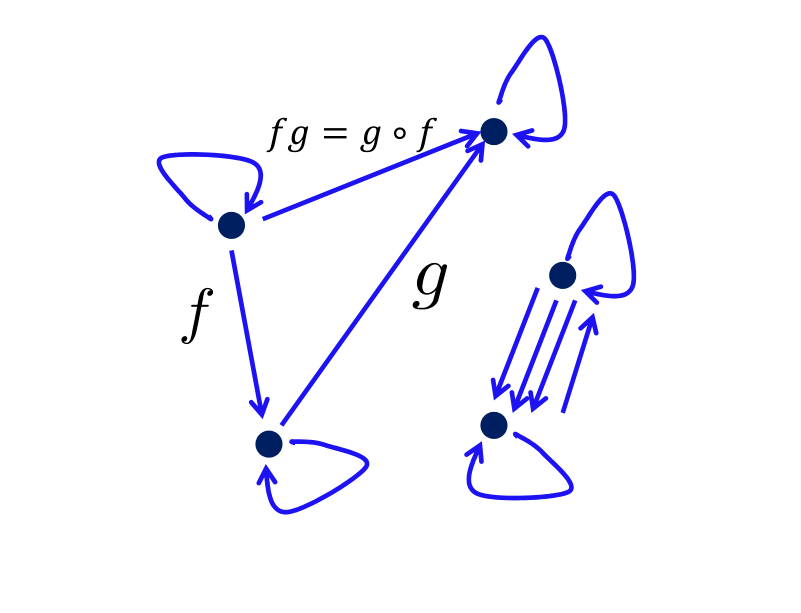
\includegraphics[width=0.55\textwidth]{figures/fig39.png}
  \caption{范畴的图示。对象是图中的黑点；图中画出了各条箭头，而人们必须给出一个规则，
    把每个箭头与别的箭头复合，并把复合的结果与某个箭头等同起来。例如，给定记作 $f$ 与 $g$
    的两个箭头，就必然存在一个形如 $f\circ g$ 的箭头。注意每个对象 $x$ 至少有一条箭头，
    即 $\operatorname{Hom}(x,x)$ 中的恒等箭头。（原文 Fig.~39，第 236 页）}
  \label{fig:39}
\end{figure}

为了看出这与我们先前关于群的概念是等价的，我们给每个态射配上一个群元素。态射的复合就是群的乘法，而态射的可逆性就是逆元素的存在性。

我们将简要描述这一观点所提供的、关于群的一个重要的、影响深远的推广。然后我们将说明，这一观点会导向一个漂亮的几何构造，它使群上同调（group cohomology）的公式变得稍微更直观一些。

\subsection{群胚} % 原文: K.1 Groupoids

\textbf{定义}\quad 一个\emph{群胚}（groupoid）是所有态射都可逆的范畴。

注意，对群胚中的任何对象 $x$，$\hom(x,x)$ 都是一个群，称为对象 $x$ 的\emph{自同构群}（automorphism group）。

\textbf{例 1}\quad 集合 $X$ 上的任何等价关系都定义一个群胚。其对象是 $X$ 的元素。若 $a\sim b$，则集合 $\hom(a,b)$ 恰有一个元素，否则为空集。态射的复合律于是意味着：$a\sim b$ 且 $b\sim c$ 蕴含 $a\sim c$。显然，每个态射都可逆。

% [Tutor Note: 「群胚」（groupoid）也有「广群」这一旧译，本译本统一用「群胚」，与 c27 一致。
% 定义处最易误读的一点是：群胚\emph{不是}群。$\hom(x,x)$ 只是对象 $x$ 的自同构群，不同对象之间的
% $\hom(x,y)$ 一般非空，故不能把整个群胚当成一个群来「乘」。例 3 正是这一区别的实例：
% 基本群胚 $\pi_{\le1}(X)$ 的对象是 $X$ 的\emph{所有}点，而基本群 $\pi_1(X,x)$ 只是其中某个
% $\hom(x,x)$；把两者混为一谈，就会误以为 $\pi_{\le1}(X)$ 依赖于基点的选取。]

\textbf{例 2}\quad 考虑量子力学中哈密顿量含时的时间演化。谈论演化算符 $U(t)$ 是没有意义的；人们必须谈论满足 $U(t_1,t_2)U(t_2,t_3)=U(t_1,t_3)$ 的酉演化 $U(t_1,t_2)$。给定 Schrödinger 方程的一个解 $\Psi(t)$，我们可以把态矢量 $\Psi(t)$ 视为对象，把 $U(t_1,t_2)$ 视为态射。这样，Schrödinger 方程的一个解就定义了一个群胚。

{\small\itshape ［原文标记：需要澄清这段话。］}
% [原文待办标记，原文 p.236 右侧页边注：\ensuremath{\clubsuit}Clarify this remark.\ensuremath{\clubsuit}]

\textbf{例 3}\quad 设 $X$ 是拓扑空间。基本群胚（fundamental groupoid）$\pi_{\le 1}(X)$ 是这样一个范畴：其对象是点 $x\in X$，其态射是道路 $f:x\to x'$ 的同伦类。这些态射按自然的方式复合。注意，点 $x\in X$ 的自同构群，即 $\hom(x,x)$，就是以 $x$ 为基点的 $X$ 的基本群 $\pi_1(X,x)$。

\textbf{例 4}\quad 规范场论：对象 = 主丛上的联络；态射 = 规范变换。对于理解超引力与弦论中出现的、由更高次微分形式构成的某些更奇特的（阿贝尔）规范场论来说，这是正确的观点。

\textbf{例 5}\quad 在弦论的轨道流形（orbifold）与 orientifold 理论中，时空必须被视为一个群胚。设 $G$ 右作用在集合 $X$ 上，于是有一个映射
\begin{equation}
  \Phi:X\times G\to X
  \tag{K.37}
  \label{eq:K.37}
\end{equation}
使得
\begin{equation}
  \Phi(\Phi(x,g_1),g_2)=\Phi(x,g_1g_2)
  \tag{K.38}
  \label{eq:K.38}
\end{equation}
\begin{equation}
  \Phi(x,1_G)=x
  \tag{K.39}
  \label{eq:K.39}
\end{equation}
对一切 $x\in X$ 与 $g_1,g_2\in G$ 成立。为简短起见，我们直接写 $\Phi(x,g):=x\cdot g$。于是可以构造范畴 $X/\!/G$，其中
\begin{equation}
\begin{split}
  \mathit{Ob}(X/\!/G) &= X\\
  \mathit{Mor}(X/\!/G) &= X\times G
\end{split}
\tag{K.40}
\label{eq:K.40}
\end{equation}
我们应当把态射想成一条以 $g$ 标记的箭头，把点 $x$ 连到点 $x\cdot g$。靶映射与源映射为
\begin{equation}
  p_0((x,g)):=x\cdot g \qquad p_1((x,g)):=x
  \tag{K.41}
  \label{eq:K.41}
\end{equation}

{\small\itshape ［原文标记：此处需要插图！］}
% [原文待办标记，原文 p.237 右侧页边注：\ensuremath{\clubsuit}FIGURE NEEDED HERE! \ensuremath{\clubsuit}]

态射的复合定义为
\begin{equation}
  (xg_1,g_2)\circ(x,g_1):=(x,g_1g_2)
  \tag{K.42}
  \label{eq:K.42}
\end{equation}
或者，用另一种记号（更适合右作用）：
\begin{equation}
  (x,g_1)(xg_1,g_2):=(x,g_1g_2)
  \tag{K.43}
  \label{eq:K.43}
\end{equation}
注意 $(x,1_G)\in\hom(x,x)$ 是恒等态射；而态射的复合之所以有意义，正是因为我们有一个群作用。还要注意，$\mathrm{pt}/\!/G$（其中 $G$ 平凡地作用在一个点上）把群 $G$ 实现为一个范畴，如上文所勾勒。

% [Tutor Note: (K.42) 与 (K.43) 是同一复合律的两种写法，但\emph{字的左右次序相反}：
% (K.42) 用熟悉的 $\circ$ 记号，(xg_1,g_2)\circ(x,g_1) 表示先走 $g_1$、再走 $g_2$，
% 即「$\circ$ 右边先作用」；(K.43) 改用并置，写成 (x,g_1)(xg_1,g_2)，把先作用的 $g_1$ 放在
% 左边。抄写或编程时若把两式的次序对齐错，会得到 $g_1g_2$ 与 $g_2g_1$ 互换的错误复合
% （对非阿贝尔 $G$，这不是小错）。核对办法：代入 $g_1=1_G$，两式都应退化为恒等态射。]

% 转写说明：例 5 与例 6 的首句在原文中逐字相同（原文 p.237），例 6 只剩这一句、
% 没有下文，显然是作者原稿中复制粘贴留下的残句。此处照录，不作合并；读者理解例 6 时
% 应把例 5 的全部内容（含 (K.37)--(K.43)）算作它的正文。

\textbf{例 6}\quad 在弦论的轨道流形与 orientifold 理论中，时空必须被视为一个群胚。（这与上一个例子密切相关。）

\medskip
\noindent\rule{\linewidth}{0.4pt}
\medskip
\noindent\textbf{练习}

设 $G$ 是一个群。我们定义一个群胚，记作 $G/\!/G$（理由见后文），其对象是群元素 $\mathit{Obj}(G/\!/G)=G$，其态射是由
\begin{equation}
  g_1\xrightarrow{\ h\ }g_2
  \tag{K.44}
  \label{eq:K.44}
\end{equation}
给出的箭头，即当且仅当 $g_2=h^{-1}g_1h$ 时才存在的箭头。这是圆周上主 $G$-丛的群胚。

画出对应于 $S_3$ 的群胚。

\subsection{张量范畴} % 原文: K.2 Tensor Categories

为了定义 TFT，我们需要张量范畴（tensor category）这一进一步的概念。注意，给定一个范畴 $C$，笛卡尔积 $C\times C$、$C\times C\times C$、…… 也按自然的方式成为范畴。

\textbf{定义}\quad 一个\emph{张量范畴}（tensor category，也称\emph{幺半范畴} monoidal category）是带有一个函子 $\otimes:C\times C\to C$ 的范畴，使得两个函子 $\otimes\circ\otimes_{12}:C\times C\times C\to C$ 与 $\otimes\circ\otimes_{23}:C\times C\times C\to C$ 之间存在一个同构 $\mathcal{A}$ 满足五边形公理（pentagon identity），并且存在一个单位对象（identity object）$1_C$，连同函子 $C\to C$ 之间的自然变换
\begin{equation}
  \iota_L:1_C\otimes\cdot\ \to\mathrm{Id}
  \tag{K.45}
  \label{eq:K.45}
\end{equation}
\begin{equation}
  \iota_R:\cdot\otimes 1_C\to\mathrm{Id}
  \tag{K.46}
  \label{eq:K.46}
\end{equation}
这些数据还需服从若干自然的相容性条件：

{\small\itshape ［原文标记：我们是否要求对偶对象存在？］}
% [原文待办标记，原文 p.238 右侧页边注：\ensuremath{\clubsuit}Do we require the existence of a dual object?\ensuremath{\clubsuit}]

为举例说明这些相容性条件，我们考虑关于自然变换 $\mathcal{A}$ 的第一个条件：对 $C_0$ 中的一切对象 $x,x',x''$，有一个同构
\begin{equation}
  \mathcal{A}_{x,x',x''}:(x\otimes x')\otimes x''\to x\otimes(x'\otimes x'')
  \tag{K.47}
  \label{eq:K.47}
\end{equation}
它满足五边形公理：

% 转写说明：主文件未载入绘图宏包，故五边形交换图用 array 排布；五个顶点、五条箭头的
% 方向与原文 p.238 的图一致（上行的水平箭头、两侧的斜箭头，以及底部汇合的斜箭头）。

{\small
\begin{equation}
\begin{array}{ccc}
\big((x_1\otimes x_2)\otimes x_3\big)\otimes x_4 & \longrightarrow &
\big(x_1\otimes x_2\big)\otimes\big(x_3\otimes x_4\big)\\[10pt]
\swarrow & & \searrow\\[10pt]
\big(x_1\otimes(x_2\otimes x_3)\big)\otimes x_4 & &
x_1\otimes\big(x_2\otimes(x_3\otimes x_4)\big)\\[10pt]
\searrow & & \nearrow\\[10pt]
& x_1\otimes\big((x_2\otimes x_3)\otimes x_4\big) &
\end{array}
\tag{K.48}
\label{eq:K.48}
\end{equation}
}

{\small\itshape ［原文标记：修正 $xy$ 矩阵。］}
% [原文待办标记，原文 p.238 右侧页边注：\ensuremath{\clubsuit}FIX xy matrix \ensuremath{\clubsuit}，紧挨着上面的五边形图；
% 所指应是图中 $x_1,\dots,x_4$ 的下标排布（或图中箭头的 $x,y$ 记号），原意不明，照录。]

于是有定理（“相干定理”，coherence theorem）：无论怎样加括号，$x_0\otimes x_1\otimes\cdots\otimes x_n$ 在相差同构的意义下都是良定义的。关于自然变换 $\iota_L$ 与 $\iota_R$ 的条件则相当显然。

\textbf{例}\quad 范畴 $\mathbf{VECT}_\kappa$ 是张量范畴。张量单位 $1_{\mathbf{VECT}_\kappa}$ 是什么？

设 $\sigma:C\times C\to C\times C$ 是交换函子（exchange functor），它在对象与态射上交换两个因子。

\textbf{定义}\quad 一个\emph{对称幺半范畴}（symmetric monoidal category）是带有一个同构 $\Omega$ 的幺半范畴，该 $\Omega$ 是 $\otimes\circ\sigma$ 与 $\otimes$ 之间的同构，且其平方为恒等。同样，它与 $\mathcal{A}$、$\iota_L$、$\iota_R$ 之间有许多相当显然的相容性条件。

这仍然意味着，对一切对象 $x,y$ 都有同构
\begin{equation}
  \Omega_{x,y}:x\otimes y\to y\otimes x
  \tag{K.49}
  \label{eq:K.49}
\end{equation}
使得 $\Omega_{y,x}\circ\Omega_{x,y}=1_{x\otimes y}$。

% [Tutor Note: 定义里要求的是「自然变换」$\iota_L,\iota_R$，而 (K.45)(K.46) 又额外说它们
% 是「同构」——两件事不能混：自然变换只需要每个分量 $(\iota_L)_x:1_C\otimes x\to x$ 存在并与
% 态射相容，而同构还要求每个分量可逆。张量范畴的公理必须\emph{同时}给出结合子 $\mathcal{A}$
% (K.47) 与左右单位子 (K.45)(K.46)；相干定理的作用正是保证只需验证五边形公理 (K.48) 与
% 三角形公理，而不必逐一验证「任意加括号方式的复合都相等」这无穷多条等式。作者的
% "fairly obvious" 指的就是三角形公理那一条，原文未写出，读者可自行补出：
% $(x\otimes 1_C)\otimes y\xrightarrow{\ \mathcal{A}\ }x\otimes(1_C\otimes y)
% \xrightarrow{\ 1\otimes\iota_L\ }x\otimes y$ 应等于 $\iota_R\otimes 1$。
% 术语取舍：原文在定义张量范畴时明说 "also known as a monoidal category"，
% 即把 tensor category 与 monoidal category 当作同义词；但严格说这是两个层次——monoidal
% 只要求 (K.45)--(K.48) 这一套（结合子、单位子、五边形、三角形），symmetric 则是在此之上
% 再加一个平方为 $1$ 的 $\Omega$ (K.49)。本译本按原文把前者译「张量范畴/幺半范畴」、
% 后者译「对称幺半范畴」；读文献时若见到 "tensor category" 指「带刚性（对偶）的对称
% 幺半范畴」（如 Deligne--Milne 的用法），要按上下文判断，不能一律套用本节定义。
% 紧接着引入的 braided（编织）是本书反复用到的概念（任意子的编织），务必与 symmetric 区分：
% 编织只要求 $\Omega$ 可逆，\emph{不}要求 $\Omega^2=1$；$\Omega^2=1$ 的编织范畴正是对称
% 幺半范畴。$2+1$ 维任意子的统计相位一般不为 $\pm1$，所以物理上真正需要的是编织而非对称
% ——这正是作者在此处把它作为「重要推广」引入的原因。]

\textbf{注}\quad 对共形场论以及 $2+1$ 维中的准粒子统计而言，一个重要推广是\emph{编织张量范畴}（braided tensor category）的概念：其中仍有同构 $\Omega$，但它的平方不为 $1$。

最后，我们需要（对称）张量函子（tensor functor）这一记号。它是两个对称张量范畴之间的函子 $F:C\to D$，连同同构 $1_D\to F(1_C)$，以及两个函子 $C\times C\to D$（分别由 $F\circ\otimes$ 与 $\otimes\circ F\times F$ 给出）之间的一个同构。

\subsubsection{$\mathbb{Z}_2$ 分次向量空间} % 原文: K.2.1 Z2-graded vector spaces

一个 $\mathbb{Z}_2$ 分次向量空间是带有分解 $V=V_0\oplus V_1$ 的向量空间，其中下标被理解为 $\mathbb{Z}_2$ 的元素。在 $\mathbb{Z}_2$ 分次向量空间的范畴中，我们可以引入两种不同的张量范畴。对于 $\mathbb{Z}_2$ 分次向量空间，我们能够并且将会使用分次张量积（graded tensor product）。此时有同构
\begin{equation}
  \Omega:V\otimes W\to W\otimes V
  \tag{K.50}
  \label{eq:K.50}
\end{equation}
但必须小心地运用 Koszul 符号规则：若 $v,w$ 是齐次元素，则
\begin{equation}
  \Omega(v\otimes w)=(-1)^{|v|\cdot|w|}\,w\otimes v
  \tag{K.51}
  \label{eq:K.51}
\end{equation}
这条规则有一个重要推论：如果我们有任何一族超向量空间（supervector space）$(V_\alpha)_{\alpha\in I}$（其中下标 $\alpha$ 标记不同的超向量空间，不应与 $\mathbb{Z}_2$ 分次混淆），那么就存在唯一一个典范的张量积
\begin{equation*}
  \bigotimes_{\alpha}V_\alpha
\end{equation*}
而无需指定任何次序。

% [Tutor Note: (K.51) 的符号因子指数是 $|v|\cdot|w|$，其中 $|v|,|w|\in\{0,1\}$ 是
% $\mathbb{Z}_2$ 次数（\emph{不是} $\mathbb{Z}$-次数，也不是 $V$ 的维数）。两个奇元素交换
% 两次给出 $(-1)^{1\cdot1}\cdot(-1)^{1\cdot1}=+1$，故交换子平方为恒等；而两个奇元素之间的
% 一次交换给出 $-1$（交换两次才回到原状），这正是「典范张量积无需指定次序」的来源：换序
% 至多差一个由次数决定的符号，而这个符号不依赖于换序的路径。抄写时最易把
% $(-1)^{|v||w|}$ 写成 $(-1)^{|v|+|w|}$，后者对两个奇元素给出 $+1$，与超代数约定相反。]

\subsubsection{群的表示范畴} % 原文: K.2.2 Category Of Representations Of A Group

设 $G$ 是一个群。那么存在一个范畴，其对象是表示，态射是表示之间的缠结算子（intertwiner），即与 $G$ 的作用交换的表示之间的映射。

现在设 $G$ 是紧群，并限制到有限维表示的子范畴。记之为 $\mathrm{Rep}(G)$。这是一个张量范畴。此外，有一组“单”对象，即不可约表示 $V_\lambda$，使得所有对象都同构于单对象的直和。张量函子由“融合规则”（fusion rules）
\begin{equation}
  V_\lambda\otimes V_\mu\cong D^\rho_{\lambda\mu}\otimes V_\rho
  \tag{K.52}
  \label{eq:K.52}
\end{equation}
决定，其中 $D^\rho_{\lambda\mu}$ 是描述简并的有限维实向量空间。

% [Tutor Note: (K.52) 照原文转写，但它用的是对 $\rho$ 的隐式求和并省略了直和号；
% 通常的写法是 $V_\lambda\otimes V_\mu\cong\bigoplus_\rho D^\rho_{\lambda\mu}\otimes V_\rho$，
% 其中 $D^\rho_{\lambda\mu}$ 是多重数空间，$\dim D^\rho_{\lambda\mu}=N^\rho_{\lambda\mu}$
% 即融合系数（非负整数）。若把 (K.52) 当等式逐项读而不求和，就会得出「两个不可约表示的
% 张量积仍是不可约的」这一错误结论——只有 $G=U(1)$ 这类情形才对。]

\section{配边} % 原文: L. Bordism

\begin{keytakeaways}
  \item 配边的定义 \eqref{eq:L.1}：从闭 $(d-1)$ 维流形 $Y_0$ 到 $Y_1$ 的配边是一个 $d$ 维流形 $X$，
    其边界被不交地划分为 $(\partial X)_0\sqcup(\partial X)_1$，并带有从边界「领」（collar）
    $[0,1)\times Y_0$、$(-1,0]\times Y_1$ 到 $X$ 的嵌入 $\theta_0,\theta_1$；这些额外数据的作用
    正是使粘合（gluing）有定义。
  \item 群结构：不交并给出 $n$ 维流形配边等价类 $\Omega_n$ 上的阿贝尔群结构，空集 $\varnothing^n$
    是零元；$[0,1]\times X$ 给出 $X\sqcup X$ 与 $\varnothing$ 的配边，故 $2[X]=0$，每个元素都是二阶的。
  \item 低维计算：$\Omega_0\cong\mathbb{Z}/2\mathbb{Z}$（两个点零配边）、$\Omega_1=0$（圆周是圆盘的边界）、
    $\Omega_2\cong\mathbb{Z}/2\mathbb{Z}$（生成元 $[\mathbb{RP}^2]$，用 Euler 示性数的奇偶性论证）。
  \item Thom 定理 \eqref{eq:L.2}：$\Omega_*\cong R[x_2,x_4,x_5,\dots]$，$R=\mathbb{Z}/2\mathbb{Z}$，
    $k$ 次生成元 $x_k$ 恰有一个，且只对 $k\ne 2^j-1$ 出现；偶次生成元是 $\mathbb{RP}^k$ 的配边类。
  \item 范畴化：$\mathrm{Bord}_{\langle d-1,d\rangle}$ 以闭 $(d-1)$ 维流形为对象、配边的同胚类为态射，
    复合是粘合，它是对称张量范畴（不交并为张量积、空流形为单位）；有向版本见第 L.3 小节，
    它要求边界嵌入保定向，并给出对偶配边 $X^\vee:Y_1^\vee\to Y_0^\vee$。
\end{keytakeaways}

这一数学主题是拓扑场论的重要背景。关于该主题有一本经典著作：
\begin{quote}
Milnor and Stasheff, \emph{Characteristic Classes}, PUP\\
更技术性的细节可在 R. Stong 的书中找到。\\
此外，我们还使用了 Dan Freed 那份非常好的讲义中的一些材料：\\
D. Freed, ``Bordism Old And New,''\\
\url{https://www.ma.utexas.edu/users/dafr/M392C-2012/index.html}
\end{quote}

\subsection{无向配边：定义与例子} % 原文: L.1 Unoriented Bordism: Definition And Examples

下面给出配边（bordism）的正式定义：

\textbf{定义}\quad 设 $Y_0,Y_1$ 是两个闭的 $(d-1)$ 维流形。从 $Y_0$ 到 $Y_1$ 的一个\emph{配边}是
\begin{enumerate}
  \item 一个 $d$ 维流形 $X$，连同其边界的一个不交划分
  \begin{equation}
    \partial X=(\partial X)_0\sqcup(\partial X)_1
    \tag{L.1}
    \label{eq:L.1}
  \end{equation}
  \item 一对嵌入 $\theta_0:[0,1)\times Y_0\to X$ 与 $\theta_1:(-1,0]\times Y_1\to X$，它们是到其像上的微分同胚，并且使得限制 $\theta_0:\{0\}\times Y_0\to(\partial X)_{\mathrm{in}}$ 与 $\theta_1:\{0\}\times Y_1\to(\partial X)_{\mathrm{out}}$ 都是同胚。
\end{enumerate}

与我们先前所说的相比，这个定义之所以多出一层复杂性，是因为这些额外的数据便于把配边粘合起来产生新的配边。

容易看出，配边是一个等价关系；而不交并（disjoint union）在 $n$ 维流形的配边等价类空间 $\Omega_n$ 上定义一个阿贝尔群结构。该群的零元素是空集 $\varnothing^n$ 的等价类；任何闭 $n$ 维流形 $X$ 都是自己的逆元，因为 $[0,1]\times X$ 可以看作 $X\sqcup X$ 与 $\varnothing$ 之间的一个配边。于是在 $\Omega_n$ 中 $2[X]=0$。

\textbf{例}

\begin{enumerate}
  \item 只有一种非平凡的零维流形，即点；而我们刚刚看到，两个点的不交并是零配边的，因此 $\Omega_0\cong\mathbb{Z}/2\mathbb{Z}$。注意，若去掉对 $X$ 的流形条件，那么字母 Y（即 Y 形的空间）就会给出两个点（等价于零）与一个点之间的一个配边，于是配边群将是平凡的。因此，流形条件是重要的。
  \item $\Omega_1=0$，因为唯一的闭连通一维流形是圆周，而它显然是一个圆盘的边界。
  \item 可以证明 $\Omega_2\cong\mathbb{Z}/2\mathbb{Z}$，生成元是 $[\mathbb{RP}^2]$。其论证如下（取自 D. Freed 的讲义 ``Bordism Old And New,'' 见其主页）。紧曲面的分类表明，曲面由两个不变量刻画：可定向性与 Euler 示性数。可定向曲面显然零配边。请注意！Euler 示性数\emph{不是}配边不变量！不可定向曲面都可由与 $\mathbb{RP}^2$ 作连通和得到。两个 $\mathbb{RP}^2$ 的连通和是圆周上的圆丛。取 $[0,1]\times S^1$ 并按 $\{(0,z)\}\sim\{(1,\bar z)\}$ 作商（其中把 $S^1$ 视为单位复数）。注意，我们可以把 $S^1$ 换成圆盘 $D^2$，并用同样的等同 $\{(0,z)\}\sim\{(1,\bar z)\}$ 得到从 Klein 瓶到零的一个配边。下面我们断言，$\mathbb{RP}^2$ 给出一个非平凡的配边类。因为，若它有一个到零的配边、即 $\partial X=\mathbb{RP}^2$，则对 $X$ 作三角剖分就给出双倍 $X\cup_{\mathbb{RP}^2}X$ 的一个三角剖分，其 Euler 示性数为 $2\chi(X)-1$。另一方面，闭三维流形的 Euler 示性数为零。现在，一般的连通不可定向曲面是 $n$ 个 $\mathbb{RP}^2$ 的连通和。把它们两两分组，并为每一对取一个到零的配边，就可以把配边类等同于 $\mathbb{Z}/2\mathbb{Z}$ 中的元素 $n\bmod 2$。
  \item 为描述全部配边群 $\Omega_d$，有用的一点是注意到流形的笛卡尔积与配边等价关系相容，这使得 $\Omega_*\cong\bigsqcup_{d\ge 0}\Omega_d$ 成为一个 $\mathbb{Z}$-分次环，分次由维数给出。Thom 证明了
  \begin{equation}
    \Omega_*\cong R[x_2,x_4,x_5,x_6,x_8,x_9,x_{10},x_{11},x_{12},x_{13},x_{14},x_{16},x_{17},\dots]
    \tag{L.2}
    \label{eq:L.2}
  \end{equation}
  其中 $R=\mathbb{Z}/2\mathbb{Z}$，并且只要 $k$ 不是 $2^j-1$ 的形式，就恰有一个 $k$ 次生成元 $x_k$。偶次生成元是 $\mathbb{RP}^k$ 的配边类，奇次生成元则是 $(S^m\times\mathbb{CP}^\ell)/\mathbb{Z}_2$ 的一个商，其中 $\mathbb{Z}_2$ 的作用是（对径映射，复共轭）。
  \item 此外，对任何流形都有一系列上同调类 $w_i(Y)\in H^i(Y;\mathbb{Z}/2\mathbb{Z})$，称为 Stiefel-Whitney 类。它们与切丛的扭曲（twisting）相关联。（例如，$w_1(Y)$ 刻画 $Y$ 是否可定向。）一个流形的\emph{Stiefel 数}是 $\mathbb{Z}/2\mathbb{Z}$ 中元素构成的序列
  \begin{equation}
    \langle w_{i_1}(Y)\cup\cdots\cup w_{i_k}(Y),[Y]\rangle
    \tag{L.3}
    \label{eq:L.3}
  \end{equation}
  而两个流形配边，当且仅当它们的全部 Stiefel 数都相同。关于最后两项，参见 Milnor 与 Stasheff 的优秀著作 \emph{Characteristic Classes}。\footnote{如果我们讲到特征类那一章，就会证明这两个结果。}
\end{enumerate}

% [Tutor Note: 第 3 条从「$X\cup_{\mathbb{RP}^2}X$ 的 Euler 示性数为 $2\chi(X)-1$」到矛盾，
% 缺了一步：双倍公式应为 $\chi(\text{double})=2\chi(X)-\chi(\mathbb{RP}^2)$，而
% $\chi(\mathbb{RP}^2)=1$，故该数为奇数；闭三维流形的 Euler 示性数为 $0$（偶数），矛盾。
% 作者省略了「$\chi(\mathbb{RP}^2)=1$」与「奇数不等于零」这两小步。另注意本段用的
% Euler 示性数对带边流形也成立（拓扑不变量），无需可定向性，这正是论证能用于不可定向曲面的原因。]

\subsection{配边范畴 $\mathrm{Bord}_{\langle d-1,d\rangle}$} % 原文: L.2 The Bordism Category Bord$\langle d-1,d\rangle$

现在我们可以定义一个\emph{配边范畴} $\mathrm{Bord}_{\langle d-1,d\rangle}$。
\begin{enumerate}
  \item 对象：闭的 $(d-1)$ 维流形，通常记作 $Y$。
  \item $\hom(Y_0,Y_1)$ 是配边 $X:Y_0\to Y_1$ 的同胚类的集合。配边 $X$ 与 $X'$ 之间的一个同胚，是带边流形之间的同胚，它把 $(\partial X)_{\mathrm{in}}$ 送到 $(\partial X')_{\mathrm{in}}$，并与领 $\theta_0,\theta_1$ 交换。
\end{enumerate}

配边范畴中态射的复合通过粘合实现。由于我们按同胚来等同配边，配边 $X=[0,1]\times Y$（从 $Y$ 到 $Y$）就是恒等态射 $1_Y$。范畴 $\mathrm{Bord}_{\langle d-1,d\rangle}$ 是一个对称张量范畴：张量积是不交并，而空流形 $\varnothing^{d-1}$ 是张量单位。

% [Tutor Note: 范畴约定：这里的态射是配边的\emph{同胚类}，不是微分同胚类——无向配边
% 范畴根本不带光滑结构，「微分同胚」无从谈起；到了有向情形 (L.3)，才改用保定向的
% \emph{微分同胚}来等同。两处若混用，粘合的定义与恒等态射 $1_Y=[0,1]\times Y$ 的验证都会
% 出问题（例如 $[0,1]\times Y$ 与 $[0,2]\times Y$ 只在同胚意义下相同，而非微分同胚意义下
% 逐点相同）。另外注意「领」（collar）$\theta_0,\theta_1$ 是态射数据的一部分：没有它，
% 粘合只能定义到同胚为止，复合的结合律无法直接验证。]

\subsection{有向配边范畴 $\mathrm{Bord}^{\mathrm{SO}}_{\langle d-1,d\rangle}$} % 原文: L.3 The Oriented Bordism Category Bord$^{SO}_{\langle d-1,d\rangle}$

我们常常关心\emph{有向配边}（oriented bordism）。

为了定义有向配边，我们对配边的定义略作修改。现在 $Y_0,Y_1,X$ 都是定向的。嵌入 $\theta_0$ 与 $\theta_1$ 要求保持定向，并且我们按定向微分同胚来等同配边 $X$ 与 $X'$。

$\theta_0$ 与 $\theta_1$ 保持定向这一条件必须小心处理。注意，如果给定若干定向实向量空间的一个和，那么直和上并没有自然的定向。然而，如果给定一个正合序列
\begin{equation}
  0\to V_1\to V_2\to V_3\to 0
  \tag{L.4}
  \label{eq:L.4}
\end{equation}
那么就有一个典范同构 $\operatorname{DET}V_3\cong\operatorname{DET}V_1\to\operatorname{DET}V_2$；因此，若三个空间中有两个已定向，我们便可要求这个典范同构保持定向，从而确定第三个空间的定向。特别地，子流形与外围流形上的定向确定了法丛上的定向。在定义 $\theta_0$、$\theta_1$ 时，我们用 $\mathbb{R}$ 上的标准定向 $+\partial/\partial x$ 来定向 $[0,+1)$ 与 $(-1,0]$，然后取 $[0,+1)\times Y$ 与 $(-1,0]\times Y$ 上的乘积定向。

% [Tutor Note: 原文 (L.4) 之后印作 $\operatorname{DET}V_3\cong\operatorname{DET}V_1\to
% \operatorname{DET}V_2$，箭头处应是 $\otimes$：正合序列 $0\to V_1\to V_2\to V_3\to0$ 给出
% 行列式线丛的乘法性 $\operatorname{DET}V_2\cong\operatorname{DET}V_1\otimes
% \operatorname{DET}V_3$（等价地 $\operatorname{DET}V_3\cong\operatorname{DET}V_1\otimes
% \operatorname{DET}V_2$，取决于 $\operatorname{DET}$ 与对偶的约定）。这是原文 p.242 的
% 排印错误（$\otimes$ 误作 $\to$），译文照录未改；核对时可验一下维数：若 $V_3=V_2/V_1$，
% 则 $\dim V_2=\dim V_1+\dim V_3$，两边行列式线丛的次数相加才对得上。]

\textbf{定义}\quad 对每个有向配边 $X:Y_0\to Y_1$，都有一个\emph{对偶有向配边} $X^\vee:Y_1^\vee\to Y_0^\vee$。让我们仔细把它写出来，因为这容易引起混淆。$Y^\vee$ 表示带相反定向的 $Y$。$X^\vee$ 是取\emph{相同}定向的流形 $X$；但我们交换入边与出边。此外，
\begin{equation}
  \theta_0^\vee(t,y_1)=\theta_1(-t,y_1) \qquad \forall t\in[0,+1)\quad\&\quad y_1\in Y_1
  \tag{L.5}
  \label{eq:L.5}
\end{equation}
\begin{equation}
  \theta_1^\vee(t,y_0)=\theta_0(-t,y_0) \qquad \forall t\in(-1,0]\quad\&\quad y_0\in Y_0
  \tag{L.6}
  \label{eq:L.6}
\end{equation}
注意，$\theta_0^\vee$ 与 $\theta_1$ 之间的关系涉及一个反转定向的变换 $t\to -t$；因此，由于 $X^\vee$ 与 $X$ 具有相同的定向，我们要求 $Y$ 上的定向也反转。若忘掉定向，我们也得到无向情形下对偶配边的概念。

再一次地，我们可以定义有向配边群 $\Omega_n^{\mathrm{SO}}$（$n\ge 0$）、有向配边环 $\Omega_*^{\mathrm{SO}}$，以及有向配边范畴 $\mathrm{Bord}^{\mathrm{SO}}_{\langle d-1,d\rangle}$。

\textbf{例 1}\quad 考虑有向配边群 $\Omega_0^{\mathrm{SO}}$。点有两种：$\mathrm{pt}_+$ 与 $\mathrm{pt}_-$；基本连通有向配边有五种，如图 40 所示。于是 $\Omega_0^{\mathrm{SO}}\cong\mathbb{Z}$。该同构取 $+$ 点数目与 $-$ 点数目的差。

\textbf{例 2}\quad 在 $1$ 维与 $2$ 维，我们同样得到零配边群。

% =====================================================================
%  c29 —— 原文印刷页 243--244（PDF 第 244--245 页）
%  含：L.3 末尾（图 40 与有向配边环的结构定理）、L.4 其他配边范畴、
%      M. 课程笔记中的若干来源、致谢（Acknowledgements）
%  编号公式：L.7、L.8；插图：Fig. 40。
%  注：印刷页 244 下半页起为 References（[1]--[72]），按分工由 chunks/c-refs.tex
%      处理，本片段到「References」标题之前为止，不转写任何文献条目。
%  全部内容逐页对照 150 dpi 页面图像（p244.png、p245.png）核校。
% =====================================================================

\begin{figure}[htbp]
  \centering
  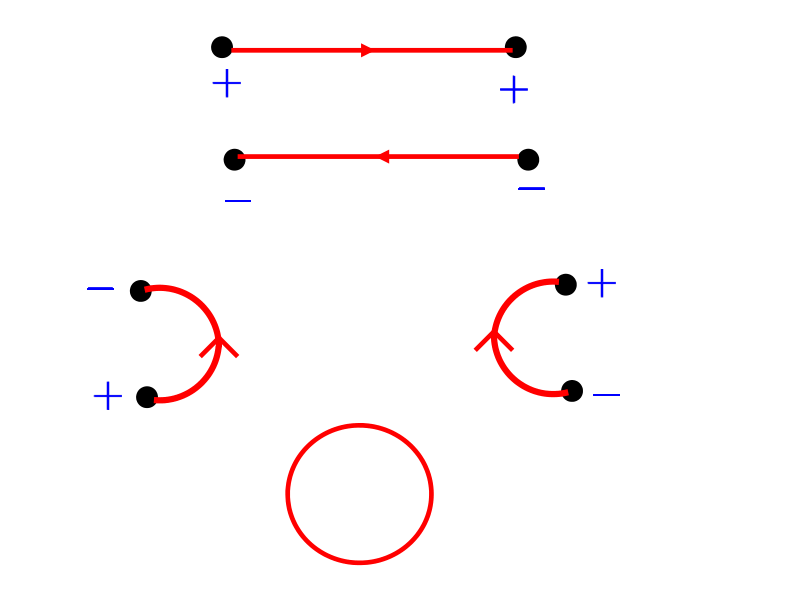
\includegraphics[width=0.55\textwidth]{figures/fig40.png}
  \caption{有向配边范畴中的五个连通配边。入边界在左，出边界在右。（原文 Fig.~40，第 243 页）}
  \label{fig:40}
\end{figure}

关于有向配边环 $\Omega_*^{SO}$ 的主要因子，总结如下。（见 Milnor 与 Stasheff。Freed 的讲义中在定理 2.24 附近还给出了若干进一步的文献。）\footnote{若我们讲到特征类那一章，就会证明其中一些结果。}

% 转写说明：原文此处只印有粗体的「Theorem」，并无编号；此处沿用主文件预定义的
% theorem 环境（与 c23 中同类情形一致），编号由 LaTeX 自动生成。

\begin{theorem}
\normalfont % 原文定理正文为直立体；中文无真正的斜体，故置正体（数学模式不受影响）
\begin{enumerate}
  \item $\Omega_*^{SO}$ 中所有挠元（torsion element）的阶都是二。
  \item $\Omega_*^{SO}/\,\mathrm{torsion}$ 是一个环，它在每个次数 $4k$（$k\ge 1$）上恰有一个生成元。
  \item 存在同构
  \begin{equation}
    \Omega_*^{SO}\otimes\mathbb{Q} \cong \mathbb{Q}[y_4,y_8,\cdots]
    \tag{L.7}
    \label{eq:L.7}
  \end{equation}
  在此同构下，$y_{4k}$ 对应于 $\mathbb{CP}^{2k}$ 的有向配边类。
  \item $Y$ 的切丛有特征类，即 Stiefel-Whitney 类 $w_i(Y)\in H^i(Y;\mathbb{Z}_2)$ 与 Pontryagin 类 $p_i(Y)\in H^{4i}(Y;\mathbb{Z})$（后者依赖于 $Y$ 的定向），使得 $Y_1$ 与 $Y_2$ 配边当且仅当所有 Stiefel-Whitney 数与 Pontryagin 数都相同。我们上文已定义了 Stiefel-Whitney 类，而 Pontryagin 数同样是如下这一族数
  \begin{equation}
    \langle p_{i_1}(Y)\cup\cdots\cup p_{i_k}(Y),[Y]\rangle \in \mathbb{Z}
    \tag{L.8}
    \label{eq:L.8}
  \end{equation}
\end{enumerate}
\end{theorem}

% [Tutor Note: 作者所说的「主要因子」(main factors) 指环 $\Omega_*^{SO}$ 的乘性生成元
% （即环论意义下的「素因子」），不是「主要因素」；译作「主要因子」只为与原文用词对应。
% 第 2 条与第 3 条须合读：第 2 条给出无挠部分在每个次数 $4k$ 上一个生成元，第 3 条则说明
% 张量 $\mathbb{Q}$ 后挠元消失（正是第 1 条「阶为二」的直接后果：阶为二的元素在
% $\mathbb{Q}$-系数下变成零），剩下的多项式环由 $y_{4k}\leftrightarrow[\mathbb{CP}^{2k}]$
% 生成。核对次数时注意 $\mathbb{CP}^{2k}$ 的\emph{实}维数是 $4k$，所以生成元次数为
% $4,8,12,\dots$ 即 $4k$，不是 $2k$；若误记为 $2k$，(L.7) 右端的下标就要全部改成
% $y_2,y_4,\dots$，而这与 (L.8) 中 Pontryagin 类所在次数 $4i$ 无法配对。]

% [Tutor Note: 定理第 4 条原文印作「such that $Y_1$ and $Y_2$ and bordant iff …」，
% 第二个 and 显然是 are 的笔误（应为「$Y_1$ and $Y_2$ are bordant iff …」），中文无法保留
% 这处拼写错误，故按文意译作「$Y_1$ 与 $Y_2$ 配边当且仅当……」。读这条判据时还须注意两件事：
% 其一，「所有 Stiefel-Whitney 数与 Pontryagin 数都相同」里的「所有」是指对一切可行多重指标
% $i_1\le\cdots\le i_k$ 取遍，而不是只取一个数；其二，(L.8) 的配对要求 $\dim Y=4(i_1+\cdots+i_k)$，
% 故奇数维流形的 Pontryagin 数全为零，那条判据在奇数维就退化为只看 Stiefel-Whitney 数——
% 这是 Thom 配边定理的标准形式，作者在此只是复述，未给证明（证明要用到 Thom 谱与
% Serre 关于稳定同伦群有限性的结果）。]

\subsection{其他配边范畴} % 原文: L.4 Other Bordism Categories

% 转写说明：原文此行写作「We can go on an consider other forms of bordism:」，
% 其中「an」应为「and」（笔误），译文按文意译出，未保留该拼写错误。

我们还可以接着考虑其他形式的配边：
\begin{enumerate}
  \item 标架配边（framed bordism）。（通过 Pontryagin-Thom 构造，它与球面的稳定同伦密切相关。）
  \item Spin 配边与 Pin$^{\pm}$ 配边。
  \item Riemann 配边（Riemannian bordism）。
\end{enumerate}

相应地，配边范畴也有各种推广。一般地，若我们计入某种结构 $\mathcal{S}$，就把配边范畴记作 $\mathrm{Bord}^{\mathcal{S}}_{\langle d-1,d\rangle}$；这里约定的意思是，配边之间用保持结构 $\mathcal{S}$ 的同胚来等同。于是，有向配边范畴记作 $\mathrm{Bord}^{SO}_{\langle d-1,d\rangle}$（因为切丛的结构群分别是 $SO(d-1)$ 与 $SO(d)$）。类似地我们可以定义 Riemann 配边范畴 $\mathrm{Bord}^{\mathrm{Riem}}_{\langle d-1,d\rangle}$，如此等等。

% [Tutor Note: 记号里上标与下标分工不同，最易写反：上标 $\mathcal{S}$ 是「所附加的结构」
% （定向、Spin、标架、Riemann 度规……），下标 $\langle d-1,d\rangle$ 是「维度档」——对象是
% $(d-1)$ 维闭流形、态射是 $d$ 维配边，与第 5 章的 $\mathrm{Bord}^{S}_{\langle d-1,d\rangle}$
% 完全同一套约定；这里用的是尖括号 $\langle\cdot,\cdot\rangle$，不要写成圆括号。
% 另一处易错点是括号里的结构群：$d$ 维配边的切丛结构群是 $SO(d)$，而其 $(d-1)$ 维边界上
% 因为有指向外（或内）的法向，结构群约化为 $SO(d-1)$，所以原文才说「分别是 $SO(d-1)$ 与
% $SO(d)$」；若在边界上也写 $SO(d)$，边界就带上了法向的冗余信息，配边的粘接不会自洽。
% 术语上 bordism 与 cobordism 在中译里都作「配边」，故本片段统一用「配边」，不加区分。]

\section{课程笔记中的若干来源} % 原文: M. Some Sources From Course Notes

\begin{keytakeaways}
  \item 本节不是论证，而是一份按主题分组的「素材出处」清单：作者把自己历年课程笔记中
    与正文各章配套的部分逐条列出，供读者按主题回溯原始材料。
  \item theta 函数与 Heisenberg 代数的材料见 GMP7-06 第 6 节与
    GMP-Ch8-AssociatedBundles-2010 第 11 节；这正是附录 D、E 中模变换律与环面上全纯线丛
    那套内容的上游笔记。
  \item 第 $k$ 级 theta 函数的\emph{不变范数}与第一 Chern 类见 GMP9-06 第 3.3 节——它对应
    正文中用 theta 函数构造预量子线丛的 Hermitian 结构那一步。
  \item 群上同调与 Dijkgraaf-Witten 理论见 GRP-THEORY-Lect1；拓扑场论与范畴见 GMP 2015。
    这两条分别接续正文关于有限群规范理论与扩展拓扑场论／张量范畴的讨论。
  \item 这些编号（GMP7-06、GMP9-06、GMP-Ch8-AssociatedBundles-2010、GRP-THEORY-Lect1、
    GMP 2015）是作者个人课程笔记的内部编号，不是正式发表的文献条目，因此与下文参考文献表
    互补而不重复。
\end{keytakeaways}

关于 theta 函数与 Heisenberg 代数的材料：
\begin{itemize}[label={},leftmargin=2.6em,itemsep=2pt,topsep=2pt]
  \item GMP7-06, section 6
  \item GMP-Ch8-AssociatedBundles-2010, section 11.
\end{itemize}

第 $k$ 级 theta 函数的不变范数（invariant norm）、第一 Chern 类：GMP9-06, section 3.3.

还有群上同调。一些 Dijkgraaf-Witten 理论。GRP-THEORY-Lect1

拓扑场论与范畴：GMP 2015.

% [Tutor Note: 这一节的行文是笔记索引而非普通段落，其中的「GMP7-06」「GMP-Ch8-
% AssociatedBundles-2010」「GMP9-06」「GRP-THEORY-Lect1」「GMP 2015」都是作者课程笔记的
% 文件名式编号，「section 6」「section 11」「section 3.3」是这些笔记内部的节号。译文照原样
% 保留这些拉丁字符串、未译成「第 6 节」，因为一旦译出就无法再与笔记原件对应；缩进的两行
% 是被「关于 theta 函数与 Heisenberg 代数的材料：」统领的子项，故用无标号列表复刻其缩进，
% 其余各行原文即为顶格，故仍作独立段落。原文各行的句末标点本就不统一（有的有句点、有的
% 没有），译文一仍其旧。]

\subsection*{致谢} % 原文: Acknowledgements

GM 谨向 2019 年 TASI 暑期学校的组织者致谢，感谢他们邀请他作报告。

GM 感谢 Daniel Brennan、Anindya Dey、Roman Geiko、Ahsan Khan、Tom Mainiero、Nati Seiberg 与 Xinyu Zhang 对草稿提出的有益意见。他也感谢 TASI 的学生们提出的许多好问题与评论。特别是 Geoff Penington 与 Babak Vadeqan，他们指出了笔记中的不确切之处。

GM 的工作受 DOE 支持，资助号 DE-FG02-96ER40959。


%% =====================================================================
%%  参考文献（原文 References，保留英文原貌，仅补中文标题）
%% =====================================================================
\clearpage
\section*{参考文献}
\addcontentsline{toc}{section}{参考文献}
\markboth{参考文献}{参考文献}
% 参考文献：保留英文原貌（作者未系统整理文献，编号与原文一致，正文中的 [n] 即指此处）。
\begin{enumerate}[label={[\arabic*]},leftmargin=3.2em,itemsep=2pt,topsep=4pt]

\item A. Alekseev, L. D. Faddeev and S. L. Shatashvili, “Quantization of symplectic orbits of compact Lie groups by means of the functional integral,” J. Geom. Phys. 5, 391 (1988). doi:10.1016/0393-0440(88)90031-9

\item O. Alvarez, I. M. Singer and P. Windey, “Quantum Mechanics and the Geometry of the Weyl Character Formula,” Nucl. Phys. B 337, 467 (1990). doi:10.1016/0550-3213(90)90278-L

\item O. Alvarez, I. M. Singer and P. Windey, “The Supersymmetric sigma model and the geometry of the Weyl-Kac character formula,” Nucl. Phys. B 373, 647 (1992) doi:10.1016/0550-3213(92)90270-L [hep-th/9109047].

\item L. Alvarez-Gaume, S. Della Pietra and G. W. Moore, “Anomalies and Odd Dimensions,” Annals Phys. 163, 288 (1985). doi:10.1016/0003-4916(85)90383-5

\item L. Alvarez-Gaume, G. W. Moore and C. Vafa, “Theta Functions, Modular Invariance and Strings,” Commun. Math. Phys. 106, 1 (1986). doi:10.1007/BF01210925

\item G. Anderson and G. W. Moore, “Rationality in Conformal Field Theory,” Commun. Math. Phys. 117, 441 (1988). doi:10.1007/BF01223375

\item S. Axelrod, S. Della Pietra and E. Witten, “Geometric quantization of Chern-Simons gauge theory,” J. Diff. Geom. 33, no. 3, 787 (1991). citeBelov:2004ht

\item D. Belov and G. W. Moore, “Conformal blocks for AdS(5) singletons,” hep-th/0412167.

\item D. Belov and G. W. Moore, “Classification of abelian spin Chern-Simons theories,” arXiv:hep-th/0505235.

\item D. Belov and G. W. Moore, “Holographic Action for the Self-Dual Field,” hep-th/0605038.

\item R. Bott, Bull. Soc. Math. France 84(1956) 251.

\item R. Bott and L. Tu, Differential Forms In Algebraic Topology, Springer GTM

\item P. Deligne, (Ed.), P. Etingof, (Ed.), D. S. Freed, (Ed.), L. C. Jeffrey, (Ed.), D. Kazhdan, (Ed.), J. W. Morgan, (Ed.), D. R. Morrison, (Ed.) and E. Witten, (Ed.), “Quantum fields and strings: A course for mathematicians. Vol. 1, 2,” Providence, USA: AMS (1999) 1-1501

\item S. Deser, R. Jackiw and S. Templeton, “Topologically Massive Gauge Theories,” Annals Phys. 140, 372 (1982) [Erratum-ibid. 185, 406.1988 APNYA,281,409 (1988 APNYA,281,409-449.2000)].

\item S. Deser, R. Jackiw and S. Templeton, “Three-Dimensional Massive Gauge Theories,” Phys. Rev. Lett. 48, 975 (1982).

\item E. Diaconescu, G. W. Moore and D. S. Freed, “The M theory three form and E(8) gauge theory,” hep-th/0312069.

\item S. Elitzur, G. W. Moore, A. Schwimmer and N. Seiberg, “Remarks on the Canonical Quantization of the Chern-Simons-Witten Theory,” Nucl. Phys. B 326, 108 (1989). doi:10.1016/0550-3213(89)90436-7

\item D. S. Freed, “Dirac charge quantization and generalized differential cohomology,” hep-th/0011220.

\item D. S. Freed, G. W. Moore, G. Segal, “The Uncertainty of Fluxes,” Commun. Math. Phys. 271, 247-274 (2007). [hep-th/0605198].

\item D. S. Freed, G. W. Moore and G. Segal, “Heisenberg groups and noncommutative fluxes,” Annals Phys. 322, 236 (2007) [arXiv:hep-th/0605200].

\item D. S. Freed, M. J. Hopkins, J. Lurie, C. Teleman, “Topological Quantum Field Theories from Compact Lie Groups,” [arXiv:0905.0731 [math.AT]].

\item D. S. Freed, “Remarks On Chern-Simons Theory,” Bulletin of the American Mathematical Society, vol. 46, pp. 221-254

\item D. Gaiotto, A. Kapustin, N. Seiberg and B. Willett, “Generalized Global Symmetries,” JHEP 1502, 172 (2015) doi:10.1007/JHEP02(2015)172 [arXiv:1412.5148 [hep-th]].

\item W. M. Goldman, “The symplectic nature of the fundamental groups of surfaces,” Adv. Math. 54, p. 200 (1984)

\item W. M. Goldman, “Invariant functions on Lie groups and Hamiltonian flows of surface group representations,” Invent. math. 85, 263-302 (1986)

\item S. Gukov, E. Martinec, G. W. Moore and A. Strominger, “Chern-Simons gauge theory and the AdS(3) / CFT(2) correspondence,” In *Shifman, M. (ed.) et al.: From fields to strings, vol. 2* 1606-1647 [hep-th/0403225].

\item A. Hatcher and D. Margalit, “Generating the Torelli group,” https://pi.math.cornell.edu/\ensuremath{\sim}hatcher/Papers/Torelli.pdf

\item P. S. Hsin, H. T. Lam and N. Seiberg, “Comments on One-Form Global Symmetries and Their Gauging in 3d and 4d,” SciPost Phys. 6, no. 3, 039 (2019) doi:10.21468/SciPostPhys.6.3.039 [arXiv:1812.04716 [hep-th]].

\item Y. Z. Huang and J. Lepowsky, “Tensor products of modules for a vertex operator algebra and vertex tensor categories,” hep-th/9401119.

\item Y. Z. Huang, “Vertex operator algebras, fusion rules and modular transformations,” math/0502558 [math-qa].

\item L. Jeffrey, “Chern-Simons-Witten Invariants of Lens Spaces and Torus Bundles, and the Semiclassical Approximation,” Commun. Math. Phys. 147, 563-604 (1992)

\item A. Kapustin, N. Saulina, “The Algebra of Wilson-’t Hooft operators,” Nucl. Phys. B814, 327-365 (2009). [arXiv:0710.2097 [hep-th]].

\item A. Kapustin, “Topological Field Theory, Higher Categories, and Their Applications,” [arXiv:1004.2307 [math.QA]].

\item A. Kapustin, N. Saulina, “Topological boundary conditions in abelian Chern-Simons theory,” Nucl. Phys. B845, 393-435 (2011). [arXiv:1008.0654 [hep-th]].

\item A. Kapustin, N. Saulina, “Surface operators in 3d Topological Field Theory and 2d Rational Conformal Field Theory,” [arXiv:1012.0911 [hep-th]].

\item V. G. Knizhnik and A. B. Zamolodchikov, “Current Algebra and Wess-Zumino Model in Two-Dimensions,” Nucl. Phys. B 247, 83 (1984).

\item A. Losev, G. W. Moore, N. Nekrasov and S. L. Shatashvili, “Central extensions of gauge groups revisited,” hep-th/9511185.

\item J. Lurie, “On the Classification of Topological Field Theories,” arXiv:0905.0465

\item M. Marino, “Chern-Simons theory and topological strings,” Rev. Mod. Phys. 77, 675 (2005) doi:10.1103/RevModPhys.77.675 [hep-th/0406005].

\item Mimura and Toda, Topology of Lie Groups, Translations of Math. Monographs 91;

\item G. W. Moore and N. Seiberg, “Polynomial Equations for Rational Conformal Field Theories,” Phys. Lett. B 212, 451 (1988).

\item G. W. Moore and N. Seiberg, “Classical and Quantum Conformal Field Theory,” Commun. Math. Phys. 123, 177 (1989).

\item G. W. Moore and N. Seiberg, “Naturality in Conformal Field Theory,” Nucl. Phys. B 313, 16 (1989). doi:10.1016/0550-3213(89)90511-7

\item G. W. Moore and N. Seiberg, “Lectures On Rcft,” In *Trieste 1989, Proceedings, Superstrings ’89* 1-129. (see Conference Index)

\item G. W. Moore, “Anomalies, Gauss laws, and Page charges in M-theory,” Comptes Rendus Physique 6, 251-259 (2005). [hep-th/0409158].

\item G. W. Moore, G. Segal, “D-branes and K-theory in 2D topological field theory,” [hep-th/0609042].

\item G. W. Moore, online lecture notes for Physics 695 at Rutgers, Fall 2015: http://www.physics.rutgers.edu/\ensuremath{\sim}gmoore/695Fall2015/TopologicalFieldTheory.pdf

\item G. W. Moore, online lecture notes for Physics 618 at Rutgers, Spring 2019: http://www.physics.rutgers.edu/\ensuremath{\sim}gmoore/618Spring2019/GTLect1-AbstractGroupTheory- 2019.pdf

\item G. W. Moore, online lecture notes for Physics 618 at Rutgers, Spring 2019: http://www.physics.rutgers.edu/\ensuremath{\sim}gmoore/618Spring2019/GTLect2-LinearAlgebra-2019.pdf

\item Gauge Theory and the Topology of Four Manifolds, IAS/Park City vol. 4, R. Friedman and J. Morgan eds. AMS, 1991

\item M. Nakahara, Geometry, Topology and Physics, Second Edition (Graduate Student Series in Physics) , 2nd edition, Graduate Student Series in Physics, Taylor and Francis, 2003

\item E. Rowell and Z. Wang, “Mathematics of topological quantum computing,” Bull. Am. Math. Soc. 55, no. 2, 183 (2018). doi:10.1090/bull/1605

\item M. Schlichenmaier, “Berezin-Toeplitz quantization for compact Kahler manifolds: A Review of Results,” Adv. Math. Phys. 2010, 927280 (2010) doi:10.1155/2010/927280 [arXiv:1003.2523 [math.QA]].

\item A. S. Schwarz, “The Partition Function of Degenerate Quadratic Functional and Ray-Singer Invariants,” Lett. Math. Phys. 2, 247 (1978). doi:10.1007/BF00406412

\item N. Seiberg and E. Witten, “Gapped Boundary Phases of Topological Insulators via Weak Coupling,” PTEP 2016, no. 12, 12C101 (2016) doi:10.1093/ptep/ptw083 [arXiv:1602.04251 [cond-mat.str-el]].

\item Ambar Sengupta, “Gauge Invariant Functions of Connections,” Proceedings of the American Mathematical Society, Vol. 121, No. 3 (Jul., 1994), pp.897-905. Stable URL: https://www.jstor.org/stable/2160291

\item R. J. Szabo, “Equivariant localization of path integrals,” hep-th/9608068.

\item L. R. Taylor, “Gauss Sums in Algebra and Topology,” https://www.maths.ed.ac.uk/\ensuremath{\sim}v1ranick/papers/taylorg.pdf

\item J. Teschner, “An Analog of a modular functor from quantized teichmuller theory,” math/0510174 [math-qa].

\item A. Tsuchiya and Y. Kanie, “Vertex Operators in the Conformal Field Theory on p1 and Monodromy Representations of the Braid Group,” Lett. Math. Phys. 13, 303 (1987). doi:10.1007/BF00401159

\item A. Tsuchiya and Y. Kanie, “Vertex operators in conformal field theory on P(1) and monodromy representations of braid group,” Adv. Stud. Pure Math. 16, 297 (1988) Erratum: [Adv. Stud. Pure Math. 19, 675 (1989)].

\item E. P. Verlinde, “Fusion Rules and Modular Transformations in 2D Conformal Field Theory,” Nucl. Phys. B 300, 360 (1988).

\item J. Wess and B. Zumino, “Consequences of anomalous Ward identities,” Phys. Lett. B 37, 95 (1971).

\item E. Witten, “Nonabelian Bosonization in Two-Dimensions,” Commun. Math. Phys. 92, 455 (1984).

\item E. Witten, “Global Aspects of Current Algebra,” Nucl. Phys. B 223, 422 (1983).

\item E. Witten, “Topological Quantum Field Theory,” Commun. Math. Phys. 117, 353 (1988).

\item E. Witten, “Quantum Field Theory and the Jones Polynomial,” Commun. Math. Phys. 121, 351 (1989). doi:10.1007/BF01217730

\item E. Witten, “Five-brane effective action in M theory,” J. Geom. Phys. 22, 103-133 (1997). [hep-th/9610234].

\item E. Witten, “AdS / CFT correspondence and topological field theory,” JHEP 9812, 012 (1998) doi:10.1088/1126-6708/1998/12/012 [hep-th/9812012].

\item E. Witten, “SL(2,Z) action on three-dimensional conformal field theories with Abelian symmetry,” In *Shifman, M. (ed.) et al.: From fields to strings, vol. 2* 1173-1200 [hep-th/0307041].

\item E. Witten, “Fivebranes and Knots,” arXiv:1101.3216 [hep-th].

\item E. Witten, “Fermion Path Integrals And Topological Phases,” Rev. Mod. Phys. 88, no. 3, 035001 (2016) doi:10.1103/RevModPhys.88.035001, 10.1103/RevModPhys.88.35001 [arXiv:1508.04715 [cond-mat.mes-hall]].

\end{enumerate}

\end{document}
